%**************************************%
%*    Generated from PreTeXt source   *%
%*    on 2018-03-29T11:22:06-06:00    *%
%*                                    *%
%*   http://mathbook.pugetsound.edu   *%
%*                                    *%
%**************************************%
\documentclass[10pt,]{book}
%% Custom Preamble Entries, early (use latex.preamble.early)
%% Default LaTeX packages
%%   1.  always employed (or nearly so) for some purpose, or
%%   2.  a stylewriter may assume their presence
\usepackage{geometry}
%% Some aspects of the preamble are conditional,
%% the LaTeX engine is one such determinant
\usepackage{ifthen}
\usepackage{ifxetex,ifluatex}
%% Raster graphics inclusion
\usepackage{graphicx}
%% Colored boxes, and much more, though mostly styling
%% skins library provides "enhanced" skin, employing tikzpicture
%% boxes may be configured as "breakable" or "unbreakable"
\usepackage{tcolorbox}
\tcbuselibrary{skins}
\tcbuselibrary{breakable}
%% Hyperref should be here, but likes to be loaded late
%%
%% Inline math delimiters, \(, \), need to be robust
%% 2016-01-31:  latexrelease.sty  supersedes  fixltx2e.sty
%% If  latexrelease.sty  exists, bugfix is in kernel
%% If not, bugfix is in  fixltx2e.sty
%% See:  https://tug.org/TUGboat/tb36-3/tb114ltnews22.pdf
%% and read "Fewer fragile commands" in distribution's  latexchanges.pdf
\IfFileExists{latexrelease.sty}{}{\usepackage{fixltx2e}}
%% Text height identically 9 inches, text width varies on point size
%% See Bringhurst 2.1.1 on measure for recommendations
%% 75 characters per line (count spaces, punctuation) is target
%% which is the upper limit of Bringhurst's recommendations
\geometry{letterpaper,total={340pt,9.0in}}
%% Custom Page Layout Adjustments (use latex.geometry)
\geometry{papersize={6in,9in}, hmargin={0.85in, 0.5in}, height=7.75in, top=0.75in, twoside, ignoreheadfoot}
%% This LaTeX file may be compiled with pdflatex, xelatex, or lualatex
%% The following provides engine-specific capabilities
%% Generally, xelatex and lualatex will do better languages other than US English
%% You can pick from the conditional if you will only ever use one engine
\ifthenelse{\boolean{xetex} \or \boolean{luatex}}{%
%% begin: xelatex and lualatex-specific configuration
%% fontspec package will make Latin Modern (lmodern) the default font
\ifxetex\usepackage{xltxtra}\fi
\usepackage{fontspec}
%% realscripts is the only part of xltxtra relevant to lualatex 
\ifluatex\usepackage{realscripts}\fi
%% 
%% Extensive support for other languages
\usepackage{polyglossia}
%% Main document language is US English
\setdefaultlanguage{english}
%% Spanish
\setotherlanguage{spanish}
%% Vietnamese
\setotherlanguage{vietnamese}
%% end: xelatex and lualatex-specific configuration
}{%
%% begin: pdflatex-specific configuration
%% translate common Unicode to their LaTeX equivalents
%% Also, fontenc with T1 makes CM-Super the default font
%% (\input{ix-utf8enc.dfu} from the "inputenx" package is possible addition (broken?)
\usepackage[T1]{fontenc}
\usepackage[utf8]{inputenc}
%% end: pdflatex-specific configuration
}
%% Monospace font: Inconsolata (zi4)
%% Sponsored by TUG: http://levien.com/type/myfonts/inconsolata.html
%% See package documentation for excellent instructions
%% One caveat, seem to need full file name to locate OTF files
%% Loads the "upquote" package as needed, so we don't have to
%% Upright quotes might come from the  textcomp  package, which we also use
%% We employ the shapely \ell to match Google Font version
%% pdflatex: "varqu" option produces best upright quotes
%% xelatex,lualatex: add StylisticSet 1 for shapely \ell
%% xelatex,lualatex: add StylisticSet 2 for plain zero
%% xelatex,lualatex: we add StylisticSet 3 for upright quotes
%% 
\ifthenelse{\boolean{xetex} \or \boolean{luatex}}{%
%% begin: xelatex and lualatex-specific monospace font
\usepackage{zi4}
\setmonofont[BoldFont=Inconsolatazi4-Bold.otf,StylisticSet={1,3}]{Inconsolatazi4-Regular.otf}
%% end: xelatex and lualatex-specific monospace font
}{%
%% begin: pdflatex-specific monospace font
%% "varqu" option provides textcomp \textquotedbl glyph
%% "varl"  option provides shapely "ell"
\usepackage[varqu,varl]{zi4}
%% end: pdflatex-specific monospace font
}
%% \mono macro for content of "c" element only
\newcommand{\mono}[1]{\texttt{#1}}
%% Symbols, align environment, bracket-matrix
\usepackage{amsmath}
\usepackage{amssymb}
%% allow page breaks within display mathematics anywhere
%% level 4 is maximally permissive
%% this is exactly the opposite of AMSmath package philosophy
%% there are per-display, and per-equation options to control this
%% split, aligned, gathered, and alignedat are not affected
\allowdisplaybreaks[4]
%% allow more columns to a matrix
%% can make this even bigger by overriding with  latex.preamble.late  processing option
\setcounter{MaxMatrixCols}{30}
%%
%% Color support, xcolor package
%% Always loaded, for: add/delete text, author tools
\PassOptionsToPackage{usenames,dvipsnames,svgnames,table}{xcolor}
\usepackage{xcolor}
%%
%% Semantic Macros
%% To preserve meaning in a LaTeX file
%% Only defined here if required in this document
%% Used for inline definitions of terms
\newcommand{\terminology}[1]{\textbf{#1}}
%% Subdivision Numbering, Chapters, Sections, Subsections, etc
%% Subdivision numbers may be turned off at some level ("depth")
%% A section *always* has depth 1, contrary to us counting from the document root
%% The latex default is 3.  If a larger number is present here, then
%% removing this command may make some cross-references ambiguous
%% The precursor variable $numbering-maxlevel is checked for consistency in the common XSL file
\setcounter{secnumdepth}{1}
%% Environments with amsthm package
%% Theorem-like environments in "plain" style, with or without proof
\usepackage{amsthm}
\theoremstyle{plain}
%% Numbering for Theorems, Conjectures, Examples, Figures, etc
%% Controlled by  numbering.theorems.level  processing parameter
%% Always need a theorem environment to set base numbering scheme
%% even if document has no theorems (but has other environments)
\newtheorem{theorem}{Theorem}[section]
%% Only variants actually used in document appear here
%% Style is like a theorem, and for statements without proofs
%% Numbering: all theorem-like numbered consecutively
%% i.e. Corollary 4.3 follows Theorem 4.2
%% Remark-like environments, normal text
%% Numbering is in sync with theorems, etc
\theoremstyle{definition}
\newtheorem{remark}[theorem]{Remark}
%% Example-like environments, normal text
%% Numbering is in sync with theorems, etc
\theoremstyle{definition}
\newtheorem{example}[theorem]{Example}
%% Numbering for Projects (independent of others)
%% Controlled by  numbering.projects.level  processing parameter
%% Always need a project environment to set base numbering scheme
%% even if document has no projectss (but has other blocks)
\newtheorem{project}{Project}%% Project-like environments, normal text
\theoremstyle{definition}
\newtheorem{investigation}[project]{Investigate!}
%% begin: assemblage
%% minimally structured content, high visibility presentation
%% One optional argument (title) with default value blank
%% 3mm space below dropped title is increase over 2mm default
\newtcolorbox{assemblage}[1][]
  {breakable, skin=enhanced, arc=2ex, colback=blue!5, colframe=blue!75!black,
   colbacktitle=blue!20, coltitle=black, boxed title style={sharp corners, frame hidden},
   fonttitle=\bfseries, attach boxed title to top left={xshift=4mm,yshift=-3mm}, top=3mm, title=#1}
%% end: assemblage
%% Numbering for inline exercises is in sync with theorems, normal text
\theoremstyle{definition}
\newtheorem{exercise}[theorem]{Exercise}
%% Localize LaTeX supplied names (possibly none)
\renewcommand*{\proofname}{Proof}
\renewcommand*{\appendixname}{Appendix}
\renewcommand*{\chaptername}{Chapter}
%% Equation Numbering
%% Controlled by  numbering.equations.level  processing parameter
\numberwithin{equation}{chapter}
%% For improved tables
\usepackage{array}
%% Some extra height on each row is desirable, especially with horizontal rules
%% Increment determined experimentally
\setlength{\extrarowheight}{0.2ex}
%% Define variable thickness horizontal rules, full and partial
%% Thicknesses are 0.03, 0.05, 0.08 in the  booktabs  package
\makeatletter
\newcommand{\hrulethin}  {\noalign{\hrule height 0.04em}}
\newcommand{\hrulemedium}{\noalign{\hrule height 0.07em}}
\newcommand{\hrulethick} {\noalign{\hrule height 0.11em}}
%% We preserve a copy of the \setlength package before other
%% packages (extpfeil) get a chance to load packages that redefine it
\let\oldsetlength\setlength
\newlength{\Oldarrayrulewidth}
\newcommand{\crulethin}[1]%
{\noalign{\global\oldsetlength{\Oldarrayrulewidth}{\arrayrulewidth}}%
\noalign{\global\oldsetlength{\arrayrulewidth}{0.04em}}\cline{#1}%
\noalign{\global\oldsetlength{\arrayrulewidth}{\Oldarrayrulewidth}}}%
\newcommand{\crulemedium}[1]%
{\noalign{\global\oldsetlength{\Oldarrayrulewidth}{\arrayrulewidth}}%
\noalign{\global\oldsetlength{\arrayrulewidth}{0.07em}}\cline{#1}%
\noalign{\global\oldsetlength{\arrayrulewidth}{\Oldarrayrulewidth}}}
\newcommand{\crulethick}[1]%
{\noalign{\global\oldsetlength{\Oldarrayrulewidth}{\arrayrulewidth}}%
\noalign{\global\oldsetlength{\arrayrulewidth}{0.11em}}\cline{#1}%
\noalign{\global\oldsetlength{\arrayrulewidth}{\Oldarrayrulewidth}}}
%% Single letter column specifiers defined via array package
\newcolumntype{A}{!{\vrule width 0.04em}}
\newcolumntype{B}{!{\vrule width 0.07em}}
\newcolumntype{C}{!{\vrule width 0.11em}}
\makeatother
%% Figures, Tables, Listings, Named Lists, Floats
%% The [H]ere option of the float package fixes floats in-place,
%% in deference to web usage, where floats are totally irrelevant
%% You can remove some of this setup, to restore standard LaTeX behavior
%% HOWEVER, numbering of figures/tables AND theorems/examples/remarks, etc
%% may de-synchronize with the numbering in the HTML version
%% You can remove the "placement={H}" option to allow flotation and
%% preserve numbering, BUT the numbering may then appear "out-of-order"
%% Floating environments: http://tex.stackexchange.com/questions/95631/
\usepackage{float}
\usepackage{newfloat}
\usepackage{caption}%% Adjust stock figure environment so that it no longer floats
\SetupFloatingEnvironment{figure}{fileext=lof,placement={H},within=section,name=Figure}
\captionsetup[figure]{labelfont=bf}
%% http://tex.stackexchange.com/questions/16195
\makeatletter
\let\c@figure\c@theorem
\makeatother
%% Footnote Numbering
%% We reset the footnote counter, as given by numbering.footnotes.level
\makeatletter\@addtoreset{footnote}{chapter}\makeatother
%% More flexible list management, esp. for references and exercises
%% But also for specifying labels (i.e. custom order) on nested lists
\usepackage{enumitem}
%% Lists of exercises in their own section, maximum depth 4
\newlist{exerciselist}{description}{4}
\setlist[exerciselist]{leftmargin=0pt,itemsep=1.0ex,topsep=1.0ex,partopsep=0pt,parsep=0pt}
%% Support for index creation
%% imakeidx package does not require extra pass (as with makeidx)
%% Title of the "Index" section set via a keyword
%% Language support for the "see" and "see also" phrases
\usepackage{imakeidx}
\makeindex[title=Index, intoc=true]
\renewcommand{\seename}{see}
\renewcommand{\alsoname}{see also}
%% Package for tables spanning several pages
\usepackage{longtable}
%% hyperref driver does not need to be specified, it will be detected
\usepackage{hyperref}
%% configure hyperref's  \url  to match listings' inline verbatim
\renewcommand\UrlFont{\small\ttfamily}
%% Hyperlinking active in PDFs, all links solid and blue
\hypersetup{colorlinks=true,linkcolor=blue,citecolor=blue,filecolor=blue,urlcolor=blue}
\hypersetup{pdftitle={Discrete Mathematics}}
%% If you manually remove hyperref, leave in this next command
\providecommand\phantomsection{}
%% Graphics Preamble Entries
\usepackage{tikz, pgfplots}

\usetikzlibrary{positioning,matrix,arrows}

\usetikzlibrary{shapes,decorations,shadows,fadings,patterns}
\usetikzlibrary{decorations.markings}

\usepackage{skak} %for chessboards etc.


\def\circleA{(-.5,0) circle (1)}
\def\circleAlabel{(-1.5,.6) node[above]{$A$}}
\def\circleB{(.5,0) circle (1)}
\def\circleBlabel{(1.5,.6) node[above]{$B$}}
\def\circleC{(0,-1) circle (1)}
\def\circleClabel{(.5,-2) node[right]{$C$}}
\def\twosetbox{(-2,-1.4) rectangle (2,1.4)}
\def\threesetbox{(-2.5,-2.4) rectangle (2.5,1.4)}
\newcommand{\hexbox}[3]{
  \def\x{-cos{30}*\r*#1+cos{30}*#2*\r*2}
  \def\y{-\r*#1-sin{30}*\r*#1}
  \draw (\x,\y) +(90:\r) -- +(30:\r) -- +(-30:\r) -- +(-90:\r) -- +(-150:\r) -- +(150:\r) -- cycle;
  \draw (\x,\y) node{#3};
}

\tikzset{->-/.style={decoration={
  markings,
  mark=at position .5 with {\arrow{>}}},postaction={decorate}}}


%% Imported from https://upload.wikimedia.org/wikipedia/commons/3/32/Blank_US_Map.svg
%% Translated to TikZ using Inkscape 0.48
%% From https://gist.github.com/bordaigorl/fce575813ff943f47505

\tikzset{USA map/.cd,
state/.style={fill, draw=white, ultra thick},
HI/.style={}, AK/.style={}, FL/.style={}, NH/.style={}, MI/.style={}, MI/.style={}, SP/.style={}, VT/.style={}, ME/.style={}, RI/.style={}, NY/.style={}, PA/.style={}, NJ/.style={}, DE/.style={}, MD/.style={}, VA/.style={}, WV/.style={}, OH/.style={}, IN/.style={}, IL/.style={}, CT/.style={}, WI/.style={}, NC/.style={}, DC/.style={}, MA/.style={}, TN/.style={}, AR/.style={}, MO/.style={}, GA/.style={}, SC/.style={}, KY/.style={}, AL/.style={}, LA/.style={}, MS/.style={}, IA/.style={}, MN/.style={}, OK/.style={}, TX/.style={}, NM/.style={}, KS/.style={}, NE/.style={}, SD/.style={}, ND/.style={}, WY/.style={}, MT/.style={}, CO/.style={}, ID/.style={}, UT/.style={}, AZ/.style={}, NV/.style={}, OR/.style={}, WA/.style={}, CA/.style={}}

\tikzset{
every state/.style={USA map/state/.style={#1}},
HI/.style={USA map/HI/.style={#1}}, AK/.style={USA map/AK/.style={#1}}, FL/.style={USA map/FL/.style={#1}}, NH/.style={USA map/NH/.style={#1}}, MI/.style={USA map/MI/.style={#1}}, SP/.style={USA map/SP/.style={#1}}, VT/.style={USA map/VT/.style={#1}}, ME/.style={USA map/ME/.style={#1}}, RI/.style={USA map/RI/.style={#1}}, NY/.style={USA map/NY/.style={#1}}, PA/.style={USA map/PA/.style={#1}}, NJ/.style={USA map/NJ/.style={#1}}, DE/.style={USA map/DE/.style={#1}}, MD/.style={USA map/MD/.style={#1}}, VA/.style={USA map/VA/.style={#1}}, WV/.style={USA map/WV/.style={#1}}, OH/.style={USA map/OH/.style={#1}}, IN/.style={USA map/IN/.style={#1}}, IL/.style={USA map/IL/.style={#1}}, CT/.style={USA map/CT/.style={#1}}, WI/.style={USA map/WI/.style={#1}}, NC/.style={USA map/NC/.style={#1}}, DC/.style={USA map/DC/.style={#1}}, MA/.style={USA map/MA/.style={#1}}, TN/.style={USA map/TN/.style={#1}}, AR/.style={USA map/AR/.style={#1}}, MO/.style={USA map/MO/.style={#1}}, GA/.style={USA map/GA/.style={#1}}, SC/.style={USA map/SC/.style={#1}}, KY/.style={USA map/KY/.style={#1}}, AL/.style={USA map/AL/.style={#1}}, LA/.style={USA map/LA/.style={#1}}, MS/.style={USA map/MS/.style={#1}}, IA/.style={USA map/IA/.style={#1}}, MN/.style={USA map/MN/.style={#1}}, OK/.style={USA map/OK/.style={#1}}, TX/.style={USA map/TX/.style={#1}}, NM/.style={USA map/NM/.style={#1}}, KS/.style={USA map/KS/.style={#1}}, NE/.style={USA map/NE/.style={#1}}, SD/.style={USA map/SD/.style={#1}}, ND/.style={USA map/ND/.style={#1}}, WY/.style={USA map/WY/.style={#1}}, MT/.style={USA map/MT/.style={#1}}, CO/.style={USA map/CO/.style={#1}}, ID/.style={USA map/ID/.style={#1}}, UT/.style={USA map/UT/.style={#1}}, AZ/.style={USA map/AZ/.style={#1}}, NV/.style={USA map/NV/.style={#1}}, OR/.style={USA map/OR/.style={#1}}, WA/.style={USA map/WA/.style={#1}}, CA/.style={USA map/CA/.style={#1}}
}

\newcommand{\USA}[1][]{
    \begin{scope}[y=0.80pt,x=0.80pt,yscale=-1, inner sep=0pt, outer sep=0pt,
    #1
    ]

    % HI
    \path[USA map/state, USA map/HI, local bounding box=HI] (233.0875,519.3095) -- (235.0274,515.7529) -- (237.2907,515.4296) --
      (237.6140,516.2379) -- (235.5124,519.3095) -- (233.0875,519.3095) --
      cycle(243.2722,515.5913) -- (249.4153,518.1778) -- (251.5169,517.8545) --
      (253.1335,513.9747) -- (252.4869,510.5798) -- (248.2837,510.0948) --
      (244.2421,511.8731) -- (243.2722,515.5913) -- cycle(273.9878,525.6143) --
      (277.7060,531.1107) -- (280.1309,530.7874) -- (281.2625,530.3024) --
      (282.7175,531.5957) -- (286.4357,531.4341) -- (287.4057,529.9791) --
      (284.4958,528.2009) -- (282.5558,524.4826) -- (280.4542,520.9261) --
      (274.6344,523.8360) -- (273.9878,525.6143) -- cycle(294.1954,534.5056) --
      (295.4887,532.5657) -- (300.1769,533.5357) -- (300.8236,533.0507) --
      (306.9667,533.6973) -- (306.6434,534.9906) -- (304.0568,536.4456) --
      (299.6919,536.1222) -- (294.1954,534.5056) -- cycle(299.5303,539.6788) --
      (301.4702,543.5587) -- (304.5418,542.4270) -- (304.8651,540.8104) --
      (303.2485,538.7088) -- (299.5303,538.3855) -- (299.5303,539.6788) --
      cycle(306.4817,538.5472) -- (308.7450,535.6373) -- (313.4331,538.0622) --
      (317.7980,539.1938) -- (322.1628,541.9421) -- (322.1628,543.8820) --
      (318.6063,545.6603) -- (313.7565,546.6302) -- (311.3315,545.1753) --
      (306.4817,538.5472) -- cycle(323.1328,554.0666) -- (324.7494,552.7734) --
      (328.1443,554.3900) -- (335.7424,557.9465) -- (339.1373,560.0481) --
      (340.7539,562.4730) -- (342.6938,566.8379) -- (346.7353,569.4245) --
      (346.4120,570.7178) -- (342.5321,573.9510) -- (338.3290,575.4059) --
      (336.8740,574.7593) -- (333.8024,576.5375) -- (331.3775,579.7708) --
      (329.1143,582.6807) -- (327.3360,582.5190) -- (323.7794,579.9324) --
      (323.4561,575.4059) -- (324.1028,572.9810) -- (322.4862,567.3229) --
      (320.3846,565.5446) -- (320.2229,562.9580) -- (322.4862,561.9880) --
      (324.5878,558.9165) -- (325.0727,557.9465) -- (323.4561,556.1682) --
      (323.1328,554.0666) -- cycle;

    % AK
    \path[USA map/state, USA map/AK, local bounding box=AK] (158.0767,453.6750) -- (157.7534,539.0322) -- (159.3700,540.0021) --
      (162.4416,540.1638) -- (163.8965,539.0322) -- (166.4831,539.0322) --
      (166.6447,541.9420) -- (173.5962,548.7318) -- (174.0812,551.3184) --
      (177.4760,549.3785) -- (178.1227,549.2168) -- (178.4460,546.1452) --
      (179.9010,544.5286) -- (181.0326,544.3670) -- (182.9725,542.9120) --
      (186.0441,545.0136) -- (186.6907,547.9235) -- (188.6307,549.0551) --
      (189.7623,551.4801) -- (193.6422,553.2583) -- (197.0371,559.2398) --
      (199.7853,563.1197) -- (202.0486,565.8679) -- (203.5035,569.5861) --
      (208.5150,571.3644) -- (213.6882,573.4660) -- (214.6581,577.8308) --
      (215.1431,580.9024) -- (214.1732,584.2973) -- (212.3949,586.5605) --
      (210.7783,585.7522) -- (209.3233,582.6807) -- (206.5751,581.2257) --
      (204.7968,580.0941) -- (203.9885,580.9024) -- (205.4434,583.6507) --
      (205.6051,587.3689) -- (204.4735,587.8538) -- (202.5335,585.9139) --
      (200.4320,584.6206) -- (200.9169,586.2372) -- (202.2102,588.0155) --
      (201.4019,588.8238) .. controls (201.4019,588.8238) and (200.5936,588.5005) ..
      (200.1086,587.8538) .. controls (199.6236,587.2072) and (198.0070,584.4590) ..
      (198.0070,584.4590) -- (197.0371,582.1957) .. controls (197.0371,582.1957) and
      (196.7137,583.4890) .. (196.0671,583.1657) .. controls (195.4204,582.8423) and
      (194.7738,581.7107) .. (194.7738,581.7107) -- (196.5521,579.7708) --
      (195.0971,578.3158) -- (195.0971,573.3043) -- (194.2888,573.3043) --
      (193.4805,576.6992) -- (192.3489,577.1842) -- (191.3789,573.4660) --
      (190.7323,569.7478) -- (189.9240,569.2628) -- (190.2473,574.9209) --
      (190.2473,576.0526) -- (188.7923,574.7593) -- (185.2358,568.7778) --
      (183.1342,568.2928) -- (182.4876,564.5746) -- (180.8709,561.6647) --
      (179.2543,560.5331) -- (179.2543,558.2698) -- (181.3559,556.9765) --
      (180.8709,556.6532) -- (178.2844,557.2999) -- (174.8895,554.8750) --
      (172.3029,551.9650) -- (167.4531,549.3785) -- (163.4115,546.7919) --
      (164.7048,543.5587) -- (164.7048,541.9421) -- (162.9265,543.5587) --
      (160.0166,544.6903) -- (156.2984,543.5587) -- (150.6403,541.1338) --
      (145.1438,541.1338) -- (144.4972,541.6187) -- (138.0307,537.7389) --
      (135.9291,537.4155) -- (133.1809,531.5957) -- (129.6243,531.9191) --
      (126.0678,533.3740) -- (126.5528,537.9005) -- (127.6844,534.9906) --
      (128.6544,535.3139) -- (127.1994,539.6788) -- (130.4326,536.9306) --
      (131.0793,538.5472) -- (127.1994,542.9120) -- (125.9061,542.5887) --
      (125.4211,540.6488) -- (124.1279,539.8405) -- (122.8346,540.9721) --
      (120.0863,539.1938) -- (117.0148,541.2954) -- (115.2365,543.3970) --
      (111.8416,545.4986) -- (107.1534,545.3369) -- (106.6684,543.2353) --
      (110.3866,542.5887) -- (110.3866,541.2954) -- (108.1234,540.6488) --
      (109.0934,538.2238) -- (111.3566,534.3440) -- (111.3566,532.5657) --
      (111.5183,531.7574) -- (115.8831,529.4941) -- (116.8531,530.7874) --
      (119.6013,530.7874) -- (118.3081,528.2009) -- (114.5898,527.8775) --
      (109.5783,530.6258) -- (107.1534,534.0206) -- (105.3752,536.6072) --
      (104.2435,538.8705) -- (100.0403,540.3254) -- (96.9688,542.9120) --
      (96.6454,544.5286) -- (98.9087,545.4986) -- (99.7170,547.6002) --
      (96.9688,550.8334) -- (90.5023,555.0366) -- (82.7426,559.2398) --
      (80.6410,560.3714) -- (75.3062,561.5031) -- (69.9713,563.7663) --
      (71.7496,565.0596) -- (70.2947,566.5146) -- (69.8097,567.6462) --
      (67.0614,566.6762) -- (63.8282,566.8379) -- (63.0199,569.1011) --
      (62.0499,569.1011) -- (62.3733,566.6762) -- (58.8167,567.9695) --
      (55.9068,568.9395) -- (52.5119,567.6462) -- (49.6020,569.5861) --
      (46.3688,569.5861) -- (44.2672,570.8794) -- (42.6506,571.6877) --
      (40.5490,571.3644) -- (37.9624,570.2328) -- (35.6992,570.8794) --
      (34.7292,571.8494) -- (33.1126,570.7178) -- (33.1126,568.7778) --
      (36.1841,567.4845) -- (42.4889,568.1312) -- (46.8538,566.5146) --
      (48.9554,564.4130) -- (51.8653,563.7663) -- (53.6436,562.9580) --
      (56.3918,563.1197) -- (58.0084,564.4130) -- (58.9784,564.0896) --
      (61.2416,561.3414) -- (64.3132,560.3714) -- (67.7081,559.7248) --
      (69.0014,559.4015) -- (69.6480,559.8864) -- (70.4563,559.8864) --
      (71.7496,556.1682) -- (75.7911,554.7133) -- (77.7311,550.9951) --
      (79.9943,546.4686) -- (81.6110,545.0136) -- (81.9343,542.4270) --
      (80.3177,543.7203) -- (76.9228,544.3670) -- (76.2761,541.9421) --
      (74.9828,541.6187) -- (74.0129,542.5887) -- (73.8512,545.4986) --
      (72.3963,545.3369) -- (70.9413,539.5171) -- (69.6480,540.8104) --
      (68.5164,540.3254) -- (68.1931,538.3855) -- (64.1515,538.5472) --
      (62.0499,539.6788) -- (59.4634,539.3555) -- (60.9183,537.9005) --
      (61.4033,535.3139) -- (60.7566,533.3740) -- (62.2116,532.4040) --
      (63.5049,532.2424) -- (62.8582,530.4641) -- (62.8582,526.0993) --
      (61.8883,525.1293) -- (61.0800,526.5842) -- (54.9368,526.5842) --
      (53.4819,525.2909) -- (52.8352,521.4111) -- (50.7337,517.8545) --
      (50.7337,516.8846) -- (52.8352,516.0763) -- (52.9969,513.9747) --
      (54.1285,512.8430) -- (53.3202,512.3581) -- (52.0269,512.8430) --
      (50.8953,510.0948) -- (51.8653,505.0833) -- (56.3918,501.8501) --
      (58.9784,500.2335) -- (60.9183,496.5153) -- (63.6666,495.2220) --
      (66.2531,496.3536) -- (66.5765,498.7785) -- (69.0014,498.4552) --
      (72.2346,496.0303) -- (73.8512,496.6769) -- (74.8212,497.3236) --
      (76.4378,497.3236) -- (78.7010,496.0303) -- (79.5094,491.6654) .. controls
      (79.5094,491.6654) and (79.8327,488.7555) .. (80.4793,488.2705) .. controls
      (81.1260,487.7855) and (81.4493,487.3006) .. (81.4493,487.3006) --
      (80.3177,485.3606) -- (77.7311,486.1689) -- (74.4978,486.9772) --
      (72.5579,486.4923) -- (69.0014,484.7140) -- (63.9899,484.5523) --
      (60.4333,480.8341) -- (60.9183,476.9542) -- (61.5650,474.5293) --
      (59.4634,472.7511) -- (57.5234,469.0328) -- (58.0084,468.2245) --
      (64.7982,467.7396) -- (66.8998,467.7396) -- (67.8697,468.7095) --
      (68.5164,468.7095) -- (68.3547,467.0929) -- (72.2346,466.4463) --
      (74.8212,466.7696) -- (76.2761,467.9012) -- (74.8212,470.0028) --
      (74.3362,471.4578) -- (77.0844,473.0744) -- (82.0959,474.8526) --
      (83.8742,473.8827) -- (81.6110,469.5178) -- (80.6410,466.2846) --
      (81.6110,465.4763) -- (78.2161,463.5364) -- (77.7311,462.4047) --
      (78.2161,460.7881) -- (77.4078,456.9083) -- (74.4978,452.2201) --
      (72.0729,448.0169) -- (74.9828,446.0769) -- (78.2161,446.0769) --
      (79.9943,446.7236) -- (84.1975,446.5619) -- (87.9157,443.0054) --
      (89.0474,439.9338) -- (92.7656,437.5089) -- (94.3822,438.4789) --
      (97.1304,437.8322) -- (100.8486,435.7306) -- (101.9803,435.5690) --
      (102.9502,436.3773) -- (107.4767,436.2156) -- (110.2250,433.1441) --
      (111.3566,433.1441) -- (114.9132,435.5690) -- (116.8531,437.6706) --
      (116.3681,438.8022) -- (117.0148,439.9338) -- (118.6314,438.3172) --
      (122.5112,438.6405) -- (122.8346,442.3587) -- (124.7745,443.8137) --
      (131.8876,444.4603) -- (138.1924,448.6635) -- (139.6473,447.6936) --
      (144.8205,450.2801) -- (146.9221,449.6335) -- (148.8620,448.8252) --
      (153.7119,450.7651) -- (158.0767,453.6750) -- cycle(42.9739,482.6124) --
      (45.0755,487.9472) -- (44.9138,488.9172) -- (42.0039,488.5938) --
      (40.2257,484.5523) -- (38.4474,483.0974) -- (36.0225,483.0974) --
      (35.8608,480.5108) -- (37.6391,478.0859) -- (38.7707,480.5108) --
      (40.2257,481.9657) -- (42.9739,482.6124) -- cycle(40.3873,516.0763) --
      (44.1055,516.8846) -- (47.8237,517.8545) -- (48.6321,518.8245) --
      (47.0154,522.5427) -- (43.9439,522.3810) -- (40.5490,518.8245) --
      (40.3873,516.0763) -- cycle(19.6947,502.0117) -- (20.8263,504.5983) --
      (21.9580,506.2149) -- (20.8263,507.0232) -- (18.7247,503.9517) --
      (18.7247,502.0117) -- (19.6947,502.0117) -- cycle(5.9535,575.0826) --
      (9.3484,572.8193) -- (12.7433,571.8494) -- (15.3298,572.1727) --
      (15.8148,573.7893) -- (17.7548,574.2743) -- (19.6947,572.3344) --
      (19.3714,570.7178) -- (22.1196,570.0711) -- (25.0295,572.6577) --
      (23.8979,574.4360) -- (19.5330,575.5676) -- (16.7848,575.0826) --
      (13.0666,573.9510) -- (8.7017,575.4059) -- (7.0851,575.7292) --
      (5.9535,575.0826) -- cycle(54.9368,570.5561) -- (56.5535,572.4960) --
      (58.6550,570.8794) -- (57.2001,569.5861) -- (54.9368,570.5561) --
      cycle(57.8467,573.6276) -- (58.9784,571.3644) -- (61.0800,571.6877) --
      (60.2717,573.6276) -- (57.8467,573.6276) -- cycle(81.4493,571.6877) --
      (82.9042,573.4660) -- (83.8742,572.3344) -- (83.0659,570.3944) --
      (81.4493,571.6877) -- cycle(90.1790,559.2398) -- (91.3106,565.0596) --
      (94.2205,565.8679) -- (99.2320,562.9580) -- (103.5969,560.3714) --
      (101.9803,557.9465) -- (102.4652,555.5216) -- (100.3636,556.8149) --
      (97.4538,556.0066) -- (99.0704,554.8750) -- (101.0103,555.6833) --
      (104.8902,553.9050) -- (105.3751,552.4500) -- (102.9502,551.6417) --
      (103.7585,549.7018) -- (101.0103,551.6417) -- (96.3221,555.1983) --
      (91.4723,558.1082) -- (90.1790,559.2398) -- cycle(132.5342,539.3555) --
      (134.9592,537.9005) -- (133.9892,536.1222) -- (132.2109,537.0922) --
      (132.5342,539.3555) -- cycle;

    % FL
    \path[USA map/state, USA map/FL, local bounding box=FL] (759.8167,439.1428) -- (762.0824,446.4614) -- (765.8121,456.2037) --
      (771.1468,465.5800) -- (774.8650,471.8847) -- (779.7149,477.3812) --
      (783.7564,481.0994) -- (785.3730,484.0093) -- (784.2414,485.3025) --
      (783.4330,486.5958) -- (786.3429,494.0322) -- (789.2528,496.9421) --
      (791.8394,502.2769) -- (795.3959,508.0967) -- (799.9224,516.3413) --
      (801.2157,523.9394) -- (801.7007,535.9023) -- (802.3473,537.6805) --
      (802.0240,541.0754) -- (799.5991,542.3687) -- (799.9224,544.3086) --
      (799.2758,546.2485) -- (799.5991,548.6734) -- (800.0841,550.6134) --
      (797.3358,553.8466) -- (794.2643,555.3015) -- (790.3844,555.4632) --
      (788.9295,557.0798) -- (786.5046,558.0497) -- (785.2113,557.5648) --
      (784.0797,556.5948) -- (783.7564,553.6849) -- (782.9481,550.2900) --
      (779.5532,545.1169) -- (775.9967,542.8537) -- (772.1168,542.5303) --
      (771.3085,543.8236) -- (768.2370,539.4588) -- (767.5903,535.9023) --
      (765.0037,531.8608) -- (763.2255,530.7291) -- (761.6089,532.8307) --
      (759.8306,532.5074) -- (757.7290,527.4959) -- (754.8191,523.6161) --
      (751.9092,518.2813) -- (749.3227,515.2097) -- (745.7662,511.4915) --
      (747.8677,509.0666) -- (751.1009,503.5702) -- (750.9393,501.9536) --
      (746.4128,500.9836) -- (744.7962,501.6302) -- (745.1195,502.2769) --
      (747.7061,503.2468) -- (746.2511,507.7733) -- (745.4428,508.2583) --
      (743.6646,504.2168) -- (742.3713,499.3670) -- (742.0480,496.6188) --
      (743.5029,491.9306) -- (743.5029,482.3927) -- (740.4314,478.6745) --
      (739.1381,475.6029) -- (733.9649,474.3096) -- (732.0250,473.6630) --
      (730.4084,471.0764) -- (727.0135,469.4598) -- (725.8819,466.0649) --
      (723.1337,465.0950) -- (720.7088,461.3768) -- (716.5056,459.9219) --
      (713.5957,458.4669) -- (711.0092,458.4669) -- (706.9676,459.2752) --
      (706.8060,461.2151) -- (707.6143,462.1851) -- (707.1293,463.3167) --
      (704.0578,463.1551) -- (700.3396,466.7116) -- (696.7830,468.6515) --
      (692.9032,468.6515) -- (689.6700,469.9448) -- (689.3466,467.1966) --
      (687.7300,465.2566) -- (684.8202,464.1250) -- (683.2036,462.6701) --
      (675.1205,458.7902) -- (667.5225,457.0120) -- (663.1577,457.6586) --
      (657.1762,458.1436) -- (651.1948,460.2452) -- (647.7155,460.8581) --
      (647.4776,452.8084) -- (644.8910,450.8685) -- (643.1128,449.0902) --
      (643.4361,446.0186) -- (653.6207,444.7254) -- (679.1631,441.8155) --
      (685.9529,441.1688) -- (691.3889,441.4491) -- (693.9754,445.3290) --
      (695.4304,446.7839) -- (703.5285,447.2991) -- (714.3483,446.6525) --
      (735.8607,445.3592) -- (741.3064,444.6848) -- (746.4140,444.8893) --
      (746.8408,447.7992) -- (749.0738,448.6075) -- (749.3087,443.9775) --
      (747.7805,439.8046) -- (749.0889,438.3647) -- (754.6436,438.8195) --
      (759.8167,439.1428) -- cycle(772.3621,571.5479) -- (774.7870,570.9012) --
      (776.0803,570.6588) -- (777.5353,568.3147) -- (779.8793,566.6980) --
      (781.1726,567.1830) -- (782.8701,567.5064) -- (783.2742,568.5571) --
      (779.7985,569.7696) -- (775.5953,571.2246) -- (773.2512,572.4370) --
      (772.3621,571.5479) -- cycle(785.8608,566.5364) -- (787.0733,567.5872) --
      (789.8215,565.4856) -- (795.1563,561.2824) -- (798.8745,557.4025) --
      (801.3803,550.7744) -- (802.3502,549.0770) -- (802.5119,545.6821) --
      (801.7844,546.1671) -- (800.8145,548.9962) -- (799.3595,553.6035) --
      (796.1263,558.8575) -- (791.7614,563.0607) -- (788.3666,565.0006) --
      (785.8608,566.5364) -- cycle;

    % NH
    \path[USA map/state, USA map/NH, local bounding box=NH] (880.7990,142.4248) -- (881.6680,141.3483) -- (882.7582,138.0572) --
      (880.2152,137.1438) -- (879.7302,134.0722) -- (875.8503,132.9406) --
      (875.5270,130.1923) -- (868.2523,106.7515) -- (863.6508,92.2085) --
      (862.7538,92.2034) -- (862.1071,93.8200) -- (861.4605,93.3351) --
      (860.4905,92.3651) -- (859.0356,94.3050) -- (858.9871,99.3371) --
      (859.2987,105.0043) -- (861.2386,107.7525) -- (861.2386,111.7941) --
      (857.5204,116.8568) -- (854.9339,117.9885) -- (854.9339,119.1201) --
      (856.0655,120.8984) -- (856.0655,129.4664) -- (855.2572,138.6811) --
      (855.0955,143.5309) -- (856.0655,144.8242) -- (855.9038,149.3507) --
      (855.4188,151.1289) -- (856.3876,151.8382) -- (873.1753,147.4136) --
      (875.3502,146.8112) -- (877.1938,144.0378) -- (880.7990,142.4247) -- cycle;

    % % path57
    % \path[USA map/state, USA map/draw, local bounding box=draw[path57]=ca9a9a9,line width=1.600pt] (211.0000,493.0000) --
    %   (211.0000,548.0000) -- (247.0000,593.0000)(0.0000,425.0000) --
    %   (144.0000,425.0000) -- (211.0000,493.0000) -- (297.0000,493.0000) --
    %   (350.0000,547.0000) -- (350.0000,593.0000);

    \begin{scope}% MI
      % MI-
    \path[USA map/state, USA map/MI, local bounding box=MI] (697.8601,177.2369) -- (694.6269,168.9922)
        -- (692.3636,159.9392) -- (689.9387,156.7060) -- (687.3521,154.9277) --
        (685.7355,156.0594) -- (681.8557,157.8376) -- (679.9158,162.8491) --
        (677.1675,166.5673) -- (676.0359,167.2139) -- (674.5810,166.5673) .. controls
        (674.5810,166.5673) and (671.9944,165.1123) .. (672.1561,164.4657) .. controls
        (672.3177,163.8191) and (672.6410,159.4542) .. (672.6410,159.4542) --
        (676.0359,158.1609) -- (676.8442,154.7661) -- (677.4908,152.1795) --
        (679.9158,150.5629) -- (679.5924,140.5400) -- (677.9758,138.2767) --
        (676.6825,137.4684) -- (675.8742,135.3668) -- (676.6825,134.5585) --
        (678.2991,134.8818) -- (678.4608,133.2652) -- (676.0359,131.0020) --
        (674.7426,128.4154) -- (672.1561,128.4154) -- (667.6296,126.9605) --
        (662.1331,123.5656) -- (659.3849,123.5656) -- (658.7382,124.2123) --
        (657.7683,123.7273) -- (654.6967,121.4640) -- (651.7868,123.2423) --
        (648.8769,125.5055) -- (649.2003,129.0621) -- (650.1702,129.3854) --
        (652.2718,129.8704) -- (652.7568,130.6787) -- (650.1702,131.4870) --
        (647.5837,131.8103) -- (646.1287,133.5886) -- (645.8054,135.6901) --
        (646.1287,137.3067) -- (646.4520,142.8032) -- (642.8955,144.9048) --
        (642.2489,144.7431) -- (642.2489,140.5400) -- (643.5421,138.1151) --
        (644.1888,135.6901) -- (643.3805,134.8818) -- (641.4406,135.6901) --
        (640.4706,139.8933) -- (637.7224,141.0249) -- (635.9441,142.9649) --
        (635.7824,143.9348) -- (636.4291,144.7431) -- (635.7824,147.3297) --
        (633.5192,147.8147) -- (633.5192,148.9463) -- (634.3275,151.3712) --
        (633.1959,157.5143) -- (631.5793,161.5558) -- (632.2259,166.2440) --
        (632.7109,167.3756) -- (631.9026,169.8005) -- (631.5793,170.6088) --
        (631.2560,173.3570) -- (634.8125,179.3385) -- (637.7224,185.8049) --
        (639.1773,190.6547) -- (638.3690,195.3429) -- (637.3991,201.3243) --
        (634.9741,206.4974) -- (634.6508,209.2457) -- (631.3920,212.3308) --
        (635.8006,212.1688) -- (657.2191,209.9055) -- (664.4969,208.9184) --
        (664.5933,210.5848) -- (671.4452,209.3723) -- (681.7433,207.8692) --
        (685.5975,207.4083) -- (685.7356,206.8207) -- (685.8972,205.3658) --
        (687.9988,201.6476) -- (689.9994,199.9098) -- (689.7771,194.8579) --
        (691.3741,193.2609) -- (692.4647,192.9179) -- (692.6870,189.3614) --
        (694.2227,186.3303) -- (695.2735,186.9365) -- (695.4352,187.5832) --
        (696.2435,187.7448) -- (698.1834,186.7749) -- (697.8601,177.2369) -- cycle;

      % SP-
      \path[USA map/state, USA map/SP, local bounding box=SP] (581.6193,82.0590) -- (583.4483,80.0014) --
        (585.6202,79.2012) -- (590.9929,75.3146) -- (593.2791,74.7431) --
        (593.7363,75.2003) -- (588.5923,80.3443) -- (585.2773,82.2876) --
        (583.2197,83.2021) -- (581.6193,82.0590) -- cycle(667.7937,114.1872) --
        (668.4403,116.6929) -- (671.6736,116.8546) -- (672.9668,115.6421) .. controls
        (672.9668,115.6421) and (672.8860,114.1872) .. (672.5627,114.0255) .. controls
        (672.2394,113.8639) and (670.9461,112.1664) .. (670.9461,112.1664) --
        (668.7637,112.4089) -- (667.1470,112.5706) -- (666.8237,113.7022) --
        (667.7937,114.1872) -- cycle(567.4921,111.2132) -- (568.2084,110.6328) --
        (570.9566,109.8245) -- (574.5131,107.5612) -- (574.5131,106.5913) --
        (575.1598,105.9446) -- (581.1412,104.9747) -- (583.5661,103.0347) --
        (587.9310,100.9331) -- (588.0926,99.6399) -- (590.0325,96.7300) --
        (591.8108,95.9217) -- (593.1041,94.1434) -- (595.3673,91.8802) --
        (599.7322,89.4553) -- (604.4203,88.9703) -- (605.5519,90.1019) --
        (605.2286,91.0719) -- (601.5104,92.0418) -- (600.0555,95.1134) --
        (597.7922,95.9217) -- (597.3073,98.3466) -- (594.8824,101.5798) --
        (594.5590,104.1664) -- (595.3673,104.6513) -- (596.3373,103.5197) --
        (599.8938,100.6098) -- (601.1871,101.9031) -- (603.4504,101.9031) --
        (606.6836,102.8731) -- (608.1385,104.0047) -- (609.5934,107.0762) --
        (612.3417,109.8245) -- (616.2215,109.6628) -- (617.6765,108.6928) --
        (619.2931,109.9861) -- (620.9097,110.4711) -- (622.2030,109.6628) --
        (623.3346,109.6628) -- (624.9512,108.6928) -- (628.9927,105.1363) --
        (632.3876,104.0047) -- (639.0157,103.6814) -- (643.5421,101.7414) --
        (646.1287,100.4482) -- (647.5837,100.6098) -- (647.5837,106.2679) --
        (648.0687,106.5913) -- (650.9785,107.3996) -- (652.9185,106.9146) --
        (659.0616,105.2980) -- (660.1932,104.1664) -- (661.6481,104.6513) --
        (661.6481,111.6027) -- (664.8813,114.6743) -- (666.1746,115.3209) --
        (667.4679,116.2909) -- (666.1746,116.6142) -- (665.3663,116.2909) --
        (661.6481,115.8059) -- (659.5465,116.4526) -- (657.2833,116.2909) --
        (654.0501,117.7458) -- (652.2718,117.7458) -- (646.4520,116.4526) --
        (641.2789,116.6142) -- (639.3390,119.2008) -- (632.3876,119.8474) --
        (629.9627,120.6557) -- (628.8311,123.7273) -- (627.5378,124.8589) --
        (627.0528,124.6972) -- (625.5978,123.0806) -- (621.0714,125.5055) --
        (620.4247,125.5055) -- (619.2931,123.8889) -- (618.4848,124.0506) --
        (616.5449,128.4154) -- (615.5749,132.4569) -- (612.3938,139.4577) --
        (611.2170,138.4235) -- (609.8453,137.3922) -- (607.9045,127.1041) --
        (604.3600,125.7341) -- (602.3074,123.4479) -- (590.1871,120.7044) --
        (587.3318,119.6747) -- (579.1014,117.5020) -- (571.2114,116.3589) --
        (567.4921,111.2132) -- cycle;

    \end{scope}
    % VT
    \path[USA map/state, USA map/VT, local bounding box=VT] (844.4842,154.0579) -- (844.8009,148.7123) -- (841.9101,137.9281) --
      (841.2635,137.6048) -- (838.3536,136.3115) -- (839.1619,133.4016) --
      (838.3536,131.3000) -- (835.6536,126.6600) -- (836.6235,122.7802) --
      (835.8152,117.6070) -- (833.3903,111.1406) -- (832.5847,106.2181) --
      (859.0041,99.4863) -- (859.3128,105.0085) -- (861.2291,107.7507) --
      (861.2291,111.7922) -- (857.5219,116.8502) -- (854.9353,117.9929) --
      (854.9243,119.1135) -- (856.2343,120.6326) -- (855.9234,128.7305) --
      (855.3139,137.9894) -- (855.0860,143.5463) -- (856.0560,144.8396) --
      (855.8943,149.4103) -- (855.4093,151.1002) -- (856.4235,151.8274) --
      (848.9860,153.3341) -- (844.4842,154.0579) -- cycle;

    % ME
    \path[USA map/state, USA map/ME, local bounding box=ME] (922.8398,78.8307) -- (924.7797,80.9323) -- (927.0429,84.6505) --
      (927.0429,86.5904) -- (924.9413,91.2786) -- (923.0014,91.9252) --
      (919.6065,94.9968) -- (914.7567,100.4932) .. controls (914.7567,100.4932) and
      (914.1101,100.4932) .. (913.4635,100.4932) .. controls (912.8168,100.4932) and
      (912.4935,98.3916) .. (912.4935,98.3916) -- (910.7152,98.5533) --
      (909.7453,100.0082) -- (907.3204,101.4632) -- (906.3504,102.9181) --
      (907.9670,104.3731) -- (907.4820,105.0197) -- (906.9970,107.7679) --
      (905.0571,107.6063) -- (905.0571,105.9897) -- (904.7338,104.6964) --
      (903.2789,105.0197) -- (901.5006,101.7865) -- (899.3990,103.0798) --
      (900.6923,104.5347) -- (901.0156,105.6664) -- (900.2073,106.9596) --
      (900.5306,110.0312) -- (900.6923,111.6478) -- (899.0757,114.2344) --
      (896.1658,114.7193) -- (895.8425,117.6292) -- (890.5077,120.7008) --
      (889.2144,121.1858) -- (887.5978,119.7308) -- (884.5262,123.2873) --
      (885.4962,126.5206) -- (884.0412,127.8138) -- (883.8796,132.1787) --
      (882.7563,138.4380) -- (880.2941,137.2821) -- (879.8091,134.2105) --
      (875.9292,133.0789) -- (875.6059,130.3306) -- (868.3311,106.8898) --
      (863.6326,92.2501) -- (865.0531,92.1319) -- (866.5669,92.5418) --
      (866.5669,89.9553) -- (867.8752,85.4588) -- (870.4618,80.7706) --
      (871.9167,76.7291) -- (869.9768,74.3042) -- (869.9768,68.3228) --
      (870.7851,67.3528) -- (871.5934,64.6046) -- (871.4317,63.1497) --
      (871.2701,58.2998) -- (873.0483,53.4500) -- (875.9582,44.5587) --
      (878.0598,40.3555) -- (879.3531,40.3555) -- (880.6464,40.5172) --
      (880.6464,41.6488) -- (881.9397,43.9121) -- (884.6879,44.5587) --
      (885.4962,43.7504) -- (885.4962,42.7804) -- (889.5377,39.8705) --
      (891.3160,38.0923) -- (892.7709,38.2539) -- (898.7523,40.6788) --
      (900.6923,41.6488) -- (909.7453,71.5560) -- (915.7267,71.5560) --
      (916.5350,73.4959) -- (916.6967,78.3457) -- (919.6066,80.6090) --
      (920.4149,80.6090) -- (920.5765,80.1240) -- (920.0915,78.9924) --
      (922.8398,78.8307) -- cycle(901.9080,108.9783) -- (903.4438,107.4425) --
      (904.8179,108.4933) -- (905.3837,110.9182) -- (903.6863,111.8073) --
      (901.9080,108.9782) -- cycle(908.6169,103.0776) -- (910.3952,104.9367) ..
      controls (910.3952,104.9367) and (911.6885,105.0175) .. (911.6885,104.6942) ..
      controls (911.6885,104.3709) and (911.9310,102.6735) .. (911.9310,102.6735) --
      (912.8201,101.8652) -- (912.0118,100.0869) -- (909.9911,100.8144) --
      (908.6169,103.0776) -- cycle;

    % RI
    \path[USA map/state, USA map/RI, local bounding box=RI] (874.0700,178.8954) -- (870.3742,163.9394) -- (876.6435,162.0942) --
      (878.8346,164.0214) -- (882.1411,168.3420) -- (884.8290,172.7441) --
      (881.8297,174.3689) -- (880.5364,174.2072) -- (879.4048,175.9855) --
      (876.9799,177.9254) -- (874.0700,178.8954) -- cycle;

    % NY
    \path[USA map/state, USA map/NY, local bounding box=NY] (830.3794,188.7456) -- (829.2478,187.7756) -- (826.6612,187.6140) --
      (824.3980,185.6741) -- (822.7674,179.5449) -- (819.3089,179.6354) --
      (816.8652,176.9272) -- (797.4799,181.3092) -- (754.4781,190.0389) --
      (746.9485,191.2669) -- (746.2103,184.7985) -- (747.6384,183.6731) --
      (748.9317,182.5415) -- (749.9017,180.9249) -- (751.6799,179.7933) --
      (753.6198,178.0150) -- (754.1048,176.3984) -- (756.2064,173.6502) --
      (757.3380,172.6802) -- (757.1764,171.7103) -- (755.8831,168.6387) --
      (754.1048,168.4770) -- (752.1649,162.3339) -- (755.0748,160.5557) --
      (759.4396,159.1007) -- (763.4811,157.8074) -- (766.7143,157.3225) --
      (773.0191,157.1608) -- (774.9590,158.4541) -- (776.5756,158.6158) --
      (778.6772,157.3225) -- (781.2638,156.1908) -- (786.4369,155.7059) --
      (788.5385,153.9276) -- (790.3168,150.6944) -- (791.9334,148.7545) --
      (794.0350,148.7545) -- (795.9749,147.6228) -- (796.1365,145.3596) --
      (794.6816,143.2580) -- (794.3583,141.8031) -- (795.4899,139.7015) --
      (795.4899,138.2465) -- (793.7116,138.2465) -- (791.9334,137.4382) --
      (791.1251,136.3066) -- (790.9634,133.7200) -- (796.7832,128.2236) --
      (797.4298,127.4153) -- (798.8848,124.5054) -- (801.7947,119.9789) --
      (804.5429,116.2607) -- (806.6445,113.8358) -- (809.0596,112.0102) --
      (812.1409,110.7643) -- (817.6374,109.4710) -- (820.8706,109.6326) --
      (825.3971,108.1777) -- (832.9623,106.1065) -- (833.4821,111.0862) --
      (835.9070,117.5526) -- (836.7153,122.7258) -- (835.7453,126.6056) --
      (838.3319,131.1321) -- (839.1402,133.2337) -- (838.3319,136.1436) --
      (841.2418,137.4369) -- (841.8884,137.7602) -- (844.9600,148.7532) --
      (844.4237,153.8128) -- (843.9387,164.6441) -- (844.7470,170.1406) --
      (845.5553,173.6971) -- (847.0103,180.9719) -- (847.0103,189.0549) --
      (845.8787,191.3182) -- (847.7180,193.3109) -- (848.5145,194.9894) --
      (846.5746,196.7676) -- (846.8979,198.0609) -- (848.1912,197.7376) --
      (849.6462,196.4443) -- (851.9094,193.8577) -- (853.0410,193.2111) --
      (854.6576,193.8577) -- (856.9209,194.0194) -- (864.8422,190.1396) --
      (867.7521,187.3913) -- (869.0454,185.9364) -- (873.2486,187.5530) --
      (869.8537,191.1095) -- (865.9739,194.0194) -- (858.8608,199.3542) --
      (856.2742,200.3242) -- (850.4545,202.2641) -- (846.4130,203.3957) --
      (845.2382,202.8628) -- (844.9942,199.1743) -- (845.4792,196.4260) --
      (845.3175,194.3244) -- (842.5040,192.6254) -- (837.9775,191.6555) --
      (834.0976,190.5238) -- (830.3794,188.7456) -- cycle;

    % PA
    \path[USA map/state, USA map/PA, local bounding box=PA] (825.1237,224.6920) -- (826.4321,224.4211) -- (828.7616,223.1678) --
      (829.9735,220.6847) -- (831.5901,218.4215) -- (834.8233,215.3499) --
      (834.8233,214.5416) -- (832.3984,212.9250) -- (828.8419,210.5001) --
      (827.8719,207.9135) -- (825.1237,207.5902) -- (824.9620,206.4586) --
      (824.1537,203.7103) -- (826.4170,202.5787) -- (826.5787,200.1538) --
      (825.2854,198.8605) -- (825.4470,197.2439) -- (827.3870,194.1724) --
      (827.3870,191.1008) -- (830.0846,188.4549) -- (829.1643,187.7799) --
      (826.6402,187.5870) -- (824.3457,185.6471) -- (822.7958,179.5310) --
      (819.2912,179.6316) -- (816.8360,176.9282) -- (798.7450,181.1260) --
      (755.7432,189.8557) -- (746.8519,191.3106) -- (746.2312,184.7892) --
      (740.8687,189.8569) -- (739.5754,190.3419) -- (735.3731,193.3508) --
      (738.2839,212.4882) -- (740.7655,222.2176) -- (744.3373,241.4791) --
      (747.6066,240.8414) -- (759.5502,239.3389) -- (797.4768,231.6737) --
      (812.3531,228.8504) -- (820.6534,227.2280) -- (820.9205,226.9895) --
      (823.0221,225.3729) -- (825.1237,224.6920) -- cycle;

    % NJ
    \path[USA map/state, USA map/NJ, local bounding box=NJ] (829.6794,188.4602) -- (827.3569,191.1944) -- (827.3569,194.2660) --
      (825.4169,197.3375) -- (825.2553,198.9542) -- (826.5486,200.2474) --
      (826.3869,202.6724) -- (824.1237,203.8040) -- (824.9320,206.5522) --
      (825.0936,207.6838) -- (827.8419,208.0072) -- (828.8118,210.5937) --
      (832.3684,213.0187) -- (834.7933,214.6353) -- (834.7933,215.4436) --
      (831.8101,218.1401) -- (830.1934,220.4034) -- (828.7385,223.1516) --
      (826.4752,224.4449) -- (826.0128,226.0474) -- (825.7703,227.2598) --
      (825.1611,229.8666) -- (826.2533,232.1108) -- (829.4865,235.0206) --
      (834.3364,237.2839) -- (838.3779,237.9305) -- (838.5395,239.3855) --
      (837.7312,240.3554) -- (838.0545,243.1037) -- (838.8628,243.1037) --
      (840.9644,240.6788) -- (841.7727,235.8289) -- (844.5210,231.7874) --
      (847.5925,225.3210) -- (848.7241,219.8246) -- (848.0775,218.6929) --
      (847.9158,209.3166) -- (846.2992,205.9218) -- (845.1676,206.7301) --
      (842.4194,207.0534) -- (841.9344,206.5684) -- (843.0660,205.5984) --
      (845.1676,203.6585) -- (845.2307,202.5647) -- (844.8463,199.1308) --
      (845.4197,196.3826) -- (845.3022,194.4136) -- (842.4947,192.6632) --
      (837.4025,191.4875) -- (833.2651,190.1059) -- (829.6795,188.4602) -- cycle;

    % DE
    \path[USA map/state, USA map/DE, local bounding box=DE] (825.6261,228.2791) -- (825.9944,226.1322) -- (826.3695,224.4412) --
      (824.7465,224.8389) -- (823.1310,225.3065) -- (820.9248,227.0708) --
      (822.6449,232.1137) -- (824.9081,237.7718) -- (827.0097,247.4714) --
      (828.6263,253.7762) -- (833.6378,253.6145) -- (839.7799,252.4339) --
      (837.5157,245.0476) -- (836.5457,245.5326) -- (832.9892,243.1077) --
      (831.2109,238.4195) -- (829.2710,234.8630) -- (826.1239,231.9927) --
      (825.2597,229.8946) -- (825.6261,228.2791) -- cycle;

    % MD
    \path[USA map/state, USA map/MD, local bounding box=MD] (839.7917,252.4148) -- (833.7832,253.6186) -- (828.6403,253.7361) --
      (826.7967,246.8137) -- (824.8719,237.6444) -- (822.2993,231.4560) --
      (821.0109,227.0576) -- (813.5049,228.6800) -- (798.6287,231.5033) --
      (761.1773,239.0542) -- (762.3086,244.0659) -- (763.2785,249.7240) --
      (763.6018,249.4007) -- (765.7034,246.9758) -- (767.9667,244.3581) --
      (770.3916,243.7425) -- (771.8466,242.2876) -- (773.6248,239.7010) --
      (774.9181,240.3477) -- (777.8280,240.0243) -- (780.4146,237.9228) --
      (782.4215,236.4695) -- (784.2667,235.9845) -- (785.9110,237.1145) --
      (788.8209,238.5694) -- (790.7609,240.3477) -- (791.9733,241.8835) --
      (796.0957,243.5809) -- (796.0957,246.4908) -- (801.5921,247.7841) --
      (802.7366,248.3260) -- (804.1485,246.2977) -- (807.0304,248.2679) --
      (805.7523,250.7498) -- (804.9870,254.7355) -- (803.2087,257.3220) --
      (803.2087,259.4236) -- (803.8554,261.2019) -- (808.9193,262.5576) --
      (813.2304,262.4959) -- (816.3020,263.4659) -- (818.4035,263.7892) --
      (819.3735,261.6876) -- (817.9186,259.5860) -- (817.9186,257.8077) --
      (815.4937,255.7062) -- (813.3921,250.2097) -- (814.6854,244.8749) --
      (814.5237,242.7733) -- (813.2304,241.4800) .. controls (813.2304,241.4800) and
      (814.6854,239.8634) .. (814.6854,239.2168) .. controls (814.6854,238.5701) and
      (815.1703,237.1152) .. (815.1703,237.1152) -- (817.1103,235.8219) --
      (819.0502,234.2053) -- (819.5352,235.1753) -- (818.0802,236.7919) --
      (816.7869,240.5101) -- (817.1103,241.6417) -- (818.8885,241.9650) --
      (819.3735,247.4615) -- (817.2719,248.4314) -- (817.5952,251.9880) --
      (818.0802,251.8263) -- (819.2118,249.8864) -- (820.8285,251.6646) --
      (819.2118,252.9579) -- (818.8885,256.3528) -- (821.4751,259.7477) --
      (825.3549,260.2327) -- (826.9716,259.4244) -- (830.2081,263.6073) --
      (831.5665,264.1436) -- (838.2201,261.3466) -- (840.2277,257.3228) --
      (839.7917,252.4148) -- cycle(823.8222,261.4435) -- (824.9538,263.9492) --
      (825.1155,265.7275) -- (826.2471,267.5866) .. controls (826.2471,267.5866) and
      (827.1362,266.6975) .. (827.1362,266.3741) .. controls (827.1362,266.0508) and
      (826.4087,263.3026) .. (826.4087,263.3026) -- (825.6813,260.9585) --
      (823.8222,261.4435) -- cycle;

    % VA
    \path[USA map/state, USA map/VA, local bounding box=VA] (831.6389,266.0689) -- (831.4949,264.1219) -- (837.9484,261.5720) --
      (837.1780,264.7899) -- (834.2580,268.5690) -- (833.8399,273.1548) --
      (834.3017,276.5452) -- (832.4737,281.5234) -- (830.3094,283.4395) --
      (828.8391,278.7987) -- (829.2850,273.3496) -- (830.8720,269.1665) --
      (831.6389,266.0689) -- cycle(834.9790,294.3703) -- (776.8049,306.9457) --
      (739.3779,312.2248) -- (732.6996,311.8496) -- (730.1143,313.7760) --
      (722.7752,313.9967) -- (714.3931,314.9743) -- (703.4781,316.5890) --
      (713.9475,310.9778) -- (713.9344,308.9028) -- (715.4545,306.7567) --
      (726.0083,295.2553) -- (729.9550,299.7327) -- (733.7380,300.6967) --
      (736.2815,299.5564) -- (738.5187,298.2452) -- (741.0553,299.5887) --
      (744.9695,298.1610) -- (746.8462,293.6046) -- (749.4471,294.1447) --
      (752.3024,292.0134) -- (754.1016,292.5070) -- (756.9288,288.8304) --
      (757.2771,286.7473) -- (756.3134,285.4718) -- (757.3162,283.6051) --
      (762.5905,271.3280) -- (763.2072,265.5929) -- (764.4361,265.0694) --
      (766.6147,267.5122) -- (770.5505,267.2111) -- (772.4797,259.6374) --
      (775.2737,259.0766) -- (776.3235,256.3355) -- (778.9033,253.9886) --
      (781.6751,248.2934) -- (781.7600,243.2259) -- (791.5815,247.0487) .. controls
      (792.2624,247.3891) and (792.4144,241.9996) .. (792.4144,241.9996) --
      (796.0670,243.5979) -- (796.1353,246.5361) -- (801.9195,247.8355) --
      (804.0525,249.0117) -- (805.7124,251.0674) -- (805.0578,254.7161) --
      (803.1104,257.3071) -- (803.2202,259.3662) -- (803.8092,261.2191) --
      (808.7880,262.4875) -- (813.2392,262.5274) -- (816.3081,263.4860) --
      (818.2516,263.7953) -- (818.9664,266.8838) -- (822.1568,267.2863) --
      (823.0249,268.4863) -- (822.5854,273.1764) -- (823.9601,274.2790) --
      (823.4812,276.2094) -- (824.7106,276.9991) -- (824.4888,278.3837) --
      (821.7948,278.2888) -- (821.8838,279.9044) -- (824.1648,281.4472) --
      (824.2863,282.8591) -- (826.0594,284.6445) -- (826.5512,287.1686) --
      (823.9982,288.5499) -- (825.5704,290.0442) -- (831.3714,288.3584) --
      (834.9790,294.3703) -- cycle;

    % WV
    \path[USA map/state, USA map/WV, local bounding box=WV] (761.1855,238.9673) -- (762.2975,243.9118) -- (763.3810,249.9432) --
      (765.5113,247.3628) -- (767.7745,244.2913) -- (770.3129,243.6757) --
      (771.7678,242.2208) -- (773.5461,239.6342) -- (774.9911,240.2808) --
      (777.9010,239.9575) -- (780.4875,237.8559) -- (782.4944,236.4027) --
      (784.3397,235.9177) -- (785.6436,236.9342) -- (789.2868,238.7558) --
      (791.2268,240.5341) -- (792.6009,241.8273) -- (791.8392,247.3823) --
      (786.0042,244.8411) -- (781.7590,243.2190) -- (781.6579,248.3975) --
      (778.9102,253.9342) -- (776.3802,256.3609) -- (775.1881,259.1102) --
      (772.5445,259.6103) -- (771.6467,263.2122) -- (770.6034,267.1619) --
      (766.6352,267.5026) -- (764.3115,265.0638) -- (763.2403,265.6232) --
      (762.6076,271.0929) -- (761.2574,274.6274) -- (756.2990,285.5823) --
      (757.1956,286.7430) -- (756.9898,288.6516) -- (754.1811,292.5360) --
      (752.3726,291.9918) -- (749.4045,294.1515) -- (746.8622,293.5793) --
      (744.8629,298.1349) .. controls (744.8629,298.1349) and (741.6036,299.5651) ..
      (740.9400,299.5026) .. controls (740.7795,299.4875) and (738.4709,298.2535) ..
      (738.4709,298.2535) -- (736.1344,299.6329) -- (733.7246,300.6773) --
      (729.9799,299.7881) -- (728.8585,298.6199) -- (726.6663,295.5965) --
      (723.5237,293.6084) -- (721.8121,289.9851) -- (717.5273,286.5169) --
      (716.8806,284.2537) -- (714.2940,282.7987) -- (713.4857,281.1821) --
      (713.2432,275.9282) -- (715.4257,275.8474) -- (717.3656,275.0391) --
      (717.5273,272.2908) -- (719.1439,270.8359) -- (719.3055,265.8244) --
      (720.2755,261.9445) -- (721.5688,261.2979) -- (722.8620,262.4295) --
      (723.3470,264.2078) -- (725.1253,263.2378) -- (725.6103,261.6212) --
      (724.4787,259.8430) -- (724.4787,257.4180) -- (725.4486,256.1248) --
      (727.7119,252.7299) -- (729.0052,251.2749) -- (731.1068,251.7599) --
      (733.3700,250.1433) -- (736.4415,246.7484) -- (738.7048,242.8686) --
      (739.0281,237.2105) -- (739.5131,232.1990) -- (739.5131,227.5108) --
      (738.3815,224.4393) -- (739.3514,222.9843) -- (740.6349,221.6910) --
      (744.1262,241.5181) -- (748.7572,240.7670) -- (761.1855,238.9673) -- cycle;

    % OH
    \path[USA map/state, USA map/OH, local bounding box=OH] (735.3250,193.3283) -- (729.2314,197.3817) -- (725.3516,199.6449) --
      (721.9567,203.3631) -- (717.9152,207.2430) -- (714.6820,208.0513) --
      (711.7721,208.5362) -- (706.2756,211.1228) -- (704.1741,211.2845) --
      (700.7792,208.2129) -- (695.6061,208.8596) -- (693.0195,207.4046) --
      (690.6384,206.0538) -- (685.7459,206.7572) -- (675.5612,208.3738) --
      (664.3544,210.5585) -- (665.6477,225.1888) -- (667.4259,238.9300) --
      (670.0125,262.3708) -- (670.5783,267.2020) -- (674.7007,267.0729) --
      (677.1256,266.2646) -- (680.4894,267.7678) -- (682.5598,272.1326) --
      (687.6988,272.1155) -- (689.5905,274.2342) -- (691.3517,274.1689) --
      (693.8901,272.8274) -- (696.3943,273.1989) -- (701.8155,273.6816) --
      (703.5425,271.5489) -- (705.8882,270.2557) -- (707.9587,269.5748) --
      (708.6053,272.3230) -- (710.3836,273.2930) -- (713.8593,275.6371) --
      (716.0417,275.5563) -- (717.3748,275.0638) -- (717.5595,272.3023) --
      (719.1449,270.8473) -- (719.2441,266.0546) .. controls (719.2441,266.0546) and
      (720.2680,261.9455) .. (720.2680,261.9455) -- (721.5673,261.3442) --
      (722.8887,262.4920) -- (723.4268,264.1890) -- (725.1459,263.1516) --
      (725.5849,261.6908) -- (724.4682,259.7878) -- (724.5345,257.4733) --
      (725.2835,256.4010) -- (727.4363,253.0946) -- (728.4865,251.5512) --
      (730.5881,252.0362) -- (732.8513,250.4196) -- (735.9229,247.0247) --
      (738.6944,242.9460) -- (739.0147,237.8905) -- (739.4997,232.8790) --
      (739.3229,227.5721) -- (738.3681,224.6773) -- (738.7193,223.4875) --
      (740.5237,221.7374) -- (738.2349,212.6901) -- (735.3250,193.3283) -- cycle;

    % IN
    \path[USA map/state, USA map/IN, local bounding box=IN] (619.5695,299.9713) -- (619.6348,297.1127) -- (620.1198,292.5862) --
      (622.3831,289.6764) -- (624.1613,285.7965) -- (626.7479,281.5933) --
      (626.2629,275.7735) -- (624.4847,273.0253) -- (624.1613,269.7921) --
      (624.9697,264.2956) -- (624.4847,257.3442) -- (623.1914,241.3398) --
      (621.8981,225.9820) -- (620.9276,214.2620) -- (623.9987,215.1515) --
      (625.4536,216.1215) -- (626.5853,215.7982) -- (628.6868,213.8582) --
      (631.5164,212.2413) -- (636.6092,212.0792) -- (658.5951,209.8160) --
      (664.1708,209.2828) -- (665.6740,225.2390) -- (669.9253,262.0806) --
      (670.5238,267.8521) -- (670.1523,270.1154) -- (671.3802,271.9108) --
      (671.4766,273.2833) -- (668.9554,274.8828) -- (665.4159,276.4341) --
      (662.2138,276.9844) -- (661.6153,281.8514) -- (657.0406,285.1638) --
      (654.2442,289.1743) -- (654.5675,291.5510) -- (653.9862,293.0852) --
      (650.6597,293.0852) -- (649.0742,291.4686) -- (646.5809,292.7308) --
      (643.8979,294.2339) -- (644.0596,297.2884) -- (642.8658,297.5464) --
      (642.3979,296.5283) -- (640.2311,295.0251) -- (636.9807,296.3666) --
      (635.4294,299.3729) -- (633.9916,298.5646) -- (632.5366,296.9651) --
      (628.0723,297.4500) -- (622.4795,298.4200) -- (619.5696,299.9713) -- cycle;

    % IL
    \path[USA map/state, USA map/IL, local bounding box=IL] (619.5415,300.3424) -- (619.5727,297.1127) -- (620.1400,292.4668) --
      (622.4726,289.5509) -- (624.3392,285.4751) -- (626.5722,281.4798) --
      (626.2007,276.2274) -- (624.1955,272.6848) -- (624.0991,269.3382) --
      (624.7940,264.0687) -- (623.9686,256.8903) -- (622.9022,241.1128) --
      (621.6089,226.0955) -- (620.6867,214.4563) -- (620.4141,213.5349) --
      (619.6058,210.9483) -- (618.3126,207.2301) -- (616.6960,205.4519) --
      (615.2410,202.8653) -- (615.0074,197.3764) -- (569.2110,199.9746) --
      (569.4396,202.3466) -- (571.7259,203.0324) -- (572.6403,204.1755) --
      (573.0976,206.0045) -- (576.9842,209.4339) -- (577.6701,211.7201) --
      (576.9842,215.1494) -- (575.1552,218.8074) -- (574.4693,221.3222) --
      (572.1831,223.1512) -- (570.3541,223.8371) -- (565.0958,225.2088) --
      (564.4099,227.0378) -- (563.7241,229.0954) -- (564.4099,230.4672) --
      (566.2389,232.0675) -- (566.0103,236.1827) -- (564.1813,237.7831) --
      (563.4954,239.3834) -- (563.4954,242.1269) -- (561.6665,242.5841) --
      (560.0661,243.7273) -- (559.8375,245.0990) -- (560.0661,247.1566) --
      (558.3514,248.4712) -- (557.3226,251.2718) -- (557.7799,254.9298) --
      (560.0661,262.2457) -- (567.3820,269.7902) -- (572.8690,273.4482) --
      (572.6403,277.7920) -- (573.5548,279.1638) -- (579.9563,279.6210) --
      (582.6997,280.9928) -- (582.0139,284.6507) -- (579.7277,290.5949) --
      (579.0418,293.7956) -- (581.3280,297.6822) -- (587.7294,302.9405) --
      (592.3019,303.6264) -- (594.3595,308.6561) -- (596.4171,311.8568) --
      (595.5026,314.8289) -- (597.1030,318.9441) -- (598.9319,321.0017) --
      (600.3460,320.1210) -- (601.2536,318.0462) -- (603.4667,316.2990) --
      (605.5982,315.6846) -- (608.2007,316.8644) -- (611.8277,318.2401) --
      (613.0167,317.9419) -- (613.2165,315.6834) -- (611.9292,313.2717) --
      (612.2334,310.8949) -- (614.0718,309.5475) -- (617.0944,308.7372) --
      (618.3553,308.2787) -- (617.7427,306.8918) -- (616.9513,304.5374) --
      (618.3839,303.5565) -- (619.5414,300.3424) -- cycle;

    % CT
    \path[USA map/state, USA map/CT, local bounding box=CT] (874.0683,178.8629) -- (870.3909,163.9841) -- (865.6721,164.9044) --
      (844.4433,169.6475) -- (845.4435,172.8731) -- (846.8984,180.1479) --
      (847.0752,189.1148) -- (845.8552,191.2897) -- (847.7760,193.2220) --
      (852.0475,189.3164) -- (855.6040,186.0832) -- (857.5439,183.9816) --
      (858.3523,184.6282) -- (861.1005,183.1733) -- (866.2736,182.0417) --
      (874.0683,178.8629) -- cycle;

    % WI
    \path[USA map/state, USA map/WI, local bounding box=WI] (615.0659,197.3687) -- (614.9992,194.2112) -- (613.8201,189.6847) --
      (613.1734,183.5417) -- (612.0418,181.1167) -- (613.0118,178.0452) --
      (613.8201,175.1353) -- (615.2750,172.5487) -- (614.6284,169.1539) --
      (613.9817,165.5973) -- (614.4667,163.8191) -- (616.4066,161.3942) --
      (616.5683,158.6459) -- (615.7600,157.3526) -- (616.4066,154.7661) --
      (615.9541,150.5954) -- (618.7024,144.9373) -- (621.6122,138.1475) --
      (621.7739,135.8843) -- (621.4506,134.9143) -- (620.6423,135.3993) --
      (616.4391,141.7041) -- (613.6909,145.7456) -- (611.7510,147.5238) --
      (610.9427,149.7871) -- (608.9877,150.5954) -- (607.8561,152.5353) --
      (606.4011,152.2120) -- (606.2395,150.4337) -- (607.5328,148.0088) --
      (609.6343,143.3207) -- (611.4126,141.7040) -- (612.4034,139.3462) --
      (609.8430,137.4449) -- (607.8682,127.0779) -- (604.3207,125.7359) --
      (602.3744,123.4276) -- (590.2447,120.7059) -- (587.3688,119.6939) --
      (579.1557,117.5266) -- (571.2378,116.3678) -- (567.4726,111.2372) --
      (566.7222,111.7912) -- (565.5243,111.6295) -- (564.8777,110.4979) --
      (563.5437,110.7944) -- (562.4120,110.9561) -- (560.6338,111.9261) --
      (559.6638,111.2794) -- (560.3105,109.3395) -- (562.2504,106.2679) --
      (563.3820,105.1363) -- (561.4421,103.6814) -- (559.3405,104.4897) --
      (556.4306,106.4296) -- (548.9942,109.6628) -- (546.0843,110.3094) --
      (543.1745,109.8245) -- (542.1927,108.9462) -- (540.0760,111.7814) --
      (539.8474,114.5249) -- (539.8474,122.9839) -- (538.7043,124.5843) --
      (533.4460,128.4708) -- (531.1597,134.4150) -- (531.6170,134.6437) --
      (534.1318,136.7013) -- (534.8177,139.9020) -- (532.9887,143.1027) --
      (532.9887,146.9893) -- (533.4460,153.6193) -- (536.4181,156.5914) --
      (539.8474,156.5914) -- (541.6764,159.7922) -- (545.1057,160.2494) --
      (548.9923,165.9650) -- (556.0796,170.0802) -- (558.1372,172.8236) --
      (559.0517,180.2539) -- (559.7376,183.5689) -- (562.0238,185.1693) --
      (562.2524,186.5410) -- (560.1948,189.9703) -- (560.4234,193.1711) --
      (562.9383,197.0576) -- (565.4531,198.2007) -- (568.4252,198.6580) --
      (569.7676,200.0381) -- (615.0659,197.3687) -- cycle;

    % NC
    \path[USA map/state, USA map/NC, local bounding box=NC] (834.9815,294.3155) -- (837.0665,299.2329) -- (840.6231,305.6993) --
      (843.0480,308.1242) -- (843.6946,310.3875) -- (841.2697,310.5491) --
      (842.0780,311.1958) -- (841.7547,315.3989) -- (839.1681,316.6922) --
      (838.5215,318.7938) -- (837.2282,321.7037) -- (833.5100,323.3203) --
      (831.0851,322.9970) -- (829.6301,322.8353) -- (828.0135,321.5420) --
      (828.3369,322.8353) -- (828.3369,323.8053) -- (830.2768,323.8053) --
      (831.0851,325.0986) -- (829.1452,331.4033) -- (833.3483,331.4033) --
      (833.9950,333.0199) -- (836.2582,330.7567) -- (837.5515,330.2717) --
      (835.6116,333.8282) -- (832.5400,338.6781) -- (831.2468,338.6781) --
      (830.1151,338.1931) -- (827.3669,338.8397) -- (822.1938,341.2646) --
      (815.7273,346.5994) -- (812.3325,351.2876) -- (810.3926,357.7540) --
      (809.9076,360.1789) -- (805.2194,360.6639) -- (799.7663,362.0005) --
      (789.8199,353.7980) -- (777.2103,346.2000) -- (774.3004,345.3916) --
      (761.6909,346.8466) -- (757.4145,347.5967) -- (755.7979,344.3635) --
      (752.8275,342.2468) -- (736.3381,342.7318) -- (729.0634,343.5401) --
      (720.0104,348.0666) -- (713.8673,350.6532) -- (692.6897,353.2398) --
      (693.1898,349.1854) -- (694.9681,347.7305) -- (697.7163,347.0838) --
      (698.3630,343.3656) -- (702.5661,340.6174) -- (706.4460,339.1624) --
      (710.6492,335.6059) -- (715.0140,333.5043) -- (715.6606,330.4328) --
      (719.5405,326.5529) -- (720.1871,326.3913) .. controls (720.1871,326.3913) and
      (720.1871,327.5229) .. (720.9955,327.5229) .. controls (721.8038,327.5229) and
      (722.9354,327.8462) .. (722.9354,327.8462) -- (725.1986,324.2897) --
      (727.3002,323.6430) -- (729.5635,323.9664) -- (731.1801,320.4098) --
      (734.0900,317.8232) -- (734.5750,315.7217) -- (734.7625,312.0735) --
      (739.0390,312.0510) -- (746.2375,311.1952) -- (761.9948,308.9427) --
      (777.1308,306.8562) -- (798.7713,302.1368) -- (818.7546,297.8782) --
      (829.9316,295.4724) -- (834.9815,294.3156) -- cycle(839.2520,327.5221) --
      (841.8386,325.0164) -- (844.9909,322.4298) -- (846.5267,321.7831) --
      (846.6884,319.7624) -- (846.0417,313.6193) -- (844.5868,311.2752) --
      (843.9401,309.4161) -- (844.6676,309.1736) -- (847.4159,314.6701) --
      (847.8200,319.1157) -- (847.6584,322.5106) -- (844.2635,324.0464) --
      (841.4344,326.4713) -- (840.3028,327.6838) -- (839.2520,327.5221) -- cycle;

    % DC
    \path[USA map/state, USA map/DC, local bounding box=DC] (805.8194,250.8438) -- (803.9612,249.0197) -- (802.7285,248.3334) --
      (804.1715,246.3109) -- (807.0606,248.2594) -- (805.8194,250.8438) -- cycle;

    % MA
    \path[USA map/state, USA map/MA, local bounding box=MA] (899.6235,173.2539) -- (901.7954,172.5681) -- (902.2527,170.8534) --
      (903.2815,170.9677) -- (904.3103,173.2539) -- (903.0529,173.7112) --
      (899.1662,173.8255) -- (899.6235,173.2539) -- cycle(890.2499,174.0541) --
      (892.5362,171.4250) -- (894.1365,171.4250) -- (895.9655,172.9110) --
      (893.5650,173.9398) -- (891.3931,174.9686) -- (890.2499,174.0541) --
      cycle(855.4508,152.0659) -- (873.0977,147.4253) -- (875.3609,146.7786) --
      (877.2750,143.9829) -- (881.0118,142.3196) -- (883.9010,146.7324) --
      (881.4761,151.9056) -- (881.1528,153.3605) -- (883.0927,155.9471) --
      (884.2244,155.1388) -- (886.0026,155.1388) -- (888.2659,157.7253) --
      (892.1457,163.7068) -- (895.7023,164.1918) -- (897.9655,163.2218) --
      (899.7438,161.4435) -- (898.9355,158.6953) -- (896.8339,157.0787) --
      (895.3789,157.8870) -- (894.4090,156.5937) -- (894.8939,156.1087) --
      (896.9955,155.9471) -- (898.7738,156.7554) -- (900.7137,159.1803) --
      (901.6837,162.0902) -- (902.0070,164.5151) -- (897.8038,165.9700) --
      (893.9240,167.9099) -- (890.0441,172.4364) -- (888.1042,173.8914) --
      (888.1042,172.9214) -- (890.5291,171.4665) -- (891.0141,169.6882) --
      (890.2058,166.6167) -- (887.2959,168.0716) -- (886.4876,169.5266) --
      (886.9726,171.7898) -- (884.9063,172.7902) -- (882.1591,168.2631) --
      (878.7642,163.8983) -- (876.6937,162.0858) -- (870.1604,163.9620) --
      (865.0681,165.0128) -- (844.3929,169.6050) -- (843.7252,164.8371) --
      (844.3718,154.2484) -- (848.6611,153.3592) -- (855.4508,152.0659) -- cycle;

    % TN
    \path[USA map/state, USA map/TN, local bounding box=TN] (696.6779,318.2541) -- (644.7848,323.2656) -- (629.0252,325.0439) --
      (624.4040,325.5566) -- (620.5357,325.5289) -- (620.3147,329.6297) --
      (612.1293,329.8937) -- (605.1779,330.5403) -- (597.0871,330.4165) --
      (595.6733,337.4894) -- (593.9771,342.9694) -- (590.6839,345.7202) --
      (589.3352,350.1013) -- (589.0118,352.6879) -- (584.9703,354.9511) --
      (586.4253,358.5076) -- (585.4553,362.8725) -- (584.4869,363.6621) --
      (692.6455,353.2546) -- (693.0487,349.2996) -- (694.8595,347.8093) --
      (697.6936,347.0598) -- (698.3656,343.3428) -- (702.4642,340.6379) --
      (706.5111,339.1438) -- (710.5947,335.5735) -- (715.0308,333.5480) --
      (715.5520,330.4807) -- (719.6166,326.4957) -- (720.1674,326.3815) .. controls
      (720.1674,326.3815) and (720.1986,327.5132) .. (721.0070,327.5132) .. controls
      (721.8153,327.5132) and (722.9469,327.8677) .. (722.9469,327.8677) --
      (725.2101,324.2799) -- (727.2805,323.6333) -- (729.5556,323.9285) --
      (731.1539,320.3956) -- (734.1092,317.7517) -- (734.5308,315.8126) --
      (734.8398,312.1015) -- (732.6932,311.9017) -- (730.0916,313.9300) --
      (723.0983,313.9591) -- (704.7390,316.3460) -- (696.6779,318.2542) -- cycle;

    % AR
    \path[USA map/state, USA map/AR, local bounding box=AR] (593.8248,343.0530) -- (589.8449,343.7697) -- (584.7327,343.1356) --
      (585.1534,341.5336) -- (588.1332,338.9669) -- (589.0766,335.3106) --
      (587.2476,332.3385) -- (508.8300,334.8534) -- (510.4304,341.7121) --
      (510.4304,349.9425) -- (511.8021,360.9165) -- (512.0307,398.7534) --
      (514.3170,400.6967) -- (517.2891,399.3250) -- (520.0325,400.4681) --
      (520.7129,407.0414) -- (576.3341,405.9008) -- (577.4798,403.8104) --
      (577.1932,400.2609) -- (575.3675,397.2888) -- (576.9662,395.8036) --
      (575.3675,393.2921) -- (576.0517,390.7822) -- (577.4201,385.1768) --
      (579.9383,383.1142) -- (579.2524,380.8296) -- (582.9104,375.4578) --
      (585.6539,374.0894) -- (585.5404,372.5959) -- (585.1949,370.7702) --
      (588.0519,365.1715) -- (590.4549,363.9149) -- (590.8391,360.4873) --
      (592.6097,359.2456) -- (589.4662,358.7613) -- (588.1248,354.7509) --
      (590.9288,352.3742) -- (591.4791,350.3550) -- (592.7586,346.3083) --
      (593.8248,343.0530) -- cycle;

    % MO
    \path[USA map/state, USA map/MO, local bounding box=MO] (558.4402,248.1132) -- (555.9203,245.0259) -- (554.7772,242.7397) --
      (490.4200,245.1402) -- (488.1337,245.2545) -- (489.3912,247.7694) --
      (489.1626,250.0556) -- (491.6774,253.9422) -- (494.7638,258.0574) --
      (497.8502,260.8009) -- (500.0114,261.0295) -- (501.5082,261.9440) --
      (501.5082,264.9161) -- (499.6792,266.5164) -- (499.2219,268.8027) --
      (501.2795,272.2320) -- (503.7944,275.2041) -- (506.3092,277.0331) --
      (507.6810,288.6928) -- (507.9951,324.7650) -- (508.2237,329.4518) --
      (508.6810,334.8353) -- (531.1140,333.9685) -- (554.3200,333.2826) --
      (575.1246,332.4816) -- (586.7794,332.2513) -- (588.9488,335.6773) --
      (588.2646,338.9848) -- (585.1773,341.3878) -- (584.6050,343.2252) --
      (589.9834,343.6824) -- (593.8784,342.9966) -- (595.5956,337.5029) --
      (596.2470,331.6461) -- (598.3450,329.0910) -- (600.9411,327.6041) --
      (600.9925,324.5538) -- (602.0085,322.6174) -- (600.3143,320.0736) --
      (598.9833,321.0579) -- (596.9907,318.8306) -- (595.7057,314.0716) --
      (596.5067,311.5534) -- (594.5626,308.1258) -- (592.7319,303.5500) --
      (587.9325,302.7506) -- (580.9637,297.1519) -- (579.2449,293.0383) --
      (580.0442,289.8376) -- (582.1035,283.7799) -- (582.5624,280.9163) --
      (580.6133,279.8850) -- (573.7579,279.0873) -- (572.7299,277.3752) --
      (572.6181,273.1448) -- (567.1312,269.7138) -- (560.1557,261.9423) --
      (557.8695,254.6264) -- (557.6392,250.4011) -- (558.4402,248.1132) -- cycle;

    % GA
    \path[USA map/state, USA map/GA, local bounding box=GA] (672.2923,355.5518) -- (672.2923,357.7342) -- (672.4539,359.8358) --
      (673.1006,363.2307) -- (676.4955,371.1521) -- (678.9204,381.0134) --
      (680.3753,387.1565) -- (681.9919,392.0063) -- (683.4469,398.9577) --
      (685.5485,405.2625) -- (688.1350,408.6574) -- (688.6200,412.0522) --
      (690.5599,412.8605) -- (690.7216,414.9621) -- (688.9433,419.8119) --
      (688.4584,423.0452) -- (688.2967,424.9851) -- (689.9133,429.3499) --
      (690.2366,434.6847) -- (689.4283,437.1096) -- (690.0750,437.9179) --
      (691.5299,438.7262) -- (691.7346,441.9443) -- (693.9676,445.2939) --
      (696.2181,447.4559) -- (704.1395,447.6176) -- (714.9592,446.9709) --
      (736.4716,445.6777) -- (741.9173,445.0033) -- (746.4946,445.0310) --
      (746.6562,447.9409) -- (749.2428,448.7492) -- (749.5661,444.3843) --
      (747.9495,439.8578) -- (749.0811,438.2412) -- (754.9009,439.0495) --
      (759.8783,439.3673) -- (759.1029,433.0685) -- (761.3661,423.0456) --
      (762.8211,418.8424) -- (762.3361,416.2558) -- (765.6705,410.0115) --
      (765.1602,408.6599) -- (763.2468,409.3644) -- (760.6602,408.0711) --
      (760.0136,405.9695) -- (758.7203,402.4130) -- (756.4571,400.3114) --
      (753.8705,399.6648) -- (752.2539,394.8150) -- (749.3289,388.4800) --
      (745.1257,386.5400) -- (743.0241,384.6001) -- (741.7308,382.0135) --
      (739.6292,380.0736) -- (737.3660,378.7803) -- (735.1027,375.8704) --
      (732.0312,373.6072) -- (727.5047,371.8289) -- (727.0197,370.3740) --
      (724.5948,367.4641) -- (724.1098,366.0091) -- (720.7149,361.0386) --
      (717.1951,361.1378) -- (713.4401,358.7817) -- (712.0219,357.4884) --
      (711.6985,355.7102) -- (712.5693,353.7702) -- (714.7960,352.6601) --
      (714.1620,350.5629) -- (672.2923,355.5518) -- cycle;

    % SC
    \path[USA map/state, USA map/SC, local bounding box=SC] (764.9433,408.1649) -- (763.1662,409.1344) -- (760.5796,407.8411) --
      (759.9330,405.7395) -- (758.6397,402.1830) -- (756.3765,400.0814) --
      (753.7899,399.4347) -- (752.1733,394.5849) -- (749.4251,388.6035) --
      (745.2219,386.6635) -- (743.1203,384.7236) -- (741.8270,382.1370) --
      (739.7254,380.1971) -- (737.4622,378.9038) -- (735.1989,375.9939) --
      (732.1274,373.7307) -- (727.6009,371.9524) -- (727.1159,370.4975) --
      (724.6910,367.5876) -- (724.2060,366.1326) -- (720.8111,360.9595) --
      (717.4162,361.1211) -- (713.3747,358.6962) -- (712.0814,357.4029) --
      (711.7581,355.6247) -- (712.5664,353.6848) -- (714.8297,352.7148) --
      (714.3189,350.4257) -- (720.0870,348.0891) -- (729.2025,343.5001) --
      (736.9772,342.6918) -- (753.0916,342.2693) -- (755.7298,344.1468) --
      (757.4089,347.5050) -- (761.7113,346.8950) -- (774.3208,345.4400) --
      (777.2307,346.2484) -- (789.8402,353.8464) -- (799.9483,361.9681) --
      (794.5272,367.4264) -- (791.9406,373.5695) -- (791.4556,379.8743) --
      (789.8390,380.6826) -- (788.7074,383.4308) -- (786.2825,384.0775) --
      (784.1809,387.6340) -- (781.4327,390.3822) -- (779.1694,393.7771) --
      (777.5528,394.5854) -- (773.9963,397.9803) -- (771.0864,398.1419) --
      (772.0564,401.3751) -- (767.0449,406.8716) -- (764.9433,408.1649) -- cycle;

    % KY
    \path[USA map/state, USA map/KY, local bounding box=KY] (725.9944,295.2707) -- (723.7011,297.6724) -- (720.1229,301.6664) --
      (715.1983,307.1311) -- (713.9826,308.8469) -- (713.9201,310.9484) --
      (709.5402,313.1125) -- (703.8821,316.5074) -- (696.6502,318.3063) --
      (644.7823,323.2051) -- (629.0228,324.9834) -- (624.4016,325.4961) --
      (620.5332,325.4684) -- (620.3063,329.6887) -- (612.1269,329.8332) --
      (605.1755,330.4799) -- (597.1880,330.4197) -- (598.3958,329.0996) --
      (600.8953,327.5587) -- (601.1239,324.3580) -- (602.0384,322.5290) --
      (600.4316,319.9901) -- (601.2334,318.0833) -- (603.4967,316.3051) --
      (605.5983,315.6584) -- (608.3465,316.9517) -- (611.9030,318.2450) --
      (613.0347,317.9217) -- (613.1963,315.6584) -- (611.9030,313.2335) --
      (612.2264,310.9702) -- (614.1663,309.5153) -- (616.7529,308.8687) --
      (618.3695,308.2220) -- (617.5612,306.4437) -- (616.9145,304.5038) --
      (618.4211,303.5080) .. controls (618.4241,303.4709) and (619.6751,299.9857) ..
      (619.6594,299.8502) -- (622.7127,298.3715) -- (628.0324,297.4016) --
      (632.5265,296.9166) -- (633.9189,298.5440) -- (635.4472,299.4148) --
      (637.0380,296.3066) -- (640.2250,295.0240) -- (642.4301,296.5080) --
      (642.8407,297.5071) -- (644.0142,297.2430) -- (643.8525,294.2901) --
      (646.9834,292.5409) -- (649.1315,291.4674) -- (650.6609,293.1283) --
      (653.9790,293.0841) -- (654.5663,291.5128) -- (654.1988,289.2496) --
      (656.7994,285.2511) -- (661.5759,281.8132) -- (662.2819,276.9773) --
      (665.2069,276.5214) -- (668.9983,274.8757) -- (671.4417,273.1675) --
      (671.2433,271.6025) -- (670.1009,270.1476) -- (670.6667,267.1527) --
      (674.8516,267.0352) -- (677.1515,266.2894) -- (680.4989,267.7185) --
      (682.5530,272.0833) -- (687.6853,272.0941) -- (689.7363,274.3023) --
      (691.3517,274.1546) -- (693.9534,272.8765) -- (699.1905,273.4498) --
      (701.7654,273.6673) -- (703.4530,271.6111) -- (706.0709,270.1852) --
      (707.9527,269.4781) -- (708.5993,272.3147) -- (710.6428,273.3731) --
      (713.2855,275.4556) -- (713.4030,281.1288) -- (714.2113,282.7012) --
      (716.8010,284.2575) -- (717.5727,286.5520) -- (721.7325,289.9890) --
      (723.5379,293.6122) -- (725.9944,295.2707) -- cycle;

    % AL
    \path[USA map/state, USA map/AL, local bounding box=AL] (631.3065,460.4157) -- (629.8159,446.0942) -- (627.0676,427.3416) --
      (627.2293,413.2771) -- (628.0376,382.2382) -- (627.8759,365.5872) --
      (628.0410,359.1681) -- (672.5255,355.5487) -- (672.3777,357.7311) --
      (672.5394,359.8327) -- (673.1860,363.2276) -- (676.5809,371.1489) --
      (679.0058,381.0102) -- (680.4607,387.1534) -- (682.0773,392.0032) --
      (683.5323,398.9546) -- (685.6339,405.2593) -- (688.2205,408.6542) --
      (688.7054,412.0491) -- (690.6454,412.8574) -- (690.8070,414.9590) --
      (689.0287,419.8088) -- (688.5438,423.0420) -- (688.3821,424.9820) --
      (689.9987,429.3468) -- (690.3220,434.6816) -- (689.5137,437.1065) --
      (690.1604,437.9148) -- (691.6153,438.7231) -- (691.9435,441.6119) --
      (686.3458,441.2584) -- (679.5561,441.9050) -- (654.0137,444.8149) --
      (643.6021,446.2217) -- (643.3807,449.0991) -- (645.1590,450.8774) --
      (647.7456,452.8173) -- (648.3264,460.7527) -- (642.7844,463.3256) --
      (640.0361,463.0023) -- (642.7844,461.0624) -- (642.7844,460.0924) --
      (639.7128,454.1110) -- (637.4496,453.4643) -- (635.9946,457.8291) --
      (634.7013,460.5774) -- (634.0547,460.4157) -- (631.3065,460.4157) -- cycle;

    % LA
    \path[USA map/state, USA map/LA, local bounding box=LA] (607.9671,459.1612) -- (604.6824,455.9951) -- (605.6924,450.4949) --
      (605.0310,449.6018) -- (595.7693,450.6084) -- (570.7410,451.0673) --
      (570.0568,448.6726) -- (570.9696,440.2169) -- (574.2855,434.2711) --
      (579.3169,425.5800) -- (578.7428,423.1820) -- (579.9994,422.5012) --
      (580.4583,420.5487) -- (578.1721,418.4927) -- (578.0603,416.5503) --
      (576.2296,412.2048) -- (576.0826,405.8662) -- (520.6088,406.7902) --
      (520.6374,416.3637) -- (521.3233,425.7373) -- (522.0091,429.6238) --
      (524.5240,433.7390) -- (525.4385,438.7688) -- (529.7823,444.2557) --
      (530.0109,447.4564) -- (530.6968,448.1423) -- (530.0109,456.6013) --
      (527.0388,461.6310) -- (528.6392,463.6886) -- (527.9533,466.2035) --
      (527.2675,473.5194) -- (525.8957,476.7201) -- (526.0182,480.3365) --
      (530.7047,478.8164) -- (542.8180,479.0234) -- (553.1643,482.5799) --
      (559.6307,483.7116) -- (563.3489,482.2566) -- (566.5821,483.3882) --
      (569.8153,484.3582) -- (570.6236,482.2566) -- (567.3904,481.1250) --
      (564.8038,481.6100) -- (562.0556,479.9934) .. controls (562.0556,479.9934) and
      (562.2173,478.7001) .. (562.8639,478.5384) .. controls (563.5105,478.3768) and
      (565.9355,477.5685) .. (565.9355,477.5685) -- (567.7137,479.0234) --
      (569.4920,478.0534) -- (572.7252,478.7001) -- (574.1801,481.1250) --
      (574.5035,483.3882) -- (579.0299,483.7116) -- (580.8082,485.4898) --
      (579.9999,487.1064) -- (578.7066,487.9147) -- (580.3232,489.5313) --
      (588.7296,493.0879) -- (592.2861,491.7946) -- (593.2561,489.3697) --
      (595.8426,488.7230) -- (597.6209,487.2681) -- (598.9142,488.2381) --
      (599.7225,491.1479) -- (597.4592,491.9562) -- (598.1059,492.6029) --
      (601.5008,491.3096) -- (603.7640,487.9147) -- (604.5723,487.4298) --
      (602.4707,487.1064) -- (603.2790,485.4898) -- (603.1174,484.0349) --
      (605.2189,483.5499) -- (606.3506,482.2566) -- (606.9972,483.0649) .. controls
      (606.9972,483.0649) and (606.8355,486.1365) .. (607.6439,486.1365) .. controls
      (608.4522,486.1365) and (611.8470,486.7831) .. (611.8470,486.7831) --
      (615.8885,488.7230) -- (616.8585,490.1780) -- (619.7684,490.1780) --
      (620.9000,491.1479) -- (623.1633,488.0764) -- (623.1633,486.6214) --
      (621.8700,486.6214) -- (618.4751,483.8732) -- (612.6553,483.0649) --
      (609.4221,480.8017) -- (610.5537,478.0534) -- (612.8170,478.3768) --
      (612.9786,477.7301) -- (611.2004,476.7602) -- (611.2004,476.2752) --
      (614.4336,476.2752) -- (616.2119,473.2036) -- (614.9186,471.2637) --
      (614.5953,468.5155) -- (613.1403,468.6771) -- (611.2004,470.7787) --
      (610.5537,473.3653) -- (607.4822,472.7186) -- (606.5122,470.9404) --
      (608.2905,469.0005) -- (610.1938,465.5548) -- (609.1327,463.1426) --
      (607.9671,459.1612) -- cycle;

    % MS
    \path[USA map/state, USA map/MS, local bounding box=MS] (631.5588,459.3446) -- (631.3046,460.6007) -- (626.1314,460.6007) --
      (624.6765,459.7924) -- (622.5749,459.4691) -- (615.7851,461.4090) --
      (614.0069,460.6007) -- (611.4203,464.8039) -- (610.3178,465.5819) --
      (609.1939,463.0939) -- (608.0508,459.2074) -- (604.6215,456.0066) --
      (605.7646,450.4621) -- (605.0787,449.5476) -- (603.2498,449.7762) --
      (595.3318,450.6496) -- (570.7853,451.0230) -- (570.0156,448.7976) --
      (570.8890,440.4208) -- (574.0058,434.7480) -- (579.2329,425.6031) --
      (578.7871,423.1705) -- (580.0240,422.5142) -- (580.4599,420.5948) --
      (578.1424,418.5158) -- (578.0273,416.3743) -- (576.1915,412.2532) --
      (576.0825,406.2905) -- (577.4101,403.8095) -- (577.1868,400.3937) --
      (575.4173,397.3111) -- (576.9437,395.8289) -- (575.3731,393.3294) --
      (575.8303,391.6772) -- (577.4077,385.1508) -- (579.8937,383.1145) --
      (579.2520,380.7475) -- (582.9100,375.4450) -- (585.7419,374.0885) --
      (585.5209,372.4134) -- (585.2328,370.7323) -- (588.1088,365.1646) --
      (590.4545,363.9331) -- (590.6062,363.0401) -- (627.9496,359.1589) --
      (628.1345,365.4422) -- (628.2962,382.0933) -- (627.4879,413.1322) --
      (627.3262,427.1966) -- (630.0744,445.9493) -- (631.5588,459.3446) -- cycle;

    % IA
    \path[USA map/state, USA map/IA, local bounding box=IA] (569.1915,199.5843) -- (569.4559,202.3705) -- (571.6796,202.9478) --
      (572.6336,204.1731) -- (573.1336,206.0285) -- (576.9264,209.3871) --
      (577.6123,211.7786) -- (576.9380,215.2031) -- (575.3556,218.4351) --
      (574.5563,221.1768) -- (572.3836,222.7789) -- (570.6680,223.3513) --
      (565.0890,225.2115) -- (563.6976,229.0602) -- (564.4262,230.4319) --
      (566.2667,232.1145) -- (565.9838,236.1508) -- (564.2206,237.6887) --
      (563.4492,239.3318) -- (563.5764,242.1081) -- (561.6901,242.5654) --
      (560.0647,243.6703) -- (559.7859,245.0229) -- (560.0647,247.1378) --
      (558.5137,248.2539) -- (556.0431,245.1206) -- (554.7806,242.6707) --
      (489.0447,245.1856) -- (488.1267,245.3510) -- (486.0743,240.8351) --
      (485.8457,234.2050) -- (484.2453,230.0898) -- (483.5595,224.8315) --
      (481.2732,221.1735) -- (480.3588,216.3724) -- (477.6153,208.8279) --
      (476.4722,203.4552) -- (475.1004,201.2833) -- (473.5001,198.5399) --
      (475.4541,193.6960) -- (476.8258,187.9805) -- (474.0823,185.9229) --
      (473.6251,183.1794) -- (474.5396,180.6645) -- (476.2542,180.6645) --
      (558.9082,179.3951) -- (559.7425,183.5782) -- (561.9947,185.1392) --
      (562.2514,186.5622) -- (560.2219,189.9516) -- (560.4123,193.1571) --
      (562.9271,196.9553) -- (565.4539,198.2489) -- (568.5332,198.7519) --
      (569.1915,199.5843) -- cycle;

    % MN
    \path[USA map/state, USA map/MN, local bounding box=MN] (475.2378,128.8244) -- (474.7806,120.3653) -- (472.9516,113.0494) --
      (471.1226,99.5607) -- (470.6654,89.7299) -- (468.8364,86.3006) --
      (467.2360,81.2709) -- (467.2360,70.9829) -- (467.9219,67.0963) --
      (466.1009,61.6446) -- (496.2334,61.6799) -- (496.5567,53.4352) --
      (497.2033,53.2735) -- (499.4666,53.7585) -- (501.4065,54.5668) --
      (502.2148,60.0633) -- (503.6697,66.2064) -- (505.2863,67.8230) --
      (510.1362,67.8230) -- (510.4595,69.2779) -- (516.7642,69.6012) --
      (516.7642,71.7028) -- (521.6141,71.7028) -- (521.9374,70.4095) --
      (523.0690,69.2779) -- (525.3322,68.6313) -- (526.6255,69.6012) --
      (529.5354,69.6012) -- (533.4153,72.1878) -- (538.7501,74.6127) --
      (541.1750,75.0977) -- (541.6599,74.1277) -- (543.1149,73.6428) --
      (543.5999,76.5526) -- (546.1864,77.8459) -- (546.6714,77.3609) --
      (547.9647,77.5226) -- (547.9647,79.6242) -- (550.5513,80.5942) --
      (553.6228,80.5942) -- (555.2394,79.7859) -- (558.4726,76.5526) --
      (561.0592,76.0677) -- (561.8675,77.8459) -- (562.3525,79.1392) --
      (563.3224,79.1392) -- (564.2924,78.3309) -- (573.1837,78.0076) --
      (574.9620,81.0791) -- (575.6086,81.0791) -- (576.3223,79.9949) --
      (580.7622,79.6242) -- (580.1501,81.9037) -- (576.2113,83.7408) --
      (566.9656,87.8019) -- (562.1908,89.8088) -- (559.1193,92.3954) --
      (556.6944,95.9519) -- (554.4311,99.8318) -- (552.6529,100.6401) --
      (548.1264,105.6515) -- (546.8331,105.8132) -- (542.5053,108.5703) --
      (540.0424,111.7754) -- (539.8138,114.9668) -- (539.9082,123.0102) --
      (538.5322,124.6989) -- (533.4506,128.4589) -- (531.2205,134.4413) --
      (534.0923,136.6750) -- (534.7722,139.9020) -- (532.9169,143.1409) --
      (533.0877,146.8889) -- (533.4566,153.6193) -- (536.4848,156.6213) --
      (539.8138,156.6213) -- (541.7050,159.7539) -- (545.0841,160.2572) --
      (548.9433,165.9287) -- (556.0306,170.0454) -- (558.1737,172.9205) --
      (558.8449,179.3600) -- (477.6334,180.5048) -- (477.2955,144.8280) --
      (476.8382,141.8559) -- (472.7230,138.4265) -- (471.5799,136.5976) --
      (471.5799,134.9972) -- (473.6375,133.3968) -- (475.0092,132.0251) --
      (475.2379,128.8244) -- cycle;

    % OK
    \path[USA map/state, USA map/OK, local bounding box=OK] (380.3431,320.8215) -- (363.6589,319.5482) -- (362.7787,330.5006) --
      (383.2441,331.6575) -- (415.2997,332.9611) -- (412.9651,357.3797) --
      (412.5078,375.2123) -- (412.7364,376.8126) -- (417.0803,380.4706) --
      (419.1379,381.6137) -- (419.8237,381.3851) -- (420.5096,379.3275) --
      (421.8813,381.1565) -- (423.9389,381.1565) -- (423.9389,379.7847) --
      (426.6824,381.1565) -- (426.2252,385.0430) -- (430.3404,385.2717) --
      (432.8552,386.4148) -- (436.9704,387.1007) -- (439.4853,388.9296) --
      (441.7715,386.8720) -- (445.2009,387.5579) -- (447.7157,390.9872) --
      (448.6302,390.9872) -- (448.6302,393.2735) -- (450.9164,393.9593) --
      (453.2026,391.6731) -- (455.0316,392.3590) -- (457.5465,392.3590) --
      (458.4610,394.8738) -- (464.7620,396.9528) -- (466.1338,396.2669) --
      (467.9628,392.1517) -- (469.1059,392.1517) -- (470.2490,394.2093) --
      (474.3642,394.8952) -- (478.0221,396.2669) -- (480.9942,397.1814) --
      (482.8232,396.2669) -- (483.5091,393.7521) -- (487.8529,393.7521) --
      (489.9105,394.6666) -- (492.6540,392.6090) -- (493.7971,392.6090) --
      (494.4830,394.2093) -- (498.5982,394.2093) -- (500.1985,392.1517) --
      (502.0275,392.6090) -- (504.0851,395.1238) -- (507.2858,396.9528) --
      (510.4866,397.8673) -- (512.4277,398.9862) -- (512.0386,361.7692) --
      (510.6668,350.7952) -- (510.5063,341.9229) -- (509.0665,335.3852) --
      (508.2883,328.2055) -- (508.2202,324.3893) -- (496.0833,324.7081) --
      (449.6733,324.2508) -- (404.6344,322.1932) -- (380.3432,320.8215) -- cycle;

    % TX
    \path[USA map/state, USA map/TX, local bounding box=TX] (361.4642,330.5736) -- (384.1550,331.6595) -- (415.2477,332.8026) --
      (412.9131,356.2584) -- (412.6163,374.4120) -- (412.6844,376.4938) --
      (417.0283,380.3122) -- (419.0149,381.7593) -- (420.1991,381.1997) --
      (420.5725,379.3819) -- (421.7128,381.1856) -- (423.8245,381.2295) --
      (423.8215,379.7824) -- (425.4914,380.7496) -- (426.6301,381.1585) --
      (426.2708,385.1261) -- (430.3590,385.2197) -- (433.2843,386.4168) --
      (437.2391,386.9422) -- (439.6205,389.0212) -- (441.7446,386.9450) --
      (445.4695,387.5599) -- (447.6904,390.7849) -- (448.7654,391.1058) --
      (448.6049,393.0711) -- (450.8185,393.8634) -- (453.1487,391.8086) --
      (455.2817,392.4235) -- (457.5111,392.4590) -- (458.4441,394.8944) --
      (464.7722,397.0089) -- (466.3653,396.2420) -- (467.8547,392.0643) --
      (468.1955,392.0643) -- (469.1020,392.1458) -- (470.3310,394.2145) --
      (474.2609,394.8798) -- (477.5979,396.0026) -- (481.0235,397.1986) --
      (482.8641,396.2236) -- (483.5779,393.7088) -- (488.0311,393.7530) --
      (489.8398,394.6837) -- (492.6391,392.5772) -- (493.7427,392.6214) --
      (494.5937,394.2265) -- (498.6485,394.2265) -- (500.1673,392.1979) --
      (502.0347,392.6051) -- (503.9807,395.0084) -- (507.5013,397.0526) --
      (510.3601,397.8624) -- (511.8737,398.6622) -- (514.3204,400.6595) --
      (517.3634,399.3317) -- (520.0545,400.4706) -- (520.6183,406.5766) --
      (520.5785,416.2787) -- (521.2644,425.8127) -- (521.9666,429.4179) --
      (524.6419,433.8377) -- (525.5401,438.7884) -- (529.7560,444.3265) --
      (529.9520,447.4714) -- (530.6984,448.2572) -- (529.9683,456.6373) --
      (527.0962,461.6438) -- (528.6292,463.7967) -- (527.9991,466.1348) --
      (527.3296,473.5391) -- (525.8252,476.8771) -- (526.1201,480.3794) --
      (520.4552,481.9646) -- (510.5940,486.4911) -- (509.6240,488.4310) --
      (507.0374,490.3710) -- (504.9358,491.8259) -- (503.6425,492.6342) --
      (497.9844,497.9690) -- (495.2362,500.0706) -- (489.9014,503.3038) --
      (484.2433,505.7287) -- (477.9385,509.1236) -- (476.1603,510.5785) --
      (470.3405,514.1350) -- (466.9456,514.7817) -- (463.0658,520.2781) --
      (459.0243,520.6015) -- (458.0543,522.5414) -- (460.3176,524.4813) --
      (458.8626,529.9778) -- (457.5693,534.5043) -- (456.4377,538.3841) --
      (455.6294,542.9106) -- (456.4377,545.3355) -- (458.2160,552.2869) --
      (459.1859,558.4300) -- (460.9642,561.1782) -- (459.9942,562.6332) --
      (456.9227,564.5731) -- (451.2646,560.6933) -- (445.7681,559.5616) --
      (444.4748,560.0466) -- (441.2416,559.4000) -- (437.0384,556.3284) --
      (431.8653,555.1968) -- (424.2673,551.8019) -- (422.1657,547.9221) --
      (420.8724,541.4557) -- (417.6392,539.5157) -- (416.9925,537.2525) --
      (417.6392,536.6059) -- (417.9625,533.2110) -- (416.6692,532.5643) --
      (416.0226,531.5944) -- (417.3159,527.2295) -- (415.6993,524.9663) --
      (412.4660,523.6730) -- (409.0712,519.3082) -- (405.5146,512.6801) --
      (401.3115,510.0935) -- (401.4731,508.1536) -- (396.1383,495.8674) --
      (395.3300,491.6642) -- (393.5518,489.7243) -- (393.3901,488.2694) --
      (387.4087,482.9346) -- (384.8221,479.8630) -- (384.8221,478.7314) --
      (382.2355,476.6298) -- (375.4458,475.4982) -- (368.0094,474.8516) --
      (364.9379,472.5883) -- (360.4114,474.3666) -- (356.8548,475.8215) --
      (354.5916,479.0547) -- (353.6216,482.7729) -- (349.2568,488.9160) --
      (346.8319,491.3409) -- (344.2453,490.3710) -- (342.4671,489.2393) --
      (340.5271,488.5927) -- (336.6473,486.3295) -- (336.6473,485.6828) --
      (334.8690,483.7429) -- (329.6959,481.6413) -- (322.2595,473.8816) --
      (319.9963,469.1934) -- (319.9963,461.1104) -- (316.7631,454.6440) --
      (316.2781,451.8958) -- (314.6615,450.9258) -- (313.5298,448.8242) --
      (308.5184,446.7226) -- (307.2251,445.1060) -- (300.1120,437.1847) --
      (298.8187,433.9515) -- (294.1306,431.6882) -- (292.6756,427.3233) --
      (290.0890,424.4135) -- (288.1491,423.9285) -- (287.4999,419.2509) --
      (295.5018,419.9368) -- (324.5368,422.6802) -- (353.5718,424.2806) --
      (355.8054,404.8187) -- (359.6919,349.2637) -- (361.2923,330.5164) --
      (362.6641,330.5450)(461.6934,560.2077) -- (461.1276,553.0947) --
      (458.3794,545.9007) -- (457.8135,538.8685) -- (459.3493,530.6238) --
      (462.6634,523.7532) -- (466.1391,518.3375) -- (469.2915,514.7810) --
      (469.9381,515.0235) -- (465.1691,521.6516) -- (460.8043,528.1989) --
      (458.7835,534.8270) -- (458.4602,540.0001) -- (459.3493,546.1432) --
      (461.9359,553.3372) -- (462.4209,558.5103) -- (462.5825,559.9653) --
      (461.6934,560.2077) -- cycle;

    % NM
    \path[USA map/state, USA map/NM, local bounding box=NM] (288.1526,424.0131) -- (287.3771,419.2650) -- (296.0209,419.7904) --
      (326.1927,422.7363) -- (353.4608,424.4262) -- (355.6761,405.7188) --
      (359.5335,349.8428) -- (361.2711,330.4536) -- (362.8428,330.5821) --
      (363.6683,319.4187) -- (259.6638,308.7828) -- (242.1664,429.2176) --
      (257.6271,431.2067) -- (258.9204,421.1838) -- (288.1525,424.0131) -- cycle;

    % KS
    \path[USA map/state, USA map/KS, local bounding box=KS] (507.8806,324.3803) -- (495.2623,324.5847) -- (449.1732,324.1275) --
      (404.6158,322.0699) -- (379.9860,320.8124) -- (383.8798,256.2175) --
      (405.9633,256.8926) -- (446.2524,257.7340) -- (490.5536,258.7216) --
      (495.6493,258.7216) -- (497.8337,260.8840) -- (499.8513,260.8626) --
      (501.4916,261.8751) -- (501.4291,264.8843) -- (499.6001,266.6097) --
      (499.2679,268.8419) -- (501.1110,272.2442) -- (504.0633,275.4393) --
      (506.3907,277.0537) -- (507.6915,288.2945) -- (507.8806,324.3803) -- cycle;

    % NE
    \path[USA map/state, USA map/NE, local bounding box=NE] (486.0979,240.7006) -- (489.3285,247.7205) -- (489.1999,250.0230) --
      (492.6591,255.5169) -- (495.3784,258.6692) -- (490.3289,258.6692) --
      (446.8463,257.7305) -- (406.0595,256.8402) -- (383.8072,256.0564) --
      (384.8800,234.7285) -- (352.5618,231.8083) -- (356.9056,187.7984) --
      (372.4519,188.8272) -- (392.5707,189.9703) -- (410.4033,191.1134) --
      (434.1801,192.2566) -- (444.9253,191.7993) -- (446.9829,194.0855) --
      (451.7840,197.0576) -- (452.9271,197.9721) -- (457.2709,196.6004) --
      (461.1575,196.1431) -- (463.9010,195.9145) -- (465.7300,197.2863) --
      (469.7874,198.8866) -- (472.7595,200.4870) -- (473.2167,202.0873) --
      (474.1312,204.1449) -- (475.9602,204.1449) -- (476.7582,204.1911) --
      (477.6524,208.8730) -- (480.5727,217.3409) -- (481.1452,221.0976) --
      (483.6687,224.8718) -- (484.2383,229.9860) -- (485.8455,234.2263) --
      (486.0979,240.7006) -- cycle;

    % SD
    \path[USA map/state, USA map/SD, local bounding box=SD] (476.4469,204.0247) -- (476.3995,203.4438) -- (473.5038,198.5983) --
      (475.3640,193.8862) -- (476.8567,187.9997) -- (474.0748,185.9200) --
      (473.6897,183.1765) -- (474.4821,180.6222) -- (477.6706,180.6374) --
      (477.5475,175.6312) -- (477.2142,145.4570) -- (476.5965,141.6894) --
      (472.5242,138.3585) -- (471.5415,136.6815) -- (471.4790,135.0727) --
      (473.5012,133.5433) -- (475.0334,131.8776) -- (475.2783,129.2208) --
      (417.0212,127.6205) -- (362.2220,124.1714) -- (356.8968,187.8626) --
      (371.4870,188.7664) -- (391.4369,189.9720) -- (409.1799,190.9006) --
      (432.9567,192.2042) -- (444.9394,191.7795) -- (446.9057,194.0247) --
      (452.1003,197.2781) -- (452.8642,198.0008) -- (457.4057,196.5480) --
      (463.9462,195.9331) -- (465.6215,197.2694) -- (469.8260,198.8655) --
      (472.7711,200.5013) -- (473.1701,201.9851) -- (474.2096,204.2260) --
      (476.4469,204.0246) -- cycle;

    % ND
    \path[USA map/state, USA map/ND, local bounding box=ND] (475.3053,128.9185) -- (474.6904,120.4848) -- (473.0134,113.6689) --
      (471.1219,100.6446) -- (470.6647,89.6576) -- (468.9252,86.5805) --
      (467.1686,81.3861) -- (467.1998,70.9418) -- (467.8232,67.1177) --
      (465.9891,61.6500) -- (437.3468,61.0859) -- (418.7559,60.4393) --
      (392.2436,59.1460) -- (369.2972,57.0121) -- (362.3040,124.1890) --
      (417.2362,127.5326) -- (475.3052,128.9185) -- cycle;

    % WY
    \path[USA map/state, USA map/WY, local bounding box=WY] (360.3767,143.2759) -- (253.6341,129.8188) -- (239.5506,218.2768) --
      (352.8152,231.8623) -- (360.3767,143.2759) -- cycle;

    % MT
    \path[USA map/state, USA map/MT, local bounding box=MT] (369.2095,56.9691) -- (338.5352,54.1613) -- (309.2746,50.6048) --
      (280.0141,46.5633) -- (247.6820,41.2285) -- (229.2527,37.8336) --
      (196.5291,30.9009) -- (192.0500,52.2484) -- (195.4794,59.7929) --
      (194.1076,64.3654) -- (195.9366,68.9378) -- (199.1374,70.3096) --
      (203.7582,81.0790) -- (206.4533,84.2555) -- (206.9105,85.3987) --
      (210.3399,86.5418) -- (210.7971,88.5994) -- (203.7098,106.2033) --
      (203.7098,108.7182) -- (206.2247,111.9189) -- (207.1391,111.9189) --
      (211.9402,108.9468) -- (212.6261,107.8037) -- (214.2264,108.4896) --
      (213.9978,113.7479) -- (216.7413,126.3221) -- (219.7134,128.8370) --
      (220.6279,129.5228) -- (222.4569,131.8091) -- (221.9996,135.2384) --
      (222.6855,138.6677) -- (223.8286,139.5822) -- (226.1148,137.2960) --
      (228.8583,137.2960) -- (232.0590,138.8964) -- (234.5739,137.9819) --
      (238.6891,137.9819) -- (242.3470,139.5822) -- (245.0905,139.1250) --
      (245.5477,136.1529) -- (248.5198,135.4670) -- (249.8916,136.8388) --
      (250.3488,140.0395) -- (251.7747,140.8741) -- (253.6616,129.8394) --
      (360.4073,143.2683) -- (369.2095,56.9691) -- cycle;

    % CO
    \path[USA map/state, USA map/CO, local bounding box=CO] (380.0324,320.9646) -- (384.9357,234.6396) -- (271.5471,221.9956) --
      (259.3333,309.9348) -- (380.0324,320.9646) -- cycle;

    % ID
    \path[USA map/state, USA map/ID, local bounding box=ID] (148.4788,176.4839) -- (157.2497,141.2632) -- (158.6214,137.0337) --
      (161.1363,131.0895) -- (159.8788,128.8033) -- (157.3640,128.9176) --
      (156.5638,127.8888) -- (157.0211,126.7457) -- (157.3640,123.6593) --
      (161.8221,118.1723) -- (163.6511,117.7151) -- (164.7942,116.5720) --
      (165.3658,113.3713) -- (166.2803,112.6854) -- (170.1668,106.8555) --
      (174.0534,102.5117) -- (174.2821,98.7394) -- (170.8527,96.1103) --
      (169.3172,91.7093) -- (182.9421,28.3676) -- (196.4597,30.8957) --
      (192.0516,52.2787) -- (195.6119,59.7641) -- (194.0308,64.4249) --
      (196.0007,69.0661) -- (199.1389,70.3213) -- (202.9742,79.8779) --
      (206.4869,84.3151) -- (206.9942,85.4582) -- (210.3351,86.6013) --
      (210.7040,88.6984) -- (203.7330,106.0745) -- (203.5678,108.6404) --
      (206.1989,111.9621) -- (207.1040,111.9132) -- (212.0153,108.8876) --
      (212.6927,107.7926) -- (214.2550,108.4515) -- (213.9766,113.8052) --
      (216.7158,126.3879) -- (220.6337,129.5658) -- (222.3148,131.7313) --
      (221.5982,135.8151) -- (222.6644,138.6226) -- (223.7261,139.7138) --
      (226.2054,137.3624) -- (229.0535,137.4113) -- (231.9728,138.7465) --
      (234.7528,138.0646) -- (238.5471,137.9041) -- (242.5260,139.5045) --
      (245.2694,139.2077) -- (245.7662,136.1704) -- (248.6988,135.4056) --
      (249.9589,136.9215) -- (250.3999,139.8664) -- (251.8242,141.0797) --
      (243.4382,194.6883) .. controls (243.4382,194.6883) and (155.4722,177.9877) ..
      (148.4788,176.4840) -- cycle;

    % UT
    \path[USA map/state, USA map/UT, local bounding box=UT] (259.4984,310.1051) -- (175.7493,298.2328) -- (196.3369,185.6915) --
      (243.1173,194.4366) -- (241.6325,205.0670) -- (239.3208,218.2397) --
      (247.1285,219.1681) -- (263.5350,220.9729) -- (271.7460,221.8285) --
      (259.4984,310.1051) -- cycle;

    % AZ
    \path[USA map/state, USA map/AZ, local bounding box=AZ] (144.9112,382.6291) -- (142.2842,384.7874) -- (141.9609,386.2424) --
      (142.4459,387.2123) -- (161.3601,397.8819) -- (173.4847,405.4800) --
      (188.1958,414.0480) -- (205.0084,424.0709) -- (217.2946,426.4958) --
      (242.2458,429.2007) -- (259.5014,310.0737) -- (175.7658,298.1564) --
      (172.6734,314.5689) -- (171.0671,314.5842) -- (169.3524,317.2133) --
      (166.8376,317.0990) -- (165.5802,314.3556) -- (162.8367,314.0126) --
      (161.9222,312.8695) -- (161.0077,312.8695) -- (160.0932,313.4411) --
      (158.1499,314.4699) -- (158.0356,321.4429) -- (157.8070,323.1575) --
      (157.2354,335.7318) -- (155.7494,337.9037) -- (155.1778,341.2187) --
      (157.9213,346.1341) -- (159.1787,351.9640) -- (159.9789,352.9928) --
      (161.0077,353.5643) -- (160.8934,355.8505) -- (159.2930,357.2223) --
      (155.8637,358.9370) -- (153.9204,360.8803) -- (152.4344,364.5382) --
      (151.8628,369.4536) -- (149.0050,372.1971) -- (146.9474,372.8829) --
      (147.0831,373.7128) -- (146.6259,375.4275) -- (147.0831,376.2277) --
      (150.7411,376.7992) -- (150.1695,379.5427) -- (148.6835,381.7146) --
      (144.9112,382.6291) -- cycle;

    % NV
    \path[USA map/state, USA map/NV, local bounding box=NV] (196.3927,185.5755) -- (172.7538,314.3983) -- (170.9216,314.7474) --
      (169.3488,317.1536) -- (166.9759,317.1643) -- (165.5039,314.4208) --
      (162.8855,314.0424) -- (162.1145,312.9348) -- (161.0767,312.8808) --
      (158.2983,314.5251) -- (157.9881,321.3106) -- (157.6260,327.0877) --
      (157.2774,335.6805) -- (155.8303,337.7697) -- (153.3914,336.6957) --
      (84.3115,232.4945) -- (103.3006,164.9096) -- (196.3927,185.5756) -- cycle;

    % OR
    \path[USA map/state, USA map/OR, local bounding box=OR] (148.7218,175.5315) -- (157.5715,140.7300) -- (158.6223,136.5005) --
      (160.9767,130.8773) -- (160.3612,129.7144) -- (157.8463,129.6682) --
      (156.5647,127.9975) -- (157.0220,126.5334) -- (157.5254,123.2865) --
      (161.9835,117.7996) -- (163.8125,116.7004) -- (164.9556,115.5573) --
      (166.4417,111.9917) -- (170.4887,106.3223) -- (174.0543,102.4599) --
      (174.2830,99.0086) -- (171.0141,96.5399) -- (169.2307,91.8973) --
      (156.5669,88.2853) -- (141.4778,84.7417) -- (126.0458,84.8560) --
      (125.5886,83.4842) -- (120.1016,85.5418) -- (115.6435,84.9703) --
      (113.2430,83.3699) -- (111.9855,84.0558) -- (107.2988,83.8272) --
      (105.5841,82.4554) -- (100.3258,80.3978) -- (99.5256,80.5121) --
      (95.1818,79.0261) -- (93.2385,80.8551) -- (87.0657,80.5121) --
      (81.1215,76.3969) -- (81.8073,75.5968) -- (82.0360,67.8236) --
      (79.7497,63.9370) -- (75.6345,63.3654) -- (74.9487,60.8506) --
      (72.5947,60.3840) -- (66.7962,62.4428) -- (64.5330,68.9092) --
      (61.2998,78.9322) -- (58.0665,85.3986) -- (53.0551,99.4631) --
      (46.5887,113.0425) -- (38.5056,125.6521) -- (36.5657,128.5619) --
      (35.7574,137.1299) -- (36.1435,149.2102) -- (148.7218,175.5315) -- cycle;

    % WA
    \path[USA map/state, USA map/WA, local bounding box=WA] (102.0732,7.6118) -- (106.4381,9.0667) -- (116.1377,11.8149) --
      (124.7057,13.7549) -- (144.7516,19.4130) -- (167.7074,25.0711) --
      (182.9305,28.2783) -- (169.2981,91.8641) -- (156.8531,88.3388) --
      (141.3451,84.7681) -- (126.1158,84.8013) -- (125.6603,83.4566) --
      (120.0611,85.6359) -- (115.4656,84.8992) -- (113.3187,83.3151) --
      (112.0054,83.9731) -- (107.2698,83.8329) -- (105.5714,82.4832) --
      (100.3084,80.3709) -- (99.5734,80.5178) -- (95.1843,78.9934) --
      (93.2910,80.8108) -- (87.0251,80.5120) -- (81.0994,76.3863) --
      (81.8784,75.4536) -- (81.9996,67.7761) -- (79.7176,63.9364) --
      (75.6024,63.3294) -- (74.9250,60.8188) -- (72.6494,60.3618) --
      (69.0945,61.5924) -- (66.8313,58.3732) -- (67.1546,55.4633) --
      (69.9028,55.1400) -- (71.5194,51.0984) -- (68.9328,49.9668) --
      (69.0945,46.2486) -- (73.4593,45.6020) -- (70.7111,42.8538) --
      (69.2562,35.7407) -- (69.9028,32.8308) -- (69.9028,24.9094) --
      (68.1245,21.6762) -- (70.3878,12.2999) -- (72.4894,12.7849) --
      (74.9143,15.6948) -- (77.6625,18.2814) -- (80.8957,20.2213) --
      (85.4222,22.3229) -- (88.4938,22.9695) -- (91.4036,24.4245) --
      (94.7985,25.3944) -- (97.0618,25.2328) -- (97.0618,22.8079) --
      (98.3550,21.6762) -- (100.4566,20.3830) -- (100.7800,21.5146) --
      (101.1033,23.2928) -- (98.8400,23.7778) -- (98.5167,25.8794) --
      (100.2950,27.3344) -- (101.4266,29.7593) -- (102.0732,31.6992) --
      (103.5282,31.5375) -- (103.6898,30.2442) -- (102.7199,28.9510) --
      (102.2349,25.7177) -- (103.0432,23.9395) -- (102.3966,22.4845) --
      (102.3966,20.2213) -- (104.1748,16.6648) -- (103.0432,14.0782) --
      (100.6183,9.2284) -- (100.9416,8.4201) -- (102.0732,7.6118) --
      cycle(92.6165,13.5907) -- (94.6373,13.4291) -- (95.1223,14.8032) --
      (96.6581,13.1866) -- (99.0022,13.1866) -- (99.8105,14.7224) --
      (98.2747,16.4198) -- (98.9213,17.2281) -- (98.1939,19.2489) --
      (96.8197,19.6530) .. controls (96.8197,19.6530) and (95.9306,19.7339) ..
      (95.9306,19.4105) .. controls (95.9306,19.0872) and (97.3856,16.8240) ..
      (97.3856,16.8240) -- (95.6881,16.2581) -- (95.3648,17.7131) --
      (94.6373,18.3597) -- (93.1015,16.0965) -- (92.6165,13.5907) -- cycle;

    % CA
    \path[USA map/state, USA map/CA, local bounding box=CA] (144.6944,382.1981) -- (148.6345,381.7095) -- (150.1206,379.6981) --
      (150.6651,376.7570) -- (147.1136,376.1669) -- (146.5994,375.4986) --
      (147.0769,373.4663) -- (146.9176,372.8767) -- (148.8402,372.2571) --
      (151.8830,369.4244) -- (152.4645,364.4293) -- (153.8444,361.0272) --
      (155.7877,358.8609) -- (159.3066,357.2712) -- (160.9610,355.6664) --
      (161.0297,353.5576) -- (160.0363,352.9776) -- (159.0132,351.9048) --
      (157.8580,346.0564) -- (155.1728,341.2263) -- (155.7386,337.7213) --
      (153.3190,336.6920) -- (84.2577,232.5136) -- (103.1598,164.9121) --
      (36.0799,149.2141) -- (34.5730,153.9474) -- (34.4114,161.3838) --
      (29.2382,173.1850) -- (26.1667,175.7715) -- (25.8434,176.9032) --
      (24.0651,177.7115) -- (22.6102,181.9146) -- (21.8019,185.1478) --
      (24.5501,189.3510) -- (26.1667,193.5542) -- (27.2983,197.1107) --
      (26.9750,203.5771) -- (25.1967,206.6487) -- (24.5501,212.4685) --
      (23.5801,216.1867) -- (25.3584,220.0665) -- (28.1066,224.5930) --
      (30.3699,229.4428) -- (31.6632,233.4843) -- (31.3398,236.7175) --
      (31.0165,237.2025) -- (31.0165,239.3041) -- (36.6746,245.6089) --
      (36.1896,248.0338) -- (35.5430,250.2970) -- (34.8964,252.2369) --
      (35.0580,260.4816) -- (37.1596,264.1998) -- (39.0995,266.7864) --
      (41.8478,267.2714) -- (42.8177,270.0196) -- (41.6861,273.5761) --
      (39.5845,275.1927) -- (38.4529,275.1927) -- (37.6446,279.0726) --
      (38.1296,281.9825) -- (41.3628,286.3473) -- (42.9794,291.6821) --
      (44.4343,296.3702) -- (45.7276,299.4418) -- (49.1225,305.2616) --
      (50.5774,307.8481) -- (51.0624,310.7580) -- (52.6790,311.7280) --
      (52.6790,314.1529) -- (51.8707,316.0928) -- (50.0924,323.2059) --
      (49.6075,325.1458) -- (52.0324,327.8940) -- (56.2355,328.3790) --
      (60.7620,330.1573) -- (64.6419,332.2589) -- (67.5518,332.2589) --
      (70.4617,335.3304) -- (73.0482,340.1802) -- (74.1799,342.4435) --
      (78.0597,344.5451) -- (82.9095,345.3534) -- (84.3645,347.4550) --
      (85.0111,350.6882) -- (83.5562,351.3348) -- (83.8795,352.3048) --
      (87.1127,353.1131) -- (89.8609,353.2747) -- (93.0208,351.5879) --
      (96.9007,355.7911) -- (97.7090,358.0543) -- (100.2955,362.2575) --
      (100.6189,365.4907) -- (100.6189,374.8670) -- (101.1038,376.6453) --
      (111.1268,378.1002) -- (130.8494,380.8484) -- (144.6944,382.1981) --
      cycle(56.5592,338.4814) -- (57.8525,340.0172) -- (57.6908,341.3105) --
      (54.4576,341.2297) -- (53.8918,340.0173) -- (53.2452,338.5623) --
      (56.5592,338.4815) -- cycle(58.4992,338.4814) -- (59.7116,337.8348) --
      (63.2682,339.9364) -- (66.3397,341.1488) -- (65.4506,341.7955) --
      (60.9241,341.5530) -- (59.3075,339.9364) -- (58.4992,338.4814) --
      cycle(79.1918,358.2849) -- (80.9700,360.6290) -- (81.7783,361.5990) --
      (83.3141,362.1648) -- (83.8799,360.7098) -- (82.9100,358.9316) --
      (80.2426,356.9108) -- (79.1918,357.0725) -- (79.1918,358.2849) --
      cycle(77.7368,366.9338) -- (79.5151,370.0862) -- (80.7275,372.0261) --
      (79.2726,372.2686) -- (77.9793,371.0562) .. controls (77.9793,371.0562) and
      (77.2518,369.6012) .. (77.2518,369.1970) .. controls (77.2518,368.7929) and
      (77.2518,367.0146) .. (77.2518,367.0146) -- (77.7368,366.9338) -- cycle;


    \end{scope}
}
%% If tikz has been loaded, replace ampersand with \amp macro
\ifdefined\tikzset
    \tikzset{ampersand replacement = \amp}
\fi
%% NB: calc redefines \setlength
\usepackage{calc}
%% used repeatedly for vertical dimensions of sidebyside panels
\newlength{\panelmax}
%% extpfeil package for certain extensible arrows,
%% as also provided by MathJax extension of the same name
%% NB: this package loads mtools, which loads calc, which redefines
%%     \setlength, so it can be removed if it seems to be in the 
%%     way and your math does not use:
%%     
%%     \xtwoheadrightarrow, \xtwoheadleftarrow, \xmapsto, \xlongequal, \xtofrom
%%     
%%     we have had to be extra careful with variable thickness
%%     lines in tables, and so also load this package late
\usepackage{extpfeil}
%% Custom Preamble Entries, late (use latex.preamble.late)
%This should load all the style information that mbx does not.
%%%  This is a set of styles to include in the preamble of the generated latex code for the book Discrete Mathematics: an Open Introduction.


\usepackage{bold-extra}
\usepackage{marvosym} %for stop signs.
\usepackage{textcomp}
\usepackage{multicol}


% % FONT OPTIONS (pick one group to uncomment):

%newpx is my current favorite.  This should work on a TEXLive distribution, but on MiKTeX it initially gave me problems.  Running the update wizard to update MiKTeX then showed ``newpx'' as an available package (only since 8/11/15).  Perhaps just synchronizing in the package manager would do the same thing.  Even then, needed to run initexmf --mkmaps from the command line.
%You could always uncomment all of these to use the default computer modern font.
\usepackage[utf8]{inputenc}
\usepackage[T1]{fontenc}
\usepackage{newpxtext}
\usepackage[vvarbb,cmintegrals,cmbraces,bigdelims]{newpxmath}
\usepackage[scr=rsfso]{mathalfa}% \mathscr is fancier than \mathcal
\linespread{1.04}         % adds more leading (space between lines)
% quantifiers look strange, so change those back to normal:
	\DeclareSymbolFont{mysymbols}{OMS}{cmsy}{b}{n} %note we make the figures bold to better match newpx.  Replace the ``b'' with an ``m'' to undo this.
	%\SetSymbolFont{mysymbols}  {bold}{OMS}{cmsy}{b}{n}
	%\DeclareSymbolFont{myoperators}   {OT1}{cmr} {m}{n}
	%\SetSymbolFont{myoperators}{bold}{OT1}{cmr} {bx}{n}
	\DeclareMathSymbol{\forall}{\mathord}{mysymbols}{"38}
	\DeclareMathSymbol{\exists}{\mathord}{mysymbols}{"39}
	%\DeclareMathSymbol{\pm}{\mathbin}{mysymbols}{"06}
	%\DeclareMathSymbol{+}{\mathbin}{myoperators}{"2B}
	%\DeclareMathSymbol{-}{\mathbin}{mysymbols}{"00}
	%\DeclareMathSymbol{=}{\mathrel}{myoperators}{"3D}



%\usepackage[T1]{fontenc}
%\usepackage{newtxtext,newtxmath}


%\usepackage[bitstream-charter]{mathdesign}
%\usepackage[T1]{fontenc}

%\usepackage[proportional,space,scaled=1.064]{erewhon}
%\usepackage[erewhon,vvarbb,bigdelims]{newtxmath}
%\usepackage[T1]{fontenc}
%\renewcommand*\oldstylenums[1]{\textosf{#1}}





% % % % % % Other packages % % % % % % % %

\usepackage{docmute}
\usepackage{pdfpages}

\usepackage{svg}

\usepackage[framemethod=tikz]{mdframed}



% % % % % % % % % % % % % %  END OF PACKAGES  % % % % % % % % % % % % % % % % % % %

%%%%%%%%%%%%%%%%%%%%%%%%%%%%%%%%%%%%%%%%%%%%%%%%%%%%%%%%%%%%%%%%%%%%%%%%
%%%%%%%%%%%%%%%%%  Nicely styled environments: %%%%%%%%%%%%%%%%%%%%%%%%%
%%%%%%%%%%%%%%%%%%%%%%%%%%%%%%%%%%%%%%%%%%%%%%%%%%%%%%%%%%%%%%%%%%%%%%%%

%create a mdframe style for examples:
\mdfdefinestyle{examplestyle}{%
	leftmargin=1.5ex, %left/right margins for oneside
	rightmargin=1.5ex,
	outermargin=1.5ex, %inner/outer margins for twoside
	innermargin=1.5ex,
	innertopmargin=0pt,
	innerbottommargin=1.5ex,
	skipbelow=1.5em,
	roundcorner=0pt,
	topline=false,
	rightline=false,
  frametitleaboveskip=2pt,
	frametitlebelowskip=2pt,
	needspace=3em,
}

%Create indented ``example'' environment:
\mdtheorem[style=examplestyle]{mdexample}[theorem]{Example}

%Redefine ``example'' to call the new mdexample, and put a paragraph break after it.
\renewenvironment{example}{%
\mdexample
}{%
\endmdexample\par
}


% \LetLtxMacro\mdexample\oldexample
% \let\endmdexample\endoldexample
%
% \newenvironment{mdexample}{%
% \oldexample
% }{%
% \endoldexample\par
% }

%Create ``investigation'' environment for in-text worksheet type problems:
\renewenvironment{investigation}{%
\mdfsetup{%
	frametitle={\colorbox{white}{\large\space\space \textit{Investigate!} \space} },
	frametitlealignment=\centering,
	frametitleaboveskip=-1.5ex,
	frametitlebelowskip=0pt,
	frametitlealignment={\hspace*{2pt}},
	innerbottommargin=2em,
	innermargin=1ex,
	outermargin=1ex,
	leftmargin=1ex,
	rightmargin=1ex,
%	topline=false,
%	bottomline=false,
	linecolor=green!50!black,
	linewidth=1pt,
	skipabove=2em,
	skipbelow=2em,
	roundcorner=15pt,
	needspace=4em,
}
\vskip 1em
\begin{mdframed}
}{%
\end{mdframed}\vspace{-4em} \begin{center}\colorbox{white}{ \space\space\quad {\LARGE \color{red} \Stopsign} \quad \textbf{Attempt the above activity before proceeding} \quad {\LARGE\color{red} \Stopsign}\quad\space\space }  \end{center}\par
}


% redefine the assemblage environment for minor tweaking %
\renewenvironment{assemblage}[1]{%
	\mdfsetup{%
	frametitle={\colorbox{blue!20}{\space#1\space}},
	% frametitlealignment={\hspace*{1ex}},
	frametitleaboveskip=-1.5ex,
	frametitlebelowskip=1ex,
	skipabove=2ex,
	skipbelow=1em,
	roundcorner=1pt,
	leftmargin=3pt,
	rightmargin=3pt,
	backgroundcolor=blue!5,
	linecolor=blue!30,
	linewidth=1.5pt,
	innertopmargin=-.5ex,
	innerbottommargin=1.15em,
	needspace=2em,
}
\begin{mdframed}\par\medskip
}{%
\end{mdframed}\par
}

%%%%%%%%%%%%%%%%%  End environments %%%%%%%%%%%%%%%%%%%%%%%%%%



% use QED to end proofs:
\renewcommand{\qedsymbol}{\textsc{qed}}


%%%%%%%% Set description list spacing the way I want %%%%%%%%%%%%%%%
\setlist[description]{style=nextline, leftmargin=3em}


%%%%%%% Set chapters to start at 0 %%%%%%%%%%%%%%%%%%%%%%%%%%%
\setcounter{chapter}{-1}


%Fix widows and orphans (single lines at top/bottom of page):
\clubpenalty=10000
\widowpenalty=10000
\raggedbottom



%%%%%%%%%%%%%%%%%%%%%%%%%%%%%%%%%%%%%%%%%%
%%%%%%%  Headers and footers %%%%%%%%%%%%%
%%%%%%%%%%%%%%%%%%%%%%%%%%%%%%%%%%%%%%%%%%

\usepackage{fancyhdr}
\pagestyle{fancy}
\renewcommand{\chaptermark}[1]{\markboth{\thechapter.\ #1}{}} %Removes word "chapter" from the \leftmark.

\fancyhead{} % clear header fields
\fancyhead[LE]{{\footnotesize \textsl{\thepage}}~~ \textsc{\scriptsize \nouppercase{\leftmark}}}
\fancyhead[RO]{\textsc{\scriptsize \nouppercase{\rightmark}} ~~ {\footnotesize \textsl{\thepage}}  }
\fancyfoot{}





%%%%%%%%%%%%%%%%%%%%%%%%%%%%%%%%%%%%%%%%%%
%%%%%%%    Chapter headings  %%%%%%%%%%%%%
%%%%%%%%%%%%%%%%%%%%%%%%%%%%%%%%%%%%%%%%%%

\usepackage[bf,sc,center,outermarks]{titlesec}


%%%%% FIX FOR BUG IN TITLESEC %%%%%%%%%%%
\usepackage{etoolbox}

\makeatletter
\patchcmd{\ttlh@hang}{\parindent\z@}{\parindent\z@\leavevmode}{}{}
\patchcmd{\ttlh@hang}{\noindent}{}{}{}
\makeatother
%%%%% END FIX %%%%%%%%%%%%%%%%%%%%%%%%%%%%


\titleformat{\chapter}[display]
	{\Large\filcenter}
	{\rule[4pt]{.3\textwidth}{2pt} \hspace{2ex} \large\textsc{\chaptertitlename} \thechapter \hspace{3ex} \rule[4pt]{0.3\textwidth}{2pt} }
	{1pc}
	{\titlerule\vspace{1ex}\huge\textsc}
	[\vspace{.75ex}\titlerule]
\titlespacing*{\chapter}{0pt}{-2em}{2em}

\titleformat{\paragraph}[block]
  {\normalfont\bfseries\filcenter}
  {\theparagraph}
  {}
  {\textsc}
%%%%%%%%%  End chapter/sectio headings %%%%%%%%%%%%%%%%%

%%% End of File.


%% Begin: Author-provided packages
%% (From  docinfo/latex-preamble/package  elements)
%% End: Author-provided packages
%% Begin: Author-provided macros
%% (From  docinfo/macros  element)
%% Plus three from MBX for XML characters
\renewcommand{\d}{\displaystyle}
\newcommand{\N}{\mathbb N}
\newcommand{\B}{\mathbf B}
\newcommand{\Z}{\mathbb Z}
\newcommand{\Q}{\mathbb Q}
\newcommand{\R}{\mathbb R}
\newcommand{\C}{\mathbb C}
\newcommand{\U}{\mathcal U}
\newcommand{\pow}{\mathcal P}
\newcommand{\inv}{^{-1}}
\newcommand{\st}{:}
\renewcommand{\iff}{\leftrightarrow}
\newcommand{\Iff}{\Leftrightarrow}
\newcommand{\imp}{\rightarrow}
\newcommand{\Imp}{\Rightarrow}
\newcommand{\isom}{\cong}

\renewcommand{\bar}{\overline}
\newcommand{\card}[1]{\left| #1 \right|}
\newcommand{\twoline}[2]{\begin{pmatrix}#1 \\ #2 \end{pmatrix}}

\newcommand{\vtx}[2]{node[fill,circle,inner sep=0pt, minimum size=4pt,label=#1:#2]{}}
\newcommand{\va}[1]{\vtx{above}{#1}}
\newcommand{\vb}[1]{\vtx{below}{#1}}
\newcommand{\vr}[1]{\vtx{right}{#1}}
\newcommand{\vl}[1]{\vtx{left}{#1}}
\renewcommand{\v}{\vtx{above}{}}
\newcommand{\lt}{<}
\newcommand{\gt}{>}
\newcommand{\amp}{&}
%% End: Author-provided macros
%% Title page information for book
\title{Discrete Mathematics\\
{\large An Open Introduction for Teachers}}
\author{Oscar Levin\\
School of Mathematical Science\\
University of Northern Colorado
}
\date{March 29, 2018}
\begin{document}
\frontmatter
%% no half-title
%% No adcard
%% begin: title page
%% my custom page.



\thispagestyle{empty}


%~
%\tikz[remember picture, overlay] \node  at (current page.center){\includegraphics[width=\paperwidth,height=\paperheight]{images/titlebg}};


~
\vskip 1.75in

\begin{center}

\resizebox{.6\linewidth}{!}{\scshape Discrete}

\vskip -1ex

\resizebox{.9\linewidth}{!}{\scshape Mathematics}


\vskip 2em
\tikz[scale=0.55,yscale=.2]{\draw (0,0) rectangle (1,1);
\draw (1.4,0) rectangle (3.4, 1) (3.8,0) rectangle (4.8,1) (4.8,0) rectangle (5.8,1); \draw (6.2,0) rectangle (8.2,1) (8.2,0) rectangle (9.2,1) (9.6,0) rectangle (10.6,1) (10.6,0) rectangle (12.6,1) (13,0) rectangle (14,1) (14,0) rectangle (15,1) (15,0) rectangle (16,1);
}

\vskip 2em

\resizebox{.75\linewidth}{!}{\scshape An Open Introduction}


%\tikz[scale=0.55]{\draw (0,0) rectangle (1,1);
%\draw (1.4,0) rectangle (3.4, 1) (3.8,0) rectangle (4.8,1) (4.8,0) rectangle (5.8,1); \draw (6.2,0) rectangle (8.2,1) (8.2,0) rectangle (9.2,1) (9.6,0) rectangle (10.6,1) (10.6,0) rectangle (12.6,1) (13,0) rectangle (14,1) (14,0) rectangle (15,1) (15,0) rectangle (16,1);
%}

\vskip 1.5in

\resizebox{.35\linewidth}{!}{\scshape Oscar Levin}

\vskip .5in

\resizebox{.2\linewidth}{!}{\scshape 3rd Edition}

\end{center}


%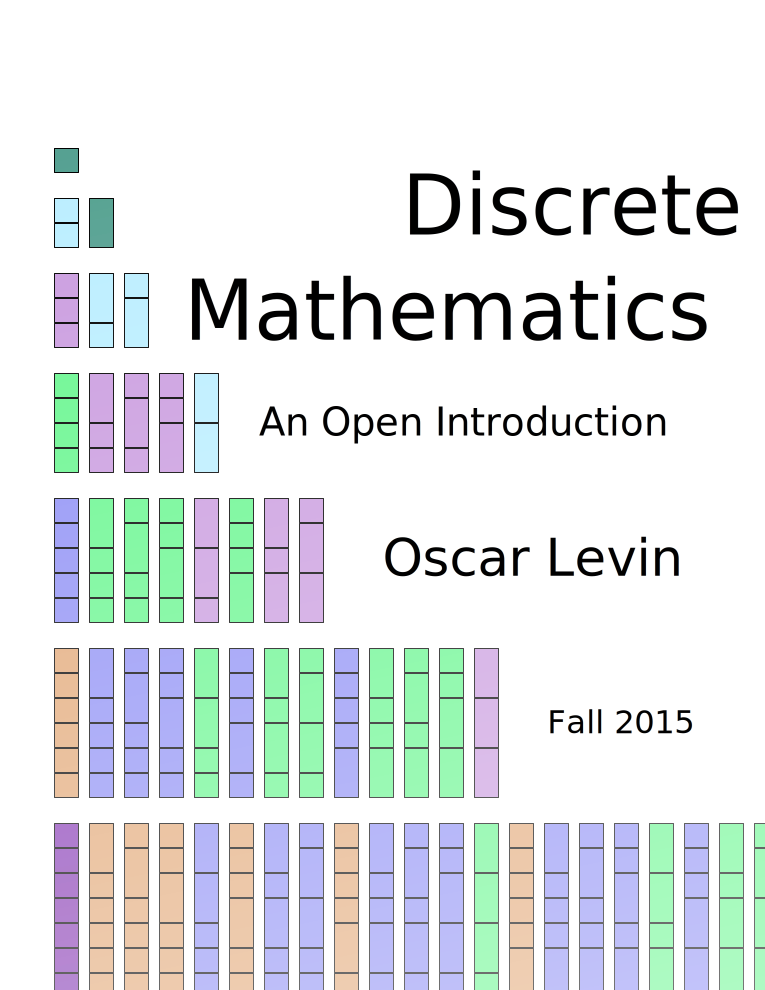
\includepdf[pages=-,pagecommand={\thispagestyle{empty}}]{frontmatter/cover2}
%
%

\clearpage






%\addtocontents{toc}{\protect\thispagestyle{plain}}

%% end: title page
%% begin: copyright-page
\thispagestyle{empty}
\vskip 3em

\noindent Oscar Levin \\ School of Mathematical Science \\ University of Northern Colorado \\ Greely, Co 80639 \\ \nolinkurl{oscar.levin@unco.edu} \\ \url{http://math.oscarlevin.com/}

\vfill
\vfill

\noindent\textcopyright ~ 2013-2016 by Oscar Levin

\vskip 3em

\noindent\includegraphics[scale=.5]{frontmatter/by-sa}\\
This work is licensed under the Creative Commons Attribution-ShareAlike 4.0 International License. To view a copy of this license, visit \url{http://creativecommons.org/licenses/by-sa/4.0/}.

\vskip 3em

\noindent Fall 2015 Edition
\vskip 1em
\noindent ISBN-10: 1516921186\\
\noindent ISBN-13: 978-1516921188
\vfill

\noindent A current version can always be found for free at \url{http://discretetext.oscarlevin.com/}
\vskip 2em

\noindent Cover image: \emph{Tiling with Fibonacci and Pascal}.
\clearpage

\vskip 2em
%% end:   copyright-page
%% begin: dedication-page
\cleardoublepage
\thispagestyle{empty}
\vspace*{\stretch{1}}
\begin{flushright}\large%
For Madeline and Teagan%
\end{flushright}
\vspace*{\stretch{2}}
\clearpage
%% end:   dedication-page
%% begin: obverse-dedication-page (empty)
\thispagestyle{empty}
\null%
\clearpage
%% end:   obverse-dedication-page
%% begin: acknowledgement
\chapter*{Acknowledgements}\label{acknowledgement-1}
\addcontentsline{toc}{chapter}{Acknowledgements}
\hypertarget{p-2}{}%
This book would not exist if not for ``Discrete and Combinatorial Mathematics'' by Richard Grassl and Tabitha Mingus. It is the book I learned discrete math out of, and taught out of the semester before I began writing this text. I wanted to maintain the inquiry based feel of their book but update, expand and rearrange some of the material.  Some of the best exposition and exercises here were graciously donated from this source.%
\par
\hypertarget{p-3}{}%
Thanks to Alees Seehausen who co-taught the Discrete Mathematics course with me in 2015 and helped develop many of the \emph{Investigate!} activities and other problems currently used in the text. She also offered many suggestions for improvement of the expository text, for which I am quite grateful. Thanks also to Katie Morrison and Nate Eldredge for their suggestions after using parts of this text in their class.%
\par
\hypertarget{p-4}{}%
While odds are that there are still errors and typos in the current book, there are many fewer thanks to the work of Michelle Morgan over the summer of 2016.%
\par
\hypertarget{p-5}{}%
The book is now available in an interactive online format, and this is entirely thanks to the work of Rob Beezer and David Farmer along with the rest of the participants of the \href{https://groups.google.com/forum/?fromgroups\#!forum/mathbook-xml-support}{mathbook-xml-support group}.  Thanks for%
\par
\hypertarget{p-6}{}%
Finally, a thank you to the numerous students who have pointed out typos and made suggestions over the years and a thanks in advance to those who will do so in the future.%
%% end:   acknowledgement
%% begin: preface
\chapter*{Preface}\label{preface}
\addcontentsline{toc}{chapter}{Preface}
\hypertarget{p-7}{}%
This text aims to give an introduction to select topics in discrete mathematics at a level appropriate for first or second year undergraduate math majors, especially those who intend to teach middle and high school mathematics. The book began as a set of notes for the Discrete Mathematics course at the University of Northern Colorado. This course serves both as a survey of the topics in discrete math and as the ``bridge'' course for math majors, as UNC does not offer a separate ``introduction to proofs'' course. Most students who take the course plan to teach, although there are a handful of students who will go on to graduate school or study applied math or computer science. For these students the current text hopefully is still of interest, but the intent is not to provide a solid mathematical foundation for computer science, unlike the majority of textbooks on the subject.%
\par
\hypertarget{p-8}{}%
Another difference between this text and most other discrete math books is that this book is intended to be used in a class taught using problem oriented or inquiry based methods. When I teach the class, I will assign sections for reading \emph{after} first introducing them in class by using a mix of group work and class discussion on a few interesting problems. The text is meant to consolidate what we \emph{discover} in class and serve as a reference for students as they master the concepts and techniques covered in the unit. None-the-less, every attempt has been made to make the text sufficient for self study as well, in a way that hopefully mimics an inquiry based classroom.%
\par
\hypertarget{p-9}{}%
The topics covered in this text were chosen to match the needs of the students I teach at UNC. The main areas of study are combinatorics, sequences, logic and proofs, and graph theory, in that order. Induction is covered at the end of the chapter on sequences. Most discrete books put logic first as a preliminary, which certainly has its advantages. However, I wanted to discuss logic and proofs together, and found that doing both of these before anything else was overwhelming for my students given that they didn't yet have context of other problems in the subject. Also, after spending a couple weeks on proofs, we would hardly use that at all when covering combinatorics, so much of the progress we made was quickly lost.  Instead, there is a short introduction section on mathematical statements, which should provide enough common language to discuss the logical content of combinatorics and sequences.%
\par
\hypertarget{p-10}{}%
Depending on the speed of the class, it might be possible to include additional material. In past semesters I have included generating functions (after sequences) and some basic number theory (either after the logic and proofs chapter or at the very end of the course). These additional topics are covered in the last chapter.%
\par
\hypertarget{p-11}{}%
While I (currently) believe this selection and order of topics is optimal, you should feel free to skip around to what interests you. There are occasionally examples and exercises that rely on earlier material, but I have tried to keep these to a minimum and usually can either be skipped or understood without too much additional study. If you are an instructor, feel free to edit the \LaTeX{} or Mathbook XML source to fit your needs.%
\typeout{************************************************}
\typeout{Paragraphs  Previous and future editions}
\typeout{************************************************}
\paragraph[{Previous and future editions}]{Previous and future editions}\hypertarget{pref_editions}{}
\hypertarget{p-12}{}%
This current 2nd edition brings a few major improvements, as well as \emph{lots} of minor corrections.  The highlights include: \leavevmode%
\begin{itemize}[label=\textbullet]
\item{}Some of the material from chapter 3 (on logic) is now part of an introduction section on mathematical statements.%
\item{}Content from the section on counting functions (previously 1.7) is now integrated with the rest of chapter 1.%
\item{}To accommodate instructors, some of the solutions to exercises were removed, and the more involved ``homework'' problems were integrated in the main exercises. New exercises and examples were added.  Currently there are about 360 exercises of which roughly 2/3 have solutions or answers.%
\item{}Behind the scenes, the source of the text transitioned from \LaTeX{} to Mathbook XML, which allows for conversion to \LaTeX{} as well as the creation of an interactive online version.%
\end{itemize}
%
\par
\hypertarget{p-13}{}%
The previous \emph{Fall 2015 edition} was essentially the first edition of the book. I had previously compiled many of the sections in a book format for easy distribution, but those were mostly just lecture notes and exercises (there was no index or Investigate problems; very little in the way of consistent formatting).%
\par
\hypertarget{p-14}{}%
My intent is to compile a new edition prior to each fall semester which incorporate additions and corrections suggested by instructors and students who use the text the previous semesters. Thus I encourage you to send along any suggestions and comments as you have them.%
\par\hfill\begin{tabular}{l@{}}
Oscar Levin, Ph.D.\\
University of Northern Colorado, 2016
\end{tabular}\\\par
%% end:   preface
%% begin: preface
\chapter*{How to use this book}\label{preface-2}
\addcontentsline{toc}{chapter}{How to use this book}
\hypertarget{p-15}{}%
In addition to expository text, this book has a few features designed to encourage you to interact with the mathematics.%
\typeout{************************************************}
\typeout{Paragraphs  \emph{Investigate!} activities}
\typeout{************************************************}
\paragraph[{\emph{Investigate!} activities}]{\emph{Investigate!} activities}\hypertarget{paragraphs-2}{}
\hypertarget{p-16}{}%
Sprinkled throughout the sections (usually at the very beginning of a topic) you will find activities designed to get you acquainted with the topic soon to be discussed. These are similar (sometimes identical) to group activities I give students to introduce material. You really should spend some time thinking about, or even working through, these problems before reading the section. By priming yourself to the types of issues involved in the material you are about to read, you will better understand what is to come. There are no solutions provided for these problems, but don't worry if you can't solve them or are not confident in your answers. My hope is that you will take this frustration with you while you read the proceeding section. By the time you are done with the section, things should be much clearer.%
\typeout{************************************************}
\typeout{Paragraphs  Examples}
\typeout{************************************************}
\paragraph[{Examples}]{Examples}\hypertarget{paragraphs-3}{}
\hypertarget{p-17}{}%
I have tried to include the ``correct'' number of examples. For those examples which include \emph{problems}, full solutions are included. Before reading the solution, try to at least have an understanding of what the problem is asking. Unlike some textbooks, the examples are not meant to be all inclusive for problems you will see in the exercises. They should not be used as a blueprint for solving other problems. Instead, use the examples to deepen our understanding of the concepts and techniques discussed in each section. Then use this understanding to solve the exercises at the end of each section.%
\typeout{************************************************}
\typeout{Paragraphs  Exercises}
\typeout{************************************************}
\paragraph[{Exercises}]{Exercises}\hypertarget{paragraphs-4}{}
\hypertarget{p-18}{}%
You get good at math through practice. Each section concludes with a small number of exercises meant to solidify concepts and basic skills presented in that section. At the end of each chapter, a larger collection of similar exercises is included (as a sort of ``chapter review'') which might bridge material of different sections in that chapter. Many exercise have a hint, answer or full solution (which in the pdf version of the text can be found by clicking on the exercises number\textemdash{}clicking on the solution number will bring you back to the exercise). Readers are encouraged to try these exercises before looking at the solution. When I teach with this book, I assign these exercises as practice and then use them, or similar problems, on quizzes and exams.  There are also problems without answers to challenge yourself (or to be assigned as homework).%
%% end:   preface
%% begin: table of contents
%% Adjust Table of Contents
\setcounter{tocdepth}{2}
\renewcommand*\contentsname{Contents}
\tableofcontents
%% end:   table of contents
\mainmatter
\typeout{************************************************}
\typeout{Chapter 0 Sequences}
\typeout{************************************************}
\chapter[{Sequences}]{Sequences}\label{ch_sequences}
\begin{investigation}[]\label{investigation-1}
\hypertarget{p-19}{}%
There is a monastery in Hanoi\index{Hanoi}, as the legend goes, with a great hall containing three tall pillars. Resting on the first pillar are 64 giant disks (or washers), all different sizes, stacked from largest to smallest. The monks are charged with the following task: they must move the entire stack of disks to the third pillar. However, due to the size of the disks, the monks cannot move more than one at a time. Each disk must be placed on one of the pillars before the next disk is moved. And because the disks are so heavy and fragile, the monks may never place a larger disk on top of a smaller disk. When the monks finally complete their task, the world shall come to an end. Your task: figure out how long before we need to start worrying about the end of the world. %
\begin{enumerate}
\item\hypertarget{li-5}{}\hypertarget{p-20}{}%
First, let's find the minimum number of moves required for a smaller number of disks. Collect some data. Make a table.%
\item\hypertarget{li-6}{}\hypertarget{p-21}{}%
Conjecture a formula for the minimum number of moves required to move \(n\) disks. Test your conjecture. How do you know your formula is correct?%
\item\hypertarget{li-7}{}\hypertarget{p-22}{}%
If the monks were able to move one disk every second without ever stopping, how long before the world ends?%
\end{enumerate}
%
\end{investigation}
\hypertarget{p-23}{}%
This puzzle is called the \emph{Tower of Hanoi}\index{Tower of Hanoi}. You are tasked with finding the minimum number of moves to complete the puzzle. This certainly sounds like a counting problem. Perhaps you have an answer? If not, what else could we try?%
\par
\hypertarget{p-24}{}%
The answer depends on the number of disks you need to move. In fact, we could answer the puzzle first for 1 disk, then 2, then 3 and so on. If we list out all of the answers for each number of disks, we will get a \terminology{sequence} of numbers. The \(n\)th term in the sequence is the answer to the question, ``what is the smallest number of moves required to complete the Tower of Hanoi puzzle with \(n\) disks?'' You might wonder why we would create such a sequence instead of just answering the question. By looking at how the sequence of numbers grows, we gain insight into the problem. It is easy to count the number of moves required for a small number of disks. We can then look for a pattern among the first few terms of the sequence. Hopefully this will suggest a method for finding the \(n\)th term of the sequence, which is the answer to our question. Of course we will also need to verify that our suspected pattern is correct, and that this correct pattern really does give us the \(n\)th term we think it does, but it is impossible to prove that your formula is correct without having a formula to start with.%
\par
\hypertarget{p-25}{}%
Sequences are also interesting mathematical objects to study in their own right. Let's see why.%
\typeout{************************************************}
\typeout{Section 0.1 Definitions}
\typeout{************************************************}
\section[{Definitions}]{Definitions}\label{sec_seq_intro}
\begin{investigation}[]\label{investigation-2}
\hypertarget{p-26}{}%
What comes next:%
\begin{equation*}
1, ~~11, ~~21, ~~1211, ~~111221, ~~312211, ~~\ldots
\end{equation*}
%
\end{investigation}
\hypertarget{p-27}{}%
A \terminology{sequence}\index{sequence} is simply an ordered list of numbers. For example, here is a sequence: 0, 1, 2, 3, 4, 5, \textellipsis{}. This is different from the set \(\N\) because, while the sequence is a complete list of every element in the set of natural numbers, in the sequence we very much care what order the numbers come in. For this reason, when we use variables to represent terms in a sequence they will look like this:%
\begin{equation*}
a_0, a_1, a_2, a_3, \ldots
\end{equation*}
To refer to the \emph{entire} sequence at once, we will write \((a_n)_{n\in\N}\) or \((a_n)_{n\ge 0}\), or sometimes if we are being sloppy, just \((a_n)\) (in which case we assume we start the sequence with \(a_0\)). \label{notation-1}
%
\par
\hypertarget{p-28}{}%
We might replace the \(a\) with another letter, and sometimes we omit \(a_0\), starting with \(a_1\), in which case we would use \((a_n)_{n \ge 1}\) to refer to the sequence as a whole. The numbers in the subscripts are called \terminology{indices} (the plural of \terminology{index}).%
\par
\hypertarget{p-29}{}%
While we often just think of sequences as an ordered list of numbers, they really are a type of function. Specifically, the sequence \((a_n)_{n\ge 0}\) is a function with domain \(\N\) where \(a_n\) is the image of the natural number \(n\). Later we will manipulate sequences in much the same way you have manipulated functions in algebra or calculus. We can shift a sequence up or down, add two sequences, or ask for the rate of change of a sequence. These are done exactly as you would for functions.%
\par
\hypertarget{p-30}{}%
That said, while keeping the rigorous mathematical definition in mind is helpful, we often describe sequences by writing out the first few terms.%
\begin{example}[]\label{example-1}
\hypertarget{p-31}{}%
Can you find the next term in the following sequences?%
\par
\hypertarget{p-32}{}%
\leavevmode%
\begin{enumerate}
\item\hypertarget{li-8}{}\(7,7,7,7,7, \ldots\)%
\item\hypertarget{li-9}{}\(3, -3, 3, -3, 3, \ldots\)%
\item\hypertarget{li-10}{}\(1, 5, 2, 10, 3, 15, \ldots\)%
\item\hypertarget{li-11}{}\(1, 2, 4, 8, 16, 32, \ldots\)%
\item\hypertarget{li-12}{}\(1, 4, 9, 16, 25, 36, \ldots\)%
\item\hypertarget{li-13}{}\(1, 2, 3, 5, 8, 13, 21, \ldots\)%
\item\hypertarget{li-14}{}\(1, 3, 6, 10, 15, 21, \ldots\)%
\item\hypertarget{li-15}{}\(2, 3, 5, 7, 11, 13, \ldots\)%
\item\hypertarget{li-16}{}\(3, 2, 1, 0, -1, \ldots\)%
\item\hypertarget{li-17}{}\(1, 1, 2, 6, \ldots\)%
\end{enumerate}
%
\par\smallskip%
\noindent\textbf{Solution.}\hypertarget{solution-1}{}\quad%
\hypertarget{p-33}{}%
No you cannot. You might guess that the next terms are:%
\par
\hypertarget{p-34}{}%
\leavevmode%
\begin{enumerate}
\item\hypertarget{li-18}{}\(7\)%
\item\hypertarget{li-19}{}\(-3\)%
\item\hypertarget{li-20}{}\(4\)%
\item\hypertarget{li-21}{}\hypertarget{p-35}{}%
64%
\item\hypertarget{li-22}{}\hypertarget{p-36}{}%
49%
\item\hypertarget{li-23}{}\hypertarget{p-37}{}%
34%
\item\hypertarget{li-24}{}\hypertarget{p-38}{}%
28%
\item\hypertarget{li-25}{}\hypertarget{p-39}{}%
17%
\item\hypertarget{li-26}{}\(-2\)%
\item\hypertarget{li-27}{}\(24\)%
\end{enumerate}
%
\par
\hypertarget{p-40}{}%
In fact, those are the next terms of the sequences I had in mind when I made up the example, but there is no way to be sure they are correct.%
\par
\hypertarget{p-41}{}%
Still, we will often do this. Given the first few terms of a sequence, we can ask what the pattern in the sequence suggests the next terms are.%
\end{example}
\hypertarget{p-42}{}%
Given that no number of initial terms in a sequence is enough to say for certain which sequence we are dealing with, we need to find another way to specify a sequence. We consider two ways to do this:%
\begin{assemblage}[Closed formula]\label{assemblage-1}
\hypertarget{p-43}{}%
A \terminology{closed formula}\index{closed formula} for a sequence \((a_n)_{n\in\N}\) is a formula for \(a_n\) using a fixed finite number of operations on \(n\). This is what you normally think of as a formula in \(n\), just like if you were defining a function in terms of \(n\) (because that is exactly what you are doing).%
\end{assemblage}
\begin{assemblage}[Recursive definition]\label{assemblage-2}
\hypertarget{p-44}{}%
A \terminology{recursive definition}\index{recursive definition} (sometimes called an \terminology{inductive definition}) for a sequence \((a_n)_{n\in\N}\) consists of a \terminology{recurrence relation}\index{recurrence relation}: an equation relating a term of the sequence to previous terms (terms with smaller index) and an \terminology{initial condition}: a list of a few terms of the sequence (one less than the number of terms in the recurrence relation).%
\end{assemblage}
\hypertarget{p-45}{}%
It is easier to understand what is going on here with an example:%
\begin{example}[]\label{example-2}
\hypertarget{p-46}{}%
Here are a few closed formulas for sequences: \leavevmode%
\begin{itemize}[label=\textbullet]
\item{}\(a_n = n^2\).%
\item{}\(\d a_n = \frac{n(n+1)}{2}\).%
\item{}\(\d a_n = \frac{\left(\frac{1 + \sqrt 5}{2}\right)^n - \left(\frac{1 + \sqrt 5}{2}\right)^{-n}}{5}\).%
\end{itemize}
%
\par
\hypertarget{p-47}{}%
Note in each case, if you are given \(n\), you can calculate \(a_n\) directly: just plug in \(n\).  For example, to find \(a_3\) in the second sequence, just compute \(a_3 = \frac{3(3+1)}{2} = 6\).%
\par
\hypertarget{p-48}{}%
Here are a few recursive definitions for sequences: \leavevmode%
\begin{itemize}[label=\textbullet]
\item{}\(a_n = 2a_{n-1}\) with \(a_0 = 1\).%
\item{}\(a_n = 2a_{n-1}\) with \(a_0 = 27\).%
\item{}\(a_n = a_{n-1} + a_{n-2}\) with \(a_0 = 0\) and \(a_1 = 1\).%
\end{itemize}
%
\par
\hypertarget{p-49}{}%
In these cases, if you are given \(n\), you cannot calculate \(a_n\) directly, you first need to find \(a_{n-1}\) (or \(a_{n-1}\) and \(a_{n-2}\)). In the second sequence, to find \(a_3\) you would take \(2a_2\), but to find \(a_2 = 2a_1\) we would need to know \(a_1 = 2a_0\).  We do know this, so we could trace back through these equations to find \(a_1 = 54\), \(a_2 = 108\) and finally \(a_3 = 216\).\index{Fibonacci sequence}%
\end{example}
\begin{investigation}[]\label{investigation-3}
\hypertarget{p-50}{}%
You have a large collection of \(1\times 1\) squares and \(1\times 2\) dominoes. You want to arrange these to make a \(1 \times 15\) strip. How many ways can you do this? %
\begin{enumerate}
\item\hypertarget{li-34}{}\hypertarget{p-51}{}%
Start by collecting data. How many length \(1\times 1\) strips can you make? How many \(1\times 2\) strips? How many \(1\times 3\) strips? And so on.%
\item\hypertarget{li-35}{}\hypertarget{p-52}{}%
How are the \(1\times 3\) and \(1 \times 4\) strips related to the \(1\times 5\) strips?%
\item\hypertarget{li-36}{}\hypertarget{p-53}{}%
How many \(1\times 15\) strips can you make?%
\item\hypertarget{li-37}{}\hypertarget{p-54}{}%
What if I asked you to find the number of \(1\times 1000\) strips? Would the method you used to calculate the number fo \(1 \times 15\) strips be helpful?%
\end{enumerate}
%
\end{investigation}
\hypertarget{p-55}{}%
You might wonder why we would bother with recursive definitions for sequences. After all, it is harder to find \(a_n\) with a recursive definition than with a closed formula. This is true, but it is also harder to find a closed formula for a sequence than it is to find a recursive definition. So to find a useful closed formula, we might first find the recursive definition, then use that to find the closed formula.%
\par
\hypertarget{p-56}{}%
This is not to say that recursive definitions aren't useful in finding \(a_n\). You can always calculate \(a_n\) given a recursive definition, it might just take a while.%
\begin{example}[]\label{example-3}
\hypertarget{p-57}{}%
Find \(a_6\) in the sequence defined by \(a_n = 2a_{n-1} - a_{n-2}\) with \(a_0 = 3\) and \(a_1 = 4\).%
\par\smallskip%
\noindent\textbf{Solution.}\hypertarget{solution-2}{}\quad%
\hypertarget{p-58}{}%
We know that \(a_6 = 2a_5 - a_4\). So to find \(a_6\) we need to find \(a_5\) and \(a_4\). Well%
\begin{equation*}
a_5 = 2a_4 - a_3 \qquad \text{and} \qquad a_4 = 2a_3 - a_2,
\end{equation*}
so if we can only find \(a_3\) and \(a_2\) we would be set. Of course%
\begin{equation*}
a_3 = 2a_2 - a_1 \qquad \text{and} \qquad a_2 = 2a_1 - a_0,
\end{equation*}
so we only need to find \(a_1\) and \(a_0\). But we are given these. Thus%
\begin{align*}
a_0 \amp = 3\\
a_1 \amp = 4\\
a_2 \amp = 2\cdot 4 - 3 = 5\\
a_3 \amp = 2\cdot 5 - 4 = 6\\
a_4 \amp = 2\cdot 6 - 5 = 7\\
a_5 \amp = 2\cdot 7 - 6 = 8\\
a_6 \amp = 2\cdot 8 - 7 = 9.
\end{align*}
%
\par
\hypertarget{p-59}{}%
Note that now we can guess a closed formula for the \(n\)th term of the sequence: \(a_n = n+3\). To be sure this will always work, we could plug in this formula into the recurrence relation:%
\begin{align*}
2a_{n-1} - a_{n-2} \amp = 2((n-1) + 3) - ((n-2) + 3)\\
\amp = 2n + 4 - n - 1 \\
\amp = n + 3\\
\amp = a_n.
\end{align*}
%
\par
\hypertarget{p-60}{}%
That is not quite enough though, since there can be multiple closed formulas that satisfy the same recurrence relation; we must also check that our closed formula agrees on the initial terms of the sequence.  Since \(a_0 = 0 + 3 = 3\) and \(a_1 = 1+3 = 4\) are the correct initial conditions, we can now conclude we have the correct closed formula.%
\end{example}
\hypertarget{p-61}{}%
Finding closed formulas, or even recursive definitions, for sequences is not trivial. There is no one method for doing this. Just like in evaluating integrals or solving differential equations, it is useful to have a bag of tricks you can apply, but sometimes there is no easy answer.%
\par
\hypertarget{p-62}{}%
One useful method is to relate a given sequence to another sequence for which we already know the closed formula.%
\begin{example}[]\label{example-4}
\hypertarget{p-63}{}%
Use the formulas \(T_n = \frac{n(n+1)}{2}\) and \(a_n = 2^n\) to find closed formulas for the following sequences. \leavevmode%
\begin{enumerate}
\item\hypertarget{li-38}{}\hypertarget{p-64}{}%
\((b_n)\): \(1, 2, 4, 7, 11, 16, 22, \ldots \).%
\item\hypertarget{li-39}{}\hypertarget{p-65}{}%
\((c_n)\): \(3, 5, 9, 17, 33,\ldots \).%
\item\hypertarget{li-40}{}\hypertarget{p-66}{}%
\((d_n)\): \(0, 2, 6, 12, 20, 30, 42,\ldots \).%
\item\hypertarget{li-41}{}\hypertarget{p-67}{}%
\((e_n)\): \(3, 6, 10, 15, 21, 28, \ldots\).%
\item\hypertarget{li-42}{}\hypertarget{p-68}{}%
\((f_n)\): \(0, 1, 3, 7, 15, 31, \ldots \).%
\item\hypertarget{li-43}{}\hypertarget{p-69}{}%
\((g_n)\) \(3, 6, 12, 24, 48, \ldots \).%
\item\hypertarget{li-44}{}\hypertarget{p-70}{}%
\((h_n)\): \(6, 10, 18, 34, 66, \ldots \).%
\item\hypertarget{li-45}{}\hypertarget{p-71}{}%
\((j_n)\): \(15, 33, 57, 87, 123, \ldots\).%
\end{enumerate}
%
\par\smallskip%
\noindent\textbf{Solution.}\hypertarget{solution-3}{}\quad%
\hypertarget{p-72}{}%
Before you say this is impossible, what we are asking for is simply to find a closed formula which agrees with all of the initial terms of the sequences. Of course there is no way to read into the mind of the person who wrote the numbers down, but we can at least do this.%
\par
\hypertarget{p-73}{}%
The first few terms of \((T_n)_{n\ge 0}\)\label{notation-2}
 are \(0, 1, 3, 6, 10, 15, 21, \ldots\) (these are called the \terminology{triangular numbers})\index{triangular numbers}. The first few terms of \((a_n)_{n\ge 0}\) are \(1, 2, 4, 8, 16, \ldots\).  Let's try to find formulas for the given sequences: \leavevmode%
\begin{enumerate}
\item\hypertarget{li-46}{}\hypertarget{p-74}{}%
\((1, 2, 4, 7, 11, 16, 22, \ldots)\). Note that if subtract 1 from each term, we get the sequence \((T_n)\). So we have \(b_n = T_n + 1\). Therefore a closed formula is \(b_n = \frac{n(n+1)}{2} + 1\). A quick check of the first few \(n\) confirms we have it right.%
\item\hypertarget{li-47}{}\hypertarget{p-75}{}%
\((3, 5, 9, 17, 33, \ldots )\). Each term in this sequence is one more than a power of 2, so we might guess the closed formula is \(c_n = a_n+1 = 2^n + 1\). If we try this though, we get \(c_0 2^0 + 1 = 2\) and \(c_1 = 2^1 + 1 = 3\). We are off because the indices are shifted.  What we really want is \(c_n = a_{n+1}+1\) giving  \(c_n = 2^{n+1} + 1\).%
\item\hypertarget{li-48}{}\hypertarget{p-76}{}%
(\(0, 2, 6, 12, 20, 30, 42,\ldots \)). Notice that all these terms are even. What happens if we factor out a 2? We get \((T_n)\)! More precisely, we find that \(d_n/2 = T_n\), so this sequence has closed formula \(d_n = n(n+1)\).%
\item\hypertarget{li-49}{}\hypertarget{p-77}{}%
\((3, 6, 10, 15, 21, 28, \ldots)\). These are all triangular numbers. However, we are starting with 3 as our initial term instead of as our third term. So if we could plug in 2 instead of 0 into the formula for \(T_n\), we would be set. Therefore the closed formula is \(e_n = \frac{(n+2)(n+3)}{2}\) (where \(n+3\) came from \((n+2)+1\)).  Thinking about sequences as functions, we are doing a horizontal shift by 2: \(e_n = T_{n+2}\) which would cause the graph to shift 2 units to the left.%
\item\hypertarget{li-50}{}\hypertarget{p-78}{}%
\((0, 1, 3, 7, 15, 31, \ldots )\). Try adding 1 to each term and we get powers of 2. You might guess this because each term is a little more than twice the previous term (the powers of 2 are \emph{exactly} twice the previous term). Closed formula: \(f_n = 2^{n} - 1\).%
\item\hypertarget{li-51}{}\hypertarget{p-79}{}%
\((3, 6, 12, 24, 48, \ldots )\). These numbers are also doubling each time, but are also all multiples of 3. Dividing each by 3   gives 1, 2, 4, 8, \textellipsis{}. Aha. We get the closed formula \(g_n = 3\cdot 2^{n}\).%
\item\hypertarget{li-52}{}\hypertarget{p-80}{}%
\((6, 10, 18, 34, 66, \ldots )\). To get from one term to the next, we almost double each term. So maybe we can relate this back to \(2^n\). Yes, each term is 2 more than a power of 2. So we get \(h_n = 2^{n+2} + 2\) (the \(n+2\) is because the first term is 2 more than \(2^2\), not \(2^0\)). Alternatively, we could have related this sequence to the second sequence in this example: starting with 3, 5, 9, 17, \textellipsis{} we see that this sequence is twice the terms from that sequence. That sequence had closed formula \(c_n = 2^{n+1} + 1\). Our sequence here would be twice this, so \(h_n = 2(2^n + 1)\), which is the same as we got before.%
\item\hypertarget{li-53}{}\hypertarget{p-81}{}%
\((15, 33, 57, 87, 123, \ldots)\). Try dividing each term by 3. That gives the sequence \(5, 11, 19, 29, 41,\ldots\). Now add 1: \(6, 12, 20, 30, 42, \ldots\), which is \((d_n)\) in this example, except starting with 6 instead of 0. So let's start with the formula \(d_n= n(n+1)\). To start with the 6, we shift: \((n+2)(n+3)\). But this is one too many, so subtract 1: \((n+2)(n+3) - 1\). That gives us our sequence, but divided by 3. So we want \(j_n = 3((n+2)(n+3) - 1)\).%
\end{enumerate}
%
\end{example}
\typeout{************************************************}
\typeout{Exercises  Exercises}
\typeout{************************************************}
\subsection[{Exercises}]{Exercises}\label{exercises_seq_basics}
\begin{exerciselist}
\item[1.]\hypertarget{exercise-1}{}\hypertarget{p-82}{}%
Find the closed formula for each of the following sequences by relating them to a well known sequence. Assume the first term given is \(a_1\).%
\leavevmode%
\begin{enumerate}[label=(\alph*)]
\item\hypertarget{li-54}{}\(2, 5, 10, 17, 26, \ldots\)%
\item\hypertarget{li-55}{}\(0, 2, 5, 9, 14, 20, \ldots\)%
\item\hypertarget{li-56}{}\(8, 12, 17, 23, 30,\ldots\)%
\item\hypertarget{li-57}{}\(1, 5, 23, 119, 719,\ldots\)%
\end{enumerate}
\par\smallskip
\item[2.]\hypertarget{exercise-2}{}\hypertarget{p-84}{}%
For each sequence given below, find a closed formula for \(a_n\), the \(n\)th term of the sequence (assume the first terms are \(a_0\)) by relating it to another sequence for which you already know the formula. In each case, briefly say how you got your answers.%
\leavevmode%
\begin{enumerate}[label=(\alph*)]
\item\hypertarget{li-62}{}\hypertarget{p-85}{}%
4, 5, 7, 11, 19, 35, \textellipsis{} %
\item\hypertarget{li-63}{}\hypertarget{p-86}{}%
0, 3, 8, 15, 24, 35, \textellipsis{} %
\item\hypertarget{li-64}{}\hypertarget{p-87}{}%
6, 12, 20, 30, 42, \textellipsis{} %
\item\hypertarget{li-65}{}\hypertarget{p-88}{}%
0, 2, 7, 15, 26, 40, 57, \textellipsis{} (Cryptic Hint: these might be called ``house numbers'') %
\end{enumerate}
\par\smallskip
\item[3.]\hypertarget{exercise-3}{}\hypertarget{p-89}{}%
The Fibonacci sequence is \(0, 1, 1, 2, 3, 5, 8, 13, \ldots\) (where \(F_0 = 0\)).\index{Fibonacci sequence}%
\par
\hypertarget{p-90}{}%
\leavevmode%
\begin{enumerate}[label=(\alph*)]
\item\hypertarget{li-66}{}\hypertarget{p-91}{}%
Give the recursive definition for the sequence.%
\item\hypertarget{li-67}{}\hypertarget{p-92}{}%
Write out the first few terms of the sequence of partial sums: \(0\), \(0+1\), \(0+1+1\),\textellipsis{}%
\item\hypertarget{li-68}{}\hypertarget{p-93}{}%
Give a closed formula for the sequence of partial sums in terms of \(F_n\)\label{notation-3}
 (for example, you might say \(F_0 + F_1 + \cdots + F_n = 3F_{n-1}^2 + n\), although that is definitely not correct).%
\end{enumerate}
%
\par\smallskip
\item[4.]\hypertarget{exercise-4}{}\hypertarget{p-95}{}%
Consider the three sequences below. For each, find a recursive definition. How are these sequences related?%
\par
\hypertarget{p-96}{}%
\leavevmode%
\begin{enumerate}[label=(\alph*)]
\item\hypertarget{li-72}{}\(2, 4, 6, 10, 16, 26, 42, \ldots\).%
\item\hypertarget{li-73}{}\(5, 6, 11, 17, 28, 45, 73, \ldots\).%
\item\hypertarget{li-74}{}\(0, 0 , 0 , 0 , 0 , 0 , 0 ,\ldots\).%
\end{enumerate}
%
\par\smallskip
\item[5.]\hypertarget{exercise-5}{}\hypertarget{p-98}{}%
Show that \(a_n = 3\cdot 2^n + 7\cdot 5^n\) is a solution to the recurrence relation \(a_n = 7a_{n-1} - 10a_{n-2}\).   What would the initial conditions need to be for this to be the closed formula for the sequence?%
\par\smallskip
\item[6.]\hypertarget{exercise-6}{}\hypertarget{p-99}{}%
Write out the first few terms of the sequence given by \(a_1 = 3\); \(a_n = 2a_{n-1} + 4\). Then find a recursive definition for the sequence \(10, 24, 52, 108, \ldots\).%
\par\smallskip
\item[7.]\hypertarget{exercise-7}{}\hypertarget{p-100}{}%
Write out the first few terms of the sequence given by \(a_n = n^2 - 3n + 1\). Then find a closed formula for the sequence (starting with \(a_1\)) \(0, 2, 6, 12, 20, \ldots\).%
\par\smallskip
\item[8.]\hypertarget{exercise-8}{}\hypertarget{p-101}{}%
Find a closed formula for the sequence with recursive definition \(a_n = 2a_{n-1} - a_{n-2}\) with \(a_1 = 1\) and \(a_2 = 2\).%
\par\smallskip
\item[9.]\hypertarget{exercise-9}{}\hypertarget{p-102}{}%
Find a recursive definition for the sequence with closed formula \(a_n = 3 + 2n\). Bonus points if you can give a recursive definition in which makes use of two previous terms and no constants.%
\par\smallskip
\end{exerciselist}
\typeout{************************************************}
\typeout{Section 0.2 Arithmetic and Geometric Sequences}
\typeout{************************************************}
\section[{Arithmetic and Geometric Sequences}]{Arithmetic and Geometric Sequences}\label{sec_seq-arithgeom}
\begin{investigation}[]\label{investigation-4}
\hypertarget{p-103}{}%
For the patterns of dots below, draw the next pattern in the sequence. Then give a recursive definition and a closed formula for the number of dots in the \(n\)th pattern.%
\par
\hypertarget{p-104}{}%
%
\begin{enumerate}
\item\hypertarget{li-75}{}% group protects changes to lengths, releases boxes (?)
{% begin: group for a single side-by-side
% set panel max height to practical minimum, created in preamble
\setlength{\panelmax}{0pt}
\ifdefined\panelboxAimage\else\newsavebox{\panelboxAimage}\fi%
\begin{lrbox}{\panelboxAimage}
\resizebox{0.65\linewidth}{!}{{
        \begin{tikzpicture}
\draw[fill = black] (0,0) \v;
\node[below] at (0,-.6) {$n = 0$};

  \draw[fill = black] (0+3,0) \v (.3+3, .3) \v (-.3+3,-.3) \v (-.3+3, .3) \v (.3+3,-.3) \v;
    \node[below] at (0+3,-.6) {$n = 1$};

  \draw[fill = black] (0+6,0) \v (.3+6, .3) \v (-.3+6,-.3) \v (-.3+6, .3) \v (.3+6,-.3) \v (.6+6, .6) \v (-.6+6,-.6) \v (-.6+6, .6) \v (.6+6,-.6) \v;
    \node[below] at (0+6,-.6) {$n = 2$:};
  \end{tikzpicture}
}
}\end{lrbox}
\ifdefined\phAimage\else\newlength{\phAimage}\fi%
\setlength{\phAimage}{\ht\panelboxAimage+\dp\panelboxAimage}
\settototalheight{\phAimage}{\usebox{\panelboxAimage}}
\setlength{\panelmax}{\maxof{\panelmax}{\phAimage}}
\leavevmode%
% begin: side-by-side as tabular
% \tabcolsep change local to group
\setlength{\tabcolsep}{0\linewidth}
% @{} suppress \tabcolsep at extremes, so margins behave as intended
\par\medskip\noindent
\hspace*{0.175\linewidth}%
\begin{tabular}{@{}*{1}{c}@{}}
\begin{minipage}[c][\panelmax][t]{0.65\linewidth}\usebox{\panelboxAimage}\end{minipage}\end{tabular}\\
% end: side-by-side as tabular
}% end: group for a single side-by-side
%
\item\hypertarget{li-76}{}% group protects changes to lengths, releases boxes (?)
{% begin: group for a single side-by-side
% set panel max height to practical minimum, created in preamble
\setlength{\panelmax}{0pt}
\ifdefined\panelboxAimage\else\newsavebox{\panelboxAimage}\fi%
\begin{lrbox}{\panelboxAimage}
\resizebox{0.65\linewidth}{!}{{
        \begin{tikzpicture}
\draw[fill = black] (0,0) \v (0,2) \v;
\node[below] at (0,0) {$n = 0$};

  \draw[fill = black] (-.5+3,0) \v (.5+3, 0) \v (0+3, .7) \v (-.5+3,2) \v (.5+3, 2) \v (0+3,2.7) \v;
  \node[below] at (0+3,0) {$n = 1$};

  \draw[fill = black] (-.7+6,0) \v (-.3+6,0) \v (-.5+6,.35) \v
  	(.3+6, 0) \v (.7+6,0) \v (.5+6, .35) \v
  	(-.2+6, .7) \v (.2+6, .7) \v (0+6, 1.05) \v
  	(-.7+6, 2) \v (-.3+6, 2) \v (-.5+6,2.35) \v
  	(.3+6, 2) \v (.7+6, 2) \v (.5+6, 2.35) \v
  	(-.2+6,2.7) \v (.2+6, 2.7) \v (0+6,3.05) \v;
    \node[below] at (0+6,0) {$n = 2$};
  \end{tikzpicture}
}
}\end{lrbox}
\ifdefined\phAimage\else\newlength{\phAimage}\fi%
\setlength{\phAimage}{\ht\panelboxAimage+\dp\panelboxAimage}
\settototalheight{\phAimage}{\usebox{\panelboxAimage}}
\setlength{\panelmax}{\maxof{\panelmax}{\phAimage}}
\leavevmode%
% begin: side-by-side as tabular
% \tabcolsep change local to group
\setlength{\tabcolsep}{0\linewidth}
% @{} suppress \tabcolsep at extremes, so margins behave as intended
\par\medskip\noindent
\hspace*{0.175\linewidth}%
\begin{tabular}{@{}*{1}{c}@{}}
\begin{minipage}[c][\panelmax][t]{0.65\linewidth}\usebox{\panelboxAimage}\end{minipage}\end{tabular}\\
% end: side-by-side as tabular
}% end: group for a single side-by-side
%
\item\hypertarget{li-77}{}% group protects changes to lengths, releases boxes (?)
{% begin: group for a single side-by-side
% set panel max height to practical minimum, created in preamble
\setlength{\panelmax}{0pt}
\ifdefined\panelboxAimage\else\newsavebox{\panelboxAimage}\fi%
\begin{lrbox}{\panelboxAimage}
\resizebox{0.9\linewidth}{!}{{
        \begin{tikzpicture}
\draw[fill = black] (0,0) \v;
\node[below] at (0,-.25) {$n = 1$};

  \draw[fill = black] (0+2,0) \v (.5+2, 0) \v (.25+2,.4) \v;
  \node[below] at (.25+2,-.25) {$n = 2$};

  \draw[fill = black] (0+4,0) \v (.5+4, 0) \v (.25+4,.4) \v (1+4,0) \v (.75+4,.4) \v (.5+4, .8) \v;
  \node[below] at (.5+4,-.25) {$n = 3$};

      \draw[fill = black] (0+6,0) \v (.5+6, 0) \v (.25+6,.4) \v (1+6,0) \v (.75+6,.4) \v (.5+6, .8) \v (1.5+6, 0) \v (1.25+6, .4) \v (1+6, .8) \v (.75+6, 1.2) \v;
      \node[below] at (.75+6,-.25) {$n = 4$};
      \end{tikzpicture}
}
}\end{lrbox}
\ifdefined\phAimage\else\newlength{\phAimage}\fi%
\setlength{\phAimage}{\ht\panelboxAimage+\dp\panelboxAimage}
\settototalheight{\phAimage}{\usebox{\panelboxAimage}}
\setlength{\panelmax}{\maxof{\panelmax}{\phAimage}}
\leavevmode%
% begin: side-by-side as tabular
% \tabcolsep change local to group
\setlength{\tabcolsep}{0\linewidth}
% @{} suppress \tabcolsep at extremes, so margins behave as intended
\par\medskip\noindent
\hspace*{0.05\linewidth}%
\begin{tabular}{@{}*{1}{c}@{}}
\begin{minipage}[c][\panelmax][t]{0.9\linewidth}\usebox{\panelboxAimage}\end{minipage}\end{tabular}\\
% end: side-by-side as tabular
}% end: group for a single side-by-side
%
\end{enumerate}
%
\end{investigation}
\hypertarget{p-105}{}%
We now turn to the question of finding closed formulas for particular types of sequences.%
\begin{assemblage}[Arithmetic Sequences]\label{assemblage-3}
\hypertarget{p-106}{}%
If the terms of a sequence differ by a constant, we say the sequence is \terminology{arithmetic}\index{arithmetic sequence}. If the initial term (\(a_0\)) of the sequence is \(a\) and the \terminology{common difference} is \(d\), then we have,%
\par
\hypertarget{p-107}{}%
Recursive definition: \(a_n = a_{n-1} + d\) with \(a_0 = a\).%
\par
\hypertarget{p-108}{}%
Closed formula: \(a_n = a + dn\).%
\end{assemblage}
\hypertarget{p-109}{}%
How do we know this? For the recursive definition, we need to specify \(a_0\). Then we need to express \(a_n\) in terms of \(a_{n-1}\). If we call the first term \(a\), then \(a_0 = a\). For the recurrence relation, by the definition of an arithmetic sequence, the difference between successive terms is some constant, say \(d\). So \(a_n - a_{n-1} = d\), or in other words,%
\begin{equation*}
a_0 = a \qquad a_n=a_{n-1}+d.
\end{equation*}
%
\par
\hypertarget{p-110}{}%
To find a closed formula, first write out the sequence in general:%
\begin{align*}
a_0 \amp = a\\
a_1 \amp = a_0 + d = a+d\\
a_2 \amp = a_1 + d = a+d+d = a+2d\\
a_3 \amp = a_2 + d = a+2d+d = a+3d\\
\amp \vdots 
\end{align*}
%
\par
\hypertarget{p-111}{}%
We see that to find the \(n\)th term, we need to start with \(a\) and then add \(d\) a bunch of times. In fact, add it \(n\) times. Thus \(a_n = a+dn\).%
\begin{example}[]\label{example-5}
\hypertarget{p-112}{}%
Find recursive definitions and closed formulas for the sequences below. Assume the first term listed is \(a_0\).%
\par
\hypertarget{p-113}{}%
\leavevmode%
\begin{enumerate}
\item\hypertarget{li-78}{}\(2, 5, 8, 11, 14, \ldots\).%
\item\hypertarget{li-79}{}\(50, 43, 36, 29, \ldots\).%
\end{enumerate}
%
\par\smallskip%
\noindent\textbf{Solution.}\hypertarget{solution-7}{}\quad%
\hypertarget{p-114}{}%
First we should check that these sequences really are arithmetic by taking differences of successive terms. Doing so will reveal the common difference \(d\).%
\par
\hypertarget{p-115}{}%
\leavevmode%
\begin{enumerate}
\item\hypertarget{li-80}{}\(5-2 = 3\), \(8-5 = 3\), etc. To get from each term to the next, we add three, so \(d = 3\). The recursive definition is therefore \(a_n = a_{n-1} + 3\) with \(a_0 = 2\). The closed formula is \(a_n = 2 + 3n\).%
\item\hypertarget{li-81}{}\hypertarget{p-116}{}%
Here the common difference is \(-7\), since we add \(-7\) to 50 to get 43, and so on. Thus we have a recursive definition of \(a_n = a_{n-1} - 7\) with \(a_0 = 50\). The closed formula is \(a_n = 50 - 7n\).%
\end{enumerate}
%
\end{example}
\hypertarget{p-117}{}%
What about sequences like \(2, 6, 18, 54, \ldots\)? This is not arithmetic because the difference between terms is not constant. However, the \emph{ratio} between successive terms is constant. We call such sequences \terminology{geometric}.%
\par
\hypertarget{p-118}{}%
The recursive definition for the geometric sequence with initial term \(a\) and common ratio \(r\) is \(a_n = a_{n}\cdot r; a_0 = a\). To get the next term we multiply the previous term by \(r\). We can find the closed formula like we did for the arithmetic progression. Write%
\begin{align*}
a_0 \amp = a\\
a_1 \amp = a_0\cdot r\\
a_2 \amp = a_1 \cdot r = a_0\cdot r\cdot r = a_0\cdot r^2\\
\amp \vdots 
\end{align*}
We must multiply the first term \(a\) by \(r\) a number of times, \(n\) times to be precise. We get \(a_n = a\cdot r^{n}\).%
\begin{assemblage}[Geometric Sequences]\label{assemblage-4}
\hypertarget{p-119}{}%
A sequence is called \terminology{geometric}\index{geometric sequence} if the ratio between successive terms is constant. Suppose the initial term \(a_0\) is \(a\) and the \terminology{common ratio} is \(r\). Then we have,%
\par
\hypertarget{p-120}{}%
Recursive definition: \(a_n = ra_{n-1}\) with \(a_0 = a\).%
\par
\hypertarget{p-121}{}%
Closed formula: \(a_n = a\cdot r^{n}\).%
\end{assemblage}
\begin{example}[]\label{example-6}
\hypertarget{p-122}{}%
Find the recursive and closed formula for the sequences below. Again, the first term listed is \(a_0\). \leavevmode%
\begin{enumerate}
\item\hypertarget{li-82}{}\(3, 6, 12, 24, 48, \ldots\)%
\item\hypertarget{li-83}{}\(27, 9, 3, 1, 1/3, \ldots\)%
\end{enumerate}
%
\par\smallskip%
\noindent\textbf{Solution.}\hypertarget{solution-8}{}\quad%
\hypertarget{p-123}{}%
Again, we should first check that these sequences really are geometric, this time by dividing each term by its previous term.  Assuming this ratio is constant, we will have found \(r\). \leavevmode%
\begin{enumerate}
\item\hypertarget{li-84}{}\(6/3 = 2\), \(12/6 = 2\), \(24/12 = 2\), etc. Yes, to get from any term to the next, we multiply by \(r = 2\). So the recursive definition is \(a_n = 2a_{n-1}\) with \(a_0 = 3\). The closed formula is \(a_n = 3\cdot 2^{n}\).%
\item\hypertarget{li-85}{}\hypertarget{p-124}{}%
The common ratio is \(r = 1/3\). So the sequence has recursive definition \(a_n = \frac{1}{3}a_{n-1}\) with \(a_0 = 27\) and closed formula \(a_n = 27\cdot \frac{1}{3}^{n}\).%
\end{enumerate}
%
\end{example}
\hypertarget{p-125}{}%
In the examples and formulas above, we assumed that the \emph{initial} term was \(a_0\). If your sequence starts with \(a_1\), you can easily find the term that would have been \(a_0\) and use that in the formula. For example, if we want a formula for the sequence \(2, 5, 8,\ldots\) and insist that \(2= a_1\), then we can find \(a_0 = -1\) (since the sequence is arithmetic with common difference 3, we have \(a_0 + 3 = a_1\)). Then the closed formula will be \(a_n = -1 + 3n\).%
\begin{remark}[]\label{remark-1}
\hypertarget{p-126}{}%
If you look at other textbooks or online, you might find that their closed formulas for arithmetic and geometric sequences differ from ours.  Specifically, you might find the formulas \(a_n = a +(n-1)d\) (arithmetic) and \(a_n = a\cdot r^{n-1}\) (geometric).  Which is correct?  Both!  In our case, we take \(a\) to be \(a_0\).  If instead we had \(a_1\) as our initial term, we would get the (slightly more complicated) formulas you find elsewhere.%
\end{remark}
\typeout{************************************************}
\typeout{Subsection  Sums of Arithmetic and Geometric Sequences}
\typeout{************************************************}
\subsection[{Sums of Arithmetic and Geometric Sequences}]{Sums of Arithmetic and Geometric Sequences}\label{subsection-1}
\begin{investigation}[]\label{investigation-5}
\hypertarget{p-127}{}%
Your neighborhood grocery store has a candy machine full of Skittles. %
\begin{enumerate}
\item\hypertarget{li-86}{}\hypertarget{p-128}{}%
Suppose that the candy machine currently holds exactly 650 Skittles, and every time someone inserts a quarter, exactly 7 Skittles come out of the machine. %
\begin{enumerate}
\item\hypertarget{li-87}{}\hypertarget{p-129}{}%
How many Skittles will be left in the machine after 20 quarters have been inserted?%
\item\hypertarget{li-88}{}\hypertarget{p-130}{}%
Will there ever be exactly zero Skittles left in the machine? Explain.%
\end{enumerate}
%
\item\hypertarget{li-89}{}\hypertarget{p-131}{}%
What if the candy machine gives 7 Skittles to the first customer who put in a quarter, 10 to the second, 13 to the third, 16 to the fourth, etc. How many Skittles has the machine given out after 20 quarters are put into the machine?%
\item\hypertarget{li-90}{}\hypertarget{p-132}{}%
Now, what if the machine gives 4 Skittles to the first customer, 7 to the second, 12 to the third, 19 to the fourth, etc. How many Skittles has the machine given out after 20 quarters are put into the machine?%
\end{enumerate}
%
\end{investigation}
\hypertarget{p-133}{}%
Look at the sequence \((T_n)_{n\ge 1}\) which starts \(1, 3, 6, 10, 15,\ldots\). These are called the \terminology{triangular numbers}\index{triangular numbers} since they represent the number of dots in an equilateral triangle (think of how you arrange 10 bowling pins: a row of 4 plus a row of 3 plus a row of 2 and a row of 1).%
% group protects changes to lengths, releases boxes (?)
{% begin: group for a single side-by-side
% set panel max height to practical minimum, created in preamble
\setlength{\panelmax}{0pt}
\ifdefined\panelboxAimage\else\newsavebox{\panelboxAimage}\fi%
\begin{lrbox}{\panelboxAimage}
\resizebox{0.5\linewidth}{!}{{
  \begin{tikzpicture}
\draw[fill = black] (0,0) \v;
\node[below] at (0,-.25) {$T_1 = 1$};

\draw[fill = black] (0+2,0) \v (.5+2, 0) \v (.25+2,.4) \v;
\node[below] at (.25+2,-.25) {$T_2 = 3$};

\draw[fill = black] (0+4,0) \v (.5+4, 0) \v (.25+4,.4) \v (1+4,0) \v (.75+4,.4) \v (.5+4, .8) \v;
\node[below] at (.5+4,-.25) {$T_3 = 6$};

\draw[fill = black] (0+6,0) \v (.5+6, 0) \v (.25+6,.4) \v (1+6,0) \v (.75+6,.4) \v (.5+6, .8) \v (1.5+6, 0) \v (1.25+6, .4) \v (1+6, .8) \v (.75+6, 1.2) \v;
\node[below] at (.75+6,-.25) {$T_4 = 10$};
\end{tikzpicture}
}
}\end{lrbox}
\ifdefined\phAimage\else\newlength{\phAimage}\fi%
\setlength{\phAimage}{\ht\panelboxAimage+\dp\panelboxAimage}
\settototalheight{\phAimage}{\usebox{\panelboxAimage}}
\setlength{\panelmax}{\maxof{\panelmax}{\phAimage}}
\leavevmode%
% begin: side-by-side as tabular
% \tabcolsep change local to group
\setlength{\tabcolsep}{0\linewidth}
% @{} suppress \tabcolsep at extremes, so margins behave as intended
\par\medskip\noindent
\hspace*{0.25\linewidth}%
\begin{tabular}{@{}*{1}{c}@{}}
\begin{minipage}[c][\panelmax][t]{0.5\linewidth}\usebox{\panelboxAimage}\end{minipage}\end{tabular}\\
% end: side-by-side as tabular
}% end: group for a single side-by-side
\par
\hypertarget{p-134}{}%
Is this sequence arithmetic? No, since \(3-1 = 2\) and \(6-3 = 3 \ne 2\), so there is no common difference. Is the sequence geometric? No. \(3/1 = 3\) but \(6/3 = 2\), so there is no common ratio. What to do?%
\par
\hypertarget{p-135}{}%
Notice that the differences between terms form an arithmetic sequence: \(2, 3, 4, 5, 6,\ldots\). This says that the \(n\)th term of the sequence \(1,3,6,10,15,\ldots\) is the \emph{sum} of the first \(n\) terms in the sequence \(1,2,3,4,5,\ldots\). We say that the first sequence is the \terminology{sequence of partial sums}\index{partial sums} of the second sequence (partial sums because we are not taking the sum of all infinitely many terms). If we know how to add up the terms of an arithmetic sequence, we could use this to find a closed formula for a sequence whose differences are the terms of that arithmetic sequence.%
\par
\hypertarget{p-136}{}%
This should become clearer if we write the triangular numbers like this:%
\begin{align*}
1 \amp = 1\\
3 \amp = 1+2\\
6 \amp = 1 + 2 + 3\\
10 \amp = 1+2 + 3+ 4\\
\vdots \amp \qquad \vdots\\
T_n \amp = 1 + 2 + 3 + \cdots + n.
\end{align*}
%
\par
\hypertarget{p-137}{}%
Consider how we could find the sum of the first 100 positive integers (that is, \(T_{100}\)). Instead of adding them in order, we regroup and add \(1+100 = 101\). The next pair to combine is \(2+99 = 101\). Then \(3+98 = 101\). Keep going. This gives 50 pairs which each add up to \(101\), so \(T_{100} = 101\cdot 50 = 5050\).\footnote{This insight is usually attributed to Carl Friedrich Gauss, one of the greatest mathematicians of all time, who discovered it as a child when his unpleasant elementary teacher thought he would keep the class busy by requiring them to compute the lengthy sum.\label{fn-1}}%
\par
\hypertarget{p-138}{}%
In general, using this same sort of regrouping, we find that \(T_n = \frac{n(n+1)}{2}\). Incidentally, this is exactly the same as \({n+1 \choose 2}\), which makes sense if you think of the triangular numbers as counting the number of handshakes that take place at a party with \(n+1\) people: the first person shakes \(n\) hands, the next shakes an additional \(n-1\) hands and so on.%
\par
\hypertarget{p-139}{}%
The point of all of this is that some sequences, while not arithmetic or geometric, can be interpreted as the sequence of partial sums of arithmetic and geometric sequences. Luckily there are methods we can use to compute these sums quickly.%
\typeout{************************************************}
\typeout{Subsubsection  Summing Arithmetic Sequences: Reverse and Add}
\typeout{************************************************}
\subsubsection[{Summing Arithmetic Sequences: Reverse and Add}]{Summing Arithmetic Sequences: Reverse and Add}\label{subsubsection-1}
\hypertarget{p-140}{}%
Here is a technique that allows us to quickly find the sum of an arithmetic sequence.%
\begin{example}[]\label{example-7}
\hypertarget{p-141}{}%
Find the sum: \(2 + 5 + 8 + 11 + 14 + \cdots + 470\).%
\par\smallskip%
\noindent\textbf{Solution.}\hypertarget{solution-9}{}\quad%
\hypertarget{p-142}{}%
The idea is to mimic how we found the formula for triangular numbers. If we add the first and last terms, we get 472. The second term and second-to-last term also add up to 472. To keep track of everything, we might express this as follows. Call the sum \(S\). Then,%
% group protects changes to lengths, releases boxes (?)
{% begin: group for a single side-by-side
% set panel max height to practical minimum, created in preamble
\setlength{\panelmax}{0pt}
\ifdefined\panelboxAtabular\else\newsavebox{\panelboxAtabular}\fi%
\savebox{\panelboxAtabular}{%
\raisebox{\depth}{\parbox{1\linewidth}{\centering\begin{tabular}{rccccccccc}
\(S  =\)&\(2\)&\(+\)&\(5\)&\(+\)&\(8\)&\(+ \cdots +\)&\(467\)&\(+\)&470\tabularnewline[0pt]
\(+ \quad S  =\)&\(470\)&\(+\)&\(467\)&\(+\)&\(464\)&\(+ \cdots +\)&\(5\)&\(+\)&2\tabularnewline\hrulethin
\(2S  =\)&\(472\)&\(+\)&\(472\)&\(+\)&\(472\)&\(+ \cdots +\)&\(472\)&\(+\)&\(472\)
\end{tabular}
}}}
\ifdefined\phAtabular\else\newlength{\phAtabular}\fi%
\setlength{\phAtabular}{\ht\panelboxAtabular+\dp\panelboxAtabular}
\settototalheight{\phAtabular}{\usebox{\panelboxAtabular}}
\setlength{\panelmax}{\maxof{\panelmax}{\phAtabular}}
\leavevmode%
% begin: side-by-side as tabular
% \tabcolsep change local to group
\setlength{\tabcolsep}{0\linewidth}
% @{} suppress \tabcolsep at extremes, so margins behave as intended
\par\medskip\noindent
\begin{tabular}{@{}*{1}{c}@{}}
\begin{minipage}[c][\panelmax][t]{1\linewidth}\usebox{\panelboxAtabular}\end{minipage}\end{tabular}\\
% end: side-by-side as tabular
}% end: group for a single side-by-side
\par
\hypertarget{p-143}{}%
To find \(2S\) then we add 472 to itself a number of times. What number? We need to decide how many terms (\terminology{summands}) are in the sum. Since the terms form an arithmetic sequence, the \(n\)th term in the sum (counting \(2\) as the 0th term) can be expressed as \(2 + 3n\). If \(2 + 3n = 470\) then \(n = 156\). So \(n\) ranges from 0 to 156, giving 157 terms in the sum. This is the number of 472's in the sum for \(2S\). Thus%
\begin{equation*}
2S = 157\cdot 472 = 74104
\end{equation*}
%
\par
\hypertarget{p-144}{}%
It is now easy to find \(S\):%
\begin{equation*}
S = 74104/2 = 37052
\end{equation*}
%
\end{example}
\hypertarget{p-145}{}%
This will work for any sum of \emph{arithmetic} sequences. Call the sum \(S\). Reverse and add. This produces a single number added to itself many times. Find the number of times. Multiply. Divide by 2. Done.%
\begin{example}[]\label{example-8}
\hypertarget{p-146}{}%
Find a closed formula for \(6 + 10 + 14 + \cdots + (4n - 2)\).%
\par\smallskip%
\noindent\textbf{Solution.}\hypertarget{solution-10}{}\quad%
\hypertarget{p-147}{}%
Again, we have a sum of an arithmetic sequence. We need to know how many terms are in the sequence. Clearly each term in the sequence has the form \(4k -2\) (as evidenced by the last term). For which values of \(k\) though? To get 6, \(k = 2\). To get \(4n-2\) take \(k = n\). So to find the number of terms, we need to know how many integers are in the range \(2,3,\ldots, n\). The answer is \(n-1\). (There are \(n\) numbers from 1 to \(n\), so one less if we start with 2.)%
\par
\hypertarget{p-148}{}%
Now reverse and add:%
% group protects changes to lengths, releases boxes (?)
{% begin: group for a single side-by-side
% set panel max height to practical minimum, created in preamble
\setlength{\panelmax}{0pt}
\ifdefined\panelboxAtabular\else\newsavebox{\panelboxAtabular}\fi%
\savebox{\panelboxAtabular}{%
\raisebox{\depth}{\parbox{1\linewidth}{\centering\begin{tabular}{rccccccc}
\(S  =\)&\(6\)&\(+\)&\(10\)&\(+ \cdots +\)&\(4n-6\)&\(+\)&\(4n-2\)\tabularnewline[0pt]
\(+ \quad S  =\)&\(4n-2\)&\(+\)&\(4n-6\)&\(+ \cdots +\)&\(10\)&\(+\)&6\tabularnewline\hrulethin
\(2S  =\)&\(4n+4\)&\(+\)&\(4n+4\)&\(+ \cdots +\)&\(4n+4\)&\(+\)&\(4n+4\)
\end{tabular}
}}}
\ifdefined\phAtabular\else\newlength{\phAtabular}\fi%
\setlength{\phAtabular}{\ht\panelboxAtabular+\dp\panelboxAtabular}
\settototalheight{\phAtabular}{\usebox{\panelboxAtabular}}
\setlength{\panelmax}{\maxof{\panelmax}{\phAtabular}}
\leavevmode%
% begin: side-by-side as tabular
% \tabcolsep change local to group
\setlength{\tabcolsep}{0\linewidth}
% @{} suppress \tabcolsep at extremes, so margins behave as intended
\par\medskip\noindent
\begin{tabular}{@{}*{1}{c}@{}}
\begin{minipage}[c][\panelmax][t]{1\linewidth}\usebox{\panelboxAtabular}\end{minipage}\end{tabular}\\
% end: side-by-side as tabular
}% end: group for a single side-by-side
\par
\hypertarget{p-149}{}%
Since there are \(n-2\) terms, we get%
\begin{equation*}
2S = (n-2)(4n+4)\qquad \mbox{ so } \qquad S = \frac{(n-2)(4n+4)}{2}
\end{equation*}
%
\end{example}
\hypertarget{p-150}{}%
Besides finding sums, we can use this technique to find closed formulas for sequences we recognize as sequences of partial sums.%
\begin{example}[]\label{example-sum-of-arithmetic}
\hypertarget{p-151}{}%
Use partial sums to find a closed formula for \((a_n)_{n\ge 0}\) which starts \(2, 3, 7, 14, 24, 37,\ldots \ldots\)%
\par\smallskip%
\noindent\textbf{Solution.}\hypertarget{solution-11}{}\quad%
\hypertarget{p-152}{}%
First, if you look at the differences between terms, you get a sequence of differences: \(1,4,7,10,13, \ldots\), which is an arithmetic sequence.  Written another way:%
\begin{align*}
a_0 \amp = 2\\
a_1 \amp = 2+1\\
a_2 \amp = 2+1+4\\
a_3 \amp = 2+1+4+7
\end{align*}
and so on. We can write the general term of \((a_n)\) in terms of the arithmetic sequence as follows:%
\begin{equation*}
a_n = 2 + 1 + 4 + 7 + 10 + \cdots + (1+3(n-1))
\end{equation*}
(we use \(1+3(n-1)\) instead of \(1+3n\) to get the indices to line up correctly; for \(a_3\) we add up to 7, which is \(1+3(3-1)\)).%
\par
\hypertarget{p-153}{}%
We can reverse and add, but the initial 2 does not fit our pattern.  This just means we need to keep the 2 out of the reverse part:%
% group protects changes to lengths, releases boxes (?)
{% begin: group for a single side-by-side
% set panel max height to practical minimum, created in preamble
\setlength{\panelmax}{0pt}
\ifdefined\panelboxAtabular\else\newsavebox{\panelboxAtabular}\fi%
\savebox{\panelboxAtabular}{%
\raisebox{\depth}{\parbox{1\linewidth}{\centering\begin{tabular}{rccccccccc}
\(a_n  =\)&\(2\)&\(+\)&\(1\)&\(+\)&\(4\)&\(+ \cdots +\)&\(1+3(n-1)\)\tabularnewline[0pt]
\(+ ~ a_n  =\)&\(2\)&\(+\)&\(1+3(n-1)\)&\(+\)&\(1+3(n-2)\)&\(+ \cdots +\)&\(1\)\tabularnewline\hrulethin
\(2a_n =\)&\(4\)&\(+\)&\(2+3(n-1)\)&\(+\)&\(2+3(n-1)\)&\(+ \cdots +\)&\(2+3(n-1)\)
\end{tabular}
}}}
\ifdefined\phAtabular\else\newlength{\phAtabular}\fi%
\setlength{\phAtabular}{\ht\panelboxAtabular+\dp\panelboxAtabular}
\settototalheight{\phAtabular}{\usebox{\panelboxAtabular}}
\setlength{\panelmax}{\maxof{\panelmax}{\phAtabular}}
\leavevmode%
% begin: side-by-side as tabular
% \tabcolsep change local to group
\setlength{\tabcolsep}{0\linewidth}
% @{} suppress \tabcolsep at extremes, so margins behave as intended
\par\medskip\noindent
\begin{tabular}{@{}*{1}{c}@{}}
\begin{minipage}[c][\panelmax][t]{1\linewidth}\usebox{\panelboxAtabular}\end{minipage}\end{tabular}\\
% end: side-by-side as tabular
}% end: group for a single side-by-side
\par
\hypertarget{p-154}{}%
Not counting the first term (the 4) there are \(n\) summands of \(2+3(n-1) = 3n-1\) so the right-hand side becomes \(2+(3n-1)n\).%
\par
\hypertarget{p-155}{}%
Finally, solving for \(a_n\) we get%
\begin{equation*}
a_n = \d \frac{4+(3n-1)n}{2}.
\end{equation*}
Just to be sure, we check \(a_0 = \frac{4}{2} = 2\), \(a_1 = \frac{4+2}{2} = 3\), etc.  We have the correct closed formula.%
\end{example}
\typeout{************************************************}
\typeout{Subsubsection  Summing Geometric Sequences: Multiply, Shift and Subtract}
\typeout{************************************************}
\subsubsection[{Summing Geometric Sequences: Multiply, Shift and Subtract}]{Summing Geometric Sequences: Multiply, Shift and Subtract}\label{subsubsection-2}
\hypertarget{p-156}{}%
To find the sum of a geometric sequence, we cannot just reverse and add. Do you see why? The reason we got the same term added to itself many times is because there was a constant difference. So as we added that difference in one direction, we subtracted the difference going the other way, leaving a constant total. For geometric sums, we have a different technique.%
\begin{example}[]\label{example-10}
\hypertarget{p-157}{}%
What is \(3 + 6 + 12 + 24 + \cdots + 12288\)?%
\par\smallskip%
\noindent\textbf{Solution.}\hypertarget{solution-12}{}\quad%
\hypertarget{p-158}{}%
Multiply each term by 2, the common ratio. You get \(2S = 6 + 12 + 24 + \cdots + 24576\). Now subtract: \(2S - S = -3 + 24576 = 24573\). Since \(2S - S = S\), we have our answer.%
\end{example}
\hypertarget{p-159}{}%
To better see what happened in the above example, try writing it this way:%
% group protects changes to lengths, releases boxes (?)
{% begin: group for a single side-by-side
% set panel max height to practical minimum, created in preamble
\setlength{\panelmax}{0pt}
\ifdefined\panelboxAtabular\else\newsavebox{\panelboxAtabular}\fi%
\savebox{\panelboxAtabular}{%
\raisebox{\depth}{\parbox{1\linewidth}{\centering\begin{tabular}{rlll}
\(S=\)&\(3 \, +\)&\(6 + 12 + 24 + \cdots + 12288\)&\tabularnewline[0pt]
\(-~2S=\)&&\(6 + 12 + 24 + \cdots + 12288\)&\(+ 24576\)\tabularnewline\hrulethin
\(-S = \)&\(3 \, +\)&\(0 + 0 + 0 +  \cdots + 0 \)&\(-24576\)
\end{tabular}
}}}
\ifdefined\phAtabular\else\newlength{\phAtabular}\fi%
\setlength{\phAtabular}{\ht\panelboxAtabular+\dp\panelboxAtabular}
\settototalheight{\phAtabular}{\usebox{\panelboxAtabular}}
\setlength{\panelmax}{\maxof{\panelmax}{\phAtabular}}
\leavevmode%
% begin: side-by-side as tabular
% \tabcolsep change local to group
\setlength{\tabcolsep}{0\linewidth}
% @{} suppress \tabcolsep at extremes, so margins behave as intended
\par\medskip\noindent
\begin{tabular}{@{}*{1}{c}@{}}
\begin{minipage}[c][\panelmax][t]{1\linewidth}\usebox{\panelboxAtabular}\end{minipage}\end{tabular}\\
% end: side-by-side as tabular
}% end: group for a single side-by-side
\par
\hypertarget{p-160}{}%
Then divide both sides by \(-1\) and we have the same result for \(S\). The idea is, by multiplying the sum by the common ratio, each term becomes the next term. We shift over the sum to get the subtraction to mostly cancel out, leaving just the first term and new last term.%
\begin{example}[]\label{example-11}
\hypertarget{p-161}{}%
Find a closed formula for \(S(n) = 2 + 10 + 50 + \cdots + 2\cdot 5^n\).%
\par\smallskip%
\noindent\textbf{Solution.}\hypertarget{solution-13}{}\quad%
\hypertarget{p-162}{}%
The common ratio is 5. So we have%
% group protects changes to lengths, releases boxes (?)
{% begin: group for a single side-by-side
% set panel max height to practical minimum, created in preamble
\setlength{\panelmax}{0pt}
\ifdefined\panelboxAtabular\else\newsavebox{\panelboxAtabular}\fi%
\savebox{\panelboxAtabular}{%
\raisebox{\depth}{\parbox{1\linewidth}{\centering\begin{tabular}{rl}
\(S\)&\(= 2 + 10 + 50 + \cdots + 2\cdot 5^n\)\tabularnewline[0pt]
\(-~~5S\)&\(= ~~~~~~10 + 50 + \cdots + 2\cdot 5^n + 2\cdot5^{n+1}\)\tabularnewline\hrulethin
\(-4S\)&\(= 2  - 2\cdot5^{n+1}\)
\end{tabular}
}}}
\ifdefined\phAtabular\else\newlength{\phAtabular}\fi%
\setlength{\phAtabular}{\ht\panelboxAtabular+\dp\panelboxAtabular}
\settototalheight{\phAtabular}{\usebox{\panelboxAtabular}}
\setlength{\panelmax}{\maxof{\panelmax}{\phAtabular}}
\leavevmode%
% begin: side-by-side as tabular
% \tabcolsep change local to group
\setlength{\tabcolsep}{0\linewidth}
% @{} suppress \tabcolsep at extremes, so margins behave as intended
\par\medskip\noindent
\begin{tabular}{@{}*{1}{c}@{}}
\begin{minipage}[c][\panelmax][t]{1\linewidth}\usebox{\panelboxAtabular}\end{minipage}\end{tabular}\\
% end: side-by-side as tabular
}% end: group for a single side-by-side
\par
\hypertarget{p-163}{}%
Thus \(S = \dfrac{2-2\cdot 5^{n+1}}{-4}\)%
\end{example}
\hypertarget{p-164}{}%
Even though this might seem like a new technique, you have probably used it before.%
\begin{example}[]\label{example-12}
\hypertarget{p-165}{}%
Express \(0.464646\ldots\) as a fraction.%
\par\smallskip%
\noindent\textbf{Solution.}\hypertarget{solution-14}{}\quad%
\hypertarget{p-166}{}%
Let \(N = 0.46464646\ldots\). Consider \(0.01N\). We get:%
% group protects changes to lengths, releases boxes (?)
{% begin: group for a single side-by-side
% set panel max height to practical minimum, created in preamble
\setlength{\panelmax}{0pt}
\ifdefined\panelboxAtabular\else\newsavebox{\panelboxAtabular}\fi%
\savebox{\panelboxAtabular}{%
\raisebox{\depth}{\parbox{1\linewidth}{\centering\begin{tabular}{lrl}
&\(N =\)&\(0.4646464\ldots\)\tabularnewline[0pt]
\(-\)&\(0.01N =\)&\(0.00464646\ldots\)\tabularnewline\hrulethin
&\(0.99N =\)&\(0.46\)
\end{tabular}
}}}
\ifdefined\phAtabular\else\newlength{\phAtabular}\fi%
\setlength{\phAtabular}{\ht\panelboxAtabular+\dp\panelboxAtabular}
\settototalheight{\phAtabular}{\usebox{\panelboxAtabular}}
\setlength{\panelmax}{\maxof{\panelmax}{\phAtabular}}
\leavevmode%
% begin: side-by-side as tabular
% \tabcolsep change local to group
\setlength{\tabcolsep}{0\linewidth}
% @{} suppress \tabcolsep at extremes, so margins behave as intended
\par\medskip\noindent
\begin{tabular}{@{}*{1}{c}@{}}
\begin{minipage}[c][\panelmax][t]{1\linewidth}\usebox{\panelboxAtabular}\end{minipage}\end{tabular}\\
% end: side-by-side as tabular
}% end: group for a single side-by-side
\par
\hypertarget{p-167}{}%
So \(N = \frac{46}{99}\). What have we done? We viewed the repeating decimal \(0.464646\ldots\) as a sum of the geometric sequence \(0.46, 0.0046, 0.000046, \ldots\) The common ratio is \(0.01\). The only real difference is that we are now computing an \emph{infinite} geometric sum, we do not have the extra ``last'' term to consider. Really, this is the result of taking a limit as you would in calculus when you compute \emph{infinite} geometric sums.%
\end{example}
\typeout{************************************************}
\typeout{Subsubsection  \(\sum\) and \(\prod\) notation}
\typeout{************************************************}
\subsubsection[{\(\sum\) and \(\prod\) notation}]{\(\sum\) and \(\prod\) notation}\label{subsubsection-3}
\hypertarget{p-168}{}%
To simplify writing out sums, we will use notation like \(\d\sum_{k=1}^n a_k\). This means add up the \(a_k\)'s where \(k\) changes from 1 to \(n\).\index{summation notation}\index{Sigma notation}%
\begin{example}[]\label{example-13}
\hypertarget{p-169}{}%
Use \(\sum\) notation to rewrite the sums:%
\par
\hypertarget{p-170}{}%
\leavevmode%
\begin{enumerate}
\item\hypertarget{li-91}{}\(1 + 2 + 3 + 4 + \cdots + 100\)%
\item\hypertarget{li-92}{}\(1 + 2 + 4 + 8 + \cdots + 2^{50}\)%
\item\hypertarget{li-93}{}\(6 + 10 + 14 + \cdots + (4n - 2)\).%
\end{enumerate}
%
\par\smallskip%
\noindent\textbf{Solution.}\hypertarget{solution-15}{}\quad%
\hypertarget{p-171}{}%
\leavevmode%
\begin{enumerate}
\item\hypertarget{li-94}{}\(\d\sum_{k=1}^{100} k\)%
\item\hypertarget{li-95}{}\(\d\sum_{k=0}^{50} 2^k\)%
\item\hypertarget{li-96}{}\(\d\sum_{k=2}^{n} (4k -2)\)%
\end{enumerate}
%
\end{example}
\hypertarget{p-172}{}%
If we want to multiply the \(a_k\) instead, we would write \(\d\prod_{k=1}^n a_k\). For example, \(\d\prod_{k=1}^n k = n!\).\index{product notation}%
\typeout{************************************************}
\typeout{Exercises  Exercises}
\typeout{************************************************}
\subsection[{Exercises}]{Exercises}\label{exercises_seq-arithgeom}
\begin{exerciselist}
\item[1.]\hypertarget{exercise-10}{}\hypertarget{p-173}{}%
Consider the sequence \(5, 9, 13, 17, 21, \ldots\) with \(a_1 = 5\)%
\par
\hypertarget{p-174}{}%
\leavevmode%
\begin{enumerate}[label=(\alph*)]
\item\hypertarget{li-97}{}\hypertarget{p-175}{}%
Give a recursive definition for the sequence.%
\item\hypertarget{li-98}{}\hypertarget{p-176}{}%
Give a closed formula for the \(n\)th term of the sequence.%
\item\hypertarget{li-99}{}\hypertarget{p-177}{}%
Is \(2013\) a term in the sequence? Explain.%
\item\hypertarget{li-100}{}\hypertarget{p-178}{}%
How many terms does the sequence \(5, 9, 13, 17, 21, \ldots, 533\) have?%
\item\hypertarget{li-101}{}\hypertarget{p-179}{}%
Find the sum: \(5 + 9 + 13 + 17 + 21 + \cdots + 533\). Show your work.%
\item\hypertarget{li-102}{}\hypertarget{p-180}{}%
Use what you found above to find \(b_n\), the \(n^{th}\) term of \(1, 6, 15, 28, 45, \ldots\), where \(b_0 = 1\)%
\end{enumerate}
%
\par\smallskip
\item[2.]\hypertarget{exercise-11}{}\hypertarget{p-184}{}%
Consider the sequence \((a_n)_{n \ge 0}\) which starts \(8, 14, 20, 26, \ldots\).%
\par
\hypertarget{p-185}{}%
\leavevmode%
\begin{enumerate}[label=(\alph*)]
\item\hypertarget{li-109}{}\hypertarget{p-186}{}%
What is the next term in the sequence?%
\item\hypertarget{li-110}{}\hypertarget{p-187}{}%
Find a formula for the \(n\)th term of this sequence.%
\item\hypertarget{li-111}{}\hypertarget{p-188}{}%
Find the sum of the first 100 terms of the sequence: \(\sum_{k=0}^{99}a_k\).%
\end{enumerate}
%
\par\smallskip
\item[3.]\hypertarget{exercise-12}{}\hypertarget{p-191}{}%
Consider the sum \(4 + 11 + 18 + 25 + \cdots + 249\).%
\par
\hypertarget{p-192}{}%
\leavevmode%
\begin{enumerate}[label=(\alph*)]
\item\hypertarget{li-115}{}\hypertarget{p-193}{}%
How many terms (summands) are in the sum?%
\item\hypertarget{li-116}{}\hypertarget{p-194}{}%
Compute the sum. Remember to show all your work.%
\end{enumerate}
%
\par\smallskip
\item[4.]\hypertarget{exercise-13}{}\hypertarget{p-197}{}%
Consider the sequence \(1, 7, 13, 19, \ldots, 6n + 7\).%
\par
\hypertarget{p-198}{}%
\leavevmode%
\begin{enumerate}[label=(\alph*)]
\item\hypertarget{li-119}{}\hypertarget{p-199}{}%
How many terms are there in the sequence?%
\item\hypertarget{li-120}{}\hypertarget{p-200}{}%
What is the second-to-last term?%
\item\hypertarget{li-121}{}\hypertarget{p-201}{}%
Find the sum of all the terms in the sequence.%
\end{enumerate}
%
\par\smallskip
\item[5.]\hypertarget{exercise-14}{}\hypertarget{p-203}{}%
Find \(5 + 7 + 9 + 11+ \cdots + 521\).%
\par\smallskip
\item[6.]\hypertarget{exercise-15}{}\hypertarget{p-205}{}%
Find \(5 + 15 + 45 + \cdots + 5\cdot 3^{20}\).%
\par\smallskip
\item[7.]\hypertarget{exercise-16}{}\hypertarget{p-207}{}%
Find \(1 - \frac{2}{3} + \frac{4}{9} - \cdots + \frac{2^{30}}{3^{30}}\).%
\par\smallskip
\item[8.]\hypertarget{exercise-17}{}\hypertarget{p-208}{}%
Find \(x\) and \(y\) such that \(27, x, y, 1\) is part of an arithmetic sequence. Then find \(x\) and \(y\) so that the sequence is part of a geometric sequence. (Warning: \(x\) and \(y\) might not be integers.)%
\par\smallskip
\item[9.]\hypertarget{exercise-18}{}\hypertarget{p-209}{}%
Starting with any rectangle, we can create a new, larger rectangle by attaching a square to the longer side. For example, if we start with a \(2\times 5\) rectangle, we would glue on a \(5\times 5\) square, forming a \(5 \times 7\) rectangle:%
% group protects changes to lengths, releases boxes (?)
{% begin: group for a single side-by-side
% set panel max height to practical minimum, created in preamble
\setlength{\panelmax}{0pt}
\ifdefined\panelboxAimage\else\newsavebox{\panelboxAimage}\fi%
\begin{lrbox}{\panelboxAimage}
\resizebox{0.6\linewidth}{!}{{
             \begin{tikzpicture}[scale=.4]
	\draw[thick] (0,0) rectangle (2,5);
	\draw[thick] (2.2,0) rectangle (7.2,5);
	\draw (0,2.5) node[left]{ 5} (1,0) node[above]{ 2} (4.5,0) node[above]{ 5};
	\draw (9,2.5) node{ \(\rightsquigarrow\)};
	\draw[thick] (11,0) rectangle (18,5);
	\draw[dotted] (13,0) -- (13,5);
	\draw (11,2.5) node[left]{ 5}  (14.5,0) node[above]{ 7};
\end{tikzpicture}
}
}\end{lrbox}
\ifdefined\phAimage\else\newlength{\phAimage}\fi%
\setlength{\phAimage}{\ht\panelboxAimage+\dp\panelboxAimage}
\settototalheight{\phAimage}{\usebox{\panelboxAimage}}
\setlength{\panelmax}{\maxof{\panelmax}{\phAimage}}
\leavevmode%
% begin: side-by-side as tabular
% \tabcolsep change local to group
\setlength{\tabcolsep}{0\linewidth}
% @{} suppress \tabcolsep at extremes, so margins behave as intended
\par\medskip\noindent
\hspace*{0.2\linewidth}%
\begin{tabular}{@{}*{1}{c}@{}}
\begin{minipage}[c][\panelmax][t]{0.6\linewidth}\usebox{\panelboxAimage}\end{minipage}\end{tabular}\\
% end: side-by-side as tabular
}% end: group for a single side-by-side
\par
\hypertarget{p-210}{}%
\leavevmode%
\begin{enumerate}[label=(\alph*)]
\item\hypertarget{li-125}{}\hypertarget{p-211}{}%
Create a sequence of rectangles using this rule starting with a \(1\times 2\) rectangle. Then write out the sequence of \emph{perimeters} for the rectangles (the first term of the sequence would be 6, since the perimeter of a \(1\times 2\) rectangle is 6 - the next term would be 10). %
\item\hypertarget{li-126}{}\hypertarget{p-212}{}%
Repeat the above part this time starting with a \(1 \times 3\) rectangle. %
\item\hypertarget{li-127}{}\hypertarget{p-213}{}%
Find recursive formulas for each of the sequences of perimeters you found in parts (a) and (b). Don't forget to give the initial conditions as well. %
\item\hypertarget{li-128}{}\hypertarget{p-214}{}%
Are the sequences arithmetic? Geometric? If not, are they \emph{close} to being either of these (i.e., are the differences or ratios \emph{almost} constant)? Explain. %
\end{enumerate}
%
\par\smallskip
\item[10.]\hypertarget{exercise-19}{}\hypertarget{p-215}{}%
Consider the sequence \(2, 7, 15, 26, 40, 57, \ldots\) (with \(a_0 = 2\)). By looking at the differences between terms, express the sequence as a sequence of partial sums. Then find a closed formula for the sequence by computing the \(n\)th partial sum.%
\par\smallskip
\item[11.]\hypertarget{exercise-20}{}\hypertarget{p-217}{}%
If you have enough toothpicks, you can make a large triangular grid. Below, are the triangular grids of size 1 and of size 2. The size 1 grid requires 3 toothpicks, the size 2 grid requires 9 toothpicks.%
% group protects changes to lengths, releases boxes (?)
{% begin: group for a single side-by-side
% set panel max height to practical minimum, created in preamble
\setlength{\panelmax}{0pt}
\ifdefined\panelboxAimage\else\newsavebox{\panelboxAimage}\fi%
\begin{lrbox}{\panelboxAimage}
\resizebox{0.16\linewidth}{!}{{
            \begin{tikzpicture}[scale=.8]
\draw[line width=1.8pt] (90:1) -- (-30:1) -- (210:1) -- (90:1);
\fill[color=white] (90:1) circle (3pt);
\fill[color=white] (-30:1) circle (3pt);
\fill[color=white] (210:1) circle (3pt);
\end{tikzpicture}
}
}\end{lrbox}
\ifdefined\phAimage\else\newlength{\phAimage}\fi%
\setlength{\phAimage}{\ht\panelboxAimage+\dp\panelboxAimage}
\settototalheight{\phAimage}{\usebox{\panelboxAimage}}
\setlength{\panelmax}{\maxof{\panelmax}{\phAimage}}
\ifdefined\panelboxBimage\else\newsavebox{\panelboxBimage}\fi%
\begin{lrbox}{\panelboxBimage}
\resizebox{0.28\linewidth}{!}{{
            \begin{tikzpicture}[scale=.8]
\draw[line width = 1.8pt] (-90:1) -- (210:2) -- (150:1) -- (-90:1) -- (-30:2) -- (30:1) -- (150:1) -- (90:2) -- (30:1) -- (-90:1);
\fill[color=white] (-90:1) circle (3pt);
\fill[color=white] (-30:2) circle (3pt);
\fill[color=white] (210:2) circle (3pt);
\fill[color=white] (90:2) circle (3pt);
\fill[color=white] (30:1) circle (3pt);
\fill[color=white] (150:1) circle (3pt);
\end{tikzpicture}
}
}\end{lrbox}
\ifdefined\phBimage\else\newlength{\phBimage}\fi%
\setlength{\phBimage}{\ht\panelboxBimage+\dp\panelboxBimage}
\settototalheight{\phBimage}{\usebox{\panelboxBimage}}
\setlength{\panelmax}{\maxof{\panelmax}{\phBimage}}
\leavevmode%
% begin: side-by-side as tabular
% \tabcolsep change local to group
\setlength{\tabcolsep}{0.14\linewidth}
% @{} suppress \tabcolsep at extremes, so margins behave as intended
\par\medskip\noindent
\hspace*{0.14\linewidth}%
\begin{tabular}{@{}*{2}{c}@{}}
\begin{minipage}[c][\panelmax][b]{0.16\linewidth}\usebox{\panelboxAimage}\end{minipage}&
\begin{minipage}[c][\panelmax][b]{0.28\linewidth}\usebox{\panelboxBimage}\end{minipage}\end{tabular}\\
% end: side-by-side as tabular
}% end: group for a single side-by-side
\par
\hypertarget{p-218}{}%
\leavevmode%
\begin{enumerate}[label=(\alph*)]
\item\hypertarget{li-129}{}\hypertarget{p-219}{}%
Let \(t_n\) be the number of toothpicks required to make a size \(n\) triangular grid. Write out the first 5 terms of the sequence \(t_1, t_2, \ldots\). %
\item\hypertarget{li-130}{}\hypertarget{p-220}{}%
Find a recursive definition for the sequence. Explain why you are correct. %
\item\hypertarget{li-131}{}\hypertarget{p-221}{}%
Is the sequence arithmetic or geometric? If not, is it the sequence of partial sums of an arithmetic or geometric sequence? Explain why your answer is correct. %
\item\hypertarget{li-132}{}\hypertarget{p-222}{}%
Use your results from part (c) to find a closed formula for the sequence. Show your work. %
\end{enumerate}
%
\par\smallskip
\item[12.]\hypertarget{exercise-21}{}\hypertarget{p-223}{}%
Use summation (\(\sum\)) or product (\(\prod\)) notation to rewrite the following.%
\par
\hypertarget{p-224}{}%
\leavevmode%
\begin{enumerate}[label=(\alph*)]
\item\hypertarget{li-133}{}\(2 + 4 + 6 + 8 + \cdots + 2n\).%
\item\hypertarget{li-134}{}\(1 + 5 + 9 + 13 + \cdots + 425\).%
\item\hypertarget{li-135}{}\(1 + \frac{1}{2} + \frac{1}{3} + \frac{1}{4} + \cdots + \frac{1}{50}\).%
\item\hypertarget{li-136}{}\(2 \cdot 4 \cdot 6 \cdot \cdots \cdot 2n\).%
\item\hypertarget{li-137}{}\((\frac{1}{2})(\frac{2}{3})(\frac{3}{4})\cdots(\frac{100}{101})\).%
\end{enumerate}
%
\par\smallskip
\item[13.]\hypertarget{exercise-22}{}\hypertarget{p-226}{}%
Expand the following sums and products. That is, write them out the long way.%
\par
\hypertarget{p-227}{}%
\leavevmode%
\begin{enumerate}[label=(\alph*)]
\item\hypertarget{li-143}{}\(\d\sum_{k=1}^{100} (3+4k)\).%
\item\hypertarget{li-144}{}\(\d\sum_{k=0}^n 2^k\).%
\item\hypertarget{li-145}{}\(\d\sum_{k=2}^{50}\frac{1}{(k^2 - 1)}\).%
\item\hypertarget{li-146}{}\(\d\prod_{k=2}^{100}\frac{k^2}{(k^2-1)}\).%
\item\hypertarget{li-147}{}\(\d\prod_{k=0}^n (2+3k)\).%
\end{enumerate}
%
\par\smallskip
\end{exerciselist}
\typeout{************************************************}
\typeout{Section 0.3 Polynomial Fitting}
\typeout{************************************************}
\section[{Polynomial Fitting}]{Polynomial Fitting}\label{sec_polyfit}
\index{polynomial fitting}\begin{investigation}[]\label{investigation-6}
\hypertarget{p-229}{}%
A standard \(8 \times 8\) chessboard contains 64 squares. Actually, this is just the number of unit squares. How many squares of all sizes are there on a chessboard? Start with smaller boards: \(1\times 1\), \(2 \times 2\), \(3\times 3\), etc. Find a formula for the total number of squares in an \(n\times n\) board.%
\end{investigation}
\hypertarget{p-230}{}%
So far we have seen methods for finding the closed formulas for arithmetic and geometric sequences. Since we know how to compute the sum of the first \(n\) terms of arithmetic and geometric sequences, we can compute the closed formulas for sequences which have an arithmetic (or geometric) sequence of differences between terms. But what if we consider a sequence which is the sum of the first \(n\) terms of a sequence which is itself the sum of an arithmetic sequence?%
\par
\hypertarget{p-231}{}%
Before we get too carried away, let's consider an example: How many squares (of all sizes) are there on a chessboard? A chessboard consists of \(64\) squares, but we also want to consider squares of longer side length. Even though we are only considering an \(8 \times 8\) board, there is already a lot to count. So instead, let us build a sequence: the first term will be the number of squares on a \(1 \times 1\) board, the second term will be the number of squares on a \(2 \times 2\) board, and so on. After a little thought, we arrive at the sequence%
\begin{equation*}
1,5,14,30, 55,\ldots
\end{equation*}
%
\par
\hypertarget{p-232}{}%
This sequence is not arithmetic (or geometric for that matter), but perhaps it's sequence of differences is. For differences we get%
\begin{equation*}
4, 9, 16, 25, \ldots
\end{equation*}
%
\par
\hypertarget{p-233}{}%
Not a huge surprise: one way to count the number of squares in a \(4 \times 4\) chessboard is to notice that there are \(16\) squares with side length 1, 9 with side length 2, 4 with side length 3 and 1 with side length 4. So the original sequence is just the sum of squares. Now this sequence of differences is not arithmetic since it's sequence of differences (the differences of the differences of the original sequence) is not constant. In fact, this sequence of \terminology{second differences} is%
\begin{equation*}
5, 7, 9, \ldots
\end{equation*}
which \emph{is} an arithmetic sequence (with constant difference 2). Notice that our original sequence had \terminology{third differences} (that is, differences of differences of differences of the original) constant. We will call such a sequence \(\Delta^3\)-constant. The sequence \(1, 4, 9, 16, \ldots\) has second differences constant, so it will be a \(\Delta^2\)-constant sequence. In general, we will say a sequence is a \terminology{\(\Delta^k\)-constant}\label{notation-4}
\index{\(\Delta^k\)-constant} sequence if the \(k\)th differences are constant.%
\begin{example}[]\label{example-deltak}
\hypertarget{p-234}{}%
Which of the following sequences are \(\Delta^k\)-constant for some value of \(k\)? \leavevmode%
\begin{enumerate}
\item\hypertarget{li-153}{}\(2, 3, 7, 14, 24, 37,\ldots\).%
\item\hypertarget{li-154}{}\(1, 8, 27, 64, 125, 216, \ldots\).%
\item\hypertarget{li-155}{}\(1,2,4,8,16,64,128,\ldots\).%
\end{enumerate}
%
\par\smallskip%
\noindent\textbf{Solution.}\hypertarget{solution-25}{}\quad%
\hypertarget{p-235}{}%
\leavevmode%
\begin{enumerate}
\item\hypertarget{li-156}{}This is the sequence from \hyperref[example-sum-of-arithmetic]{Example~\ref{example-sum-of-arithmetic}}, in which we found a closed formula by recognizing the sequence as the sequence of partial sums of an arithmetic sequence. Indeed, the sequence of first differences is \(1,4,7, 10, 13,\ldots\), which itself has differences \(3,3,3,3,\ldots\). Thus \(2, 3, 7, 14, 24, 37,\ldots\) is a \(\Delta^2\)-constant sequence.%
\item\hypertarget{li-157}{}These are the perfect cubes. The sequence of first differences is \(7, 19, 37, 61, 91, \ldots\); the sequence of second differences is \(12, 18, 24, 30,\ldots\); the sequence of third differences is constant: \(6,6,6,\ldots\). Thus the perfect cubes are a \(\Delta^3\)-constant sequence.%
\item\hypertarget{li-158}{}If we take first differences we get \(1,2,4,8,16,\ldots\). Wait, what? That's the sequence we started with. So taking second differences will give us the same sequence again. No matter how many times we repeat this we will always have the same sequence, which in particular means no finite number of differences will be constant. Thus this sequence is not \(\Delta^k\)-constant for any \(k\).%
\end{enumerate}
%
\end{example}
\hypertarget{p-236}{}%
The \(\Delta^0\)-constant sequences are themselves constant, so a closed formula for them is easy to compute (it's just the constant). The \(\Delta^1\)-constant sequences are arithmetic and we have a method for finding closed formulas for them as well. Every \(\Delta^2\)-constant sequence is the sum of an arithmetic sequence so we can find formulas for these as well. But notice that the format of the closed formula for a \(\Delta^2\)-constant sequence is always quadratic. For example, the square numbers are \(\Delta^2\)-constant with closed formula \(a_n= n^2\). The triangular numbers (also \(\Delta^2\)-constant) have closed formula \(a_n = \frac{n(n+1)}{2}\), which when multiplied out gives you an \(n^2\) term as well. It appears that every time we increase the complexity of the sequence, that is, increase the number of differences before we get constants, we also increase the degree of the polynomial used for the closed formula. We go from constant to linear to quadratic. The sequence of differences between terms tells us something about the rate of growth of the sequence. If a sequence is growing at a constant rate, then the formula for the sequence will be linear. If the sequence is growing at a rate which itself is growing at a constant rate, then the formula is quadratic. You have seen this elsewhere: if a function has a constant second derivative (rate of change) then the function must be quadratic.%
\par
\hypertarget{p-237}{}%
This works in general:%
\begin{assemblage}[Finite Differences]\label{assemblage-5}
\hypertarget{p-238}{}%
\index{finite differences} The closed formula for a sequence will be a degree \(k\) polynomial if and only if the sequence is \(\Delta^k\)-constant (i.e., the \(k\)th sequence of differences is constant).%
\end{assemblage}
\hypertarget{p-239}{}%
This tells us that the sequence of numbers of squares on a chessboard, \(1, 5, 14, 30, 55, \ldots\), which we saw to be \(\Delta^3\)-constant, will have a cubic (degree 3 polynomial) for its closed formula.%
\par
\hypertarget{p-240}{}%
Now once we know what format the closed formula for a sequence will take, it is much easier to actually find the closed formula. In the case that the closed formula is a degree \(k\) polynomial, we just need \(k+1\) data points to ``fit'' the polynomial to the data.%
\begin{example}[]\label{example-15}
\hypertarget{p-241}{}%
Find a formula for the sequence \(3, 7, 14, 24,\ldots\). Assume \(a_1 = 3\).%
\par\smallskip%
\noindent\textbf{Solution.}\hypertarget{solution-26}{}\quad%
\hypertarget{p-242}{}%
First, check to see if the formula has constant differences at some level. The sequence of first differences is \(4, 7, 10, \ldots\) which is arithmetic, so the sequence of second differences is constant. The sequence is \(\Delta^2\)-constant, so the formula for \(a_n\) will be a degree 2 polynomial. That is, we know that for some constants \(a\), \(b\), and \(c\),%
\begin{equation*}
a_n = an^2 + bn + c.
\end{equation*}
%
\par
\hypertarget{p-243}{}%
Now to find \(a\), \(b\), and \(c\). First, it would be nice to know what \(a_0\) is, since plugging in \(n = 0\) simplifies the above formula greatly. In this case, \(a_0 = 2\) (work backwards from the sequence of constant differences). Thus%
\begin{equation*}
a_0 = 2 = a\cdot 0^2 + b \cdot 0 + c,
\end{equation*}
so \(c = 2\). Now plug in \(n =1\) and \(n = 2\). We get%
\begin{equation*}
a_1 = 3 = a + b + 2
\end{equation*}
%
\begin{equation*}
a_2 = 7 = a4 + b 2 + 2.
\end{equation*}
%
\par
\hypertarget{p-244}{}%
At this point we have two (linear) equations and two unknowns, so we can solve the system for \(a\) and \(b\) (using substitution or elimination or even matrices). We find \(a = \frac{3}{2}\) and \(b = \frac{-1}{2}\), so \(a_n = \frac{3}{2} n^2 - \frac{1}{2}n + 2\).%
\end{example}
\begin{example}[]\label{example-16}
\hypertarget{p-245}{}%
Find a closed formula for the number of squares on an \(n \times n\) chessboard.%
\par\smallskip%
\noindent\textbf{Solution.}\hypertarget{solution-27}{}\quad%
\hypertarget{p-246}{}%
We have seen that the sequence \(1, 5, 14, 30, 55, \ldots\) is \(\Delta^3\)-constant, so we are looking for a degree 3 polynomial. That is,%
\begin{equation*}
a_n = an^3 + bn^2 + cn + d.
\end{equation*}
%
\par
\hypertarget{p-247}{}%
We can find \(d\) if we know what \(a_0\) is. Working backwards from the third differences, we find \(a_0 = 0\) (unsurprisingly, since there are no squares on a \(0\times 0\) chessboard). Thus \(d = 0\). Now plug in \(n = 1\), \(n =2\), and \(n =3\):%
\begin{align*}
1 = \amp a + b + c\\
5 = \amp 8a + 4b + 2c\\
14 = \amp 27a + 9b + 3c.
\end{align*}
%
\par
\hypertarget{p-248}{}%
If we solve this system of equations we get \(a = \frac{1}{3}\), \(b = \frac{1}{2}\) and \(c = \frac{1}{6}\). Therefore the number of squares on an \(n \times n\) chessboard is \(a_n = \frac{1}{3}n^3 + \frac{1}{2}n^2 + \frac{1}{6}n\).%
\end{example}
\hypertarget{p-249}{}%
Note: Since the squares-on-a-chessboard problem is really asking for the sum of squares, we now have a nice formula for \(\d\sum_{k=1}^n k^2\).%
\par
\hypertarget{p-250}{}%
Not all sequences will have polynomials as their closed formula. We can use the theory of finite differences to identify these.%
\begin{example}[]\label{example-17}
\hypertarget{p-251}{}%
Determine whether the following sequences can be described by a polynomial, and if so, of what degree. \leavevmode%
\begin{enumerate}
\item\hypertarget{li-159}{}\(1, 2, 4, 8, 16, \ldots\)%
\item\hypertarget{li-160}{}\(0, 7, 50, 183, 484, 1055, \ldots\)%
\item\hypertarget{li-161}{}\(1,1,2,3,5,8,13,\ldots\)%
\end{enumerate}
%
\par\smallskip%
\noindent\textbf{Solution.}\hypertarget{solution-28}{}\quad%
\hypertarget{p-252}{}%
\leavevmode%
\begin{enumerate}
\item\hypertarget{li-162}{}\hypertarget{p-253}{}%
As we saw in \hyperref[example-deltak]{Example~\ref{example-deltak}}, this sequence is not \(\Delta^k\)-constant for any \(k\). Therefore the closed formula for the sequence is not a polynomial. In fact, we know the closed formula is \(a_n = 2^n\), which grows faster than any polynomial (so is not a polynomial).%
\item\hypertarget{li-163}{}\hypertarget{p-254}{}%
The sequence of first differences is \(7, 43, 133, 301, 571,\ldots\). The second differences are: \(36, 90, 168, 270,\ldots\). Third difference: \(54, 78, 102,\ldots\). Fourth differences: \(24, 24, \ldots\). As far as we can tell, this sequence of differences is constant so the sequence is \(\Delta^4\)-constant and as such the closed formula is a degree 4 polynomial.%
\item\hypertarget{li-164}{}\hypertarget{p-255}{}%
This is the Fibonacci sequence\index{Fibonacci sequence}. The sequence of first differences is \(0, 1, 1, 2, 3, 5, 8, \ldots\), the second differences are \(1, 0, 1, 1, 2, 3, 5\ldots\). We notice that after the first few terms, we get the original sequence back. So there will never be constant differences, so the closed formula for the Fibonacci sequence is not a polynomial.%
\end{enumerate}
%
\end{example}
\typeout{************************************************}
\typeout{Exercises  Exercises}
\typeout{************************************************}
\subsection[{Exercises}]{Exercises}\label{exercises_seq-polyfit}
\begin{exerciselist}
\item[1.]\hypertarget{exercise-23}{}\hypertarget{p-256}{}%
Use polynomial fitting to find the formula for the \(n\)th term of the sequences \((a_n)_{n \ge 0}\) below.%
\par
\hypertarget{p-257}{}%
\leavevmode%
\begin{enumerate}[label=(\alph*)]
\item\hypertarget{li-165}{}\hypertarget{p-258}{}%
2, 5, 11, 21, 36,\textellipsis{}%
\item\hypertarget{li-166}{}\hypertarget{p-259}{}%
0, 2, 6, 12, 20,\textellipsis{}%
\item\hypertarget{li-167}{}\hypertarget{p-260}{}%
1, 2, 4, 8, 15, 26 \textellipsis{}%
\item\hypertarget{li-168}{}\hypertarget{p-261}{}%
3, 6, 12, 22, 37, \textellipsis{}.  After finding a formula here, compare to part (a).%
\end{enumerate}
%
\par\smallskip
\item[2.]\hypertarget{exercise-24}{}\hypertarget{p-264}{}%
Make up a sequences that have \leavevmode%
\begin{enumerate}[label=(\alph*)]
\item\hypertarget{li-171}{}3, 3, 3, 3, \textellipsis{} as its second differences.%
\item\hypertarget{li-172}{}1, 2, 3, 4, 5, \textellipsis{} as its third differences.%
\item\hypertarget{li-173}{}1, 2, 4, 8, 16, \textellipsis{} as its 100th differences.%
\end{enumerate}
%
\par\smallskip
\item[3.]\hypertarget{exercise-25}{}\hypertarget{p-265}{}%
Consider the sequence \(1, 3, 7, 13, 21, \ldots\). Explain how you know the closed formula for the sequence will be quadratic. Then ``guess'' the correct formula by comparing this sequence to the squares \(1, 4, 9, 16, \ldots\) (do not use polynomial fitting).%
\par\smallskip
\item[4.]\hypertarget{exercise-26}{}\hypertarget{p-268}{}%
Use a similar technique as in the previous exercise to find a closed formula for the sequence \(2, 11, 34, 77, 146, 247,\ldots\).%
\par\smallskip
\item[5.]\hypertarget{exercise-27}{}\hypertarget{p-269}{}%
In their down time, ghost pirates enjoy stacking cannonballs in triangular based pyramids (aka, tetrahedrons), like those pictured here:%
% group protects changes to lengths, releases boxes (?)
{% begin: group for a single side-by-side
% set panel max height to practical minimum, created in preamble
\setlength{\panelmax}{0pt}
\ifdefined\panelboxAimage\else\newsavebox{\panelboxAimage}\fi%
\begin{lrbox}{\panelboxAimage}
\resizebox{0.08\linewidth}{!}{{
              \begin{tikzpicture}
\draw (0,0) circle (10pt);
\draw[very thin, color=brown!15] (0,0) circle (10pt);
\shade[shading=axis,bottom color=black!70!brown, top color=black!15, shading angle=-40] (0,0) circle (10pt);
\end{tikzpicture}
}
}\end{lrbox}
\ifdefined\phAimage\else\newlength{\phAimage}\fi%
\setlength{\phAimage}{\ht\panelboxAimage+\dp\panelboxAimage}
\settototalheight{\phAimage}{\usebox{\panelboxAimage}}
\setlength{\panelmax}{\maxof{\panelmax}{\phAimage}}
\ifdefined\panelboxBimage\else\newsavebox{\panelboxBimage}\fi%
\begin{lrbox}{\panelboxBimage}
\resizebox{0.18\linewidth}{!}{{
              \begin{tikzpicture}
\foreach \pos in {(-.32, .2), (.32,.2), (0,.55), (0,0)}{
\draw[very thin, color=brown!15] \pos circle (10pt);
\shade[shading=axis,bottom color=black!70!brown, top color=black!15, shading angle=-40] \pos circle (10pt);
}
\end{tikzpicture}
}
}\end{lrbox}
\ifdefined\phBimage\else\newlength{\phBimage}\fi%
\setlength{\phBimage}{\ht\panelboxBimage+\dp\panelboxBimage}
\settototalheight{\phBimage}{\usebox{\panelboxBimage}}
\setlength{\panelmax}{\maxof{\panelmax}{\phBimage}}
\ifdefined\panelboxCimage\else\newsavebox{\panelboxCimage}\fi%
\begin{lrbox}{\panelboxCimage}
\resizebox{0.26\linewidth}{!}{{
              \begin{tikzpicture}
\foreach \pos in {(-.64, .4), (.64,.4), (-.37, .75), (.37,.75), (0, 1.2), (-.32, .2), (.32,.2), (0,.6), (0,0)}{
\draw[very thin, color=brown!15] \pos circle (10pt);
\shade[shading=axis,bottom color=black!70!brown, top color=black!15, shading angle=-40] \pos circle (10pt);
}
\end{tikzpicture}
}
}\end{lrbox}
\ifdefined\phCimage\else\newlength{\phCimage}\fi%
\setlength{\phCimage}{\ht\panelboxCimage+\dp\panelboxCimage}
\settototalheight{\phCimage}{\usebox{\panelboxCimage}}
\setlength{\panelmax}{\maxof{\panelmax}{\phCimage}}
\leavevmode%
% begin: side-by-side as tabular
% \tabcolsep change local to group
\setlength{\tabcolsep}{0.08\linewidth}
% @{} suppress \tabcolsep at extremes, so margins behave as intended
\par\medskip\noindent
\hspace*{0.08\linewidth}%
\begin{tabular}{@{}*{3}{c}@{}}
\begin{minipage}[c][\panelmax][b]{0.08\linewidth}\usebox{\panelboxAimage}\end{minipage}&
\begin{minipage}[c][\panelmax][b]{0.18\linewidth}\usebox{\panelboxBimage}\end{minipage}&
\begin{minipage}[c][\panelmax][b]{0.26\linewidth}\usebox{\panelboxCimage}\end{minipage}\end{tabular}\\
% end: side-by-side as tabular
}% end: group for a single side-by-side
\par
\hypertarget{p-270}{}%
Note, in the picture on the right, there are some cannonballs (actually just one) you cannot see. The next picture would have 4 cannonballs you cannot see. The stacks are \emph{not} hollow.%
\par
\hypertarget{p-271}{}%
The pirates wonder how many cannonballs would be required to build a pyramid 15 layers high (thus breaking the world cannonball stacking record). Can you help?%
\par
\hypertarget{p-272}{}%
\leavevmode%
\begin{enumerate}[label=(\alph*)]
\item\hypertarget{li-174}{}\hypertarget{p-273}{}%
Let \(P(n)\) denote the number of cannonballs needed to create a pyramid \(n\) layers high. So \(P(1) = 1\), \(P(2) = 4\), and so on. Calculate \(P(3)\), \(P(4)\) and \(P(5)\). %
\item\hypertarget{li-175}{}\hypertarget{p-274}{}%
Use polynomial fitting to find a closed formula for \(P(n)\). Show your work. %
\item\hypertarget{li-176}{}\hypertarget{p-275}{}%
Answer the pirate's question: how many cannonballs do they need to make a pyramid 15 layers high? %
\end{enumerate}
%
\par\smallskip
\item[6.]\hypertarget{exercise-28}{}\hypertarget{p-276}{}%
Suppose \(a_n = n^2 + 3n + 4\). Find a closed formula for the sequence of differences by computing \(a_n - a_{n-1}\).%
\par\smallskip
\item[7.]\hypertarget{exercise-29}{}\hypertarget{p-278}{}%
Repeat the above assuming this time \(a_n = an^2 + bn + c\). That is, prove that every quadratic sequence has arithmetic differences.%
\par\smallskip
\item[8.]\hypertarget{exercise-30}{}\hypertarget{p-279}{}%
Can you use polynomial fitting to find the formula for the \(n\)th term of the sequence 4, 7, 11, 18, 29, 47, \textellipsis{}? Explain why or why not.%
\par\smallskip
\item[9.]\hypertarget{exercise-31}{}\hypertarget{p-280}{}%
Will the \(n\)th sequence of differences of \(2, 6, 18, 54, 162, \ldots\) ever be constant? Explain.%
\par\smallskip
\item[10.]\hypertarget{exercise-32}{}\hypertarget{p-281}{}%
Consider the sequences \(2, 5, 12, 29, 70, 169, 408,\ldots\) (with \(a_0 = 2\)).%
\par
\hypertarget{p-282}{}%
\leavevmode%
\begin{enumerate}[label=(\alph*)]
\item\hypertarget{li-177}{}\hypertarget{p-283}{}%
Describe the rate of growth of this sequence. %
\item\hypertarget{li-178}{}\hypertarget{p-284}{}%
Find a recursive definition for the sequence. %
\item\hypertarget{li-179}{}\hypertarget{p-285}{}%
Find a closed formula for the sequence. %
\item\hypertarget{li-180}{}\hypertarget{p-286}{}%
If you look at the sequence of differences between terms, and then the sequence of second differences, the sequence of third differences, and so on, will you ever get a constant sequence? Explain how you know. %
\end{enumerate}
%
\par\smallskip
\end{exerciselist}
\typeout{************************************************}
\typeout{Section 0.4 Solving Recurrence Relations}
\typeout{************************************************}
\section[{Solving Recurrence Relations}]{Solving Recurrence Relations}\label{sec_recurrence}
\begin{investigation}[]\label{investigation-7}
\hypertarget{p-287}{}%
Consider the recurrence relation%
\begin{equation*}
a_n = 5a_{n-1} - 6a_{n-2}.
\end{equation*}
%
\begin{enumerate}
\item\hypertarget{li-181}{}\hypertarget{p-288}{}%
What sequence do you get if the initial conditions are \(a_0 = 1\), \(a_1 = 2\)? Give a closed formula for this sequence.%
\item\hypertarget{li-182}{}\hypertarget{p-289}{}%
What sequence do you get if the initial conditions are \(a_0 = 1\), \(a_1 = 3\)? Give a closed formula.%
\item\hypertarget{li-183}{}\hypertarget{p-290}{}%
What if \(a_0 = 2\) and \(a_1 = 5\)? Find a closed formula.%
\end{enumerate}
%
\end{investigation}
\hypertarget{p-291}{}%
We have seen that it is often easier to find recursive definitions than closed formulas. Lucky for us, there are a few techniques for converting recursive definitions to closed formulas. Doing so is called \terminology{solving a recurrence relation}. Recall that the recurrence relation is a recursive definition without the initial conditions. For example, the recurrence relation for the Fibonacci sequence\index{Fibonacci sequence} is \(F_n = F_{n-1} + F_{n-2}\). (This, together with the initial conditions \(F_0 = 0\) and \(F_1 = 1\) give the entire recursive \emph{definition} for the sequence.)%
\begin{example}[]\label{example-18}
\hypertarget{p-292}{}%
Find a recurrence relation and initial conditions for \(1, 5, 17, 53, 161, 485\ldots\).%
\par\smallskip%
\noindent\textbf{Solution.}\hypertarget{solution-32}{}\quad%
\hypertarget{p-293}{}%
Finding the recurrence relation would be easier if we had some context for the problem (like the Tower of Hanoi, for example). Alas, we have only the sequence. Remember, the recurrence relation tells you how to get from previous terms to future terms. What is going on here? We could look at the differences between terms: \(4, 12, 36, 108, \ldots\). Notice that these are growing by a factor of 3. Is the original sequence as well? \(1\cdot 3 = 3\), \(5 \cdot 3 = 15\), \(17 \cdot 3 = 51\) and so on. It appears that we always end up with 2 less than the next term. Aha!%
\par
\hypertarget{p-294}{}%
So \(a_n = 3a_{n-1} + 2\) is our recurrence relation and the initial condition is \(a_0 = 1\).%
\end{example}
\hypertarget{p-295}{}%
We are going to try to \emph{solve} these recurrence relations. By this we mean something very similar to solving differential equations: we want to find a function of \(n\) (a closed formula) which satisfies the recurrence relation, as well as the initial condition.\footnote{Recurrence relations are sometimes called difference equations since they can describe the difference between terms and this highlights the relation to differential equations further.\label{fn-2}} Just like for differential equations, finding a solution might be tricky, but checking that the solution is correct is easy.%
\begin{example}[]\label{example-19}
\hypertarget{p-296}{}%
Check that \(a_n = 2^n + 1\) is a solution to the recurrence relation \(a_n = 2a_{n-1} - 1\) with \(a_1 = 3\).%
\par\smallskip%
\noindent\textbf{Solution.}\hypertarget{solution-33}{}\quad%
\hypertarget{p-297}{}%
First, it is easy to check the initial condition: \(a_1\) should be \(2^1 + 1\) according to our closed formula. Indeed, \(2^1 + 1 = 3\), which is what we want. To check that our proposed solution satisfies the recurrence relation, try plugging it in.%
\begin{align*}
2a_{n-1} - 1 \amp = 2(2^{n-1} + 1) - 1 \\
\amp = 2^n + 2 - 1 \\
\amp = 2^n +1\\
\amp = a_n.
\end{align*}
%
\par
\hypertarget{p-298}{}%
That's what our recurrence relation says! We have a solution.%
\end{example}
\hypertarget{p-299}{}%
Sometimes we can be clever and solve a recurrence relation by inspection. We generate the sequence using the recurrence relation and keep track of what we are doing so that we can see how to jump to finding just the \(a_n\) term. Here are two examples of how you might do that.%
\par
\hypertarget{p-300}{}%
\terminology{Telescoping}\index{telescoping} refers to the phenomenon when many terms in a large sum cancel out - so the sum ``telescopes.'' For example:%
\begin{equation*}
(2 - 1) + (3 - 2) + (4 - 3) + \cdots + (100 - 99) + (101 - 100) = -1 + 101
\end{equation*}
because every third term looks like: \(2 + -2 = 0\), and then \(3 + -3 = 0\) and so on.%
\par
\hypertarget{p-301}{}%
We can use this behavior to solve recurrence relations. Here is an example.%
\begin{example}[]\label{example-20}
\hypertarget{p-302}{}%
Solve the recurrence relation \(a_n = a_{n-1} + n\) with initial term \(a_0 = 4\).%
\par\smallskip%
\noindent\textbf{Solution.}\hypertarget{solution-34}{}\quad%
\hypertarget{p-303}{}%
To get a feel for the recurrence relation, write out the first few terms of the sequence: \(4, 5, 7, 10, 14, 19, \ldots\). Look at the difference between terms. \(a_1 - a_0 = 1\) and \(a_2 - a_1 = 2\) and so on. The key thing here is that the difference between terms is \(n\). We can write this explicitly: \(a_n - a_{n-1} = n\). Of course, we could have arrived at this conclusion directly from the recurrence relation by subtracting \(a_{n-1}\) from both sides.%
\par
\hypertarget{p-304}{}%
Now use this equation over and over again, changing \(n\) each time:%
\begin{align*}
a_1 - a_0 \amp = 1\\
a_2 - a_1 \amp = 2\\
a_3 - a_2 \amp = 3\\
\vdots \quad \amp \quad \vdots\\
a_n - a_{n-1} \amp = n.
\end{align*}
%
\par
\hypertarget{p-305}{}%
Add all these equations together. On the right-hand side, we get the sum \(1 + 2 + 3 + \cdots + n\). We already know this can be simplified to \(\frac{n(n+1)}{2}\). What happens on the left-hand side? We get%
\begin{equation*}
(a_1 - a_0) + (a_2 - a_1) + (a_3 - a_2) + \cdots (a_{n-1} - a_{n-2})+ (a_n - a_{n-1}).
\end{equation*}
%
\par
\hypertarget{p-306}{}%
This sum telescopes. We are left with only the \(-a_0\) from the first equation and the \(a_n\) from the last equation. Putting this all together we have \(-a_0 + a_n = \frac{n(n+1)}{2}\) or \(a_n = \frac{n(n+1)}{2} + a_0\). But we know that \(a_0 = 4\). So the solution to the recurrence relation, subject to the initial condition is%
\begin{equation*}
a_n = \frac{n(n+1)}{2} + 4.
\end{equation*}
%
\par
\hypertarget{p-307}{}%
(Now that we know that, we should notice that the sequence is the result of adding 4 to each of the triangular numbers.)%
\end{example}
\hypertarget{p-308}{}%
The above example shows a way to solve recurrence relations of the form \(a_n = a_{n-1} + f(n)\) where \(\sum_{k = 1}^n f(k)\) has a known closed formula. If you rewrite the recurrence relation as \(a_n - a_{n-1} = f(n)\), and then add up all the different equations with \(n\) ranging between 1 and \(n\), the left-hand side will always give you \(a_n - a_0\). The right-hand side will be \(\sum_{k = 1}^n f(k)\), which is why we need to know the closed formula for that sum.%
\par
\hypertarget{p-309}{}%
However, telescoping will not help us with a recursion such as \(a_n = 3a_{n-1} + 2\) since the left-hand side will not telescope. You will have \(-3a_{n-1}\)'s but only one \(a_{n-1}\). However, we can still be clever if we use \terminology{iteration}.%
\par
\hypertarget{p-310}{}%
We have already seen an example of iteration when we found the closed formula for arithmetic and geometric sequences. The idea is, we \emph{iterate}\index{iteration} the process of finding the next term, starting with the known initial condition, up until we have \(a_n\). Then we simplify. In the arithmetic sequence example, we simplified by multiplying \(d\) by the number of times we add it to \(a\) when we get to \(a_n\), to get from \(a_n = a + d + d + d + \cdots + d\) to \(a_n = a + dn\).%
\par
\hypertarget{p-311}{}%
To see how this works, let's go through the same example we used for telescoping, but this time use iteration.%
\begin{example}[]\label{example-21}
\hypertarget{p-312}{}%
Use iteration to solve the recurrence relation \(a_n = a_{n-1} + n\) with \(a_0 = 4\).%
\par\smallskip%
\noindent\textbf{Solution.}\hypertarget{solution-35}{}\quad%
\hypertarget{p-313}{}%
Again, start by writing down the recurrence relation when \(n = 1\). This time, don't subtract the \(a_{n-1}\) terms to the other side:%
\begin{equation*}
a_1 = a_0 + 1.
\end{equation*}
%
\par
\hypertarget{p-314}{}%
Now \(a_2 = a_1 + 2\), but we know what \(a_1\) is. By substitution, we get%
\begin{equation*}
a_2 = (a_0 + 1) + 2.
\end{equation*}
%
\par
\hypertarget{p-315}{}%
Now go to \(a_3 = a_2 + 3\), using our known value of \(a_2\):%
\begin{equation*}
a_3 = ((a_0 + 1) + 2) + 3.
\end{equation*}
%
\par
\hypertarget{p-316}{}%
We notice a pattern. Each time, we take the previous term and add the current index. So%
\begin{equation*}
a_n = ((((a_0 + 1) +2)+3)+\cdots + n-1) + n.
\end{equation*}
%
\par
\hypertarget{p-317}{}%
Regrouping terms, we notice that \(a_n\) is just \(a_0\) plus the sum of the integers from \(1\) to \(n\). So, since \(a_0 = 4\),%
\begin{equation*}
a_n = 4 + \frac{n(n+1)}{2}.
\end{equation*}
%
\end{example}
\hypertarget{p-318}{}%
Of course in this case we still needed to know formula for the sum of \(1,\ldots,n\). Let's try iteration with a sequence for which telescoping doesn't work.%
\begin{example}[]\label{example-22}
\hypertarget{p-319}{}%
Solve the recurrence relation \(a_n = 3a_{n-1} + 2\) subject to \(a_0 = 1\).%
\par\smallskip%
\noindent\textbf{Solution.}\hypertarget{solution-36}{}\quad%
\hypertarget{p-320}{}%
Again, we iterate the recurrence relation, building up to the index \(n\).%
\begin{align*}
a_1 \amp = 3a_0 + 2\\
a_2 \amp = 3(a_1) + 2 = 3(3a_0 + 2) + 2\\
a_3 \amp = 3[a_2] + 2 = 3[3(3a_0 + 2) + 2] + 2\\
\vdots \amp \qquad \vdots \qquad \qquad \vdots\\
a_n \amp = 3(a_{n-1}) + 2 = 3(3(3(3\cdots(3a_0 + 2) + 2) + 2)\cdots + 2)+ 2.
\end{align*}
%
\par
\hypertarget{p-321}{}%
It is difficult to see what is happening here because we have to distribute all those 3's. Let's try again, this time simplifying a bit as we go.%
\begin{align*}
a_1 \amp = 3a_0 + 2\\
a_2 \amp = 3(a_1) + 2 = 3(3a_0 + 2) + 2 = 3^2a_0 + 2\cdot 3 + 2\\
a_3 \amp = 3[a_2] + 2 = 3[3^2a_0 + 2\cdot 3 + 2] + 2 = 3^3 a_0 + 2 \cdot 3^2 + 2 \cdot 3 + 2\\
\vdots \amp \qquad\quad \vdots \hspace{2in} \vdots\\
a_n \amp = 3(a_{n-1}) + 2 = 3(3^{n-1}a_0 + 2 \cdot 3^{n-2} + \cdots +2)+ 2\\
\amp \qquad \qquad = 3^n a_0 + 2\cdot 3^{n-1} + 2 \cdot 3^{n-2} + \cdots + 2\cdot 3 + 2.
\end{align*}
%
\par
\hypertarget{p-322}{}%
Now we simplify. \(a_0 = 1\), so we have \(3^n + \langle\text{stuff}\rangle\). Note that all the other terms have a 2 in them. In fact, we have a geometric sum with first term \(2\) and common ratio \(3\). We have seen how to simplify \(2 + 2\cdot 3 + 2 \cdot 3^2 + \cdots + 2\cdot 3^{n-1}\). We get \(\frac{2-2\cdot 3^n}{-2}\) which simplifies to \(3^n - 1\). Putting this together with the first \(3^n\) term gives our closed formula:%
\begin{equation*}
a_n = 2\cdot 3^n - 1.
\end{equation*}
%
\end{example}
\hypertarget{p-323}{}%
Iteration can be messy, but when the recurrence relation only refers to one previous term (and maybe some function of \(n\)) it can work well. However, trying to iterate a recurrence relation such as \(a_n = 2 a_{n-1} + 3 a_{n-2}\) will be way too complicated. We would need to keep track of two sets of previous terms, each of which were expressed by two previous terms, and so on. The length of the formula would grow exponentially (double each time, in fact). Luckily there happens to be a method for solving recurrence relations which works very well on relations like this.%
\typeout{************************************************}
\typeout{Subsection  The Characteristic Root Technique}
\typeout{************************************************}
\subsection[{The Characteristic Root Technique}]{The Characteristic Root Technique}\label{subsection-2}
\index{characteristic roots}\hypertarget{p-324}{}%
Suppose we want to solve a recurrence relation expressed as a combination of the two previous terms, such as \(a_n = a_{n-1} + 6a_{n-2}\). In other words, we want to find a function of \(n\) which satisfies \(a_n - a_{n-1} - 6a_{n-2} = 0\). Now iteration is too complicated, but think just for a second what would happen if we \emph{did} iterate. In each step, we would, among other things, multiply a previous iteration by 6. So our closed formula would include \(6\) multiplied some number of times. Thus it is reasonable to guess the solution will contain parts that look geometric. Perhaps the solution will take the form \(r^n\) for some constant \(r\).%
\par
\hypertarget{p-325}{}%
The nice thing is, we know how to check whether a formula is actually a solution to a recurrence relation: plug it in. What happens if we plug in \(r^n\) into the recursion above? We get%
\begin{equation*}
r^n - r^{n-1} - 6r^{n-2} = 0.
\end{equation*}
%
\par
\hypertarget{p-326}{}%
Now solve for \(r\):%
\begin{equation*}
r^{n-2}(r^2 - r - 6) = 0,
\end{equation*}
so by factoring, \(r = -2\) or \(r = 3\) (or \(r = 0\), although this does not help us). This tells us that \(a_n = (-2)^n\) is a solution to the recurrence relation, as is \(a_n = 3^n\). Which one is correct? They both are, unless we specify initial conditions. Notice we could also have \(a_n = (-2)^n + 3^n\). Or \(a_n = 7(-2)^n + 4\cdot 3^n\). In fact, for any \(a\) and \(b\), \(a_n = a(-2)^n + b 3^n\) is a solution (try plugging this into the recurrence relation). To find the values of \(a\) and \(b\), use the initial conditions.%
\par
\hypertarget{p-327}{}%
This points us in the direction of a more general technique for solving recurrence relations. Notice we will always be able to factor out the \(r^{n-2}\) as we did above. So we really only care about the other part. We call this other part the \terminology{characteristic equation}\index{characteristic equation} for the recurrence relation. We are interested in finding the roots of the characteristic equation, which are called (surprise) the \terminology{characteristic roots}.%
\begin{assemblage}[Characteristic Roots]\label{assemblage-6}
\hypertarget{p-328}{}%
\index{characteristic roots} Given a recurrence relation \(a_n + \alpha a_{n-1} + \beta a_{n-2} = 0\), the \terminology{characteristic polynomial} is%
\begin{equation*}
x^2 + \alpha x + \beta
\end{equation*}
giving the \terminology{characteristic equation}:%
\begin{equation*}
x^2 + \alpha x + \beta = 0.
\end{equation*}
%
\par
\hypertarget{p-329}{}%
If \(r_1\) and \(r_2\) are two distinct roots of the characteristic polynomial (i.e, solutions to the characteristic equation), then the solution to the recurrence relation is%
\begin{equation*}
a_n = ar_1^n + br_2^n,
\end{equation*}
where \(a\) and \(b\) are constants determined by the initial conditions.%
\end{assemblage}
\begin{example}[]\label{example-23}
\hypertarget{p-330}{}%
Solve the recurrence relation \(a_n = 7a_{n-1} - 10 a_{n-2}\) with \(a_0 = 2\) and \(a_1 = 3\).%
\par\smallskip%
\noindent\textbf{Solution.}\hypertarget{solution-37}{}\quad%
\hypertarget{p-331}{}%
Rewrite the recurrence relation \(a_n - 7a_{n-1} + 10a_{n-2} = 0\). Now form the characteristic equation:%
\begin{equation*}
x^2 - 7x + 10 = 0
\end{equation*}
and solve for \(x\):%
\begin{equation*}
(x - 2) (x - 5) = 0
\end{equation*}
so \(x = 2\) and \(x = 5\) are the characteristic roots. We therefore know that the solution to the recurrence relation will have the form%
\begin{equation*}
a_n = a 2^n + b 5^n.
\end{equation*}
%
\par
\hypertarget{p-332}{}%
To find \(a\) and \(b\), plug in \(n =0\) and \(n = 1\) to get a system of two equations with two unknowns:%
\begin{align*}
2 \amp = a 2^0 + b 5^0 = a + b\\
3 \amp = a 2^1 + b 5^1 = 2a + 5b
\end{align*}
%
\par
\hypertarget{p-333}{}%
Solving this system gives \(a = \frac{7}{3}\) and \(b = -\frac{1}{3}\) so the solution to the recurrence relation is%
\begin{equation*}
a_n = \frac{7}{3}2^n - \frac{1}{3} 3^n.
\end{equation*}
%
\end{example}
\hypertarget{p-334}{}%
Perhaps the most famous recurrence relation is \(F_n = F_{n-1} + F_{n-2}\), which together with the initial conditions \(F_0 = 0\) and \(F_1= 1\) defines the Fibonacci sequence\index{Fibonacci sequence}. But notice that this is precisely the type of recurrence relation on which we can use the characteristic root technique. When you do, the only thing that changes is that the characteristic equation does not factor, so you need to use the quadratic formula to find the characteristic roots. In fact, doing so gives the third most famous irrational number, \(\varphi\), the \terminology{golden ratio}.%
\par
\hypertarget{p-335}{}%
Before leaving the characteristic root technique, we should think about what might happen when you solve the characteristic equation. We have an example above in which the characteristic polynomial has two distinct roots. These roots can be integers, or perhaps irrational numbers (requiring the quadratic formula to find them). In these cases, we know what the solution to the recurrence relation looks like.%
\par
\hypertarget{p-336}{}%
However, it is possible for the characteristic polynomial to only have one root. This can happen if the characteristic polynomial factors as \((x - r)^2\). It is still the case that \(r^n\) would be a solution to the recurrence relation, but we won't be able to find solutions for all initial conditions using the general form \(a_n = ar_1^n + br_2^n\), since we can't distinguish between \(r_1^n\) and \(r_2^n\). We are in luck though:%
\begin{assemblage}[Characteristic Root Technique for Repeated Roots]\label{asmb_char-rep-roots}
\hypertarget{p-337}{}%
Suppose the recurrence relation \(a_n = \alpha a_{n-1} + \beta a_{n-2}\) has a characteristic polynomial with only one root \(r\). Then the solution to the recurrence relation is%
\begin{equation*}
a_n = ar^n + bnr^n
\end{equation*}
where \(a\) and \(b\) are constants determined by the initial conditions.%
\end{assemblage}
\hypertarget{p-338}{}%
Notice the extra \(n\) in \(bnr^n\). This allows us to solve for the constants \(a\) and \(b\) from the initial conditions.%
\begin{example}[]\label{example-24}
\hypertarget{p-339}{}%
Solve the recurrence relation \(a_n = 6a_{n-1} - 9a_{n-2}\) with initial conditions \(a_0 = 1\) and \(a_1 = 4\).%
\par\smallskip%
\noindent\textbf{Solution.}\hypertarget{solution-38}{}\quad%
\hypertarget{p-340}{}%
The characteristic polynomial is \(x^2 - 6x + 9\). We solve the characteristic equation%
\begin{equation*}
x^2 - 6x + 9 = 0
\end{equation*}
by factoring:%
\begin{equation*}
(x - 3)^2 = 0
\end{equation*}
so \(x =3\) is the only characteristic root. Therefore we know that the solution to the recurrence relation has the form%
\begin{equation*}
a_n = a 3^n + bn3^n
\end{equation*}
for some constants \(a\) and \(b\). Now use the initial conditions:%
\begin{align*}
a_0 = 1 \amp = a 3^0 + b\cdot 0 \cdot 3^0 = a\\
a_1 = 4 \amp = a\cdot 3 + b\cdot 1 \cdot3 = 3a + 3b.
\end{align*}
Since \(a = 1\), we find that \(b = \frac{1}{3}\). Therefore the solution to the recurrence relation is%
\begin{equation*}
a_n = 3^n + \frac{1}{3}n3^n.
\end{equation*}
%
\end{example}
\hypertarget{p-341}{}%
Although we will not consider examples more complicated than these, this characteristic root technique can be applied to much more complicated recurrence relations. For example, \(a_n = 2a_{n-1} + a_{n-2} - 3a_{n-3}\) has characteristic polynomial \(x^3 - 2 x^2 - x + 3\). Assuming you see how to factor such a degree 3 (or more) polynomial you can easily find the characteristic roots and as such solve the recurrence relation (the solution would look like \(a_n = ar_1^n + br_2^n + cr_3^n\) if there were 3 distinct roots). It is also possible to solve recurrence relations of the form \(a_n = \alpha a_{n-1} + \beta a_{n-2} + C\) for some constant \(C\). It is also possible (and acceptable) for the characteristic roots to be complex numbers.%
\typeout{************************************************}
\typeout{Exercises  Exercises}
\typeout{************************************************}
\subsection[{Exercises}]{Exercises}\label{exercises-sec-recurrence}
\begin{exerciselist}
\item[1.]\hypertarget{exercise-33}{}\hypertarget{p-342}{}%
Find the next two terms in \((a_n)_{n\ge 0}\) beginning \(3, 5, 11, 21, 43, 85\ldots.\). Then give a recursive definition for the sequence. Finally, use the characteristic root technique to find a closed formula for the sequence.%
\par\smallskip
\item[2.]\hypertarget{exercise-34}{}\hypertarget{p-344}{}%
Solve the recurrence relation \(a_n = a_{n-1} + 2^n\) with \(a_0 = 5\).%
\par\smallskip
\item[3.]\hypertarget{exercise-35}{}\hypertarget{p-346}{}%
Show that \(4^n\) is a solution to the recurrence relation \(a_n = 3a_{n-1} + 4a_{n-2}\).%
\par\smallskip
\item[4.]\hypertarget{exercise-36}{}\hypertarget{p-348}{}%
Find the solution to the recurrence relation \(a_n = 3a_{n-1} + 4a_{n-2}\) with initial terms \(a_0 = 2\) and \(a_1 = 3\).%
\par\smallskip
\item[5.]\hypertarget{exercise-37}{}\hypertarget{p-350}{}%
Find the solution to the recurrence relation \(a_n = 3a_{n-1} + 4a_{n-2}\) with initial terms \(a_0 = 5\) and \(a_1 = 8\).%
\par\smallskip
\item[6.]\hypertarget{exercise-38}{}\hypertarget{p-351}{}%
Solve the recurrence relation \(a_n = 2a_{n-1} - a_{n-2}\).%
\leavevmode%
\begin{enumerate}[label=(\alph*)]
\item\hypertarget{li-184}{}\hypertarget{p-352}{}%
What is the solution if the initial terms are \(a_0 = 1\) and \(a_1 = 2\)?%
\item\hypertarget{li-185}{}\hypertarget{p-353}{}%
What do the initial terms need to be in order for \(a_9 = 30\)?%
\item\hypertarget{li-186}{}\hypertarget{p-354}{}%
For which \(x\) are there initial terms which make \(a_9 = x\)?%
\end{enumerate}
\par\smallskip
\item[7.]\hypertarget{exercise-39}{}\hypertarget{p-355}{}%
Solve the recurrence relation \(a_n = 3a_{n-1} + 10a_{n-2}\) with initial terms \(a_0 = 4\) and \(a_1 = 1\).%
\par\smallskip
\item[8.]\hypertarget{exercise-40}{}\hypertarget{p-356}{}%
Suppose that \(r^n\) and \(q^n\) are both solutions to a recurrence relation of the form \(a_n = \alpha a_{n-1} + \beta a_{n-2}\).  Prove that \(c\cdot r^n + d \cdot q^n\) is also a solution to the recurrence relation, for any constants \(c, d\).%
\par\smallskip
\item[9.]\hypertarget{exercise-41}{}\hypertarget{p-357}{}%
Think back to the magical candy machine at your neighborhood grocery store. Suppose that the first time a quarter is put into the machine 1 Skittle comes out. The second time, 4 Skittles, the third time 16 Skittles, the fourth time 64 Skittles, etc. \leavevmode%
\begin{enumerate}[label=(\alph*)]
\item\hypertarget{li-187}{}\hypertarget{p-358}{}%
Find both a recursive and closed formula for how many Skittles the \emph{n}th customer gets.%
\item\hypertarget{li-188}{}\hypertarget{p-359}{}%
Check your solution for the closed formula by solving the recurrence relation using the Characteristic Root technique.%
\end{enumerate}
%
\par\smallskip
\item[10.]\hypertarget{exercise-42}{}\hypertarget{p-360}{}%
You have access to \(1 \times 1\) tiles which come in 2 different colors and \(1\times 2\) tiles which come in 3 different colors. We want to figure out how many different \(1 \times n\) path designs we can make out of these tiles.%
\leavevmode%
\begin{enumerate}[label=(\alph*)]
\item\hypertarget{li-189}{}\hypertarget{p-361}{}%
Find a recursive definition for the sequence \(a_n\) of paths of length \(n\).%
\item\hypertarget{li-190}{}\hypertarget{p-362}{}%
Solve the recurrence relation using the Characteristic Root technique.%
\end{enumerate}
\par\smallskip
\item[11.]\hypertarget{exercise-43}{}\hypertarget{p-363}{}%
Let \(a_n\) be the number of \(1 \times n\) tile designs you can make using \(1 \times 1\) squares available in 4 colors and \(1 \times 2\) dominoes available in 5 colors.%
\leavevmode%
\begin{enumerate}[label=(\alph*)]
\item\hypertarget{li-191}{}\hypertarget{p-364}{}%
First, find a recurrence relation to describe the problem. Explain why the recurrence relation is correct (in the context of the problem). %
\item\hypertarget{li-192}{}\hypertarget{p-365}{}%
Write out the first 6 terms of the sequence \(a_1, a_2, \ldots\). %
\item\hypertarget{li-193}{}\hypertarget{p-366}{}%
Solve the recurrence relation. That is, find a closed formula for \(a_n\). %
\end{enumerate}
\par\smallskip
\item[12.]\hypertarget{exercise-44}{}\hypertarget{p-367}{}%
Consider the recurrence relation \(a_n = 4a_{n-1} - 4a_{n-2}\).%
\leavevmode%
\begin{enumerate}[label=(\alph*)]
\item\hypertarget{li-194}{}\hypertarget{p-368}{}%
Find the general solution to the recurrence relation (beware the repeated root). %
\item\hypertarget{li-195}{}\hypertarget{p-369}{}%
Find the solution when \(a_0 = 1\) and \(a_1 = 2\). %
\item\hypertarget{li-196}{}\hypertarget{p-370}{}%
Find the solution when \(a_0 = 1\) and \(a_1 = 8\). %
\end{enumerate}
\par\smallskip
\end{exerciselist}
\typeout{************************************************}
\typeout{Section 0.5 Induction}
\typeout{************************************************}
\section[{Induction}]{Induction}\label{sec_seq-induction}
\hypertarget{p-371}{}%
\index{induction} Mathematical induction is a proof technique, not unlike direct proof or proof by contradiction or combinatorial proof.\footnote{You might or might not be familiar with these yet.  We will consider these in \hyperref[ch_logic]{Chapter~\ref{ch_logic}}.\label{fn-3}} In other words, induction is a style of argument we use to convince ourselves and others that a mathematical statement is always true. Many mathematical statements can be proved by simply explaining what they mean. Others are very difficult to prove\textemdash{}in fact, there are relatively simple mathematical statements which nobody yet knows how to prove. To facilitate the discovery of proofs, it is important to be familiar with some standard styles of arguments. Induction is one such style. Let's start with an example:%
\typeout{************************************************}
\typeout{Subsection  Stamps}
\typeout{************************************************}
\subsection[{Stamps}]{Stamps}\label{subsec_induction-stamps}
\begin{investigation}[]\label{investigation-8}
\hypertarget{p-372}{}%
You need to mail a package, but don't yet know how much postage you will need. You have a large supply of 8-cent stamps and 5-cent stamps. Which amounts of postage can you make exactly using these stamps? Which amounts are impossible to make?%
\end{investigation}
\hypertarget{p-373}{}%
Perhaps in investigating the problem above you picked some amounts of postage, and then figured out whether you could make that amount using just 8-cent and 5-cent stamps. Perhaps you did this in order: can you make 1 cent of postage? Can you make 2 cents? 3 cents? And so on. If this is what you did, you were actually answering a \emph{sequence} of questions. We have methods for dealing with sequences. Let's see if that helps.%
\par
\hypertarget{p-374}{}%
Actually, we will not make a sequence of questions, but rather a sequence of statements. Let \(P(n)\)\label{notation-5}
 be the statement ``you can make \(n\) cents of postage using just 8-cent and 5-cent stamps.'' Since for each value of \(n\), \(P(n)\) is a statement, it is either true or false. So if we form the sequence of statements%
\begin{equation*}
P(1), P(2), P(3), P(4), \ldots
\end{equation*}
the sequence will consist of \(T\)'s (for true) and \(F\)'s (for false). In our particular case the sequence starts%
\begin{equation*}
F,F,F,F,T,F,F,T,F,F,T,F,F,T,\ldots
\end{equation*}
because \(P(1), P(2), P(3), P(4)\) are all false (you cannot make 1, 2, 3, or 4 cents of postage) but \(P(5)\) is true (use one 5-cent stamp), and so on.%
\par
\hypertarget{p-375}{}%
Let's think a bit about how we could find the value of \(P(n)\) for some specific \(n\) (the ``value'' will be either \(T\) or \(F\)). How did we find the value of the \(n\)th term of a sequence of numbers? How did we find \(a_n\)? There were two ways we could do this: either there was a closed formula for \(a_n\), so we could plug in \(n\) into the formula and get our output value, or we had a recursive definition for the sequence, so we could use the previous terms of the sequence to compute the \(n\)th term. When dealing with sequences of statements, we could use either of these techniques as well. Maybe there is a way to use \(n\) itself to determine whether we can make \(n\) cents of postage. That would be something like a closed formula. Or instead we could use the previous terms in the sequence (of statements) to determine whether we can make \(n\) cents of postage. That is, if we know the value of \(P(n-1)\), can we get from that to the value of \(P(n)\)? That would be something like a recursive definition for the sequence. Remember, finding recursive definitions for sequences was often easier than finding closed formulas. The same is true here.%
\par
\hypertarget{p-376}{}%
Suppose I told you that \(P(43)\) was true (it is). Can you determine from this fact the value of \(P(44)\) (whether it true or false)? Yes you can. Even if we don't know how exactly we made 43 cents out of the 5-cent and 8-cent stamps, we do know that there was some way to do it. What if that way used at least three 5-cent stamps (making 15 cents)? We could replace those three 5-cent stamps with two 8-cent stamps (making 16 cents). The total postage has gone up by 1, so we have a way to make 44 cents, so \(P(44)\) is true. Of course, we assumed that we had at least three 5-cent stamps. What if we didn't? Then we must have at least three 8-cent stamps (making 24 cents). If we replace those three 8-cent stamps with five 5-cent stamps (making 25 cents) then again we have bumped up our total by 1 cent so we can make 44 cents, so \(P(44)\) is true.%
\par
\hypertarget{p-377}{}%
Notice that we have not said how to make 44 cents, just that we can, on the basis that we can make 43 cents. How do we know we can make 43 cents? Perhaps because we know we can make \(42\)\label{notation-6}
 cents, which we know we can do because we know we can make 41 cents, and so on. It's a recursion! As with a recursive definition of a numerical sequence, we must specify our initial value. In this case, the initial value is ``\(P(1)\) is false.'' That's not good, since our recurrence relation just says that \(P(k+1)\) is true \emph{if} \(P(k)\) is also true. We need to start the process with a true \(P(k)\). So instead, we might want to use ``\(P(31)\) is true'' as the initial condition.%
\par
\hypertarget{p-378}{}%
Putting this all together we arrive at the following fact: it is possible to (exactly) make any amount of postage greater than 27 cents using just 5-cent and 8-cent stamps.\footnote{This is not claiming that there are no amounts less than 27 cents which can also be made.\label{fn-4}} In other words, \(P(k)\) is true for any \(k \ge 28\). To prove this, we could do the following: \leavevmode%
\begin{enumerate}
\item\hypertarget{li-197}{}\hypertarget{p-379}{}%
Demonstrate that \(P(28)\) is true.%
\item\hypertarget{li-198}{}\hypertarget{p-380}{}%
Prove that if \(P(k)\) is true, then \(P(k+1)\) is true (for any \(k \ge 28\)).%
\end{enumerate}
%
\par
\hypertarget{p-381}{}%
Suppose we have done this. Then we know that the 28th term of the sequence above is a \(T\) (using step 1, the initial condition or \terminology{base case}), and that every term after the 28th is \(T\) also (using step 2, the recursive part or \terminology{inductive case}). Here is what the proof would actually look like.%
\begin{proof}\hypertarget{proof-1}{}
\hypertarget{p-382}{}%
Let \(P(n)\) be the statement ``it is possible to make exactly \(n\) cents of postage using 5-cent and 8-cent stamps.'' We will show \(P(n)\) is true for all \(n \ge 28\).%
\par
\hypertarget{p-383}{}%
First, we show that \(P(28)\) is true: \(28 =  4 \cdot 5+ 1\cdot 8\), so we can make \(28\) cents using four 5-cent stamps and one 8-cent stamp.%
\par
\hypertarget{p-384}{}%
Now suppose \(P(k)\) is true for some arbitrary \(k \ge 28\). Then it is possible to make \(k\) cents using 5-cent and 8-cent stamps. Note that since \(k \ge 28\), it cannot be that we use less than three 5-cent stamps \emph{and} less than three 8-cent stamps: using two of each would give only 26 cents. Now if we have made \(k\) cents using at least three 5-cent stamps, replace three 5-cent stamps by two 8-cent stamps. This replaces 15 cents of postage with 16 cents, moving from a total of \(k\) cents to \(k+1\) cents. Thus \(P(k+1)\) is true. On the other hand, if we have made \(k\) cents using at least three 8-cent stamps, then we can replace three 8-cent stamps with five 5-cent stamps, moving from 24 cents to 25 cents, giving a total of \(k+1\) cents of postage. So in this case as well \(P(k+1)\) is true.%
\par
\hypertarget{p-385}{}%
Therefore, by the principle of mathematical induction, \(P(n)\) is true for all \(n \ge 28\).%
\end{proof}
\typeout{************************************************}
\typeout{Subsection  Formalizing Proofs}
\typeout{************************************************}
\subsection[{Formalizing Proofs}]{Formalizing Proofs}\label{subsec_induction-formproofs}
\hypertarget{p-386}{}%
What we did in the stamp example above works for many types of problems. Proof by induction is useful when trying to prove statements about all natural numbers, or all natural numbers greater than some fixed first case (like 28 in the example above), and in some other situations too. In particular, induction should be used when there is some way to go from one case to the next \textendash{} when you can see how to always ``do one more.''%
\par
\hypertarget{p-387}{}%
This is a big idea. Thinking about a problem \emph{inductively} can give new insight into the problem. For example, to really understand the stamp problem, you should think about how any amount of postage (greater than 28 cents) can be made (this is non-inductive reasoning) and also how the ways in which postage can be made \emph{changes} as the amount increases (inductive reasoning). When you are asked to provide a proof by induction, you are being asked to think about the problem \emph{dynamically}; how does increasing \(n\) change the problem?%
\par
\hypertarget{p-388}{}%
But there is another side to proofs by induction as well. In mathematics, it is not enough to understand a problem, you must also be able to communicate the problem to others. Like any discipline, mathematics has standard language and style, allowing mathematicians to share their ideas efficiently. Proofs by induction have a certain formal style, and being able to write in this style is important. It allows us to keep our ideas organized and might even help us with formulating a proof.%
\par
\hypertarget{p-389}{}%
Here is the general structure of a proof by mathematical induction:%
\begin{assemblage}[Induction Proof Structure]\label{assemblage-8}
\hypertarget{p-390}{}%
\index{induction} Start by saying what the statement is that you want to prove: ``Let \(P(n)\) be the statement\textellipsis{}'' To prove that \(P(n)\) is true for all \(n \ge 0\), you must prove two facts: %
\begin{enumerate}
\item\hypertarget{li-199}{}\hypertarget{p-391}{}%
Base case: Prove that \(P(0)\) is true. You do this directly. This is often easy.%
\item\hypertarget{li-200}{}\hypertarget{p-392}{}%
Inductive case: Prove that \(P(k) \imp P(k+1)\) for all \(k \ge 0\). That is, prove that for any \(k \ge 0\) if \(P(k)\) is true, then \(P(k+1)\) is true as well. This is the proof of an if \textellipsis{} then \textellipsis{} statement, so you can assume \(P(k)\) is true (\(P(k)\) is called the \emph{inductive hypothesis}\index{inductive hypothesis}). You must then explain why \(P(k+1)\) is also true, given that assumption.%
\end{enumerate}
%
\par
\hypertarget{p-393}{}%
Assuming you are successful on both parts above, you can conclude, ``Therefore by the principle of mathematical induction, the statement \(P(n)\) is true for all \(n \ge 0\).''%
\end{assemblage}
\hypertarget{p-394}{}%
Sometimes the statement \(P(n)\) will only be true for values of \(n \ge 4\), for example, or some other value. In such cases, replace all the 0's above with 4's (or the other value).%
\par
\hypertarget{p-395}{}%
The other advantage of formalizing inductive proofs is it allows us to verify that the logic behind this style of argument is valid. Why does induction work? Think of a row of dominoes set up standing on their edges. We want to argue that in a minute, all the dominoes will have fallen down. For this to happen, you will need to push the first domino. That is the base case. It will also have to be that the dominoes are close enough together that when any particular domino falls, it will cause the next domino to fall. That is the inductive case. If both of these conditions are met, you push the first domino over and each domino will cause the next to fall, then all the dominoes will fall.%
\par
\hypertarget{p-396}{}%
Induction is powerful! Think how much easier it is to knock over dominoes when you don't have to push over each domino yourself. You just start the chain reaction, and the rely on the relative nearness of the dominoes to take care of the rest.%
\par
\hypertarget{p-397}{}%
Think about our study of sequences. It is easier to find recursive definitions for sequences than closed formulas. Going from one case to the next is easier than going directly to a particular case. That is what is so great about induction. Instead of going directly to the (arbitrary) case for \(n\), we just need to say how to get from one case to the next.%
\par
\hypertarget{p-398}{}%
When you are asked to prove a statement by mathematical induction, you should first think about \emph{why} the statement is true, using inductive reasoning. Explain why induction is the right thing to do, and roughly why the inductive case will work. Then, sit down and write out a careful, formal proof using the structure above.%
\typeout{************************************************}
\typeout{Subsection  Examples}
\typeout{************************************************}
\subsection[{Examples}]{Examples}\label{subsec_induction-examples}
\hypertarget{p-399}{}%
Here are some examples of proof by mathematical induction.%
\begin{example}[]\label{example-25}
\hypertarget{p-400}{}%
Prove for each natural number \(n \ge 1\) that \(1 + 2 + 3 + \cdots + n = \frac{n(n+1)}{2}\).%
\par\smallskip%
\noindent\textbf{Solution.}\hypertarget{solution-43}{}\quad%
\hypertarget{p-401}{}%
First, let's think inductively about this equation. In fact, we know this is true for other reasons (reverse and add comes to mind). But why might induction be applicable? The left-hand side adds up the numbers from 1 to \(n\). If we know how to do that, adding just one more term (\(n+1\)) would not be that hard. For example, if \(n = 100\), suppose we know that the sum of the first 100 numbers is \(5050\) (so \(1 + 2 + 3 + \cdots + 100 = 5050\), which is true). Now to find the sum of the first 101 numbers, it makes more sense to just add 101 to 5050, instead of computing the entire sum again. We would have \(1 + 2 + 3 + \cdots + 100 + 101 = 5050 + 101 = 5151\). In fact, it would always be easy to add just one more term. This is why we should use induction.%
\par
\hypertarget{p-402}{}%
Now the formal proof:%
\begin{proof}\hypertarget{proof-2}{}
\hypertarget{p-403}{}%
Let \(P(n)\) be the statement \(1 + 2 + 3 + \cdots + n = \frac{n(n+2)}{2}\). We will show that \(P(n)\) is true for all natural numbers \(n \ge 1\).%
\par
\hypertarget{p-404}{}%
Base case: \(P(1)\) is the statement \(1 = \frac{1(1+1)}{2}\) which is clearly true.%
\par
\hypertarget{p-405}{}%
Inductive case: Let \(k \ge 1\) be a natural number. Assume (for induction) that \(P(k)\) is true. That means \(1 + 2 + 3 + \cdots + k = \frac{k(k+1)}{2}\). We will prove that \(P(k+1)\) is true as well. That is, we must prove that \(1 + 2 + 3 + \cdots + k + (k+1) = \frac{(k+1)(k+2)}{2}\). To prove this equation, start by adding \(k+1\) to both sides of the inductive hypothesis:%
\begin{equation*}
1 + 2 + 3 + \cdots + k + (k+1) = \frac{k(k+1)}{2} + (k+1).
\end{equation*}
%
\par
\hypertarget{p-406}{}%
Now, simplifying the right side we get:%
\begin{align*}
\frac{k(k+1)}{2} + k+1 \amp = \frac{k(k+1)}{2} + \frac{2(k+1)}{2}\\
\amp = \frac{k(k+1) + 2(k+1)}{2}\\
\amp = \frac{(k+2)(k+1)}{2}.
\end{align*}
%
\par
\hypertarget{p-407}{}%
Thus \(P(k+1)\) is true, so by the principle of mathematical induction \(P(n)\) is true for all natural numbers \(n \ge 1\).%
\end{proof}
\end{example}
\hypertarget{p-408}{}%
Note that in the part of the proof in which we proved \(P(k+1)\) from \(P(k)\), we used the equation \(P(k)\). This was the inductive hypothesis. Seeing how to use the inductive hypotheses is usually straight forward when proving a fact about a sum like this. In other proofs, it can be less obvious where it fits in.%
\begin{example}[]\label{example-26}
\hypertarget{p-409}{}%
Prove that for all \(n \in \N\), \(6^n - 1\) is a multiple of 5.%
\par\smallskip%
\noindent\textbf{Solution.}\hypertarget{solution-44}{}\quad%
\hypertarget{p-410}{}%
Again, start by understanding the dynamics of the problem. What does increasing \(n\) do? Let's try with a few examples. If \(n = 1\), then yes, \(6^1 - 1 = 5\) is a multiple of 5. What does incrementing \(n\) to 2 look like? We get \(6^2 - 1 = 35\), which again is a multiple of 5. Next, \(n = 3\): but instead of just finding \(6^3 - 1\), what did the increase in \(n\) do? We will still subtract 1, but now we are multiplying by another 6 first. Viewed another way, we are multiplying a number which is one more than a multiple of 5 by 6 (because \(6^2 - 1\) is a multiple of 5, so \(6^2\) is one more than a multiple of 5). What do numbers which are one more than a multiple of 5 look like? They must have last digit 1 or 6. What happens when you multiply such a number by 6? Depends on the number, but in any case, the last digit of the new number must be a 6. And then if you subtract 1, you get last digit 5, so a multiple of 5.%
\par
\hypertarget{p-411}{}%
The point is, every time we multiply by just one more six, we still get a number with last digit 6, so subtracting 1 gives us a multiple of 5. Now the formal proof:%
\begin{proof}\hypertarget{proof-3}{}
\hypertarget{p-412}{}%
Let \(P(n)\) be the statement, ``\(6^n - 1\) is a multiple of 5.'' We will prove that \(P(n)\) is true for all \(n \in \N\).%
\par
\hypertarget{p-413}{}%
Base case: \(P(0)\) is true: \(6^0 -1 = 0\) which is a multiple of 5.%
\par
\hypertarget{p-414}{}%
Inductive case: Let \(k\) be an arbitrary natural number. Assume, for induction, that \(P(k)\) is true. That is, \(6^k - 1\) is a multiple of \(5\). Then \(6^k - 1 = 5j\) for some integer \(j\). This means that \(6^k = 5j + 1\). Multiply both sides by \(6\):%
\begin{equation*}
6^{k+1} = 6(5j+1) = 30j + 6.
\end{equation*}
%
\par
\hypertarget{p-415}{}%
But we want to know about \(6^{k+1} - 1\), so subtract 1 from both sides:%
\begin{equation*}
6^{k+1} - 1 = 30j + 5.
\end{equation*}
%
\par
\hypertarget{p-416}{}%
Of course \(30j+5 = 5(6j+1)\), so is a multiple of 5.%
\par
\hypertarget{p-417}{}%
Therefore \(6^{k+1} - 1\) is a multiple of 5, or in other words, \(P(k+1)\) is true. Thus, by the principle of mathematical induction \(P(n)\) is true for all \(n \in \N\).%
\end{proof}
\end{example}
\hypertarget{p-418}{}%
We had to be a little bit clever (i.e., use some algebra) to locate the \(6^k - 1\) inside of \(6^{k+1} - 1\) before we could apply the inductive hypothesis. This is what can make inductive proofs challenging.%
\par
\hypertarget{p-419}{}%
In the two examples above, we started with \(n = 1\) or \(n = 0\). We can start later if we need to.%
\begin{example}[]\label{example-27}
\hypertarget{p-420}{}%
Prove that \(n^2 \lt  2^n\) for all integers \(n \ge 5\).%
\par\smallskip%
\noindent\textbf{Solution.}\hypertarget{solution-45}{}\quad%
\hypertarget{p-421}{}%
First, the idea of the argument. What happens when we increase \(n\) by 1? On the left-hand side, we increase the base of the square and go to the next square number. On the right-hand side, we increase the power of 2. This means we double the number. So the question is, how does doubling a number relate to increasing to the next square? Think about what the difference of two consecutive squares looks like. We have \((n+1)^2 - n^2\). This factors:%
\begin{equation*}
(n+1)^2 - n^2 = (n+1-n)(n+1+n) = 2n+1.
\end{equation*}
%
\par
\hypertarget{p-422}{}%
But doubling the right-hand side increases it by \(2^n\), since \(2^{n+1} = 2^n + 2^n\). When \(n\) is large enough, \(2^n > 2n + 1\).%
\par
\hypertarget{p-423}{}%
What we are saying here is that each time \(n\) increases, the left-hand side grows by less than the right-hand side. So if the left-hand side starts smaller (as it does when \(n = 5\)), it will never catch up. Now the formal proof:%
\begin{proof}\hypertarget{proof-4}{}
\hypertarget{p-424}{}%
Let \(P(n)\) be the statement \(n^2 \lt  2^n\). We will prove \(P(n)\) is true for all integers \(n \ge 5\).%
\par
\hypertarget{p-425}{}%
Base case: \(P(5)\) is the statement \(5^2 \lt  2^5\). Since \(5^2 = 25\) and \(2^5 = 32\), we see that \(P(5)\) is indeed true.%
\par
\hypertarget{p-426}{}%
Inductive case: Let \(k \ge 5\) be an arbitrary integer. Assume, for induction, that \(P(k)\) is true. That is, assume \(k^2 \lt  2^k\). We will prove that \(P(k+1)\) is true, i.e., \((k+1)^2 \lt  2^{k+1}\). To prove such an inequality, start with the left-hand side and work towards the right-hand side:%
\begin{align*}
(k+1)^2 \amp = k^2 + 2k + 1 \amp\\
\amp \lt 2^k + 2k + 1 \amp \ldots\text{by the inductive hypothesis.}\\
\amp \lt 2^k + 2^k \amp \ldots\text{ since } 2k + 1 \lt  2^k \text{ for }k \ge 5.\\
\amp = 2^{k+1}. \amp
\end{align*}
%
\par
\hypertarget{p-427}{}%
Following the equalities and inequalities through, we get \((k+1)^2 \lt  2^{k+1}\), in other words, \(P(k+1)\). Therefore by the principle of mathematical induction, \(P(n)\) is true for all \(n \ge 5\).%
\end{proof}
\end{example}
\hypertarget{p-428}{}%
The previous example might remind you of the \emph{racetrack principle} from calculus, which says that if \(f(a) \lt  g(a)\), and \(f'(x) \lt  g'(x)\) for \(x > a\), then \(f(x) \lt  g(x)\) for \(x > a\). Same idea: the larger function is increasing at a faster rate than the smaller function, so the larger function will stay larger. In discrete math, we don't have derivatives, so we look at differences. Thus induction is the way to go.%
\typeout{************************************************}
\typeout{Paragraphs  Warning:}
\typeout{************************************************}
\paragraph[{Warning:}]{Warning:}\hypertarget{paragraphs-5}{}
\hypertarget{p-429}{}%
With great power, comes great responsibility. Induction isn't magic. It seems very powerful to be able to assume \(P(k)\) is true. After all, we are trying to prove \(P(n)\) is true and the only difference is in the variable: \(k\) vs. \(n\). Are we assuming that what we want to prove is true? Not really. We assume \(P(k)\) is true only for the sake of proving that \(P(k+1)\) is true.%
\par
\hypertarget{p-430}{}%
Still you might start to believe that you can prove anything with induction. Consider this incorrect ``proof'' that every Canadian\index{Canadians} has the same eye color: Let \(P(n)\) be the statement that any \(n\) Canadians have the same eye color. \(P(1)\) is true, since everyone has the same eye color as themselves. Now assume \(P(k)\) is true. That is, assume that in any group of \(k\) Canadians, everyone has the same eye color. Now consider an arbitrary group of \(k+1\) Canadians. The first \(k\) of these must all have the same eye color, since \(P(k)\) is true. Also, the last \(k\) of these must have the same eye color, since \(P(k)\) is true. So in fact, everyone the group must have the same eye color. Thus \(P(k+1)\) is true. So by the principle of mathematical induction, \(P(n)\) is true for all \(n\).%
\par
\hypertarget{p-431}{}%
Clearly something went wrong. The problem is that the proof that \(P(k)\) implies \(P(k+1)\) assumes that \(k \ge 2\). We have only shown \(P(1)\) is true. In fact, \(P(2)\) is false.%
\typeout{************************************************}
\typeout{Exercises  Exercises}
\typeout{************************************************}
\subsection[{Exercises}]{Exercises}\label{exercises_seq-induction}
\begin{exerciselist}
\item[1.]\hypertarget{exercise-45}{}\hypertarget{p-432}{}%
Use induction to prove for all \(n \in \N\) that \(\d\sum_{k=0}^n 2^k = 2^{n+1} - 1\).%
\par\smallskip
\item[2.]\hypertarget{exercise-46}{}\hypertarget{p-435}{}%
Prove that \(7^n - 1\) is a multiple of 6 for all \(n \in \N\).%
\par\smallskip
\item[3.]\hypertarget{exercise-47}{}\hypertarget{p-438}{}%
Prove that \(1 + 3 + 5 + \cdots + (2n-1) = n^2\) for all \(n \ge 1\).%
\par\smallskip
\item[4.]\hypertarget{exercise-48}{}\hypertarget{p-441}{}%
Prove that \(F_0 + F_2 + F_4 + \cdots + F_{2n} = F_{2n+1} - 1\) where \(F_n\) is the \(n\)th Fibonacci number.%
\par\smallskip
\item[5.]\hypertarget{exercise-49}{}\hypertarget{p-444}{}%
Prove that \(2^n \lt  n!\) for all \(n \ge 4\). (Recall, \(n! = 1\cdot 2 \cdot 3 \cdot \cdots\cdot n\).)%
\par\smallskip
\item[6.]\hypertarget{exercise-50}{}\hypertarget{p-447}{}%
Prove, by mathematical induction, that \(F_0 + F_1 + F_2 + \cdots + F_{n} = F_{n+2} - 1\), where \(F_n\) is the \(n\)th Fibonacci number (\(F_0 = 0\), \(F_1 = 1\) and \(F_n = F_{n-1} + F_{n-2}\)).%
\par\smallskip
\item[7.]\hypertarget{exercise-51}{}\hypertarget{p-455}{}%
Zombie Euler and Zombie Cauchy, two famous zombie mathematicians, have just signed up for Twitter accounts. After one day, Zombie Cauchy has more followers than Zombie Euler. Each day after that, the number of new followers of Zombie Cauchy is exactly the same as the number of new followers of Zombie Euler (and neither lose any followers). Explain how a proof by mathematical induction can show that on every day after the first day, Zombie Cauchy will have more followers than Zombie Euler. That is, explain what the base case and inductive case are, and why they together prove that Zombie Cauchy will have more followers on the 4th day.%
\par\smallskip
\item[8.]\hypertarget{exercise-52}{}\hypertarget{p-460}{}%
Find the largest number of points which a football team cannot get exactly using just 3-point field goals and 7-point touchdowns (ignore the possibilities of safeties, missed extra points, and two point conversions). Prove your answer is correct by mathematical induction.%
\par\smallskip
\item[9.]\hypertarget{exercise-53}{}\hypertarget{p-467}{}%
Prove that the sum of \(n\) squares can be found as follows%
\begin{equation*}
1^2 +2^2 +3^2+...+n^2 = \frac{n(n+1)(2n+1)}{6}
\end{equation*}
%
\par\smallskip
\item[10.]\hypertarget{exercise-54}{}\hypertarget{p-475}{}%
What is wrong with the following ``proof'' of the ``fact'' that \(n+3 = n+7\) for all values of \(n\) (besides of course that the thing it is claiming to prove is false)?%
\begin{proof}\hypertarget{proof-13}{}
\hypertarget{p-476}{}%
Let \(P(n)\) be the statement that \(n + 3 = n + 7\). We will prove that \(P(n)\) is true for all \(n \in \N\). Assume, for induction that \(P(k)\) is true. That is, \(k+3 = k+7\). We must show that \(P(k+1)\) is true. Now since \(k + 3 = k + 7\), add 1 to both sides. This gives \(k + 3 + 1 = k + 7 + 1\). Regrouping \((k+1) + 3 = (k+1) + 7\). But this is simply \(P(k+1)\). Thus by the principle of mathematical induction \(P(n)\) is true for all \(n \in \N\).%
\end{proof}
\par\smallskip
\item[11.]\hypertarget{exercise-55}{}\hypertarget{p-478}{}%
The proof in the previous problem does not work. But if we modify the ``fact,'' we can get a working proof. Prove that \(n + 3 \lt  n + 7\) for all values of \(n \in \N\). You can do this proof with algebra (without induction), but the goal of this exercise is to write out a valid induction proof.%
\par\smallskip
\item[12.]\hypertarget{exercise-56}{}\hypertarget{p-480}{}%
Find the flaw in the following ``proof'' of the ``fact'' that \(n \lt  100\) for every \(n \in \N\).%
\begin{proof}\hypertarget{proof-15}{}
\hypertarget{p-481}{}%
Let \(P(n)\) be the statement \(n \lt  100\). We will prove \(P(n)\) is true for all \(n \in \N\). First we establish the base case: when \(n = 0\), \(P(n)\) is true, because \(0 \lt  100\). Now for the inductive step, assume \(P(k)\) is true. That is, \(k \lt  100\). Now if \(k \lt  100\), then \(k\) is some number, like 80. Of course \(80+1 = 81\) which is still less than 100. So \(k +1 \lt  100\) as well. But this is what \(P(k+1)\) claims, so we have shown that \(P(k) \imp P(k+1)\). Thus by the principle of mathematical induction, \(P(n)\) is true for all \(n \in \N\).%
\end{proof}
\par\smallskip
\item[13.]\hypertarget{exercise-57}{}\hypertarget{p-483}{}%
While the above proof does not work (it better not since the statement it is trying to prove is false!) we can prove something similar. Prove that there is a strictly increasing sequence \(a_1, a_2, a_3, \ldots\) of numbers (not necessarily integers) such that \(a_n \lt  100\) for all \(n \in \N\). (By \terminology{strictly increasing} we mean \(a_n \lt  a_{n+1}\) for all \(n\). So each term must be larger than the last.)%
\par\smallskip
\item[14.]\hypertarget{exercise-58}{}\hypertarget{p-485}{}%
What is wrong with the following ``proof'' of the ``fact'' that for all \(n \in \N\), the number \(n^2 + n\) is odd?%
\begin{proof}\hypertarget{proof-17}{}
\hypertarget{p-486}{}%
Let \(P(n)\) be the statement ``\(n^2 + n\) is odd.'' We will prove that \(P(n)\) is true for all \(n \in \N\). Suppose for induction that \(P(k)\) is true, that is, that \(k^2 + k\) is odd. Now consider the statement \(P(k+1)\). Now \((k+1)^2 + (k+1) = k^2 + 2k + 1 + k + 1 = k^2 + k + 2k + 2\). By the inductive hypothesis, \(k^2 + k\) is odd, and of course \(2k + 2\) is even. An odd plus an even is always odd, so therefore \((k+1)^2 + (k+1)\) is odd. Therefore by the principle of mathematical induction, \(P(n)\) is true for all \(n \in \N\).%
\end{proof}
\par\smallskip
\item[15.]\hypertarget{exercise-59}{}\hypertarget{p-487}{}%
Now give a valid proof (by induction, even though you might be able to do so without using induction) of the statement, ``for all \(n \in \N\), the number \(n^2 + n\) is even.''%
\par\smallskip
\item[16.]\hypertarget{exercise-60}{}\hypertarget{p-488}{}%
Prove that there is a sequence of positive real numbers \(a_0, a_1, a_2, \ldots\) such that the partial sum \(a_0 + a_1 + a_2 + \cdots + a_n\) is strictly less than \(2\) for all \(n \in \N\). Hint: think about how you could define what \(a_{k+1}\) is to make the induction argument work.%
\par\smallskip
\item[17.]\hypertarget{exercise-61}{}\hypertarget{p-494}{}%
Use induction to prove that if \(n\) people all shake hands with each other, that the total number of handshakes is \(\frac{n(n-1)}{2}\).%
\par\smallskip
\item[18.]\hypertarget{exercise-62}{}\hypertarget{p-500}{}%
Suppose that a particular real number \(x\) has the property that \(x + \frac{1}{x}\) is an integer. Prove that \(x^n + \frac{1}{x^n}\) is an integer for all natural numbers \(n\).%
\par\smallskip
\item[19.]\hypertarget{exercise-63}{}\hypertarget{p-503}{}%
Use induction to prove that \(\d\sum_{k=0}^n {n \choose k} = 2^n\). That is, the sum of the \(n\)th row of Pascal's Triangle is \(2^n\).%
\par\smallskip
\item[20.]\hypertarget{exercise-64}{}\hypertarget{p-504}{}%
Use induction to prove \({4 \choose 0} + {5 \choose 1} + {6 \choose 2} + \cdots + {4+n \choose n} = {5+n \choose n}\). (This is an example of the hockey stick theorem.)%
\par\smallskip
\item[21.]\hypertarget{exercise-65}{}\hypertarget{p-505}{}%
Use the product rule for logarithms (\(\log(ab) = \log(a) + \log(b)\)) to prove, by induction on \(n\), that \(\log(a^n) = n \log(a)\), for all natural numbers \(n \ge 2\).%
\par\smallskip
\item[22.]\hypertarget{exercise-66}{}\hypertarget{p-508}{}%
Let \(f_1, f_2,\ldots, f_n\) be differentiable functions. Prove, using induction, that%
\begin{equation*}
(f_1 + f_2 + \cdots + f_n)' = f_1' + f_2' + \cdots + f_n'
\end{equation*}
%
\par
\hypertarget{p-509}{}%
You may assume \((f+g)' = f' + g'\) for any differentiable functions \(f\) and \(g\).%
\par\smallskip
\par\smallskip%
\noindent\textbf{Hint.}\hypertarget{hint-1}{}\quad%
\hypertarget{p-510}{}%
You are allowed to assume the base case. For the inductive case, group all but the last function together as one sum of functions, then apply the usual sum of derivatives rule, and then the inductive hypothesis.%
\item[23.]\hypertarget{exercise-67}{}\hypertarget{p-511}{}%
Suppose \(f_1, f_2, \ldots, f_n\) are differentiable functions. Use mathematical induction to prove the generalized product rule:%
\begin{equation*}
(f_1 f_2 f_3 \cdots f_n)' = f_1' f_2 f_3 \cdots f_n + f_1 f_2' f_3 \cdots f_n + f_1 f_2 f_3' \cdots f_n + \cdots + f_1 f_2 f_3 \cdots f_n'
\end{equation*}
%
\par
\hypertarget{p-512}{}%
You may assume the product rule for two functions is true.%
\par\smallskip
\par\smallskip%
\noindent\textbf{Hint.}\hypertarget{hint-2}{}\quad%
\hypertarget{p-513}{}%
For the inductive step, we know by the product rule for two functions that%
\begin{equation*}
(f_1f_2f_3 \cdots f_k f_{k+1})' = (f_1f_2f_3\cdots f_k)'f_{k+1} + (f_1f_2f_3\cdots f_k)f_{k+1}'
\end{equation*}
%
\par
\hypertarget{p-514}{}%
Then use the inductive hypothesis on the first summand, and distribute.%
\end{exerciselist}
\typeout{************************************************}
\typeout{Chapter 1 Counting}
\typeout{************************************************}
\chapter[{Counting}]{Counting}\label{ch_counting}
\hypertarget{p-515}{}%
One of the first things you learn in mathematics is how to count. Now we want to count large collections of things quickly and precisely. For example: \leavevmode%
\begin{itemize}[label=\textbullet]
\item{}\hypertarget{p-516}{}%
In a group of 10 people, if everyone shakes hands with everyone else exactly once, how many handshakes took place?%
\item{}\hypertarget{p-517}{}%
How many ways can you distribute \(10\) girl scout cookies to \(7\) boy scouts?%
\item{}\hypertarget{p-518}{}%
How many anagrams are there of ``anagram''?%
\end{itemize}
%
\par
\hypertarget{p-519}{}%
Before tackling questions like these, let's look at the basics of counting.%
\typeout{************************************************}
\typeout{Section 1.1 Additive and Multiplicative Principles}
\typeout{************************************************}
\section[{Additive and Multiplicative Principles}]{Additive and Multiplicative Principles}\label{sec_counting-addmult}
\begin{investigation}[]\label{investigation-9}
\hypertarget{p-520}{}%
%
\begin{enumerate}
\item\hypertarget{li-204}{}\hypertarget{p-521}{}%
A restaurant offers 8 appetizers and 14 entrées. How many choices do you have if: %
\begin{enumerate}
\item\hypertarget{li-205}{}you will eat one dish, either an appetizer or an entrée?%
\item\hypertarget{li-206}{}you are extra hungry and want to eat both an appetizer and an entrée?%
\end{enumerate}
%
\item\hypertarget{li-207}{}\hypertarget{p-522}{}%
Think about the methods you used to solve question 1. Write down the rules for these methods.%
\item\hypertarget{li-208}{}\hypertarget{p-523}{}%
Do your rules work? A standard deck of playing cards has 26 red cards and 12 face cards. %
\begin{enumerate}
\item\hypertarget{li-209}{}How many ways can you select a card which is either red or a face card?%
\item\hypertarget{li-210}{}How many ways can you select a card which is both red and a face card?%
\item\hypertarget{li-211}{}How many ways can you select two cards so that the first one is red and the second one is a face card?%
\end{enumerate}
%
\end{enumerate}
%
\end{investigation}
\hypertarget{p-524}{}%
Consider this rather simple counting problem: at Red Dogs and Donuts, there are 14 varieties of donuts, and 16 types of hot dogs. If you want either a donut or a dog, how many options do you have? This isn't too hard, just add 14 and 16. Will that always work? What is important here?%
\begin{assemblage}[Additive Principle]\label{assemblage-9}
\hypertarget{p-525}{}%
The \terminology{additive principle}\index{additive principle} states that if event \(A\) can occur in \(m\) ways, and event \(B\) can occur in \(n\) \emph{disjoint} ways, then the event ``\(A\) or \(B\)'' can occur in \(m + n\) ways.%
\end{assemblage}
\hypertarget{p-526}{}%
It is important that the events be \terminology{disjoint}: i.e., that there is no way for \(A\) and \(B\) to both happen at the same time.\index{disjoint} For example, a standard deck of 52 cards contains \(26\) red cards and \(12\) face cards. However, the number of ways to select a card which is either red or a face card is not \(26 + 12 = 38\). This is because there are 6 cards which are both red and face cards.%
\begin{example}[]\label{example-28}
\hypertarget{p-527}{}%
How many two letter ``words''\index{word} start with either A or B? (A \terminology{word} is just a string of letters; it doesn't have to be English, or even pronounceable.)%
\par\smallskip%
\noindent\textbf{Solution.}\hypertarget{solution-63}{}\quad%
\hypertarget{p-528}{}%
First, how many two letter words start with A? We just need to select the second letter, which can be accomplished in 26 ways. So there are 26 words starting with A. There are also 26 words that start with B. To select a word which starts with either A or B, we can pick the word from the first 26 or the second 26, for a total of 52 words.%
\end{example}
\hypertarget{p-529}{}%
The additive principle also works with more than two events. Say, in addition to your 14 choices for donuts and 16 for dogs, you would also consider eating one of 15 waffles? How many choices do you have now? You would have \(14 + 16 + 15 = 45\) options.%
\begin{example}[]\label{example-29}
\hypertarget{p-530}{}%
How many two letter words start with one of the 5 vowels?%
\par\smallskip%
\noindent\textbf{Solution.}\hypertarget{solution-64}{}\quad%
\hypertarget{p-531}{}%
There are 26 two letter words starting with A, another 26 starting with E, and so on. We will have 5 groups of 26. So we add 26 to itself 5 times. Of course it would be easier to just multiply \(5\cdot 26\). We are really using the additive principle again, just using multiplication as a shortcut.%
\end{example}
\begin{example}[]\label{example-30}
\hypertarget{p-532}{}%
Suppose you are going for some fro-yo. You can pick one of 6 yogurt choices, and one of 4 toppings. How many choices do you have?%
\par\smallskip%
\noindent\textbf{Solution.}\hypertarget{solution-65}{}\quad%
\hypertarget{p-533}{}%
Break your choices up into disjoint events: \(A\) are the choices with the first topping, \(B\) the choices featuring the second topping, and so on. There are four events; each can occur in 6 ways (one for each yogurt flavor). The events are disjoint, so the total number of choices is \(6 + 6 + 6 + 6 = 24\).%
\end{example}
\hypertarget{p-534}{}%
Note that in both of the previous examples, when using the additive principle on a bunch of events all the same size, it is quicker to multiply. This really is the same, and not just because \(6 + 6 + 6 + 6 = 4\cdot 6\). We can first select the topping in 4 ways (that is, we first select which of the disjoint events we will take). For each of those first 4 choices, we now have 6 choices of yogurt. We have:%
\begin{assemblage}[Multiplicative Principle]\label{assemblage-10}
\hypertarget{p-535}{}%
The \terminology{multiplicative principle}\index{multiplicative principle} states that if event \(A\) can occur in \(m\) ways, and each possibility for \(A\) allows for exactly \(n\) ways for event \(B\), then the event ``\(A\) and \(B\)'' can occur in \(m \cdot n\) ways.%
\end{assemblage}
\hypertarget{p-536}{}%
The multiplicative principle generalizes to more than two events as well.%
\begin{example}[]\label{example-31}
\hypertarget{p-537}{}%
How many license plates can you make out of three letters followed by three numerical digits?%
\par\smallskip%
\noindent\textbf{Solution.}\hypertarget{solution-66}{}\quad%
\hypertarget{p-538}{}%
Here we have six events: the first letter, the second letter, the third letter, the first digit, the second digit, and the third digit. The first three events can each happen in 26 ways; the last three can each happen in 10 ways. So the total number of license plates will be \(26\cdot 26\cdot 26 \cdot 10 \cdot 10 \cdot 10\), using the multiplicative principle.%
\par
\hypertarget{p-539}{}%
Does this make sense? Think about how we would pick a license plate. How many choices we would have? First, we need to pick the first letter. There are 26 choices. Now for each of those, there are 26 choices for the second letter: 26 second letters with first letter A, 26 second letters with first letter B, and so on. We add 26 to itself 26 times. Or quicker: there are \(26 \cdot 26\) choices for the first two letters.%
\par
\hypertarget{p-540}{}%
Now for each choice of the first two letters, we have 26 choices for the third letter. That is, 26 third letters for the first two letters AA, 26 choices for the third letter after starting AB, and so on. There are \(26 \cdot 26\) of these \(26\) third letter choices, for a total of \((26\cdot26)\cdot 26\) choices for the first three letters. And for each of these \(26\cdot26\cdot26\) choices of letters, we have a bunch of choices for the remaining digits.%
\par
\hypertarget{p-541}{}%
In fact, there are going to be exactly 1000 choices for the numbers. We can see this because there are 1000 three-digit numbers (000 through 999). This is 10 choices for the first digit, 10 for the second, and 10 for the third. The multiplicative principle says we multiply: \(10\cdot 10 \cdot 10 = 1000\).%
\par
\hypertarget{p-542}{}%
All together, there were \(26^3\) choices for the three letters, and \(10^3\) choices for the numbers, so we have a total of \(26^3 \cdot 10^3\) choices of license plates.%
\end{example}
\hypertarget{p-543}{}%
Careful: ``and'' doesn't mean ``times.'' For example, how many playing cards are both red and a face card? Not \(26 \cdot 12\). The answer is 6, and we needed to know something about cards to answer that question.%
\par
\hypertarget{p-544}{}%
Another caution: how many ways can you select two cards, so that the first one is a red card and the second one is a face card? This looks more like the multiplicative principle (you are counting two separate events) but the answer is not \(26 \cdot 12\) here either. The problem is that while there are 26 ways for the first card to be selected, it is not the case that \emph{for each} of those there are 12 ways to select the second card. If the first card was both red and a face card, then there would be only 11 choices for the second card. \footnote{To solve this problem, you could break it into two cases. First, count how many ways there are to select the two cards when the first card is a red non-face card. Second, count how many ways when the first card is a red face card. Doing so makes the events in each separate case independent, so the multiplicative principle can be applied.\label{fn-5}}%
\begin{example}[Counting functions]\label{example-counting-functions-all}
\hypertarget{p-545}{}%
How many functions \(f:\{1,2,3,4,5\} \to \{a,b,c,d\}\) are there?%
\par\smallskip%
\noindent\textbf{Solution.}\hypertarget{solution-67}{}\quad%
\hypertarget{p-546}{}%
Remember that a function sends each element of the domain to exactly one element of the codomain.  To determine a function, we just need to specify the image of each element in the domain.  Where can we send 1?  There are 4 choices.  Where can we send 2?  Again, 4 choices.  What we have here is 5 ``events'' (picking the image of an element in the domain) each of which can happen in 4 ways (the choices for that image).  Thus there are \(4 \cdot 4 \cdot 4 \cdot 4 \cdot 4 = 4^5\) functions.%
\par
\hypertarget{p-547}{}%
This is more than just an example of how we can use the multiplicative principle in a particular counting question.  What we have here is a general interpretation of certain applications of the multiplicative principle using rigorously defined mathematical objects: functions.  Whenever we have a counting question that asks for the the number of outcomes of a repeated event, we can interpret that as asking for the number of functions from \(\{1,2,\ldots, n\}\) (where \(n\) is the number of times the event is repeated) to  \(\{1,2,\ldots,k\}\) (where \(k\) is the number of ways that event can occur).%
\end{example}
\typeout{************************************************}
\typeout{Subsection  Counting With Sets}
\typeout{************************************************}
\subsection[{Counting With Sets}]{Counting With Sets}\label{subsec_countingWithSets}
\hypertarget{p-548}{}%
Do you believe the additive and multiplicative principles? How would you convince someone they are correct? This is surprisingly difficult. They seem so simple, so obvious. But why do they work?%
\par
\hypertarget{p-549}{}%
To make things clearer, and more mathematically rigorous, we will use sets. Do not skip this section! It might seem like we are just trying to give a proof of these principles, but we are doing a lot more. If we understand the additive and multiplicative principles rigorously, we will be better at applying them, and knowing when and when not to apply them at all.%
\par
\hypertarget{p-550}{}%
We will look at the additive and multiplicative principles in a slightly different way. Instead of thinking about event \(A\) and event \(B\), we want to think of a set \(A\) and a set \(B\). The sets will contain all the different ways the event can happen. (It will be helpful to be able to switch back and forth between these two models when checking that we have counted correctly.) Here's what we mean:%
\begin{example}[]\label{example-33}
\hypertarget{p-551}{}%
Suppose you own 9 shirts and 5 pairs of pants.%
\par
\hypertarget{p-552}{}%
\leavevmode%
\begin{enumerate}
\item\hypertarget{li-212}{}\hypertarget{p-553}{}%
How many outfits can you make?%
\item\hypertarget{li-213}{}\hypertarget{p-554}{}%
If today is half-naked-day, and you will wear only a shirt or only a pair of pants, how many choices do you have?%
\end{enumerate}
%
\par\smallskip%
\noindent\textbf{Solution.}\hypertarget{solution-68}{}\quad%
\hypertarget{p-555}{}%
By now you should agree that the answer to the first question is \(9 \cdot 5 = 45\) and the answer to the second question is \(9 + 5 = 14\). These are the multiplicative and additive principles. There are two events: picking a shirt and picking a pair of pants. The first event can happen in 9 ways and the second event can happen in 5 ways. To get both a shirt and a pair of pants, you multiply. To get just one article of clothing, you add.%
\par
\hypertarget{p-556}{}%
Now look at this using sets. There are two sets, call them \(S\) and \(P\). The set \(S\) contains all 9 shirts so \(|S| = 9\) while \(|P| = 5\), since there are 5 elements in the set \(P\) (namely your 5 pairs of pants). What are we asking in terms of these sets? Well in question 2, we really want \(|S \cup P|\), the number of elements in the union of shirts and pants. This is just \(|S| + |P|\) (since there is no overlap; \(|S \cap P| = 0\)). Question 1 is slightly more complicated. Your first guess might be to find \(|S \cap P|\), but this is not right (there is nothing in the intersection). We are not asking for how many clothing items are both a shirt and a pair of pants. Instead, we want one of each. We could think of this as asking how many pairs \((x,y)\) there are, where \(x\) is a shirt and \(y\) is a pair of pants. As we will soon verify, this number is \(|S| \cdot |P|\).%
\end{example}
\hypertarget{p-557}{}%
From this example we can see right away how to rephrase our additive principle in terms of sets:%
\begin{assemblage}[Additive Principle (with sets)]\label{assemblage-11}
\hypertarget{p-558}{}%
\index{additive principle} Given two sets \(A\) and \(B\), if \(A \cap B = \emptyset\) (that is, if there is no element in common to both \(A\) and \(B\)), then%
\begin{equation*}
\card{A \cup B} = \card{A} + \card{B}.
\end{equation*}
%
\end{assemblage}
\hypertarget{p-559}{}%
This hardly needs a proof. To find \(A \cup B\), you take everything in \(A\) and throw in everything in \(B\). Since there is no element in both sets already, you will have \(\card{A}\) things and add \(\card{B}\) new things to it. This is what adding does! Of course, we can easily extend this to any number of disjoint sets.%
\par
\hypertarget{p-560}{}%
From the example above, we see that in order to investigate the multiplicative principle carefully, we need to consider ordered pairs. We should define this carefully:%
\begin{assemblage}[Cartesian Product]\label{assemblage-12}
\hypertarget{p-561}{}%
Given sets \(A\) and \(B\), we can form the \emph{set} \(A \times B = \{(x,y) \st x \in A \wedge y \in B\}\) to be the set of all ordered pairs \((x,y)\) where \(x\) is an element of \(A\) and \(y\) is an element of \(B\). We call \(A \times B\) the \terminology{Cartesian product}\index{Cartesian product} of \(A\) and \(B\).%
\end{assemblage}
\begin{example}[]\label{example-34}
\hypertarget{p-562}{}%
Let \(A = \{1,2\}\) and \(B=\{3,4,5\}\). Find \(A \times B\).%
\par\smallskip%
\noindent\textbf{Solution.}\hypertarget{solution-69}{}\quad%
\hypertarget{p-563}{}%
We want to find ordered pairs \((a,b)\) where \(a\) can be either \(1\) or \(2\) and \(b\) can be either 3, 4, or 5. \(A \times B\) is the set of all of these pairs:%
\begin{equation*}
A \times B = \{(1,3), (1,4), (1,5), (2,3), (2,4), (2,5)\}
\end{equation*}
%
\end{example}
\hypertarget{p-564}{}%
The question is, what is \(\card{A \times B}\)? To figure this out, write out \(A \times B\). Let \(A = \{a_1,a_2, a_3, \ldots, a_m\}\) and \(B = \{b_1,b_2, b_3, \ldots, b_n\}\) (so \(\card{A} = m\) and \(\card{B} = n\)). The set \(A \times B\) contains all pairs with the first half of the pair being some \(a_i \in A\) and the second being one of the \(b_j \in B\). In other words:%
\begin{align*}
A \times B = \{ \amp (a_1, b_1), (a_1, b_2), (a_1, b_3), \ldots (a_1, b_n),\\
\amp (a_2, b_1), (a_2, b_2), (a_2, b_3), \ldots, (a_2, b_n),\\
\amp (a_3, b_1), (a_3, b_2), (a_3, b_3), \ldots, (a_3, b_n),\\
\amp \vdots\\
\amp (a_m, b_1), (a_m, b_2), (a_m, b_3), \ldots, (a_m, b_n)\}.
\end{align*}
%
\par
\hypertarget{p-565}{}%
Notice what we have done here: we made \(m\) rows of \(n\) pairs, for a total of \(m \cdot n\) pairs.%
\par
\hypertarget{p-566}{}%
Each row above is really \(\{a_i\} \times B\) for some \(a_i \in A\). That is, we fixed the \(A\)-element. Broken up this way, we have%
\begin{equation*}
A \times B = (\{a_1\} \times B) \cup (\{a_2\} \times B) \cup (\{a_3\}\times B) \cup \cdots \cup (\{a_m\} \times B).
\end{equation*}
%
\par
\hypertarget{p-567}{}%
So \(A \times B\) is really the union of \(m\) disjoint sets. Each of those sets has \(n\) elements in them. The total (using the additive principle) is \(n + n + n + \cdots + n = m \cdot n\).%
\par
\hypertarget{p-568}{}%
To summarize:%
\begin{assemblage}[Multiplicative Principle (with sets)]\label{assemblage-13}
\hypertarget{p-569}{}%
\index{multiplicative principle} Given two sets \(A\) and \(B\), we have \(\card{A \times B} = \card{A} \cdot \card{B}\).%
\end{assemblage}
\hypertarget{p-570}{}%
Again, we can easily extend this to any number of sets.%
\typeout{************************************************}
\typeout{Subsection  Principle of Inclusion/Exclusion}
\typeout{************************************************}
\subsection[{Principle of Inclusion/Exclusion}]{Principle of Inclusion/Exclusion}\label{subsec_PIE}
\begin{investigation}[]\label{investigation-10}
\hypertarget{p-571}{}%
A recent buzz marketing campaign for \emph{Village Inn} surveyed patrons on their pie preferences. People were asked whether they enjoyed (A) Apple, (B) Blueberry or (C) Cherry pie (respondents answered yes or no to each type of pie, and could say yes to more than one type). The following table shows the results of the survey.%
% group protects changes to lengths, releases boxes (?)
{% begin: group for a single side-by-side
% set panel max height to practical minimum, created in preamble
\setlength{\panelmax}{0pt}
\ifdefined\panelboxAtabular\else\newsavebox{\panelboxAtabular}\fi%
\savebox{\panelboxAtabular}{%
\raisebox{\depth}{\parbox{1\linewidth}{\centering\begin{tabular}{cccccccc}
\multicolumn{1}{rA}{Pies enjoyed:}&A&B&C&AB&AC&BC&ABC\tabularnewline\hrulethin
\multicolumn{1}{rA}{Number of people:}&20&13&26&9&15&7&5
\end{tabular}
}}}
\ifdefined\phAtabular\else\newlength{\phAtabular}\fi%
\setlength{\phAtabular}{\ht\panelboxAtabular+\dp\panelboxAtabular}
\settototalheight{\phAtabular}{\usebox{\panelboxAtabular}}
\setlength{\panelmax}{\maxof{\panelmax}{\phAtabular}}
\leavevmode%
% begin: side-by-side as tabular
% \tabcolsep change local to group
\setlength{\tabcolsep}{0\linewidth}
% @{} suppress \tabcolsep at extremes, so margins behave as intended
\par\medskip\noindent
\begin{tabular}{@{}*{1}{c}@{}}
\begin{minipage}[c][\panelmax][t]{1\linewidth}\usebox{\panelboxAtabular}\end{minipage}\end{tabular}\\
% end: side-by-side as tabular
}% end: group for a single side-by-side
\par
\hypertarget{p-572}{}%
How many of those asked enjoy at least one of the kinds of pie? Also, explain why the answer is not 95.%
\end{investigation}
\hypertarget{p-573}{}%
\index{principle of inclusion/exclusion}\index{PIE} While we are thinking about sets, consider what happens to the additive principle when the sets are NOT disjoint. Suppose we want to find \(\card{A \cup B}\) and know that \(\card{A} = 10\) and \(\card{B} = 8\). This is not enough information though. We do not know how many of the 8 elements in \(B\) are also elements of \(A\). However, if we also know that \(\card{A \cap B} = 6\), then we can say exactly how many elements are in \(A\), and, of those, how many are in \(B\) and how many are not (6 of the 10 elements are in \(B\), so 4 are in \(A\) but not in \(B\)). We could fill in a Venn diagram \index{Venn diagram} as follows:%
% group protects changes to lengths, releases boxes (?)
{% begin: group for a single side-by-side
% set panel max height to practical minimum, created in preamble
\setlength{\panelmax}{0pt}
\ifdefined\panelboxAimage\else\newsavebox{\panelboxAimage}\fi%
\begin{lrbox}{\panelboxAimage}
\resizebox{0.4\linewidth}{!}{{
       \begin{tikzpicture}
  \draw[thick] \circleA \circleAlabel \circleB \circleBlabel \twosetbox;
  \draw (0,0) node{6} (-1,0) node{4} (1,0) node{2};
\end{tikzpicture}
}
}\end{lrbox}
\ifdefined\phAimage\else\newlength{\phAimage}\fi%
\setlength{\phAimage}{\ht\panelboxAimage+\dp\panelboxAimage}
\settototalheight{\phAimage}{\usebox{\panelboxAimage}}
\setlength{\panelmax}{\maxof{\panelmax}{\phAimage}}
\leavevmode%
% begin: side-by-side as tabular
% \tabcolsep change local to group
\setlength{\tabcolsep}{0\linewidth}
% @{} suppress \tabcolsep at extremes, so margins behave as intended
\par\medskip\noindent
\hspace*{0.3\linewidth}%
\begin{tabular}{@{}*{1}{c}@{}}
\begin{minipage}[c][\panelmax][t]{0.4\linewidth}\usebox{\panelboxAimage}\end{minipage}\end{tabular}\\
% end: side-by-side as tabular
}% end: group for a single side-by-side
\par
\hypertarget{p-574}{}%
This says there are 6 elements in \(A \cap B\), 4 elements in \(A \setminus B\) and 2 elements in \(B \setminus A\). Now \emph{these} three sets \emph{are} disjoint, so we can use the additive principle to find the number of elements in \(A \cup B\). It is \(6 + 4 + 2 = 12\).%
\par
\hypertarget{p-575}{}%
This will always work, but drawing a Venn diagram is more than we need to do. In fact, it would be nice to relate this problem to the case where \(A\) and \(B\) are disjoint. Is there one rule we can make that works in either case?%
\par
\hypertarget{p-576}{}%
Here is another way to get the answer to the problem above. Start by just adding \(\card{A} + \card{B}\). This is \(10 + 8 = 18\), which would be the answer if \(\card{A \cap B} = 0\). We see that we are off by exactly 6, which just so happens to be \(\card{A \cap B}\). So perhaps we guess,%
\begin{equation*}
\card{A \cup B} = \card{A} + \card{B} - \card{A \cap B}.
\end{equation*}
%
\par
\hypertarget{p-577}{}%
This works for this one example. Will it always work? Think about what we are doing here. We want to know how many things are either in \(A\) or \(B\) (or both). We can throw in everything in \(A\), and everything in \(B\). This would give \(\card{A} + \card{B}\) many elements. But of course when you actually take the union, you do not repeat elements that are in both. So far we have counted every element in \(A \cap B\) exactly twice: once when we put in the elements from \(A\) and once when we included the elements from \(B\). We correct by subtracting out the number of elements we have counted twice. So we added them in twice, subtracted once, leaving them counted only one time.%
\par
\hypertarget{p-578}{}%
In other words, we have:%
\begin{assemblage}[Cardinality of a union (2 sets)]\label{assemblage-14}
\hypertarget{p-579}{}%
For any finite sets \(A\) and \(B\),%
\begin{equation*}
\card{A \cup B} = \card{A} + \card{B} - \card{A \cap B}.
\end{equation*}
%
\end{assemblage}
\hypertarget{p-580}{}%
We can do something similar with three sets.%
\begin{example}[]\label{example-35}
\hypertarget{p-581}{}%
An examination in three subjects, Algebra, Biology, and Chemistry, was taken by 41 students. The following table shows how many students failed in each single subject and in their various combinations:%
% group protects changes to lengths, releases boxes (?)
{% begin: group for a single side-by-side
% set panel max height to practical minimum, created in preamble
\setlength{\panelmax}{0pt}
\ifdefined\panelboxAtabular\else\newsavebox{\panelboxAtabular}\fi%
\savebox{\panelboxAtabular}{%
\raisebox{\depth}{\parbox{1\linewidth}{\centering\begin{tabular}{cccccccc}
\multicolumn{1}{rA}{Subject:}&A&B&C&AB&AC&BC&ABC\tabularnewline\hrulethin
\multicolumn{1}{rA}{Failed:}&12&5&8&2&6&3&1
\end{tabular}
}}}
\ifdefined\phAtabular\else\newlength{\phAtabular}\fi%
\setlength{\phAtabular}{\ht\panelboxAtabular+\dp\panelboxAtabular}
\settototalheight{\phAtabular}{\usebox{\panelboxAtabular}}
\setlength{\panelmax}{\maxof{\panelmax}{\phAtabular}}
\leavevmode%
% begin: side-by-side as tabular
% \tabcolsep change local to group
\setlength{\tabcolsep}{0\linewidth}
% @{} suppress \tabcolsep at extremes, so margins behave as intended
\par\medskip\noindent
\begin{tabular}{@{}*{1}{c}@{}}
\begin{minipage}[c][\panelmax][t]{1\linewidth}\usebox{\panelboxAtabular}\end{minipage}\end{tabular}\\
% end: side-by-side as tabular
}% end: group for a single side-by-side
\par
\hypertarget{p-582}{}%
How many students failed at least one subject?%
\par\smallskip%
\noindent\textbf{Solution.}\hypertarget{solution-70}{}\quad%
\hypertarget{p-583}{}%
The answer is not 37, even though the sum of the numbers above is 37. For example, while 12 students failed Algebra, 2 of those students also failed Biology, 6 also failed Chemestry, and 1 of those failed all three subjects. In fact, that 1 student who failed all three subjects is counted a total of 7 times in the total 37. To clarify things, let us think of the students who failed Algebra as the elements of the set \(A\), and similarly for sets \(B\) and \(C\). The one student who failed all three subjects is the lone element of the set \(A \cap B \cap C\). Thus, in Venn diagrams:%
% group protects changes to lengths, releases boxes (?)
{% begin: group for a single side-by-side
% set panel max height to practical minimum, created in preamble
\setlength{\panelmax}{0pt}
\ifdefined\panelboxAimage\else\newsavebox{\panelboxAimage}\fi%
\begin{lrbox}{\panelboxAimage}
\resizebox{0.36\linewidth}{!}{{
           \begin{tikzpicture}[scale=0.9]
  \draw[thick] \circleA \circleAlabel \circleB \circleBlabel \circleC \circleClabel \threesetbox;
  \draw (0,-.35) node{1};
\end{tikzpicture}
}
}\end{lrbox}
\ifdefined\phAimage\else\newlength{\phAimage}\fi%
\setlength{\phAimage}{\ht\panelboxAimage+\dp\panelboxAimage}
\settototalheight{\phAimage}{\usebox{\panelboxAimage}}
\setlength{\panelmax}{\maxof{\panelmax}{\phAimage}}
\leavevmode%
% begin: side-by-side as tabular
% \tabcolsep change local to group
\setlength{\tabcolsep}{0\linewidth}
% @{} suppress \tabcolsep at extremes, so margins behave as intended
\par\medskip\noindent
\hspace*{0.32\linewidth}%
\begin{tabular}{@{}*{1}{c}@{}}
\begin{minipage}[c][\panelmax][t]{0.36\linewidth}\usebox{\panelboxAimage}\end{minipage}\end{tabular}\\
% end: side-by-side as tabular
}% end: group for a single side-by-side
\par
\hypertarget{p-584}{}%
Now let's fill in the other intersections. We know \(A\cap B\) contains 2 elements, but 1 element has already been counted. So we should put a 1 in the region where \(A\) and \(B\) intersect (but \(C\) does not). Similarly, we calculate the cardinality of \((A\cap C) \setminus B\), and \((B \cap C) \setminus A\):%
% group protects changes to lengths, releases boxes (?)
{% begin: group for a single side-by-side
% set panel max height to practical minimum, created in preamble
\setlength{\panelmax}{0pt}
\ifdefined\panelboxAimage\else\newsavebox{\panelboxAimage}\fi%
\begin{lrbox}{\panelboxAimage}
\resizebox{0.36\linewidth}{!}{{
           \begin{tikzpicture}[scale=0.9]
  \draw[thick] \circleA \circleAlabel \circleB \circleBlabel \circleC \circleClabel \threesetbox;
  \draw (0,-.35) node{1} (0,.4) node{1} (-.6,-.65) node{5} (.6,-.65) node{2};
\end{tikzpicture}
}
}\end{lrbox}
\ifdefined\phAimage\else\newlength{\phAimage}\fi%
\setlength{\phAimage}{\ht\panelboxAimage+\dp\panelboxAimage}
\settototalheight{\phAimage}{\usebox{\panelboxAimage}}
\setlength{\panelmax}{\maxof{\panelmax}{\phAimage}}
\leavevmode%
% begin: side-by-side as tabular
% \tabcolsep change local to group
\setlength{\tabcolsep}{0\linewidth}
% @{} suppress \tabcolsep at extremes, so margins behave as intended
\par\medskip\noindent
\hspace*{0.32\linewidth}%
\begin{tabular}{@{}*{1}{c}@{}}
\begin{minipage}[c][\panelmax][t]{0.36\linewidth}\usebox{\panelboxAimage}\end{minipage}\end{tabular}\\
% end: side-by-side as tabular
}% end: group for a single side-by-side
\par
\hypertarget{p-585}{}%
Next, we determine the numbers which should go in the remaining regions, including outside of all three circles. This last number is the number of students who did not fail any subject:%
% group protects changes to lengths, releases boxes (?)
{% begin: group for a single side-by-side
% set panel max height to practical minimum, created in preamble
\setlength{\panelmax}{0pt}
\ifdefined\panelboxAimage\else\newsavebox{\panelboxAimage}\fi%
\begin{lrbox}{\panelboxAimage}
\resizebox{0.36\linewidth}{!}{{
           \begin{tikzpicture}[scale=0.9]
  \draw[thick] \circleA \circleAlabel \circleB \circleBlabel \circleC \circleClabel \threesetbox;
  \draw (0,-.35) node{1} (0,.4) node{1} (-.6,-.65) node{5} (.6,-.65) node{2};
  \draw (-1,.3) node{5} (1,.3) node{1} (0,-1.5) node{0} (-1.5,-1.75) node{26};
\end{tikzpicture}
}
}\end{lrbox}
\ifdefined\phAimage\else\newlength{\phAimage}\fi%
\setlength{\phAimage}{\ht\panelboxAimage+\dp\panelboxAimage}
\settototalheight{\phAimage}{\usebox{\panelboxAimage}}
\setlength{\panelmax}{\maxof{\panelmax}{\phAimage}}
\leavevmode%
% begin: side-by-side as tabular
% \tabcolsep change local to group
\setlength{\tabcolsep}{0\linewidth}
% @{} suppress \tabcolsep at extremes, so margins behave as intended
\par\medskip\noindent
\hspace*{0.32\linewidth}%
\begin{tabular}{@{}*{1}{c}@{}}
\begin{minipage}[c][\panelmax][t]{0.36\linewidth}\usebox{\panelboxAimage}\end{minipage}\end{tabular}\\
% end: side-by-side as tabular
}% end: group for a single side-by-side
\par
\hypertarget{p-586}{}%
We found 5 goes in the ``\(A\) only'' region because the entire circle for \(A\) needed to have a total of 12, and 7 were already accounted for. Similarly, we calculate the ``\(B\) only'' region to contain only 1 student and the ``\(C\) only'' region to contain no students.%
\par
\hypertarget{p-587}{}%
Thus the number of students who failed at least one class is 15 (the sum of the numbers in each of the eight disjoint regions). The number of students who passed all three classes is 26: the total number of students, 41, less the 15 who failed at least one class.%
\par
\hypertarget{p-588}{}%
Note that we can also answer other questions. For example, how many students failed just Chemistry? None. How many passed Algebra but failed both Biology and Chemistry? This corresponds to the region inside both \(B\) and \(C\) but outside of \(A\), containing 2 students.%
\end{example}
\hypertarget{p-589}{}%
Could we have solved the problem above in an algebraic way? While the additive principle generalizes to any number of sets, when we add a third set here, we must be careful. With two sets, we needed to know the cardinalities of \(A\), \(B\), and \(A \cap B\) in order to find the cardinality of \(A \cup B\). With three sets we need more information. There are more ways the sets can combine. Not surprisingly then, the formula for cardinality of the union of three non-disjoint sets is more complicated:%
\begin{assemblage}[Cardinality of a union (3 sets)]\label{assemblage-15}
\hypertarget{p-590}{}%
For any finite sets \(A\), \(B\), and \(C\),%
\begin{equation*}
\card{A \cup B \cup C} = \card{A} + \card{B} + \card{C} - \card{A \cap B} - \card{A \cap C} - \card{B \cap C} + \card{A \cap B \cap C}
\end{equation*}
%
\end{assemblage}
\hypertarget{p-591}{}%
To determine how many elements are in at least one of \(A\), \(B\), or \(C\) we add up all the elements in each of those sets. However, when we do that, any element in both \(A\) and \(B\) is counted twice. Also, each element in both \(A\) and \(C\) is counted twice, as are elements in \(B\) and \(C\), so we take each of those out of our sum once. But now what about the elements which are in \(A \cap B \cap C\) (in all three sets)? We added them in three times, but also removed them three times. They have not yet been counted. Thus we add those elements back in at the end.%
\par
\hypertarget{p-592}{}%
Returning to our example above, we have \(\card{A} = 12\), \(\card{B} = 5\), \(\card{C} = 8\). We also have \(\card{A \cap B} = 2\), \(\card{A \cap C} = 6\), \(\card{B \cap C} = 3\), and \(\card{A \cap B \cap C} = 1\). Therefore:%
\begin{equation*}
\card{A \cup B \cup C} = 12 + 5 + 8 - 2 - 6 - 3 + 1 = 15
\end{equation*}
%
\par
\hypertarget{p-593}{}%
This is what we got when we solved the problem using Venn diagrams.%
\par
\hypertarget{p-594}{}%
This process of adding in, then taking out, then adding back in, and so on is called the \emph{Principle of Inclusion/Exclusion}, or simply PIE. We will return to this counting technique later to solve for more complicated problems (involving more than 3 sets).%
\typeout{************************************************}
\typeout{Exercises  Exercises}
\typeout{************************************************}
\subsection[{Exercises}]{Exercises}\label{exercises_counting-addmult}
\begin{exerciselist}
\item[1.]\hypertarget{exercise-68}{}\hypertarget{p-595}{}%
Your wardrobe consists of 5 shirts, 3 pairs of pants, and 17 bow ties\index{bow ties}. How many different outfits can you make?%
\par\smallskip
\item[2.]\hypertarget{exercise-69}{}\noindent%
\hypertarget{p-597}{}%
Your wardrobe consists of 5 shirts, 3 pairs of pants, and 17 bow ties\index{bow ties}. How many different outfits can you make?%
\par
\hypertarget{p-598}{}%
You can make  \framebox[5em]{\raisebox{1ex}{}} outfits.%
\par
\medskip\noindent%
\textbf{Solution.}\quad \hypertarget{p-599}{}%
There are 255 outfits. Use the multiplicative principle.%
\par
\item[3.]\hypertarget{exercise-70}{}\hypertarget{p-600}{}%
For your college interview, you must wear a tie. You own 3 regular (boring) ties and 5 (cool) bow ties. \leavevmode%
\begin{enumerate}[label=(\alph*)]
\item\hypertarget{li-214}{}How many choices do you have for your neck-wear?%
\item\hypertarget{li-215}{}\hypertarget{p-601}{}%
You realize that the interview is for clown college, so you should probably wear both a regular tie and a bow tie. How many choices do you have now?%
\item\hypertarget{li-216}{}\hypertarget{p-602}{}%
For the rest of your outfit, you have 5 shirts, 4 skirts, 3 pants, and 7 dresses. You want to select either a shirt to wear with a skirt or pants, or just a dress. How many outfits do you have to choose from?%
\end{enumerate}
%
\par\smallskip
\item[4.]\hypertarget{exercise-71}{}\hypertarget{p-605}{}%
Your Blu-ray collection consists of 9 comedies and 7 horror movies. Give an example of a question for which the answer is: \leavevmode%
\begin{enumerate}[label=(\alph*)]
\item\hypertarget{li-220}{}\hypertarget{p-606}{}%
16.%
\item\hypertarget{li-221}{}\hypertarget{p-607}{}%
63.%
\end{enumerate}
%
\par\smallskip
\item[5.]\hypertarget{exercise-72}{}\hypertarget{p-611}{}%
We usually write numbers in decimal form (or base 10), meaning numbers are composed using 10 different ``digits'' \(\{0,1,\ldots, 9\}\). Sometimes though it is useful to write numbers \terminology{hexadecimal} or base 16. Now there are 16 distinct digits that can be used to form numbers: \(\{0, 1, \ldots, 9, \mathrm{A, B, C, D, E, F}\}\). So for example, a 3 digit hexadecimal number might be 2B8. \leavevmode%
\begin{enumerate}[label=(\alph*)]
\item\hypertarget{li-224}{}\hypertarget{p-612}{}%
How many 2-digit hexadecimals are there in which the first digit is E or F? Explain your answer in terms of the additive principle (using either events or sets). %
\item\hypertarget{li-225}{}\hypertarget{p-613}{}%
Explain why your answer to the previous part is correct in terms of the multiplicative principle (using either events or sets). Why do both the additive and multiplicative principles give you the same answer? %
\item\hypertarget{li-226}{}\hypertarget{p-614}{}%
How many 3-digit hexadecimals start with a letter (A-F) and end with a numeral (0-9)? Explain. %
\item\hypertarget{li-227}{}\hypertarget{p-615}{}%
How many 3-digit hexadecimals start with a letter (A-F) or end with a numeral (0-9) (or both)? Explain. %
\end{enumerate}
%
\par\smallskip
\item[6.]\hypertarget{exercise-73}{}\hypertarget{p-616}{}%
Suppose you have sets \(A\) and \(B\) with \(\card{A} = 10\) and \(\card{B} = 15\). \leavevmode%
\begin{enumerate}[label=(\alph*)]
\item\hypertarget{li-228}{}What is the largest possible value for \(\card{A \cap B}\)?%
\item\hypertarget{li-229}{}What is the smallest possible value for \(\card{A \cap B}\)?%
\item\hypertarget{li-230}{}What are the possible values for \(\card{A \cup B}\)?%
\end{enumerate}
%
\par\smallskip
\item[7.]\hypertarget{exercise-74}{}\hypertarget{p-618}{}%
If \(\card{A} = 8\) and \(\card{B} = 5\), what is \(\card{A \cup B} + \card{A \cap B}\)?%
\par\smallskip
\item[8.]\hypertarget{exercise-75}{}\hypertarget{p-620}{}%
A group of college students were asked about their TV watching habits. Of those surveyed, 28 students watch \emph{The Walking Dead}, 19 watch \emph{The Blacklist}, and 24 watch \emph{Game of Thrones}. Additionally, 16 watch \emph{The Walking Dead} and \emph{The Blacklist}, 14 watch \emph{The Walking Dead} and \emph{Game of Thrones}, and 10 watch \emph{The Blacklist} and \emph{Game of Thrones}. There are 8 students who watch all three shows. How many students surveyed watched at least one of the shows?%
\par\smallskip
\item[9.]\hypertarget{exercise-76}{}\hypertarget{p-622}{}%
In a recent survey, 30 students reported whether they liked their potatoes Mashed, French-fried, or Twice-baked. 15 liked them mashed, 20 liked French fries, and 9 liked twice baked potatoes. Additionally, 12 students liked both mashed and fried potatoes, 5 liked French fries and twice baked potatoes, 6 liked mashed and baked, and 3 liked all three styles. How many students \emph{hate} potatoes? Explain why your answer is correct.%
\par\smallskip
\item[10.]\hypertarget{exercise-77}{}\hypertarget{p-623}{}%
For how many \(n \in \{1,2, \ldots, 500\}\) is \(n\) a multiple of one or more of 5, 6, or 7?%
\par\smallskip
\par\smallskip%
\noindent\textbf{Hint.}\hypertarget{hint-3}{}\quad%
\hypertarget{p-624}{}%
To find out how many numbers are divisible by 6 and 7, for example, take \(500/42\) and round down.%
\item[11.]\hypertarget{exercise-78}{}\hypertarget{p-625}{}%
Let \(A\), \(B\), and \(C\) be sets. \leavevmode%
\begin{enumerate}[label=(\alph*)]
\item\hypertarget{li-234}{}Find \(\card{(A \cup C)\setminus B}\) provided \(\card{A} = 50\), \(\card{B} = 45\), \(\card{C} = 40\), \(\card{A\cap B} = 20\), \(\card{A \cap C} = 15\), \(\card{B \cap C} = 23\), and \(\card{A \cap B \cap C} = 12\).%
\item\hypertarget{li-235}{}Describe a set in terms of \(A\), \(B\), and \(C\) with cardinality 26.%
\end{enumerate}
%
\par\smallskip
\item[12.]\hypertarget{exercise-79}{}\hypertarget{p-626}{}%
Consider all 5 letter ``words'' made from the letters \(a\) through \(h\). (Recall, words are just strings of letters, not necessarily actual English words.) \leavevmode%
\begin{enumerate}[label=(\alph*)]
\item\hypertarget{li-236}{}\hypertarget{p-627}{}%
How many of these words are there total?%
\item\hypertarget{li-237}{}\hypertarget{p-628}{}%
How many of these words contain no repeated letters?%
\item\hypertarget{li-238}{}\hypertarget{p-629}{}%
How many of these words start with the sub-word ``aha''?%
\item\hypertarget{li-239}{}\hypertarget{p-630}{}%
How many of these words either start with ``aha'' or end with ``bah'' or both?%
\item\hypertarget{li-240}{}\hypertarget{p-631}{}%
How many of the words containing no repeats also do not contain the sub-word ``bad''?%
\end{enumerate}
%
\par\smallskip
\item[13.]\hypertarget{exercise-80}{}\hypertarget{p-634}{}%
For how many three digit numbers (100 to 999) is the \emph{sum of the digits} even? (For example, \(343\) has an even sum of digits: \(3+4+3 = 10\) which is even.) Find the answer and explain why it is correct in at least two \emph{different} ways.%
\par\smallskip
\item[14.]\hypertarget{exercise-81}{}\hypertarget{p-635}{}%
The number 735000 factors as \(2^3 \cdot 3 \cdot 5^4 \cdot 7^2\). How many divisors does it have? Explain your answer using the multiplicative principle.%
\par\smallskip
\end{exerciselist}
\typeout{************************************************}
\typeout{Section 1.2 Binomial Coefficients}
\typeout{************************************************}
\section[{Binomial Coefficients}]{Binomial Coefficients}\label{sec_counting-binom}
\begin{investigation}[]\label{investigation-11}
\hypertarget{p-636}{}%
In chess, a rook can move only in straight lines (not diagonally). Fill in each square of the chess board below with the number of different shortest paths the rook, in the upper left corner, can take to get to that square. For example, one square is already filled in. There are six different paths from the rook to the square: DDRR (down down right right), DRDR, DRRD, RDDR, RDRD and RRDD.%
% group protects changes to lengths, releases boxes (?)
{% begin: group for a single side-by-side
% set panel max height to practical minimum, created in preamble
\setlength{\panelmax}{0pt}
\ifdefined\panelboxAimage\else\newsavebox{\panelboxAimage}\fi%
\begin{lrbox}{\panelboxAimage}
\resizebox{0.5\linewidth}{!}{{
\begin{tikzpicture}[scale=.6]
\foreach \row in {0, 2, 4,6}{
  \foreach \col in {0,2,4,6}{
  \draw[fill=gray!30] (\row,\col) rectangle (\row+1, \col+1) rectangle (\row+2, \col+2);
  }
}
\draw[thick] (0,0) rectangle (8,8);
\node at (0.5,7.5) {\Large \symrook};
\node at (2.5,5.5) {$6$};
\end{tikzpicture}
}
}\end{lrbox}
\ifdefined\phAimage\else\newlength{\phAimage}\fi%
\setlength{\phAimage}{\ht\panelboxAimage+\dp\panelboxAimage}
\settototalheight{\phAimage}{\usebox{\panelboxAimage}}
\setlength{\panelmax}{\maxof{\panelmax}{\phAimage}}
\leavevmode%
% begin: side-by-side as tabular
% \tabcolsep change local to group
\setlength{\tabcolsep}{0\linewidth}
% @{} suppress \tabcolsep at extremes, so margins behave as intended
\par\medskip\noindent
\hspace*{0.25\linewidth}%
\begin{tabular}{@{}*{1}{c}@{}}
\begin{minipage}[c][\panelmax][t]{0.5\linewidth}\usebox{\panelboxAimage}\end{minipage}\end{tabular}\\
% end: side-by-side as tabular
}% end: group for a single side-by-side
\end{investigation}
\hypertarget{p-637}{}%
Here are some apparently different discrete objects we can count: subsets, bit strings, lattice paths, and binomial coefficients. We will give an example of each type of counting problem (and say what these things even are). As we will see, these counting problems are surprisingly similar.%
\typeout{************************************************}
\typeout{Subsection  Subsets}
\typeout{************************************************}
\subsection[{Subsets}]{Subsets}\label{subsection-8}
\hypertarget{p-638}{}%
Subsets should be familiar, otherwise read over {$\langle\langle$Unresolved xref, reference "sec\_intro-sets"; check spelling or use "provisional" attribute$\rangle\rangle$}\hyperlink{}{~} again. Suppose we look at the set \(A = \{1,2,3,4,5\}\). How many subsets of \(A\) contain exactly 3 elements?%
\par
\hypertarget{p-639}{}%
First, a simpler question: How many subsets of \(A\) are there total? In other words, what is \(|\pow(A)|\) (the cardinality of the power set of \(A\))? Think about how we would build a subset. We need to decide, for each of the elements of \(A\), whether or not to include the element in our subset. So we need to decide ``yes'' or ``no'' for the element 1. And for each choice we make, we need to decide ``yes'' or ``no'' for the element 2. And so on. For each of the 5 elements, we have 2 choices. Therefore the number of subsets is simply \(2\cdot 2\cdot 2 \cdot 2\cdot 2 = 2^5\) (by the multiplicative principle).%
\par
\hypertarget{p-640}{}%
Of those 32 subsets, how many have 3 elements? This is not obvious. Note that we cannot just use the multiplicative principle. Maybe we want to say we have 2 choices (yes/no) for the first element, 2 choices for the second, 2 choices for the third, and then only 1 choice for the other two. But what if we said ``no'' to one of the first three elements? Then we would have two choices for the 4th element. What a mess!%
\par
\hypertarget{p-641}{}%
Another (bad) idea: we need to pick three elements to be in our subset. There are 5 elements to choose from. So there are 5 choices for the first element, and for each of those 4 choices for the second, and then 3 for the third (last) element. The multiplicative principle would say then that there are a total of \(5 \cdot 4 \cdot 3 = 60\) ways to select the 3 element subset. But this cannot be correct (\(60 > 32\) for one thing). One of the outcomes we would get from these choices would be the set \(\{3,2,5\}\), by choosing the element 3 first, then the element 2, then the element 5. Another outcome would be \(\{5,2,3\}\) by choosing the element 5 first, then the element 2, then the element 3. But these are the same set! We can correct this by dividing: for each set of three elements, there are 6 outcomes counted amoung our 60 (since there are 3 choices for which element we list first, 2 for which we list second, and 1 for which we list last). So we expect there to be 10 3-element subsets of \(A\).%
\par
\hypertarget{p-642}{}%
Is this right? Well, we could list out all 10 of them, being very systematic in doing so, to make sure we don't miss any or list any twice. Or we could try to count how many subsets of \(A\) \emph{don't} have 3 elements in them. How many have no elements? Just 1 (the empty set). How many have 5? Again, just 1. These are the cases in which we say ``no'' to all elements, or ``yes'' to all elements. Okay, what about the subsets which contain a single element? There are 5 of these. We must say ``yes'' to exactly one element, and there are 5 to choose from. This is also the number of subsets containing 4 elements. Those are the ones for which we must say ``no'' to exactly one element.%
\par
\hypertarget{p-643}{}%
So far we have counted 12 of the 32 subsets. We have not yet counted the subsets with cardinality 2 and with cardinality 3. There are a total of 20 subsets left to split up between these two groups. But the number of each must be the same! If we say ``yes'' to exactly two elements, that can be accomplished in exactly the same number of ways as the number of ways we can say ``no'' to exactly two elements. So the number of 2-element subsets is equal to the number of 3-element subsets. Together there are 20 of these subsets, so 10 each.%
% group protects changes to lengths, releases boxes (?)
{% begin: group for a single side-by-side
% set panel max height to practical minimum, created in preamble
\setlength{\panelmax}{0pt}
\ifdefined\panelboxAtabular\else\newsavebox{\panelboxAtabular}\fi%
\savebox{\panelboxAtabular}{%
\raisebox{\depth}{\parbox{1\linewidth}{\centering\begin{tabular}{lllllll}
\multicolumn{1}{c}{Number of elements:}&\multicolumn{1}{c}{0}&\multicolumn{1}{c}{1}&\multicolumn{1}{c}{2}&\multicolumn{1}{c}{3}&\multicolumn{1}{c}{4}&\multicolumn{1}{c}{5}\tabularnewline\hrulethin
\multicolumn{1}{c}{Number of subsets:}&\multicolumn{1}{c}{1}&\multicolumn{1}{c}{5}&\multicolumn{1}{c}{10}&\multicolumn{1}{c}{10}&\multicolumn{1}{c}{5}&\multicolumn{1}{c}{1}
\end{tabular}
}}}
\ifdefined\phAtabular\else\newlength{\phAtabular}\fi%
\setlength{\phAtabular}{\ht\panelboxAtabular+\dp\panelboxAtabular}
\settototalheight{\phAtabular}{\usebox{\panelboxAtabular}}
\setlength{\panelmax}{\maxof{\panelmax}{\phAtabular}}
\leavevmode%
% begin: side-by-side as tabular
% \tabcolsep change local to group
\setlength{\tabcolsep}{0\linewidth}
% @{} suppress \tabcolsep at extremes, so margins behave as intended
\par\medskip\noindent
\begin{tabular}{@{}*{1}{c}@{}}
\begin{minipage}[c][\panelmax][t]{1\linewidth}\usebox{\panelboxAtabular}\end{minipage}\end{tabular}\\
% end: side-by-side as tabular
}% end: group for a single side-by-side
\typeout{************************************************}
\typeout{Subsection  Bit Strings}
\typeout{************************************************}
\subsection[{Bit Strings}]{Bit Strings}\label{subsection-9}
\hypertarget{p-644}{}%
``Bit'' is short for ``binary digit,'' so a \terminology{bit string} is a string of binary digits. The \terminology{binary digits} are simply the numbers 0 and 1. All of the following are bit strings:%
\begin{equation*}
1001 \quad 0 \quad 1111 \quad 1010101010
\end{equation*}
%
\par
\hypertarget{p-645}{}%
The number of bits (0's or 1's) in the string is the \terminology{length} of the string; the strings above have lengths 4, 1, 4, and 10 respectively. We also can ask how many of the bits are 1's. The number of 1's in a bit string is the \terminology{weight} of the string; the weights of the above strings are 2, 0, 4, and 5 respectively.%
\begin{assemblage}[Bit Strings]\label{assemblage-16}
\hypertarget{p-646}{}%
\index{bit string} %
\begin{itemize}[label=\textbullet]
\item{}\hypertarget{p-647}{}%
An \terminology{\(n\)-bit string} is a bit string of length \(n\).  That is, it is a string containing \(n\) symbols, each of which is a bit, either 0 or 1.%
\item{}\hypertarget{p-648}{}%
The \terminology{weight}\index{weight, of a string} of a bit string is the number of 1's in it.%
\item{}\(\B^n\)\label{notation-7}
 is the \emph{set} of all \(n\)-bit strings.%
\item{}\(\B^n_k\)\label{notation-8}
 is the set of all \(n\)-bit strings of weight \(k\).%
\end{itemize}
%
\end{assemblage}
\hypertarget{p-649}{}%
For example, the elements of the set \(\B^3_2\) are the bit strings 011, 101, and 110. Those are the only strings containing three bits exactly two of which are 1's.%
\par
\hypertarget{p-650}{}%
The counting questions: How many bit strings have length 5? How many of those have weight 3? In other words, we are asking for the cardinalities \(|\B^5|\) and \(|\B^5_3|\).%
\par
\hypertarget{p-651}{}%
To find the number of 5-bit strings is straight forward. We have 5 bits, and each can either be a 0 or a 1. So there are 2 choices for the first bit, 2 choices for the second, and so on. By the multiplicative principle, there are \(2 \cdot 2 \cdot 2\cdot 2 \cdot 2 = 2^5 = 32\) such strings.%
\par
\hypertarget{p-652}{}%
Finding the number of 5-bit strings of weight 3 is harder. Think about how such a string could start. The first bit must be either a 0 or a 1. In the first case (the string starts with a 0), we must then decide on four more bits. To have a total of three 1's, among those four remaining bits there must be three 1's. To count all of these strings, we must include all 4-bit strings of weight 3. In the second case (the string starts with a 1), we still have four bits to choose, but now only two of them can be 1's, so we should look at all the 4-bit strings of weight 2. So the strings in \(\B^5_3\) all have the form \(1\B^4_2\) (that is, a 1 followed by a string from \(\B^4_2\)) or \(0\B^4_3\). These two sets are disjoint, so we can use the additive principle:%
\begin{equation*}
|\B^5_3| = |\B^4_2| + |\B^4_3|.
\end{equation*}
%
\par
\hypertarget{p-653}{}%
This is an example of a \terminology{recurrence relation}. We represented one instance of our counting problem in terms of two simpler instances of the problem. If only we knew the cardinalities of \(\B^4_2\) and \(\B^4_3\). Repeating the same reasoning,%
\begin{equation*}
|\B^4_2| = |\B^3_1| + |\B^3_2| \quad \mbox{and} \quad |\B^4_3| = |\B^3_2| + |\B^3_3|.
\end{equation*}
%
\par
\hypertarget{p-654}{}%
We can keep going down, but this should be good enough. Both \(\B^3_1\) and \(\B^3_2\) contain 3 bit strings: we must pick one of the three bits to be a 1 (three ways to do that) or one of the three bits to be a 0 (three ways to do that). Also, \(\B^3_3\) contains just one string: 111. Thus \(|\B^4_2| = 6\) and \(|\B^4_3| = 4\), which puts \(\B^5_3\) at a total of 10 strings.%
\par
\hypertarget{p-655}{}%
But wait \textemdash{}32 and 10 were the answers to the counting questions about subsets. Coincidence? Not at all. Each bit string can be thought of as a \emph{code} for a subset. For the set \(A = \{1,2,3,4,5\}\), we would use 5-bit strings, one bit for each element of \(A\). Each bit in the string is a 0 if its corresponding element of \(A\) is not in the subset, and a 1 if the element of \(A\) is in the subset. Remember, deciding the subset amounted to a sequence of five yes/no votes for the elements of \(A\). Instead of yes, we put a 1; instead of no, we put a 0.%
\par
\hypertarget{p-656}{}%
For example, the bit string \(11001\) represents the subset \(\{1,2,5\}\) since the first, second and fifth bits are 1's. The subset \(\{3,5\}\) would be coded by the string \(00101\). What we really have here is a bijection from \(\pow(A)\) to \(\B^5\).%
\par
\hypertarget{p-657}{}%
Now for a subset to contain exactly three elements, the corresponding bit string must contain exactly three 1's. In other words, the weight must be 3. Thus counting the number of 3-element subsets of \(A\) is the same as counting the number 5-bit strings of weight 3.%
\typeout{************************************************}
\typeout{Subsection  Lattice Paths}
\typeout{************************************************}
\subsection[{Lattice Paths}]{Lattice Paths}\label{subsection-10}
\hypertarget{p-658}{}%
The \terminology{integer lattice} is the set of all points in the Cartesian plane for which both the \(x\) and \(y\) coordinates are integers. If you like to draw graphs on graph paper, the lattice is the set of all the intersections of the grid lines.%
\par
\hypertarget{p-659}{}%
A \terminology{lattice path}\index{lattice path} is one of the shortest possible paths connecting two points on the lattice, moving only horizontally and vertically. For example, here are three possible lattice paths from the points \((0,0)\) to \((3,2)\):%
% group protects changes to lengths, releases boxes (?)
{% begin: group for a single side-by-side
% set panel max height to practical minimum, created in preamble
\setlength{\panelmax}{0pt}
\ifdefined\panelboxAimage\else\newsavebox{\panelboxAimage}\fi%
\begin{lrbox}{\panelboxAimage}
\resizebox{0.3\linewidth}{!}{{
      \begin{tikzpicture}
  \draw[very thin, color=gray!50] (-.5,-.5) grid (3.5, 2.5);
  \foreach \x in {0,...,3}
  \foreach \y in {0,...,2}
  \fill (\x,\y) circle (1.5pt);
  \draw (0,0) node[below left] { (0,0)} (3,2) node[above right] { (3,2)};
  \draw[very thick] (0,0) -- (2,0) -- (2,2) -- (3,2);
\end{tikzpicture}
}
}\end{lrbox}
\ifdefined\phAimage\else\newlength{\phAimage}\fi%
\setlength{\phAimage}{\ht\panelboxAimage+\dp\panelboxAimage}
\settototalheight{\phAimage}{\usebox{\panelboxAimage}}
\setlength{\panelmax}{\maxof{\panelmax}{\phAimage}}
\ifdefined\panelboxBimage\else\newsavebox{\panelboxBimage}\fi%
\begin{lrbox}{\panelboxBimage}
\resizebox{0.3\linewidth}{!}{{
      \begin{tikzpicture}
  \draw[very thin, color=gray!50] (-.5,-.5) grid (3.5, 2.5);
  \foreach \x in {0,...,3}
  \foreach \y in {0,...,2}
  \fill (\x,\y) circle (1.5pt);
  \draw (0,0) node[below left] { (0,0)} (3,2) node[above right] { (3,2)};
  \draw[very thick] (0,0) -- (0,2) -- (3,2);
\end{tikzpicture}
}
}\end{lrbox}
\ifdefined\phBimage\else\newlength{\phBimage}\fi%
\setlength{\phBimage}{\ht\panelboxBimage+\dp\panelboxBimage}
\settototalheight{\phBimage}{\usebox{\panelboxBimage}}
\setlength{\panelmax}{\maxof{\panelmax}{\phBimage}}
\ifdefined\panelboxCimage\else\newsavebox{\panelboxCimage}\fi%
\begin{lrbox}{\panelboxCimage}
\resizebox{0.3\linewidth}{!}{{
      \begin{tikzpicture}
  \draw[very thin, color=gray!50] (-.5,-.5) grid (3.5, 2.5);
  \foreach \x in {0,...,3}
  \foreach \y in {0,...,2}
  \fill (\x,\y) circle (1.5pt);
  \draw (0,0) node[below left] { (0,0)} (3,2) node[above right] { (3,2)};
  \draw[very thick] (0,0) -- (1,0) -- (1,1) -- (3,1) -- (3,2);
\end{tikzpicture}
}
}\end{lrbox}
\ifdefined\phCimage\else\newlength{\phCimage}\fi%
\setlength{\phCimage}{\ht\panelboxCimage+\dp\panelboxCimage}
\settototalheight{\phCimage}{\usebox{\panelboxCimage}}
\setlength{\panelmax}{\maxof{\panelmax}{\phCimage}}
\leavevmode%
% begin: side-by-side as tabular
% \tabcolsep change local to group
\setlength{\tabcolsep}{0.0166666666666667\linewidth}
% @{} suppress \tabcolsep at extremes, so margins behave as intended
\par\medskip\noindent
\hspace*{0.0166666666666667\linewidth}%
\begin{tabular}{@{}*{3}{c}@{}}
\begin{minipage}[c][\panelmax][t]{0.3\linewidth}\usebox{\panelboxAimage}\end{minipage}&
\begin{minipage}[c][\panelmax][t]{0.3\linewidth}\usebox{\panelboxBimage}\end{minipage}&
\begin{minipage}[c][\panelmax][t]{0.3\linewidth}\usebox{\panelboxCimage}\end{minipage}\end{tabular}\\
% end: side-by-side as tabular
}% end: group for a single side-by-side
\par
\hypertarget{p-660}{}%
Notice to ensure the path is the \emph{shortest} possible, each move must be either to the right or up. Additionally, in this case, note that no matter what path we take, we must make three steps right and two steps up. No matter what order we make these steps, there will always be 5 steps. Thus each path has \emph{length} 5.%
\par
\hypertarget{p-661}{}%
The counting question: how many lattice paths are there between \((0,0)\) and \((3,2)\)? We could try to draw all of these, or instead of drawing them, maybe just list which direction we travel on each of the 5 steps. One path might be RRUUR, or maybe UURRR, or perhaps RURRU (those correspond to the three paths drawn above). So how many such strings of R's and U's are there?%
\par
\hypertarget{p-662}{}%
Notice that each of these strings must contain 5 symbols. Exactly 3 of them must be R's (since our destination is 3 units to the right). This seems awfully familiar. In fact, what if we used \(1\)'s instead of R's and 0's instead of U's? Then we would just have 5-bit strings of weight 3. There are 10 of those, so there are 10 lattice paths from (0,0) to (3,2).%
\par
\hypertarget{p-663}{}%
The correspondence between bit strings and lattice paths does not stop there. Here is another way to count lattice paths. Consider the lattice shown below:%
% group protects changes to lengths, releases boxes (?)
{% begin: group for a single side-by-side
% set panel max height to practical minimum, created in preamble
\setlength{\panelmax}{0pt}
\ifdefined\panelboxAimage\else\newsavebox{\panelboxAimage}\fi%
\begin{lrbox}{\panelboxAimage}
\resizebox{0.4\linewidth}{!}{{
      \begin{tikzpicture}
  \draw[very thin, color=gray!50] (-.5,-.5) grid (3.5, 2.5);
  \foreach \x in {0,...,3}
  \foreach \y in {0,...,2}
  \fill (\x,\y) circle (1.5pt);
  \draw (0,0) node[below left] { (0,0)} (3,2) node[above right] { (3,2)};
  \draw (3,1) node[above right] { \(B\)} (2,2) node[above right]{ \(A\)};
\end{tikzpicture}
}
}\end{lrbox}
\ifdefined\phAimage\else\newlength{\phAimage}\fi%
\setlength{\phAimage}{\ht\panelboxAimage+\dp\panelboxAimage}
\settototalheight{\phAimage}{\usebox{\panelboxAimage}}
\setlength{\panelmax}{\maxof{\panelmax}{\phAimage}}
\leavevmode%
% begin: side-by-side as tabular
% \tabcolsep change local to group
\setlength{\tabcolsep}{0\linewidth}
% @{} suppress \tabcolsep at extremes, so margins behave as intended
\par\medskip\noindent
\hspace*{0.3\linewidth}%
\begin{tabular}{@{}*{1}{c}@{}}
\begin{minipage}[c][\panelmax][t]{0.4\linewidth}\usebox{\panelboxAimage}\end{minipage}\end{tabular}\\
% end: side-by-side as tabular
}% end: group for a single side-by-side
\par
\hypertarget{p-664}{}%
Any lattice path from (0,0) to (3,2) must pass through exactly one of \(A\) and \(B\). The point \(A\) is 4 steps away from (0,0) and two of them are towards the right. The number of lattice paths to \(A\) is the same as the number of 4-bit strings of weight 2, namely 6. The point \(B\) is 4 steps away from (0,0), but now 3 of them are towards the right. So the number of paths to point \(B\) is the same as the number of 4-bit strings of weight 3, namely 4. So the total number of paths to (3,2) is just \(6+4\). This is the same way we calculated the number of 5-bit strings of weight 3. The point: the exact same recurrence relation exists for bit strings and for lattice paths.%
\typeout{************************************************}
\typeout{Subsection  Binomial Coefficients}
\typeout{************************************************}
\subsection[{Binomial Coefficients}]{Binomial Coefficients}\label{subsection-11}
\hypertarget{p-665}{}%
\terminology{Binomial coefficients} are the coefficients in the expanded version of a binomial, such as \((x+y)^5\). What happens when we multiply such a binomial out? We will expand \((x+y)^n\) for various values of \(n\). Each of these are done by multiplying everything out (i.e., FOIL-ing) and then collecting like terms.%
\begin{equation*}
(x+y)^1 = x + y
\end{equation*}
%
\begin{equation*}
(x+y)^2 = x^2 + 2xy + y^2
\end{equation*}
%
\begin{equation*}
(x+y)^3 = x^3 + 3x^2y + 3xy^2 + y^3
\end{equation*}
%
\begin{equation*}
(x+y)^4 = x^4 + 4x^3y + 6x^2y^2 + 4xy^3 + y^4.
\end{equation*}
%
\par
\hypertarget{p-666}{}%
In fact, there is a quicker way to expand the above binomials. For example, consider the next one, \((x+y)^5\). What we are really doing is multiplying out,%
\begin{equation*}
(x+y)(x+y)(x+y)(x+y)(x+y).
\end{equation*}
%
\par
\hypertarget{p-667}{}%
If that looks daunting, go back to the case of \((x+y)^3 = (x+y)(x+y)(x+y)\). Why do we only have one \(x^3\) and \(y^3\) but three \(x^2y\) and \(xy^2\) terms? Every time we distribute over an \((x+y)\) we create two copies of what is left, one multiplied by \(x\), the other multiplied by \(y\). To get \(x^3\), we need to pick the ``multiplied by \(x\)'' side every time (we don't have any \(y\)'s in the term). This will only happen once. On the other hand, to get \(x^2y\) we need to select the \(x\) side twice and the \(y\) side once. In other words, we need to pick one of the three \((x+y)\) terms to ``contribute'' their \(y\).%
\par
\hypertarget{p-668}{}%
Similarly, in the expansion of \((x+y)^5\), there will be only one \(x^5\) term and one \(y^5\) term. This is because to get an \(x^5\), we need to use the \(x\) term in each of the copies of the binomial \((x+y)\), and similarly for \(y^5\). What about \(x^4y\)? To get terms like this, we need to use four \(x\)'s and one \(y\), so we need exactly one of the five binomials to contribute a \(y\). There are 5 choices for this, so there are 5 ways to get \(x^4y\), so the coefficient of \(x^4y\) is 5. This is also the coefficient for \(xy^4\) for the same (but opposite) reason: there are 5 ways to pick which of the 5 binomials contribute the single \(x\). So far we have%
\begin{equation*}
(x+y)^5 = x^5 + 5x^4y + \underline{~?~}~x^3y^2 + \underline{~?~}~x^2y^3 + 5 xy^4 + y^5.
\end{equation*}
%
\par
\hypertarget{p-669}{}%
We still need the coefficients of \(x^3y^2\) and \(x^2y^3\). In both cases, we need to pick exactly 3 of the 5 binomials to contribute one variable, the other two to contribute the other. Wait. This sounds familiar. We have 5 things, each can be one of two things, and we need a total of 3 of one of them. That's just like taking 5 bits and making sure exactly 3 of them are 1's. So the coefficient of \(x^3y^2\) (and also \(x^2y^3\)) will be exactly the same as the number of bit strings of length 5 and weight 3, which we found earlier to be 10. So we have:%
\begin{equation*}
(x+y)^5 = x^5 + 5x^4y + 10x^3y^2 + 10x^2y^3 + 5 xy^4 + y^5.
\end{equation*}
%
\par
\hypertarget{p-670}{}%
These numbers we keep seeing over and over again. They are the number of subsets of a particular size, the number of bit strings of a particular weight, the number of lattice paths, and the coefficients of these binomial products. We will call them \terminology{binomial coefficients}. We even have a special symbol for them: \({n \choose k}\).%
\begin{assemblage}[Binomial Coefficients]\label{assemblage-17}
\hypertarget{p-671}{}%
\index{binomial coefficients} For each integer \(n \ge 0\) and integer \(k\) with \(0 \le k \le n\) there is a number%
\begin{equation*}
{n\choose k}
\end{equation*}
read ``\(n\) choose \(k\).'' We have: %
\begin{itemize}[label=\textbullet]
\item{}\({n\choose k} = |\B^n_k|\), the number of \(n\)-bit strings of weight \(k\).%
\item{}\({n \choose k}\) is the number of subsets of a set of size \(n\) each with cardinality \(k\).%
\item{}\({n \choose k}\) is the number of lattice paths of length \(n\) containing \(k\) steps to the right.%
\item{}\({n \choose k}\) is the coefficient of \(x^ky^{n-k}\) in the expansion of \((x+y)^n\).%
\item{}\({n \choose k}\) is the number of ways to select \(k\) objects from a total of \(n\) objects.%
\end{itemize}
%
\end{assemblage}
\hypertarget{p-672}{}%
The last bullet point is usually taken as the definition of \({n \choose k}\). Out of \(n\) objects we must choose \(k\) of them, so there are \(n\) choose \(k\) ways of doing this. Each of our counting problems above can be viewed in this way:%
\par
\hypertarget{p-673}{}%
\leavevmode%
\begin{itemize}[label=\textbullet]
\item{}\hypertarget{p-674}{}%
How many subsets of \(\{1,2,3,4,5\}\) contain exactly 3 elements?  We must choose \(3\) of the 5 elements to be in our subset.  There are \({5 \choose 3}\) ways to do this, so there are \({5 \choose 3}\) such subsets.%
\item{}\hypertarget{p-675}{}%
How many bit strings have length 5 and weight 3?  We must choose \(3\) of the 5 bits to be 1's.  There are \({5 \choose 3}\) ways to do this, so there are \({5 \choose 3}\) such bit strings.%
\item{}\hypertarget{p-676}{}%
How many lattice paths are there from (0,0) to (3,2)?  We must choose 3 of the 5 steps to be towards the right.  There are \({5 \choose 3}\) ways to do this, so there are \({5 \choose 3}\) such lattice paths.%
\item{}\hypertarget{p-677}{}%
What is the coefficient of \(x^3y^2\) in the expansion of \((x+y)^5\)?  We must choose 3 of the 5 copies of the binomial to contribute an \(x\).  There are \({5 \choose 3}\) ways to do this, so the coefficient is \({5 \choose 3}\).%
\end{itemize}
%
\par
\hypertarget{p-678}{}%
It should be clear that in each case above, we have the right answer. All we had to do is phrase the question correctly and it became obvious that \({5 \choose 3}\) is correct. However, this does not tell us that the answer is in fact 10 in each case. We will eventually find a formula for \({n \choose k}\), but for now, look back at how we arrived at the answer 10 in our counting problems above. It all came down to bit strings, and we have a recurrence relation for bit strings:%
\begin{equation*}
|\B^n_k| = |\B^{n-1}_{k-1}| + |\B^{n-1}_k|.
\end{equation*}
%
\par
\hypertarget{p-679}{}%
Remember, this is because we can start the bit string with either a 1 or a 0. In both cases, we have \(n-1\) more bits to pick. The strings starting with 1 must contain \(k-1\) more 1's, while the strings starting with 0 still need \(k\) more 1's.%
\par
\hypertarget{p-680}{}%
Since \(|\B^n_k| = {n \choose k}\), the same recurrence relation holds for binomial coefficients:%
\begin{assemblage}[Recurrence relation for \({n \choose k}\)]\label{assemblage-18}
\hypertarget{p-681}{}%
%
\begin{equation*}
{n \choose k} = {n-1 \choose k-1} + {n-1 \choose k}
\end{equation*}
%
\end{assemblage}
\typeout{************************************************}
\typeout{Subsection  Pascal's Triangle}
\typeout{************************************************}
\subsection[{Pascal's Triangle}]{Pascal's Triangle}\label{subsec_Pascal}
\hypertarget{p-682}{}%
Let's arrange the binomial coefficients \({n \choose k}\) into a triangle like follows:%
% group protects changes to lengths, releases boxes (?)
{% begin: group for a single side-by-side
% set panel max height to practical minimum, created in preamble
\setlength{\panelmax}{0pt}
\ifdefined\panelboxAimage\else\newsavebox{\panelboxAimage}\fi%
\begin{lrbox}{\panelboxAimage}
\resizebox{0.7\linewidth}{!}{{
        \begin{tikzpicture}
  \foreach \n in {0,...,4}
  \foreach \k in {0,...,\n}
  \draw (-\n+2*\k, -\n) node {\(\displaystyle{\n \choose \k}\)};
\end{tikzpicture}
}
}\end{lrbox}
\ifdefined\phAimage\else\newlength{\phAimage}\fi%
\setlength{\phAimage}{\ht\panelboxAimage+\dp\panelboxAimage}
\settototalheight{\phAimage}{\usebox{\panelboxAimage}}
\setlength{\panelmax}{\maxof{\panelmax}{\phAimage}}
\leavevmode%
% begin: side-by-side as tabular
% \tabcolsep change local to group
\setlength{\tabcolsep}{0\linewidth}
% @{} suppress \tabcolsep at extremes, so margins behave as intended
\par\medskip\noindent
\hspace*{0.15\linewidth}%
\begin{tabular}{@{}*{1}{c}@{}}
\begin{minipage}[c][\panelmax][t]{0.7\linewidth}\usebox{\panelboxAimage}\end{minipage}\end{tabular}\\
% end: side-by-side as tabular
}% end: group for a single side-by-side
\par
\hypertarget{p-683}{}%
This can continue as far down as we like. The recurrence relation for \({n \choose k}\) tells us that each entry in the triangle is the sum of the two entries above it. The entries on the sides of the triangle are always 1. This is because \({n \choose 0} = 1\) for all \(n\) since there is only one way to pick 0 of \(n\) objects and \({n \choose n} = 1\) since there is one way to select all \(n\) out of \(n\) objects. Using the recurrence relation, and the fact that the sides of the triangle are 1's, we can easily replace all the entries above with the correct values of \({n \choose k}\). Doing so gives us \terminology{Pascal's triangle}.%
\par
\hypertarget{p-684}{}%
We can use Pascal's triangle to calculate binomial coefficients. For example, using the triangle below, we can find \({12 \choose 6} = 924\).%
% group protects changes to lengths, releases boxes (?)
{% begin: group for a single side-by-side
% set panel max height to practical minimum, created in preamble
\setlength{\panelmax}{0pt}
\ifdefined\panelboxAimage\else\newsavebox{\panelboxAimage}\fi%
\begin{lrbox}{\panelboxAimage}
\resizebox{1\linewidth}{!}{{
  \begin{tikzpicture}
\def\r{.55}
\foreach \row in {0,...,16} {
  \hexbox{\row}{0}{\large 1}
}
%fill in the rest of the triangle:
\foreach \row in {1,...,16} {
  \pgfmathsetmacro{\entry}{1};
  \foreach \col in {1,...,\row} {
    % iterative formula : val = precval * (row-col+1)/col
    % (+ 0.5 to bypass rounding errors)
    \pgfmathtruncatemacro{\entry}{\entry*((\row-\col+1)/\col)+0.5};
    \global\let\entry=\entry
    \ifnum \entry<100
\hexbox{\row}{\col}{\large \entry}
    \else \ifnum \entry<1000
\hexbox{\row}{\col}{\entry}
    \else \ifnum \entry<10000
\hexbox{\row}{\col}{\footnotesize \entry}
\else
\hexbox{\row}{\col}{\scriptsize \entry}
\fi
    \fi
    \fi
  }
}
\node[above] at (0,2) {\Huge Pascal's Triangle};
\end{tikzpicture}
}
}\end{lrbox}
\ifdefined\phAimage\else\newlength{\phAimage}\fi%
\setlength{\phAimage}{\ht\panelboxAimage+\dp\panelboxAimage}
\settototalheight{\phAimage}{\usebox{\panelboxAimage}}
\setlength{\panelmax}{\maxof{\panelmax}{\phAimage}}
\leavevmode%
% begin: side-by-side as tabular
% \tabcolsep change local to group
\setlength{\tabcolsep}{0\linewidth}
% @{} suppress \tabcolsep at extremes, so margins behave as intended
\par\medskip\noindent
\begin{tabular}{@{}*{1}{c}@{}}
\begin{minipage}[c][\panelmax][t]{1\linewidth}\usebox{\panelboxAimage}\end{minipage}\end{tabular}\\
% end: side-by-side as tabular
}% end: group for a single side-by-side
\typeout{************************************************}
\typeout{Exercises  Exercises}
\typeout{************************************************}
\subsection[{Exercises}]{Exercises}\label{exercises_counting-binom}
\begin{exerciselist}
\item[1.]\hypertarget{exercise-82}{}\hypertarget{p-685}{}%
Let \(S = \{1, 2, 3, 4, 5, 6\}\) \leavevmode%
\begin{enumerate}[label=(\alph*)]
\item\hypertarget{li-259}{}\hypertarget{p-686}{}%
How many subsets are there total?%
\item\hypertarget{li-260}{}\hypertarget{p-687}{}%
How many subsets have \(\{2,3,5\}\) as a subset?%
\item\hypertarget{li-261}{}\hypertarget{p-688}{}%
How many subsets contain at least one odd number?%
\item\hypertarget{li-262}{}\hypertarget{p-689}{}%
How many subsets contain exactly one even number?%
\end{enumerate}
%
\par\smallskip
\item[2.]\hypertarget{exercise-83}{}\hypertarget{p-691}{}%
Let \(S = \{1, 2, 3, 4, 5, 6\}\) \leavevmode%
\begin{enumerate}[label=(\alph*)]
\item\hypertarget{li-267}{}\hypertarget{p-692}{}%
How many subsets are there of cardinality 4?%
\item\hypertarget{li-268}{}\hypertarget{p-693}{}%
How many subsets of cardinality 4 have \(\{2,3,5\}\) as a subset?%
\item\hypertarget{li-269}{}\hypertarget{p-694}{}%
How many subsets of cardinality 4 contain at least one odd number?%
\item\hypertarget{li-270}{}\hypertarget{p-695}{}%
How many subsets of cardinality 4 contain exactly one even number?%
\end{enumerate}
%
\par\smallskip
\item[3.]\hypertarget{exercise-84}{}\hypertarget{p-697}{}%
Let \(A = \{1,2,3,\ldots,9\}\). \leavevmode%
\begin{enumerate}[label=(\alph*)]
\item\hypertarget{li-275}{}\hypertarget{p-698}{}%
How many subsets of \(A\) are there? That is, find \(|\pow(A)|\). Explain. %
\item\hypertarget{li-276}{}\hypertarget{p-699}{}%
How many subsets of \(A\) contain exactly 5 elements? Explain. %
\item\hypertarget{li-277}{}\hypertarget{p-700}{}%
How many subsets of \(A\) contain only even numbers? Explain. %
\item\hypertarget{li-278}{}\hypertarget{p-701}{}%
How many subsets of \(A\) contain an even number of elements? Explain. %
\end{enumerate}
%
\par\smallskip
\item[4.]\hypertarget{exercise-85}{}\hypertarget{p-702}{}%
How many \(9\)-bit strings (that is, bit strings of length 9) are there which: \leavevmode%
\begin{enumerate}[label=(\alph*)]
\item\hypertarget{li-279}{}\hypertarget{p-703}{}%
Start with the sub-string 101? Explain. %
\item\hypertarget{li-280}{}\hypertarget{p-704}{}%
Have weight 5 (i.e., contain exactly five 1's) and start with the sub-string 101? Explain. %
\item\hypertarget{li-281}{}\hypertarget{p-705}{}%
Either start with \(101\) or end with \(11\) (or both)? Explain. %
\item\hypertarget{li-282}{}\hypertarget{p-706}{}%
Have weight 5 and either start with 101 or end with 11 (or both)? Explain. %
\end{enumerate}
%
\par\smallskip
\item[5.]\hypertarget{exercise-86}{}\hypertarget{p-707}{}%
You break your piggy-bank to discover lots of pennies and nickels. You start arranging these in rows of 6 coins. \leavevmode%
\begin{enumerate}[label=(\alph*)]
\item\hypertarget{li-283}{}\hypertarget{p-708}{}%
You find yourself making rows containing an equal number of pennies and nickels.  For fun, you decide to lay out every possible such row.  How many coins will you need?%
\item\hypertarget{li-284}{}\hypertarget{p-709}{}%
How many coins would you need to make all possible rows of 6 coins (not necessarily with equal number of pennies and nickels)?%
\end{enumerate}
%
\par\smallskip
\item[6.]\hypertarget{exercise-87}{}\hypertarget{p-713}{}%
How many 10-bit strings contain 6 or more 1's?%
\par\smallskip
\item[7.]\hypertarget{exercise-88}{}\hypertarget{p-715}{}%
How many subsets of \(\{0,1,\ldots, 9\}\) have cardinality 6 or more?%
\par\smallskip
\par\smallskip%
\noindent\textbf{Hint.}\hypertarget{hint-4}{}\quad%
\hypertarget{p-716}{}%
Break the question into five cases.%
\item[8.]\hypertarget{exercise-89}{}\hypertarget{p-717}{}%
What is the coefficient of \(x^{12}\) in \((x+2)^{15}\)?%
\par\smallskip
\item[9.]\hypertarget{exercise-90}{}\hypertarget{p-719}{}%
What is the coefficient of \(x^9\) in the expansion of \((x+1)^{14} + x^3(x+2)^{15}\)?%
\par\smallskip
\item[10.]\hypertarget{exercise-91}{}\hypertarget{p-720}{}%
How many shortest lattice paths start at (3,3) and \leavevmode%
\begin{enumerate}[label=(\alph*)]
\item\hypertarget{li-287}{}\hypertarget{p-721}{}%
end at (10,10)?%
\item\hypertarget{li-288}{}\hypertarget{p-722}{}%
end at (10,10) and pass through (5,7)?%
\item\hypertarget{li-289}{}\hypertarget{p-723}{}%
end at (10,10) and avoid (5,7)?%
\end{enumerate}
%
\par\smallskip
\item[11.]\hypertarget{exercise-92}{}\hypertarget{p-725}{}%
Gridtown USA, besides having excellent donut shoppes, is known for its precisely laid out grid of streets and avenues. Streets run east-west, and avenues north-south, for the entire stretch of the town, never curving and never interrupted by parks or schools or the like.%
\par
\hypertarget{p-726}{}%
Suppose you live on the corner of 1st and 1st and work on the corner of 12th and 12th. Thus you must travel 22 blocks to get to work as quickly as possible. \leavevmode%
\begin{enumerate}[label=(\alph*)]
\item\hypertarget{li-293}{}\hypertarget{p-727}{}%
How many different routes can you take to work, assuming you want to get there as quickly as possible? %
\item\hypertarget{li-294}{}\hypertarget{p-728}{}%
Now suppose you want to stop and get a donut on the way to work, from your favorite donut shoppe on the corner of 8th st and 10th ave. How many routes to work, via the donut shoppe, can you take (again, ensuring the shortest possible route)? %
\item\hypertarget{li-295}{}\hypertarget{p-729}{}%
Disaster Strikes Gridtown: there is a pothole on 4th avenue between 5th and 6th street. How many routes to work can you take avoiding that unsightly (and dangerous) stretch of road? %
\item\hypertarget{li-296}{}\hypertarget{p-730}{}%
How many routes are there both avoiding the pothole and visiting the donut shoppe? %
\end{enumerate}
%
\par\smallskip
\item[12.]\hypertarget{exercise-93}{}\hypertarget{p-731}{}%
Suppose you are ordering a large pizza from \emph{D.P.~Dough}. You want 3 distinct toppings, chosen from their list of 11 vegetarian toppings. \leavevmode%
\begin{enumerate}[label=(\alph*)]
\item\hypertarget{li-297}{}\hypertarget{p-732}{}%
How many choices do you have for your pizza?%
\item\hypertarget{li-298}{}\hypertarget{p-733}{}%
How many choices do you have for your pizza if you refuse to have pineapple as one of your toppings?%
\item\hypertarget{li-299}{}\hypertarget{p-734}{}%
How many choices do you have for your pizza if you \emph{insist} on having pineapple as one of your toppings?%
\item\hypertarget{li-300}{}\hypertarget{p-735}{}%
How do the three questions above relate to each other?%
\end{enumerate}
%
\par\smallskip
\item[13.]\hypertarget{exercise-94}{}\hypertarget{p-736}{}%
Explain why the coefficient of \(x^5y^3\) the same as the coefficient of \(x^3y^5\) in the expansion of \((x+y)^8\)?%
\par\smallskip
\end{exerciselist}
\typeout{************************************************}
\typeout{Section 1.3 Combinations and Permutations}
\typeout{************************************************}
\section[{Combinations and Permutations}]{Combinations and Permutations}\label{sec_counting-combperm}
\begin{investigation}[]\label{investigation-12}
\hypertarget{p-737}{}%
You have a bunch of chips which come in five different colors: red, blue, green, purple and yellow. %
\begin{enumerate}
\item\hypertarget{li-301}{}\hypertarget{p-738}{}%
How many different two-chip stacks can you make if the bottom chip must be red or blue? Explain your answer using both the additive and multiplicative principles.%
\item\hypertarget{li-302}{}\hypertarget{p-739}{}%
How many different three-chip stacks can you make if the bottom chip must be red or blue and the top chip must be green, purple or yellow? How does this problem relate to the previous one?%
\item\hypertarget{li-303}{}\hypertarget{p-740}{}%
How many different three-chip stacks are there in which no color is repeated? What about four-chip stacks?%
\item\hypertarget{li-304}{}\hypertarget{p-741}{}%
Suppose you wanted to take three different colored chips and put them in your pocket. How many different choices do you have? What if you wanted four different colored chips? How do these problems relate to the previous one?%
\end{enumerate}
%
\end{investigation}
\hypertarget{p-742}{}%
A \terminology{permutation} is a (possible) rearrangement of objects. For example, there are 6 permutations of the letters \emph{a, b, c}:%
\begin{equation*}
abc, ~~ acb, ~~ bac, ~~bca, ~~ cab, ~~ cba.
\end{equation*}
%
\par
\hypertarget{p-743}{}%
We know that we have them all listed above \textemdash{}there are 3 choices for which letter we put first, then 2 choices for which letter comes next, which leaves only 1 choice for the last letter. The multiplicative principle says we multiply \(3\cdot 2 \cdot 1\).%
\begin{example}[]\label{example-36}
\hypertarget{p-744}{}%
How many permutations are there of the letters \emph{a, b, c, d, e, f}?%
\par\smallskip%
\noindent\textbf{Solution.}\hypertarget{solution-84}{}\quad%
\hypertarget{p-745}{}%
We do NOT want to try to list all of these out. However, if we did, we would need to pick a letter to write down first. There are 6 choices for that letter. For each choice of first letter, there are 5 choices for the second letter (we cannot repeat the first letter; we are rearranging letters and only have one of each), and for each of those, there are 4 choices for the third, 3 choices for the fourth, 2 choices for the fifth and finally only 1 choice for the last letter. So there are \(6 \cdot 5 \cdot 4 \cdot 3 \cdot 2 \cdot 1 = 720\) permutations of the 6 letters.%
\end{example}
\hypertarget{p-746}{}%
A piece of notation is helpful here: \(n!\), read ``\(n\) factorial'',\index{factorial} is the product of all positive integers less than or equal to \(n\) (for reasons of convenience, we also define 0! to be 1). So the number of permutation of 6 letters, as seen in the previous example is \(6! = 6\cdot 5 \cdot 4 \cdot 3 \cdot 2 \cdot 1\). This generalizes:%
\begin{assemblage}[Permutations of \(n\) elements]\label{assemblage-19}
\hypertarget{p-747}{}%
There are \(n! = n\cdot (n-1)\cdot (n-2)\cdot \cdots \cdot 2\cdot 1\) permutations of \(n\) (distinct) elements.%
\end{assemblage}
\begin{example}[Counting Bijective Functions]\label{example-counting-functions-bijective}
\hypertarget{p-748}{}%
How many functions \(f:\{1,2,\ldots,8\} \to \{1,2,\ldots, 8\}\) are \emph{bijective}?%
\par\smallskip%
\noindent\textbf{Solution.}\hypertarget{solution-85}{}\quad%
\hypertarget{p-749}{}%
Remember what it means for a function to be bijective: each element in the codomain must be the image of exactly one element of the domain. Using two-line notation, we could write one of these bijections as%
\begin{equation*}
f = \twoline{1 \amp 2 \amp 3 \amp 4 \amp 5 \amp 6 \amp 7 \amp 8} {3 \amp 1 \amp 5 \amp 8 \amp 7 \amp 6 \amp 2 \amp 4}
\end{equation*}
What we are really doing is just rearranging the elements of the codomain, so we are creating a permutation of 8 elements. In fact, ``permutation'' is another term used to describe bijective functions from a finite set to itself.%
\par
\hypertarget{p-750}{}%
If you believe this, then you see the answer must be \(8! = 8 \cdot 7 \cdot\cdots\cdot 1 = 40320\). You can see this directly as well: for each element of the domain, we must pick a distinct element of the codomain to map to. There are 8 choices for where to send 1, then 7 choices for where to send 2, and so on. We multiply using the multiplicative principle.%
\end{example}
\hypertarget{p-751}{}%
Sometimes we do not want to permute all of the letters/numbers/elements we are given.%
\begin{example}[]\label{example-38}
\hypertarget{p-752}{}%
How many 4 letter ``words'' can you make from the letters \emph{a} through \emph{f}, with no repeated letters?%
\par\smallskip%
\noindent\textbf{Solution.}\hypertarget{solution-86}{}\quad%
\hypertarget{p-753}{}%
This is just like the problem of permuting 4 letters, only now we have more choices for each letter. For the first letter, there are 6 choices. For each of those, there are 5 choices for the second letter. Then there are 4 choices for the third letter, and 3 choices for the last letter. The total number of words is \(6\cdot 5\cdot 4 \cdot 3 = 360\). This is not \(6!\) because we never multiplied by 2 and 1. We could start with \(6!\) and then cancel the 2 and 1, and thus write \(\frac{6!}{2!}\).%
\end{example}
\hypertarget{p-754}{}%
In general, we can ask how many permutations exist of \(k\) objects choosing those objects from a larger collection of \(n\) objects. (In the example above, \(k = 4\), and \(n = 6\).) We write this number \(P(n,k)\) and sometimes call it a \terminology{\(k\)-permutation of \(n\) elements}. From the example above, we see that to compute \(P(n,k)\) we must apply the multiplicative principle to \(k\) numbers, starting with \(n\) and counting backwards. For example%
\begin{equation*}
P(10, 4) = 10\cdot 9 \cdot 8 \cdot 7.
\end{equation*}
%
\par
\hypertarget{p-755}{}%
Notice again that \(P(10,4)\) starts out looking like \(10!\), but we stop after 7. We can formally account for this ``stopping'' by dividing away the part of the factorial we do not want:%
\begin{equation*}
P(10,4) = \frac{10\cdot 9 \cdot 8 \cdot 7 \cdot 6 \cdot 5 \cdot 4 \cdot 3 \cdot 2 \cdot 1}{6 \cdot 5 \cdot 4 \cdot 3 \cdot 2 \cdot 1} = \frac{10!}{6!}.
\end{equation*}
%
\par
\hypertarget{p-756}{}%
Careful: The factorial in the denominator is not \(4!\) but rather \((10-4)!\).%
\begin{assemblage}[\(k\)-permutations of \(n\) elements]\label{assemblage-20}
\hypertarget{p-757}{}%
\index{\emph{k}-permutation}\index{permutation} \(P(n,k)\) is the number of \terminology{\(k\)-permutations of \(n\) elements}, the number of ways to \emph{arrange} \(k\) objects chosen from \(n\) distinct objects.%
\begin{equation*}
P(n,k) = \frac{n!}{(n-k)!}.
\end{equation*}
%
\end{assemblage}
\hypertarget{p-758}{}%
Note that when \(n = k\), we have \(P(n,n) = \frac{n!}{(n-n)!} = n!\) (since we defined \(0!\) to be 1). This makes sense \textemdash{}we already know \(n!\) gives the number of permutations of all \(n\) objects.%
\begin{example}[Counting injective functions]\label{example-counting-functions-injective}
\hypertarget{p-759}{}%
How many functions \(f:\{1,2,3\} \to \{1,2,3,4,5,6,7,8\}\) are \emph{injective}?%
\par\smallskip%
\noindent\textbf{Solution.}\hypertarget{solution-87}{}\quad%
\hypertarget{p-760}{}%
Note that it doesn't make sense to ask for the number of \emph{bijections} here, as there are none (because the codomain is larger than the domain, there are no surjections). But for a function to be injective, we just can't use an element of the codomain more than once.%
\par
\hypertarget{p-761}{}%
We need to pick an element from the codomain to be the image of 1. There are 8 choices. Then we need to pick one of the remaining 7 elements to be the image of 2. Finally, one of the remaining 6 elements must be the image of 3. So the total number of functions is \(8\cdot 7 \cdot 6 = P(8,3)\).%
\par
\hypertarget{p-762}{}%
What this demonstrates in general is that the number of injections \(f:A \to B\), where \(\card{A} = k\) and \(\card{B} = n\), is \(P(n,k)\).%
\end{example}
\hypertarget{p-763}{}%
Here is another way to find the number of \(k\)-permutations of \(n\) elements: first select which \(k\) elements will be in the permutation, then count how many ways there are to arrange them. Once you have selected the \(k\) objects, we know there are \(k!\) ways to arrange (permute) them. But how do you select \(k\) objects from the \(n\)? You have \(n\) objects, and you need to \emph{choose} \(k\) of them. You can do that in \({n \choose k}\) ways. Then for each choice of those \(k\) elements, we can permute \emph{them} in \(k!\) ways. Using the multiplicative principle, we get another formula for \(P(n,k)\):%
\begin{equation*}
P(n,k) = {n \choose k}\cdot k!.
\end{equation*}
%
\par
\hypertarget{p-764}{}%
Now since we have a closed formula for \(P(n,k)\) already, we can substitute that in:%
\begin{equation*}
\frac{n!}{(n-k)!} = {n \choose k} \cdot k!.
\end{equation*}
%
\par
\hypertarget{p-765}{}%
If we divide both sides by \(k!\) we get a closed formula for \({n \choose k}\).%
\begin{assemblage}[Closed formula for \({n \choose k}\)]\label{assemblage-21}
\hypertarget{p-766}{}%
%
\begin{equation*}
{n \choose k} = \frac{n!}{(n-k)!k!}
\end{equation*}
%
\end{assemblage}
\hypertarget{p-767}{}%
We say \(P(n,k)\) counts \emph{permutations}, and \({n \choose k}\) counts \emph{combinations}\index{combination}. The formulas for each are very similar, there is just an extra \(k!\) in the denominator of \({n \choose k}\). That extra \(k!\) accounts for the fact that \({n \choose k}\) does not distinguish between the different orders that the \(k\) objects can appear in. We are just selecting (or choosing) the \(k\) objects, not arranging them. Perhaps ``combination'' is a misleading label. We don't mean it like a combination lock (where the order would definitely matter). Perhaps a better metaphor is a combination of flavors \textemdash{} you just need to decide which flavors to combine, not the order in which to combine them.%
\par
\hypertarget{p-768}{}%
To further illustrate the connection between combinations and permutations, we close with an example.%
\begin{example}[]\label{example-40}
\hypertarget{p-769}{}%
You decide to have a dinner party. Even though you are incredibly popular and have 14 different friends, you only have enough chairs to invite 6 of them.%
\par
\hypertarget{p-770}{}%
\leavevmode%
\begin{enumerate}
\item\hypertarget{li-305}{}\hypertarget{p-771}{}%
How many choices do you have for which 6 friends to invite?%
\item\hypertarget{li-306}{}\hypertarget{p-772}{}%
What if you need to decide not only which friends to invite but also where to seat them along your long table?  How many choices do you have then?%
\end{enumerate}
%
\par\smallskip%
\noindent\textbf{Solution.}\hypertarget{solution-88}{}\quad%
\hypertarget{p-773}{}%
\leavevmode%
\begin{enumerate}
\item\hypertarget{li-307}{}\hypertarget{p-774}{}%
You must simply choose 6 friends from a group of 14.  This can be done in \({14 \choose 6}\) ways.  We can find this number either by using Pascal's triangle or the closed formula: \(\frac{14!}{8!\cdot 6!} = 3003\).%
\item\hypertarget{li-308}{}\hypertarget{p-775}{}%
Here you must count all the ways you can permute 6 friends chosen from a group of 14.  So the answer is \(P(14, 6)\), which can be calculated as \(\frac{14!}{8!} = 2192190\).%
\par
\hypertarget{p-776}{}%
Notice that we can think of this counting problem as a question about counting functions: how many injective functions are there from your set of 6 chairs to your set of 14 friends (the functions are injective because you can't have a single chair go to two of your friends).%
\end{enumerate}
%
\par
\hypertarget{p-777}{}%
How are these numbers related? Notice that \(P(14,6)\) is \emph{much} larger than \({14 \choose 6}\). This makes sense. \({14 \choose 6}\) picks 6 friends, but \(P(14,6)\) arranges the 6 friends as well as picks them. In fact, we can say exactly how much larger \(P(14,6)\) is. In both counting problems we choose 6 out of 14 friends. For the first one, we stop there, at 3003 ways. But for the second counting problem, each of those 3003 choices of 6 friends can be arranged in exactly \(6!\) ways. So now we have \(3003\cdot 6!\) choices and that is exactly \(2192190\).%
\par
\hypertarget{p-778}{}%
Alternatively, look at the first problem another way. We want to select 6 out of 14 friends, but we do not care about the order they are selected in. To select 6 out of 14 friends, we might try this:%
\begin{equation*}
14 \cdot 13 \cdot 12 \cdot 11 \cdot 10 \cdot 9.
\end{equation*}
%
\par
\hypertarget{p-779}{}%
This is a reasonable guess, since we have 14 choices for the first guest, then 13 for the second, and so on. But the guess is wrong (in fact, that product is exactly \(2192190 = P(14,6)\)). It distinguishes between the different orders in which we could invite the guests. To correct for this, we could divide by the number of different arrangements of the 6 guests (so that all of these would count as just one outcome). There are precisely \(6!\) ways to arrange 6 guests, so the correct answer to the first question is%
\begin{equation*}
\frac{14 \cdot 13 \cdot 12 \cdot 11\cdot 10 \cdot 9}{6!}.
\end{equation*}
%
\par
\hypertarget{p-780}{}%
Note that another way to write this is%
\begin{equation*}
\frac{14!}{8!\cdot 6!}.
\end{equation*}
which is what we had originally.%
\end{example}
\typeout{************************************************}
\typeout{Exercises  Exercises}
\typeout{************************************************}
\subsection[{Exercises}]{Exercises}\label{exercises_counting-combperm}
\begin{exerciselist}
\item[1.]\hypertarget{exercise-95}{}\hypertarget{p-781}{}%
A pizza parlor offers 10 toppings. \leavevmode%
\begin{enumerate}[label=(\alph*)]
\item\hypertarget{li-309}{}\hypertarget{p-782}{}%
How many 3-topping pizzas could they put on their menu?  Assume double toppings are not allowed.%
\item\hypertarget{li-310}{}\hypertarget{p-783}{}%
How many total pizzas are possible, with between zero and ten toppings (but not double toppings) allowed?%
\item\hypertarget{li-311}{}\hypertarget{p-784}{}%
The pizza parlor will list the 10 toppings in two equal-sized columns on their menu.  How many ways can they arrange the toppings in the left column?%
\end{enumerate}
%
\par\smallskip
\item[2.]\hypertarget{exercise-96}{}\hypertarget{p-786}{}%
A combination lock consists of a dial with 40 numbers on it. To open the lock, you turn the dial to the right until you reach a first number, then to the left until you get to second number, then to the right again to the third number. The numbers must be distinct. How many different combinations are possible?%
\par\smallskip
\item[3.]\hypertarget{exercise-97}{}\hypertarget{p-788}{}%
Using the digits 2 through 8, find the number of different 5-digit numbers such that: \leavevmode%
\begin{enumerate}[label=(\alph*)]
\item\hypertarget{li-315}{}\hypertarget{p-789}{}%
Digits can be used more than once.%
\item\hypertarget{li-316}{}\hypertarget{p-790}{}%
Digits cannot be repeated, but can come in any order.%
\item\hypertarget{li-317}{}\hypertarget{p-791}{}%
Digits cannot be repeated and must be written in increasing order.%
\item\hypertarget{li-318}{}\hypertarget{p-792}{}%
Which of the above counting questions is a combination and which is a permutation?  Explain why this makes sense.%
\end{enumerate}
%
\par\smallskip
\item[4.]\hypertarget{exercise-98}{}\hypertarget{p-793}{}%
How many triangles are there with vertices from the points shown below? Note, we are not allowing degenerate triangles - ones with all three vertices on the same line, but we do allow non-right triangles. Explain why your answer is correct.%
% group protects changes to lengths, releases boxes (?)
{% begin: group for a single side-by-side
% set panel max height to practical minimum, created in preamble
\setlength{\panelmax}{0pt}
\ifdefined\panelboxAimage\else\newsavebox{\panelboxAimage}\fi%
\begin{lrbox}{\panelboxAimage}
\resizebox{0.5\linewidth}{!}{{
            \begin{tikzpicture}[scale=0.7]
  \foreach \i in {0,...,6} {
    \fill (\i,0) circle (2pt);
  }
  \foreach \i in {1,...,4} {
    \fill (0,\i) circle (2pt);
  }
\end{tikzpicture}
}
}\end{lrbox}
\ifdefined\phAimage\else\newlength{\phAimage}\fi%
\setlength{\phAimage}{\ht\panelboxAimage+\dp\panelboxAimage}
\settototalheight{\phAimage}{\usebox{\panelboxAimage}}
\setlength{\panelmax}{\maxof{\panelmax}{\phAimage}}
\leavevmode%
% begin: side-by-side as tabular
% \tabcolsep change local to group
\setlength{\tabcolsep}{0\linewidth}
% @{} suppress \tabcolsep at extremes, so margins behave as intended
\par\medskip\noindent
\hspace*{0.25\linewidth}%
\begin{tabular}{@{}*{1}{c}@{}}
\begin{minipage}[c][\panelmax][t]{0.5\linewidth}\usebox{\panelboxAimage}\end{minipage}\end{tabular}\\
% end: side-by-side as tabular
}% end: group for a single side-by-side
\par\smallskip
\par\smallskip%
\noindent\textbf{Hint.}\hypertarget{hint-5}{}\quad%
\hypertarget{p-794}{}%
You need exactly two points on either the \(x\)- or \(y\)-axis, but don't over-count the right triangles.%
\item[5.]\hypertarget{exercise-99}{}\hypertarget{p-795}{}%
How many quadrilaterals can you draw using the dots below as vertices (corners)?%
% group protects changes to lengths, releases boxes (?)
{% begin: group for a single side-by-side
% set panel max height to practical minimum, created in preamble
\setlength{\panelmax}{0pt}
\ifdefined\panelboxAimage\else\newsavebox{\panelboxAimage}\fi%
\begin{lrbox}{\panelboxAimage}
\resizebox{0.54\linewidth}{!}{{
                 \begin{tikzpicture}[scale=.9]
 \foreach \x in {-3,...,3}
 \foreach \y in {-1,1}
 \fill (\x,\y) circle (3pt);
\end{tikzpicture}
}
}\end{lrbox}
\ifdefined\phAimage\else\newlength{\phAimage}\fi%
\setlength{\phAimage}{\ht\panelboxAimage+\dp\panelboxAimage}
\settototalheight{\phAimage}{\usebox{\panelboxAimage}}
\setlength{\panelmax}{\maxof{\panelmax}{\phAimage}}
\leavevmode%
% begin: side-by-side as tabular
% \tabcolsep change local to group
\setlength{\tabcolsep}{0\linewidth}
% @{} suppress \tabcolsep at extremes, so margins behave as intended
\par\medskip\noindent
\hspace*{0.23\linewidth}%
\begin{tabular}{@{}*{1}{c}@{}}
\begin{minipage}[c][\panelmax][t]{0.54\linewidth}\usebox{\panelboxAimage}\end{minipage}\end{tabular}\\
% end: side-by-side as tabular
}% end: group for a single side-by-side
\par\smallskip
\item[6.]\hypertarget{exercise-100}{}\hypertarget{p-797}{}%
How many of the quadrilaterals possible in the previous problem are: \leavevmode%
\begin{enumerate}[label=(\alph*)]
\item\hypertarget{li-319}{}\hypertarget{p-798}{}%
Squares?%
\item\hypertarget{li-320}{}\hypertarget{p-799}{}%
Rectangles?%
\item\hypertarget{li-321}{}\hypertarget{p-800}{}%
Parallelograms?%
\item\hypertarget{li-322}{}\hypertarget{p-801}{}%
Trapezoids?\footnote{Here, as in calculus, a trapezoid is defined as a quadrilateral with \emph{at least} one pair of parallel sides.  In particular, parallelograms are trapezoids.\label{fn-6}}%
\item\hypertarget{li-323}{}\hypertarget{p-802}{}%
Trapezoids that are not parallelograms?%
\end{enumerate}
%
\par\smallskip
\item[7.]\hypertarget{exercise-101}{}\hypertarget{p-808}{}%
An \emph{anagram} of a word is just a rearrangement of its letters. How many different anagrams of ``uncopyrightable'' are there? (This happens to be the longest common English word without any repeated letters.)%
\par\smallskip
\item[8.]\hypertarget{exercise-102}{}\hypertarget{p-809}{}%
How many anagrams are there of the word ``assesses'' that start with the letter ``a''?%
\par\smallskip
\item[9.]\hypertarget{exercise-103}{}\hypertarget{p-811}{}%
How many anagrams are there of ``anagram''?%
\par\smallskip
\item[10.]\hypertarget{exercise-104}{}\hypertarget{p-812}{}%
On a business retreat, your company of 20 businessmen and businesswomen go golfing. \leavevmode%
\begin{enumerate}[label=(\alph*)]
\item\hypertarget{li-329}{}\hypertarget{p-813}{}%
You need to divide up into foursomes (groups of 4 people): a first foursome, a second foursome, and so on.  How many ways can you do this?%
\item\hypertarget{li-330}{}\hypertarget{p-814}{}%
After all your hard work, you realize that in fact, you want each foursome to include one of the five Board members.  How many ways can you do this?%
\end{enumerate}
%
\par\smallskip
\item[11.]\hypertarget{exercise-105}{}\hypertarget{p-816}{}%
How many different seating arrangements are possible for King Arthur and his 9 knights around their round table?%
\par\smallskip
\item[12.]\hypertarget{exercise-106}{}\hypertarget{p-818}{}%
Consider sets \(A\) and \(B\) with \(|A| = 10\) and \(|B| = 17\). \leavevmode%
\begin{enumerate}[label=(\alph*)]
\item\hypertarget{li-333}{}\hypertarget{p-819}{}%
How many functions \(f: A \to B\) are there?%
\item\hypertarget{li-334}{}\hypertarget{p-820}{}%
How many functions \(f: A \to B\) are injective?%
\end{enumerate}
%
\par\smallskip
\item[13.]\hypertarget{exercise-107}{}\hypertarget{p-822}{}%
Consider functions \(f: \{1,2,3,4\} \to \{1,2,3,4,5,6\}\). \leavevmode%
\begin{enumerate}[label=(\alph*)]
\item\hypertarget{li-337}{}\hypertarget{p-823}{}%
How many functions are there total?%
\item\hypertarget{li-338}{}\hypertarget{p-824}{}%
How many functions are injective?%
\item\hypertarget{li-339}{}\hypertarget{p-825}{}%
How many of the injective functions are \emph{increasing}?  To be increasing means that if \(a \lt b\) then \(f(a) \lt f(b)\), or in other words, the outputs get larger as the inputs get larger.%
\end{enumerate}
%
\par\smallskip
\item[14.]\hypertarget{exercise-108}{}\hypertarget{p-826}{}%
We have seen that the formula for \(P(n,k)\) is \(\dfrac{n!}{(n-k)!}\). Your task here is to explain \emph{why} this is the right formula. \leavevmode%
\begin{enumerate}[label=(\alph*)]
\item\hypertarget{li-340}{}\hypertarget{p-827}{}%
Suppose you have 12 chips, each a different color. How many different stacks of 5 chips can you make? Explain your answer and why it is the same as using the formula for \(P(12,5)\). %
\item\hypertarget{li-341}{}\hypertarget{p-828}{}%
Using the scenario of the 12 chips again, what does \(12!\) count? What does \(7!\) count? Explain. %
\item\hypertarget{li-342}{}\hypertarget{p-829}{}%
Explain why it makes sense to divide \(12!\) by \(7!\) when computing \(P(12,5)\) (in terms of the chips). %
\item\hypertarget{li-343}{}\hypertarget{p-830}{}%
Does your explanation work for numbers other than 12 and 5? Explain the formula \(P(n,k) = \frac{n!}{(n-k)!}\) using the variables \(n\) and \(k\). %
\end{enumerate}
%
\par\smallskip
\end{exerciselist}
\typeout{************************************************}
\typeout{Chapter 2 Symbolic Logic and Proofs}
\typeout{************************************************}
\chapter[{Symbolic Logic and Proofs}]{Symbolic Logic and Proofs}\label{ch_logic}
\hypertarget{p-831}{}%
Logic is the study of consequence. Given a few mathematical statements or facts, we would like to be able to draw some conclusions. For example, if I told you that a particular real-valued function was continuous on the interval \([0,1]\), and \(f(0) = -1\) and \(f(1) = 5\), can we conclude that there is some point between \([0,1]\) where the graph of the function crosses the \(x\)-axis? Yes, we can, thanks to the Intermediate Value Theorem from Calculus. Can we conclude that there is exactly one point? No. Whenever we find an ``answer'' in math, we really have a (perhaps hidden) argument. Mathematics is really about proving general statements (like the Intermediate Value Theorem), and this too is done via an argument, usually called a proof. We start with some given conditions, the \emph{premises} of our argument, and from these we find a consequence of interest, our \emph{conclusion}.%
\par
\hypertarget{p-832}{}%
The problem is, as you no doubt know from arguing with friends, not all arguments are \emph{good} arguments. A ``bad'' argument is one in which the conclusion does not follow from the premises, i.e., the conclusion is not a consequence of the premises. Logic is the study of what makes an argument good or bad. In other words, logic aims to determine in which cases a conclusion is, or is not, a consequence of a set of premises.%
\par
\hypertarget{p-833}{}%
By the way, ``argument'' is actually a technical term in math (and philosophy, another discipline which studies logic):%
\begin{assemblage}[Arguments]\label{assemblage-22}
\hypertarget{p-834}{}%
An \terminology{argument}\index{argument} is a set of statements, one of which is called the \terminology{conclusion}\index{conclusion} and the rest of which are called \terminology{premises}\index{premises}. An argument is said to be \terminology{valid}\index{valid} if the conclusion must be true whenever the premises are all true. An argument is \terminology{invalid} if it is not valid; it is possible for all the premises to be true and the conclusion to be false.%
\end{assemblage}
\hypertarget{p-835}{}%
For example, consider the following two arguments:%
% group protects changes to lengths, releases boxes (?)
{% begin: group for a single side-by-side
% set panel max height to practical minimum, created in preamble
\setlength{\panelmax}{0pt}
\ifdefined\panelboxAtabular\else\newsavebox{\panelboxAtabular}\fi%
\savebox{\panelboxAtabular}{%
\raisebox{\depth}{\parbox{1\linewidth}{\centering\begin{tabular}{ll}
&If Edith eats her vegetables, then she can have a cookie.\tabularnewline[0pt]
&Edith eats her vegetables.\tabularnewline\hrulethin
\(\therefore\)&Edith gets a cookie.
\end{tabular}
}}}
\ifdefined\phAtabular\else\newlength{\phAtabular}\fi%
\setlength{\phAtabular}{\ht\panelboxAtabular+\dp\panelboxAtabular}
\settototalheight{\phAtabular}{\usebox{\panelboxAtabular}}
\setlength{\panelmax}{\maxof{\panelmax}{\phAtabular}}
\leavevmode%
% begin: side-by-side as tabular
% \tabcolsep change local to group
\setlength{\tabcolsep}{0\linewidth}
% @{} suppress \tabcolsep at extremes, so margins behave as intended
\par\medskip\noindent
\begin{tabular}{@{}*{1}{c}@{}}
\begin{minipage}[c][\panelmax][t]{1\linewidth}\usebox{\panelboxAtabular}\end{minipage}\end{tabular}\\
% end: side-by-side as tabular
}% end: group for a single side-by-side
% group protects changes to lengths, releases boxes (?)
{% begin: group for a single side-by-side
% set panel max height to practical minimum, created in preamble
\setlength{\panelmax}{0pt}
\ifdefined\panelboxAtabular\else\newsavebox{\panelboxAtabular}\fi%
\savebox{\panelboxAtabular}{%
\raisebox{\depth}{\parbox{1\linewidth}{\centering\begin{tabular}{ll}
&Florence must eat her vegetables in order to get a cookie.\tabularnewline[0pt]
&Florence eats her vegetables.\tabularnewline\hrulethin
\(\therefore\)&Florence gets a cookie.
\end{tabular}
}}}
\ifdefined\phAtabular\else\newlength{\phAtabular}\fi%
\setlength{\phAtabular}{\ht\panelboxAtabular+\dp\panelboxAtabular}
\settototalheight{\phAtabular}{\usebox{\panelboxAtabular}}
\setlength{\panelmax}{\maxof{\panelmax}{\phAtabular}}
\leavevmode%
% begin: side-by-side as tabular
% \tabcolsep change local to group
\setlength{\tabcolsep}{0\linewidth}
% @{} suppress \tabcolsep at extremes, so margins behave as intended
\par\medskip\noindent
\begin{tabular}{@{}*{1}{c}@{}}
\begin{minipage}[c][\panelmax][t]{1\linewidth}\usebox{\panelboxAtabular}\end{minipage}\end{tabular}\\
% end: side-by-side as tabular
}% end: group for a single side-by-side
\par
\hypertarget{p-836}{}%
(The symbol ``\(\therefore\)''\label{notation-9}
 means ``therefore'')%
\par
\hypertarget{p-837}{}%
Are these arguments valid? Hopefully you agree that the first one is but the second one is not. Logic tells us why by analyzing the structure of the statements in the argument. Notice the two arguments above look almost identical. Edith and Florence both eat their vegetables. In both cases there is a connection between the eating of vegetables and cookies. But we claim that it is valid to conclude that Edith gets a cookie, but not that Florence does. The difference must be in the connection between eating vegetables and getting cookies. We need to be skilled at reading and comprehending these sentences. Do the two sentences mean the same thing? Unfortunately, in everyday language we are often sloppy, and you might be tempted to say they are equivalent. But notice that just because Florence \emph{must} eat her vegetables, we have not said that doing so would be \emph{enough} (she might also need to clean her room, for example). In everyday (non-mathematical) practice, you might be tempted to say this ``other direction'' is implied. In mathematics, we never get that luxury.%
\typeout{************************************************}
\typeout{Section 2.1 Mathematical Statements}
\typeout{************************************************}
\section[{Mathematical Statements}]{Mathematical Statements}\label{sec_intro-statements}
\begin{investigation}[]\label{investigation-13}
\hypertarget{p-838}{}%
While walking through a fictional forest, you encounter three trolls guarding a bridge. Each is either a \emph{knight}, who always tells the truth, or a \emph{knave}, who always lies. The trolls will not let you pass until you correctly identify each as either a knight or a knave. Each troll makes a single statement:%
\begin{quote}\hypertarget{blockquote-1}{}
\hypertarget{p-839}{}%
Troll 1: If I am a knave, then there are exactly two knights here.%
\par
\hypertarget{p-840}{}%
Troll 2: Troll 1 is lying.%
\par
\hypertarget{p-841}{}%
Troll 3: Either we are all knaves or at least one of us is a knight.%
\end{quote}
\hypertarget{p-842}{}%
Which troll is which? \index{self reference|see{reference, self}} \index{reference, self|see{self reference}}%
\end{investigation}
\hypertarget{p-843}{}%
In order to \emph{do} mathematics, we must be able to \emph{talk} and \emph{write} about mathematics. Perhaps your experience with mathematics so far has mostly involved finding answers to problems. As we embark towards more advanced and abstract mathematics, writing will play a more prominent role in the mathematical process.%
\par
\hypertarget{p-844}{}%
Communication in mathematics requires more precision than many other subjects, and thus we should take a few pages here to consider the basic building blocks: \emph{mathematical statements}.%
\typeout{************************************************}
\typeout{Subsection  Atomic and Molecular Statements}
\typeout{************************************************}
\subsection[{Atomic and Molecular Statements}]{Atomic and Molecular Statements}\label{atomic-molecular-statements}
\hypertarget{p-845}{}%
A \terminology{statement}\index{statement} is any declarative sentence which is either true or false. A statement is \terminology{atomic} if it cannot be divided into smaller statements, otherwise it is called \terminology{molecular}.%
\begin{example}[]\label{example-41}
\hypertarget{p-846}{}%
These are statements (in fact, \emph{atomic} statements): \leavevmode%
\begin{itemize}[label=\textbullet]
\item{}\hypertarget{p-847}{}%
Telephone numbers in the USA have 10 digits.%
\item{}\hypertarget{p-848}{}%
The moon is made of cheese.%
\item{}\hypertarget{p-849}{}%
42 is a perfect square.%
\item{}\hypertarget{p-850}{}%
Every even number greater than 2 can be expressed as the sum of two primes.%
\item{}\hypertarget{p-851}{}%
\(3+7 = 12\)%
\end{itemize}
 And these are not statements: \leavevmode%
\begin{itemize}[label=\textbullet]
\item{}\hypertarget{p-852}{}%
Would you like some cake?%
\item{}\hypertarget{p-853}{}%
The sum of two squares.%
\item{}\(1+3+5+7+\cdots+2n+1\).%
\item{}\hypertarget{p-854}{}%
Go to your room!%
\item{}\hypertarget{p-855}{}%
\(3+x = 12\)%
\end{itemize}
%
\end{example}
\hypertarget{p-856}{}%
The reason the sentence ``\(3 + x = 12\)'' is not a statement is that it contains a variable. Depending on what \(x\) is, the sentence is either true or false, but right now it is neither. One way to make the \emph{sentence} into a \emph{statement} is to specify the value of the variable in some way. This could be done by specifying a specific substitution, for example, ``\(3+x = 12\) where \(x = 9\),'' which is a true statement.  Or you could \emph{capture} the free varialbe by \emph{quantifying} over it, as in, ``for all values of \(x\), \(3+x = 12\),'' which is false. We will discuss quantifiers in more detail at the end of this section.%
\par
\hypertarget{p-857}{}%
You can build more complicated (molecular) statements out of simpler (atomic or molecular) ones using \terminology{logical connectives} \index{connectives}. For example, this is a molecular statement:%
\begin{quote}\hypertarget{blockquote-2}{}
\hypertarget{p-858}{}%
Telephone numbers in the USA have 10 digits and 42 is a perfect square.%
\end{quote}
\hypertarget{p-859}{}%
Note that we can break this down into two smaller statements. The two shorter statements are \emph{connected} by an ``and.'' We will consider 5 connectives: ``and'' (Sam is a man and Chris is a woman), ``or'' (Sam is a man or Chris is a woman), ``if\textellipsis{}, then\textellipsis{}'' (if Sam is a man, then Chris is a woman), ``if and only if'' (Sam is a man if and only if Chris is a woman), and ``not'' (Sam is not a man). The first four are called \terminology{binary connectives} (because they connect two statements) while ``not'' is an example of a \terminology{unary connective} (since it applies to a single statement).%
\par
\hypertarget{p-860}{}%
These molecular statements are of course still statements, so they must be either true or false.  The absolutely key observation here is that which \terminology{truth value} \index{truth value} the molecular statement achieves is completely determined by the type of connective and the truth values of the parts. We do not need to know what the parts actually say, only whether those parts are true or false. So to analyze logical connectives, it is enough to consider \terminology{propositional variables} (sometimes called \emph{sentential} variables), usually capital letters in the middle of the alphabet: \(P, Q, R, S, \ldots\).  We think of these as standing in for (usually atomic) statements, but there are only two \emph{values} the variables can achieve: true or false.\footnote{In computer programing, we sould call such variables \terminology{Boolean variables}.\label{fn-7}} \label{notation-10}
 We also have symbols for the logical connectives: \(\wedge\), \(\vee\), \(\imp\), \(\iff\), \(\neg\).%
\begin{assemblage}[Logical Connectives]\label{assemblage-23}
\hypertarget{p-861}{}%
%
\begin{itemize}[label=\textbullet]
\item{}\(P \wedge Q\) is read ``\(P\) and \(Q\),'' and called a \terminology{conjunction}. \index{conjunction} \index{connectives!and}\label{notation-11}
%
\item{}\(P \vee Q\) is read ``\(P\) or \(Q\),'' and called a \terminology{disjunction}. \index{disjunction} \index{connectives!or}\label{notation-12}
%
\item{}\(P \imp Q\) is read ``if \(P\) then \(Q\),'' and called an \terminology{implication} or \terminology{conditional}. \index{implication} \index{conditional} \index{connectives!implies} \index{if\textellipsis{}, then\textellipsis{}}%
\item{}\(P \iff Q\) is read ``\(P\) if and only if \(Q\),'' and called a \terminology{biconditional}. \index{biconditional} \index{connectives!if and only if} \index{if and only if}%
\item{}\(\neg P\) is read ``not \(P\),'' and called a \terminology{negation}. \index{negation} \index{connectives!not}\label{notation-13}
%
\end{itemize}
%
\end{assemblage}
\hypertarget{p-862}{}%
The \terminology{truth value} of a statement is determined by the truth value(s) of its part(s), depending on the connectives:%
\begin{assemblage}[Truth Conditions for Connectives]\label{assemblage-24}
\hypertarget{p-863}{}%
%
\begin{itemize}[label=\textbullet]
\item{}\(P \wedge Q\) is true when both \(P\) and \(Q\) are true%
\item{}\(P \vee Q\) is true when \(P\) or \(Q\) or both are true.%
\item{}\(P \imp Q\) is true when \(P\) is false or \(Q\) is true or both.%
\item{}\(P \iff Q\) is true when \(P\) and \(Q\) are both true, or both false.%
\item{}\(\neg P\) is true when \(P\) is false.%
\end{itemize}
%
\end{assemblage}
\hypertarget{p-864}{}%
Note that for us, \emph{or} is the \terminology{inclusive or} \index{inclusive or} (and not the sometimes used \emph{exclusive or}) meaning that \(P \vee Q\) is in fact true when both \(P\) and \(Q\) are true. As for the other connectives, ``and'' behaves as you would expect, as does negation. The biconditional (if and only if) might seem a little strange, but you should think of this as saying the two parts of the statements are \emph{equivalent} in that they have the same truth value. This leaves only the conditional \(P \imp Q\) which has a slightly different meaning in mathematics than it does in ordinary usage. However, implications are so common and useful in mathematics, that we must develop fluency with their use, and as such, they deserve their own subsection.%
\typeout{************************************************}
\typeout{Subsection  Implications}
\typeout{************************************************}
\subsection[{Implications}]{Implications}\label{subsec_implications}
\begin{assemblage}[Implications]\label{assemblage-25}
\hypertarget{p-865}{}%
An \terminology{implication} or \terminology{conditional} is a molecular statement of the form%
\begin{equation*}
P \imp Q
\end{equation*}
where \(P\) and \(Q\) are statements.  We say that %
\begin{itemize}[label=\textbullet]
\item{}\(P\) is the \terminology{hypothesis} (or \terminology{antecedent}).%
\item{}\(Q\) is the \terminology{conclusion} (or \terminology{consequent}).%
\end{itemize}
%
\par
\hypertarget{p-866}{}%
An implication is \emph{true} provided \(P\) is false or  \(Q\) is true (or both), and \emph{false} otherwise.  In particular, the only way for \(P \imp Q\) to be false is for \(P\) to be true \emph{and} \(Q\) to be false.%
\end{assemblage}
\hypertarget{p-867}{}%
Easily the most common type of statement in mathematics is the implication. Even statements that do not at first look like they have this form conceal an implication at their heart. Consider the \emph{Pythagorean Theorem}. Many a college freshman would quote this theorem as ``\(a^2 + b^2 = c^2\).'' This is absolutely not correct. For one thing, that is not a statement since it has three variables in it. Perhaps they imply that this should be true for any values of the variables?  So \(1^2 + 5^2 = 2^2\)??? How can we fix this? Well, the equation is true as long as \(a\) and \(b\) are the legs or a right triangle and \(c\) is the hypotenuse. In other words:%
\begin{quote}\hypertarget{blockquote-3}{}
\hypertarget{p-868}{}%
\emph{If} \(a\) and \(b\) are the legs of a right triangle with hypotenuse \(c\), \emph{then} \(a^2 + b^2 = c^2\).%
\end{quote}
\hypertarget{p-869}{}%
This is a reasonable way to think about implications: our claim is that the conclusion (``then'' part) is true, but on the assumption that the hypothesis (``if'' part) is true. We make no claim about the conclusion in situations when the hypothesis is false.\footnote{However, note that in the case of the Pythagorean Theorem, it is also the case that \emph{if} \(a^2 + b^2 = c^2\), \emph{then} \(a\) and \(b\) are the legs of a right triangle with hypotenuse \(c\).  So we could have also expressed this theorem as a biconditional: ``\(a\) and \(b\) are the legs of a right triangle with hypotenuse \(c\) \emph{if and only if} \(a^2 + b^2 = c^2\).''\label{fn-8}}%
\par
\hypertarget{p-870}{}%
Still, it is important to remember that an implication is a statement, and therefore is either true or false. The truth value of the implication is determined by the truth values of its two parts. To agree with the usage above, we say that an implication is true either when the hypothesis is false, or when the conclusion is true. This leaves only one way for an implication to be false: when the hypothesis is true and the conclusion is false.%
\begin{example}[]\label{example-42}
\hypertarget{p-871}{}%
Consider the statement:%
\begin{quote}\hypertarget{blockquote-4}{}
\hypertarget{p-872}{}%
If Bob gets a 90 on the final, then Bob will pass the class.%
\end{quote}
\hypertarget{p-873}{}%
This is definitely an implication: \(P\) is the statement ``Bob gets a 90 on the final,'' and \(Q\) is the statement ``Bob will pass the class.''%
\par
\hypertarget{p-874}{}%
Suppose I made that statement to Bob. In what circumstances would it be fair to call me a liar? What if Bob really did get a 90 on the final, and he did pass the class? Then I have not lied; my statement is true. However, if Bob did get a 90 on the final and did not pass the class, then I lied, making the statement false. The tricky case is this: what if Bob did not get a 90 on the final? Maybe he passes the class, maybe he doesn't. Did I lie in either case? I think not. In these last two cases, \(P\) was false, and the statement \(P \imp Q\) was true. In the first case, \(Q\) was true, and so was \(P \imp Q\). So \(P \imp Q\) is true when either \(P\) is false or \(Q\) is true.%
\end{example}
\hypertarget{p-875}{}%
Just to be clear, although we sometimes read \(P \imp Q\) as ``\(P\) \emph{implies} \(Q\)'', we are not insisting that there is some causal relationship between the statements \(P\) and \(Q\). In particular, if you claim that \(P \imp Q\) is \emph{false}, you are not saying that \(P\) does not imply \(Q\), but rather that \(P\) is true and \(Q\) is false.%
\begin{example}[]\label{example-43}
\hypertarget{p-876}{}%
Decide which of the following statements are true and which are false. Briefly explain. \leavevmode%
\begin{enumerate}
\item\hypertarget{li-366}{}\hypertarget{p-877}{}%
If \(1=1\), then most horses have 4 legs.%
\item\hypertarget{li-367}{}\hypertarget{p-878}{}%
If \(0=1\), then \(1=1\).%
\item\hypertarget{li-368}{}\hypertarget{p-879}{}%
If 8 is a prime number, then the 7624th digit of \(\pi\) is an 8.%
\item\hypertarget{li-369}{}\hypertarget{p-880}{}%
If the 7624th digit of \(\pi\) is an 8, then \(2+2 = 4\).%
\end{enumerate}
%
\par\smallskip%
\noindent\textbf{Solution.}\hypertarget{solution-97}{}\quad%
\hypertarget{p-881}{}%
All four of the statements are true. Remember, the only way for an implication to be false is for the \emph{if} part to be true and the \emph{then} part to be false. \leavevmode%
\begin{enumerate}
\item\hypertarget{li-370}{}\hypertarget{p-882}{}%
Here both the hypothesis and the conclusion are true, so the implication is true. It does not matter that there is no meaningful connection between the true mathematical fact and the fact about horses.%
\item\hypertarget{li-371}{}\hypertarget{p-883}{}%
Here the hypothesis is false and the conclusion is true, so the implication is true.%
\item\hypertarget{li-372}{}\hypertarget{p-884}{}%
I have no idea what the 7624th digit of \(\pi\) is, but this does not matter. Since the hypothesis is false, the implication is automatically true.%
\item\hypertarget{li-373}{}\hypertarget{p-885}{}%
Similarly here, regardless of the truth value of the hypothesis, the conclusion is true, making the implication true.%
\end{enumerate}
%
\end{example}
\hypertarget{p-886}{}%
It is important to understand the conditions under which an implication is true not only to decide whether a mathematical statement is true, but in order to \emph{prove} that it is. Proofs might seem scary (especially if you have had a bad high school geometry experience) but all we are really doing is explaining (very carefully) why a statement is true. If you understand the truth conditions for an implication, you already have the outline for a proof.%
\begin{assemblage}[Direct Proofs of Implications]\label{assemblage-26}
\hypertarget{p-887}{}%
To prove an implication \(P \imp Q\), it is enough to assume \(P\), and from it, deduce \(Q\).%
\end{assemblage}
\hypertarget{p-888}{}%
Perhaps a better way to say this is that to prove a statement of the form \(P \imp Q\) directly, you must explain why \(Q\) is true, but you \emph{get to} assume \(P\) is true first.  After all, you only care about whether \(Q\) is true in the case that \(P\) is as well.%
\par
\hypertarget{p-889}{}%
There are other techniques to prove statements (implications and others) that we will encounter throughout our studies, and new proof techniques are discovered all the time. Direct proof is the easiest and most elegant style of proof and has the advantage that such a proof often does a great job of explaining \emph{why} the statement is true.%
\begin{example}[]\label{example-44}
\hypertarget{p-890}{}%
Prove: If two numbers \(a\) and \(b\) are even, then their sum \(a+b\) is even.%
\par\smallskip%
\noindent\textbf{Solution.}\hypertarget{solution-98}{}\quad%
\begin{proof}\hypertarget{proof-21}{}
\hypertarget{p-891}{}%
Suppose the numbers \(a\) and \(b\) are even. This means that  \(a = 2k\) and \(b=2j\) for some integers \(k\) and \(j\). The sum is then \(a+b = 2k+2j = 2(k+j)\). Since \(k+j\) is an integer, this means that \(a+b\) is even.%
\end{proof}
\hypertarget{p-892}{}%
Notice that since we get to assume the hypothesis of the implication we immediately have a place to start. The proof proceeds essentially by repeatedly asking and answering, ``what does that mean?''  Eventually, we conclude that the means the conclusion.%
\end{example}
\hypertarget{p-893}{}%
This sort of argument shows up outside of math as well. If you ever found yourself starting an argument with ``hypothetically, let's assume \textellipsis{},'' then you have attempted a direct proof of your desired conclusion.%
\par
\hypertarget{p-894}{}%
An implication is a way of expressing a relationship between two statements.  It is often interesting to ask whether there are other relationships between the statements.  Here we introduce some common language to address this question.%
\begin{assemblage}[Converse and Contrapositive]\label{assemblage-27}
\hypertarget{p-895}{}%
%
\begin{itemize}[label=\textbullet]
\item{}\hypertarget{p-896}{}%
The \terminology{converse} \index{converse} of an implication \(P \imp Q\) is the implication \(Q \imp P\). The converse is NOT logically equivalent to the original implication.  That is, whether the converse of an implication is true is independent of the truth of the implication.%
\item{}\hypertarget{p-897}{}%
The \terminology{contrapositive} \index{contrapositive} of an implication \(P \imp Q\) is the statement \(\neg Q \imp \neg P\). An implication and its contrapositive are logically equivalent (they are either both true or both false).%
\end{itemize}
%
\end{assemblage}
\hypertarget{p-898}{}%
Mathematics is overflowing with examples of true implications which have a false converse. If a number greater than 2 is prime, then that number is odd. However, just because a number is odd does not mean it is prime. If a shape is a square, then it is a rectangle. But it is false that if a shape is a rectangle, then it is a square. While this happens often, it does not always happen. For example, the Pythagorean theorem has a true converse: if\(a^2 + b^2 = c^2\), then the triangle with sides \(a\), \(b\), and \(c\) is a \emph{right} triangle. Whenever you encounter an implication in mathematics, it is always reasonable to ask whether the converse is true.%
\par
\hypertarget{p-899}{}%
The contrapositive, on the other hand, always has the same truth value as its original implication. This can be very helpful in deciding whether an implication is true: often it is easier to analyze the contrapositive.%
\begin{example}[]\label{example-45}
\hypertarget{p-900}{}%
True or false: If you draw any nine playing cards from a regular deck, then you will have at least three cards all of the same suit. Is the converse true?%
\par\smallskip%
\noindent\textbf{Solution.}\hypertarget{solution-99}{}\quad%
\hypertarget{p-901}{}%
True. The original implication is a little hard to analyze because there are so many different combinations of nine cards. But consider the contrapositive: If you \emph{don't} have at least three cards all of the same suit, then you don't have nine cards. It is easy to see why this is true: you can at most have two cards of each of the four suits, for a total of eight cards (or fewer).%
\par
\hypertarget{p-902}{}%
The converse: If you have at least three cards all of the same suit, then you have nine cards. This is false. You could have three spades and nothing else. Note that to demonstrate that the converse (an implication) is false, we provided an example where the hypothesis is true (you do have three cards of the same suit), but where the conclusion is false (you do not have nine cards).%
\end{example}
\hypertarget{p-903}{}%
Understanding converses and contrapositives can help understand implications and their truth values:%
\begin{example}[]\label{example-46}
\hypertarget{p-904}{}%
Suppose I tell Sue that if she gets a 93\% on her final, then she will get an A in the class. Assuming that what I said is true, what can you conclude in the following cases:%
\par
\hypertarget{p-905}{}%
\leavevmode%
\begin{enumerate}
\item\hypertarget{li-376}{}\hypertarget{p-906}{}%
Sue gets a 93\% on her final.%
\item\hypertarget{li-377}{}\hypertarget{p-907}{}%
Sue gets an A in the class.%
\item\hypertarget{li-378}{}\hypertarget{p-908}{}%
Sue does not get a 93\% on her final.%
\item\hypertarget{li-379}{}\hypertarget{p-909}{}%
Sue does not get an A in the class.%
\end{enumerate}
%
\par\smallskip%
\noindent\textbf{Solution.}\hypertarget{solution-100}{}\quad%
\hypertarget{p-910}{}%
Note first that whenever \(P \imp Q\) and \(P\) are both true statements, \(Q\) must be true as well. For this problem, take \(P\) to mean ``Sue gets a 93\% on her final'' and \(Q\) to mean ``Sue will get an A in the class.''%
\par
\hypertarget{p-911}{}%
\leavevmode%
\begin{enumerate}
\item\hypertarget{li-380}{}\hypertarget{p-912}{}%
We have \(P \imp Q\) and \(P\), so \(Q\) follows. Sue gets an A.%
\item\hypertarget{li-381}{}\hypertarget{p-913}{}%
You cannot conclude anything. Sue could have gotten the A because she did extra credit for example. Notice that we do not know that if Sue gets an \(A\), then she gets a 93\% on her final. That is the converse of the original implication, so it might or might not be true.%
\item\hypertarget{li-382}{}\hypertarget{p-914}{}%
The contrapositive of the converse of \(P \imp Q\) is \(\neg P \imp \neg Q\), which states that if Sue does not get a 93\% on the final, then she will not get an A in the class. But this does not follow from the original implication. Again, we can conclude nothing. Sue could have done extra credit.%
\item\hypertarget{li-383}{}\hypertarget{p-915}{}%
What would happen if Sue does not get an A but \emph{did} get a 93\% on the final? Then \(P\) would be true and \(Q\) would be false. This makes the implication \(P \imp Q\) false! It must be that Sue did not get a 93\% on the final. Notice now we have the implication \(\neg Q \imp \neg P\) which is the contrapositive of \(P \imp Q\). Since \(P \imp Q\) is assumed to be true, we know \(\neg Q \imp \neg P\) is true as well.%
\end{enumerate}
%
\end{example}
\hypertarget{p-916}{}%
As we said above, an implication is not logically equivalent to its converse, but it is possible that both the implication and its converse are true. In this case, when both \(P \imp Q\) and \(Q \imp P\) are true, we say that \(P\) and \(Q\) are equivalent and write \(P \iff Q\). This is the biconditional we mentioned earlier.%
\begin{assemblage}[If and only if]\label{assemblage-28}
\begin{quote}\hypertarget{blockquote-5}{}
\hypertarget{p-917}{}%
\(P \iff Q\) is logically equivalent to \((P \imp Q) \wedge (Q \imp P)\).%
\end{quote}
\hypertarget{p-918}{}%
Example: Given an integer \(n\), it is true that \(n\) is even if and only if \(n^2\) is even. That is, if \(n\) is even, then \(n^2\) is even, as well as the converse: if \(n^2\) is even, then \(n\) is even.%
\end{assemblage}
\hypertarget{p-919}{}%
You can think of ``if and only if'' statements as having two parts: an implication and its converse. We might say one is the ``if'' part, and the other is the ``only if'' part. We also sometimes say that ``if and only if'' statements have two directions: a forward direction \((P \imp Q)\) and a backwards direction (\(P \leftarrow Q\), which is really just sloppy notation for \(Q \imp P\)).%
\par
\hypertarget{p-920}{}%
Let's think a little about which part is which. Is \(P \imp Q\) the ``if'' part or the ``only if'' part? Consider an example.%
\begin{example}[]\label{example-47}
\hypertarget{p-921}{}%
Suppose it is true that I sing if and only if I'm in the shower. We know this means both that if I sing, then I'm in the shower, and also the converse, that if I'm in the shower, then I sing. Let \(P\) be the statement, ``I sing,'' and \(Q\) be, ``I'm in the shower.'' So \(P \imp Q\) is the statement ``if I sing, then I'm in the shower.'' Which part of the if and only if statement is this?%
\par
\hypertarget{p-922}{}%
What we are really asking for is the meaning of ``I sing \emph{if} I'm in the shower'' and ``I sing \emph{only if} I'm in the shower.'' When is the first one (the ``if'' part) \emph{false}? When I am in the shower but not singing. That is the same condition on being false as the statement ``if I'm in the shower, then I sing.'' So the ``if'' part is \(Q \imp P\). On the other hand, to say, ``I sing only if I'm in the shower'' is equivalent to saying ``if I sing, then I'm in the shower,'' so the ``only if'' part is \(P \imp Q\).%
\end{example}
\hypertarget{p-923}{}%
It is not terribly important to know which part is the ``if'' or ``only if'' part, but this does illustrate something very, very important: \emph{there are many ways to state an implication!}%
\begin{example}[]\label{example-48}
\hypertarget{p-924}{}%
Rephrase the implication, ``if I dream, then I am asleep'' in as many different ways as possible. Then do the same for the converse.%
\par\smallskip%
\noindent\textbf{Solution.}\hypertarget{solution-101}{}\quad%
\hypertarget{p-925}{}%
The following are all equivalent to the original implication: \leavevmode%
\begin{enumerate}
\item\hypertarget{li-384}{}\hypertarget{p-926}{}%
I am asleep if I dream.%
\item\hypertarget{li-385}{}\hypertarget{p-927}{}%
I dream only if I am asleep.%
\item\hypertarget{li-386}{}\hypertarget{p-928}{}%
In order to dream, I must be asleep.%
\item\hypertarget{li-387}{}\hypertarget{p-929}{}%
To dream, it is necessary that I am asleep.%
\item\hypertarget{li-388}{}\hypertarget{p-930}{}%
To be asleep, it is sufficient to dream.%
\item\hypertarget{li-389}{}\hypertarget{p-931}{}%
I am not dreaming unless I am asleep.%
\end{enumerate}
 The following are equivalent to the converse (if I am asleep, then I dream): \leavevmode%
\begin{enumerate}
\item\hypertarget{li-390}{}\hypertarget{p-932}{}%
I dream if I am asleep.%
\item\hypertarget{li-391}{}\hypertarget{p-933}{}%
I am asleep only if I dream.%
\item\hypertarget{li-392}{}\hypertarget{p-934}{}%
It is necessary that I dream in order to be asleep.%
\item\hypertarget{li-393}{}\hypertarget{p-935}{}%
It is sufficient that I be asleep in order to dream.%
\item\hypertarget{li-394}{}\hypertarget{p-936}{}%
If I don't dream, then I'm not asleep.%
\end{enumerate}
%
\end{example}
\hypertarget{p-937}{}%
Hopefully you agree with the above example. We include the ``necessary and sufficient'' versions because those are common when discussing mathematics. In fact, let's agree once and for all what they mean.%
\begin{assemblage}[Necessary and Sufficient]\label{assemblage-29}
\hypertarget{p-938}{}%
\index{necessary condition} \index{sufficient condition}%
\par
\hypertarget{p-939}{}%
%
\begin{itemize}[label=\textbullet]
\item{}``\(P\) is necessary for \(Q\)'' means \(Q \imp P\).%
\item{}``\(P\) is sufficient for \(Q\)'' means \(P \imp Q\).%
\item{}\hypertarget{p-940}{}%
If \(P\) is necessary and sufficient for \(Q\), then \(P \iff Q\).%
\end{itemize}
%
\end{assemblage}
\hypertarget{p-941}{}%
To be honest, I have trouble with these if I'm not very careful. I find it helps to keep a standard example for reference.%
\begin{example}[]\label{example-49}
\hypertarget{p-942}{}%
Recall from calculus, if a function is differentiable at a point \(c\), then it is continuous at \(c\), but that the converse of this statement is not true (for example, \(f(x) = |x|\) at the point 0). Restate this fact using ``necessary and sufficient'' language.%
\par\smallskip%
\noindent\textbf{Solution.}\hypertarget{solution-102}{}\quad%
\hypertarget{p-943}{}%
It is true that in order for a function to be differentiable at a point \(c\), it is necessary for the function to be continuous at \(c\). However, it is not necessary that a function be differentiable at \(c\) for it to be continuous at \(c\).%
\par
\hypertarget{p-944}{}%
It is true that to be continuous at a point \(c\), it is sufficient that the function be differentiable at \(c\). However, it is not the case that being continuous at \(c\) is sufficient for a function to be differentiable at \(c\).%
\end{example}
\hypertarget{p-945}{}%
Thinking about the necessity and sufficiency of conditions can also help when writing proofs and justifying conclusions. If you want to establish some mathematical fact, it is helpful to think what other facts would \emph{be enough} (be sufficient) to prove your fact. If you have an assumption, think about what must also be necessary if that hypothesis is true.%
\typeout{************************************************}
\typeout{Exercises  Exercises}
\typeout{************************************************}
\subsection[{Exercises}]{Exercises}\label{exercises_intro-statements}
\begin{exerciselist}
\item[1.]\hypertarget{exercise-109}{}\hypertarget{p-946}{}%
Classify each of the sentences below as an atomic statement, a molecular statement, or not a statement at all.  If the statement is molecular, say what kind it is (conjuction, disjunction, conditional, biconditional, negation). \leavevmode%
\begin{enumerate}[label=(\alph*)]
\item\hypertarget{li-398}{}The sum of the first 100 odd positive integers.%
\item\hypertarget{li-399}{}Everybody needs somebody sometime.%
\item\hypertarget{li-400}{}The Broncos will win the Super Bowl or I'll eat my hat.%
\item\hypertarget{li-401}{}We can have donuts for dinner, but only if it rains.%
\item\hypertarget{li-402}{}Every natural number greater than 1 is either prime or composite.%
\item\hypertarget{li-403}{}This sentence is false.%
\end{enumerate}
%
\par\smallskip
\item[2.]\hypertarget{exercise-110}{}\hypertarget{p-948}{}%
Suppose \(P\) and \(Q\) are the statements: \(P\): Jack passed math. \(Q\): Jill passed math.%
\leavevmode%
\begin{enumerate}[label=(\alph*)]
\item\hypertarget{li-410}{}\hypertarget{p-949}{}%
Translate ``Jack and Jill both passed math'' into symbols.%
\item\hypertarget{li-411}{}\hypertarget{p-950}{}%
Translate ``If Jack passed math, then Jill did not'' into symbols.%
\item\hypertarget{li-412}{}\hypertarget{p-951}{}%
Translate ``\(P \vee Q\)'' into English.%
\item\hypertarget{li-413}{}\hypertarget{p-952}{}%
Translate ``\(\neg(P \wedge Q) \imp Q\)'' into English.%
\item\hypertarget{li-414}{}\hypertarget{p-953}{}%
Suppose you know that if Jack passed math, then so did Jill.  What can you conclude if you know that: %
\begin{enumerate}[label=\roman*.]
\item\hypertarget{li-415}{}Jill passed math?%
\item\hypertarget{li-416}{}Jill did not pass math?%
\end{enumerate}
%
\end{enumerate}
\par\smallskip
\item[3.]\hypertarget{exercise-111}{}\hypertarget{p-958}{}%
Geoff Poshingten is out at a fancy pizza joint, and decides to order a calzone. When the waiter asks what he would like in it, he replies, ``I want either pepperoni or sausage. Also, if I have sausage, then I must also include quail. Oh, and if I have pepperoni or quail then I must also have ricotta cheese.''%
\leavevmode%
\begin{enumerate}[label=(\alph*)]
\item\hypertarget{li-424}{}\hypertarget{p-959}{}%
Translate Geoff's order into logical symbols.%
\item\hypertarget{li-425}{}\hypertarget{p-960}{}%
The waiter knows that Geoff is either a liar or a truth-teller (so either everything he says is false, or everything is true).  Which is it?%
\item\hypertarget{li-426}{}\hypertarget{p-961}{}%
What, if anything, can the waiter conclude about the ingredients in Geoff's desired calzone?%
\end{enumerate}
\par\smallskip
\item[4.]\hypertarget{exercise-112}{}\hypertarget{p-962}{}%
Consider the statement ``If Oscar eats Chinese food, then he drinks milk.''%
\leavevmode%
\begin{enumerate}[label=(\alph*)]
\item\hypertarget{li-427}{}\hypertarget{p-963}{}%
Write the converse of the statement.%
\item\hypertarget{li-428}{}\hypertarget{p-964}{}%
Write the contrapositive of the statement.%
\item\hypertarget{li-429}{}\hypertarget{p-965}{}%
Is it possible for the contrapositive to be false? If it was, what would that tell you?%
\item\hypertarget{li-430}{}\hypertarget{p-966}{}%
Suppose the original statement is true, and that Oscar drinks milk. Can you conclude anything (about his eating Chinese food)? Explain.%
\item\hypertarget{li-431}{}\hypertarget{p-967}{}%
Suppose the original statement is true, and that Oscar does not drink milk. Can you conclude anything (about his eating Chinese food)? Explain.%
\end{enumerate}
\par\smallskip
\item[5.]\hypertarget{exercise-113}{}\hypertarget{p-968}{}%
Which of the following statements are equivalent to the implication, ``if you win the lottery, then you will be rich,'' and which are equivalent to the converse of the implication?%
\leavevmode%
\begin{enumerate}[label=(\alph*)]
\item\hypertarget{li-432}{}\hypertarget{p-969}{}%
Either you win the lottery or else you are not rich.%
\item\hypertarget{li-433}{}\hypertarget{p-970}{}%
Either you don't win the lottery or else you are rich.%
\item\hypertarget{li-434}{}\hypertarget{p-971}{}%
You will win the lottery and be rich.%
\item\hypertarget{li-435}{}\hypertarget{p-972}{}%
You will be rich if you win the lottery.%
\item\hypertarget{li-436}{}\hypertarget{p-973}{}%
You will win the lottery if you are rich.%
\item\hypertarget{li-437}{}\hypertarget{p-974}{}%
It is necessary for you to win the lottery to be rich.%
\item\hypertarget{li-438}{}\hypertarget{p-975}{}%
It is sufficient to win the lottery to be rich.%
\item\hypertarget{li-439}{}\hypertarget{p-976}{}%
You will be rich only if you win the lottery.%
\item\hypertarget{li-440}{}\hypertarget{p-977}{}%
Unless you win the lottery, you won't be rich.%
\item\hypertarget{li-441}{}\hypertarget{p-978}{}%
If you are rich, you must have won the lottery.%
\item\hypertarget{li-442}{}\hypertarget{p-979}{}%
If you are not rich, then you did not win the lottery.%
\item\hypertarget{li-443}{}\hypertarget{p-980}{}%
You will win the lottery if and only if you are rich.%
\end{enumerate}
\par\smallskip
\item[6.]\hypertarget{exercise-114}{}\hypertarget{p-994}{}%
Consider the implication, ``if you clean your room, then you can watch TV.'' Rephrase the implication in as many ways as possible. Then do the same for the converse.%
\par\smallskip
\par\smallskip%
\noindent\textbf{Hint.}\hypertarget{hint-6}{}\quad%
\hypertarget{p-995}{}%
Of course there are many answers. It helps to assume that the statement is true and the converse is \emph{note} true. Think about what that means in the real world and then start saying it in different ways. Some ideas: Use ``necessary and sufficient'' language, use ``only if,'' consider negations, use ``or else'' language.%
\item[7.]\hypertarget{exercise-115}{}\hypertarget{p-996}{}%
Translate into symbols. Use \(E(x)\) for ``\(x\) is even'' and \(O(x)\) for ``\(x\) is odd.''%
\leavevmode%
\begin{enumerate}[label=(\alph*)]
\item\hypertarget{li-456}{}\hypertarget{p-997}{}%
No number is both even and odd.%
\item\hypertarget{li-457}{}\hypertarget{p-998}{}%
One more than any even number is an odd number.%
\item\hypertarget{li-458}{}\hypertarget{p-999}{}%
There is prime number that is even.%
\item\hypertarget{li-459}{}\hypertarget{p-1000}{}%
Between any two numbers there is a third number.%
\item\hypertarget{li-460}{}\hypertarget{p-1001}{}%
There is no number between a number and one more than that number.%
\end{enumerate}
\par\smallskip
\item[8.]\hypertarget{exercise-116}{}\hypertarget{p-1003}{}%
Translate into English: \leavevmode%
\begin{enumerate}[label=(\alph*)]
\item\hypertarget{li-466}{}\(\forall x (E(x) \imp E(x +2))\).%
\item\hypertarget{li-467}{}\(\forall x \exists y (\sin(x) = y)\).%
\item\hypertarget{li-468}{}\(\forall y \exists x (\sin(x) = y)\).%
\item\hypertarget{li-469}{}\(\forall x \forall y (x^3 = y^3 \imp x = y)\).%
\end{enumerate}
%
\par\smallskip
\item[9.]\hypertarget{exercise-117}{}\hypertarget{p-1009}{}%
Suppose \(P(x)\) is some predicate for which the statement \(\forall x P(x)\) is true. Is it also the case that \(\exists x P(x)\) is true? In other words, is the statement \(\forall x P(x) \imp \exists x P(x)\) always true? Is the converse always true? Explain.%
\par\smallskip
\item[10.]\hypertarget{exercise-118}{}\hypertarget{p-1010}{}%
For each of the statements below, give a domain of discourse for which the statement is true, and a domain for which the statement is false.%
\par
\hypertarget{p-1011}{}%
\leavevmode%
\begin{enumerate}[label=(\alph*)]
\item\hypertarget{li-474}{}\(\forall x \exists y (y^2 = x)\).%
\item\hypertarget{li-475}{}\(\forall x \forall y \exists z (x \lt  z \lt  y)\).%
\item\hypertarget{li-476}{}\(\exists x \forall y \forall z (y \lt  z \imp y \le x \le z)\) Hint: domains need not be infinite.%
\end{enumerate}
%
\par\smallskip
\end{exerciselist}
\typeout{************************************************}
\typeout{Section 2.2 Propositional Logic}
\typeout{************************************************}
\section[{Propositional Logic}]{Propositional Logic}\label{sec_propositional}
\begin{investigation}[]\label{investigation-14}
\hypertarget{p-1016}{}%
You stumble upon two trolls playing Stratego\textregistered{}.  They tell you:%
\begin{quote}\hypertarget{blockquote-6}{}
\hypertarget{p-1017}{}%
Troll 1: If we are cousins, then we are both knaves.%
\par
\hypertarget{p-1018}{}%
Troll 2: We are cousins or we are both knaves.%
\end{quote}
\hypertarget{p-1019}{}%
Could both trolls be knights?  Recall that all trolls are either always-truth-telling knights or always-lying knaves.%
\end{investigation}
\hypertarget{p-1020}{}%
A \terminology{proposition}\index{proposition} is simply a statement. \terminology{Propositional logic} studies the ways statements can interact with each other. It is important to remember that propositional logic does not really care about the content of the statements. For example, in terms of propositional logic, the claims, ``if the moon is made of cheese then basketballs are round,'' and ``if spiders have eight legs then Sam walks with a limp'' are exactly the same. They are both implications: statements of the form, \(P \imp Q\).%
\typeout{************************************************}
\typeout{Subsection  Truth Tables}
\typeout{************************************************}
\subsection[{Truth Tables}]{Truth Tables}\label{subsection-15}
\index{truth table}\hypertarget{p-1021}{}%
Here's a question about playing Monopoly:%
\begin{quote}\hypertarget{blockquote-7}{}
\hypertarget{p-1022}{}%
If you get more doubles than any other player then you will lose, or if you lose then you must have bought the most properties.%
\end{quote}
\hypertarget{p-1023}{}%
True or false? We will answer this question, and won't need to know anything about Monopoly. Instead we will look at the logical \emph{form} of the statement.%
\par
\hypertarget{p-1024}{}%
We need to decide when the statement \((P \imp Q) \vee (Q \imp R)\) is true. Using the definitions of the connectives in \hyperref[sec_intro-statements]{Section~\ref{sec_intro-statements}}, we see that for this to be true, either \(P \imp Q\) must be true or \(Q \imp R\) must be true (or both). Those are true if either \(P\) is false or \(Q\) is true (in the first case) and \(Q\) is false or \(R\) is true (in the second case). So\textemdash{}yeah, it gets kind of messy. Luckily, we can make a chart to keep track of all the possibilities. Enter \terminology{truth tables}. The idea is this: on each row, we list a possible combination of T's and F's (for true and false) for each of the sentential variables, and then mark down whether the statement in question is true or false in that case. We do this for every possible combination of T's and F's. Then we can clearly see in which cases the statement is true or false. For complicated statements, we will first fill in values for each part of the statement, as a way of breaking up our task into smaller, more manageable pieces.%
\par
\hypertarget{p-1025}{}%
Since the truth value of a statement is completely determined by the truth values of its parts and how they are connected, all you really need to know is the truth tables for each of the logical connectives. Here they are:%
% group protects changes to lengths, releases boxes (?)
{% begin: group for a single side-by-side
% set panel max height to practical minimum, created in preamble
\setlength{\panelmax}{0pt}
\ifdefined\panelboxAtabular\else\newsavebox{\panelboxAtabular}\fi%
\savebox{\panelboxAtabular}{%
\raisebox{\depth}{\parbox{0.2\linewidth}{\centering\begin{tabular}{cAcBc}
\(P\)&\(Q\)&\(P\wedge Q\)\tabularnewline\hrulethin
T&T&T\tabularnewline[0pt]
T&F&F\tabularnewline[0pt]
F&T&F\tabularnewline[0pt]
F&F&F
\end{tabular}
}}}
\ifdefined\phAtabular\else\newlength{\phAtabular}\fi%
\setlength{\phAtabular}{\ht\panelboxAtabular+\dp\panelboxAtabular}
\settototalheight{\phAtabular}{\usebox{\panelboxAtabular}}
\setlength{\panelmax}{\maxof{\panelmax}{\phAtabular}}
\ifdefined\panelboxBtabular\else\newsavebox{\panelboxBtabular}\fi%
\savebox{\panelboxBtabular}{%
\raisebox{\depth}{\parbox{0.2\linewidth}{\centering\begin{tabular}{cAcBc}
\(P\)&\(Q\)&\(P\vee Q\)\tabularnewline\hrulethin
T&T&T\tabularnewline[0pt]
T&F&T\tabularnewline[0pt]
F&T&T\tabularnewline[0pt]
F&F&F
\end{tabular}
}}}
\ifdefined\phBtabular\else\newlength{\phBtabular}\fi%
\setlength{\phBtabular}{\ht\panelboxBtabular+\dp\panelboxBtabular}
\settototalheight{\phBtabular}{\usebox{\panelboxBtabular}}
\setlength{\panelmax}{\maxof{\panelmax}{\phBtabular}}
\ifdefined\panelboxCtabular\else\newsavebox{\panelboxCtabular}\fi%
\savebox{\panelboxCtabular}{%
\raisebox{\depth}{\parbox{0.2\linewidth}{\centering\begin{tabular}{cAcBc}
\(P\)&\(Q\)&\(P\imp Q\)\tabularnewline\hrulethin
T&T&T\tabularnewline[0pt]
T&F&F\tabularnewline[0pt]
F&T&T\tabularnewline[0pt]
F&F&T
\end{tabular}
}}}
\ifdefined\phCtabular\else\newlength{\phCtabular}\fi%
\setlength{\phCtabular}{\ht\panelboxCtabular+\dp\panelboxCtabular}
\settototalheight{\phCtabular}{\usebox{\panelboxCtabular}}
\setlength{\panelmax}{\maxof{\panelmax}{\phCtabular}}
\ifdefined\panelboxDtabular\else\newsavebox{\panelboxDtabular}\fi%
\savebox{\panelboxDtabular}{%
\raisebox{\depth}{\parbox{0.2\linewidth}{\centering\begin{tabular}{cAcBc}
\(P\)&\(Q\)&\(P\iff Q\)\tabularnewline\hrulethin
T&T&T\tabularnewline[0pt]
T&F&F\tabularnewline[0pt]
F&T&F\tabularnewline[0pt]
F&F&T
\end{tabular}
}}}
\ifdefined\phDtabular\else\newlength{\phDtabular}\fi%
\setlength{\phDtabular}{\ht\panelboxDtabular+\dp\panelboxDtabular}
\settototalheight{\phDtabular}{\usebox{\panelboxDtabular}}
\setlength{\panelmax}{\maxof{\panelmax}{\phDtabular}}
\leavevmode%
% begin: side-by-side as tabular
% \tabcolsep change local to group
\setlength{\tabcolsep}{0.025\linewidth}
% @{} suppress \tabcolsep at extremes, so margins behave as intended
\par\medskip\noindent
\hspace*{0.025\linewidth}%
\begin{tabular}{@{}*{4}{c}@{}}
\begin{minipage}[c][\panelmax][t]{0.2\linewidth}\usebox{\panelboxAtabular}\end{minipage}&
\begin{minipage}[c][\panelmax][t]{0.2\linewidth}\usebox{\panelboxBtabular}\end{minipage}&
\begin{minipage}[c][\panelmax][t]{0.2\linewidth}\usebox{\panelboxCtabular}\end{minipage}&
\begin{minipage}[c][\panelmax][t]{0.2\linewidth}\usebox{\panelboxDtabular}\end{minipage}\end{tabular}\\
% end: side-by-side as tabular
}% end: group for a single side-by-side
\par
\hypertarget{p-1026}{}%
The truth table for negation looks like this:%
% group protects changes to lengths, releases boxes (?)
{% begin: group for a single side-by-side
% set panel max height to practical minimum, created in preamble
\setlength{\panelmax}{0pt}
\ifdefined\panelboxAtabular\else\newsavebox{\panelboxAtabular}\fi%
\savebox{\panelboxAtabular}{%
\raisebox{\depth}{\parbox{1\linewidth}{\centering\begin{tabular}{cBc}
\(P\)&\(\neg P\)\tabularnewline\hrulethin
T&F\tabularnewline[0pt]
F&T\tabularnewline[0pt]

\end{tabular}
}}}
\ifdefined\phAtabular\else\newlength{\phAtabular}\fi%
\setlength{\phAtabular}{\ht\panelboxAtabular+\dp\panelboxAtabular}
\settototalheight{\phAtabular}{\usebox{\panelboxAtabular}}
\setlength{\panelmax}{\maxof{\panelmax}{\phAtabular}}
\leavevmode%
% begin: side-by-side as tabular
% \tabcolsep change local to group
\setlength{\tabcolsep}{0\linewidth}
% @{} suppress \tabcolsep at extremes, so margins behave as intended
\par\medskip\noindent
\begin{tabular}{@{}*{1}{c}@{}}
\begin{minipage}[c][\panelmax][t]{1\linewidth}\usebox{\panelboxAtabular}\end{minipage}\end{tabular}\\
% end: side-by-side as tabular
}% end: group for a single side-by-side
\par
\hypertarget{p-1027}{}%
None of these truth tables should come as a surprise; they are all just restating the definitions of the connectives. Let's try another one.%
\begin{example}[]\label{example-50}
\hypertarget{p-1028}{}%
Make a truth table for the statement \(\neg P \vee Q\).%
\par\smallskip%
\noindent\textbf{Solution.}\hypertarget{solution-108}{}\quad%
\hypertarget{p-1029}{}%
Note that this statement is not \(\neg(P \vee Q)\), the negation belongs to \(P\) alone. Here is the truth table:%
% group protects changes to lengths, releases boxes (?)
{% begin: group for a single side-by-side
% set panel max height to practical minimum, created in preamble
\setlength{\panelmax}{0pt}
\ifdefined\panelboxAtabular\else\newsavebox{\panelboxAtabular}\fi%
\savebox{\panelboxAtabular}{%
\raisebox{\depth}{\parbox{1\linewidth}{\centering\begin{tabular}{cAcBcAc}
\(P\)&\(Q\)&\(\neg P\)&\(\neg P \vee Q\)\tabularnewline\hrulethin
T&T&F&T\tabularnewline[0pt]
T&F&F&F\tabularnewline[0pt]
F&T&T&T\tabularnewline[0pt]
F&F&T&T
\end{tabular}
}}}
\ifdefined\phAtabular\else\newlength{\phAtabular}\fi%
\setlength{\phAtabular}{\ht\panelboxAtabular+\dp\panelboxAtabular}
\settototalheight{\phAtabular}{\usebox{\panelboxAtabular}}
\setlength{\panelmax}{\maxof{\panelmax}{\phAtabular}}
\leavevmode%
% begin: side-by-side as tabular
% \tabcolsep change local to group
\setlength{\tabcolsep}{0\linewidth}
% @{} suppress \tabcolsep at extremes, so margins behave as intended
\par\medskip\noindent
\begin{tabular}{@{}*{1}{c}@{}}
\begin{minipage}[c][\panelmax][t]{1\linewidth}\usebox{\panelboxAtabular}\end{minipage}\end{tabular}\\
% end: side-by-side as tabular
}% end: group for a single side-by-side
\par
\hypertarget{p-1030}{}%
We added a column for \(\neg P\) to make filling out the last column easier. The entries in the \(\neg P\) column were determined by the entries in the \(P\) column. Then to fill in the final column, look only at the column for \(Q\) and the column for \(\neg P\) and use the rule for \(\vee\).%
\end{example}
\hypertarget{p-1031}{}%
Now let's answer our question about monopoly:%
\begin{example}[]\label{example-51}
\hypertarget{p-1032}{}%
Analyze the statement, ``if you get more doubles than any other player you will lose, or that if you lose you must have bought the most properties,'' using truth tables.%
\par\smallskip%
\noindent\textbf{Solution.}\hypertarget{solution-109}{}\quad%
\hypertarget{p-1033}{}%
Represent the statement in symbols as \((P \imp Q) \vee (Q \imp R)\), where \(P\) is the statement ``you get more doubles than any other player,'' \(Q\) is the statement ``you will lose,'' and \(R\) is the statement ``you must have bought the most properties.'' Now make a truth table.%
\par
\hypertarget{p-1034}{}%
The truth table needs to contain 8 rows in order to account for every possible combination of truth and falsity among the three statements. Here is the full truth table:%
% group protects changes to lengths, releases boxes (?)
{% begin: group for a single side-by-side
% set panel max height to practical minimum, created in preamble
\setlength{\panelmax}{0pt}
\ifdefined\panelboxAtabular\else\newsavebox{\panelboxAtabular}\fi%
\savebox{\panelboxAtabular}{%
\raisebox{\depth}{\parbox{1\linewidth}{\centering\begin{tabular}{cAcAcBcAcAc}
\(P\)&\(Q\)&\(R\)&\(P \imp Q\)&\(Q \imp R\)&\((P \imp Q) \vee (Q \imp R)\)\tabularnewline\hrulethin
T&T&T&T&T&T\tabularnewline[0pt]
T&T&F&T&F&T\tabularnewline[0pt]
T&F&T&F&T&T\tabularnewline[0pt]
T&F&F&F&T&T\tabularnewline[0pt]
F&T&T&T&T&T\tabularnewline[0pt]
F&T&F&T&F&T\tabularnewline[0pt]
F&F&T&T&T&T\tabularnewline[0pt]
F&F&F&T&T&T
\end{tabular}
}}}
\ifdefined\phAtabular\else\newlength{\phAtabular}\fi%
\setlength{\phAtabular}{\ht\panelboxAtabular+\dp\panelboxAtabular}
\settototalheight{\phAtabular}{\usebox{\panelboxAtabular}}
\setlength{\panelmax}{\maxof{\panelmax}{\phAtabular}}
\leavevmode%
% begin: side-by-side as tabular
% \tabcolsep change local to group
\setlength{\tabcolsep}{0\linewidth}
% @{} suppress \tabcolsep at extremes, so margins behave as intended
\par\medskip\noindent
\begin{tabular}{@{}*{1}{c}@{}}
\begin{minipage}[c][\panelmax][t]{1\linewidth}\usebox{\panelboxAtabular}\end{minipage}\end{tabular}\\
% end: side-by-side as tabular
}% end: group for a single side-by-side
\par
\hypertarget{p-1035}{}%
The first three columns are simply a systematic listing of all possible combinations of T and F for the three statements (do you see how you would list the 16 possible combinations for four statements?). The next two columns are determined by the values of \(P\), \(Q\), and \(R\) and the definition of implication. Then, the last column is determined by the values in the previous two columns and the definition of \(\vee\). It is this final column we care about.%
\par
\hypertarget{p-1036}{}%
Notice that in each of the eight possible cases, the statement in question is true. So our statement about monopoly is true (regardless of how many properties you own, how many doubles you roll, or whether you win or lose).%
\end{example}
\hypertarget{p-1037}{}%
The statement about monopoly is an example of a \terminology{tautology}\index{tautology}, a statement which is true on the basis of its logical form alone. Tautologies are always true but they don't tell us much about the world. No knowledge about monopoly was required to determine that the statement was true. In fact, it is equally true that ``If the moon is made of cheese, then Elvis is still alive, or if Elvis is still alive, then unicorns have 5 legs.''%
\typeout{************************************************}
\typeout{Subsection  Logical Equivalence}
\typeout{************************************************}
\subsection[{Logical Equivalence}]{Logical Equivalence}\label{subsection-16}
\hypertarget{p-1038}{}%
You might have noticed that the final column in the truth table from \(\neg P \vee Q\) is identical to the final column in the truth table for \(P \imp Q\):%
% group protects changes to lengths, releases boxes (?)
{% begin: group for a single side-by-side
% set panel max height to practical minimum, created in preamble
\setlength{\panelmax}{0pt}
\ifdefined\panelboxAtabular\else\newsavebox{\panelboxAtabular}\fi%
\savebox{\panelboxAtabular}{%
\raisebox{\depth}{\parbox{1\linewidth}{\centering\begin{tabular}{cAcBcAc}
\(P\)&\(Q\)&\(P \imp Q\)&\(\neg P \vee Q\)\tabularnewline\hrulethin
T&T&T&T\tabularnewline[0pt]
T&F&F&F\tabularnewline[0pt]
F&T&T&T\tabularnewline[0pt]
F&F&T&T
\end{tabular}
}}}
\ifdefined\phAtabular\else\newlength{\phAtabular}\fi%
\setlength{\phAtabular}{\ht\panelboxAtabular+\dp\panelboxAtabular}
\settototalheight{\phAtabular}{\usebox{\panelboxAtabular}}
\setlength{\panelmax}{\maxof{\panelmax}{\phAtabular}}
\leavevmode%
% begin: side-by-side as tabular
% \tabcolsep change local to group
\setlength{\tabcolsep}{0\linewidth}
% @{} suppress \tabcolsep at extremes, so margins behave as intended
\par\medskip\noindent
\begin{tabular}{@{}*{1}{c}@{}}
\begin{minipage}[c][\panelmax][t]{1\linewidth}\usebox{\panelboxAtabular}\end{minipage}\end{tabular}\\
% end: side-by-side as tabular
}% end: group for a single side-by-side
\par
\hypertarget{p-1039}{}%
This says that no matter what \(P\) and \(Q\) are, the statements \(\neg P \vee Q\) and \(P \imp Q\) either both true or both false. We therefore say these statements are \terminology{logically equivalent}.%
\begin{assemblage}[Logical Equivalence]\label{assemblage-30}
\hypertarget{p-1040}{}%
Two (molecular) statements \(P\) and \(Q\) are \terminology{logically equivalent} \index{logical equivalence} provided \(P\) is true precisely when \(Q\) is true.  That is, \(P\) and \(Q\) have the same truth value under any assignment of truth values to their atomic parts.%
\par
\hypertarget{p-1041}{}%
To verify that two statements are logically equivalent, you can make a truth table for each and check whether the columns for the two statements are identical.%
\end{assemblage}
\hypertarget{p-1042}{}%
Recognizing two statements as logically equivalent can be very helpful. Rephrasing a mathematical statement can often lends insight into what it is saying, or how to prove or refute it. Using truth tables we can systematically verify that two statements are indeed logically equivalent.%
\begin{example}[]\label{example-52}
\hypertarget{p-1043}{}%
Are the statements, ``it will not rain or snow'' and ``it will not rain and it will not snow'' logically equivalent?%
\par\smallskip%
\noindent\textbf{Solution.}\hypertarget{solution-110}{}\quad%
\hypertarget{p-1044}{}%
We want to know whether \(\neg(P \vee Q)\) is logically equivalent to \(\neg P \wedge \neg Q\). Make a truth table which includes both statements:%
% group protects changes to lengths, releases boxes (?)
{% begin: group for a single side-by-side
% set panel max height to practical minimum, created in preamble
\setlength{\panelmax}{0pt}
\ifdefined\panelboxAtabular\else\newsavebox{\panelboxAtabular}\fi%
\savebox{\panelboxAtabular}{%
\raisebox{\depth}{\parbox{1\linewidth}{\centering\begin{tabular}{cAcBcAc}
\(P\)&\(Q\)&\(\neg(P \vee Q)\)&\(\neg P \wedge \neg Q\)\tabularnewline\hrulethin
T&T&F&F\tabularnewline[0pt]
T&F&F&F\tabularnewline[0pt]
F&T&F&F\tabularnewline[0pt]
F&F&T&T
\end{tabular}
}}}
\ifdefined\phAtabular\else\newlength{\phAtabular}\fi%
\setlength{\phAtabular}{\ht\panelboxAtabular+\dp\panelboxAtabular}
\settototalheight{\phAtabular}{\usebox{\panelboxAtabular}}
\setlength{\panelmax}{\maxof{\panelmax}{\phAtabular}}
\leavevmode%
% begin: side-by-side as tabular
% \tabcolsep change local to group
\setlength{\tabcolsep}{0\linewidth}
% @{} suppress \tabcolsep at extremes, so margins behave as intended
\par\medskip\noindent
\begin{tabular}{@{}*{1}{c}@{}}
\begin{minipage}[c][\panelmax][t]{1\linewidth}\usebox{\panelboxAtabular}\end{minipage}\end{tabular}\\
% end: side-by-side as tabular
}% end: group for a single side-by-side
\par
\hypertarget{p-1045}{}%
Since in every row the truth values for the two statements are equal, the two statements are logically equivalent.%
\end{example}
\hypertarget{p-1046}{}%
Notice that this example gives us a way to ``distribute'' a negation over a disjunction (an ``or''). We have a similar rule for distributing over conjunctions (``and''s):%
\begin{assemblage}[De Morgan's Laws]\label{assemblage-31}
\hypertarget{p-1047}{}%
\index{De Morgan's laws}%
\begin{equation*}
\neg(P \wedge Q) \text{ is logically equivalent to } \neg P \vee \neg Q.
\end{equation*}
%
\begin{equation*}
\neg(P \vee Q) \text{ is logically equivalent to } \neg P \wedge \neg Q.
\end{equation*}
%
\end{assemblage}
\hypertarget{p-1048}{}%
This suggests there might be a sort of ``algebra'' you could apply to statements (okay, there is: it is called \emph{Boolean algebra}) to transform one statement into another. We can start collecting useful examples of logical equivalence, and apply them in succession to a statement, instead of writing out a complicated truth table. We will probably also want a way to deal with double negation:%
\begin{assemblage}[Double Negation]\label{assemblage-32}
\hypertarget{p-1049}{}%
\index{double negation}%
\begin{equation*}
\neg \neg P \mbox{ is logically equivalent to } P.
\end{equation*}
%
\par
\hypertarget{p-1050}{}%
Example: ``It is not the case that \(c\) is not odd'' means ``\(c\) is odd.''%
\end{assemblage}
\hypertarget{p-1051}{}%
Let's see how we can apply the equivalences we have encountered so far.%
\begin{example}[]\label{example-53}
\hypertarget{p-1052}{}%
Prove that the statements \(\neg(P \imp Q)\) and \(P\wedge \neg Q\) are logically equivalent without using truth tables.%
\par\smallskip%
\noindent\textbf{Solution.}\hypertarget{solution-111}{}\quad%
\hypertarget{p-1053}{}%
We want to start with one of the statements, and transform it into the other through a sequence of logically equivalent statements. Start with \(\neg(P \imp Q)\). We can rewrite the implication as a disjunction this is logically equivalent to%
\begin{equation*}
\neg(\neg P \vee Q).
\end{equation*}
Now apply DeMorgan's law to get%
\begin{equation*}
\neg\neg P \wedge \neg Q.
\end{equation*}
Finally, use double negation to arrive at \(P \wedge \neg Q\)%
\end{example}
\hypertarget{p-1054}{}%
Notice that the above example illustrates that the negation of an implication is NOT an implication: it is a conjunction!%
\par
\hypertarget{p-1055}{}%
To verify that two statements are logically equivalent, you can use truth tables or a sequence of logically equivalent replacements. The truth table method, although cumbersome, has the advantage that it can verify that two statements are NOT logically equivalent.%
\begin{example}[]\label{example-54}
\hypertarget{p-1056}{}%
Are the statements \((P \vee Q) \imp R\) and \((P \imp R) \vee (Q \imp R)\) logically equivalent?%
\par\smallskip%
\noindent\textbf{Solution.}\hypertarget{solution-112}{}\quad%
\hypertarget{p-1057}{}%
Note that while we could start rewriting these statements with logically equivalent replacements in the hopes of transforming one into another, we will never be sure that our failure is due to their lack of logical equivalence rather than our lack of imagination. So instead, let's make a truth table:%
% group protects changes to lengths, releases boxes (?)
{% begin: group for a single side-by-side
% set panel max height to practical minimum, created in preamble
\setlength{\panelmax}{0pt}
\ifdefined\panelboxAtabular\else\newsavebox{\panelboxAtabular}\fi%
\savebox{\panelboxAtabular}{%
\raisebox{\depth}{\parbox{1\linewidth}{\centering\begin{tabular}{cAcAcBcAc}
\(P\)&\(Q\)&\(R\)&\((P\vee Q) \imp R\)&\((P\imp R) \vee (Q \imp R)\)\tabularnewline\hrulethin
T&T&T&T&T\tabularnewline[0pt]
T&T&F&F&F\tabularnewline[0pt]
T&F&T&T&T\tabularnewline[0pt]
T&F&F&F&T\tabularnewline[0pt]
F&T&T&T&T\tabularnewline[0pt]
F&T&F&F&T\tabularnewline[0pt]
F&F&T&T&T\tabularnewline[0pt]
F&F&F&T&T\tabularnewline[0pt]

\end{tabular}
}}}
\ifdefined\phAtabular\else\newlength{\phAtabular}\fi%
\setlength{\phAtabular}{\ht\panelboxAtabular+\dp\panelboxAtabular}
\settototalheight{\phAtabular}{\usebox{\panelboxAtabular}}
\setlength{\panelmax}{\maxof{\panelmax}{\phAtabular}}
\leavevmode%
% begin: side-by-side as tabular
% \tabcolsep change local to group
\setlength{\tabcolsep}{0\linewidth}
% @{} suppress \tabcolsep at extremes, so margins behave as intended
\par\medskip\noindent
\begin{tabular}{@{}*{1}{c}@{}}
\begin{minipage}[c][\panelmax][t]{1\linewidth}\usebox{\panelboxAtabular}\end{minipage}\end{tabular}\\
% end: side-by-side as tabular
}% end: group for a single side-by-side
\par
\hypertarget{p-1058}{}%
Look at the fourth (or sixth) row. In this case, \((P \imp R) \vee (Q \imp R)\) is true, but \((P \vee Q) \imp R\) is false. Therefore the statements are not logically equivalent.%
\par
\hypertarget{p-1059}{}%
While we don't have logical equivalence, it is the case that whenever \((P \vee Q) \imp R\) is true, so is \((P \imp R) \vee (Q \imp R)\).  This tells us that we can \emph{deduce} \((P \imp R) \vee (Q \imp R)\) from \((P \vee Q) \imp R\), just not the reverse direction.%
\end{example}
\typeout{************************************************}
\typeout{Subsection  Deductions}
\typeout{************************************************}
\subsection[{Deductions}]{Deductions}\label{subsection-17}
\begin{investigation}[]\label{investigation-15}
\hypertarget{p-1060}{}%
Holmes owns two suits: one black and one tweed. He always wears either a tweed suit or sandals. Whenever he wears his tweed suit and a purple shirt, he chooses to not wear a tie. He never wears the tweed suit unless he is also wearing either a purple shirt or sandals. Whenever he wears sandals, he also wears a purple shirt. Yesterday, Holmes wore a bow tie. What else did he wear?%
\end{investigation}
\hypertarget{p-1061}{}%
Earlier we claimed that the following was a valid argument:%
\begin{quote}\hypertarget{blockquote-8}{}
\hypertarget{p-1062}{}%
If Edith eats her vegetables, then she can have a cookie. Edith ate her vegetables. Therefore Edith gets a cookie.%
\end{quote}
\hypertarget{p-1063}{}%
How do we know this is valid? Let's look at the form of the statements. Let \(P\) denote ``Edith eats her vegetables'' and \(Q\) denote ``Edith can have a cookie.'' The logical form of the argument is then:%
% group protects changes to lengths, releases boxes (?)
{% begin: group for a single side-by-side
% set panel max height to practical minimum, created in preamble
\setlength{\panelmax}{0pt}
\ifdefined\panelboxAtabular\else\newsavebox{\panelboxAtabular}\fi%
\savebox{\panelboxAtabular}{%
\raisebox{\depth}{\parbox{1\linewidth}{\centering\begin{tabular}{cc}
&\(P \imp Q\)\tabularnewline[0pt]
&\(P\)\tabularnewline\hrulethin
\(\therefore\)&\(Q\)
\end{tabular}
}}}
\ifdefined\phAtabular\else\newlength{\phAtabular}\fi%
\setlength{\phAtabular}{\ht\panelboxAtabular+\dp\panelboxAtabular}
\settototalheight{\phAtabular}{\usebox{\panelboxAtabular}}
\setlength{\panelmax}{\maxof{\panelmax}{\phAtabular}}
\leavevmode%
% begin: side-by-side as tabular
% \tabcolsep change local to group
\setlength{\tabcolsep}{0\linewidth}
% @{} suppress \tabcolsep at extremes, so margins behave as intended
\par\medskip\noindent
\begin{tabular}{@{}*{1}{c}@{}}
\begin{minipage}[c][\panelmax][t]{1\linewidth}\usebox{\panelboxAtabular}\end{minipage}\end{tabular}\\
% end: side-by-side as tabular
}% end: group for a single side-by-side
\par
\hypertarget{p-1064}{}%
This is an example of a \terminology{deduction rule}\index{deduction rule}, an argument form which is always valid. This one is a particularly famous rule called \textit{modus ponens}\index{\emph{modus ponens}}. Are you convinced that it is a valid deduction rule? If not, consider the following truth table:%
% group protects changes to lengths, releases boxes (?)
{% begin: group for a single side-by-side
% set panel max height to practical minimum, created in preamble
\setlength{\panelmax}{0pt}
\ifdefined\panelboxAtabular\else\newsavebox{\panelboxAtabular}\fi%
\savebox{\panelboxAtabular}{%
\raisebox{\depth}{\parbox{1\linewidth}{\centering\begin{tabular}{cAcBc}
\(P\)&\(Q\)&\(P\imp Q\)\tabularnewline\hrulethin
T&T&T\tabularnewline[0pt]
T&F&F\tabularnewline[0pt]
F&T&T\tabularnewline[0pt]
F&F&T
\end{tabular}
}}}
\ifdefined\phAtabular\else\newlength{\phAtabular}\fi%
\setlength{\phAtabular}{\ht\panelboxAtabular+\dp\panelboxAtabular}
\settototalheight{\phAtabular}{\usebox{\panelboxAtabular}}
\setlength{\panelmax}{\maxof{\panelmax}{\phAtabular}}
\leavevmode%
% begin: side-by-side as tabular
% \tabcolsep change local to group
\setlength{\tabcolsep}{0\linewidth}
% @{} suppress \tabcolsep at extremes, so margins behave as intended
\par\medskip\noindent
\begin{tabular}{@{}*{1}{c}@{}}
\begin{minipage}[c][\panelmax][t]{1\linewidth}\usebox{\panelboxAtabular}\end{minipage}\end{tabular}\\
% end: side-by-side as tabular
}% end: group for a single side-by-side
\par
\hypertarget{p-1065}{}%
This is just the truth table for \(P \imp Q\), but what matters here is that all the lines in the deduction rule have their own column in the truth table. Remember that an argument is valid provided the conclusion must be true given that the premises are true. The premises in this case are \(P \imp Q\) and \(P\). Which \emph{rows} of the truth table correspond to both of these being true? \(P\) is true in the first two rows, and of those, only the first row has \(P \imp Q\) true as well. And lo-and-behold, in this one case, \(Q\) is also true. So if \(P\imp Q\) and \(P\) are both true, we see that \(Q\) must be true as well.%
\par
\hypertarget{p-1066}{}%
Here are a few more examples.%
\begin{example}[]\label{example-55}
\hypertarget{p-1067}{}%
Show that%
% group protects changes to lengths, releases boxes (?)
{% begin: group for a single side-by-side
% set panel max height to practical minimum, created in preamble
\setlength{\panelmax}{0pt}
\ifdefined\panelboxAtabular\else\newsavebox{\panelboxAtabular}\fi%
\savebox{\panelboxAtabular}{%
\raisebox{\depth}{\parbox{1\linewidth}{\centering\begin{tabular}{cc}
&\(P \imp Q\)\tabularnewline[0pt]
&\(\neg P \imp Q\)\tabularnewline\hrulethin
\(\therefore\)&\(Q\)
\end{tabular}
}}}
\ifdefined\phAtabular\else\newlength{\phAtabular}\fi%
\setlength{\phAtabular}{\ht\panelboxAtabular+\dp\panelboxAtabular}
\settototalheight{\phAtabular}{\usebox{\panelboxAtabular}}
\setlength{\panelmax}{\maxof{\panelmax}{\phAtabular}}
\leavevmode%
% begin: side-by-side as tabular
% \tabcolsep change local to group
\setlength{\tabcolsep}{0\linewidth}
% @{} suppress \tabcolsep at extremes, so margins behave as intended
\par\medskip\noindent
\begin{tabular}{@{}*{1}{c}@{}}
\begin{minipage}[c][\panelmax][t]{1\linewidth}\usebox{\panelboxAtabular}\end{minipage}\end{tabular}\\
% end: side-by-side as tabular
}% end: group for a single side-by-side
\par
\hypertarget{p-1068}{}%
is a valid deduction rule.%
\par\smallskip%
\noindent\textbf{Solution.}\hypertarget{solution-113}{}\quad%
\hypertarget{p-1069}{}%
We make a truth table which contains all the lines of the argument form:%
% group protects changes to lengths, releases boxes (?)
{% begin: group for a single side-by-side
% set panel max height to practical minimum, created in preamble
\setlength{\panelmax}{0pt}
\ifdefined\panelboxAtabular\else\newsavebox{\panelboxAtabular}\fi%
\savebox{\panelboxAtabular}{%
\raisebox{\depth}{\parbox{1\linewidth}{\centering\begin{tabular}{cAcBcAcAc}
\(P\)&\(Q\)&\(P\imp Q\)&\(\neg P\)&\(\neg P \imp Q\)\tabularnewline\hrulethin
T&T&T&F&T\tabularnewline[0pt]
T&F&F&F&T\tabularnewline[0pt]
F&T&T&T&T\tabularnewline[0pt]
F&F&T&T&F
\end{tabular}
}}}
\ifdefined\phAtabular\else\newlength{\phAtabular}\fi%
\setlength{\phAtabular}{\ht\panelboxAtabular+\dp\panelboxAtabular}
\settototalheight{\phAtabular}{\usebox{\panelboxAtabular}}
\setlength{\panelmax}{\maxof{\panelmax}{\phAtabular}}
\leavevmode%
% begin: side-by-side as tabular
% \tabcolsep change local to group
\setlength{\tabcolsep}{0\linewidth}
% @{} suppress \tabcolsep at extremes, so margins behave as intended
\par\medskip\noindent
\begin{tabular}{@{}*{1}{c}@{}}
\begin{minipage}[c][\panelmax][t]{1\linewidth}\usebox{\panelboxAtabular}\end{minipage}\end{tabular}\\
% end: side-by-side as tabular
}% end: group for a single side-by-side
\par
\hypertarget{p-1070}{}%
(we include a column for \(\neg P\) just as a step to help getting the column for \(\neg P \imp Q\)).%
\par
\hypertarget{p-1071}{}%
Now look at all the rows for which both \(P \imp Q\) and \(\neg P \imp Q\) are true. This happens only in rows 1 and 3. Hey! In those rows \(Q\) is true as well, so the argument form is valid (it is a valid deduction rule).%
\end{example}
\begin{example}[]\label{example-56}
\hypertarget{p-1072}{}%
Decide whether%
% group protects changes to lengths, releases boxes (?)
{% begin: group for a single side-by-side
% set panel max height to practical minimum, created in preamble
\setlength{\panelmax}{0pt}
\ifdefined\panelboxAtabular\else\newsavebox{\panelboxAtabular}\fi%
\savebox{\panelboxAtabular}{%
\raisebox{\depth}{\parbox{1\linewidth}{\centering\begin{tabular}{cc}
&\(P \imp R\)\tabularnewline[0pt]
&\(Q \imp R\)\tabularnewline[0pt]
&\(R\)\tabularnewline\hrulethin
\(\therefore\)&\(P \vee Q\)
\end{tabular}
}}}
\ifdefined\phAtabular\else\newlength{\phAtabular}\fi%
\setlength{\phAtabular}{\ht\panelboxAtabular+\dp\panelboxAtabular}
\settototalheight{\phAtabular}{\usebox{\panelboxAtabular}}
\setlength{\panelmax}{\maxof{\panelmax}{\phAtabular}}
\leavevmode%
% begin: side-by-side as tabular
% \tabcolsep change local to group
\setlength{\tabcolsep}{0\linewidth}
% @{} suppress \tabcolsep at extremes, so margins behave as intended
\par\medskip\noindent
\begin{tabular}{@{}*{1}{c}@{}}
\begin{minipage}[c][\panelmax][t]{1\linewidth}\usebox{\panelboxAtabular}\end{minipage}\end{tabular}\\
% end: side-by-side as tabular
}% end: group for a single side-by-side
\par
\hypertarget{p-1073}{}%
is a valid deduction rule.%
\par\smallskip%
\noindent\textbf{Solution.}\hypertarget{solution-114}{}\quad%
\hypertarget{p-1074}{}%
Let's make a truth table containing all four statements.%
% group protects changes to lengths, releases boxes (?)
{% begin: group for a single side-by-side
% set panel max height to practical minimum, created in preamble
\setlength{\panelmax}{0pt}
\ifdefined\panelboxAtabular\else\newsavebox{\panelboxAtabular}\fi%
\savebox{\panelboxAtabular}{%
\raisebox{\depth}{\parbox{1\linewidth}{\centering\begin{tabular}{cAcAcBcAcAc}
\(P\)&\(Q\)&\(R\)&\(P \imp R\)&\(Q \imp R\)&\(P \vee Q\)\tabularnewline\hrulethin
T&T&T&T&T&T\tabularnewline[0pt]
T&T&F&F&F&T\tabularnewline[0pt]
T&F&T&T&T&T\tabularnewline[0pt]
T&F&F&F&T&T\tabularnewline[0pt]
F&T&T&T&T&T\tabularnewline[0pt]
F&T&F&T&F&T\tabularnewline[0pt]
F&F&T&T&T&F\tabularnewline[0pt]
F&F&F&T&T&F
\end{tabular}
}}}
\ifdefined\phAtabular\else\newlength{\phAtabular}\fi%
\setlength{\phAtabular}{\ht\panelboxAtabular+\dp\panelboxAtabular}
\settototalheight{\phAtabular}{\usebox{\panelboxAtabular}}
\setlength{\panelmax}{\maxof{\panelmax}{\phAtabular}}
\leavevmode%
% begin: side-by-side as tabular
% \tabcolsep change local to group
\setlength{\tabcolsep}{0\linewidth}
% @{} suppress \tabcolsep at extremes, so margins behave as intended
\par\medskip\noindent
\begin{tabular}{@{}*{1}{c}@{}}
\begin{minipage}[c][\panelmax][t]{1\linewidth}\usebox{\panelboxAtabular}\end{minipage}\end{tabular}\\
% end: side-by-side as tabular
}% end: group for a single side-by-side
\par
\hypertarget{p-1075}{}%
Look at the second to last row.  Here all three premises of the argument are true, but the conclusion is false.  Thus this is not a valid deduction rule.%
\par
\hypertarget{p-1076}{}%
While we have the truth table in front of us, look at rows 1 and 5.  These are the only rows in which all of the statements statements \(P \imp R\), \(Q \imp R\), and \(P\vee Q\) are true.  It also happens that \(R\) is true in these rows as well.  Thus we have discovered a new deduction rule we know \emph{is} valid:%
% group protects changes to lengths, releases boxes (?)
{% begin: group for a single side-by-side
% set panel max height to practical minimum, created in preamble
\setlength{\panelmax}{0pt}
\ifdefined\panelboxAtabular\else\newsavebox{\panelboxAtabular}\fi%
\savebox{\panelboxAtabular}{%
\raisebox{\depth}{\parbox{1\linewidth}{\centering\begin{tabular}{cc}
&\(P \imp R\)\tabularnewline[0pt]
&\(Q \imp R\)\tabularnewline[0pt]
&\(P \vee Q\)\tabularnewline\hrulethin
\(\therefore\)&\(R\)
\end{tabular}
}}}
\ifdefined\phAtabular\else\newlength{\phAtabular}\fi%
\setlength{\phAtabular}{\ht\panelboxAtabular+\dp\panelboxAtabular}
\settototalheight{\phAtabular}{\usebox{\panelboxAtabular}}
\setlength{\panelmax}{\maxof{\panelmax}{\phAtabular}}
\leavevmode%
% begin: side-by-side as tabular
% \tabcolsep change local to group
\setlength{\tabcolsep}{0\linewidth}
% @{} suppress \tabcolsep at extremes, so margins behave as intended
\par\medskip\noindent
\begin{tabular}{@{}*{1}{c}@{}}
\begin{minipage}[c][\panelmax][t]{1\linewidth}\usebox{\panelboxAtabular}\end{minipage}\end{tabular}\\
% end: side-by-side as tabular
}% end: group for a single side-by-side
\end{example}
\typeout{************************************************}
\typeout{Exercises  Exercises}
\typeout{************************************************}
\subsection[{Exercises}]{Exercises}\label{exercises_sec-logic}
\begin{exerciselist}
\item[1.]\hypertarget{exercise-119}{}\hypertarget{p-1077}{}%
Consider the statement about a party, ``If it's your birthday or there will be cake, then there will be cake.''%
\par
\hypertarget{p-1078}{}%
\leavevmode%
\begin{enumerate}[label=(\alph*)]
\item\hypertarget{li-480}{}\hypertarget{p-1079}{}%
Translate the above statement into symbols. Clearly state which statement is \(P\) and which is \(Q\).%
\item\hypertarget{li-481}{}\hypertarget{p-1080}{}%
Make a truth table for the statement.%
\item\hypertarget{li-482}{}\hypertarget{p-1081}{}%
Assuming the statement is true, what (if anything) can you conclude if there will be cake?%
\item\hypertarget{li-483}{}\hypertarget{p-1082}{}%
Assuming the statement is true, what (if anything) can you conclude if there will not be cake?%
\item\hypertarget{li-484}{}\hypertarget{p-1083}{}%
Suppose you found out that the statement was a lie. What can you conclude?%
\end{enumerate}
%
\par\smallskip
\item[2.]\hypertarget{exercise-120}{}\hypertarget{p-1089}{}%
Make a truth table for the statement \((P \vee Q) \imp (P \wedge Q)\).%
\par\smallskip
\item[3.]\hypertarget{exercise-121}{}\hypertarget{p-1090}{}%
Make a truth table for the statement \(\neg P \wedge (Q \imp P)\). What can you conclude about \(P\) and \(Q\) if you know the statement is true?%
\par\smallskip
\item[4.]\hypertarget{exercise-122}{}\hypertarget{p-1092}{}%
Make a truth table for the statement \(\neg P \imp (Q \wedge R)\).%
\par\smallskip
\par\smallskip%
\noindent\textbf{Hint.}\hypertarget{hint-7}{}\quad%
\hypertarget{p-1093}{}%
Like above, only now you will need 8 rows instead of just 4.%
\item[5.]\hypertarget{exercise-123}{}\hypertarget{p-1094}{}%
Determine whether the following two statements are logically equivalent:  \(\neg(P \imp Q)\) and \(P \wedge \neg Q\). Explain how you know you are correct.%
\par\smallskip
\item[6.]\hypertarget{exercise-124}{}\hypertarget{p-1096}{}%
Are the statements \(P \imp (Q\vee R)\) and \((P \imp Q) \vee (P \imp R)\) logically equivalent?%
\par\smallskip
\item[7.]\hypertarget{exercise-125}{}\hypertarget{p-1097}{}%
Simplify the following statements (so that negation only appears right before variables).%
\par
\hypertarget{p-1098}{}%
\leavevmode%
\begin{enumerate}[label=(\alph*)]
\item\hypertarget{li-490}{}\(\neg(P \imp \neg Q)\).%
\item\hypertarget{li-491}{}\((\neg P \vee \neg Q) \imp \neg (\neg Q \wedge R)\).%
\item\hypertarget{li-492}{}\(\neg((P \imp \neg Q) \vee \neg (R \wedge \neg R))\).%
\item\hypertarget{li-493}{}\hypertarget{p-1099}{}%
It is false that if Sam is not a man then Chris is a woman, and that Chris is not a woman.%
\end{enumerate}
%
\par\smallskip
\item[8.]\hypertarget{exercise-126}{}\hypertarget{p-1103}{}%
Use De Morgan's Laws, and any other logical equivalence facts you know to simplify the following statements. Show all your steps. Your final statements should have negations only appear directly next to the sentence variables or predicates (\(P\), \(Q\), \(E(x)\), etc.), and no double negations. It would be a good idea to use only conjunctions, disjunctions, and negations.%
\par
\hypertarget{p-1104}{}%
\leavevmode%
\begin{enumerate}[label=(\alph*)]
\item\hypertarget{li-498}{}\(\neg((\neg P \wedge Q) \vee \neg(R \vee \neg S))\). %
\item\hypertarget{li-499}{}\(\neg((\neg P \imp \neg Q) \wedge (\neg Q \imp R))\) (careful with the implications). %
\end{enumerate}
%
\par\smallskip
\item[9.]\hypertarget{exercise-127}{}\hypertarget{p-1105}{}%
Tommy Flanagan was telling you what he ate yesterday afternoon. He tells you, ``I had either popcorn or raisins. Also, if I had cucumber sandwiches, then I had soda. But I didn't drink soda or tea.'' Of course you know that Tommy is the worlds worst liar, and everything he says is false. What did Tommy eat?%
\par
\hypertarget{p-1106}{}%
Justify your answer by writing all of Tommy's statements using sentence variables (\(P, Q, R, S, T\)), taking their negations, and using these to deduce what Tommy actually ate.%
\par\smallskip
\item[10.]\hypertarget{exercise-128}{}\hypertarget{p-1107}{}%
Determine if the following deduction rule is valid:%
% group protects changes to lengths, releases boxes (?)
{% begin: group for a single side-by-side
% set panel max height to practical minimum, created in preamble
\setlength{\panelmax}{0pt}
\ifdefined\panelboxAtabular\else\newsavebox{\panelboxAtabular}\fi%
\savebox{\panelboxAtabular}{%
\raisebox{\depth}{\parbox{1\linewidth}{\centering\begin{tabular}{cc}
&\(P \vee Q\)\tabularnewline[0pt]
&\(\neg P\)\tabularnewline\hrulethin
\(\therefore\)&\(Q\)
\end{tabular}
}}}
\ifdefined\phAtabular\else\newlength{\phAtabular}\fi%
\setlength{\phAtabular}{\ht\panelboxAtabular+\dp\panelboxAtabular}
\settototalheight{\phAtabular}{\usebox{\panelboxAtabular}}
\setlength{\panelmax}{\maxof{\panelmax}{\phAtabular}}
\leavevmode%
% begin: side-by-side as tabular
% \tabcolsep change local to group
\setlength{\tabcolsep}{0\linewidth}
% @{} suppress \tabcolsep at extremes, so margins behave as intended
\par\medskip\noindent
\begin{tabular}{@{}*{1}{c}@{}}
\begin{minipage}[c][\panelmax][t]{1\linewidth}\usebox{\panelboxAtabular}\end{minipage}\end{tabular}\\
% end: side-by-side as tabular
}% end: group for a single side-by-side
\par\smallskip
\item[11.]\hypertarget{exercise-129}{}\hypertarget{p-1109}{}%
Determine if the following is a valid deduction rule:%
% group protects changes to lengths, releases boxes (?)
{% begin: group for a single side-by-side
% set panel max height to practical minimum, created in preamble
\setlength{\panelmax}{0pt}
\ifdefined\panelboxAtabular\else\newsavebox{\panelboxAtabular}\fi%
\savebox{\panelboxAtabular}{%
\raisebox{\depth}{\parbox{1\linewidth}{\centering\begin{tabular}{cc}
&\(P \imp (Q \vee R)\)\tabularnewline[0pt]
&\(\neg(P \imp Q)\)\tabularnewline\hrulethin
\(\therefore\)&\(R\)
\end{tabular}
}}}
\ifdefined\phAtabular\else\newlength{\phAtabular}\fi%
\setlength{\phAtabular}{\ht\panelboxAtabular+\dp\panelboxAtabular}
\settototalheight{\phAtabular}{\usebox{\panelboxAtabular}}
\setlength{\panelmax}{\maxof{\panelmax}{\phAtabular}}
\leavevmode%
% begin: side-by-side as tabular
% \tabcolsep change local to group
\setlength{\tabcolsep}{0\linewidth}
% @{} suppress \tabcolsep at extremes, so margins behave as intended
\par\medskip\noindent
\begin{tabular}{@{}*{1}{c}@{}}
\begin{minipage}[c][\panelmax][t]{1\linewidth}\usebox{\panelboxAtabular}\end{minipage}\end{tabular}\\
% end: side-by-side as tabular
}% end: group for a single side-by-side
\par\smallskip
\item[12.]\hypertarget{exercise-130}{}\hypertarget{p-1110}{}%
Determine if the following is a valid deduction rule:%
% group protects changes to lengths, releases boxes (?)
{% begin: group for a single side-by-side
% set panel max height to practical minimum, created in preamble
\setlength{\panelmax}{0pt}
\ifdefined\panelboxAtabular\else\newsavebox{\panelboxAtabular}\fi%
\savebox{\panelboxAtabular}{%
\raisebox{\depth}{\parbox{1\linewidth}{\centering\begin{tabular}{cc}
&\((P \wedge Q) \imp R\)\tabularnewline[0pt]
&\(\neg P \vee \neg Q\)\tabularnewline\hrulethin
\(\therefore\)&\(\neg R\)
\end{tabular}
}}}
\ifdefined\phAtabular\else\newlength{\phAtabular}\fi%
\setlength{\phAtabular}{\ht\panelboxAtabular+\dp\panelboxAtabular}
\settototalheight{\phAtabular}{\usebox{\panelboxAtabular}}
\setlength{\panelmax}{\maxof{\panelmax}{\phAtabular}}
\leavevmode%
% begin: side-by-side as tabular
% \tabcolsep change local to group
\setlength{\tabcolsep}{0\linewidth}
% @{} suppress \tabcolsep at extremes, so margins behave as intended
\par\medskip\noindent
\begin{tabular}{@{}*{1}{c}@{}}
\begin{minipage}[c][\panelmax][t]{1\linewidth}\usebox{\panelboxAtabular}\end{minipage}\end{tabular}\\
% end: side-by-side as tabular
}% end: group for a single side-by-side
\par\smallskip
\item[13.]\hypertarget{exercise-131}{}\hypertarget{p-1111}{}%
Can you chain implications together? That is, if \(P \imp Q\) and \(Q \imp R\), does that means the \(P \imp R\)? Can you chain more implications together? Let's find out:%
\par
\hypertarget{p-1112}{}%
\leavevmode%
\begin{enumerate}[label=(\alph*)]
\item\hypertarget{li-500}{}\hypertarget{p-1113}{}%
Prove that the following is a valid deduction rule:%
% group protects changes to lengths, releases boxes (?)
{% begin: group for a single side-by-side
% set panel max height to practical minimum, created in preamble
\setlength{\panelmax}{0pt}
\ifdefined\panelboxAtabular\else\newsavebox{\panelboxAtabular}\fi%
\savebox{\panelboxAtabular}{%
\raisebox{\depth}{\parbox{1\linewidth}{\centering\begin{tabular}{cc}
&\(P \imp Q\)\tabularnewline[0pt]
&\(Q \imp R\)\tabularnewline\hrulethin
\(\therefore\)&\(P \imp R\)
\end{tabular}
}}}
\ifdefined\phAtabular\else\newlength{\phAtabular}\fi%
\setlength{\phAtabular}{\ht\panelboxAtabular+\dp\panelboxAtabular}
\settototalheight{\phAtabular}{\usebox{\panelboxAtabular}}
\setlength{\panelmax}{\maxof{\panelmax}{\phAtabular}}
\leavevmode%
% begin: side-by-side as tabular
% \tabcolsep change local to group
\setlength{\tabcolsep}{0\linewidth}
% @{} suppress \tabcolsep at extremes, so margins behave as intended
\par\medskip\noindent
\begin{tabular}{@{}*{1}{c}@{}}
\begin{minipage}[c][\panelmax][t]{1\linewidth}\usebox{\panelboxAtabular}\end{minipage}\end{tabular}\\
% end: side-by-side as tabular
}% end: group for a single side-by-side
\item\hypertarget{li-501}{}\hypertarget{p-1114}{}%
Prove that the following is a valid deduction rule for any \(n \ge 2\):%
% group protects changes to lengths, releases boxes (?)
{% begin: group for a single side-by-side
% set panel max height to practical minimum, created in preamble
\setlength{\panelmax}{0pt}
\ifdefined\panelboxAtabular\else\newsavebox{\panelboxAtabular}\fi%
\savebox{\panelboxAtabular}{%
\raisebox{\depth}{\parbox{1\linewidth}{\centering\begin{tabular}{cc}
&\(P_1 \imp P_2\)\tabularnewline[0pt]
&\(P_2 \imp P_3\)\tabularnewline[0pt]
&\(\vdots\)\tabularnewline[0pt]
&\(P_{n-1} \imp P_n\)\tabularnewline\hrulethin
\(\therefore\)&\(P_1 \imp P_n\).
\end{tabular}
}}}
\ifdefined\phAtabular\else\newlength{\phAtabular}\fi%
\setlength{\phAtabular}{\ht\panelboxAtabular+\dp\panelboxAtabular}
\settototalheight{\phAtabular}{\usebox{\panelboxAtabular}}
\setlength{\panelmax}{\maxof{\panelmax}{\phAtabular}}
\leavevmode%
% begin: side-by-side as tabular
% \tabcolsep change local to group
\setlength{\tabcolsep}{0\linewidth}
% @{} suppress \tabcolsep at extremes, so margins behave as intended
\par\medskip\noindent
\begin{tabular}{@{}*{1}{c}@{}}
\begin{minipage}[c][\panelmax][t]{1\linewidth}\usebox{\panelboxAtabular}\end{minipage}\end{tabular}\\
% end: side-by-side as tabular
}% end: group for a single side-by-side
\par
\hypertarget{p-1115}{}%
I suggest you don't go through the trouble of writing out a \(2^n\) row truth table. Instead, you should use part (a) and mathematical induction. %
\end{enumerate}
%
\par\smallskip
\item[14.]\hypertarget{exercise-132}{}\hypertarget{p-1116}{}%
We can also simplify statements in predicate logic using our rules for passing negations over quantifiers, and then applying propositional logical equivalence to the ``inside'' propositional part.  Simplify the statements below (so negation appears only directly next to predicates).%
\par
\hypertarget{p-1117}{}%
\leavevmode%
\begin{enumerate}[label=(\alph*)]
\item\hypertarget{li-502}{}\(\neg \exists x \forall y (\neg O(x) \vee E(y))\).%
\item\hypertarget{li-503}{}\(\neg \forall x \neg \forall y \neg(x \lt  y \wedge \exists z (x \lt  z \vee y \lt  z))\).%
\item\hypertarget{li-504}{}\hypertarget{p-1118}{}%
There is a number \(n\) for which no other number is either less \(n\) than or equal to \(n\).%
\item\hypertarget{li-505}{}\hypertarget{p-1119}{}%
It is false that for every number \(n\) there are two other numbers which \(n\) is between.%
\end{enumerate}
%
\par\smallskip
\item[15.]\hypertarget{exercise-133}{}\hypertarget{p-1123}{}%
Suppose \(P\) and \(Q\) are (possibly molecular) propositional statements.  Prove that \(P\) and \(Q\) are logically equivalent if any only if \(P \iff Q\) is a tautology.%
\par\smallskip
\par\smallskip%
\noindent\textbf{Hint.}\hypertarget{hint-8}{}\quad%
\hypertarget{p-1124}{}%
What do these concepts mean in terms of truth tables?%
\item[16.]\hypertarget{exercise-134}{}\hypertarget{p-1125}{}%
Suppose \(P_1, P_2, \ldots, P_n\) and \(Q\) are (possibly molecular) propositional statements.  Suppose further that%
% group protects changes to lengths, releases boxes (?)
{% begin: group for a single side-by-side
% set panel max height to practical minimum, created in preamble
\setlength{\panelmax}{0pt}
\ifdefined\panelboxAtabular\else\newsavebox{\panelboxAtabular}\fi%
\savebox{\panelboxAtabular}{%
\raisebox{\depth}{\parbox{1\linewidth}{\centering\begin{tabular}{ll}
&\(P_1\)\tabularnewline[0pt]
&\(P_2\)\tabularnewline[0pt]
&\(\vdots\)\tabularnewline[0pt]
&\(P_n\)\tabularnewline\hrulethin
\(\therefore\)&\(Q\)
\end{tabular}
}}}
\ifdefined\phAtabular\else\newlength{\phAtabular}\fi%
\setlength{\phAtabular}{\ht\panelboxAtabular+\dp\panelboxAtabular}
\settototalheight{\phAtabular}{\usebox{\panelboxAtabular}}
\setlength{\panelmax}{\maxof{\panelmax}{\phAtabular}}
\leavevmode%
% begin: side-by-side as tabular
% \tabcolsep change local to group
\setlength{\tabcolsep}{0\linewidth}
% @{} suppress \tabcolsep at extremes, so margins behave as intended
\par\medskip\noindent
\begin{tabular}{@{}*{1}{c}@{}}
\begin{minipage}[c][\panelmax][t]{1\linewidth}\usebox{\panelboxAtabular}\end{minipage}\end{tabular}\\
% end: side-by-side as tabular
}% end: group for a single side-by-side
\par
\hypertarget{p-1126}{}%
is a valid deduction rule.  Prove that the statement%
\begin{equation*}
(P_1 \wedge P_2 \wedge \cdots \wedge P_n) \imp Q
\end{equation*}
is a tautology.%
\par\smallskip
\end{exerciselist}
\typeout{************************************************}
\typeout{Section 2.3 Proofs}
\typeout{************************************************}
\section[{Proofs}]{Proofs}\label{sec_logic-proofs}
\begin{investigation}[]\label{investigation-16}
\hypertarget{p-1127}{}%
Decide which of the following are valid proofs of the following statement:%
\begin{quote}\hypertarget{blockquote-9}{}
\hypertarget{p-1128}{}%
If \(a b\) is an even number, then \(a\) or \(b\) is even.%
\end{quote}
\hypertarget{p-1129}{}%
%
\begin{enumerate}
\item\hypertarget{li-510}{}\hypertarget{p-1130}{}%
Suppose \(a\) and \(b\) are odd. That is, \(a=2k+1\) and \(b=2m+1\) for some integers \(k\) and \(m\). Then%
\begin{align*}
ab \amp =(2k+1)(2m+1)\\
\amp =4km+2k+2m+1\\
\amp =2(2km+k+m)+1.
\end{align*}
%
\par
\hypertarget{p-1131}{}%
Therefore \(ab\) is odd.%
\item\hypertarget{li-511}{}\hypertarget{p-1132}{}%
Assume that \(a\) or \(b\) is even - say it is \(a\) (the case where \(b\) is even will be identical). That is, \(a=2k\) for some integer \(k\). Then%
\begin{align*}
ab \amp =(2k)b\\
\amp =2(kb).
\end{align*}
%
\par
\hypertarget{p-1133}{}%
Thus \(ab\) is even.%
\item\hypertarget{li-512}{}\hypertarget{p-1134}{}%
Suppose that \(ab\) is even but \(a\) and \(b\) are both odd. Namely, \(ab = 2n\), \(a=2k+1\) and \(b=2j+1\) for some integers \(n\), \(k\), and \(j\). Then%
\begin{align*}
2n \amp =(2k+1)(2j+1)\\
2n \amp =4kj+2k+2j+1\\
n \amp = 2kj+k+j+\frac{1}{2}.
\end{align*}
%
\par
\hypertarget{p-1135}{}%
But since \(2kj+k+j\) is an integer, this says that the integer \(n\) is equal to a non-integer, which is impossible.%
\item\hypertarget{li-513}{}\hypertarget{p-1136}{}%
Let \(ab\) be an even number, say \(ab=2n\), and \(a\) be an odd number, say \(a=2k+1\).%
\begin{align*}
ab \amp =(2k+1)b\\
2n \amp =2kb+b\\
2n-2kb\amp =b\\
2(n-kb)\amp =b.
\end{align*}
%
\par
\hypertarget{p-1137}{}%
Therefore \(b\) must be even.%
\end{enumerate}
%
\end{investigation}
\hypertarget{p-1138}{}%
Anyone who doesn't believe there is creativity in mathematics clearly has not tried to write proofs. Finding a way to convince the world that a particular statement is necessarily true is a mighty undertaking and can often be quite challenging. There is not a guaranteed path to success in the search for proofs. For example, in the summer of 1742, a German mathematician by the name of Christian Goldbach wondered whether every even integer greater than 2 could be written as the sum of two primes. Centuries later, we still don't have a proof of this apparent fact (computers have checked that ``Goldbach's Conjecture'' holds for all numbers less than \(4\times 10^{18}\), which leaves only infinitely many more numbers to check).%
\par
\hypertarget{p-1139}{}%
Writing proofs is a bit of an art. Like any art, to be truly great at it, you need some sort of inspiration, as well as some foundational technique. Just as musicians can learn proper fingering, and painters can learn the proper way to hold a brush, we can look at the proper way to construct arguments. A good place to start might be to study a classic.%
\begin{theorem}[{}]\label{theorem-1}
\hypertarget{p-1140}{}%
There are infinitely many primes.\index{prime numbers}%
\end{theorem}
\begin{proof}\hypertarget{proof-22}{}
\hypertarget{p-1141}{}%
Suppose this were not the case. That is, suppose there are only finitely many primes. Then there must be a last, largest prime, call it \(p\). Consider the number%
\begin{equation*}
N = p! + 1 = (p \cdot (p-1) \cdot \cdots 3\cdot 2 \cdot 1) + 1.
\end{equation*}
%
\par
\hypertarget{p-1142}{}%
Now \(N\) is certainly larger than \(p\). Also, \(N\) is not divisible by any number less than or equal to \(p\), since every number less than or equal to \(p\) divides \(p!\). Thus the prime factorization of \(N\) contains prime numbers (possibly just \(N\) itself) all greater than \(p\). So \(p\) is not the largest prime, a contradiction. Therefore there are infinitely many primes.%
\end{proof}
\hypertarget{p-1143}{}%
This proof is an example of a \emph{proof by contradiction}, one of the standard styles of mathematical proof. First and foremost, the proof is an argument. It contains sequence of statements, the last being the \emph{conclusion} which follows from the previous statements. The argument is valid so the conclusion must be true if the premises are true. Let's go through the proof line by line.%
\par
\hypertarget{p-1144}{}%
\leavevmode%
\begin{enumerate}
\item\hypertarget{li-514}{}\hypertarget{p-1145}{}%
Suppose there are only finitely many primes. \emph{[this is a premise.  Note the use of ``suppose.'']}%
\item\hypertarget{li-515}{}\hypertarget{p-1146}{}%
There must be a largest prime, call it \(p\). \emph{[follows from line 1, by the definition of ``finitely many.'']}%
\item\hypertarget{li-516}{}\hypertarget{p-1147}{}%
Let \(N = p! + 1\). \emph{[basically just notation, although this is the inspired part of the proof; looking at \(p! + 1\) is the key insight.]}%
\item\hypertarget{li-517}{}\(N\) is larger than \(p\). \emph{[by the definition of \(p!\)]}%
\item\hypertarget{li-518}{}\(N\) is not divisible by any number less than or equal to \(p\). \emph{[by definition, \(p!\) is divisible by each number less than or equal to \(p\), so \(p! + 1\) is not.]}%
\item\hypertarget{li-519}{}\hypertarget{p-1148}{}%
The prime factorization of \(N\) contains prime numbers greater than \(p\). \emph{[since \(N\) is divisible by each prime number in the prime factorization of \(N\), and by line 5.]}%
\item\hypertarget{li-520}{}\hypertarget{p-1149}{}%
Therefore \(p\) is not the largest prime. \emph{[by line 6, \(N\) is divisible by a prime larger than \(p\).]}%
\item\hypertarget{li-521}{}\hypertarget{p-1150}{}%
This is a contradiction. \emph{[from line 2 and line 7: the largest prime is \(p\) and there is a prime larger than \(p\).]}%
\item\hypertarget{li-522}{}\hypertarget{p-1151}{}%
Therefore there are infinitely many primes. \emph{[from line 1 and line 8: our only premise lead to a contradiction, so the premise is false.]}%
\end{enumerate}
%
\par
\hypertarget{p-1152}{}%
We should say a bit more about the last line. Up through line 8, we have a valid argument with the premise ``there are only finitely many primes'' and the conclusion ``there is a prime larger than the largest prime.'' This is a valid argument as each line follows from previous lines. So if the premises are true, then the conclusion \emph{must} be true. However, the conclusion is NOT true. The only way out: the premise must be false.%
\par
\hypertarget{p-1153}{}%
The sort of line-by-line analysis we did above is a great way to really understand what is going on. Whenever you come across a proof in a textbook, you really should make sure you understand what each line is saying and why it is true. Additionally, it is equally important to understand the overall structure of the proof. This is where using tools from logic is helpful. Luckily there are a relatively small number of standard proof styles that keep showing up again and again. Being familiar with these can help understand proof, as well as give ideas of how to write your own.%
\typeout{************************************************}
\typeout{Subsection  Direct Proof}
\typeout{************************************************}
\subsection[{Direct Proof}]{Direct Proof}\label{subsection-18}
\hypertarget{p-1154}{}%
\index{direct proof}%
\par
\hypertarget{p-1155}{}%
The simplest (from a logic perspective) style of proof is a \terminology{direct proof}. Often all that is required to prove something is a systematic explanation of what everything means. Direct proofs are especially useful when proving implications. The general format to prove \(P \imp Q\) is this:%
\begin{quote}\hypertarget{blockquote-10}{}
\hypertarget{p-1156}{}%
Assume \(P\). Explain, explain, \textellipsis{}, explain. Therefore \(Q\).%
\end{quote}
\hypertarget{p-1157}{}%
Often we want to prove universal statements, perhaps of the form \(\forall x (P(x) \imp Q(x))\). Again, we will want to assume \(P(x)\) is true and deduce \(Q(x)\). But what about the \(x\)? We want this to work for \emph{all} \(x\). We accomplish this by fixing \(x\) to be an arbitrary element (of the sort we are interested in).%
\par
\hypertarget{p-1158}{}%
Here are a few examples. First, we will set up the proof structure for a direct proof, then fill in the details.%
\begin{example}[]\label{example-57}
\hypertarget{p-1159}{}%
Prove: For all integers \(n\), if \(n\) is even, then \(n^2\) is even.%
\par\smallskip%
\noindent\textbf{Solution.}\hypertarget{solution-121}{}\quad%
\hypertarget{p-1160}{}%
The format of the proof with be this: Let \(n\) be an arbitrary integer. Assume that \(n\) is even. Explain explain explain. Therefore \(n^2\) is even.%
\par
\hypertarget{p-1161}{}%
To fill in the details, we will basically just explain what it means for \(n\) to be even, and then see what that means for \(n^2\). Here is a complete proof.%
\begin{proof}\hypertarget{proof-23}{}
\hypertarget{p-1162}{}%
Let \(n\) be an arbitrary integer. Suppose \(n\) is even. Then \(n = 2k\) for some integer \(k\). Now \(n^2 = (2k)^2 = 4k^2 = 2(2k^2)\). Since \(2k^2\) is an integer, \(n^2\) is even.%
\end{proof}
\end{example}
\begin{example}[]\label{example-58}
\hypertarget{p-1163}{}%
Prove: For all integers \(a\), \(b\), and \(c\), if \(a|b\) and \(b|c\) then \(a|c\). Here \(x|y\), read ``\(x\) divides \(y\)'' means that \(y\) is a multiple of \(x\) (so \(x\) will divide into \(y\) without remainder).%
\par\smallskip%
\noindent\textbf{Solution.}\hypertarget{solution-122}{}\quad%
\hypertarget{p-1164}{}%
Even before we know what the divides symbol means, we can set up a direct proof for this statement. It will go something like this: Let \(a\), \(b\), and \(c\) be arbitrary integers. Assume that \(a|b\) and \(b|c\). Dot dot dot. Therefore \(a|c\).%
\par
\hypertarget{p-1165}{}%
How do we connect the dots? We say what our hypothesis (\(a|b\) and \(b|c\)) really means and why this gives us what the conclusion (\(a|c\)) really means. Another way to say that \(a|b\) is to say that \(b = ka\) for some integer \(k\) (that is, that \(b\) is a multiple of \(a\)). What are we going for? That \(c = la\), for some integer \(l\) (because we want \(c\) to be a multiple of \(a\)). Here is the complete proof.%
\begin{proof}\hypertarget{proof-24}{}
\hypertarget{p-1166}{}%
Let \(a\), \(b\), and \(c\) be integers. Assume that \(a|b\) and \(b|c\). In other words, \(b\) is a multiple of \(a\) and \(c\) is a multiple of \(b\). So there are integers \(k\) and \(j\) such that \(b = ka\) and \(c = jb\). Combining these (through substitution) we get that \(c = jka\). But \(jk\) is an integer, so this says that \(c\) is a multiple of \(a\). Therefore \(a|c\).%
\end{proof}
\end{example}
\typeout{************************************************}
\typeout{Subsection  Proof by Contrapositive}
\typeout{************************************************}
\subsection[{Proof by Contrapositive}]{Proof by Contrapositive}\label{subsection-19}
\hypertarget{p-1167}{}%
\index{contrapositive!proof by}\index{proof by contrapositive}%
\par
\hypertarget{p-1168}{}%
Recall that an implication \(P \imp Q\) is logically equivalent to its contrapositive \(\neg Q \imp \neg P\). There are plenty of examples of statements which are hard to prove directly, but whose contrapositive can easily be proved directly. This is all that \terminology{proof by contrapositive} does. It gives a direct proof of the contrapositive of the implication. This is enough because the contrapositive is logically equivalent to the original implication.%
\par
\hypertarget{p-1169}{}%
The skeleton of the proof of \(P \imp Q\) by contrapositive will always look roughly like this:%
\begin{quote}\hypertarget{blockquote-11}{}
\hypertarget{p-1170}{}%
Assume \(\neg Q\). Explain, explain, \textellipsis{} explain. Therefore \(\neg P\).%
\end{quote}
\hypertarget{p-1171}{}%
As before, if there are variables and quantifiers, we set them to be arbitrary elements of our domain. Here are a couple examples:%
\begin{example}[]\label{example-59}
\hypertarget{p-1172}{}%
Is the statement ``for all integers \(n\), if \(n^2\) is even, then \(n\) is even'' true?%
\par\smallskip%
\noindent\textbf{Solution.}\hypertarget{solution-123}{}\quad%
\hypertarget{p-1173}{}%
This is the converse of the statement we proved above using a direct proof. From trying a few examples, this statement definitely appears this is true. So let's prove it.%
\par
\hypertarget{p-1174}{}%
A direct proof of this statement would require fixing an arbitrary \(n\) and assuming that \(n^2\) is even. But it is not at all clear how this would allow us to conclude anything about \(n\). Just because \(n^2 = 2k\) does not in itself suggest how we could write \(n\) as a multiple of 2.%
\par
\hypertarget{p-1175}{}%
Try something else: write the contrapositive of the statement. We get, for all integers \(n\), if \(n\) is odd then \(n^2\) is odd. This looks much more promising. Our proof will look something like this:%
\par
\hypertarget{p-1176}{}%
Let \(n\) be an arbitrary integer. Suppose that \(n\) is not even. This means that \textellipsis{}. In other words \textellipsis{}. But this is the same as saying \textellipsis{}. Therefore \(n^2\) is not even.%
\par
\hypertarget{p-1177}{}%
Now we fill in the details:%
\begin{proof}\hypertarget{proof-25}{}
\hypertarget{p-1178}{}%
We will prove the contrapositive. Let \(n\) be an arbitrary integer. Suppose that \(n\) is not even, and thus odd. Then \(n= 2k+1\) for some integer \(k\). Now \(n^2 = (2k+1)^2 = 4k^2 + 4k + 1 = 2(2k^2 + 2k) + 1\). Since \(2k^2 + 2k\) is an integer, we see that \(n^2\) is odd and therefore not even.%
\end{proof}
\end{example}
\begin{example}[]\label{example-60}
\hypertarget{p-1179}{}%
Prove: for all integers \(a\) and \(b\), if \(a + b\) is odd, then \(a\) is odd or \(b\) is odd.%
\par\smallskip%
\noindent\textbf{Solution.}\hypertarget{solution-124}{}\quad%
\hypertarget{p-1180}{}%
The problem with trying a direct proof is that it will be hard to separate \(a\) and \(b\) from knowing something about \(a+b\). On the other hand, if we know something about \(a\) and \(b\) separately, then combining them might give us information about \(a+b\). The contrapositive of the statement we are trying to prove is: for all integers \(a\) and \(b\), if \(a\) and \(b\) are even, then \(a+b\) is even. Thus our proof will have the following format:%
\par
\hypertarget{p-1181}{}%
Let \(a\) and \(b\) be integers. Assume that \(a\) and \(b\) are both even. la la la. Therefore \(a+b\) is even.%
\par
\hypertarget{p-1182}{}%
Here is a complete proof:%
\begin{proof}\hypertarget{proof-26}{}
\hypertarget{p-1183}{}%
Let \(a\) and \(b\) be integers. Assume that \(a\) and \(b\) are even. Then \(a = 2k\) and \(b = 2l\) for some integers \(k\) and \(l\). Now \(a + b = 2k + 2l = 2(k+1)\). Since \(k + l\) is an integer, we see that \(a + b\) is even, completing the proof.%
\end{proof}
\hypertarget{p-1184}{}%
Note that our assumption that \(a\) and \(b\) are even is really the negation of \(a\) or \(b\) is odd. We used De Morgan's law here.%
\end{example}
\hypertarget{p-1185}{}%
We have seen how to prove some statements in the form of implications: either directly or by contrapositive. Some statements are not written as implications to begin with.%
\begin{example}[]\label{example-61}
\hypertarget{p-1186}{}%
Consider the statement, for every prime number \(p\), either \(p = 2\) or \(p\) is odd. We can rephrase this: for every prime number \(p\), if \(p \ne 2\), then \(p\) is odd. Now try to prove it.%
\par\smallskip%
\noindent\textbf{Solution.}\hypertarget{solution-125}{}\quad%
\begin{proof}\hypertarget{proof-27}{}
\hypertarget{p-1187}{}%
Let \(p\) be an arbitrary prime number. Assume \(p\) is not odd. So \(p\) is divisible by 2. Since \(p\) is prime, it must have exactly two divisors, and it has 2 as a divisor, so \(p\) must be divisible by only 1 and 2. Therefore \(p = 2\). This completes the proof (by contrapositive).%
\end{proof}
\end{example}
\typeout{************************************************}
\typeout{Subsection  Proof by Contradiction}
\typeout{************************************************}
\subsection[{Proof by Contradiction}]{Proof by Contradiction}\label{subsection-20}
\hypertarget{p-1188}{}%
\index{contradiction}\index{proof by contradiction}%
\par
\hypertarget{p-1189}{}%
There might be statements which really cannot be rephrased as implications. For example, ``\(\sqrt 2\) is irrational.'' In this case, it is hard to know where to start. What can we assume? Well, say we want to prove the statement \(P\). What if we could prove that \(\neg P \imp Q\) where \(Q\) was false? If this implication is true, and \(Q\) is false, what can we say about \(\neg P\)? It must be false as well, which makes \(P\) true!%
\par
\hypertarget{p-1190}{}%
This is why \terminology{proof by contradiction} works. If we can prove that \(\neg P\) leads to a contradiction, then the only conclusion is that \(\neg P\) is false, so \(P\) is true. That's what we wanted to prove. In other words, if it is impossible for \(P\) to be false, \(P\) must be true.%
\par
\hypertarget{p-1191}{}%
Here are a couple examples of proofs by contradiction:%
\begin{example}[]\label{example-62}
\hypertarget{p-1192}{}%
Prove that \(\sqrt{2}\) is irrational.%
\par\smallskip%
\noindent\textbf{Solution.}\hypertarget{solution-126}{}\quad%
\begin{proof}\hypertarget{proof-28}{}
\hypertarget{p-1193}{}%
Suppose not. Then \(\sqrt 2\) is equal to a fraction \(\frac{a}{b}\). Without loss of generality, assume \(\frac{a}{b}\) is in lowest terms (otherwise reduce the fraction). So,%
\begin{equation*}
2 = \frac{a^2}{b^2}
\end{equation*}
%
\begin{equation*}
2b^2 = a^2
\end{equation*}
%
\par
\hypertarget{p-1194}{}%
Thus \(a^2\) is even, and as such \(a\) is even. So \(a = 2k\) for some integer \(k\), and \(a^2 = 4k^2\). We then have,%
\begin{equation*}
2b^2 = 4k^2
\end{equation*}
%
\begin{equation*}
b^2 = 2k^2
\end{equation*}
%
\par
\hypertarget{p-1195}{}%
Thus \(b^2\) is even, and as such \(b\) is even. Since \(a\) is also even, we see that \(\frac{a}{b}\) is not in lowest terms, a contradiction. Thus \(\sqrt 2\) is irrational.%
\end{proof}
\end{example}
\begin{example}[]\label{example-63}
\hypertarget{p-1196}{}%
Prove: There are no integers \(x\) and \(y\) such that \(x^2  = 4y + 2\).%
\par\smallskip%
\noindent\textbf{Solution.}\hypertarget{solution-127}{}\quad%
\begin{proof}\hypertarget{proof-29}{}
\hypertarget{p-1197}{}%
We proceed by contradiction. So suppose there \emph{are} integers \(x\) and \(y\) such that \(x^2 = 4y + 2 = 2(2y + 1)\). So \(x^2\) is even. We have seen that this implies that \(x\) is even. So \(x = 2k\) for some integer \(k\). Then \(x^2 = 4k^2\). This in turn gives \(2k^2 = (2y + 1)\). But \(2k^2\) is even, and \(2y + 1\) is odd, so these cannot be equal. Thus we have a contradiction, so there must not be any integers \(x\) and \(y\) such that \(x^2 = 4y + 2\).%
\end{proof}
\end{example}
\begin{example}[]\label{example-64}
\hypertarget{p-1198}{}%
The Pigeonhole Principle\index{Pigeonhole principle}: If more than \(n\) pigeons fly into \(n\) pigeon holes, then at least one pigeon hole will contain at least two pigeons. Prove this!%
\par\smallskip%
\noindent\textbf{Solution.}\hypertarget{solution-128}{}\quad%
\begin{proof}\hypertarget{proof-30}{}
\hypertarget{p-1199}{}%
Suppose, contrary to stipulation, that each of the pigeon holes contain at most one pigeon. Then at most, there will be \(n\) pigeons. But we assumed that there are more than \(n\) pigeons, so this is impossible. Thus there must be a pigeonhole with more than one pigeon.%
\end{proof}
\hypertarget{p-1200}{}%
While we phrased this proof as a proof by contradiction, we could have also used a proof by contrapositive since our contradiction was simply the negation of the hypothesis. Sometimes this will happen, in which case you can use either style of proof. There are examples however where the contradiction occurs ``far away'' from the original statement.%
\end{example}
\typeout{************************************************}
\typeout{Subsection  Proof by (counter) Example}
\typeout{************************************************}
\subsection[{Proof by (counter) Example}]{Proof by (counter) Example}\label{subsection-21}
\hypertarget{p-1201}{}%
\index{counterexample}%
\par
\hypertarget{p-1202}{}%
It is almost NEVER okay to prove a statement with just an example. Certainly none of the statements proved above can be proved through an example. This is because in each of those cases we are trying to prove that something holds of all integers. We claim that \(n^2\) being even implies that \(n\) is even, \emph{no matter what integer} \(n\) we pick. Showing that this works for \(n = 4\) is not even close to enough.%
\par
\hypertarget{p-1203}{}%
This cannot be stressed enough. If you are trying to prove a statement of the form \(\forall x P(x)\), you absolutely CANNOT prove this with an example.\footnote{This is not to say that looking at examples is a waste of time. Doing so will often give you an idea of how to write a proof. But the examples do not belong in the proof.\label{fn-9}}%
\par
\hypertarget{p-1204}{}%
However, existential statements can be proven this way. If we want to prove that there is an integer \(n\) such that \(n^2-n+41\) is not prime, all we need to do is find one. This might seem like a silly thing to want to prove until you try a few values for \(n\).%
% group protects changes to lengths, releases boxes (?)
{% begin: group for a single side-by-side
% set panel max height to practical minimum, created in preamble
\setlength{\panelmax}{0pt}
\ifdefined\panelboxAtabular\else\newsavebox{\panelboxAtabular}\fi%
\savebox{\panelboxAtabular}{%
\raisebox{\depth}{\parbox{1\linewidth}{\centering\begin{tabular}{cccccccc}
\multicolumn{1}{cA}{\(n\)}&1&2&3&4&5&6&7\tabularnewline\hrulethin
\multicolumn{1}{cA}{\(n^2 - n + 41\)}&41&43&47&53&61&71&83
\end{tabular}
}}}
\ifdefined\phAtabular\else\newlength{\phAtabular}\fi%
\setlength{\phAtabular}{\ht\panelboxAtabular+\dp\panelboxAtabular}
\settototalheight{\phAtabular}{\usebox{\panelboxAtabular}}
\setlength{\panelmax}{\maxof{\panelmax}{\phAtabular}}
\leavevmode%
% begin: side-by-side as tabular
% \tabcolsep change local to group
\setlength{\tabcolsep}{0\linewidth}
% @{} suppress \tabcolsep at extremes, so margins behave as intended
\par\medskip\noindent
\begin{tabular}{@{}*{1}{c}@{}}
\begin{minipage}[c][\panelmax][t]{1\linewidth}\usebox{\panelboxAtabular}\end{minipage}\end{tabular}\\
% end: side-by-side as tabular
}% end: group for a single side-by-side
\par
\hypertarget{p-1205}{}%
So far we have gotten only primes. You might be tempted to conjecture, ``For all positive integers \(n\), the number \(n^2 - n + 41\) is prime.'' If you wanted to prove this, you would need to use a direct proof, a proof by contrapositive, or another style of proof, but certainly it is not enough to give even 7 examples. In fact, we can prove this conjecture is \emph{false} by proving its negation: ``There is a positive integer \(n\) such that \(n^2 - n + 41\) is not prime.'' Since this is an existential statement, it suffices to show that there does indeed exist such a number.%
\par
\hypertarget{p-1206}{}%
In fact, we can quickly see that \(n = 41\) will give \(41^2\) which is certainly not prime. You might say that this is a counterexample to the conjecture that \(n^2 - n + 41\) is always prime. Since so many statements in mathematics are universal, making their negations existential, we can often prove that a statement is false (if it is) by providing a counterexample.%
\begin{example}[]\label{example-65}
\hypertarget{p-1207}{}%
Above we proved, ``for all integers \(a\) and \(b\), if \(a+b\) is odd, then \(a\) is odd or \(b\) is odd.'' Is the converse true?%
\par\smallskip%
\noindent\textbf{Solution.}\hypertarget{solution-129}{}\quad%
\hypertarget{p-1208}{}%
The converse is the statement, ``for all integers \(a\) and \(b\), if \(a\) is odd or \(b\) is odd, then \(a + b\) is odd.'' This is false! How do we prove it is false? We need to prove the negation of the converse. Let's look at the symbols. The converse is%
\begin{equation*}
\forall a \forall b ((O(a) \vee O(b)) \imp O(a+b)).
\end{equation*}
%
\par
\hypertarget{p-1209}{}%
We want to prove the negation:%
\begin{equation*}
\neg \forall a \forall b ((O(a) \vee O(b)) \imp O(a+b)).
\end{equation*}
%
\par
\hypertarget{p-1210}{}%
Simplify using the rules from the previous sections:%
\begin{equation*}
\exists a \exists b ((O(a) \vee O(b)) \wedge \neg O(a+b)).
\end{equation*}
%
\par
\hypertarget{p-1211}{}%
As the negation passed by the quantifiers, they changed from \(\forall\) to \(\exists\). We then needed to take the negation of an implication, which is equivalent to asserting the if part and not the then part.%
\par
\hypertarget{p-1212}{}%
Now we know what to do. To prove that the converse is false we need to find two integers \(a\) and \(b\) so that \(a\) is odd or \(b\) is odd, but \(a+b\) is not odd (so even). That's easy: 1 and 3. (remember, ``or'' means one or the other or both). Both of these are odd, but \(1+3 = 4\) is not odd.%
\end{example}
\typeout{************************************************}
\typeout{Subsection  Proof by Cases}
\typeout{************************************************}
\subsection[{Proof by Cases}]{Proof by Cases}\label{subsection-22}
\hypertarget{p-1213}{}%
\index{cases}\index{proof by cases}%
\par
\hypertarget{p-1214}{}%
We could go on and on and on about different proof styles (we haven't even mentioned induction or combinatorial proofs here), but instead we will end with one final useful technique: proof by cases. The idea is to prove that \(P\) is true by proving that \(Q \imp P\) and \(\neg Q \imp P\) for some statement \(Q\). So no matter what, whether or not \(Q\) is true, we know that \(P\) is true. In fact, we could generalize this. Suppose we want to prove \(P\). We know that at least one of the statements \(Q_1, Q_2, \ldots, Q_n\) are true. If we can show that \(Q_1 \imp P\) and \(Q_2 \imp P\) and so on all the way to \(Q_n \imp P\), then we can conclude \(P\). The key thing is that we want to be sure that one of our cases (the \(Q_i\)'s) must be true no matter what.%
\par
\hypertarget{p-1215}{}%
If that last paragraph was confusing, perhaps an example will make things better.%
\begin{example}[]\label{example-66}
\hypertarget{p-1216}{}%
Prove: For any integer \(n\), the number \((n^3 -n)\) is even.%
\par\smallskip%
\noindent\textbf{Solution.}\hypertarget{solution-130}{}\quad%
\hypertarget{p-1217}{}%
It is hard to know where to start this, because we don't know much of anything about \(n\). We might be able to prove that \(n^3 - n\) is even if we knew that \(n\) was even. In fact, we could probably prove that \(n^3-n\) was even if \(n\) was odd. But since \(n\) must either be even or odd, this will be enough. Here's the proof.%
\begin{proof}\hypertarget{proof-31}{}
\hypertarget{p-1218}{}%
We consider two cases: if \(n\) is even or if \(n\) is odd.%
\par
\hypertarget{p-1219}{}%
Case 1: \(n\) is even. Then \(n = 2k\) for some integer \(k\). This give%
\begin{align*}
n^3 - n \amp = 8k^3 - 2k\\
\amp = 2(4k^2 - k),
\end{align*}
and since \(4k^2 - k\) is an integer, this says that \(n^3-n\) is even.%
\par
\hypertarget{p-1220}{}%
Case 2: \(n\) is odd. Then \(n = 2k+1\) for some integer \(k\). This gives%
\begin{align*}
n^3 - n \amp = (2k+1)^3 - (2k+1)\\
\amp = 8k^3 + 6k^2 + 6k + 1 - 2k - 1\\
\amp = 2(4k^3 + 3k^2 + 2k),
\end{align*}
and since \(4k^3 + 3k^2 + 2k\) is an integer, we see that \(n^3 - n\) is even again.%
\par
\hypertarget{p-1221}{}%
Since \(n^3 - n\) is even in both exhaustive cases, we see that \(n^3 - n\) is indeed always even.%
\end{proof}
\end{example}
\typeout{************************************************}
\typeout{Exercises  Exercises}
\typeout{************************************************}
\subsection[{Exercises}]{Exercises}\label{exercises_logic-proofs}
\begin{exerciselist}
\item[1.]\hypertarget{exercise-135}{}\hypertarget{p-1222}{}%
Consider the statement ``for all integers \(a\) and \(b\), if \(a + b\) is even, then \(a\) and \(b\) are even''%
\par
\hypertarget{p-1223}{}%
\leavevmode%
\begin{enumerate}[label=(\alph*)]
\item\hypertarget{li-523}{}\hypertarget{p-1224}{}%
Write the contrapositive of the statement.%
\item\hypertarget{li-524}{}\hypertarget{p-1225}{}%
Write the converse of the statement.%
\item\hypertarget{li-525}{}\hypertarget{p-1226}{}%
Write the negation of the statement.%
\item\hypertarget{li-526}{}\hypertarget{p-1227}{}%
Is the original statement true or false? Prove your answer.%
\item\hypertarget{li-527}{}\hypertarget{p-1228}{}%
Is the contrapositive of the original statement true or false? Prove your answer.%
\item\hypertarget{li-528}{}\hypertarget{p-1229}{}%
Is the converse of the original statement true or false? Prove your answer.%
\item\hypertarget{li-529}{}\hypertarget{p-1230}{}%
Is the negation of the original statement true or false? Prove your answer.%
\end{enumerate}
%
\par\smallskip
\item[2.]\hypertarget{exercise-136}{}\hypertarget{p-1239}{}%
Consider the statement: for all integers \(n\), if \(n\) is even then \(8n\) is even.%
\par
\hypertarget{p-1240}{}%
\leavevmode%
\begin{enumerate}[label=(\alph*)]
\item\hypertarget{li-537}{}\hypertarget{p-1241}{}%
Prove the statement. What sort of proof are you using?%
\item\hypertarget{li-538}{}\hypertarget{p-1242}{}%
Is the converse true? Prove or disprove.%
\end{enumerate}
%
\par\smallskip
\item[3.]\hypertarget{exercise-137}{}\hypertarget{p-1247}{}%
Your ``friend'' has shown you a ``proof'' he wrote to show that \(1 = 3\). Here is the proof:%
\begin{proof}\hypertarget{proof-33}{}
\hypertarget{p-1248}{}%
I claim that \(1 = 3\). Of course we can do anything to one side of an equation as long as we also do it to the other side. So subtract 2 from both sides. This gives \(-1 = 1\). Now square both sides, to get \(1 = 1\). And we all agree this is true.%
\end{proof}
\hypertarget{p-1249}{}%
What is going on here? Is your friend's argument valid? Is the argument a proof of the claim \(1=3\)? Carefully explain using what we know about logic. Hint: What implication follows from the given proof?%
\par\smallskip
\item[4.]\hypertarget{exercise-138}{}\hypertarget{p-1250}{}%
Suppose you have a collection of 5-cent stamps and 8-cent stamps. We saw earlier that it is possible to make any amount of postage greater than 27 cents using combinations of both these types of stamps. But, let's ask some other questions: \leavevmode%
\begin{enumerate}[label=(\alph*)]
\item\hypertarget{li-541}{}\hypertarget{p-1251}{}%
What amounts of postage can you make if you only use an even number of both types of stamps? Prove your answer.%
\item\hypertarget{li-542}{}\hypertarget{p-1252}{}%
Suppose you made an even amount of postage. Prove that you used an even number of at least one of the types of stamps.%
\item\hypertarget{li-543}{}\hypertarget{p-1253}{}%
Suppose you made exactly 72 cents of postage. Prove that you used at least 6 of one type of stamp.%
\end{enumerate}
%
\par\smallskip
\item[5.]\hypertarget{exercise-139}{}\hypertarget{p-1254}{}%
Suppose that you would like to prove the following implication:%
\begin{quote}\hypertarget{blockquote-12}{}
\hypertarget{p-1255}{}%
For all numbers \(n\), if \(n\) is prime then \(n\) is solitary.%
\end{quote}
\hypertarget{p-1256}{}%
Write out the beginning and end of the argument if you were to prove the statement,%
\par
\hypertarget{p-1257}{}%
\leavevmode%
\begin{enumerate}[label=(\alph*)]
\item\hypertarget{li-544}{}\hypertarget{p-1258}{}%
Directly %
\item\hypertarget{li-545}{}\hypertarget{p-1259}{}%
By contrapositive %
\item\hypertarget{li-546}{}\hypertarget{p-1260}{}%
By contradiction %
\end{enumerate}
%
\par
\hypertarget{p-1261}{}%
You do not need to provide details for the proofs (since you do not know what solitary means). However, make sure that you provide the first few and last few lines of the proofs so that we can see that logical structure you would follow.%
\par\smallskip
\item[6.]\hypertarget{exercise-140}{}\hypertarget{p-1262}{}%
Prove that \(\sqrt 3\) is irrational.%
\par\smallskip
\item[7.]\hypertarget{exercise-141}{}\hypertarget{p-1267}{}%
Consider the statement: for all integers \(a\) and \(b\), if \(a\) is even and \(b\) is a multiple of 3, then \(ab\) is a multiple of 6.%
\par
\hypertarget{p-1268}{}%
\leavevmode%
\begin{enumerate}[label=(\alph*)]
\item\hypertarget{li-547}{}\hypertarget{p-1269}{}%
Prove the statement. What sort of proof are you using?%
\item\hypertarget{li-548}{}\hypertarget{p-1270}{}%
State the converse. Is it true? Prove or disprove.%
\end{enumerate}
%
\par\smallskip
\item[8.]\hypertarget{exercise-142}{}\hypertarget{p-1271}{}%
Prove the statement: For all integers \(n\), if \(5n\) is odd, then \(n\) is odd. Clearly state the style of proof you are using.%
\par\smallskip
\item[9.]\hypertarget{exercise-143}{}\hypertarget{p-1274}{}%
Prove the statement: For all integers \(a\), \(b\), and \(c\), if \(a^2 + b^2 = c^2\), then \(a\) or \(b\) is even.%
\par\smallskip
\item[10.]\hypertarget{exercise-144}{}\hypertarget{p-1275}{}%
Prove: \(x=y\) if and only if \(xy=\dfrac{(x+y)^2}{4}\). Note, you will need to prove two ``directions'' here: the ``if'' and the ``only if'' part.%
\par\smallskip
\item[11.]\hypertarget{exercise-145}{}\hypertarget{p-1276}{}%
The game TENZI comes with 40 six-sided dice (each numbered 1 to 6). Suppose you roll all 40 dice. \leavevmode%
\begin{enumerate}[label=(\alph*)]
\item\hypertarget{li-549}{}Prove that there will be at least seven dice that land on the same number.%
\item\hypertarget{li-550}{}\hypertarget{p-1277}{}%
How many dice would you have to roll before you were guaranteed that some four of them would all match or all be different? Prove your answer.%
\end{enumerate}
%
\par\smallskip
\item[12.]\hypertarget{exercise-146}{}\hypertarget{p-1283}{}%
Prove that \(\log(7)\) is irrational.%
\par\smallskip
\item[13.]\hypertarget{exercise-147}{}\hypertarget{p-1288}{}%
Prove that there are no integer solutions to the equation \(x^2 = 4y + 3\).%
\par\smallskip
\item[14.]\hypertarget{exercise-148}{}\hypertarget{p-1289}{}%
Prove that every prime number greater than 3 is either one more or one less than a multiple of 6.%
\par\smallskip
\par\smallskip%
\noindent\textbf{Hint.}\hypertarget{hint-9}{}\quad%
\hypertarget{p-1290}{}%
Prove the contrapositive by cases.%
\item[15.]\hypertarget{exercise-149}{}\hypertarget{p-1291}{}%
For each of the statements below, say what method of proof you should use to prove them. Then say how the proof starts and how it ends. Bonus points for filling in the middle.%
\par
\hypertarget{p-1292}{}%
\leavevmode%
\begin{enumerate}[label=(\alph*)]
\item\hypertarget{li-553}{}\hypertarget{p-1293}{}%
There are no integers \(x\) and \(y\) such that \(x\) is a prime greater than 5 and \(x = 6y + 3\).%
\item\hypertarget{li-554}{}\hypertarget{p-1294}{}%
For all integers \(n\), if \(n\) is a multiple of 3, then \(n\) can be written as the sum of consecutive integers.%
\item\hypertarget{li-555}{}\hypertarget{p-1295}{}%
For all integers \(a\) and \(b\), if \(a^2 + b^2\) is odd, then \(a\) or \(b\) is odd.%
\end{enumerate}
%
\par\smallskip
\item[16.]\hypertarget{exercise-150}{}\hypertarget{p-1300}{}%
A standard deck of 52 cards consists of 4 suites (hearts, diamonds, spades and clubs) each containing 13 different values (Ace, 2, 3, \textellipsis{}, 10, J, Q, K). If you draw some number of cards at random you might or might not have a pair (two cards with the same value) or three cards all of the same suit. However, if you draw enough cards, you will be guaranteed to have these. For each of the following, find the smallest number of cards you would need to draw to be guaranteed having the specified cards. Prove your answers.%
\par
\hypertarget{p-1301}{}%
\leavevmode%
\begin{enumerate}[label=(\alph*)]
\item\hypertarget{li-559}{}\hypertarget{p-1302}{}%
Three of a kind (for example, three 7's). %
\item\hypertarget{li-560}{}\hypertarget{p-1303}{}%
A flush of five cards (for example, five hearts). %
\item\hypertarget{li-561}{}\hypertarget{p-1304}{}%
Three cards that are either all the same suit or all different suits. %
\end{enumerate}
%
\par\smallskip
\item[17.]\hypertarget{exercise-151}{}\hypertarget{p-1305}{}%
Suppose you are at a party with 19 of your closest friends (so including you, there are 20 people there). Explain why there must be least two people at the party who are friends with the same number of people at the party. Assume friendship is always reciprocated.%
\par\smallskip
\item[18.]\hypertarget{exercise-152}{}\hypertarget{p-1306}{}%
Your friend has given you his list of 115 best Doctor Who episodes (in order of greatness).  It turns out that you have seen 60 of them.  Prove that there are at least two episodes you have seen that are exactly four episodes apart.%
\par\smallskip
\item[19.]\hypertarget{exercise-153}{}\hypertarget{p-1307}{}%
Suppose you have an \(n\times n\) chessboard but your dog has eaten one of the corner squares. Can you still cover the remaining squares with dominoes? What needs to be true about \(n\)? Give necessary and sufficient conditions (that is, say exactly which values of \(n\) work and which do not work). Prove your answers.%
% group protects changes to lengths, releases boxes (?)
{% begin: group for a single side-by-side
% set panel max height to practical minimum, created in preamble
\setlength{\panelmax}{0pt}
\ifdefined\panelboxAimage\else\newsavebox{\panelboxAimage}\fi%
\begin{lrbox}{\panelboxAimage}
\resizebox{0.2\linewidth}{!}{{
          \begin{tikzpicture}[scale=.25]
\foreach \x in {0,2,...,6}{
\foreach \y in {0,2,...,6}{
\draw[fill=white!85!black] (\x,\y) rectangle (\x+1, \y+1) rectangle (\x+2,\y+2);
}}
\draw (0,0) grid (8,8);
\draw[white, fill=white] (7,7) rectangle (8,8);
\draw[very thick] (0,0) -- (8,0) --(8,7) -- (7,7) -- (7,8) -- (0,8) -- (0,0);
\end{tikzpicture}
}
}\end{lrbox}
\ifdefined\phAimage\else\newlength{\phAimage}\fi%
\setlength{\phAimage}{\ht\panelboxAimage+\dp\panelboxAimage}
\settototalheight{\phAimage}{\usebox{\panelboxAimage}}
\setlength{\panelmax}{\maxof{\panelmax}{\phAimage}}
\leavevmode%
% begin: side-by-side as tabular
% \tabcolsep change local to group
\setlength{\tabcolsep}{0\linewidth}
% @{} suppress \tabcolsep at extremes, so margins behave as intended
\par\medskip\noindent
\hspace*{0.4\linewidth}%
\begin{tabular}{@{}*{1}{c}@{}}
\begin{minipage}[c][\panelmax][t]{0.2\linewidth}\usebox{\panelboxAimage}\end{minipage}\end{tabular}\\
% end: side-by-side as tabular
}% end: group for a single side-by-side
\par\smallskip
\item[20.]\hypertarget{exercise-154}{}\hypertarget{p-1308}{}%
What if your \(n\times n\) chessboard is missing two opposite corners? Prove that no matter what \(n\) is, you will not be able to cover the remaining squares with dominoes.%
% group protects changes to lengths, releases boxes (?)
{% begin: group for a single side-by-side
% set panel max height to practical minimum, created in preamble
\setlength{\panelmax}{0pt}
\ifdefined\panelboxAimage\else\newsavebox{\panelboxAimage}\fi%
\begin{lrbox}{\panelboxAimage}
\resizebox{0.2\linewidth}{!}{{
            \begin{tikzpicture}[scale=.25]
\foreach \x in {0,2,...,6}{
\foreach \y in {0,2,...,6}{
\draw[fill=white!85!black] (\x,\y) rectangle (\x+1, \y+1) rectangle (\x+2,\y+2);
}}
\draw (0,0) grid (8,8);
\draw[white, fill=white] (7,7) rectangle (8,8) (0,0) rectangle (1,1);
\draw[very thick] (0,1) -- (1,1) -- (1,0) -- (8,0) --(8,7) -- (7,7) -- (7,8) -- (0,8) -- (0,1);
\end{tikzpicture}
}
}\end{lrbox}
\ifdefined\phAimage\else\newlength{\phAimage}\fi%
\setlength{\phAimage}{\ht\panelboxAimage+\dp\panelboxAimage}
\settototalheight{\phAimage}{\usebox{\panelboxAimage}}
\setlength{\panelmax}{\maxof{\panelmax}{\phAimage}}
\leavevmode%
% begin: side-by-side as tabular
% \tabcolsep change local to group
\setlength{\tabcolsep}{0\linewidth}
% @{} suppress \tabcolsep at extremes, so margins behave as intended
\par\medskip\noindent
\hspace*{0.4\linewidth}%
\begin{tabular}{@{}*{1}{c}@{}}
\begin{minipage}[c][\panelmax][t]{0.2\linewidth}\usebox{\panelboxAimage}\end{minipage}\end{tabular}\\
% end: side-by-side as tabular
}% end: group for a single side-by-side
\par\smallskip
\end{exerciselist}
\typeout{************************************************}
\typeout{Chapter 3 Graph Theory}
\typeout{************************************************}
\chapter[{Graph Theory}]{Graph Theory}\label{ch_graphtheory}
\begin{investigation}[]\label{investigation-17}
\hypertarget{p-1309}{}%
In the time of Euler, in the town of Königsberg in Prussia, there was a river containing two islands. The islands were connected to the banks of the river by seven bridges (as seen below). The bridges were very beautiful, and on their days off, townspeople would spend time walking over the bridges. As time passed, a question arose: was it possible to plan a walk so that you cross each bridge once and only once? Euler was able to answer this question. Are you?%
% group protects changes to lengths, releases boxes (?)
{% begin: group for a single side-by-side
% set panel max height to practical minimum, created in preamble
\setlength{\panelmax}{0pt}
\ifdefined\panelboxAimage\else\newsavebox{\panelboxAimage}\fi%
\begin{lrbox}{\panelboxAimage}
\resizebox{1\linewidth}{!}{{
            \begin{tikzpicture}[scale=0.9]
\definecolor{land}{HTML}{BCC3A6}
\definecolor{water}{HTML}{92A2FF}
\definecolor{bridge}{HTML}{D3AC6B}
\clip (-6,-2.8) rectangle (5.9,2.5);
\fill[color=water] (-6,-1.3) rectangle (5.5,1.19);
\draw[thick, fill=land] plot[smooth cycle] coordinates {(0,0) (-.5, .5) (-1,.6) (-2, .7) (-3,.5) (-3.3, -.7) (-2.8, -.8) (-1,-.7) (-.3, -.5)};
\draw[thick, fill=land] plot[smooth cycle] coordinates {(.5,0) (.4,.5) (1,.6) (2,.5) (2.7,0) (2.9,-.6) (2,-.8) (1,-.5) (.7,-.4)};
\shade[bottom color=land, top color=white!90!land] plot[smooth] coordinates {(-6,.2) (-4.5,.4) (-3,1) (0,.8) (1.5,1) (3,.5) (5.5,.2)} -- plot coordinates {(5.5,3) (-6,3)};
\draw[thick] plot[smooth] coordinates {(-6,.2) (-4.5,.4) (-3,1) (0,.8) (1.5,1) (3,.5) (5.5,.2)};
\shade[top color=land, bottom color=white!75!land] plot[smooth] coordinates {(-6,-.7) (-4.5,-.6) (-3,-1.2) (0,-1) (3,-1.1) (5,-.8) (5.5,-.7)} -- plot coordinates {(5.5,-3) (-6,-3)};
\draw[thick] plot[smooth] coordinates {(-6,-.7) (-4.5,-.6) (-3,-1.2) (0,-1) (3,-1.1) (5,-.8) (5.5,-.7)};
\path[fill=bridge] (-.3,.1) to[out=-10, in=190] (.8,.1) -- (.7, -.2) to[out=170, in=10] (-.35,-.2) -- cycle;
\draw[thick] (-.3,.1) to[out=-10, in=190] (.8,.1) (.7, -.2) to[out=170, in=10] (-.35,-.2);
\path[fill=bridge] (1.75,-1.5) to[out=100, in=260] (1.85,-.5) -- (1.55, -.4) to[out=280, in=80] (1.5,-1.4) -- cycle;
\draw[thick] (1.75,-1.5) to[out=100, in=260] (1.85,-.5) (1.55, -.4) to[out=280, in=80] (1.5,-1.4);

\path[fill=bridge] (1.6,.35) to[out=100, in=280] (1.35,1.3) -- (1.1, 1.2) to[out=300, in=110] (1.4,.3) -- cycle;
\draw[thick] (1.6,.35) to[out=100, in=280] (1.35,1.3) (1.1, 1.2) to[out=300, in=110] (1.4,.3);

\path[fill=bridge] (-.7,.35) to[out=70, in=240] (-.3,1.1) -- (-.5, 1.2) to[out=250, in=60] (-.9,.45) -- cycle;
\draw[thick] (-.7,.35) to[out=70, in=240] (-.3,1.1) (-.5, 1.2) to[out=250, in=60] (-.9,.45);

\path[fill=bridge] (-2.05,.5) to[out=105, in=270] (-2.15,1.4) -- (-2.4, 1.35) to[out=280, in=90] (-2.3,.45) -- cycle;
\draw[thick] (-2.05,.5) to[out=105, in=270] (-2.15,1.4) (-2.4, 1.35) to[out=280, in=90] (-2.3,.45);

\path[fill=bridge] (-2.75,-1.5) to[out=85, in=250] (-2.5,-.6) -- (-2.75, -.5) to[out=260, in=75] (-3,-1.45) -- cycle;
\draw[thick] (-2.75,-1.5) to[out=85, in=250] (-2.5,-.6) (-2.75, -.5) to[out=260, in=75] (-3,-1.45);

\path[fill=bridge] (-.7,-1.5) to[out=100, in=260] (-.7,-.5) -- (-1, -.55) to[out=280, in=80] (-1,-1.45) -- cycle;
\draw[thick] (-.7,-1.5) to[out=100, in=260] (-.7,-.5) (-1, -.55) to[out=280, in=80] (-1,-1.45);
\end{tikzpicture}
}
}\end{lrbox}
\ifdefined\phAimage\else\newlength{\phAimage}\fi%
\setlength{\phAimage}{\ht\panelboxAimage+\dp\panelboxAimage}
\settototalheight{\phAimage}{\usebox{\panelboxAimage}}
\setlength{\panelmax}{\maxof{\panelmax}{\phAimage}}
\leavevmode%
% begin: side-by-side as tabular
% \tabcolsep change local to group
\setlength{\tabcolsep}{0\linewidth}
% @{} suppress \tabcolsep at extremes, so margins behave as intended
\par\medskip\noindent
\begin{tabular}{@{}*{1}{c}@{}}
\begin{minipage}[c][\panelmax][t]{1\linewidth}\usebox{\panelboxAimage}\end{minipage}\end{tabular}\\
% end: side-by-side as tabular
}% end: group for a single side-by-side
\end{investigation}
\hypertarget{p-1310}{}%
Graph Theory is a relatively new area of mathematics, first studied by the super famous mathematician Leonhard Euler in 1735. Since then it has blossomed in to a powerful tool used in nearly every branch of science and is currently an active area of mathematics research.%
\par
\hypertarget{p-1311}{}%
The problem above, known as the \emph{Seven Bridges of Königsberg}\index{Königsberg}, is the problem that originally inspired graph theory. Consider a ``different'' problem: Below is a drawing of four dots connected by some lines. Is it possible to trace over each line once and only once (without lifting up your pencil, starting and ending on a dot)?%
% group protects changes to lengths, releases boxes (?)
{% begin: group for a single side-by-side
% set panel max height to practical minimum, created in preamble
\setlength{\panelmax}{0pt}
\ifdefined\panelboxAimage\else\newsavebox{\panelboxAimage}\fi%
\begin{lrbox}{\panelboxAimage}
\resizebox{0.25\linewidth}{!}{{
            \begin{tikzpicture}[scale=0.9, yscale=.5]
\draw (-1,-2) \v to [out=120, in=240] (-1,0) \v to [out=120, in=240] (-1,2) \v to [out=300, in=60] (-1,0) to [out=300, in=60] (-1,-2);
\draw (1,0) \v -- (-1,2) (-1,0) -- (1,0) -- (-1,-2);
\end{tikzpicture}
}
}\end{lrbox}
\ifdefined\phAimage\else\newlength{\phAimage}\fi%
\setlength{\phAimage}{\ht\panelboxAimage+\dp\panelboxAimage}
\settototalheight{\phAimage}{\usebox{\panelboxAimage}}
\setlength{\panelmax}{\maxof{\panelmax}{\phAimage}}
\leavevmode%
% begin: side-by-side as tabular
% \tabcolsep change local to group
\setlength{\tabcolsep}{0\linewidth}
% @{} suppress \tabcolsep at extremes, so margins behave as intended
\par\medskip\noindent
\hspace*{0.375\linewidth}%
\begin{tabular}{@{}*{1}{c}@{}}
\begin{minipage}[c][\panelmax][t]{0.25\linewidth}\usebox{\panelboxAimage}\end{minipage}\end{tabular}\\
% end: side-by-side as tabular
}% end: group for a single side-by-side
\par
\hypertarget{p-1312}{}%
There is an obvious connection between these two problems. Any path in the dot and line drawing corresponds exactly to a path over the bridges of Königsberg.%
\par
\hypertarget{p-1313}{}%
Pictures like the dot and line drawing are called \terminology{graphs}. Graphs are made up of a collection of dots called \terminology{vertices}\index{vertices} and lines connecting those dots called \terminology{edges}\index{edges}. When two vertices are connected by an edge, we say they are \terminology{adjacent}\index{adjacent}. The nice thing about looking at graphs instead of pictures of rivers, islands and bridges is that we now have a mathematical object to study. We have distilled the ``important'' parts of the bridge picture for the purposes of the problem. It does not matter how big the islands are, what the bridges are made out of, if the river contains alligators, etc. All that matters is which land masses are connected to which other land masses, and how many times. This was the great insight that Euler had.%
\par
\hypertarget{p-1314}{}%
We will return to the question of finding paths through graphs later. But first, here are a few other situations you can represent with graphs:%
\begin{example}[]\label{example-67}
\hypertarget{p-1315}{}%
Al, Bob, Cam, Dan, and Euclid are all members of the social networking website \emph{Facebook}. The site allows members to be ``friends'' with each other. It turns out that Al and Cam are friends, as are Bob and Dan. Euclid is friends with everyone. Represent this situation with a graph.%
\par\smallskip%
\noindent\textbf{Solution.}\hypertarget{solution-138}{}\quad%
\hypertarget{p-1316}{}%
Each person will be represented by a vertex and each friendship will be represented by an edge. That is, two vertices will be adjacent (there will be an edge between them) if and only if the people represented by those vertices are friends. We get the following graph:%
% group protects changes to lengths, releases boxes (?)
{% begin: group for a single side-by-side
% set panel max height to practical minimum, created in preamble
\setlength{\panelmax}{0pt}
\ifdefined\panelboxAimage\else\newsavebox{\panelboxAimage}\fi%
\begin{lrbox}{\panelboxAimage}
\resizebox{0.2\linewidth}{!}{{
        \begin{tikzpicture}[scale=0.7]
  \draw(-1, 0) \vl{C} -- (0,1) \vb{E} -- (-1,2) \vl{A} -- (-1,0)(1,0) \vr{D} -- (0,1)  -- (1,2) \vr{B} -- (1,0);
\end{tikzpicture}
}
}\end{lrbox}
\ifdefined\phAimage\else\newlength{\phAimage}\fi%
\setlength{\phAimage}{\ht\panelboxAimage+\dp\panelboxAimage}
\settototalheight{\phAimage}{\usebox{\panelboxAimage}}
\setlength{\panelmax}{\maxof{\panelmax}{\phAimage}}
\leavevmode%
% begin: side-by-side as tabular
% \tabcolsep change local to group
\setlength{\tabcolsep}{0\linewidth}
% @{} suppress \tabcolsep at extremes, so margins behave as intended
\par\medskip\noindent
\hspace*{0.4\linewidth}%
\begin{tabular}{@{}*{1}{c}@{}}
\begin{minipage}[c][\panelmax][t]{0.2\linewidth}\usebox{\panelboxAimage}\end{minipage}\end{tabular}\\
% end: side-by-side as tabular
}% end: group for a single side-by-side
\end{example}
\begin{example}[]\label{example-68}
\hypertarget{p-1317}{}%
Each of three houses must be connected to each of three utilities. Is it possible to do this without any of the utility lines crossing?%
\par\smallskip%
\noindent\textbf{Solution.}\hypertarget{solution-139}{}\quad%
\hypertarget{p-1318}{}%
We will answer this question later. For now, notice how we would ask this question in the context of graph theory. We are really asking whether it is possible to redraw the graph below without any edges crossing (except at vertices).  Think of the top row as the houses, bottom row as the utilities.%
% group protects changes to lengths, releases boxes (?)
{% begin: group for a single side-by-side
% set panel max height to practical minimum, created in preamble
\setlength{\panelmax}{0pt}
\ifdefined\panelboxAimage\else\newsavebox{\panelboxAimage}\fi%
\begin{lrbox}{\panelboxAimage}
\resizebox{0.2\linewidth}{!}{{
        \begin{tikzpicture}[yscale=.8]
  \draw (-1,1) \v -- (-1,0)\v  -- (0,1) \v -- (0,0) \v -- (1,1) \v -- (1,0) \v -- (0,1) -- (-1,0) -- (1,1) (1,0) -- (-1,1) -- (0,0);
\end{tikzpicture}
}
}\end{lrbox}
\ifdefined\phAimage\else\newlength{\phAimage}\fi%
\setlength{\phAimage}{\ht\panelboxAimage+\dp\panelboxAimage}
\settototalheight{\phAimage}{\usebox{\panelboxAimage}}
\setlength{\panelmax}{\maxof{\panelmax}{\phAimage}}
\leavevmode%
% begin: side-by-side as tabular
% \tabcolsep change local to group
\setlength{\tabcolsep}{0\linewidth}
% @{} suppress \tabcolsep at extremes, so margins behave as intended
\par\medskip\noindent
\hspace*{0.4\linewidth}%
\begin{tabular}{@{}*{1}{c}@{}}
\begin{minipage}[c][\panelmax][t]{0.2\linewidth}\usebox{\panelboxAimage}\end{minipage}\end{tabular}\\
% end: side-by-side as tabular
}% end: group for a single side-by-side
\end{example}
\typeout{************************************************}
\typeout{Section 3.1 Definitions}
\typeout{************************************************}
\section[{Definitions}]{Definitions}\label{sec_gt-intro}
\begin{investigation}[]\label{investigation-18}
\hypertarget{p-1319}{}%
Which (if any) of the graphs below are the same?%
% group protects changes to lengths, releases boxes (?)
{% begin: group for a single side-by-side
% set panel max height to practical minimum, created in preamble
\setlength{\panelmax}{0pt}
\ifdefined\panelboxAimage\else\newsavebox{\panelboxAimage}\fi%
\begin{lrbox}{\panelboxAimage}
\resizebox{0.18\linewidth}{!}{{
				\begin{tikzpicture}
\coordinate (A) at (-1,0);
\coordinate (B) at (0,0);
\coordinate (C) at (1,0);
\coordinate (D) at (-.5,1);
\coordinate (E) at (.5,1);


\draw (A) -- (D) -- (B) -- (E) -- (C) -- (D) (A) -- (E);
\foreach \x in {(A), (B), (C), (D), (E)}{
	\fill \x \v;
}
\end{tikzpicture}
}
}\end{lrbox}
\ifdefined\phAimage\else\newlength{\phAimage}\fi%
\setlength{\phAimage}{\ht\panelboxAimage+\dp\panelboxAimage}
\settototalheight{\phAimage}{\usebox{\panelboxAimage}}
\setlength{\panelmax}{\maxof{\panelmax}{\phAimage}}
\ifdefined\panelboxBimage\else\newsavebox{\panelboxBimage}\fi%
\begin{lrbox}{\panelboxBimage}
\resizebox{0.18\linewidth}{!}{{
				\begin{tikzpicture}
\coordinate (A) at (90+360/5:1);
\coordinate (B) at (90+2*360/5:1);
\coordinate (C) at (90+3*360/5:1);
\coordinate (D) at (90+4*360/5:1);
\coordinate (E) at (90:1);


\draw (A) -- (B) -- (C) -- (D) -- (E) -- (A);
\foreach \x in {(A), (B), (C), (D), (E)}{
	\fill \x \v;
}
\end{tikzpicture}
}
}\end{lrbox}
\ifdefined\phBimage\else\newlength{\phBimage}\fi%
\setlength{\phBimage}{\ht\panelboxBimage+\dp\panelboxBimage}
\settototalheight{\phBimage}{\usebox{\panelboxBimage}}
\setlength{\panelmax}{\maxof{\panelmax}{\phBimage}}
\ifdefined\panelboxCimage\else\newsavebox{\panelboxCimage}\fi%
\begin{lrbox}{\panelboxCimage}
\resizebox{0.18\linewidth}{!}{{
				\begin{tikzpicture}
\coordinate (A) at (-1,0);
\coordinate (B) at (0,1);
\coordinate (C) at (0,0);
\coordinate (D) at (0,-1);
\coordinate (E) at (1,0);


\draw (A) -- (B) -- (E) -- (C) -- (A) -- (D) -- (E);
\foreach \x in {(A), (B), (C), (D), (E)}{
	\fill \x \v;
}
\end{tikzpicture}
}
}\end{lrbox}
\ifdefined\phCimage\else\newlength{\phCimage}\fi%
\setlength{\phCimage}{\ht\panelboxCimage+\dp\panelboxCimage}
\settototalheight{\phCimage}{\usebox{\panelboxCimage}}
\setlength{\panelmax}{\maxof{\panelmax}{\phCimage}}
\ifdefined\panelboxDimage\else\newsavebox{\panelboxDimage}\fi%
\begin{lrbox}{\panelboxDimage}
\resizebox{0.18\linewidth}{!}{{
				\begin{tikzpicture}
\coordinate (A) at (90+360/5:1);
\coordinate (B) at (90+2*360/5:1);
\coordinate (C) at (90+3*360/5:1);
\coordinate (D) at (90+4*360/5:1);
\coordinate (E) at (90:1);


\draw (A) -- (C) -- (E) -- (B) -- (D) -- (A);
\foreach \x in {(A), (B), (C), (D), (E)}{
	\fill \x \v;
}
\end{tikzpicture}
}
}\end{lrbox}
\ifdefined\phDimage\else\newlength{\phDimage}\fi%
\setlength{\phDimage}{\ht\panelboxDimage+\dp\panelboxDimage}
\settototalheight{\phDimage}{\usebox{\panelboxDimage}}
\setlength{\panelmax}{\maxof{\panelmax}{\phDimage}}
\ifdefined\panelboxEimage\else\newsavebox{\panelboxEimage}\fi%
\begin{lrbox}{\panelboxEimage}
\resizebox{0.18\linewidth}{!}{{
				\begin{tikzpicture}
\coordinate (A) at (-1,0);
\coordinate (B) at (0,1);
\coordinate (C) at (0,0);
\coordinate (D) at (0,-1);
\coordinate (E) at (1,0);


\draw (A) -- (C) -- (B) (D) -- (C) -- (E);
\foreach \x in {(A), (B), (C), (D), (E)}{
	\fill \x \v;
}
\end{tikzpicture}
}
}\end{lrbox}
\ifdefined\phEimage\else\newlength{\phEimage}\fi%
\setlength{\phEimage}{\ht\panelboxEimage+\dp\panelboxEimage}
\settototalheight{\phEimage}{\usebox{\panelboxEimage}}
\setlength{\panelmax}{\maxof{\panelmax}{\phEimage}}
\leavevmode%
% begin: side-by-side as tabular
% \tabcolsep change local to group
\setlength{\tabcolsep}{0.01\linewidth}
% @{} suppress \tabcolsep at extremes, so margins behave as intended
\par\medskip\noindent
\hspace*{0.01\linewidth}%
\begin{tabular}{@{}*{5}{c}@{}}
\begin{minipage}[c][\panelmax][b]{0.18\linewidth}\usebox{\panelboxAimage}\end{minipage}&
\begin{minipage}[c][\panelmax][b]{0.18\linewidth}\usebox{\panelboxBimage}\end{minipage}&
\begin{minipage}[c][\panelmax][b]{0.18\linewidth}\usebox{\panelboxCimage}\end{minipage}&
\begin{minipage}[c][\panelmax][b]{0.18\linewidth}\usebox{\panelboxDimage}\end{minipage}&
\begin{minipage}[c][\panelmax][b]{0.18\linewidth}\usebox{\panelboxEimage}\end{minipage}\end{tabular}\\
% end: side-by-side as tabular
}% end: group for a single side-by-side
\par
\hypertarget{p-1320}{}%
The graphs above are unlabeled. Usually we think of a graph as having a specific set of vertices. Which (if any) of the graphs below are the same?%
% group protects changes to lengths, releases boxes (?)
{% begin: group for a single side-by-side
% set panel max height to practical minimum, created in preamble
\setlength{\panelmax}{0pt}
\ifdefined\panelboxAimage\else\newsavebox{\panelboxAimage}\fi%
\begin{lrbox}{\panelboxAimage}
\resizebox{0.18\linewidth}{!}{{
					\begin{tikzpicture}
\coordinate (A) at (-1,0);
\coordinate (B) at (-1, 1);
\coordinate (C) at (0,0);
\coordinate (D) at (0,1);
\coordinate (E) at (1,0);
\coordinate (F) at (1,1);

\draw (A) node[below] {\(a\)} -- (B) node[above] {\(b\)} -- (C) node[below] {\(c\)} -- (D) node[above] {\(d\)} -- (E) node[below] {\(e\)} -- (F) node[above] {\(f\)} -- (C) (A) -- (D);
\foreach \x in {(A), (B), (C), (D), (E), (F)}{
	\fill \x \v;
}
\end{tikzpicture}
}
}\end{lrbox}
\ifdefined\phAimage\else\newlength{\phAimage}\fi%
\setlength{\phAimage}{\ht\panelboxAimage+\dp\panelboxAimage}
\settototalheight{\phAimage}{\usebox{\panelboxAimage}}
\setlength{\panelmax}{\maxof{\panelmax}{\phAimage}}
\ifdefined\panelboxBimage\else\newsavebox{\panelboxBimage}\fi%
\begin{lrbox}{\panelboxBimage}
\resizebox{0.18\linewidth}{!}{{
					\begin{tikzpicture}
\coordinate (A) at (-1,0);
\coordinate (B) at (-1, 1);
\coordinate (C) at (0,1);
\coordinate (D) at (0,0);
\coordinate (E) at (1,0);
\coordinate (F) at (1,1);

\draw (A) node[below] {\(a\)} -- (B) node[above] {\(b\)} -- (C) node[above] {\(c\)} -- (D) node[below] {\(d\)} -- (E) node[below] {\(e\)} -- (F) node[above] {\(f\)} -- (C) (A) -- (D);
\foreach \x in {(A), (B), (C), (D), (E), (F)}{
	\fill \x \v;
}
\end{tikzpicture}
}
}\end{lrbox}
\ifdefined\phBimage\else\newlength{\phBimage}\fi%
\setlength{\phBimage}{\ht\panelboxBimage+\dp\panelboxBimage}
\settototalheight{\phBimage}{\usebox{\panelboxBimage}}
\setlength{\panelmax}{\maxof{\panelmax}{\phBimage}}
\ifdefined\panelboxCimage\else\newsavebox{\panelboxCimage}\fi%
\begin{lrbox}{\panelboxCimage}
\resizebox{0.18\linewidth}{!}{{
					\begin{tikzpicture}
\coordinate (A) at (-1,0);
\coordinate (B) at (-1, 1);
\coordinate (C) at (0,0);
\coordinate (D) at (0,1);
\coordinate (E) at (1,0);
\coordinate (F) at (1,1);

\draw (A) node[below] {\(a\)} -- (B) node[above] {\(c\)} -- (C) node[below] {\(e\)} -- (D) node[above] {\(b\)} -- (E) node[below] {\(d\)} -- (F) node[above] {\(f\)} -- (C) (A) -- (D);
\foreach \x in {(A), (B), (C), (D), (E), (F)}{
	\fill \x \v;
}
\end{tikzpicture}
}
}\end{lrbox}
\ifdefined\phCimage\else\newlength{\phCimage}\fi%
\setlength{\phCimage}{\ht\panelboxCimage+\dp\panelboxCimage}
\settototalheight{\phCimage}{\usebox{\panelboxCimage}}
\setlength{\panelmax}{\maxof{\panelmax}{\phCimage}}
\ifdefined\panelboxDimage\else\newsavebox{\panelboxDimage}\fi%
\begin{lrbox}{\panelboxDimage}
\resizebox{0.18\linewidth}{!}{{
					\begin{tikzpicture}
\coordinate (A) at (-1,0);
\coordinate (B) at (-1, 1);
\coordinate (C) at (0,1);
\coordinate (D) at (0,0);
\coordinate (E) at (1,0);
\coordinate (F) at (1,1);

\draw (A) node[below] {\(v_6\)} -- (B) node[above] {\(v_1\)} -- (C) node[above] {\(v_2\)} -- (D) node[below] {\(v_5\)} -- (E) node[below] {\(v_4\)} -- (F) node[above] {\(v_3\)} -- (C) (A) -- (D);
\foreach \x in {(A), (B), (C), (D), (E), (F)}{
	\fill \x \v;
}
\end{tikzpicture}
}
}\end{lrbox}
\ifdefined\phDimage\else\newlength{\phDimage}\fi%
\setlength{\phDimage}{\ht\panelboxDimage+\dp\panelboxDimage}
\settototalheight{\phDimage}{\usebox{\panelboxDimage}}
\setlength{\panelmax}{\maxof{\panelmax}{\phDimage}}
\leavevmode%
% begin: side-by-side as tabular
% \tabcolsep change local to group
\setlength{\tabcolsep}{0.035\linewidth}
% @{} suppress \tabcolsep at extremes, so margins behave as intended
\par\medskip\noindent
\hspace*{0.035\linewidth}%
\begin{tabular}{@{}*{4}{c}@{}}
\begin{minipage}[c][\panelmax][b]{0.18\linewidth}\usebox{\panelboxAimage}\end{minipage}&
\begin{minipage}[c][\panelmax][b]{0.18\linewidth}\usebox{\panelboxBimage}\end{minipage}&
\begin{minipage}[c][\panelmax][b]{0.18\linewidth}\usebox{\panelboxCimage}\end{minipage}&
\begin{minipage}[c][\panelmax][b]{0.18\linewidth}\usebox{\panelboxDimage}\end{minipage}\end{tabular}\\
% end: side-by-side as tabular
}% end: group for a single side-by-side
\par
\hypertarget{p-1321}{}%
Actually, all the graphs we have seen above are just \emph{drawings} of graphs. A graph is really an abstract mathematical object consisting of two sets \(V\) and \(E\) where \(E\) is a set of 2-element subsets of \(V\). Are the graphs below the same or different? %
\begin{description}
\item[{Graph 1:}]\hypertarget{li-562}{}\hypertarget{p-1322}{}%
\(V = \{a, b, c, d, e\}\),%
\par
\hypertarget{p-1323}{}%
\(E = \{\{a,b\}, \{a, c\}, \{a,d\}, \{a,e\}, \{b,c\}, \{d,e\}\}\).%
\item[{Graph 2:}]\hypertarget{li-563}{}\hypertarget{p-1324}{}%
\(V = \{v_1, v_2, v_3, v_4, v_5\}\),%
\par
\hypertarget{p-1325}{}%
\(E = \{\{v_1, v_3\}, \{v_1, v_5\}, \{v_2, v_4\}, \{v_2, v_5\}, \{v_3, v_5\}, \{v_4, v_5\}\}\).%
\end{description}
%
\end{investigation}
\hypertarget{p-1326}{}%
Before we start studying graphs, we need to agree upon what a graph is.  		While we almost always think of graphs as pictures (dots connected by lines) this is fairly ambiguous.  Do the lines need to be straight?  Does it matter how long the lines are or how large the dots are?  Can there be two lines connecting the same pair of dots?  Can one line connect three dots?%
\par
\hypertarget{p-1327}{}%
The way we avoid ambiguities in mathematics is to provide concrete and rigorous \emph{definitions}.  Crafting good definitions is not easy, but it is incredibly important.  The definition is the agreed upon starting point from which all truths in mathematics proceed.  Is there a graph with no edges?  We have to look at the definition to see if this is possible.%
\par
\hypertarget{p-1328}{}%
We want our definition to be precise and unambiguous, but it also must agree with our intuition for the objects we are studying.  It needs to be useful: we \emph{could} define a graph to be a six legged mammal, but that would not let us solve any problems about bridges.  Instead, here is the (now) standard definition of a graph.%
\begin{assemblage}[Graph Definition]\label{assemblage-33}
\hypertarget{p-1329}{}%
A \terminology{graph} is an ordered pair \(G = (V, E)\) consisting of a nonempty set \(V\) (called the \terminology{vertices}) and a set \(E\) (called the \terminology{edges}) of two-element subsets of \(V\).%
\end{assemblage}
\hypertarget{p-1330}{}%
Strange.  Nowhere in the definition is there talk of dots or lines.  From the definition, a graph could be%
\begin{equation*}
(\{a,b,c,d\}, \{\{a,b\}, \{a,c\}, \{b,c\}, \{b,d\}, \{c,d\}\}).
\end{equation*}
Here we have a graph with four vertices  (the letters \(a, b, c, d\)) and four edges (the pairs \(\{a,b\}, \{a,c\}, \{b,c\}, \{b,d\}, \{c,d\})\)).%
\par
\hypertarget{p-1331}{}%
Looking at sets and sets of 2-element sets is difficult to process.  That is why we often draw a representation of these sets.  We put a dot down for each vertex, and connect two dots with a line precisely when those two vertices are one of the 2-element subsets in our set of edges.  Thus one way to draw the graph described above is this:%
% group protects changes to lengths, releases boxes (?)
{% begin: group for a single side-by-side
% set panel max height to practical minimum, created in preamble
\setlength{\panelmax}{0pt}
\ifdefined\panelboxAimage\else\newsavebox{\panelboxAimage}\fi%
\begin{lrbox}{\panelboxAimage}
\resizebox{0.25\linewidth}{!}{{
	\begin{tikzpicture}[scale=0.7]
  \draw  (-1,1) \vl{\(a\)} -- (1,1) \vr{\(b\)} (-1,1) -- (-1,-1) \vl{\(c\)} -- (1,-1) \vr{\(d\)} -- (1,1) -- (-1,-1);
\end{tikzpicture}
}
}\end{lrbox}
\ifdefined\phAimage\else\newlength{\phAimage}\fi%
\setlength{\phAimage}{\ht\panelboxAimage+\dp\panelboxAimage}
\settototalheight{\phAimage}{\usebox{\panelboxAimage}}
\setlength{\panelmax}{\maxof{\panelmax}{\phAimage}}
\leavevmode%
% begin: side-by-side as tabular
% \tabcolsep change local to group
\setlength{\tabcolsep}{0\linewidth}
% @{} suppress \tabcolsep at extremes, so margins behave as intended
\par\medskip\noindent
\hspace*{0.375\linewidth}%
\begin{tabular}{@{}*{1}{c}@{}}
\begin{minipage}[c][\panelmax][t]{0.25\linewidth}\usebox{\panelboxAimage}\end{minipage}\end{tabular}\\
% end: side-by-side as tabular
}% end: group for a single side-by-side
\par
\hypertarget{p-1332}{}%
However we could also have drawn the graph differently. For example either of these:%
% group protects changes to lengths, releases boxes (?)
{% begin: group for a single side-by-side
% set panel max height to practical minimum, created in preamble
\setlength{\panelmax}{0pt}
\ifdefined\panelboxAimage\else\newsavebox{\panelboxAimage}\fi%
\begin{lrbox}{\panelboxAimage}
\resizebox{0.2\linewidth}{!}{{
	\begin{tikzpicture}[scale=0.7]
  \draw  (-1,1) \vl{\(a\)} -- (1,-1) \vr{\(b\)} (-1,1) -- (-1,-1) \vl{\(c\)} -- (1,1) \vr{\(d\)} -- (1,-1) -- (-1,-1);
\end{tikzpicture}
}
}\end{lrbox}
\ifdefined\phAimage\else\newlength{\phAimage}\fi%
\setlength{\phAimage}{\ht\panelboxAimage+\dp\panelboxAimage}
\settototalheight{\phAimage}{\usebox{\panelboxAimage}}
\setlength{\panelmax}{\maxof{\panelmax}{\phAimage}}
\ifdefined\panelboxBimage\else\newsavebox{\panelboxBimage}\fi%
\begin{lrbox}{\panelboxBimage}
\resizebox{0.25\linewidth}{!}{{
	\begin{tikzpicture}[scale=0.7]
  \draw  (-1.5,0) \vb{\(a\)} -- (-.5,0) \vb{\(b\)} (-1.5,0) .. controls (-.5,1) .. (.5,0) \vb{\(c\)} -- (1.5,0) \vb{\(d\)} .. controls (.5,1) .. (-.5,0) -- (.5,0);
\end{tikzpicture}
}
}\end{lrbox}
\ifdefined\phBimage\else\newlength{\phBimage}\fi%
\setlength{\phBimage}{\ht\panelboxBimage+\dp\panelboxBimage}
\settototalheight{\phBimage}{\usebox{\panelboxBimage}}
\setlength{\panelmax}{\maxof{\panelmax}{\phBimage}}
\leavevmode%
% begin: side-by-side as tabular
% \tabcolsep change local to group
\setlength{\tabcolsep}{0.1375\linewidth}
% @{} suppress \tabcolsep at extremes, so margins behave as intended
\par\medskip\noindent
\hspace*{0.1375\linewidth}%
\begin{tabular}{@{}*{2}{c}@{}}
\begin{minipage}[c][\panelmax][b]{0.2\linewidth}\usebox{\panelboxAimage}\end{minipage}&
\begin{minipage}[c][\panelmax][b]{0.25\linewidth}\usebox{\panelboxBimage}\end{minipage}\end{tabular}\\
% end: side-by-side as tabular
}% end: group for a single side-by-side
\par
\hypertarget{p-1333}{}%
We should be careful about what it means for two graphs to be ``the same.''  Actually, given our definition, this is easy: Are the vertex sets equal?  Are the edge sets equal?  We know what it means for sets to be equal, and graphs are nothing but a pair of two special sorts of sets.%
\begin{example}[]\label{example-69}
\hypertarget{p-1334}{}%
Are the graphs below equal?%
\begin{equation*}
G_1 = (\{a,b,c\}, \{\{a,b\}, \{b,c\}\}); \qquad G_2 = (\{a,b,c\}, \{\{a,c\}, \{c, b\}\})
\end{equation*}
equal?%
\par\smallskip%
\noindent\textbf{Solution.}\hypertarget{solution-140}{}\quad%
\hypertarget{p-1335}{}%
No.  Here the vertex sets of each graph are equal, which is a good start.  Also, both graphs have two edges.  In the first graph, we have edges \(\{a,b\}\) and \(\{b,c\}\), while in the second graph we have edges	\(\{a,c\}\) and 	\(\{c,b\}\).  Now we do have \(\{b,c\} = \{c,b\}\), so that is not the problem.  The issue is that \(\{a,b\} \ne \{a,c\}\).  Since the edge sets of the two graphs are not equal (as sets), the graphs are not equal (as graphs).%
\end{example}
\hypertarget{p-1336}{}%
Even if two graphs are not \emph{equal}, they might be \emph{basically} the same. The graphs in the previous example could be drawn like this:%
% group protects changes to lengths, releases boxes (?)
{% begin: group for a single side-by-side
% set panel max height to practical minimum, created in preamble
\setlength{\panelmax}{0pt}
\ifdefined\panelboxAimage\else\newsavebox{\panelboxAimage}\fi%
\begin{lrbox}{\panelboxAimage}
\resizebox{0.6\linewidth}{!}{{
\begin{tikzpicture}
\draw (-3,0) \vb{\footnotesize $a$} -- (-2,0) \vb{\footnotesize $b$} -- (-1,0) \vb{\footnotesize $c$}  (3,0) \vb{\footnotesize $b$} -- (2,0) \vb{\footnotesize $c$} -- (1,0) \vb{$\footnotesize a$};
\node[above] at (-3,.5) {$G_1$} ;
\node[above] at (1, .5) {$G_2$};
\end{tikzpicture}
}
}\end{lrbox}
\ifdefined\phAimage\else\newlength{\phAimage}\fi%
\setlength{\phAimage}{\ht\panelboxAimage+\dp\panelboxAimage}
\settototalheight{\phAimage}{\usebox{\panelboxAimage}}
\setlength{\panelmax}{\maxof{\panelmax}{\phAimage}}
\leavevmode%
% begin: side-by-side as tabular
% \tabcolsep change local to group
\setlength{\tabcolsep}{0\linewidth}
% @{} suppress \tabcolsep at extremes, so margins behave as intended
\par\medskip\noindent
\hspace*{0.2\linewidth}%
\begin{tabular}{@{}*{1}{c}@{}}
\begin{minipage}[c][\panelmax][t]{0.6\linewidth}\usebox{\panelboxAimage}\end{minipage}\end{tabular}\\
% end: side-by-side as tabular
}% end: group for a single side-by-side
\par
\hypertarget{p-1337}{}%
Graphs that are basically the same (but perhaps not equal) are called \terminology{isomorphic}. We will give a precise definition of this term after a quick example:%
\begin{example}[]\label{example-70}
\hypertarget{p-1338}{}%
Consider the graphs:%
\begin{quote}\hypertarget{blockquote-13}{}
\hypertarget{p-1339}{}%
\(G_1 = \{V_1, E_1\}\) where \(V_1 = \{a, b, c\}\) and \(E_1 = \{\{a,b\}, \{a,c\}, \{b,c\}\}\);%
\par
\hypertarget{p-1340}{}%
\(G_2 = \{V_2, E_2\}\) where \(V_2 = \{u,v,w\}\) and \(E_2 = \{\{u,v\}, \{u,w\}, \{v,w\}\}\).%
\end{quote}
\hypertarget{p-1341}{}%
Are these graphs the same?%
\par\smallskip%
\noindent\textbf{Solution.}\hypertarget{solution-141}{}\quad%
\hypertarget{p-1342}{}%
The two graphs are NOT equal. It is enough to notice that \(V_1 \ne V_2\) since \(a \in V_1\) but \(a \notin V_2\). However, both of these graphs consist of three vertices with edges connecting every pair of vertices. We can draw them as follows:%
% group protects changes to lengths, releases boxes (?)
{% begin: group for a single side-by-side
% set panel max height to practical minimum, created in preamble
\setlength{\panelmax}{0pt}
\ifdefined\panelboxAimage\else\newsavebox{\panelboxAimage}\fi%
\begin{lrbox}{\panelboxAimage}
\resizebox{0.25\linewidth}{!}{{
					\begin{tikzpicture}
\draw  (90:1) \va{\(a\)} -- (210:1) \vl{\(b\)} -- (-30:1) \vr{\(c\)} -- (90:1);
\end{tikzpicture}
}
}\end{lrbox}
\ifdefined\phAimage\else\newlength{\phAimage}\fi%
\setlength{\phAimage}{\ht\panelboxAimage+\dp\panelboxAimage}
\settototalheight{\phAimage}{\usebox{\panelboxAimage}}
\setlength{\panelmax}{\maxof{\panelmax}{\phAimage}}
\ifdefined\panelboxBimage\else\newsavebox{\panelboxBimage}\fi%
\begin{lrbox}{\panelboxBimage}
\resizebox{0.25\linewidth}{!}{{
					\begin{tikzpicture}
\draw  (90:1) \va{\(u\)} -- (210:1) \vl{\(v\)} -- (-30:1) \vr{\(w\)} -- (90:1);
\end{tikzpicture}
}
}\end{lrbox}
\ifdefined\phBimage\else\newlength{\phBimage}\fi%
\setlength{\phBimage}{\ht\panelboxBimage+\dp\panelboxBimage}
\settototalheight{\phBimage}{\usebox{\panelboxBimage}}
\setlength{\panelmax}{\maxof{\panelmax}{\phBimage}}
\leavevmode%
% begin: side-by-side as tabular
% \tabcolsep change local to group
\setlength{\tabcolsep}{0.125\linewidth}
% @{} suppress \tabcolsep at extremes, so margins behave as intended
\par\medskip\noindent
\hspace*{0.125\linewidth}%
\begin{tabular}{@{}*{2}{c}@{}}
\begin{minipage}[c][\panelmax][b]{0.25\linewidth}\usebox{\panelboxAimage}\end{minipage}&
\begin{minipage}[c][\panelmax][b]{0.25\linewidth}\usebox{\panelboxBimage}\end{minipage}\end{tabular}\\
% end: side-by-side as tabular
}% end: group for a single side-by-side
\par
\hypertarget{p-1343}{}%
Clearly we want to say these graphs are basically the same, so while they are not equal, they will be \emph{isomorphic}. The reason is we can rename the vertices of one graph and get the second graph as the result.%
\end{example}
\hypertarget{p-1344}{}%
Intuitively, graphs are \terminology{isomorphic} \index{isomorphic} if they are basically the same, or better yet, if they are the same except for the names of the vertices. To make the concept of renaming vertices precise, we give the following definitions:%
\begin{assemblage}[Isomorphic Graphs]\label{assemblage-34}
\hypertarget{p-1345}{}%
\index{isomorphic} An \terminology{isomorphism}\index{isomorphism} between two graphs \(G_1\) and \(G_2\) is a bijection \(f:V_1 \to V_2\) between the vertices of the graphs such that if \(\{a,b\}\) is an edge in \(G_1\) then \(\{f(a), f(b)\}\) is an edge in \(G_2\).%
\par
\hypertarget{p-1346}{}%
Two graphs are \terminology{isomorphic} if there is an isomorphism between them. In this case we write \(G_1 \isom G_2\).%
\end{assemblage}
\hypertarget{p-1347}{}%
An isomorphism is simply a function which renames the vertices. It must be a bijection so every vertex gets a new name. These newly named vertices must be connected by edges precisely if they were connected by edges with their old names.%
\begin{example}[]\label{example-71}
\hypertarget{p-1348}{}%
Decide whether the graphs \(G_1 = \{V_1, E_1\}\) and \(G_2 = \{V_2, E_2\}\) are equal or isomorphic.%
\par
\hypertarget{p-1349}{}%
\(V_1 = \{a,b,c,d\}\), \(E_1 = \{\{a,b\}, \{a,c\}, \{a,d\}, \{c,d\}\}\)%
\par
\hypertarget{p-1350}{}%
\(V_2 = \{a,b,c,d\}\), \(E_2 = \{\{a,b\}, \{a,c\}, \{b,c\}, \{c,d\}\}\)%
\par\smallskip%
\noindent\textbf{Solution.}\hypertarget{solution-142}{}\quad%
\hypertarget{p-1351}{}%
The graphs are NOT equal, since \(\{a,d\} \in E_1\) but \(\{a,d\} \notin E_2\). However, since both graphs contain the same number of vertices and same number of edges, they \emph{might} be isomorphic (this is not enough in most cases, but it is a good start).%
\par
\hypertarget{p-1352}{}%
We can try to build an isomorphism. How about we say \(f(a) = b\), \(f(b) = c\), \(f(c) = d\) and \(f(d) = a\). This is definitely a bijection, but to make sure that the function is an isomorphism, we must make sure it \emph{respects the edge relation}. In \(G_1\), vertices \(a\) and \(b\) are connected by an edge. In \(G_2\), \(f(a) = b\) and \(f(b) = c\) are connected by an edge. So far, so good, but we must check the other three edges. The edge \(\{a,c\}\) in \(G_1\) corresponds to \(\{f(a), f(c)\} = \{b,d\}\), but here we have a problem. There is no edge between \(b\) and \(d\) in \(G_2\). Thus \(f\) is NOT an isomorphism.%
\par
\hypertarget{p-1353}{}%
Not all hope is lost, however. Just because \(f\) is not an isomorphism does not mean that there is no isomorphism at all. We can try again. At this point it might be helpful to draw the graphs to see how they should match up.%
% group protects changes to lengths, releases boxes (?)
{% begin: group for a single side-by-side
% set panel max height to practical minimum, created in preamble
\setlength{\panelmax}{0pt}
\ifdefined\panelboxAimage\else\newsavebox{\panelboxAimage}\fi%
\begin{lrbox}{\panelboxAimage}
\resizebox{0.23\linewidth}{!}{{
\begin{tikzpicture}
	\coordinate (a) at (90:1);
	\coordinate (b) at (0:1);
	\coordinate (c) at (-90:1);
	\coordinate (d) at (180:1);

	\draw (a) -- (b) (a) -- (c) (a) -- (d) (c) --(d);
	\draw (a) \va{\footnotesize $a$} (b) \vr{\footnotesize $b$} (c)\vb{\footnotesize $c$} (d) \vl{\footnotesize $d$};
	\node at (-1,1) {$G_1$:};
\end{tikzpicture}
}
}\end{lrbox}
\ifdefined\phAimage\else\newlength{\phAimage}\fi%
\setlength{\phAimage}{\ht\panelboxAimage+\dp\panelboxAimage}
\settototalheight{\phAimage}{\usebox{\panelboxAimage}}
\setlength{\panelmax}{\maxof{\panelmax}{\phAimage}}
\ifdefined\panelboxBimage\else\newsavebox{\panelboxBimage}\fi%
\begin{lrbox}{\panelboxBimage}
\resizebox{0.23\linewidth}{!}{{
\begin{tikzpicture}
	\coordinate (a) at (90:1);
	\coordinate (b) at (0:1);
	\coordinate (c) at (-90:1);
	\coordinate (d) at (180:1);

	\draw (a) -- (b) (a) -- (c) (b) -- (c) (c) --(d);
	\draw (a) \va{\footnotesize $a$} (b) \vr{\footnotesize $b$} (c)\vb{\footnotesize $c$} (d) \vl{\footnotesize $d$};
	\node at (-1,1) {$G_2$:};
\end{tikzpicture}
}
}\end{lrbox}
\ifdefined\phBimage\else\newlength{\phBimage}\fi%
\setlength{\phBimage}{\ht\panelboxBimage+\dp\panelboxBimage}
\settototalheight{\phBimage}{\usebox{\panelboxBimage}}
\setlength{\panelmax}{\maxof{\panelmax}{\phBimage}}
\leavevmode%
% begin: side-by-side as tabular
% \tabcolsep change local to group
\setlength{\tabcolsep}{0.135\linewidth}
% @{} suppress \tabcolsep at extremes, so margins behave as intended
\par\medskip\noindent
\hspace*{0.135\linewidth}%
\begin{tabular}{@{}*{2}{c}@{}}
\begin{minipage}[c][\panelmax][b]{0.23\linewidth}\usebox{\panelboxAimage}\end{minipage}&
\begin{minipage}[c][\panelmax][b]{0.23\linewidth}\usebox{\panelboxBimage}\end{minipage}\end{tabular}\\
% end: side-by-side as tabular
}% end: group for a single side-by-side
\par
\hypertarget{p-1354}{}%
Alternatively, notice that in \(G_1\), the vertex \(a\) is adjacent to every other vertex. In \(G_2\), there is also a vertex with this property: \(c\). So build the bijection \(g:V_1 \to V_2\) by defining \(g(a) = c\) to start with. Next, where should we send \(b\)? In \(G_1\), the vertex \(b\) is only adjacent to vertex \(a\). There is exactly one vertex like this in \(G_2\), namely \(d\). So let \(g(b) = d\). As for the last two, in this example, we have a free choice: let \(g(c) = b\) and \(g(d) = a\) (switching these would be fine as well).%
\par
\hypertarget{p-1355}{}%
We should check that this really is an isomorphism. It is definitely a bijection. We must make sure that the edges are respected. The four edges in \(G_1\) are%
\begin{equation*}
\{a,b\}, \{a,c\}, \{a,d\}, \{c,d\}
\end{equation*}
%
\par
\hypertarget{p-1356}{}%
Under the proposed isomorphism these become%
\begin{equation*}
\{g(a), g(b)\}, \{g(a), g(c)\}, \{g(a), g(d)\}, \{g(c), g(d)\}
\end{equation*}
%
\begin{equation*}
\{c,d\}, \{c,b\}, \{c,a\}, \{b,a\}
\end{equation*}
which are precisely the edges in \(G_2\). Thus \(g\) is an isomorphism, so \(G_1 \cong G_2\)%
\end{example}
\hypertarget{p-1357}{}%
Sometimes we will talk about a graph with a special name (like \(K_n\) or the \emph{Peterson graph}) or perhaps draw a graph without any labels. In this case we are really referring to \emph{all} graphs isomorphic to any copy of that particular graph. A collection of isomorphic graphs is often called an \terminology{isomorphism class}\index{isomorphism class}.\footnote{This is not unlike geometry, where we might have more than one copy of a particular triangle. There instead of \emph{isomorphic} we say \emph{congruent}.\label{fn-10}}%
\par
\hypertarget{p-1358}{}%
There are other relationships between graphs that we care about, other than equality and being isomorphic.  For example, compare the following pair of graphs:%
% group protects changes to lengths, releases boxes (?)
{% begin: group for a single side-by-side
% set panel max height to practical minimum, created in preamble
\setlength{\panelmax}{0pt}
\ifdefined\panelboxAimage\else\newsavebox{\panelboxAimage}\fi%
\begin{lrbox}{\panelboxAimage}
\resizebox{0.2\linewidth}{!}{{
\begin{tikzpicture}
			      \foreach \x in {0,...,6}
			      \draw  (\x*60:1) \v -- (\x*60+60:1) -- (\x*60+180:1) -- cycle;
			    \end{tikzpicture}
}
}\end{lrbox}
\ifdefined\phAimage\else\newlength{\phAimage}\fi%
\setlength{\phAimage}{\ht\panelboxAimage+\dp\panelboxAimage}
\settototalheight{\phAimage}{\usebox{\panelboxAimage}}
\setlength{\panelmax}{\maxof{\panelmax}{\phAimage}}
\ifdefined\panelboxBimage\else\newsavebox{\panelboxBimage}\fi%
\begin{lrbox}{\panelboxBimage}
\resizebox{0.2\linewidth}{!}{{
\begin{tikzpicture}
			      \foreach \x in {0,...,4}
			      \draw  (\x*90:1) \v -- (\x*90+90:1) -- (\x*90+180:1) -- cycle;
			    \end{tikzpicture}
}
}\end{lrbox}
\ifdefined\phBimage\else\newlength{\phBimage}\fi%
\setlength{\phBimage}{\ht\panelboxBimage+\dp\panelboxBimage}
\settototalheight{\phBimage}{\usebox{\panelboxBimage}}
\setlength{\panelmax}{\maxof{\panelmax}{\phBimage}}
\leavevmode%
% begin: side-by-side as tabular
% \tabcolsep change local to group
\setlength{\tabcolsep}{0.15\linewidth}
% @{} suppress \tabcolsep at extremes, so margins behave as intended
\par\medskip\noindent
\hspace*{0.15\linewidth}%
\begin{tabular}{@{}*{2}{c}@{}}
\begin{minipage}[c][\panelmax][t]{0.2\linewidth}\usebox{\panelboxAimage}\end{minipage}&
\begin{minipage}[c][\panelmax][t]{0.2\linewidth}\usebox{\panelboxBimage}\end{minipage}\end{tabular}\\
% end: side-by-side as tabular
}% end: group for a single side-by-side
\par
\hypertarget{p-1359}{}%
These are definitely not isomorphic, but notice that the graph on the right looks like it might be part of the graph on the left, especially if we draw it like this:%
% group protects changes to lengths, releases boxes (?)
{% begin: group for a single side-by-side
% set panel max height to practical minimum, created in preamble
\setlength{\panelmax}{0pt}
\ifdefined\panelboxAimage\else\newsavebox{\panelboxAimage}\fi%
\begin{lrbox}{\panelboxAimage}
\resizebox{0.2\linewidth}{!}{{
\begin{tikzpicture}
						 \foreach \x in {0,...,6}
						 \draw[very thin]  (\x*60:1) \v -- (\x*60+60:1) -- (\x*60+180:1) -- cycle;
						 \draw[very thick] (0:1) -- (60:1) -- (180:1) -- (240:1) -- (0:1) -- (180:1) (60:1) -- (240:1);
					 \end{tikzpicture}
}
}\end{lrbox}
\ifdefined\phAimage\else\newlength{\phAimage}\fi%
\setlength{\phAimage}{\ht\panelboxAimage+\dp\panelboxAimage}
\settototalheight{\phAimage}{\usebox{\panelboxAimage}}
\setlength{\panelmax}{\maxof{\panelmax}{\phAimage}}
\leavevmode%
% begin: side-by-side as tabular
% \tabcolsep change local to group
\setlength{\tabcolsep}{0\linewidth}
% @{} suppress \tabcolsep at extremes, so margins behave as intended
\par\medskip\noindent
\hspace*{0.4\linewidth}%
\begin{tabular}{@{}*{1}{c}@{}}
\begin{minipage}[c][\panelmax][t]{0.2\linewidth}\usebox{\panelboxAimage}\end{minipage}\end{tabular}\\
% end: side-by-side as tabular
}% end: group for a single side-by-side
\par
\hypertarget{p-1360}{}%
We would like to say that the smaller graph is a \emph{subgraph} of the larger.%
\par
\hypertarget{p-1361}{}%
We should give a careful definition of this.  In fact, there are two reasonable notions for what a subgroup should mean.%
\begin{assemblage}[Subgraphs]\label{assemblage-35}
\hypertarget{p-1362}{}%
We say that \(G_1 = (V_1, E_1)\) is a \terminology{subgraph}\index{subgraph} of \(G_2 = (V_2, E_2)\) provided \(V_1 \subseteq V_2\) and \(E_1 \subseteq E_2\).%
\par
\hypertarget{p-1363}{}%
We say that \(G_1 = (V_1, E_1)\) is an \terminology{induced subgraph}\index{subgraph!induced}\index{induced subgraph} of \(G_2 = (V_2, E_2)\) provided \(V_1 \subseteq V_2\) and \(E_1\) contains all edges of \(E_2\) which are subsets of \(V_1\).%
\end{assemblage}
\hypertarget{p-1364}{}%
Notice that every induced subgraph is also an ordinary subgraph, but not conversely.  Think of a subgraph as the result of deleting some vertices and edges from the larger graph.  For the subgraph to be an induced subgraph, we can still delete vertices, but now we only delete those edges that included the deleted vertices.%
\begin{example}[]\label{example-72}
\hypertarget{p-1365}{}%
Consider the graphs:%
% group protects changes to lengths, releases boxes (?)
{% begin: group for a single side-by-side
% set panel max height to practical minimum, created in preamble
\setlength{\panelmax}{0pt}
\ifdefined\panelboxAimage\else\newsavebox{\panelboxAimage}\fi%
\begin{lrbox}{\panelboxAimage}
\resizebox{0.18\linewidth}{!}{{
\begin{tikzpicture}[yscale=.8]
						      \draw  (-1,0) \vb{\footnotesize $a$} -- (0,0) \vb{\footnotesize $b$} -- (1,0) \vb{\footnotesize $c$} -- (.5,1) \vb{\footnotesize $e$} -- (0,0) -- (-.5,1) \vb{\footnotesize $d$} -- (0,2) \vb{\footnotesize $f$} -- (.5,1) -- (-.5,1) -- (-1,0);
									\node[below] at (0,-.5) {$G_1$};
						    \end{tikzpicture}
}
}\end{lrbox}
\ifdefined\phAimage\else\newlength{\phAimage}\fi%
\setlength{\phAimage}{\ht\panelboxAimage+\dp\panelboxAimage}
\settototalheight{\phAimage}{\usebox{\panelboxAimage}}
\setlength{\panelmax}{\maxof{\panelmax}{\phAimage}}
\ifdefined\panelboxBimage\else\newsavebox{\panelboxBimage}\fi%
\begin{lrbox}{\panelboxBimage}
\resizebox{0.18\linewidth}{!}{{
\begin{tikzpicture}[yscale=.8]
									\draw  (-1,0) \vb{\footnotesize $a$} -- (0,0) \vb{\footnotesize $b$} -- (1,0) \vb{\footnotesize $c$}  (0,0) -- (-.5,1) \vb{\footnotesize $d$} (-.5,1) -- (-1,0);
									\node[below] at (0,-.5) {$G_2$};
								\end{tikzpicture}
}
}\end{lrbox}
\ifdefined\phBimage\else\newlength{\phBimage}\fi%
\setlength{\phBimage}{\ht\panelboxBimage+\dp\panelboxBimage}
\settototalheight{\phBimage}{\usebox{\panelboxBimage}}
\setlength{\panelmax}{\maxof{\panelmax}{\phBimage}}
\ifdefined\panelboxCimage\else\newsavebox{\panelboxCimage}\fi%
\begin{lrbox}{\panelboxCimage}
\resizebox{0.18\linewidth}{!}{{
\begin{tikzpicture}[yscale=.8]
									\draw  (-1,0) \vb{\footnotesize $a$} (0,0) \vb{\footnotesize $b$} -- (1,0) \vb{\footnotesize $c$}  (0,0) -- (-.5,1) \vb{\footnotesize $d$} -- (0,2) \vb{\footnotesize $f$} (-1,0) -- (-.5,1);
									\node[below] at (0,-.5) {$G_3$};
								\end{tikzpicture}
}
}\end{lrbox}
\ifdefined\phCimage\else\newlength{\phCimage}\fi%
\setlength{\phCimage}{\ht\panelboxCimage+\dp\panelboxCimage}
\settototalheight{\phCimage}{\usebox{\panelboxCimage}}
\setlength{\panelmax}{\maxof{\panelmax}{\phCimage}}
\ifdefined\panelboxDimage\else\newsavebox{\panelboxDimage}\fi%
\begin{lrbox}{\panelboxDimage}
\resizebox{0.18\linewidth}{!}{{
\begin{tikzpicture}[yscale=.8]
									\draw  (-1,0) \vb{\footnotesize $a$} -- (0,0) \vb{\footnotesize $b$} -- (1,0) \vb{\footnotesize $c$} -- (.5,1) (0,0) -- (-.5,1) \vb{\footnotesize $d$} -- (0,2) \vb{\footnotesize $f$} -- (.5,1) (-.5,1) -- (-1,0);
									\node[below] at (0,-.5) {$G_4$};
								\end{tikzpicture}
}
}\end{lrbox}
\ifdefined\phDimage\else\newlength{\phDimage}\fi%
\setlength{\phDimage}{\ht\panelboxDimage+\dp\panelboxDimage}
\settototalheight{\phDimage}{\usebox{\panelboxDimage}}
\setlength{\panelmax}{\maxof{\panelmax}{\phDimage}}
\leavevmode%
% begin: side-by-side as tabular
% \tabcolsep change local to group
\setlength{\tabcolsep}{0.035\linewidth}
% @{} suppress \tabcolsep at extremes, so margins behave as intended
\par\medskip\noindent
\hspace*{0.035\linewidth}%
\begin{tabular}{@{}*{4}{c}@{}}
\begin{minipage}[c][\panelmax][b]{0.18\linewidth}\usebox{\panelboxAimage}\end{minipage}&
\begin{minipage}[c][\panelmax][b]{0.18\linewidth}\usebox{\panelboxBimage}\end{minipage}&
\begin{minipage}[c][\panelmax][b]{0.18\linewidth}\usebox{\panelboxCimage}\end{minipage}&
\begin{minipage}[c][\panelmax][b]{0.18\linewidth}\usebox{\panelboxDimage}\end{minipage}\end{tabular}\\
% end: side-by-side as tabular
}% end: group for a single side-by-side
\par
\hypertarget{p-1366}{}%
Here both \(G_2\) and \(G_3\) are subgraphs of \(G_1\).  But only \(G_2\) is an \emph{induced} subgraph.  Every edge in \(G_1\) that connects vertices in \(G_2\) is also an edge in \(G_2\).  In \(G_3\), the edge \(\{a,b\}\) is in \(E_1\) but not \(E_3\), even though vertices \(a\) and \(b\) are in \(V_3\).%
\par
\hypertarget{p-1367}{}%
The graph \(G_4\) is NOT a subgraph of \(G_1\), even though it looks like all we did is remove vertex \(e\).  The reason is that in \(E_4\) we have the edge \(\{c,f\}\) but this is not an element of \(E_1\), so we don't have the required 	\(E_4 \subseteq E_1\).%
\end{example}
\hypertarget{p-1368}{}%
Back to some basic graph theory definitions. Notice that all the graphs we have drawn above have the property that no pair of vertices is connected more than once, and no vertex is connected to itself. Graphs like these are sometimes called \terminology{simple}, although we will just call them \emph{graphs}. This is because our definition for a graph says that the edges form a set of 2-element subsets of the vertices. Remember that it doesn't make sense to say a set contains an element more than once. So no pair of vertices can be connected by an edge more than once. Also, since each edge must be a set containing two vertices, we cannot have a single vertex connected to itself by an edge.%
\par
\hypertarget{p-1369}{}%
That said, there are times we want to consider double (or more) edges and single edge loops. For example, the ``graph'' we drew for the Bridges of Königsberg problem had double edges because there really are two bridges connecting a particular island to the near shore. We will call these objects \terminology{multigraphs}\index{multigraph}. This is a good name: a \emph{multiset} is a set in which we are allowed to include a single element multiple times.%
\par
\hypertarget{p-1370}{}%
The graphs above are also \terminology{connected}\index{connected}: you can get from any vertex to any other vertex by following some path of edges. A graph that is not connected can be thought of as two separate graphs drawn close together. For example, the following graph is NOT connected because there is no path from \(a\) to \(b\):%
% group protects changes to lengths, releases boxes (?)
{% begin: group for a single side-by-side
% set panel max height to practical minimum, created in preamble
\setlength{\panelmax}{0pt}
\ifdefined\panelboxAimage\else\newsavebox{\panelboxAimage}\fi%
\begin{lrbox}{\panelboxAimage}
\resizebox{0.33\linewidth}{!}{{
\begin{tikzpicture}
	\draw (-1.5,0) \vl{\footnotesize $a$} -- (-.5, 1) \v -- (.5, 0) \v -- (-.5,-1) \v -- cycle;
	\draw (-.5,0) \v -- (.5,1) \v -- (1.5,0) \vr{\footnotesize $b$} -- (.5,-1) \v -- cycle;
\end{tikzpicture}
}
}\end{lrbox}
\ifdefined\phAimage\else\newlength{\phAimage}\fi%
\setlength{\phAimage}{\ht\panelboxAimage+\dp\panelboxAimage}
\settototalheight{\phAimage}{\usebox{\panelboxAimage}}
\setlength{\panelmax}{\maxof{\panelmax}{\phAimage}}
\leavevmode%
% begin: side-by-side as tabular
% \tabcolsep change local to group
\setlength{\tabcolsep}{0\linewidth}
% @{} suppress \tabcolsep at extremes, so margins behave as intended
\par\medskip\noindent
\hspace*{0.335\linewidth}%
\begin{tabular}{@{}*{1}{c}@{}}
\begin{minipage}[c][\panelmax][t]{0.33\linewidth}\usebox{\panelboxAimage}\end{minipage}\end{tabular}\\
% end: side-by-side as tabular
}% end: group for a single side-by-side
\par
\hypertarget{p-1371}{}%
Most of the time, it makes sense to treat non-connected graphs as separate graphs (think of the above graph as two squares), so unless otherwise stated, we will assume all our graphs are connected.%
\par
\hypertarget{p-1372}{}%
Vertices in a graph do not always have edges between them. If we add all possible edges, then the resulting graph is called \terminology{complete}\index{complete graph}. That is, a graph is complete if every pair of vertices is connected by an edge. Since a graph is determined completely by which vertices are adjacent to which other vertices, there is only one complete graph with a given number of vertices. We give these a special name: \(K_n\)\label{notation-14}
 is the complete graph on \(n\) vertices.%
\par
\hypertarget{p-1373}{}%
Each vertex in \(K_n\) is adjacent to \(n-1\) other vertices. We call the number of edges emanating from a given vertex the \terminology{degree} of that vertex. So every vertex in \(K_n\) has degree \(n-1\). How many edges does \(K_n\) have? One might think the answer should be \(n(n-1)\), since we count \(n-1\) edges \(n\) times (once for each vertex). However, each edge is incident to 2 vertices, so we counted every edge exactly twice. Thus there are \(n(n-1)/2\) edges in \(K_n\). Alternatively, we can say there are \({n \choose 2}\) edges, since to draw an edge we must choose 2 of the \(n\) vertices.%
\par
\hypertarget{p-1374}{}%
In general, if we know the degrees of all the vertices in a graph, we can find the number of edges. The sum of the degrees of all vertices will always be \emph{twice} the number of edges, since each edge adds to the degree of two vertices. Notice this means that the sum of the degrees of all vertices in any graph must be even!%
\begin{example}[]\label{example-73}
\hypertarget{p-1375}{}%
At a recent math seminar, 9 mathematicians greeted each other by shaking hands. Is it possible that each mathematician shook hands with exactly 7 people at the seminar?%
\par\smallskip%
\noindent\textbf{Solution.}\hypertarget{solution-143}{}\quad%
\hypertarget{p-1376}{}%
It seems like this should be possible. Each mathematician chooses one person to not shake hands with. But this cannot happen. We are asking whether a graph with 9 vertices can have each vertex have degree 7. If such a graph existed, the sum of the degrees of the vertices would be \(9\cdot 7 = 63\). This would be twice the number of edges (handshakes) resulting in a graph with \(31.5\) edges. That is impossible. Thus at least one (in fact an odd number) of the mathematicians must have shaken hands with an \emph{even} number of people at the seminar.%
\end{example}
\hypertarget{p-1377}{}%
One final definition: we say a graph is \terminology{bipartite}\index{bipartite} if the vertices can be divided into two sets, \(A\) and \(B\), with no two vertices in \(A\) adjacent and no two vertices in \(B\) adjacent. The vertices in \(A\) can be adjacent to some or all of the vertices in \(B\). If each vertex in \(A\) is adjacent to all the vertices in \(B\), then the graph is a \terminology{complete bipartite graph}, and gets a special name: \(K_{m,n}\), where \(|A| = m\) and \(|B| = n\). The graph in the houses and utilities puzzle is \(K_{3,3}\).%
\begin{assemblage}[Named Graphs]\label{assemblage-36}
\hypertarget{p-1378}{}%
Some graphs are used more than others, and get special names. %
\begin{description}
\item[{\(K_n\)}]\hypertarget{li-564}{}\hypertarget{p-1379}{}%
The complete graph on \(n\) vertices.\label{notation-15}
%
\item[{\(K_{m,n}\)}]\hypertarget{li-565}{}\hypertarget{p-1380}{}%
The complete bipartite graph with sets of \(m\) and \(n\) vertices. \label{notation-16}
%
\item[{\(C_n\)}]\hypertarget{li-566}{}\hypertarget{p-1381}{}%
The cycle on \(n\) vertices, just one big loop. \label{notation-17}
%
\item[{\(P_n\)}]\hypertarget{li-567}{}\hypertarget{p-1382}{}%
The path on \(n\) vertices, just one long path. \label{notation-18}
%
\end{description}
%
% group protects changes to lengths, releases boxes (?)
{% begin: group for a single side-by-side
% set panel max height to practical minimum, created in preamble
\setlength{\panelmax}{0pt}
\ifdefined\panelboxAimage\else\newsavebox{\panelboxAimage}\fi%
\begin{lrbox}{\panelboxAimage}
\resizebox{0.18\linewidth}{!}{{
				\begin{tikzpicture}[scale=1]
  \path (0,0) +(18:1) coordinate (a);
  \path (0,0) +(90:1) coordinate (b);
  \path (0,0) +(162:1) coordinate (c);
  \path (0,0) +(234:1) coordinate (d);
  \path (0,0) +(306:1) coordinate (e);
  \draw  (a) \v -- (b) \v -- (c) \v -- (d) \v -- (e) \v -- (a) -- (c) -- (e) -- (b) -- (d) -- (a);
  \draw (0,-1.35) node[below]{ \(K_5\)};
\end{tikzpicture}
}
}\end{lrbox}
\ifdefined\phAimage\else\newlength{\phAimage}\fi%
\setlength{\phAimage}{\ht\panelboxAimage+\dp\panelboxAimage}
\settototalheight{\phAimage}{\usebox{\panelboxAimage}}
\setlength{\panelmax}{\maxof{\panelmax}{\phAimage}}
\ifdefined\panelboxBimage\else\newsavebox{\panelboxBimage}\fi%
\begin{lrbox}{\panelboxBimage}
\resizebox{0.2\linewidth}{!}{{
			\begin{tikzpicture}[scale=.6, xscale=1.5]
\draw  (-1, 0) \v -- (-.5,2) \v -- (0,0) \v -- (.5, 2) \v -- (1,0) \v -- (-.5,2) (.5,2) -- (-1,0);
\draw (0,-.5) node[below]{ \(K_{2,3}\)};
 \end{tikzpicture}
}
}\end{lrbox}
\ifdefined\phBimage\else\newlength{\phBimage}\fi%
\setlength{\phBimage}{\ht\panelboxBimage+\dp\panelboxBimage}
\settototalheight{\phBimage}{\usebox{\panelboxBimage}}
\setlength{\panelmax}{\maxof{\panelmax}{\phBimage}}
\ifdefined\panelboxCimage\else\newsavebox{\panelboxCimage}\fi%
\begin{lrbox}{\panelboxCimage}
\resizebox{0.15\linewidth}{!}{{
				\begin{tikzpicture}[scale=.6]
  \draw  (0:1) \v -- (60:1) \v -- (120:1) \v -- (180:1) \v -- (240:1) \v -- (300:1) \v -- cycle;
  \draw (270:1.5) node[below]{ \(C_6\)};
\end{tikzpicture}
}
}\end{lrbox}
\ifdefined\phCimage\else\newlength{\phCimage}\fi%
\setlength{\phCimage}{\ht\panelboxCimage+\dp\panelboxCimage}
\settototalheight{\phCimage}{\usebox{\panelboxCimage}}
\setlength{\panelmax}{\maxof{\panelmax}{\phCimage}}
\ifdefined\panelboxDimage\else\newsavebox{\panelboxDimage}\fi%
\begin{lrbox}{\panelboxDimage}
\resizebox{0.24\linewidth}{!}{{
				\begin{tikzpicture}[scale=.6]
  \draw  (-2,0) \v -- (-1,.5) \v -- (0,0) \v -- (1,.75) \v -- (.5,1.5) \v -- (2,2) \v;
  \draw (0,-.5) node[below]{ \(P_6\)};
\end{tikzpicture}
}
}\end{lrbox}
\ifdefined\phDimage\else\newlength{\phDimage}\fi%
\setlength{\phDimage}{\ht\panelboxDimage+\dp\panelboxDimage}
\settototalheight{\phDimage}{\usebox{\panelboxDimage}}
\setlength{\panelmax}{\maxof{\panelmax}{\phDimage}}
\leavevmode%
% begin: side-by-side as tabular
% \tabcolsep change local to group
\setlength{\tabcolsep}{0.02875\linewidth}
% @{} suppress \tabcolsep at extremes, so margins behave as intended
\par\medskip\noindent
\hspace*{0.02875\linewidth}%
\begin{tabular}{@{}*{4}{c}@{}}
\begin{minipage}[c][\panelmax][b]{0.18\linewidth}\usebox{\panelboxAimage}\end{minipage}&
\begin{minipage}[c][\panelmax][b]{0.2\linewidth}\usebox{\panelboxBimage}\end{minipage}&
\begin{minipage}[c][\panelmax][b]{0.15\linewidth}\usebox{\panelboxCimage}\end{minipage}&
\begin{minipage}[c][\panelmax][b]{0.24\linewidth}\usebox{\panelboxDimage}\end{minipage}\end{tabular}\\
% end: side-by-side as tabular
}% end: group for a single side-by-side
\end{assemblage}
\hypertarget{p-1383}{}%
There are a lot of definitions to keep track of in graph theory.  Here is a glossary of the terms we have already used and will soon encounter.%
\begin{assemblage}[Graph Theory Definitions]\label{assemblage-37}
\hypertarget{p-1384}{}%
%
\begin{description}
\item[{Graph}]\hypertarget{li-568}{}\hypertarget{p-1385}{}%
\index{graph} A collection of \terminology{vertices}, some of which are connected by \terminology{edges}. More precisely, a pair of sets \(V\) and \(E\) where \(V\) is a set of vertices and \(E\) is a set of 2-element subsets of \(V\).%
\item[{Adjacent}]\hypertarget{li-569}{}\hypertarget{p-1386}{}%
\index{adjacent} Two vertices are \terminology{adjacent} if they are connected by an edge. Two edges are \terminology{adjacent} if they share a vertex.%
\item[{Bipartite graph}]\hypertarget{li-570}{}\hypertarget{p-1387}{}%
\index{bipartite} A graph for which it is possible to divide the vertices into two disjoint sets such that there are no edges between any two vertices in the same set.%
\item[{Complete bipartite graph}]\hypertarget{li-571}{}\hypertarget{p-1388}{}%
A bipartite graph for which every vertex in the first set is adjacent to every vertex in the second set.%
\item[{Complete graph}]\hypertarget{li-572}{}\hypertarget{p-1389}{}%
\index{complete graph} A graph in which every pair of vertices is adjacent.%
\item[{Connected}]\hypertarget{li-573}{}\hypertarget{p-1390}{}%
\index{connected} A graph is \terminology{connected} if there is a path from any vertex to any other vertex.%
\item[{Chromatic number}]\hypertarget{li-574}{}\hypertarget{p-1391}{}%
\index{chromatic number} The minimum number of colors required in a proper vertex coloring of the graph.%
\item[{Cycle}]\hypertarget{li-575}{}\hypertarget{p-1392}{}%
\index{cycle} A path (see below) that starts and stops at the same vertex, but contains no other repeated vertices.%
\item[{Degree of a vertex}]\hypertarget{li-576}{}\hypertarget{p-1393}{}%
\index{degree} The number of edges incident to a vertex.%
\item[{Euler path}]\hypertarget{li-577}{}\hypertarget{p-1394}{}%
A walk which uses each edge exactly once.%
\item[{Euler circuit}]\hypertarget{li-578}{}\hypertarget{p-1395}{}%
\index{Euler path} An Euler path which starts and stops at the same vertex.%
\item[{Multigraph}]\hypertarget{li-579}{}\hypertarget{p-1396}{}%
\index{multigraph} A \terminology{multigraph} is just like a graph but can contain multiple edges between two vertices as well as single edge loops (that is an edge from a vertex to itself).%
\item[{Planar}]\hypertarget{li-580}{}\hypertarget{p-1397}{}%
\index{planar} A graph which can be drawn (in the plane) without any edges crossing.%
\item[{Subgraph}]\hypertarget{li-581}{}\hypertarget{p-1398}{}%
\index{subgraph} We say that \(H\) is a \terminology{subgraph} of \(G\) if every vertex and edge of \(H\) is also a vertex or edge of \(G\). We say \(H\) is an \terminology{induced} subgraph of \(G\) if every vertex of \(H\) is a vertex of \(G\) and each pair of vertices in \(H\) are adjacent in \(H\) if and only if they are adjacent in \(G\).%
\item[{Tree}]\hypertarget{li-582}{}\hypertarget{p-1399}{}%
\index{tree} A (connected) graph with no cycles. (A non-connected graph with no cycles is called a \terminology{forest}.) The vertices in a tree with degree 1 are called \terminology{leaves}.%
\item[{Vertex coloring}]\hypertarget{li-583}{}\hypertarget{p-1400}{}%
\index{vertex coloring} An assignment of colors to each of the vertices of a graph. A vertex coloring is \terminology{proper} if adjacent vertices are always colored differently.%
\item[{Walk}]\hypertarget{li-584}{}\hypertarget{p-1401}{}%
\index{walk} A sequence of vertices such that consecutive vertices (in the sequence) are adjacent (in the graph). A walk in which no vertex is repeated is called \terminology{simple}.%
\end{description}
%
\end{assemblage}
\typeout{************************************************}
\typeout{Exercises  Exercises}
\typeout{************************************************}
\subsection[{Exercises}]{Exercises}\label{exercises_gt-intro}
\begin{exerciselist}
\item[1.]\hypertarget{exercise-155}{}\hypertarget{p-1402}{}%
If 10 people each shake hands with each other, how many handshakes took place? What does this question have to do with graph theory?%
\par\smallskip
\item[2.]\hypertarget{exercise-156}{}\hypertarget{p-1404}{}%
Among a group of 5 people, is it possible for everyone to be friends with exactly 2 of the people in the group? What about 3 of the people in the group?%
\par\smallskip
\item[3.]\hypertarget{exercise-157}{}\hypertarget{p-1406}{}%
Is it possible for two \emph{different} (non-isomorphic) graphs to have the same number of vertices and the same number of edges? What if the degrees of the vertices in the two graphs are the same (so both graphs have vertices with degrees 1, 2, 2, 3, and 4, for example)? Draw two such graphs or explain why not.%
\par\smallskip
\item[4.]\hypertarget{exercise-158}{}\hypertarget{p-1408}{}%
Are the two graphs below equal? Are they isomorphic? If they are isomorphic, give the isomorphism.  If not, explain.%
\par
\hypertarget{p-1409}{}%
Graph 1: \(V = \{a,b,c,d,e\}\), \(E = \{\{a,b\}, \{a,c\}, \{a,e\}, \{b,d\}, \{b,e\}, \{c,d\}\}\). %
\par
\hypertarget{p-1410}{}%
Graph 2:%
% group protects changes to lengths, releases boxes (?)
{% begin: group for a single side-by-side
% set panel max height to practical minimum, created in preamble
\setlength{\panelmax}{0pt}
\ifdefined\panelboxAimage\else\newsavebox{\panelboxAimage}\fi%
\begin{lrbox}{\panelboxAimage}
\resizebox{0.25\linewidth}{!}{{
					\begin{tikzpicture}
\foreach \x in {0,...,4} {
\coordinate (v\x) at (90-72*\x:.75);}
\draw (v3) \vl{\footnotesize \(d\)} -- (v0) \vr{\footnotesize \(a\)} -- (v2) \vr{\footnotesize \(c\)} -- (v1) \vr{\footnotesize \(b\)} -- (v4) \vl{\footnotesize \(e\)} -- (v3) -- (v2);
\end{tikzpicture}
}
}\end{lrbox}
\ifdefined\phAimage\else\newlength{\phAimage}\fi%
\setlength{\phAimage}{\ht\panelboxAimage+\dp\panelboxAimage}
\settototalheight{\phAimage}{\usebox{\panelboxAimage}}
\setlength{\panelmax}{\maxof{\panelmax}{\phAimage}}
\leavevmode%
% begin: side-by-side as tabular
% \tabcolsep change local to group
\setlength{\tabcolsep}{0\linewidth}
% @{} suppress \tabcolsep at extremes, so margins behave as intended
\par\medskip\noindent
\hspace*{0.375\linewidth}%
\begin{tabular}{@{}*{1}{c}@{}}
\begin{minipage}[c][\panelmax][t]{0.25\linewidth}\usebox{\panelboxAimage}\end{minipage}\end{tabular}\\
% end: side-by-side as tabular
}% end: group for a single side-by-side
\par\smallskip
\item[5.]\hypertarget{exercise-159}{}\hypertarget{p-1412}{}%
Consider the following two graphs: \leavevmode%
\begin{description}
\item[{\(G_1\)}]\hypertarget{li-585}{}\hypertarget{p-1413}{}%
\(V_1=\{a,b,c,d,e,f,g\}\)%
\par
\hypertarget{p-1414}{}%
\(E_1=\{\{a,b\},\{a,d\},\{b,c\},\{b,d\},\{b,e\},\{b,f\},\{c,g\},\{d,e\},\)%
\par
\hypertarget{p-1415}{}%
\(\{e,f\},\{f,g\}\}\).%
\item[{\(G_2\)}]\hypertarget{li-586}{}\hypertarget{p-1416}{}%
\(V_2=\{v_1,v_2,v_3,v_4,v_5,v_6,v_7\}\),%
\par
\hypertarget{p-1417}{}%
\(E_2=\{\{v_1,v_4\},\{v_1,v_5\},\{v_1,v_7\},\{v_2,v_3\},\{v_2,v_6\},\)%
\par
\hypertarget{p-1418}{}%
\(\{v_3,v_5\},\{v_3,v_7\},\{v_4,v_5\},\{v_5,v_6\},\{v_5,v_7\}\}\)%
\end{description}
%
\par
\hypertarget{p-1419}{}%
\leavevmode%
\begin{enumerate}[label=(\alph*)]
\item\hypertarget{li-587}{}\hypertarget{p-1420}{}%
Let \(f:G_1 \rightarrow G_2\) be a function that takes the vertices of Graph 1 to vertices of Graph 2. The function is given by the following table:%
% group protects changes to lengths, releases boxes (?)
{% begin: group for a single side-by-side
% set panel max height to practical minimum, created in preamble
\setlength{\panelmax}{0pt}
\ifdefined\panelboxAtabular\else\newsavebox{\panelboxAtabular}\fi%
\savebox{\panelboxAtabular}{%
\raisebox{\depth}{\parbox{1\linewidth}{\centering\begin{tabular}{llllllll}
\multicolumn{1}{lA}{\(x\)}&\(a\)&\(b\)&\(c\)&\(d\)&\(e\)&\(f\)&\(g\)\tabularnewline\hrulethin
\multicolumn{1}{lA}{\(f(x)\)}&\(v_4\)&\(v_5\)&\(v_1\)&\(v_6\)&\(v_2\)&\(v_3\)&\(v_7\)
\end{tabular}
}}}
\ifdefined\phAtabular\else\newlength{\phAtabular}\fi%
\setlength{\phAtabular}{\ht\panelboxAtabular+\dp\panelboxAtabular}
\settototalheight{\phAtabular}{\usebox{\panelboxAtabular}}
\setlength{\panelmax}{\maxof{\panelmax}{\phAtabular}}
\leavevmode%
% begin: side-by-side as tabular
% \tabcolsep change local to group
\setlength{\tabcolsep}{0\linewidth}
% @{} suppress \tabcolsep at extremes, so margins behave as intended
\par\medskip\noindent
\begin{tabular}{@{}*{1}{c}@{}}
\begin{minipage}[c][\panelmax][t]{1\linewidth}\usebox{\panelboxAtabular}\end{minipage}\end{tabular}\\
% end: side-by-side as tabular
}% end: group for a single side-by-side
\item\hypertarget{li-588}{}\hypertarget{p-1421}{}%
Define a new function \(g\) (with \(g\not=f\)) that defines an isomorphism between Graph 1 and Graph 2. %
\item\hypertarget{li-589}{}\hypertarget{p-1422}{}%
Is the graph pictured below isomorphic to Graph 1 and Graph 2? Explain.%
% group protects changes to lengths, releases boxes (?)
{% begin: group for a single side-by-side
% set panel max height to practical minimum, created in preamble
\setlength{\panelmax}{0pt}
\ifdefined\panelboxAimage\else\newsavebox{\panelboxAimage}\fi%
\begin{lrbox}{\panelboxAimage}
\resizebox{0.2\linewidth}{!}{{
\begin{tikzpicture}
	\draw (-1, 0) coordinate (v1) -- (0,0) coordinate (v2) -- (1,0) coordinate (v3) -- (1,1) coordinate (v4) -- (0,1) coordinate (v5) -- (-1,1) coordinate (v6) -- (v1) --(0,.5) coordinate (v7) -- (v2) (v7) -- (v3) (v7) -- (v5);
	\foreach \i in {1,...,7}{
		\fill (v\i) \v;
	}
	\end{tikzpicture}
}
}\end{lrbox}
\ifdefined\phAimage\else\newlength{\phAimage}\fi%
\setlength{\phAimage}{\ht\panelboxAimage+\dp\panelboxAimage}
\settototalheight{\phAimage}{\usebox{\panelboxAimage}}
\setlength{\panelmax}{\maxof{\panelmax}{\phAimage}}
\leavevmode%
% begin: side-by-side as tabular
% \tabcolsep change local to group
\setlength{\tabcolsep}{0\linewidth}
% @{} suppress \tabcolsep at extremes, so margins behave as intended
\par\medskip\noindent
\hspace*{0.4\linewidth}%
\begin{tabular}{@{}*{1}{c}@{}}
\begin{minipage}[c][\panelmax][t]{0.2\linewidth}\usebox{\panelboxAimage}\end{minipage}\end{tabular}\\
% end: side-by-side as tabular
}% end: group for a single side-by-side
\end{enumerate}
%
\par\smallskip
\item[6.]\hypertarget{exercise-160}{}\hypertarget{p-1423}{}%
Which of the graphs below are bipartite?  Justify your answers.%
% group protects changes to lengths, releases boxes (?)
{% begin: group for a single side-by-side
% set panel max height to practical minimum, created in preamble
\setlength{\panelmax}{0pt}
\ifdefined\panelboxAimage\else\newsavebox{\panelboxAimage}\fi%
\begin{lrbox}{\panelboxAimage}
\resizebox{0.2\linewidth}{!}{{
					\begin{tikzpicture}
  \draw (-1,1) \v -- (0,2) \v -- (1,1) \v -- (0,0) \v -- (-1,1) -- (0,1) \v -- (1,1);
\end{tikzpicture}
}
}\end{lrbox}
\ifdefined\phAimage\else\newlength{\phAimage}\fi%
\setlength{\phAimage}{\ht\panelboxAimage+\dp\panelboxAimage}
\settototalheight{\phAimage}{\usebox{\panelboxAimage}}
\setlength{\panelmax}{\maxof{\panelmax}{\phAimage}}
\ifdefined\panelboxBimage\else\newsavebox{\panelboxBimage}\fi%
\begin{lrbox}{\panelboxBimage}
\resizebox{0.2\linewidth}{!}{{
					\begin{tikzpicture}
  \draw (0:1) \v -- (120:1) \v -- (60:1) \v -- (300:1) \v -- (180:1) \v -- (240:1) \v -- cycle;
\end{tikzpicture}
}
}\end{lrbox}
\ifdefined\phBimage\else\newlength{\phBimage}\fi%
\setlength{\phBimage}{\ht\panelboxBimage+\dp\panelboxBimage}
\settototalheight{\phBimage}{\usebox{\panelboxBimage}}
\setlength{\panelmax}{\maxof{\panelmax}{\phBimage}}
\ifdefined\panelboxCimage\else\newsavebox{\panelboxCimage}\fi%
\begin{lrbox}{\panelboxCimage}
\resizebox{0.2\linewidth}{!}{{
					\begin{tikzpicture}
  \draw (360/7:1) \v -- (2*360/7:1) \v -- (3*360/7:1) \v -- (4*360/7:1) \v -- (5*360/7:1) \v -- (6*360/7:1) \v -- (0:1) \v -- cycle;
\end{tikzpicture}
}
}\end{lrbox}
\ifdefined\phCimage\else\newlength{\phCimage}\fi%
\setlength{\phCimage}{\ht\panelboxCimage+\dp\panelboxCimage}
\settototalheight{\phCimage}{\usebox{\panelboxCimage}}
\setlength{\panelmax}{\maxof{\panelmax}{\phCimage}}
\ifdefined\panelboxDimage\else\newsavebox{\panelboxDimage}\fi%
\begin{lrbox}{\panelboxDimage}
\resizebox{0.2\linewidth}{!}{{
					\begin{tikzpicture}
  \draw (0,0) \v;
  \foreach \x in {0,...,7}
  \draw (0,0) -- (\x*360/8+22.5:1) \v;
\end{tikzpicture}
}
}\end{lrbox}
\ifdefined\phDimage\else\newlength{\phDimage}\fi%
\setlength{\phDimage}{\ht\panelboxDimage+\dp\panelboxDimage}
\settototalheight{\phDimage}{\usebox{\panelboxDimage}}
\setlength{\panelmax}{\maxof{\panelmax}{\phDimage}}
\leavevmode%
% begin: side-by-side as tabular
% \tabcolsep change local to group
\setlength{\tabcolsep}{0.025\linewidth}
% @{} suppress \tabcolsep at extremes, so margins behave as intended
\par\medskip\noindent
\hspace*{0.025\linewidth}%
\begin{tabular}{@{}*{4}{c}@{}}
\begin{minipage}[c][\panelmax][c]{0.2\linewidth}\usebox{\panelboxAimage}\end{minipage}&
\begin{minipage}[c][\panelmax][c]{0.2\linewidth}\usebox{\panelboxBimage}\end{minipage}&
\begin{minipage}[c][\panelmax][c]{0.2\linewidth}\usebox{\panelboxCimage}\end{minipage}&
\begin{minipage}[c][\panelmax][c]{0.2\linewidth}\usebox{\panelboxDimage}\end{minipage}\end{tabular}\\
% end: side-by-side as tabular
}% end: group for a single side-by-side
\par\smallskip
\item[7.]\hypertarget{exercise-161}{}\hypertarget{p-1426}{}%
For which \(n \ge 3\) is the graph \(C_n\) bipartite?%
\par\smallskip
\item[8.]\hypertarget{exercise-162}{}\hypertarget{p-1427}{}%
For each of the following, try to give two \emph{different} unlabeled graphs with the given properties, or explain why doing so is impossible. \leavevmode%
\begin{enumerate}[label=(\alph*)]
\item\hypertarget{li-590}{}\hypertarget{p-1428}{}%
Two different trees with the same number of vertices and the same number of edges. A tree is a connected graph with no cycles.%
\item\hypertarget{li-591}{}\hypertarget{p-1429}{}%
Two different graphs with 8 vertices all of degree 2.%
\item\hypertarget{li-592}{}\hypertarget{p-1430}{}%
Two different graphs with 5 vertices all of degree 4.%
\item\hypertarget{li-593}{}\hypertarget{p-1431}{}%
Two different graphs with 5 vertices all of degree 3.%
\end{enumerate}
%
\par\smallskip
\end{exerciselist}
\typeout{************************************************}
\typeout{Section 3.2 Planar Graphs}
\typeout{************************************************}
\section[{Planar Graphs}]{Planar Graphs}\label{sec_planar}
\begin{investigation}[]\label{investigation-19}
\hypertarget{p-1437}{}%
When a connected graph can be drawn without any edges crossing, it is called \terminology{planar}. When a planar graph is drawn in this way, it divides the plane into regions called \terminology{faces}. %
\begin{enumerate}
\item\hypertarget{li-598}{}\hypertarget{p-1438}{}%
Draw, if possible, two different planar graphs with the same number of vertices, edges, and faces.%
\item\hypertarget{li-599}{}\hypertarget{p-1439}{}%
Draw, if possible, two different planar graphs with the same number of vertices and edges, but a different number of faces.%
\end{enumerate}
%
\end{investigation}
\hypertarget{p-1440}{}%
When is it possible to draw a graph so that none of the edges cross? If this \emph{is} possible, we say the graph is \terminology{planar}\index{planar} (since you can draw it on the \emph{plane}).%
\par
\hypertarget{p-1441}{}%
Notice that the definition of planar includes the phrase ``it is possible to.'' This means that even if a graph does not look like it is planar, it still might be. Perhaps you can redraw it in a way in which no edges cross. For example, this is a planar graph:%
\begin{figure}
\centering
{
\begin{tikzpicture}[scale=.7, xscale=1.5]
     \draw (-1, 0) \v -- (-.5,2) \v -- (0,0) \v -- (.5, 2) \v -- (1,0) \v -- (-.5,2) (.5,2) -- (-1,0);
      \end{tikzpicture}
}
\centerline{Geogebra: \href{https://www.geogebra.org/m/DvUXctBR}{\mono{www.geogebra.org/m/DvUXctBR}}}
\caption{Drag the vertices so that no edges cross.\label{figure-1}}
\end{figure}
\begin{figure}
\centering
\par\smallskip\centerline{A JSXGraph interactive demonstration goes here in interactive output.}\smallskip
\caption{Drag the vertices so that no edges cross.\label{figure-2}}
\end{figure}
% group protects changes to lengths, releases boxes (?)
{% begin: group for a single side-by-side
% set panel max height to practical minimum, created in preamble
\setlength{\panelmax}{0pt}
\ifdefined\panelboxAimage\else\newsavebox{\panelboxAimage}\fi%
\begin{lrbox}{\panelboxAimage}
\resizebox{0.2\linewidth}{!}{{
\begin{tikzpicture}[scale=.7, xscale=1.5]
   \draw (-1, 0) \v -- (-.5,2) \v -- (0,0) \v -- (.5, 2) \v -- (1,0) \v -- (-.5,2) (.5,2) -- (-1,0);
    \end{tikzpicture}
}
}\end{lrbox}
\ifdefined\phAimage\else\newlength{\phAimage}\fi%
\setlength{\phAimage}{\ht\panelboxAimage+\dp\panelboxAimage}
\settototalheight{\phAimage}{\usebox{\panelboxAimage}}
\setlength{\panelmax}{\maxof{\panelmax}{\phAimage}}
\leavevmode%
% begin: side-by-side as tabular
% \tabcolsep change local to group
\setlength{\tabcolsep}{0\linewidth}
% @{} suppress \tabcolsep at extremes, so margins behave as intended
\par\medskip\noindent
\hspace*{0.4\linewidth}%
\begin{tabular}{@{}*{1}{c}@{}}
\begin{minipage}[c][\panelmax][t]{0.2\linewidth}\usebox{\panelboxAimage}\end{minipage}\end{tabular}\\
% end: side-by-side as tabular
}% end: group for a single side-by-side
\par
\hypertarget{p-1442}{}%
That is because we can redraw it like this:%
% group protects changes to lengths, releases boxes (?)
{% begin: group for a single side-by-side
% set panel max height to practical minimum, created in preamble
\setlength{\panelmax}{0pt}
\ifdefined\panelboxAimage\else\newsavebox{\panelboxAimage}\fi%
\begin{lrbox}{\panelboxAimage}
\resizebox{0.25\linewidth}{!}{{
\begin{tikzpicture}[scale=.7, xscale=1.5]
       \draw (-1, 0) \v -- (-.5,2) \v -- (0,0) \v -- (1.5, -1) \v -- (1,0) \v -- (-.5,2) (1.5,-1) -- (-1,0);
    \end{tikzpicture}
}
}\end{lrbox}
\ifdefined\phAimage\else\newlength{\phAimage}\fi%
\setlength{\phAimage}{\ht\panelboxAimage+\dp\panelboxAimage}
\settototalheight{\phAimage}{\usebox{\panelboxAimage}}
\setlength{\panelmax}{\maxof{\panelmax}{\phAimage}}
\leavevmode%
% begin: side-by-side as tabular
% \tabcolsep change local to group
\setlength{\tabcolsep}{0\linewidth}
% @{} suppress \tabcolsep at extremes, so margins behave as intended
\par\medskip\noindent
\hspace*{0.375\linewidth}%
\begin{tabular}{@{}*{1}{c}@{}}
\begin{minipage}[c][\panelmax][t]{0.25\linewidth}\usebox{\panelboxAimage}\end{minipage}\end{tabular}\\
% end: side-by-side as tabular
}% end: group for a single side-by-side
\par
\hypertarget{p-1443}{}%
The graphs are the same, so if one is planar, the other must be too. However, the original drawing of the graph was not a \terminology{planar representation} of the graph.%
\par
\hypertarget{p-1444}{}%
When a planar graph is drawn without edges crossing, the edges and vertices of the graph divide the plane into regions. We will call each region a \terminology{face}\index{faces}. The graph above has 3 faces (yes, we \emph{do} include the ``outside'' region as a face). The number of faces does not change no matter how you draw the graph (as long as you do so without the edges crossing), so it makes sense to ascribe the number of faces as a property of the planar graph.%
\par
\hypertarget{p-1445}{}%
WARNING: you can only count faces when the graph is drawn in a planar way. For example, consider these two representations of the same graph:%
% group protects changes to lengths, releases boxes (?)
{% begin: group for a single side-by-side
% set panel max height to practical minimum, created in preamble
\setlength{\panelmax}{0pt}
\ifdefined\panelboxAimage\else\newsavebox{\panelboxAimage}\fi%
\begin{lrbox}{\panelboxAimage}
\resizebox{0.2\linewidth}{!}{{
\begin{tikzpicture}
      \draw (45:1) \v -- (135:1) \v -- (225:1) \v -- (315:1) \v -- (45:1) -- (225:1) (135:1) -- (315:1);
    \end{tikzpicture}
}
}\end{lrbox}
\ifdefined\phAimage\else\newlength{\phAimage}\fi%
\setlength{\phAimage}{\ht\panelboxAimage+\dp\panelboxAimage}
\settototalheight{\phAimage}{\usebox{\panelboxAimage}}
\setlength{\panelmax}{\maxof{\panelmax}{\phAimage}}
\ifdefined\panelboxBimage\else\newsavebox{\panelboxBimage}\fi%
\begin{lrbox}{\panelboxBimage}
\resizebox{0.25\linewidth}{!}{{
\begin{tikzpicture}
      \draw (45:1) \v -- (135:1) \v -- (225:1) \v -- (315:1) \v -- (45:1) -- (225:1);
      \draw (135:1) .. controls (70:2) and (20:2) .. (315:1);
    \end{tikzpicture}
}
}\end{lrbox}
\ifdefined\phBimage\else\newlength{\phBimage}\fi%
\setlength{\phBimage}{\ht\panelboxBimage+\dp\panelboxBimage}
\settototalheight{\phBimage}{\usebox{\panelboxBimage}}
\setlength{\panelmax}{\maxof{\panelmax}{\phBimage}}
\leavevmode%
% begin: side-by-side as tabular
% \tabcolsep change local to group
\setlength{\tabcolsep}{0.1375\linewidth}
% @{} suppress \tabcolsep at extremes, so margins behave as intended
\par\medskip\noindent
\hspace*{0.1375\linewidth}%
\begin{tabular}{@{}*{2}{c}@{}}
\begin{minipage}[c][\panelmax][b]{0.2\linewidth}\usebox{\panelboxAimage}\end{minipage}&
\begin{minipage}[c][\panelmax][b]{0.25\linewidth}\usebox{\panelboxBimage}\end{minipage}\end{tabular}\\
% end: side-by-side as tabular
}% end: group for a single side-by-side
\par
\hypertarget{p-1446}{}%
If you try to count faces using the graph on the left, you might say there are 5 faces (including the outside). But drawing the graph with a planar representation shows that in fact there are only 4 faces.%
\par
\hypertarget{p-1447}{}%
There is a connection between the number of vertices (\(v\)), the number of edges (\(e\)) and the number of faces (\(f\)) in any connected planar graph. This relationship is called Euler's formula.%
\begin{assemblage}[Euler's Formula for Planar Graphs]\label{assemblage-38}
\hypertarget{p-1448}{}%
\index{Euler's formula} For any (connected) planar graph with \(v\) vertices, \(e\) edges and \(f\) faces, we have%
\begin{equation*}
v-e + f = 2
\end{equation*}
%
\end{assemblage}
\hypertarget{p-1449}{}%
Why is Euler's formula true? One way to convince yourself of its validity is to draw a planar graph step by step. Start with the graph \(P_2\):%
% group protects changes to lengths, releases boxes (?)
{% begin: group for a single side-by-side
% set panel max height to practical minimum, created in preamble
\setlength{\panelmax}{0pt}
\ifdefined\panelboxAimage\else\newsavebox{\panelboxAimage}\fi%
\begin{lrbox}{\panelboxAimage}
\resizebox{0.1\linewidth}{!}{{
\begin{tikzpicture}
      \draw (-.5,-.5) \v -- (.5,.5)\v;
    \end{tikzpicture}
}
}\end{lrbox}
\ifdefined\phAimage\else\newlength{\phAimage}\fi%
\setlength{\phAimage}{\ht\panelboxAimage+\dp\panelboxAimage}
\settototalheight{\phAimage}{\usebox{\panelboxAimage}}
\setlength{\panelmax}{\maxof{\panelmax}{\phAimage}}
\leavevmode%
% begin: side-by-side as tabular
% \tabcolsep change local to group
\setlength{\tabcolsep}{0\linewidth}
% @{} suppress \tabcolsep at extremes, so margins behave as intended
\par\medskip\noindent
\hspace*{0.45\linewidth}%
\begin{tabular}{@{}*{1}{c}@{}}
\begin{minipage}[c][\panelmax][t]{0.1\linewidth}\usebox{\panelboxAimage}\end{minipage}\end{tabular}\\
% end: side-by-side as tabular
}% end: group for a single side-by-side
\par
\hypertarget{p-1450}{}%
Any connected graph (besides just a single isolated vertex) must contain this subgraph. Now build up to your graph by adding edges and vertices. Each step will consist of either adding a new vertex connected by a new edge to part of your graph (so creating a new ``spike'') or by connecting two vertices already in the graph with a new edge (completing a circuit).%
% group protects changes to lengths, releases boxes (?)
{% begin: group for a single side-by-side
% set panel max height to practical minimum, created in preamble
\setlength{\panelmax}{0pt}
\ifdefined\panelboxAimage\else\newsavebox{\panelboxAimage}\fi%
\begin{lrbox}{\panelboxAimage}
\resizebox{0.3\linewidth}{!}{{
\begin{tikzpicture}
      \draw (-1, 0) \v -- (-1,2) \v -- (1,2) \v -- (1,0) \v -- (-1,2);
      \draw[dashed] (1,2) -- (2,1) \v;
    \end{tikzpicture}
}
}\end{lrbox}
\ifdefined\phAimage\else\newlength{\phAimage}\fi%
\setlength{\phAimage}{\ht\panelboxAimage+\dp\panelboxAimage}
\settototalheight{\phAimage}{\usebox{\panelboxAimage}}
\setlength{\panelmax}{\maxof{\panelmax}{\phAimage}}
\ifdefined\panelboxBimage\else\newsavebox{\panelboxBimage}\fi%
\begin{lrbox}{\panelboxBimage}
\resizebox{0.2\linewidth}{!}{{
\begin{tikzpicture}
      \draw (-1, 0) \v -- (-1,2) \v -- (1,2) \v -- (1,0) \v -- (-1,2);
      \draw[dashed] (1,0) -- (-1,0);
    \end{tikzpicture}
}
}\end{lrbox}
\ifdefined\phBimage\else\newlength{\phBimage}\fi%
\setlength{\phBimage}{\ht\panelboxBimage+\dp\panelboxBimage}
\settototalheight{\phBimage}{\usebox{\panelboxBimage}}
\setlength{\panelmax}{\maxof{\panelmax}{\phBimage}}
\leavevmode%
% begin: side-by-side as tabular
% \tabcolsep change local to group
\setlength{\tabcolsep}{0.125\linewidth}
% @{} suppress \tabcolsep at extremes, so margins behave as intended
\par\medskip\noindent
\hspace*{0.125\linewidth}%
\begin{tabular}{@{}*{2}{c}@{}}
\begin{minipage}[c][\panelmax][b]{0.3\linewidth}\usebox{\panelboxAimage}\end{minipage}&
\begin{minipage}[c][\panelmax][b]{0.2\linewidth}\usebox{\panelboxBimage}\end{minipage}\end{tabular}\\
% end: side-by-side as tabular
}% end: group for a single side-by-side
\par
\hypertarget{p-1451}{}%
What do these ``moves'' do? When adding the spike, the number of edges increases by 1, the number of vertices increases by one, and the number of faces remains the same. But this means that \(v - e + f\) does not change. Completing a circuit adds one edge, adds one face, and keeps the number of vertices the same. So again, \(v - e + f\) does not change.%
\par
\hypertarget{p-1452}{}%
Since we can build any graph using a combination of these two moves, and doing so never changes the quantity \(v - e + f\), that quantity will be the same for all graphs. But notice that our starting graph \(P_2\) has \(v = 2\), \(e = 1\) and \(f = 1\), so \(v - e + f = 2\). This argument is essentially a proof by induction. A good exercise would be to rewrite it as a formal induction proof.%
\typeout{************************************************}
\typeout{Subsection  Non-planar Graphs}
\typeout{************************************************}
\subsection[{Non-planar Graphs}]{Non-planar Graphs}\label{subsection-23}
\begin{investigation}[]\label{investigation-20}
\hypertarget{p-1453}{}%
For the complete graphs \(K_n\), we would like to be able to say something about the number of vertices, edges, and (if the graph is planar) faces. Let's first consider \(K_3\): %
\begin{enumerate}
\item\hypertarget{li-600}{}\hypertarget{p-1454}{}%
How many vertices does \(K_3\) have? How many edges?%
\item\hypertarget{li-601}{}\hypertarget{p-1455}{}%
If \(K_3\) is planar, how many faces should it have?%
\end{enumerate}
%
\par
\hypertarget{p-1456}{}%
Repeat parts (1) and (2) for \(K_4\), \(K_5\), and \(K_{23}\).%
\par
\hypertarget{p-1457}{}%
What about complete bipartite graphs? How many vertices, edges, and faces (if it were planar) does \(K_{7,4}\) have?  For which values of \(m\) and \(n\) are \(K_n\) and \(K_{m,n}\) planar?%
\end{investigation}
\hypertarget{p-1458}{}%
Not all graphs are planar. If there are too many edges and too few vertices, then some of the edges will need to intersect. The first time this happens is in \(K_5\).%
% group protects changes to lengths, releases boxes (?)
{% begin: group for a single side-by-side
% set panel max height to practical minimum, created in preamble
\setlength{\panelmax}{0pt}
\ifdefined\panelboxAimage\else\newsavebox{\panelboxAimage}\fi%
\begin{lrbox}{\panelboxAimage}
\resizebox{0.2\linewidth}{!}{{
\begin{tikzpicture}
      \foreach \x in {0,...,4}
      \draw (\x*72+18:1) \v -- (\x*72+90:1) -- (\x*72-54:1);
    \end{tikzpicture}
}
}\end{lrbox}
\ifdefined\phAimage\else\newlength{\phAimage}\fi%
\setlength{\phAimage}{\ht\panelboxAimage+\dp\panelboxAimage}
\settototalheight{\phAimage}{\usebox{\panelboxAimage}}
\setlength{\panelmax}{\maxof{\panelmax}{\phAimage}}
\leavevmode%
% begin: side-by-side as tabular
% \tabcolsep change local to group
\setlength{\tabcolsep}{0\linewidth}
% @{} suppress \tabcolsep at extremes, so margins behave as intended
\par\medskip\noindent
\hspace*{0.4\linewidth}%
\begin{tabular}{@{}*{1}{c}@{}}
\begin{minipage}[c][\panelmax][t]{0.2\linewidth}\usebox{\panelboxAimage}\end{minipage}\end{tabular}\\
% end: side-by-side as tabular
}% end: group for a single side-by-side
\par
\hypertarget{p-1459}{}%
If you try to redraw this without edges crossing, you quickly get into trouble. There seems to be one edge too many. In fact, we can prove that no matter how you draw it, \(K_5\) will always have edges crossing.%
\begin{theorem}[{}]\label{theorem-2}
\hypertarget{p-1460}{}%
\(K_5\) is not planar.%
\end{theorem}
\begin{proof}\hypertarget{proof-39}{}
\hypertarget{p-1461}{}%
The proof is by contradiction. So assume that \(K_5\) is planar. Then the graph must satisfy Euler's formula for planar graphs. \(K_5\) has 5 vertices and 10 edges, so we get%
\begin{equation*}
5 - 10 + f = 2
\end{equation*}
which says that if the graph is drawn without any edges crossing, there would be \(f = 7\) faces.%
\par
\hypertarget{p-1462}{}%
Now consider how many edges surround each face. Each face must be surrounded by at least 3 edges. Let \(B\) be the total number of \emph{boundaries} around all the faces in the graph. Thus we have that \(B \ge 3f\). But also \(B = 2e\), since each edge is used as a boundary exactly twice. Putting this together we get%
\begin{equation*}
3f \le 2e
\end{equation*}
%
\par
\hypertarget{p-1463}{}%
But this is impossible, since we have already determined that \(f = 7\) and \(e = 10\), and \(21 \not\le 20\). This is a contradiction so in fact \(K_5\) is not planar.%
\end{proof}
\hypertarget{p-1464}{}%
The other simplest graph which is not planar is \(K_{3,3}\)%
% group protects changes to lengths, releases boxes (?)
{% begin: group for a single side-by-side
% set panel max height to practical minimum, created in preamble
\setlength{\panelmax}{0pt}
\ifdefined\panelboxAimage\else\newsavebox{\panelboxAimage}\fi%
\begin{lrbox}{\panelboxAimage}
\resizebox{0.2\linewidth}{!}{{
\begin{tikzpicture}[yscale=1.2]
          \draw (-1,1) \v -- (-1,0)\v  -- (0,1) \v -- (0,0) \v -- (1,1) \v -- (1,0) \v -- (0,1) -- (-1,0) -- (1,1) (1,0) -- (-1,1) -- (0,0);
        \end{tikzpicture}
}
}\end{lrbox}
\ifdefined\phAimage\else\newlength{\phAimage}\fi%
\setlength{\phAimage}{\ht\panelboxAimage+\dp\panelboxAimage}
\settototalheight{\phAimage}{\usebox{\panelboxAimage}}
\setlength{\panelmax}{\maxof{\panelmax}{\phAimage}}
\leavevmode%
% begin: side-by-side as tabular
% \tabcolsep change local to group
\setlength{\tabcolsep}{0\linewidth}
% @{} suppress \tabcolsep at extremes, so margins behave as intended
\par\medskip\noindent
\hspace*{0.4\linewidth}%
\begin{tabular}{@{}*{1}{c}@{}}
\begin{minipage}[c][\panelmax][t]{0.2\linewidth}\usebox{\panelboxAimage}\end{minipage}\end{tabular}\\
% end: side-by-side as tabular
}% end: group for a single side-by-side
\par
\hypertarget{p-1465}{}%
Proving that \(K_{3,3}\) is not planar answers the houses and utilities puzzle: it is not possible to connect each of three houses to each of three utilities without the lines crossing.%
\begin{theorem}[{}]\label{theorem-3}
\hypertarget{p-1466}{}%
\(K_{3,3}\) is not planar.%
\end{theorem}
\begin{proof}\hypertarget{proof-40}{}
\hypertarget{p-1467}{}%
Again, we proceed by contradiction. Suppose \(K_{3,3}\) were planar. Then by Euler's formula there will be 5 faces, since \(v = 6\), \(e = 9\), and \(6 - 9 + f = 2\).%
\par
\hypertarget{p-1468}{}%
How many boundaries surround these 5 faces? Let \(B\) be this number. Since each edge is used as a boundary twice, we have \(B = 2e\). Also, \(B \ge 4f\) since each face is surrounded by 4 or more boundaries. We know this is true because \(K_{3,3}\) is bipartite, so does not contain any 3-edge cycles. Thus%
\begin{equation*}
4f \le 2e.
\end{equation*}
%
\par
\hypertarget{p-1469}{}%
But this would say that \(20 \le 18\), which is clearly false. Thus \(K_{3,3}\) is not planar.%
\end{proof}
\hypertarget{p-1470}{}%
Note the similarities and differences in these proofs. Both are proofs by contradiction, and both start with using Euler's formula to derive the (supposed) number of faces in the graph. Then we find a relationship between the number of faces and the number of edges based on how many edges surround each face. This is the only difference. In the proof for \(K_5\), we got \(3f \le 2e\) and for \(K_{3,3}\) we go \(4f \le 2e\). The coefficient of \(f\) is the key. It is the smallest number of edges which could surround any face. If some number of edges surround a face, then these edges form a cycle. So that number is the size of the smallest cycle in the graph.%
\par
\hypertarget{p-1471}{}%
In general, if we let \(g\) be the size of the smallest cycle in a graph (\(g\) stands for \emph{girth}\index{girth}, which is the technical term for this) then for any planar graph we have \(gf \le 2e\). When this disagrees with Euler's formula, we know for sure that the graph cannot be planar.%
\typeout{************************************************}
\typeout{Exercises  Exercises}
\typeout{************************************************}
\subsection[{Exercises}]{Exercises}\label{exercises_gt-planar}
\begin{exerciselist}
\item[1.]\hypertarget{exercise-163}{}\hypertarget{p-1472}{}%
Is it possible for a planar graph to have 6 vertices, 10 edges and 5 faces? Explain.%
\par\smallskip
\item[2.]\hypertarget{exercise-164}{}\hypertarget{p-1474}{}%
The graph \(G\) has 6 vertices with degrees \(2, 2, 3, 4, 4, 5\). How many edges does \(G\) have? Could \(G\) be planar? If so, how many faces would it have.  If not, explain.%
\par\smallskip
\item[3.]\hypertarget{exercise-165}{}\hypertarget{p-1476}{}%
I'm thinking of a polyhedron containing 12 faces. Seven are triangles and four are quadralaterals. The polyhedron has 11 vertices including those around the mystery face. How many sides does the last face have?%
\par\smallskip
\item[4.]\hypertarget{exercise-166}{}\hypertarget{p-1478}{}%
Consider some classic polyhedrons. \leavevmode%
\begin{enumerate}[label=(\alph*)]
\item\hypertarget{li-602}{}\hypertarget{p-1479}{}%
An \emph{octahedron} is a regular polyhedron made up of 8 equilateral triangles (it sort of looks like two pyramids with their bases glued together). Draw a planar graph representation of an octahedron. How many vertices, edges and faces does an octahedron (and your graph) have? %
\item\hypertarget{li-603}{}\hypertarget{p-1480}{}%
The traditional design of a soccer ball is in fact a (spherical projection of a) truncated icosahedron. This consists of 12 regular pentagons and 20 regular hexagons. No two pentagons are adjacent (so the edges of each pentagon are shared only by hexagons). How many vertices, edges, and faces does a truncated icosahedron have? Explain how you arrived at your answers. Bonus: draw the planar graph representation of the truncated icosahedron. %
\item\hypertarget{li-604}{}\hypertarget{p-1481}{}%
Your ``friend'' claims that he has constructed a convex polyhedron out of 2 triangles, 2 squares, 6 pentagons and 5 octagons. Prove that your friend is lying. Hint: each vertex of a convex polyhedron must border at least three faces. %
\end{enumerate}
%
\par\smallskip
\item[5.]\hypertarget{exercise-167}{}\hypertarget{p-1482}{}%
Prove Euler's formula using induction on the number of edges in the graph.%
\par\smallskip
\item[6.]\hypertarget{exercise-168}{}\hypertarget{p-1484}{}%
Prove Euler's formula using induction on the number of \emph{vertices} in the graph.%
\par\smallskip
\item[7.]\hypertarget{exercise-169}{}\hypertarget{p-1485}{}%
Euler's formula (\(v - e + f = 2\)) holds for all \emph{connected} planar graphs. What if a graph is not connected? Suppose a planar graph has two components. What is the value of \(v - e + f\) now? What if it has \(k\) components?%
\par\smallskip
\item[8.]\hypertarget{exercise-170}{}\hypertarget{p-1486}{}%
Prove that the \emph{Petersen graph}\index{Petersen graph} (below) is not planar.%
% group protects changes to lengths, releases boxes (?)
{% begin: group for a single side-by-side
% set panel max height to practical minimum, created in preamble
\setlength{\panelmax}{0pt}
\ifdefined\panelboxAimage\else\newsavebox{\panelboxAimage}\fi%
\begin{lrbox}{\panelboxAimage}
\resizebox{0.28\linewidth}{!}{{
          \begin{tikzpicture}[scale=.7]
  \draw[thick] (18:2) -- (90:2) -- (162:2)  -- (234:2) -- (306:2) -- cycle;
  \draw[thick] (18:1) --  (162:1)  -- (306:1) -- (90:1) -- (234:1) --cycle;
  \foreach \x in {18, 90, 162, 234, 306}
  \draw[thick] (\x:1) \v -- (\x:2) \v;
\end{tikzpicture}
}
}\end{lrbox}
\ifdefined\phAimage\else\newlength{\phAimage}\fi%
\setlength{\phAimage}{\ht\panelboxAimage+\dp\panelboxAimage}
\settototalheight{\phAimage}{\usebox{\panelboxAimage}}
\setlength{\panelmax}{\maxof{\panelmax}{\phAimage}}
\leavevmode%
% begin: side-by-side as tabular
% \tabcolsep change local to group
\setlength{\tabcolsep}{0\linewidth}
% @{} suppress \tabcolsep at extremes, so margins behave as intended
\par\medskip\noindent
\hspace*{0.36\linewidth}%
\begin{tabular}{@{}*{1}{c}@{}}
\begin{minipage}[c][\panelmax][t]{0.28\linewidth}\usebox{\panelboxAimage}\end{minipage}\end{tabular}\\
% end: side-by-side as tabular
}% end: group for a single side-by-side
\par\smallskip
\par\smallskip%
\noindent\textbf{Hint.}\hypertarget{hint-10}{}\quad%
\hypertarget{p-1487}{}%
What is the length of the shortest cycle?  (This quantity is usually called the \terminology{girth} of the graph.)%
\item[9.]\hypertarget{exercise-171}{}\hypertarget{p-1488}{}%
Prove that any planar graph with \(v\) vertices and \(e\) edges satisfies \(e \le 3v - 6\).%
\par\smallskip
\item[10.]\hypertarget{exercise-172}{}\hypertarget{p-1490}{}%
Prove that any planar graph must have a vertex of degree 5 or less.%
\par\smallskip
\end{exerciselist}
\typeout{************************************************}
\typeout{Section 3.3 Euler Paths and Circuits}
\typeout{************************************************}
\section[{Euler Paths and Circuits}]{Euler Paths and Circuits}\label{sec_paths}
\begin{investigation}[]\label{investigation-21}
\hypertarget{p-1491}{}%
An \terminology{Euler path}, in a graph or multigraph, is a walk through the graph which uses every edge exactly once. An \terminology{Euler circuit} is an Euler path which starts and stops at the same vertex. Our goal is to find a quick way to check whether a graph (or multigraph) has an Euler path or circuit. %
\begin{enumerate}
\item\hypertarget{li-605}{}\hypertarget{p-1492}{}%
Which of the graphs below have Euler paths? Which have Euler circuits?%
% group protects changes to lengths, releases boxes (?)
{% begin: group for a single side-by-side
% set panel max height to practical minimum, created in preamble
\setlength{\panelmax}{0pt}
\ifdefined\panelboxAimage\else\newsavebox{\panelboxAimage}\fi%
\begin{lrbox}{\panelboxAimage}
\resizebox{0.18\linewidth}{!}{{
\begin{tikzpicture}[scale=0.9]
    \draw (-1,0) \v -- (1,0)\v -- (1,2) \v -- (-1, 2) \v -- (-1,0) -- (1,2) (-1,2) -- (1,0) (0,1) \v;
    \draw (-1,2) -- (0,3) \v -- (1,2);
  \end{tikzpicture}
}
}\end{lrbox}
\ifdefined\phAimage\else\newlength{\phAimage}\fi%
\setlength{\phAimage}{\ht\panelboxAimage+\dp\panelboxAimage}
\settototalheight{\phAimage}{\usebox{\panelboxAimage}}
\setlength{\panelmax}{\maxof{\panelmax}{\phAimage}}
\ifdefined\panelboxBimage\else\newsavebox{\panelboxBimage}\fi%
\begin{lrbox}{\panelboxBimage}
\resizebox{0.18\linewidth}{!}{{
\begin{tikzpicture}[scale=0.9]
    \draw (-1,0) \v -- (1,0)\v -- (1,2) \v -- (-1, 2) \v -- (-1,0) -- (1,2) (-1,2) -- (1,0) (0,1) \v;
  \end{tikzpicture}
}
}\end{lrbox}
\ifdefined\phBimage\else\newlength{\phBimage}\fi%
\setlength{\phBimage}{\ht\panelboxBimage+\dp\panelboxBimage}
\settototalheight{\phBimage}{\usebox{\panelboxBimage}}
\setlength{\panelmax}{\maxof{\panelmax}{\phBimage}}
\ifdefined\panelboxCimage\else\newsavebox{\panelboxCimage}\fi%
\begin{lrbox}{\panelboxCimage}
\resizebox{0.36\linewidth}{!}{{
\begin{tikzpicture}[scale=0.9]
    \draw (-1,0) \v -- (1,0)\v -- (1,2) \v -- (-1, 2) \v -- (-1,0) -- (1,2) (-1,2) -- (1,0) (0,1) \v;
    \draw (-1,0) -- (-2,1) \v -- (-1,2) (1,2) -- (2,1) \v -- (1,0);
  \end{tikzpicture}
}
}\end{lrbox}
\ifdefined\phCimage\else\newlength{\phCimage}\fi%
\setlength{\phCimage}{\ht\panelboxCimage+\dp\panelboxCimage}
\settototalheight{\phCimage}{\usebox{\panelboxCimage}}
\setlength{\panelmax}{\maxof{\panelmax}{\phCimage}}
\ifdefined\panelboxDimage\else\newsavebox{\panelboxDimage}\fi%
\begin{lrbox}{\panelboxDimage}
\resizebox{0.22\linewidth}{!}{{
\begin{tikzpicture}[yscale=.45]
   \draw (-1,-2) \v to [out=120, in=240] (-1,0) \v to [out=120, in=240] (-1,2) \v to [out=300, in=60] (-1,0) to [out=300, in=60] (-1,-2);
    \draw (1,0) \v -- (-1,2) (-1,0) -- (1,0) -- (-1,-2);
    \end{tikzpicture}
}
}\end{lrbox}
\ifdefined\phDimage\else\newlength{\phDimage}\fi%
\setlength{\phDimage}{\ht\panelboxDimage+\dp\panelboxDimage}
\settototalheight{\phDimage}{\usebox{\panelboxDimage}}
\setlength{\panelmax}{\maxof{\panelmax}{\phDimage}}
\leavevmode%
% begin: side-by-side as tabular
% \tabcolsep change local to group
\setlength{\tabcolsep}{0.0075\linewidth}
% @{} suppress \tabcolsep at extremes, so margins behave as intended
\par\medskip\noindent
\hspace*{0.0075\linewidth}%
\begin{tabular}{@{}*{4}{c}@{}}
\begin{minipage}[c][\panelmax][b]{0.18\linewidth}\usebox{\panelboxAimage}\end{minipage}&
\begin{minipage}[c][\panelmax][b]{0.18\linewidth}\usebox{\panelboxBimage}\end{minipage}&
\begin{minipage}[c][\panelmax][b]{0.36\linewidth}\usebox{\panelboxCimage}\end{minipage}&
\begin{minipage}[c][\panelmax][b]{0.22\linewidth}\usebox{\panelboxDimage}\end{minipage}\end{tabular}\\
% end: side-by-side as tabular
}% end: group for a single side-by-side
\item\hypertarget{li-606}{}\hypertarget{p-1493}{}%
List the degrees of each vertex of the graphs above. Is there a connection between degrees and the existence of Euler paths and circuits?%
\item\hypertarget{li-607}{}\hypertarget{p-1494}{}%
Is it possible for a graph with a degree 1 vertex to have an Euler circuit? If so, draw one. If not, explain why not. What about an Euler path?%
\item\hypertarget{li-608}{}\hypertarget{p-1495}{}%
What if every vertex of the graph has degree 2. Is there an Euler path? An Euler circuit? Draw some graphs.%
\item\hypertarget{li-609}{}\hypertarget{p-1496}{}%
Below is \emph{part} of a graph. Even though you can only see some of the vertices, can you deduce whether the graph will have an Euler path or circuit?%
% group protects changes to lengths, releases boxes (?)
{% begin: group for a single side-by-side
% set panel max height to practical minimum, created in preamble
\setlength{\panelmax}{0pt}
\ifdefined\panelboxAimage\else\newsavebox{\panelboxAimage}\fi%
\begin{lrbox}{\panelboxAimage}
\resizebox{0.54\linewidth}{!}{{
\begin{tikzpicture}[scale=0.9]
    \draw (-2,0) \v -- (0,1) \v -- (2,0) \v;
    \draw (-2,0) -- (-2.5, -.5) (-2,0) -- (-2, -.5) (-2,0) -- (-1.5,-.5);
    \draw[dashed] (-2.5, -.5) -- (-3, -1) (-2,-.5) -- (-2,-1) (-1.5,-.5) -- (-1,-1);
      \draw (2,0) -- (2.5, -.5) (2,0) -- (2, -.5) (2,0) -- (1.5,-.5);
    \draw[dashed] (2.5, -.5) -- (3, -1) (2,-.5) -- (2,-1) (1.5,-.5) -- (1,-1);
      \draw (0,1) -- (-.25, 0) (0,1) -- (0, 0) (0,1) -- (.25,0);
    \draw[dashed] (-.25, 0) -- (-.5, -1) (0,0) -- (0,-1) (.25,0) -- (.5,-1);
   \end{tikzpicture}
}
}\end{lrbox}
\ifdefined\phAimage\else\newlength{\phAimage}\fi%
\setlength{\phAimage}{\ht\panelboxAimage+\dp\panelboxAimage}
\settototalheight{\phAimage}{\usebox{\panelboxAimage}}
\setlength{\panelmax}{\maxof{\panelmax}{\phAimage}}
\leavevmode%
% begin: side-by-side as tabular
% \tabcolsep change local to group
\setlength{\tabcolsep}{0\linewidth}
% @{} suppress \tabcolsep at extremes, so margins behave as intended
\par\medskip\noindent
\hspace*{0.23\linewidth}%
\begin{tabular}{@{}*{1}{c}@{}}
\begin{minipage}[c][\panelmax][t]{0.54\linewidth}\usebox{\panelboxAimage}\end{minipage}\end{tabular}\\
% end: side-by-side as tabular
}% end: group for a single side-by-side
\end{enumerate}
%
\end{investigation}
\hypertarget{p-1497}{}%
If we start at a vertex and trace along edges to get to other vertices, we create a \emph{walk} through the graph.  More precisely, a \terminology{walk} in a graph is a sequence of vertices such that every vertex in the sequence is adjacent to the vertices before and after it in the sequence. If the walk travels along every edge exactly once, then the walk is called an \terminology{Euler path} (or \terminology{Euler walk}). If, in addition, the starting and ending vertices are the same (so you trace along every edge exactly once and end up where you started), then the walk is called an \terminology{Euler circuit} (or \terminology{Euler tour}). Of course if a graph is not connected, there is no hope of finding such a path or circuit. For the rest of this section, assume all the graphs discussed are connected.%
\par
\hypertarget{p-1498}{}%
The bridges of Königsberg problem is really a question about the existence of Euler paths. There will be a route that crosses every bridge exactly once if and only if the graph below has an Euler path:%
% group protects changes to lengths, releases boxes (?)
{% begin: group for a single side-by-side
% set panel max height to practical minimum, created in preamble
\setlength{\panelmax}{0pt}
\ifdefined\panelboxAimage\else\newsavebox{\panelboxAimage}\fi%
\begin{lrbox}{\panelboxAimage}
\resizebox{0.22\linewidth}{!}{{
\begin{tikzpicture}[scale=1, yscale=.5]
  \draw (-1,-2) \v to [out=120, in=240] (-1,0) \v to [out=120, in=240] (-1,2) \v to [out=300, in=60] (-1,0) to [out=300, in=60] (-1,-2);
  \draw (1,0) \v -- (-1,2) (-1,0) -- (1,0) -- (-1,-2);
  \end{tikzpicture}
}
}\end{lrbox}
\ifdefined\phAimage\else\newlength{\phAimage}\fi%
\setlength{\phAimage}{\ht\panelboxAimage+\dp\panelboxAimage}
\settototalheight{\phAimage}{\usebox{\panelboxAimage}}
\setlength{\panelmax}{\maxof{\panelmax}{\phAimage}}
\leavevmode%
% begin: side-by-side as tabular
% \tabcolsep change local to group
\setlength{\tabcolsep}{0\linewidth}
% @{} suppress \tabcolsep at extremes, so margins behave as intended
\par\medskip\noindent
\hspace*{0.39\linewidth}%
\begin{tabular}{@{}*{1}{c}@{}}
\begin{minipage}[c][\panelmax][t]{0.22\linewidth}\usebox{\panelboxAimage}\end{minipage}\end{tabular}\\
% end: side-by-side as tabular
}% end: group for a single side-by-side
\par
\hypertarget{p-1499}{}%
This graph is small enough that we could actually check every possible walk that does not reuse edges, and in doing so convince ourselves that there is no Euler path (let alone an Euler circuit). On small graphs which do have an Euler path, it is usually not difficult to find one. Our goal is to find a quick way to check whether a graph has an Euler path or circuit, even if the graph is quite large.%
\par
\hypertarget{p-1500}{}%
One way to guarantee that a graph does \emph{not} have an Euler circuit is to include a ``spike,'' a vertex of degree 1.%
% group protects changes to lengths, releases boxes (?)
{% begin: group for a single side-by-side
% set panel max height to practical minimum, created in preamble
\setlength{\panelmax}{0pt}
\ifdefined\panelboxAimage\else\newsavebox{\panelboxAimage}\fi%
\begin{lrbox}{\panelboxAimage}
\resizebox{0.23\linewidth}{!}{{
\begin{tikzpicture}
    \draw (-1,0) \v -- (0,1) \v -- (1,0) \v -- cycle;
    \draw (0,1) -- (1,1) \v node[below right]{\(a\)};
   \end{tikzpicture}
}
}\end{lrbox}
\ifdefined\phAimage\else\newlength{\phAimage}\fi%
\setlength{\phAimage}{\ht\panelboxAimage+\dp\panelboxAimage}
\settototalheight{\phAimage}{\usebox{\panelboxAimage}}
\setlength{\panelmax}{\maxof{\panelmax}{\phAimage}}
\leavevmode%
% begin: side-by-side as tabular
% \tabcolsep change local to group
\setlength{\tabcolsep}{0\linewidth}
% @{} suppress \tabcolsep at extremes, so margins behave as intended
\par\medskip\noindent
\hspace*{0.385\linewidth}%
\begin{tabular}{@{}*{1}{c}@{}}
\begin{minipage}[c][\panelmax][t]{0.23\linewidth}\usebox{\panelboxAimage}\end{minipage}\end{tabular}\\
% end: side-by-side as tabular
}% end: group for a single side-by-side
\par
\hypertarget{p-1501}{}%
The vertex \(a\) has degree 1, and if you try to make an Euler circuit, you see that you will get stuck at the vertex. It is a dead end. That is, unless you start there. But then there is no way to return, so there is no hope of finding an Euler circuit. There is however an Euler path. It starts at the vertex \(a\), then loops around the triangle. You will end at the vertex of degree 3.%
\par
\hypertarget{p-1502}{}%
You run into a similar problem whenever you have a vertex of any odd degree. If you start at such a vertex, you will not be able to end there (after traversing every edge exactly once). After using one edge to leave the starting vertex, you will be left with an even number of edges emanating from the vertex. Half of these could be used for returning to the vertex, the other half for leaving. So you return, then leave. Return, then leave. The only way to use up all the edges is to use the last one by leaving the vertex. On the other hand, if you have a vertex with odd degree that you do not start a path at, then you will eventually get stuck at that vertex. The path will use pairs of edges incident to the vertex to arrive and leave again. Eventually all but one of these edges will be used up, leaving only an edge to arrive by, and none to leave again.%
\par
\hypertarget{p-1503}{}%
What all this says is that if a graph has an Euler path and two vertices with odd degree, then the Euler path must start at one of the odd degree vertices and end at the other. In such a situation, every other vertex \emph{must} have an even degree since we need an equal number of edges to get to those vertices as to leave them. How could we have an Euler circuit? The graph could not have any odd degree vertex as an Euler path would have to start there or end there, but not both. Thus for a graph to have an Euler circuit, all vertices must have even degree.%
\par
\hypertarget{p-1504}{}%
The converse is also true: if all the vertices of a graph have even degree, then the graph has an Euler circuit, and if there are exactly two vertices with odd degree, the graph has an Euler path. To prove this is a little tricky, but the basic idea is that you will never get stuck because there is an ``outbound'' edge for every ``inbound'' edge at every vertex. If you try to make an Euler path and miss some edges, you will always be able to ``splice in'' a circuit using the edges you previously missed.%
\begin{assemblage}[Euler Paths and Circuits]\label{assemblage-39}
\hypertarget{p-1505}{}%
%
\begin{itemize}[label=\textbullet]
\item{}\hypertarget{p-1506}{}%
A graph has an Euler circuit if and only if the degree of every vertex is even.%
\item{}\hypertarget{p-1507}{}%
A graph has an Euler path if and only if there are at most two vertices with odd degree.%
\end{itemize}
%
\end{assemblage}
\hypertarget{p-1508}{}%
Since the bridges of Königsberg graph has all four vertices with odd degree, there is no Euler path through the graph.  Thus there is no way for the townspeople to cross every bridge exactly once.%
\typeout{************************************************}
\typeout{Subsection  Hamilton Paths}
\typeout{************************************************}
\subsection[{Hamilton Paths}]{Hamilton Paths}\label{subsection-24}
\hypertarget{p-1509}{}%
Suppose you wanted to tour Königsberg in such a way where you visit each land mass (the two islands and both banks) exactly once. This can be done. In graph theory terms, we are asking whether there is a path which visits every vertex exactly once. Such a path is called a \terminology{Hamilton path} (or \terminology{Hamiltonian path})\index{Hamilton path}.  We could also consider \terminology{Hamilton cycles}, which are Hamliton paths which start and stop at the same vertex.%
\begin{example}[]\label{example-74}
\hypertarget{p-1510}{}%
Determine whether the graphs below have a Hamilton path.%
% group protects changes to lengths, releases boxes (?)
{% begin: group for a single side-by-side
% set panel max height to practical minimum, created in preamble
\setlength{\panelmax}{0pt}
\ifdefined\panelboxAimage\else\newsavebox{\panelboxAimage}\fi%
\begin{lrbox}{\panelboxAimage}
\resizebox{0.2\linewidth}{!}{{
\begin{tikzpicture}[scale=.5]
\draw  (18:2) -- (90:2) -- (162:2)  -- (234:2) -- (306:2) -- cycle;
\draw  (18:1) --  (162:1)  -- (306:1) -- (90:1) -- (234:1) --cycle;
\foreach \x in {18, 90, 162, 234, 306}
\draw  (\x:1) \v -- (\x:2) \v;
\end{tikzpicture}
}
}\end{lrbox}
\ifdefined\phAimage\else\newlength{\phAimage}\fi%
\setlength{\phAimage}{\ht\panelboxAimage+\dp\panelboxAimage}
\settototalheight{\phAimage}{\usebox{\panelboxAimage}}
\setlength{\panelmax}{\maxof{\panelmax}{\phAimage}}
\ifdefined\panelboxBimage\else\newsavebox{\panelboxBimage}\fi%
\begin{lrbox}{\panelboxBimage}
\resizebox{0.2\linewidth}{!}{{
\begin{tikzpicture}{scale=.5}
\draw  (18:1) -- (90:1) -- (162:1)  -- (234:1) -- (306:1) -- cycle;
\draw  (18:1) --  (162:1)  -- (306:1) -- (90:1) -- (234:1) --cycle;
\foreach \x in {18, 90, 162, 234, 306}
\draw  (\x:1) \v -- (\x:2) \v;
\end{tikzpicture}
}
}\end{lrbox}
\ifdefined\phBimage\else\newlength{\phBimage}\fi%
\setlength{\phBimage}{\ht\panelboxBimage+\dp\panelboxBimage}
\settototalheight{\phBimage}{\usebox{\panelboxBimage}}
\setlength{\panelmax}{\maxof{\panelmax}{\phBimage}}
\leavevmode%
% begin: side-by-side as tabular
% \tabcolsep change local to group
\setlength{\tabcolsep}{0.15\linewidth}
% @{} suppress \tabcolsep at extremes, so margins behave as intended
\par\medskip\noindent
\hspace*{0.15\linewidth}%
\begin{tabular}{@{}*{2}{c}@{}}
\begin{minipage}[c][\panelmax][t]{0.2\linewidth}\usebox{\panelboxAimage}\end{minipage}&
\begin{minipage}[c][\panelmax][t]{0.2\linewidth}\usebox{\panelboxBimage}\end{minipage}\end{tabular}\\
% end: side-by-side as tabular
}% end: group for a single side-by-side
\par\smallskip%
\noindent\textbf{Solution.}\hypertarget{solution-155}{}\quad%
\hypertarget{p-1511}{}%
The graph on the left has a Hamilton path (many different ones, actually), as shown here:%
% group protects changes to lengths, releases boxes (?)
{% begin: group for a single side-by-side
% set panel max height to practical minimum, created in preamble
\setlength{\panelmax}{0pt}
\ifdefined\panelboxAimage\else\newsavebox{\panelboxAimage}\fi%
\begin{lrbox}{\panelboxAimage}
\resizebox{0.2\linewidth}{!}{{
\begin{tikzpicture}[scale=.5]
\draw[very thick, ->-] (90:2) -- (90:1) (90:1) -- (234:1) (234:1)  -- (234:2) -- (162:2) -- (162:1) -- (18:1) -- (18:2) -- (306:2) -- (306:1);
\draw  (18:2) -- (90:2) -- (162:2)  -- (234:2) -- (306:2) -- cycle;
\draw  (18:1) --  (162:1)  -- (306:1) -- (90:1) -- (234:1) --cycle;
\foreach \x in {18, 90, 162, 234, 306}
\draw  (\x:1) \v -- (\x:2) \v;
\end{tikzpicture}
}
}\end{lrbox}
\ifdefined\phAimage\else\newlength{\phAimage}\fi%
\setlength{\phAimage}{\ht\panelboxAimage+\dp\panelboxAimage}
\settototalheight{\phAimage}{\usebox{\panelboxAimage}}
\setlength{\panelmax}{\maxof{\panelmax}{\phAimage}}
\leavevmode%
% begin: side-by-side as tabular
% \tabcolsep change local to group
\setlength{\tabcolsep}{0\linewidth}
% @{} suppress \tabcolsep at extremes, so margins behave as intended
\par\medskip\noindent
\hspace*{0.4\linewidth}%
\begin{tabular}{@{}*{1}{c}@{}}
\begin{minipage}[c][\panelmax][t]{0.2\linewidth}\usebox{\panelboxAimage}\end{minipage}\end{tabular}\\
% end: side-by-side as tabular
}% end: group for a single side-by-side
\par
\hypertarget{p-1512}{}%
The graph on the right does not have a Hamilton path.  You would need to visit each of the ``outside'' vertices, but as soon as you visit one, you get stuck.  Note that this graph does not have an Euler path, although there are graphs with Euler paths but no Hamilton paths.%
\end{example}
\hypertarget{p-1513}{}%
It appears that finding Hamilton paths would be easier because graphs often have more edges than vertices, so there are fewer requirements to be met. However, nobody knows whether this is true. There is no known simple test for whether a graph has a Hamilton path. For small graphs this is not a problem, but as the size of the graph grows, it gets harder and harder to check wither there is a Hamilton path. In fact, this is an example of a question which as far as we know is too difficult for computers to solve; it is an example of a problem which is NP-complete\index{NP-complete}.%
\typeout{************************************************}
\typeout{Exercises  Exercises}
\typeout{************************************************}
\subsection[{Exercises}]{Exercises}\label{exercises_gt-paths}
\begin{exerciselist}
\item[1.]\hypertarget{exercise-173}{}\hypertarget{p-1514}{}%
You and your friends want to tour the southwest by car. You will visit the nine states below, with the following rather odd rule: you must cross each border between neighboring states exactly once (so, for example, you must cross the Colorado-Utah border exactly once). Can you do it? If so, does it matter where you start your road trip? What fact about graph theory solves this problem?%
% group protects changes to lengths, releases boxes (?)
{% begin: group for a single side-by-side
% set panel max height to practical minimum, created in preamble
\setlength{\panelmax}{0pt}
\ifdefined\panelboxAimage\else\newsavebox{\panelboxAimage}\fi%
\begin{lrbox}{\panelboxAimage}
\resizebox{0.4\linewidth}{!}{{
            \begin{tikzpicture}[scale=.25]
\USA[every state={draw=white, line width = .7pt, fill=black!10}, CA={fill=gray}, NV={fill=gray},NM={fill=gray},AZ={fill=gray},UT={fill=gray},CO={fill=gray},TX={fill=gray},KS={fill=gray},OK={fill=gray}];
\end{tikzpicture}
}
}\end{lrbox}
\ifdefined\phAimage\else\newlength{\phAimage}\fi%
\setlength{\phAimage}{\ht\panelboxAimage+\dp\panelboxAimage}
\settototalheight{\phAimage}{\usebox{\panelboxAimage}}
\setlength{\panelmax}{\maxof{\panelmax}{\phAimage}}
\leavevmode%
% begin: side-by-side as tabular
% \tabcolsep change local to group
\setlength{\tabcolsep}{0\linewidth}
% @{} suppress \tabcolsep at extremes, so margins behave as intended
\par\medskip\noindent
\hspace*{0.3\linewidth}%
\begin{tabular}{@{}*{1}{c}@{}}
\begin{minipage}[c][\panelmax][t]{0.4\linewidth}\usebox{\panelboxAimage}\end{minipage}\end{tabular}\\
% end: side-by-side as tabular
}% end: group for a single side-by-side
\par\smallskip
\item[2.]\hypertarget{exercise-174}{}\hypertarget{p-1516}{}%
Which of the following graphs contain an Euler path? Which contain an Euler circuit? \leavevmode%
\begin{enumerate}[label=(\alph*)]
\item\hypertarget{li-612}{}\(K_4\)%
\item\hypertarget{li-613}{}\(K_5\).%
\item\hypertarget{li-614}{}\(K_{5,7}\)%
\item\hypertarget{li-615}{}\(K_{2,7}\)%
\item\hypertarget{li-616}{}\(C_7\)%
\item\hypertarget{li-617}{}\(P_7\)%
\end{enumerate}
%
\par\smallskip
\item[3.]\hypertarget{exercise-175}{}\hypertarget{p-1518}{}%
Edward A. Mouse has just finished his brand new house. The floor plan is shown below:%
% group protects changes to lengths, releases boxes (?)
{% begin: group for a single side-by-side
% set panel max height to practical minimum, created in preamble
\setlength{\panelmax}{0pt}
\ifdefined\panelboxAimage\else\newsavebox{\panelboxAimage}\fi%
\begin{lrbox}{\panelboxAimage}
\resizebox{0.48\linewidth}{!}{{
\begin{tikzpicture}[scale=.8]
\draw[very thick] (-3,0) rectangle (3,3);
\draw[very thick] (-3,1.8) --(-2.7,1.8) (-2.3,1.8) -- (-1.5, 1.8) (-1.5, 1.6) -- (-1,1.6) (-.6, 1.6) -- (.3,1.6) (.7,1.6) -- (1, 1.6) (1, .8) -- (1.5, .8) (1.9,.8) -- (3,.8);
\draw[very thick] (-1.5,0) -- (-1.5, .8) (-1.5, 1.2) -- (-1.5,2.1) (-1.5,2.5) -- (-1.5,3);
\draw[very thick] (0,0) -- (0,.6) (0,1) -- (0,1.6);
\draw[very thick] (1,0) -- (1,.2) (1,.6) -- (1,1) (1,1.4) -- (1,2.1) (1,2.5) -- (1,3);
\end{tikzpicture}
}
}\end{lrbox}
\ifdefined\phAimage\else\newlength{\phAimage}\fi%
\setlength{\phAimage}{\ht\panelboxAimage+\dp\panelboxAimage}
\settototalheight{\phAimage}{\usebox{\panelboxAimage}}
\setlength{\panelmax}{\maxof{\panelmax}{\phAimage}}
\leavevmode%
% begin: side-by-side as tabular
% \tabcolsep change local to group
\setlength{\tabcolsep}{0\linewidth}
% @{} suppress \tabcolsep at extremes, so margins behave as intended
\par\medskip\noindent
\hspace*{0.26\linewidth}%
\begin{tabular}{@{}*{1}{c}@{}}
\begin{minipage}[c][\panelmax][t]{0.48\linewidth}\usebox{\panelboxAimage}\end{minipage}\end{tabular}\\
% end: side-by-side as tabular
}% end: group for a single side-by-side
\par
\hypertarget{p-1519}{}%
\leavevmode%
\begin{enumerate}[label=(\alph*)]
\item\hypertarget{li-624}{}\hypertarget{p-1520}{}%
Edward wants to give a tour of his new pad to a lady-mouse-friend. Is it possible for them to walk through every doorway exactly once? If so, in which rooms must they begin and end the tour? Explain. %
\item\hypertarget{li-625}{}\hypertarget{p-1521}{}%
Is it possible to tour the house visiting each room exactly once (not necessarily using every doorway)? Explain. %
\item\hypertarget{li-626}{}\hypertarget{p-1522}{}%
After a few mouse-years, Edward decides to remodel. He would like to add some new doors between the rooms he has. Of course, he cannot add any doors to the exterior of the house. Is it possible for each room to have an odd number of doors? Explain. %
\end{enumerate}
%
\par\smallskip
\item[4.]\hypertarget{exercise-176}{}\hypertarget{p-1523}{}%
For which \(n\) does the graph \(K_n\) contain an Euler circuit? Explain.%
\par\smallskip
\item[5.]\hypertarget{exercise-177}{}\hypertarget{p-1525}{}%
For which \(m\) and \(n\) does the graph \(K_{m,n}\) contain an Euler path? An Euler circuit? Explain.%
\par\smallskip
\item[6.]\hypertarget{exercise-178}{}\hypertarget{p-1527}{}%
For which \(n\) does \(K_n\) contain a Hamilton path? A Hamilton cycle? Explain.%
\par\smallskip
\item[7.]\hypertarget{exercise-179}{}\hypertarget{p-1529}{}%
For which \(m\) and \(n\) does the graph \(K_{m,n}\) contain a Hamilton path? A Hamilton cycle? Explain.%
\par\smallskip
\item[8.]\hypertarget{exercise-180}{}\hypertarget{p-1531}{}%
A bridge builder has come to Königsberg and would like to add bridges so that it \emph{is} possible to travel over every bridge exactly once. How many bridges must be built?%
\par\smallskip
\item[9.]\hypertarget{exercise-181}{}\hypertarget{p-1533}{}%
Below is a graph representing friendships between a group of students (each vertex is a student and each edge is a friendship). Is it possible for the students to sit around a round table in such a way that every student sits between two friends? What does this question have to do with paths?%
% group protects changes to lengths, releases boxes (?)
{% begin: group for a single side-by-side
% set panel max height to practical minimum, created in preamble
\setlength{\panelmax}{0pt}
\ifdefined\panelboxAimage\else\newsavebox{\panelboxAimage}\fi%
\begin{lrbox}{\panelboxAimage}
\resizebox{0.3\linewidth}{!}{{
          \begin{tikzpicture}
	\foreach \x in {1,...,9}{
	\coordinate (v\x) at (90-\x*360/9:1.5);
	\draw (v\x) \v;
	}
	\draw (v1) -- (v6) -- (v3) -- (v8) -- (v4) -- (v7) -- (v2) -- (v5) -- (v9) -- (v1);
	\draw (v1) -- (v3) -- (v5) (v4) -- (v5) (v4) -- (v7) -- (v6) -- (v9) (v3) -- (v7) (v9) -- (v3);
\end{tikzpicture}
}
}\end{lrbox}
\ifdefined\phAimage\else\newlength{\phAimage}\fi%
\setlength{\phAimage}{\ht\panelboxAimage+\dp\panelboxAimage}
\settototalheight{\phAimage}{\usebox{\panelboxAimage}}
\setlength{\panelmax}{\maxof{\panelmax}{\phAimage}}
\leavevmode%
% begin: side-by-side as tabular
% \tabcolsep change local to group
\setlength{\tabcolsep}{0\linewidth}
% @{} suppress \tabcolsep at extremes, so margins behave as intended
\par\medskip\noindent
\hspace*{0.35\linewidth}%
\begin{tabular}{@{}*{1}{c}@{}}
\begin{minipage}[c][\panelmax][t]{0.3\linewidth}\usebox{\panelboxAimage}\end{minipage}\end{tabular}\\
% end: side-by-side as tabular
}% end: group for a single side-by-side
\par\smallskip
\item[10.]\hypertarget{exercise-182}{}\hypertarget{p-1535}{}%
\leavevmode%
\begin{enumerate}[label=(\alph*)]
\item\hypertarget{li-627}{}\hypertarget{p-1536}{}%
Suppose a graph has a Hamilton path. What is the maximum number of vertices of degree one the graph can have? Explain why your answer is correct. %
\item\hypertarget{li-628}{}\hypertarget{p-1537}{}%
Find a graph which does not have a Hamilton path even though no vertex has degree one. Explain why your example works.%
\end{enumerate}
%
\par\smallskip
\item[11.]\hypertarget{exercise-183}{}\hypertarget{p-1538}{}%
Consider the following graph:%
% group protects changes to lengths, releases boxes (?)
{% begin: group for a single side-by-side
% set panel max height to practical minimum, created in preamble
\setlength{\panelmax}{0pt}
\ifdefined\panelboxAimage\else\newsavebox{\panelboxAimage}\fi%
\begin{lrbox}{\panelboxAimage}
\resizebox{0.28\linewidth}{!}{{
\begin{tikzpicture}[scale=.7]
\foreach \x in {0, 45, ..., 315}
  \draw  (\x:2) \v -- (\x+45:2);
\draw (0,0) \v -- (45:2) (0,0) -- (135:2) (0,0) -- (225:2) (0,0) -- (315:2);
\draw (-1,0) \v -- (90:2) (-1,0) -- (180:2) (-1,0) -- (270:2);
\draw (1,0) \v -- (90:2) (1,0) -- (0:2) (1,0) -- (270:2);
\end{tikzpicture}
}
}\end{lrbox}
\ifdefined\phAimage\else\newlength{\phAimage}\fi%
\setlength{\phAimage}{\ht\panelboxAimage+\dp\panelboxAimage}
\settototalheight{\phAimage}{\usebox{\panelboxAimage}}
\setlength{\panelmax}{\maxof{\panelmax}{\phAimage}}
\leavevmode%
% begin: side-by-side as tabular
% \tabcolsep change local to group
\setlength{\tabcolsep}{0\linewidth}
% @{} suppress \tabcolsep at extremes, so margins behave as intended
\par\medskip\noindent
\hspace*{0.36\linewidth}%
\begin{tabular}{@{}*{1}{c}@{}}
\begin{minipage}[c][\panelmax][t]{0.28\linewidth}\usebox{\panelboxAimage}\end{minipage}\end{tabular}\\
% end: side-by-side as tabular
}% end: group for a single side-by-side
\par
\hypertarget{p-1539}{}%
\leavevmode%
\begin{enumerate}[label=(\alph*)]
\item\hypertarget{li-629}{}Find a Hamilton path.  Can your path be extended to a Hamilton cycle?%
\item\hypertarget{li-630}{}Is the graph bipartite? If so, how many vertices are in each ``part''?%
\item\hypertarget{li-631}{}Use your answer to part (b) to prove that the graph has no Hamilton cycle.%
\item\hypertarget{li-632}{}Suppose you have a bipartite graph \(G\) in which one part has at least two more vertices than the other.  Prove that \(G\) does not have a Hamilton path.%
\end{enumerate}
%
\par\smallskip
\end{exerciselist}
%
%% A lineskip in table of contents as transition to appendices, backmatter
\addtocontents{toc}{\vspace{\normalbaselineskip}}
%
%
\appendix
%
\typeout{************************************************}
\typeout{Appendix A Selected Solutions}
\typeout{************************************************}
\chapter[{Selected Solutions}]{Selected Solutions}\label{appendix-1}
\subsection*{ Exercises}
\noindent\textbf{0.1.1.} \hypertarget{p-83}{}%
\leavevmode%
\begin{enumerate}[label=(\alph*)]
\item\hypertarget{li-58}{}\(a_n = n^2 + 1\).%
\item\hypertarget{li-59}{}\(a_n = \frac{n(n+1)}{2} - 1\).%
\item\hypertarget{li-60}{}\(a_n = \frac{(n+2)(n+3)}{2} + 2\).%
\item\hypertarget{li-61}{}\(a_n = (n+1)! - 1\) (where \(n! = 1 \cdot 2 \cdot 3 \cdots n\)).%
\end{enumerate}
%
\par\smallskip
\noindent\textbf{0.1.3.} \hypertarget{p-94}{}%
\leavevmode%
\begin{enumerate}[label=(\alph*)]
\item\hypertarget{li-69}{}\(F_n = F_{n-1} + F_{n-2}\) with \(F_0 = 0\) and \(F_1 = 1\).%
\item\hypertarget{li-70}{}\(0, 1, 2, 4, 7, 12, 20, \ldots.\)%
\item\hypertarget{li-71}{}\(F_0 + F_1 + \cdots + F_n = F_{n+2} - 1.\)%
\end{enumerate}
%
\par\smallskip
\noindent\textbf{0.1.4.} \hypertarget{p-97}{}%
The sequences all have the same recurrence relation: \(a_n = a_{n-1} + a_{n-2}\) (the same as the Fibonacci numbers). The only difference is the initial conditions.%
\par\smallskip
\subsection*{ Exercises}
\noindent\textbf{0.2.1.} \hypertarget{p-181}{}%
\leavevmode%
\begin{enumerate}[label=(\alph*)]
\item\hypertarget{li-103}{}\(a_n = a_{n-1} + 4\) with \(a_1 = 5\).%
\item\hypertarget{li-104}{}\(a_n = 5 + 4(n-1)\).%
\item\hypertarget{li-105}{}\hypertarget{p-182}{}%
Yes, since \(2013 = 5 + 4(503-1)\) (so \(a_{503} = 2013\)).%
\item\hypertarget{li-106}{}\hypertarget{p-183}{}%
133%
\item\hypertarget{li-107}{}\(\frac{538\cdot 133}{2} = 35777\).%
\item\hypertarget{li-108}{}\(b_n = 1 + \frac{(4n+6)n}{2}\).%
\end{enumerate}
%
\par\smallskip
\noindent\textbf{0.2.2.} \hypertarget{p-189}{}%
\leavevmode%
\begin{enumerate}[label=(\alph*)]
\item\hypertarget{li-112}{}\hypertarget{p-190}{}%
\(32\), which is \(26+6\).%
\item\hypertarget{li-113}{}\(a_n = 8 + 6n\).%
\item\hypertarget{li-114}{}\(30500\).  We want \(8 + 14 + \cdots + 602\).  Reverse and add to get 100 sums of 610, a total of 61000, which is twice the sum we are looking for.%
\end{enumerate}
%
\par\smallskip
\noindent\textbf{0.2.3.} \hypertarget{p-195}{}%
\leavevmode%
\begin{enumerate}[label=(\alph*)]
\item\hypertarget{li-117}{}\hypertarget{p-196}{}%
36.%
\item\hypertarget{li-118}{}\(\frac{253 \cdot 36}{2} = 4554\).%
\end{enumerate}
%
\par\smallskip
\noindent\textbf{0.2.4.} \hypertarget{p-202}{}%
\leavevmode%
\begin{enumerate}[label=(\alph*)]
\item\hypertarget{li-122}{}\(n+2\) terms, since to get 1 using the formula \(6n+7\) we must use \(n=-1\).  Thus we have \(n\) terms, plus the \(n=0\) and \(n=-1\) terms.%
\item\hypertarget{li-123}{}\(6n+1\), which is 6 less than \(6n+7\) (or plug in \(n-1\) for \(n\)).%
\item\hypertarget{li-124}{}\(\frac{(6n+8)(n+2)}{2}\).  Reverse and add.  Each sum gives the constant \(6n+8\) and there are \(n+2\) terms.%
\end{enumerate}
%
\par\smallskip
\noindent\textbf{0.2.5.} \hypertarget{p-204}{}%
\(68117\).  If we take \(a_0 = 5\), the terms of the sum are an arithmetic sequence with closed formula \(a_n = 5+2n\).  Then \(521 = a_{258}\), for a total of 259 terms in the sum.  Reverse and add to get 259 identical 526 terms, which is twice the total we seek.  \(526\cdot 259 = 68117\)%
\par\smallskip
\noindent\textbf{0.2.6.} \hypertarget{p-206}{}%
\(\frac{5-5\cdot 3^{21}}{-2}\).  Let the sum be \(S\), and compute \(S - 3S = -2S\), which causes terms except \(5\) and \(-5\cdot 3^{21}\) to cancel.  Then solve for \(S\).%
\par\smallskip
\noindent\textbf{0.2.10.} \hypertarget{p-216}{}%
We have \(2 = 2\), \(7 = 2+5\), \(15 = 2 + 5 + 8\), \(26 = 2+5+8+11\), and so on. The terms in the sums are given by the arithmetic sequence \(b_n = 2+3n\). In other words, \(a_n = \sum_{k=0}^n (2+3k)\). To find the closed formula, we reverse and add. We get \(a_n = \frac{(4+3n)(n+1)}{2}\) (we have \(n+1\) there because there are \(n+1\) terms in the sum for \(a_n\)).%
\par\smallskip
\noindent\textbf{0.2.12.} \hypertarget{p-225}{}%
\leavevmode%
\begin{enumerate}[label=(\alph*)]
\item\hypertarget{li-138}{}\(\d\sum_{k=1}^n 2k\).%
\item\hypertarget{li-139}{}\(\d\sum_{k=1}^{107} (1 + 4(k-1))\).%
\item\hypertarget{li-140}{}\(\d\sum_{k=1}^{50} \frac{1}{k}\).%
\item\hypertarget{li-141}{}\(\d\prod_{k=1}^n 2k\).%
\item\hypertarget{li-142}{}\(\d\prod_{k=1}^{100} \frac{k}{k+1}\).%
\end{enumerate}
%
\par\smallskip
\noindent\textbf{0.2.13.} \hypertarget{p-228}{}%
\leavevmode%
\begin{enumerate}[label=(\alph*)]
\item\hypertarget{li-148}{}\(\d\sum_{k=1}^{100} (3+4k) = 7 + 11 + 15 + \cdots + 403\).%
\item\hypertarget{li-149}{}\(\d\sum_{k=0}^n 2^k = 1 + 2 + 4 + 8 + \cdots + 2^n\).%
\item\hypertarget{li-150}{}\(\d\sum_{k=2}^{50}\frac{1}{(k^2 - 1)} = 1 + \frac{1}{3} + \frac{1}{8} + \frac{1}{15} + \cdots + \frac{1}{2499}\).%
\item\hypertarget{li-151}{}\(\d\prod_{k=2}^{100}\frac{k^2}{(k^2-1)} = \frac{4}{3}\cdot\frac{9}{8}\cdot\frac{16}{15}\cdots\frac{10000}{9999}\).%
\item\hypertarget{li-152}{}\(\d\prod_{k=0}^n (2+3k) = (2)(5)(8)(11)(14)\cdots(2+3n)\).%
\end{enumerate}
%
\par\smallskip
\subsection*{ Exercises}
\noindent\textbf{0.3.1.} \hypertarget{p-262}{}%
\leavevmode%
\begin{enumerate}[label=(\alph*)]
\item\hypertarget{li-169}{}\hypertarget{p-263}{}%
Notice that the third differences are constant, so \(a_n = an^3 + bn^2 + cn + d\). Use the terms of the sequence to solve for \(a, b, c,\) and \(d\) to get \(a_n = \frac{1}{6} (12+11 n+6 n^2+n^3)\).%
\item\hypertarget{li-170}{}\(a_n = n^2 + n\).  Here we know that we are looking for a quadratic because the second differences are constant.  So \(a_n = an^2 + bn + c\).  Since \(a_0 = 0\), we know \(c= 0\).  So just solve the system%
\begin{align*}
2 \amp = a + b \\
6 \amp = 4a + 2b 
\end{align*}
%
\end{enumerate}
%
\par\smallskip
\noindent\textbf{0.3.3.} \hypertarget{p-266}{}%
The first differences are \(2, 4, 6, 8, \ldots\), and the second differences are \(2, 2, 2, \ldots\). Thus the original sequence is \(\Delta^2\)-constant, so can be fit to a quadratic.%
\par
\hypertarget{p-267}{}%
Call the original sequence \(a_n\). Consider \(a_n - n^2\). This gives \(0, -1, -2, -3, \ldots\). \emph{That} sequence has closed formula \(1-n\) (starting at \(n = 1\)) so we have \(a_n - n^2 = 1-n\) or equivalently \(a_n = n^2 - n + 1\).%
\par\smallskip
\noindent\textbf{0.3.6.} \hypertarget{p-277}{}%
\(a_{n-1} = (n-1)^2 + 3(n-1) + 4 = n^2 + n + 2\). Thus \(a_n - a_{n-1} = 2n+2\). Note that this is linear (arithmetic). We can check that we are correct. The sequence \(a_n\) is \(4, 8, 14, 22, 32, \ldots\) and the sequence of differences is thus \(4, 6, 8, 10,\ldots\) which agrees with \(2n+2\) (if we start at \(n = 1\)).%
\par\smallskip
\subsection*{ Exercises}
\noindent\textbf{0.4.1.} \hypertarget{p-343}{}%
171 and 341. \(a_n = a_{n-1} + 2a_{n-2}\) with \(a_0 = 3\) and \(a_1 = 5\). Closed formula: \(a_n = \frac{8}{3}2^n + \frac{1}{3}(-1)^n\).  To find this solve the characteristic polynomial, \(x^2 - x - 2\), to get characteristic roots \(x = 2\) and \(x=-1\).  Then solve the system%
\begin{align*}
3 \amp = a + b\\
5 \amp = 2a - b
\end{align*}
%
\par\smallskip
\noindent\textbf{0.4.2.} \hypertarget{p-345}{}%
\(a_n = 3 + 2^{n+1}\).  We should use telescoping or iteration here.  For example, telescoping gives%
\begin{align*}
a_1 - a_0 \amp = 2^1\\
a_2 - a_1 \amp = 2^2\\
a_3 - a_2 \amp = 2^3\\
\vdots\amp \vdots \\
a_n - a_{n-1} \amp = 2^n
\end{align*}
which sums to \(a_n - a_0 = 2^{n+1} - 2\) (using the multiply-shift-subtract technique from \hyperref[sec_seq-arithgeom]{Section~\ref{sec_seq-arithgeom}} for the right-hand side).  Substituting \(a_0 = 5\) and solving for \(a_n\) completes the solution.%
\par\smallskip
\noindent\textbf{0.4.3.} \hypertarget{p-347}{}%
We claim \(a_n = 4^n\) works. Plug it in: \(4^n = 3(4^{n-1}) + 4(4^{n-2})\). This works - just simplify the right-hand side.%
\par\smallskip
\noindent\textbf{0.4.4.} \hypertarget{p-349}{}%
By the Characteristic Root Technique. \(a_n = 4^n + (-1)^n\).%
\par\smallskip
\subsection*{ Exercises}
\noindent\textbf{0.5.1.} \begin{proof}\hypertarget{proof-5}{}
\hypertarget{p-433}{}%
We must prove that \(1 + 2 + 2^2 + 2^3 + \cdots +2^n = 2^{n+1} - 1\) for all \(n \in \N\). Thus let \(P(n)\) be the statement \(1 + 2 + 2^2 + \cdots + 2^n = 2^{n+1} - 1\). We will prove that \(P(n)\) is true for all \(n \in \N\). First we establish the base case, \(P(0)\), which claims that \(1 = 2^{0+1} -1\). Since \(2^1 - 1 = 2 - 1 = 1\), we see that \(P(0)\) is true. Now for the inductive case. Assume that \(P(k)\) is true for an arbitrary \(k \in \N\). That is, \(1 + 2 + 2^2 + \cdots + 2^k = 2^{k+1} - 1\). We must show that \(P(k+1)\) is true (i.e., that \(1 + 2 + 2^2 + \cdots + 2^{k+1} = 2^{k+2} - 1\)). To do this, we start with the left-hand side of \(P(k+1)\) and work to the right-hand side:%
\begin{align*}
1 + 2 + 2^2 + \cdots + 2^k + 2^{k+1} = \amp ~ 2^{k+1} - 1 + 2^{k+1} \amp \text{by inductive hypothesis}\\
= \amp ~2\cdot 2^{k+1} - 1 \amp\\
= \amp ~ 2^{k+2} - 1 \amp
\end{align*}
%
\par
\hypertarget{p-434}{}%
Thus \(P(k+1)\) is true so by the principle of mathematical induction, \(P(n)\) is true for all \(n \in \N\).%
\end{proof}
\par\smallskip
\noindent\textbf{0.5.2.} \begin{proof}\hypertarget{proof-6}{}
\hypertarget{p-436}{}%
Let \(P(n)\) be the statement ``\(7^n - 1\) is a multiple of 6.'' We will show \(P(n)\) is true for all \(n \in \N\). First we establish the base case, \(P(0)\). Since \(7^0 - 1 = 0\), and \(0\) is a multiple of 6, \(P(0)\) is true. Now for the inductive case. Assume \(P(k)\) holds for an arbitrary \(k \in \N\). That is, \(7^k - 1\) is a multiple of 6, or in other words, \(7^k - 1 = 6j\) for some integer \(j\). Now consider \(7^{k+1} - 1\):%
\begin{align*}
7^{k+1} - 1 ~ \amp = 7^{k+1} - 7 + 6 \amp \text{by cleverness:} -1 = -7 + 6\\
\amp = 7(7^k - 1) + 6 \amp \text{factor out a 7 from the first two terms}\\
\amp = 7(6j) + 6 \amp \text{by the inductive hypothesis}\\
\amp = 6(7j + 1) \amp \text{factor out a 6}
\end{align*}
%
\par
\hypertarget{p-437}{}%
Therefore \(7^{k+1} - 1\) is a multiple of 6, or in other words, \(P(k+1)\) is true. Therefore by the principle of mathematical induction, \(P(n)\) is true for all \(n \in \N\).%
\end{proof}
\par\smallskip
\noindent\textbf{0.5.3.} \begin{proof}\hypertarget{proof-7}{}
\hypertarget{p-439}{}%
Let \(P(n)\) be the statement \(1+3 +5 + \cdots + (2n-1) = n^2\). We will prove that \(P(n)\) is true for all \(n \ge 1\). First the base case, \(P(1)\). We have \(1 = 1^2\) which is true, so \(P(1)\) is established. Now the inductive case. Assume that \(P(k)\) is true for some fixed arbitrary \(k \ge 1\). That is, \(1 + 3 + 5 + \cdots + (2k-1) = k^2\). We will now prove that \(P(k+1)\) is also true (i.e., that \(1 + 3 + 5 + \cdots + (2k+1) = (k+1)^2\)). We start with the left-hand side of \(P(k+1)\) and work to the right-hand side:%
\begin{align*}
1 + 3 + 5 + \cdots + (2k-1) + (2k+1) ~ \amp = k^2 + (2k+1) \amp \text{by ind. hyp.}\\
\amp = (k+1)^2 \amp \text{by factoring}
\end{align*}
%
\par
\hypertarget{p-440}{}%
Thus \(P(k+1)\) holds, so by the principle of mathematical induction, \(P(n)\) is true for all \(n \ge 1\).%
\end{proof}
\par\smallskip
\noindent\textbf{0.5.4.} \begin{proof}\hypertarget{proof-8}{}
\hypertarget{p-442}{}%
Let \(P(n)\) be the statement \(F_0 + F_2 + F_4 + \cdots + F_{2n} = F_{2n+1} - 1\). We will show that \(P(n)\) is true for all \(n \ge 0\). First the base case is easy because \(F_0 = 0\) and \(F_1 = 1\) so \(F_0 = F_1 - 1\). Now consider the inductive case. Assume \(P(k)\) is true, that is, assume \(F_0 + F_2 + F_4 + \cdots + F_{2k} = F_{2k+1} - 1\). To establish \(P(k+1)\) we work from left to right:%
\begin{align*}
F_0 + F_2 + \cdots + F_{2k} + F_{2k+2} ~ \amp = F_{2k+1} - 1 + F_{2k+2} \amp \text{by ind. hyp.}\\
\amp = F_{2k+1} + F_{2k+2} - 1 \amp\\
\amp = F_{2k+3} - 1 \amp \text{by recursive def.}
\end{align*}
%
\par
\hypertarget{p-443}{}%
Therefore \(F_0 + F_2 + F_4 + \cdots + F_{2k+2} = F_{2k+3} - 1\), which is to say \(P(k+1)\) holds. Therefore by the principle of mathematical induction, \(P(n)\) is true for all \(n \ge 0\).%
\end{proof}
\par\smallskip
\noindent\textbf{0.5.5.} \begin{proof}\hypertarget{proof-9}{}
\hypertarget{p-445}{}%
Let \(P(n)\) be the statement \(2^n \lt  n!\). We will show \(P(n)\) is true for all \(n \ge 4\). First, we check the base case and see that yes, \(2^4 \lt  4!\) (as \(16 \lt  24\)) so \(P(4)\) is true. Now for the inductive case. Assume \(P(k)\) is true for an arbitrary \(k \ge 4\). That is, \(2^k \lt  k!\). Now consider \(P(k+1)\): \(2^{k+1} \lt  (k+1)!\). To prove this, we start with the left side and work to the right side.%
\begin{align*}
2^{k+1}~ \amp = 2\cdot 2^k \amp\\
\amp \lt 2\cdot k! \amp \text{by the inductive hypothesis}\\
\amp \lt (k+1) \cdot k! \amp \text{ since } k+1 \gt 2\\
\amp = (k+1)! \amp
\end{align*}
%
\par
\hypertarget{p-446}{}%
Therefore \(2^{k+1} \lt  (k+1)!\) so we have established \(P(k+1)\). Thus by the principle of mathematical induction \(P(n)\) is true for all \(n \ge 4\).%
\end{proof}
\par\smallskip
\noindent\textbf{0.5.6.} \hypertarget{p-448}{}%
This is saying that if we add up the first \(n\) Fibonacci numbers, we will get another Fibonacci number (specifically, the \((n+2)\)th one). Induction is a good idea here because it will be easy to just add one more Fibonacci number to the sum we already have. If we already have \(F_{k+2}\) and we add \(F_{k+1}\) we can use the recurrence relation to simplify this, becoming \(F_{k+3}\).%
\begin{proof}\hypertarget{proof-10}{}
\hypertarget{p-449}{}%
Let \(P(n)\) be the statement \(F_0 + F_1 + F_2 + \cdots + F_n = F_{n+2} - 1\). We will prove that \(P(n)\) is true for all \(n \ge 0\).%
\par
\hypertarget{p-450}{}%
Base case: \(P(0)\) states that \(F_0 = F_2 - 1\), which is true because \(F_0 = 0\) and \(F_2 = 1\).%
\par
\hypertarget{p-451}{}%
Inductive case: Assume \(P(k)\) is true for an arbitrary fixed \(k \ge 0\). That is,%
\begin{equation*}
F_0 + F_1 + F_2 + \cdots + F_k = F_{k+2} - 1
\end{equation*}
%
\par
\hypertarget{p-452}{}%
We must prove that \(P(k+1)\) is true as well (i.e. that \(F_0 + F_1 + \cdots +F_{k+1} = F_{k+3} - 1\)). Start with the left-hand side:%
\begin{align*}
F_0 + F_1 + F_2 + \cdots + F_k + F_{k+1} \amp = F_{k+2} - 1 + F_{k+1} \amp \mbox{ by the inductive hypothesis}\\
\amp = F_{k+3} - 1 \amp \mbox{ by the definition of the Fibonacci numbers}
\end{align*}
%
\par
\hypertarget{p-453}{}%
Thus \(P(k+1)\) is true.%
\par
\hypertarget{p-454}{}%
Therefore by the principle of mathematical induction, \(P(n)\) is true for all \(n \ge 0\).%
\end{proof}
\par\smallskip
\noindent\textbf{0.5.7.} \hypertarget{p-456}{}%
The idea here is that because we know Zombie Cauchy starts ahead, and each day increases by the same amount as Zombie Euler, he will always be ahead.%
\par
\hypertarget{p-457}{}%
The base case is that Zombie Cauchy has more followers than Zombie Euler on day 1. We know this is true because it says so in the problem.%
\par
\hypertarget{p-458}{}%
The inductive case is that \emph{if} Zombie Cauchy has more followers on day \(k\), then he will still have more followers on day \(k+1\). We know this is true because each day, the Zombies receive an equal number of new followers.%
\par
\hypertarget{p-459}{}%
Together, the base case and inductive case show that on the 4th day, Zombie Cauchy will be ahead: he is ahead on day 1, and because on day 1 he is ahead, by the inductive case he will also be ahead on day 2. By the inductive case again, he will be ahead on day 3 since he is ahead on day 2, and since he is ahead on day 3, he will also be ahead on day 4. Of course we could keep doing this up to any day.%
\par\smallskip
\noindent\textbf{0.5.8.} \hypertarget{p-461}{}%
First note that it is impossible to make 11 points - if only field goals are made, the points must be a multiple of 3, if 1 touchdown is made, the possible point totals are 7, 10, 13, \textellipsis{} and two touchdowns are already too much.%
\par
\hypertarget{p-462}{}%
We will prove that 11 is the largest number of points which cannot be made. In other words, any number of points greater than or equal to 12 can be made.%
\begin{proof}\hypertarget{proof-11}{}
\hypertarget{p-463}{}%
Let \(P(n)\) be the statement ``it is possible to make \(n\) points using touchdowns and field goals.'' We will prove \(P(n)\) is true for all \(n \ge 12\).%
\par
\hypertarget{p-464}{}%
First the base case: You can make 12 points with 4 field goals, so \(P(12)\) is true.%
\par
\hypertarget{p-465}{}%
Now the inductive case: Assume \(P(k)\) is true for some fixed \(k \ge 12\). That is, it is possible to make \(k\) points. Since \(k \ge 12\), we must have made the \(k\) points using either at least 2 field goals or at least 2 touchdowns, or both (because if we used just one of each we would have only 10 points). Now if the \(k\) points were accomplished with 2 (or more) field goals, then replace 2 field goals with 1 touchdown. This increases to point total by 1, giving \(k + 1\) points. On the other hand, if the \(k\) points were accomplished with \(2\) (or more) touchdowns, replace 2 touchdowns with 5 field goals, again increasing the point total by 1, giving \(k+1\) points. Using one of these two substitutions, we can make \(k+1\) points, so \(P(k+1)\) is true, establishing the inductive case.%
\par
\hypertarget{p-466}{}%
Therefore by the principle of mathematical induction, \(P(n)\) is true for all \(n \ge 12\).%
\end{proof}
\par\smallskip
\noindent\textbf{0.5.9.} \hypertarget{p-468}{}%
This question is asking us to show that the sum of squares for \(n\) numbers can be found using the formula \(\frac{n(n+1)(2n+1)}{6}\). We can definitely see this is true for the first few instances, but we are really taking it on faith that it is true for the first \(n\) squares. So, it seems like induction would be a good place to start.%
\begin{proof}\hypertarget{proof-12}{}
\hypertarget{p-469}{}%
First, let \(P(n)\) be the statement that is given.%
\par
\hypertarget{p-470}{}%
Base case: We must now show that our base case \(P(1)\) is true%
\begin{equation*}
1^2 = \frac{1(1+1)(2(1)+1)}{6} = \frac{6}{6} =1
\end{equation*}
%
\par
\hypertarget{p-471}{}%
Inductive case: Now, we assume that for some \(k\leq n\) that \(P(k)\) is true and show that \(P(k+1)\) is true. Namely, assume that \(1^2 +2^2 +3^2+...+k^2 = \frac{k(k+1)(2k+1)}{6}\) and show that%
\begin{equation*}
1^2 +2^2 +3^2+...+k^2+{(k+1)}^2 = \frac{(k+1)((k+1)+1)(2(k+1)+1)}{6}
\end{equation*}
%
\par
\hypertarget{p-472}{}%
At this point it is advantageous to start on one side of the equality. So, choosing the left-hand side to start I shall manipulate it so that it looks like the right-hand side.%
\begin{align*}
1^2 +2^2 +3^2+...+k^2+{(k+1)}^2 =\\
= \amp \frac{k(k+1)(2k+1)}{6} +(k+1)^2 \mbox{ by our inductive hypothesis}\\
= \amp \frac{k(k+1)(2k+1)}{6} +\frac{6(k+1)^2}{6}\\
= \amp \frac{k(k+1)(2k+1)+6(k+1)^2}{6}\\
= \amp \frac{(k+1)[k(2k+1)+6(k+1)]}{6} \mbox{ factoring out  from each term}\\
= \amp \frac{(k+1)[2k^2+k+6k+6]}{6}\\
= \amp \frac{(k+1)[2k^2+7k+6]}{6}\\
= \amp \frac{(k+1)[(2k+3)(k+2)]}{6}\\
= \amp \frac{(k+1)(2(k+1)+1)((k+1)+1)}{6}
\end{align*}
%
\par
\hypertarget{p-473}{}%
Thus, \(P(k+1)\) is true.%
\par
\hypertarget{p-474}{}%
Therefore, by the principle of mathematical induction \(P(n)\) is true for all \(n \geq 1\)%
\end{proof}
\par\smallskip
\noindent\textbf{0.5.10.} \hypertarget{p-477}{}%
The only problem is that we never established the base case. Of course, when \(n = 0\), \(0+3 \ne 0+7\).%
\par\smallskip
\noindent\textbf{0.5.11.} \begin{proof}\hypertarget{proof-14}{}
\hypertarget{p-479}{}%
Let \(P(n)\) be the statement that \(n + 3 \lt  n + 7\). We will prove that \(P(n)\) is true for all \(n \in \N\). First, note that the base case holds: \(0+3 \lt  0+7\). Now assume for induction that \(P(k)\) is true. That is, \(k+3 \lt  k+7\). We must show that \(P(k+1)\) is true. Now since \(k + 3 \lt  k + 7\), add 1 to both sides. This gives \(k + 3 + 1 \lt  k + 7 + 1\). Regrouping \((k+1) + 3 \lt  (k+1) + 7\). But this is simply \(P(k+1)\). Thus by the principle of mathematical induction \(P(n)\) is true for all \(n \in \N\).%
\end{proof}
\par\smallskip
\noindent\textbf{0.5.12.} \hypertarget{p-482}{}%
The problem here is that while \(P(0)\) is true, and while \(P(k) \imp P(k+1)\) for \emph{some} values of \(k\), there is at least one value of \(k\) (namely \(k = 99\)) when that implication fails. For a valid proof by induction, \(P(k) \imp P(k+1)\) must be true for all values of \(k\) greater than or equal to the base case.%
\par\smallskip
\noindent\textbf{0.5.13.} \begin{proof}\hypertarget{proof-16}{}
\hypertarget{p-484}{}%
Let \(P(n)\) be the statement ``there is a strictly increasing sequence \(a_1, a_2, \ldots, a_n\) with \(a_n \lt  100\).'' We will prove \(P(n)\) is true for all \(n \ge 1\). First we establish the base case: \(P(1)\) says there is a single number \(a_1\) with \(a_1 \lt  100\). This is true \textendash{} take \(a_1 = 0\). Now for the inductive step, assume \(P(k)\) is true. That is there exists a strictly increasing sequence \(a_1, a_2, a_3, \ldots, a_k\) with \(a_k \lt  100\). Now consider this sequence, plus one more term, \(a_{k+1}\) which is greater than \(a_k\) but less than \(100\). Such a number exists, for example, the average between \(a_k\) and 100. So then \(P(k+1)\) is true, so we have shown that \(P(k) \imp P(k+1)\). Thus by the principle of mathematical induction, \(P(n)\) is true for all \(n \in \N\).%
\end{proof}
\par\smallskip
\noindent\textbf{0.5.16.} \hypertarget{p-489}{}%
The idea is to define the sequence so that \(a_n\) is less than the distance between the previous partial sum and 2. That way when you add it into the next partial sum, the partial sum is still less than 2. You could do this ahead of time, or use a clever \(P(n)\) in the induction proof.%
\begin{proof}\hypertarget{proof-18}{}
\hypertarget{p-490}{}%
Let \(P(n)\) be the statement, ``there is a sequence of positive real numbers \(a_0, a_1, a_2, \ldots, a_n\) such that \(a_0 + a_1 + a_2 + \cdots + a_n \lt  2\).''%
\par
\hypertarget{p-491}{}%
Base case: Pick any \(a_0 \lt  2\).%
\par
\hypertarget{p-492}{}%
Inductive case: Assume that \(a_1 + a_2 + \cdots + a_k \lt  2\). Now let \(a_{k+1} = \frac{2- a_1 + a_2 + \cdots + a_k}{2}\). Then \(a_1 + a_2 + \cdots +a_k + a_{k+1} \lt  2\).%
\par
\hypertarget{p-493}{}%
Therefore, by the principle of mathematical induction, \(P(n)\) is true for all \(n \in \N\)%
\end{proof}
\par\smallskip
\noindent\textbf{0.5.17.} \hypertarget{p-495}{}%
Note, we have already proven this without using induction, but looking at it inductively sheds light onto the problem (and is fun).%
\begin{proof}\hypertarget{proof-19}{}
\hypertarget{p-496}{}%
Let \(P(n)\) be the statement ``when \(n\) people shake hands with each other, there are a total of \(\frac{n(n-1)}{2}\) handshakes.''%
\par
\hypertarget{p-497}{}%
Base case: When \(n=2\), there will be one handshake, and \(\frac{2(2-1)}{2} = 1\).  Thus \(P(2)\) is true.%
\par
\hypertarget{p-498}{}%
Inductive case: Assume \(P(k)\) is true for arbitrary \(k\ge 2\) (that the number of handshakes among \(k\) people is \(\frac{k(k-1)}{2}\).  What happens if a \(k+1\)st person shows up?  How many \emph{new} handshakes take place?  The new person must shake hands with everyone there, which is \(k\) new  handshakes.  So the total is now \(\frac{k(k-1)}{2} + k = \frac{(k+1)k}{2}\), as needed.%
\par
\hypertarget{p-499}{}%
Therefore, by the principle of mathematical induction, \(P(n)\) is true for all \(n \ge 2\).%
\end{proof}
\par\smallskip
\noindent\textbf{0.5.18.} \hypertarget{p-501}{}%
When \(n = 0\), we get \(x^0 +\frac{1}{x^0} = 2\) and when \(n = 1\), \(x + \frac{1}{x}\) is an integer, so the base case holds. Now assume the result holds for all natural numbers \(n \lt  k\). In particular, we know that \(x^{k-1} + \frac{1}{x^{k-1}}\) and \(x + \frac{1}{x}\) are both integers. Thus their product is also an integer. But,%
\begin{align*}
\left(x^{k-1} + \frac{1}{x^{k-1}}\right)\left(x + \frac{1}{x}\right) \amp = x^k + \frac{x^{k-1}}{x} + \frac{x}{x^{k-1}} + \frac{1}{x^k}\\
\amp = x^k + \frac{1}{x^k} + x^{k-2} + \frac{1}{x^{k-2}}
\end{align*}
%
\par
\hypertarget{p-502}{}%
Note also that \(x^{k-2} + \frac{1}{x^{k-2}}\) is an integer by the induction hypothesis, so we can conclude that \(x^k + \frac{1}{x^k}\) is an integer.%
\par\smallskip
\noindent\textbf{0.5.21.} \hypertarget{p-506}{}%
The idea here is that if we take the logarithm of \(a^n\), we can increase \(n\) by 1 if we multiply by another \(a\) (inside the logarithm). This results in adding 1 more \(\log(a)\) to the total.%
\begin{proof}\hypertarget{proof-20}{}
\hypertarget{p-507}{}%
Let \(P(n)\) be the statement \(\log(a^n) = n \log(a)\). The base case, \(P(2)\) is true, because \(\log(a^2) = \log(a\cdot a) = \log(a) + \log(a) = 2\log(a)\), by the product rule for logarithms. Now assume, for induction, that \(P(k)\) is true. That is, \(\log(a^k) = k\log(a)\). Consider \(\log(a^{k+1})\). We have%
\begin{equation*}
\log(a^{k+1}) = \log(a^k\cdot a) = \log(a^k) + \log(a) = k\log(a) + \log(a)
\end{equation*}
with the last equality due to the inductive hypothesis. But this simplifies to \((k+1) \log(a)\), establishing \(P(k+1)\). Therefore by the principle of mathematical induction, \(P(n)\) is true for all \(n \ge 2\).%
\end{proof}
\par\smallskip
\subsection*{ Exercises}
\noindent\textbf{1.1.1.} \hypertarget{p-596}{}%
There are 255 outfits. Use the multiplicative principle.%
\par\smallskip
\noindent\textbf{1.1.3.} \hypertarget{p-603}{}%
\leavevmode%
\begin{enumerate}[label=(\alph*)]
\item\hypertarget{li-217}{}\hypertarget{p-604}{}%
8 ties.  Use the additive principle.%
\item\hypertarget{li-218}{}15 ties. Use the multiplicative principle%
\item\hypertarget{li-219}{}\(5\cdot (4+3) + 7 = 42\) outfits.%
\end{enumerate}
%
\par\smallskip
\noindent\textbf{1.1.4.} \hypertarget{p-608}{}%
\leavevmode%
\begin{enumerate}[label=(\alph*)]
\item\hypertarget{li-222}{}\hypertarget{p-609}{}%
For example, 16 is the number of choices you have if you want to watch one movie, either a comedy or horror flick.%
\item\hypertarget{li-223}{}\hypertarget{p-610}{}%
For example, 63 is the number of choices you have if you will watch two movies, first a comedy and then a horror.%
\end{enumerate}
%
\par\smallskip
\noindent\textbf{1.1.6.} \hypertarget{p-617}{}%
\leavevmode%
\begin{enumerate}[label=(\alph*)]
\item\hypertarget{li-231}{}To maximize the number of elements in common between \(A\) and \(B\), make \(A \subset B\).  This would give \(\card{A \cap B} = 10\).%
\item\hypertarget{li-232}{}\(A\) and \(B\) might have no elements in common, giving \(\card{A\cap B} = 0\).%
\item\hypertarget{li-233}{}\(15 \le \card{A \cup B} \le 25\).  In fact, when \(\card{A \cap B} = 0\) then \(\card{A \cup B} = 25\) and when \(\card{A \cap B} = 10\) then \(\card{A \cup B} = 15\).%
\end{enumerate}
%
\par\smallskip
\noindent\textbf{1.1.7.} \hypertarget{p-619}{}%
\(\card{A \cup B} + \card{A \cap B} = 13\).  Use PIE: we know \(\card{A \cup B} = 8 + 5 - \card{A \cap B}\).%
\par\smallskip
\noindent\textbf{1.1.8.} \hypertarget{p-621}{}%
39 students.  Use PIE or a Venn diagram.%
\par\smallskip
\noindent\textbf{1.1.12.} \hypertarget{p-632}{}%
\leavevmode%
\begin{enumerate}[label=(\alph*)]
\item\hypertarget{li-241}{}\(8^5 = 32768\) words, since you select from 8 letters 5 times.%
\item\hypertarget{li-242}{}\(8\cdot 7\cdot 6\cdot 5\cdot 4 = 6720\) words. After selecting a letter, you have fewer letters to select for the next one.%
\item\hypertarget{li-243}{}\hypertarget{p-633}{}%
\(8 \cdot 8 =64\) words: you need to select the 4th and 5th letters.%
\item\hypertarget{li-244}{}\(64 + 64 - 0 = 128\) words. There are 64 words which start with ``aha'' and another 64 words that end with ``bah.'' Perhaps we over counted the words that both start with ``aha'' and end with ``bah'', but since the words are only 5 letters long, there are no such words.%
\item\hypertarget{li-245}{}\((8\cdot 7\cdot 6\cdot 5\cdot 4) - 3\cdot (5\cdot 4) = 6660\) words. All the words minus the bad ones. The taboo word can be in any of three positions (starting with letter 1, 2, or 3) and for each position we must choose the other two letters (from the remaining 5 letters).%
\end{enumerate}
%
\par\smallskip
\subsection*{ Exercises}
\noindent\textbf{1.2.1.} \hypertarget{p-690}{}%
\leavevmode%
\begin{enumerate}[label=(\alph*)]
\item\hypertarget{li-263}{}\(2^6 = 64\) subsets. We need to select yes/no for each of the six elements.%
\item\hypertarget{li-264}{}\(2^3 = 8\) subsets.  We need to select yes/no for each of the remaining three elements.%
\item\hypertarget{li-265}{}\(2^6 - 2^3 = 56\) subsets.  There are 8 subsets which do not contain any odd numbers (select yes/no for each even number).%
\item\hypertarget{li-266}{}\(3\cdot 2^3 = 24\) subsets.  First pick the even number.  Then say yes or no to each of the odd numbers.%
\end{enumerate}
%
\par\smallskip
\noindent\textbf{1.2.2.} \hypertarget{p-696}{}%
\leavevmode%
\begin{enumerate}[label=(\alph*)]
\item\hypertarget{li-271}{}\({6\choose 4} = 15\) subsets.%
\item\hypertarget{li-272}{}\({3 \choose 1} = 3\) subsets.  We need to select 1 of the 3 remaining elements to be in the subset.%
\item\hypertarget{li-273}{}\({6 \choose 4} = 15\) subsets.  All subsets of cardinality 4 must contain at least one odd number.%
\item\hypertarget{li-274}{}\({3 \choose 1} = 3\) subsets.  Select 1 of the 3 even numbers.  The remaining three odd numbers of \(S\) must all be in the set.%
\end{enumerate}
%
\par\smallskip
\noindent\textbf{1.2.5.} \hypertarget{p-710}{}%
\leavevmode%
\begin{enumerate}[label=(\alph*)]
\item\hypertarget{li-285}{}\hypertarget{p-711}{}%
We can think of each row as a 6-bit string of weight 3 (since of the 6 coins, we require 3 to be pennies).  Thus there are \({6 \choose 3} = 20\) rows possible.  Each row requires 6 coins, so if we want to make all the rows at the same time, we will need 120 coins (60 of each).%
\item\hypertarget{li-286}{}\hypertarget{p-712}{}%
Now there are \(2^6 = 64\) rows possible, which is also \({6 \choose 0} + {6\choose 1} + {6 \choose 2} + {6 \choose 3} + {6 \choose 4} + {6 \choose 5} + {6 \choose 6}\), if you break them up into rows containing 0, 1, 2, etc. pennies.  Thus we need \(6 \cdot 64 = 384\) coins (192 of each).%
\end{enumerate}
%
\par\smallskip
\noindent\textbf{1.2.6.} \hypertarget{p-714}{}%
\({10 \choose 6} + {10\choose 7} + {10\choose 8} + {10 \choose 9} + {10\choose 10} = 386\) strings.  Count the number of strings with each permissible number of 1's separately, then add them up.%
\par\smallskip
\noindent\textbf{1.2.8.} \hypertarget{p-718}{}%
To get an \(x^{12}\), we must pick 12 of the 15 factors to contribute an \(x\), leaving the other 3 to contribute a 2. There are \({15 \choose 12}\) ways to select these 12 factors. So the term containing an \(x^{12}\) will be \({15 \choose 12}x^{12}2^{3}\). In other words, the coefficient of \(x^{12}\) is \({15\choose 12}2^3 = 3640\).%
\par\smallskip
\noindent\textbf{1.2.10.} \hypertarget{p-724}{}%
\leavevmode%
\begin{enumerate}[label=(\alph*)]
\item\hypertarget{li-290}{}\({14 \choose 7} = 3432\) paths.  The paths all have length 14 (7 steps up and 7 steps right), we just select which 7 of those 14 should be up.%
\item\hypertarget{li-291}{}\({6 \choose 2}{8\choose 5} = 840\) paths.  First travel to (5,7), and then continue on to (10,10).%
\item\hypertarget{li-292}{}\({14 \choose 7} - {6\choose 2}{8 \choose 5}\) paths.  Remove all the paths that you found in part (b).%
\end{enumerate}
%
\par\smallskip
\subsection*{ Exercises}
\noindent\textbf{1.3.1.} \hypertarget{p-785}{}%
\leavevmode%
\begin{enumerate}[label=(\alph*)]
\item\hypertarget{li-312}{}\({10 \choose 3} = 120\) pizzas.  We must choose (in no particular order) 3 out of the 10 toppings.%
\item\hypertarget{li-313}{}\(2^{10} = 1024\) pizzas.  Say yes or no to each topping.%
\item\hypertarget{li-314}{}\(P(10,5) = 30240\) ways.  Assign each of the 5 spots in the left column to a unique pizza topping.%
\end{enumerate}
%
\par\smallskip
\noindent\textbf{1.3.2.} \hypertarget{p-787}{}%
Despite its name, we are not looking for a combination here. The order in which the three numbers appears matters. There are \(P(40,3) = 40\cdot 39 \cdot 38\) different possibilities for the ``combination''. This is assuming you cannot repeat any of the numbers (if you could, the answer would be \(40^3\)).%
\par\smallskip
\noindent\textbf{1.3.5.} \hypertarget{p-796}{}%
\({7\choose 2}{7\choose 2} = 441\) quadrilaterals. We must pick two of the seven dots from the top row and two of the seven dots on the bottom row. However, it does not make a difference which of the two (on each row) we pick first because once these four dots are selected, there is exactly one quadrilateral that they determine.%
\par\smallskip
\noindent\textbf{1.3.6.} \hypertarget{p-803}{}%
\leavevmode%
\begin{enumerate}[label=(\alph*)]
\item\hypertarget{li-324}{}\hypertarget{p-804}{}%
5 squares. You need to skip exactly one dot on the top and on the bottom to make the side lengths equal.  Once you pick a dot on the top, the other three dots are determined.%
\item\hypertarget{li-325}{}\({7 \choose 2}\) rectangles.  Once you select the two dots on the top, the bottom two are determined.%
\item\hypertarget{li-326}{}\hypertarget{p-805}{}%
This is tricky since you need to worry about running out of space.  One way to count: break into cases by the location of the top left corner.  You get \({7 \choose 2} + ({7 \choose 2}-1) + ({7 \choose 2} - 3) + ({7 \choose 2} - 6) + ({7 \choose 2} - 10) + ({7 \choose 2} - 15) = 91\) parallelograms.%
\item\hypertarget{li-327}{}\hypertarget{p-806}{}%
All of them%
\item\hypertarget{li-328}{}\hypertarget{p-807}{}%
\({7\choose 2}{7\choose 2} - \left[ {7 \choose 2} + ({7 \choose 2}-1) + ({7 \choose 2} - 3) + ({7 \choose 2} - 6) + ({7 \choose 2} - 10) + ({7 \choose 2} - 15) \right]\). All of them, except the parallelograms.%
\end{enumerate}
%
\par\smallskip
\noindent\textbf{1.3.8.} \hypertarget{p-810}{}%
After the first letter (a), we must rearrange the remaining 7 letters. There are only two letters (s and e), so this is really just a bit-string question (think of s as 1 and e as 0). Thus there \({7 \choose 2} = 21\) anagrams starting with ``a''.%
\par\smallskip
\noindent\textbf{1.3.10.} \hypertarget{p-815}{}%
\leavevmode%
\begin{enumerate}[label=(\alph*)]
\item\hypertarget{li-331}{}\({20 \choose 4}{16 \choose 4}{12 \choose 4}{8 \choose 4}{4 \choose 4}\) ways. Pick 4 out of 20 people to be in the first foursome, then 4 of the remaining 16 for the second foursome, and so on (use the multiplicative principle to combine).%
\item\hypertarget{li-332}{}\(5!{15 \choose 3}{12 \choose 3}{9 \choose 3}{6 \choose 3}{3 \choose 3}\) ways.  First determine the tee time of the 5 board members, then select 3 of the 15 non board members to golf with the first board member, then 3 of the remaining 12 to golf with the second, and so on.%
\end{enumerate}
%
\par\smallskip
\noindent\textbf{1.3.11.} \hypertarget{p-817}{}%
\(9!\) (there are 10 people seated around the table, but it does not matter where King Arthur sits, only who sits to his left, two seats to his left, and so on).%
\par\smallskip
\noindent\textbf{1.3.12.} \hypertarget{p-821}{}%
\leavevmode%
\begin{enumerate}[label=(\alph*)]
\item\hypertarget{li-335}{}\(17^{10}\) functions.  There are 17 choices for the image of each element in the domain.%
\item\hypertarget{li-336}{}\(P(17, 10)\) injective functions.  There are 17 choices for image of the first element of the domain, then only 16 choices for the second, and so on.%
\end{enumerate}
%
\par\smallskip
\subsection*{ Exercises}
\noindent\textbf{2.1.1.} \hypertarget{p-947}{}%
\leavevmode%
\begin{enumerate}[label=(\alph*)]
\item\hypertarget{li-404}{}This is not a statement; it does not make sense to say it is true or false.%
\item\hypertarget{li-405}{}This is an atomic statement (there are some quantifiers, but no connectives).%
\item\hypertarget{li-406}{}This is a molecular statement, specifically a disjunction.  Although if we read into it a bit more, what the speaker is really saying is that if the Broncos do not win the super bowl, then he will eat his hat, which would be a conditional.%
\item\hypertarget{li-407}{}This is a molecular statement, a conditional.%
\item\hypertarget{li-408}{}This is an atomic statement.  Even though there is an ``or'' in the statement, it would not make sense to consider the two halves of the disjuction.  This is because we quantified \emph{over} the disjunction.  In symbols, we have \(\forall x (x > 1 \imp (P(x) \vee C(x)))\).  If we drop the quantifier, we are not left with a statement, since there is a free variable.%
\item\hypertarget{li-409}{}This is not a statement, although it certainly looks like one.  Remember that statements must be true or false.  If this sentence were true, that would make it false.  If it were false, that would make it true.  Examples like this are rare and usually arise from some sort of self-reference.%
\end{enumerate}
%
\par\smallskip
\noindent\textbf{2.1.2.} \hypertarget{p-954}{}%
\leavevmode%
\begin{enumerate}[label=(\alph*)]
\item\hypertarget{li-417}{}\(P \wedge Q\).%
\item\hypertarget{li-418}{}\(P \imp \neg Q\).%
\item\hypertarget{li-419}{}\hypertarget{p-955}{}%
Jack passed math or Jill passed math (or both).%
\item\hypertarget{li-420}{}\hypertarget{p-956}{}%
If Jack and Jill did not both pass math, then Jill did.%
\item\hypertarget{li-421}{}\hypertarget{p-957}{}%
%
\begin{enumerate}[label=\roman*.]
\item\hypertarget{li-422}{}Nothing else.%
\item\hypertarget{li-423}{}Jack did not pass math either.%
\end{enumerate}
%
\end{enumerate}
%
\par\smallskip
\noindent\textbf{2.1.5.} \hypertarget{p-981}{}%
The statements are equivalent to the\textellipsis{} \leavevmode%
\begin{enumerate}[label=(\alph*)]
\item\hypertarget{li-444}{}\hypertarget{p-982}{}%
converse.%
\item\hypertarget{li-445}{}\hypertarget{p-983}{}%
implication.%
\item\hypertarget{li-446}{}\hypertarget{p-984}{}%
neither.%
\item\hypertarget{li-447}{}\hypertarget{p-985}{}%
implication.%
\item\hypertarget{li-448}{}\hypertarget{p-986}{}%
converse.%
\item\hypertarget{li-449}{}\hypertarget{p-987}{}%
converse.%
\item\hypertarget{li-450}{}\hypertarget{p-988}{}%
implication.%
\item\hypertarget{li-451}{}\hypertarget{p-989}{}%
converse.%
\item\hypertarget{li-452}{}\hypertarget{p-990}{}%
converse.%
\item\hypertarget{li-453}{}\hypertarget{p-991}{}%
converse (in fact, this \emph{is} the converse).%
\item\hypertarget{li-454}{}\hypertarget{p-992}{}%
implication (the statement is the contrapositive of the implication).%
\item\hypertarget{li-455}{}\hypertarget{p-993}{}%
neither.%
\end{enumerate}
%
\par\smallskip
\noindent\textbf{2.1.7.} \hypertarget{p-1002}{}%
\leavevmode%
\begin{enumerate}[label=(\alph*)]
\item\hypertarget{li-461}{}\(\neg \exists x (E(x) \wedge O(x))\).%
\item\hypertarget{li-462}{}\(\forall x (E(x) \imp O(x+1))\).%
\item\hypertarget{li-463}{}\(\exists x(P(x) \wedge E(x))\) (where \(P(x)\) means ``\(x\) is prime'').%
\item\hypertarget{li-464}{}\(\forall x \forall y \exists z(x \lt  z \lt  y \vee y \lt  z \lt  x)\).%
\item\hypertarget{li-465}{}\(\forall x \neg \exists y (x \lt  y \lt  x+1)\).%
\end{enumerate}
%
\par\smallskip
\noindent\textbf{2.1.8.} \hypertarget{p-1004}{}%
\leavevmode%
\begin{enumerate}[label=(\alph*)]
\item\hypertarget{li-470}{}\hypertarget{p-1005}{}%
Any even number plus 2 is an even number.%
\item\hypertarget{li-471}{}\hypertarget{p-1006}{}%
For any \(x\) there is a \(y\) such that \(\sin(x) = y\). In other words, every number \(x\) is in the domain of sine.%
\item\hypertarget{li-472}{}\hypertarget{p-1007}{}%
For every \(y\) there is an \(x\) such that \(\sin(x) = y\). In other words, every number \(y\) is in the range of sine (which is false).%
\item\hypertarget{li-473}{}\hypertarget{p-1008}{}%
For any numbers, if the cubes of two numbers are equal, then the numbers are equal.%
\end{enumerate}
%
\par\smallskip
\noindent\textbf{2.1.10.} \hypertarget{p-1012}{}%
\leavevmode%
\begin{enumerate}[label=(\alph*)]
\item\hypertarget{li-477}{}\hypertarget{p-1013}{}%
This says that everything has a square root (every element is the square of something). This is true of the positive real numbers, and also of the complex numbers. It is false of the natural numbers though, as for \(x = 2\) there is no natural number \(y\) such that \(y^2 = 2\).%
\item\hypertarget{li-478}{}\hypertarget{p-1014}{}%
This asserts that between every pair of numbers there is some number strictly between them. This is true of the rationals (and reals) but false of the integers. If \(x = 1\) and \(y = 2\), then there is nothing we can take for \(z\).%
\item\hypertarget{li-479}{}\hypertarget{p-1015}{}%
Here we are saying that something is between every pair of numbers. For almost every domain, this is false. In fact, if the domain contains \(\{1,2,3, 4\}\), then no matter what we take \(x\) to be, there will be a pair that \(x\) is \emph{not} between. However, the set \(\{1,2,3\}\) as our domain makes the statement true. Let \(x = 2\). Then no matter what \(y\) and \(z\) we pick, if \(y \lt  z\), then 2 is between them.%
\end{enumerate}
%
\par\smallskip
\subsection*{ Exercises}
\noindent\textbf{2.2.1.} \hypertarget{p-1084}{}%
\leavevmode%
\begin{enumerate}[label=(\alph*)]
\item\hypertarget{li-485}{}\(P\): it's your birthday; \(Q\): there will be cake. \((P \vee Q) \imp Q\)%
\item\hypertarget{li-486}{}\hypertarget{p-1085}{}%
Hint: you should get three T's and one F.%
\item\hypertarget{li-487}{}\hypertarget{p-1086}{}%
Only that there will be cake.%
\item\hypertarget{li-488}{}\hypertarget{p-1087}{}%
It's NOT your birthday!%
\item\hypertarget{li-489}{}\hypertarget{p-1088}{}%
It's your birthday, but the cake is a lie.%
\end{enumerate}
%
\par\smallskip
\noindent\textbf{2.2.2.} % group protects changes to lengths, releases boxes (?)
{% begin: group for a single side-by-side
% set panel max height to practical minimum, created in preamble
\setlength{\panelmax}{0pt}
\ifdefined\panelboxAtabular\else\newsavebox{\panelboxAtabular}\fi%
\savebox{\panelboxAtabular}{%
\raisebox{\depth}{\parbox{1\linewidth}{\centering\begin{tabular}{cAcBc}
\(P\)&\(Q\)&\((P \vee Q) \imp (P \wedge Q)\)\tabularnewline\hrulethin
T&T&T\tabularnewline[0pt]
T&F&F\tabularnewline[0pt]
F&T&F\tabularnewline[0pt]
F&F&T
\end{tabular}
}}}
\ifdefined\phAtabular\else\newlength{\phAtabular}\fi%
\setlength{\phAtabular}{\ht\panelboxAtabular+\dp\panelboxAtabular}
\settototalheight{\phAtabular}{\usebox{\panelboxAtabular}}
\setlength{\panelmax}{\maxof{\panelmax}{\phAtabular}}
\leavevmode%
% begin: side-by-side as tabular
% \tabcolsep change local to group
\setlength{\tabcolsep}{0\linewidth}
% @{} suppress \tabcolsep at extremes, so margins behave as intended
\par\medskip\noindent
\begin{tabular}{@{}*{1}{c}@{}}
\begin{minipage}[c][\panelmax][t]{1\linewidth}\usebox{\panelboxAtabular}\end{minipage}\end{tabular}\\
% end: side-by-side as tabular
}% end: group for a single side-by-side
\par\smallskip
\noindent\textbf{2.2.3.} % group protects changes to lengths, releases boxes (?)
{% begin: group for a single side-by-side
% set panel max height to practical minimum, created in preamble
\setlength{\panelmax}{0pt}
\ifdefined\panelboxAtabular\else\newsavebox{\panelboxAtabular}\fi%
\savebox{\panelboxAtabular}{%
\raisebox{\depth}{\parbox{1\linewidth}{\centering\begin{tabular}{cAcBc}
\(P\)&\(Q\)&\(\neg P \wedge (Q \imp P)\)\tabularnewline\hrulethin
T&T&F\tabularnewline[0pt]
T&F&F\tabularnewline[0pt]
F&T&F\tabularnewline[0pt]
F&F&T
\end{tabular}
}}}
\ifdefined\phAtabular\else\newlength{\phAtabular}\fi%
\setlength{\phAtabular}{\ht\panelboxAtabular+\dp\panelboxAtabular}
\settototalheight{\phAtabular}{\usebox{\panelboxAtabular}}
\setlength{\panelmax}{\maxof{\panelmax}{\phAtabular}}
\leavevmode%
% begin: side-by-side as tabular
% \tabcolsep change local to group
\setlength{\tabcolsep}{0\linewidth}
% @{} suppress \tabcolsep at extremes, so margins behave as intended
\par\medskip\noindent
\begin{tabular}{@{}*{1}{c}@{}}
\begin{minipage}[c][\panelmax][t]{1\linewidth}\usebox{\panelboxAtabular}\end{minipage}\end{tabular}\\
% end: side-by-side as tabular
}% end: group for a single side-by-side
\par
\hypertarget{p-1091}{}%
If the statement is true, then both \(P\) and \(Q\) are false.%
\par\smallskip
\noindent\textbf{2.2.5.} \hypertarget{p-1095}{}%
Make a truth table for each and compare. The statements are logically equivalent.%
\par\smallskip
\noindent\textbf{2.2.7.} \hypertarget{p-1100}{}%
\leavevmode%
\begin{enumerate}[label=(\alph*)]
\item\hypertarget{li-494}{}\(P \wedge Q\).%
\item\hypertarget{li-495}{}\((\neg P \vee \neg R) \imp (Q \vee \neg R)\) or, replacing the implication with a disjunction first: \((P \wedge Q) \vee (Q \vee \neg R)\).%
\item\hypertarget{li-496}{}\hypertarget{p-1101}{}%
\((P \wedge Q) \wedge (R \wedge \neg R)\). This is necessarily false, so it is also equivalent to \(P \wedge \neg P\).%
\item\hypertarget{li-497}{}\hypertarget{p-1102}{}%
Either Sam is a woman and Chris is a man, or Chris is a woman.%
\end{enumerate}
%
\par\smallskip
\noindent\textbf{2.2.10.} \hypertarget{p-1108}{}%
The deduction rule is valid. To see this, make a truth table which contains \(P \vee Q\) and \(\neg P\) (and \(P\) and \(Q\) of course). Look at the truth value of \(Q\) in each of the rows that have \(P \vee Q\) and \(\neg P\) true.%
\par\smallskip
\noindent\textbf{2.2.14.} \hypertarget{p-1120}{}%
\leavevmode%
\begin{enumerate}[label=(\alph*)]
\item\hypertarget{li-506}{}\(\forall x \exists y (O(x) \wedge \neg E(y))\).%
\item\hypertarget{li-507}{}\(\exists x \forall y (x \ge y \vee \forall z (x \ge z \wedge y \ge z))\).%
\item\hypertarget{li-508}{}\hypertarget{p-1121}{}%
There is a number \(n\) for which every other number is strictly greater than \(n\).%
\item\hypertarget{li-509}{}\hypertarget{p-1122}{}%
There is a number \(n\) which is not between any other two numbers.%
\end{enumerate}
%
\par\smallskip
\subsection*{ Exercises}
\noindent\textbf{2.3.1.} \hypertarget{p-1231}{}%
\leavevmode%
\begin{enumerate}[label=(\alph*)]
\item\hypertarget{li-530}{}\hypertarget{p-1232}{}%
For all integers \(a\) and \(b\), if \(a\) or \(b\) is not even, then \(a+b\) is not even.%
\item\hypertarget{li-531}{}\hypertarget{p-1233}{}%
For all integers \(a\) and \(b\), if \(a\) and \(b\) are even, then \(a+b\) is even.%
\item\hypertarget{li-532}{}\hypertarget{p-1234}{}%
There are numbers \(a\) and \(b\) such that \(a+b\) is even but \(a\) and \(b\) are not both even.%
\item\hypertarget{li-533}{}\hypertarget{p-1235}{}%
False. For example, \(a = 3\) and \(b = 5\). \(a+b = 8\), but neither \(a\) nor \(b\) are even.%
\item\hypertarget{li-534}{}\hypertarget{p-1236}{}%
False, since it is equivalent to the original statement.%
\item\hypertarget{li-535}{}\hypertarget{p-1237}{}%
True. Let \(a\) and \(b\) be integers. Assume both are even. Then \(a = 2k\) and \(b = 2j\) for some integers \(k\) and \(j\). But then \(a+b = 2k + 2j = 2(k+j)\) which is even.%
\item\hypertarget{li-536}{}\hypertarget{p-1238}{}%
True, since the statement is false.%
\end{enumerate}
%
\par\smallskip
\noindent\textbf{2.3.2.} \hypertarget{p-1243}{}%
\leavevmode%
\begin{enumerate}[label=(\alph*)]
\item\hypertarget{li-539}{}\hypertarget{p-1244}{}%
Direct proof. \begin{proof}\hypertarget{proof-32}{}
\hypertarget{p-1245}{}%
Let \(n\) be an integer. Assume \(n\) is even. Then \(n = 2k\) for some integer \(k\). Thus \(8n = 16k = 2(8k)\). Therefore \(8n\) is even.%
\end{proof}
%
\item\hypertarget{li-540}{}\hypertarget{p-1246}{}%
The converse is false. That is, there is an integer \(n\) such that \(8n\) is even but \(n\) is odd. For example, consider \(n = 3\). Then \(8n = 24\) which is even but \(n = 3\) is odd.%
\end{enumerate}
%
\par\smallskip
\noindent\textbf{2.3.6.} \begin{proof}\hypertarget{proof-34}{}
\hypertarget{p-1263}{}%
Suppose \(\sqrt{3}\) were rational. Then \(\sqrt{3} = \frac{a}{b}\) for some integers \(a\) and \(b \ne 0\). Without loss of generality, assume \(\frac{a}{b}\) is reduced. Now%
\begin{equation*}
3 = \frac{a^2}{b^2}
\end{equation*}
%
\begin{equation*}
b^2 3 = a^2
\end{equation*}
%
\par
\hypertarget{p-1264}{}%
So \(a^2\) is a multiple of 3. This can only happen if \(a\) is a multiple of 3, so \(a = 3k\) for some integer \(k\). Then we have%
\begin{equation*}
b^2 3 = 9k^2
\end{equation*}
%
\begin{equation*}
b^2 = 3k^2
\end{equation*}
%
\par
\hypertarget{p-1265}{}%
So \(b^2\) is a multiple of 3, making \(b\) a multiple of 3 as well. But this contradicts our assumption that \(\frac{a}{b}\) is in lowest terms.%
\par
\hypertarget{p-1266}{}%
Therefore, \(\sqrt{3}\) is irrational.%
\end{proof}
\par\smallskip
\noindent\textbf{2.3.8.} \hypertarget{p-1272}{}%
We will prove the contrapositive: if \(n\) is even, then \(5n\) is even.%
\begin{proof}\hypertarget{proof-35}{}
\hypertarget{p-1273}{}%
Let \(n\) be an arbitrary integer, and suppose \(n\) is even. Then \(n = 2k\) for some integer \(k\). Thus \(5n = 5\cdot 2k = 10k = 2(5k)\). Since \(5k\) is an integer, we see that \(5n\) must be even. This completes the proof.%
\end{proof}
\par\smallskip
\noindent\textbf{2.3.11.} \hypertarget{p-1278}{}%
\leavevmode%
\begin{enumerate}[label=(\alph*)]
\item\hypertarget{li-551}{}\hypertarget{p-1279}{}%
This is an example of the pigeonhole principle. We can prove it by contrapositive.%
\begin{proof}\hypertarget{proof-36}{}
\hypertarget{p-1280}{}%
Suppose that each number only came up 6 or fewer times. So there are at most six 1's, six 2's, and so on. That's a total of 36 dice, so you must not have rolled all 40 dice.%
\end{proof}
\item\hypertarget{li-552}{}\hypertarget{p-1281}{}%
We can have 9 dice without any four matching or any four being all different: three 1's, three 2's, three 3's. We will prove that whenever you roll 10 dice, you will always get four matching or all being different.%
\begin{proof}\hypertarget{proof-37}{}
\hypertarget{p-1282}{}%
Suppose you roll 10 dice, but that there are NOT four matching rolls. This means at most, there are three of any given value. If we only had three different values, that would be only 9 dice, so there must be 4 different values, giving 4 dice that are all different.%
\end{proof}
\end{enumerate}
%
\par\smallskip
\noindent\textbf{2.3.12.} \hypertarget{p-1284}{}%
We give a proof by contradiction.%
\begin{proof}\hypertarget{proof-38}{}
\hypertarget{p-1285}{}%
Suppose, contrary to stipulation that \(\log(7)\) is rational. Then \(\log(7) = \frac{a}{b}\) with \(a\) and \(b \ne 0\) integers. By properties of logarithms, this implies%
\begin{equation*}
7 = 10^{\frac{a}{b}}
\end{equation*}
%
\par
\hypertarget{p-1286}{}%
Equivalently,%
\begin{equation*}
7^b = 10^a
\end{equation*}
%
\par
\hypertarget{p-1287}{}%
But this is impossible as any power of 7 will be odd while any power of 10 will be even.  Therefore, \(\log(7)\) is irrational.%
\end{proof}
\par\smallskip
\noindent\textbf{2.3.15.} \hypertarget{p-1296}{}%
\leavevmode%
\begin{enumerate}[label=(\alph*)]
\item\hypertarget{li-556}{}\hypertarget{p-1297}{}%
Proof by contradiction. Start of proof: Assume, for the sake of contradiction, that there are integers \(x\) and \(y\) such that \(x\) is a prime greater than 5 and \(x = 6y + 3\). End of proof: \textellipsis{} this is a contradiction, so there are no such integers.%
\item\hypertarget{li-557}{}\hypertarget{p-1298}{}%
Direct proof. Start of proof: Let \(n\) be an integer. Assume \(n\) is a multiple of 3. End of proof: Therefore \(n\) can be written as the sum of consecutive integers.%
\item\hypertarget{li-558}{}\hypertarget{p-1299}{}%
Proof by contrapositive. Start of proof: Let \(a\) and \(b\) be integers. Assume that \(a\) and \(b\) are even. End of proof: Therefore \(a^2 + b^2\) is even.%
\end{enumerate}
%
\par\smallskip
\subsection*{ Exercises}
\noindent\textbf{3.1.1.} \hypertarget{p-1403}{}%
This is asking for the number of edges in \(K_{10}\). Each vertex (person) has degree (shook hands with) 9 (people). So the sum of the degrees is \(90\). However, the degrees count each edge (handshake) twice, so there are 45 edges in the graph. That is how many handshakes took place.%
\par\smallskip
\noindent\textbf{3.1.2.} \hypertarget{p-1405}{}%
It is possible for everyone to be friends with exactly 2 people. You could arrange the 5 people in a circle and say that everyone is friends with the two people on either side of them (so you get the graph \(C_5\)). However, it is not possible for everyone to be friends with 3 people. That would lead to a graph with an odd number of odd degree vertices which is impossible since the sum of the degrees must be even.%
\par\smallskip
\noindent\textbf{3.1.3.} \hypertarget{p-1407}{}%
Yes. For example, both graphs below contain 6 vertices, 7 edges, and have degrees (2,2,2,2,3,3).%
% group protects changes to lengths, releases boxes (?)
{% begin: group for a single side-by-side
% set panel max height to practical minimum, created in preamble
\setlength{\panelmax}{0pt}
\ifdefined\panelboxAimage\else\newsavebox{\panelboxAimage}\fi%
\begin{lrbox}{\panelboxAimage}
\resizebox{0.4\linewidth}{!}{{
		\begin{tikzpicture}
 \draw[thick] (-2,0) \v -- (-1,0) \v -- (-1.5,1) \v -- (-2,0) (-1.5,1) -- (1.5, 1) \v -- (1,0) \v -- (2,0) \v -- (1.5,1);
\end{tikzpicture}
}
}\end{lrbox}
\ifdefined\phAimage\else\newlength{\phAimage}\fi%
\setlength{\phAimage}{\ht\panelboxAimage+\dp\panelboxAimage}
\settototalheight{\phAimage}{\usebox{\panelboxAimage}}
\setlength{\panelmax}{\maxof{\panelmax}{\phAimage}}
\ifdefined\panelboxBimage\else\newsavebox{\panelboxBimage}\fi%
\begin{lrbox}{\panelboxBimage}
\resizebox{0.2\linewidth}{!}{{
		\begin{tikzpicture}
\foreach \x in {0,...,5}
  \draw[thick] (\x*60:1) \v -- (\x*60 + 60:1);
  \draw[thick] (0:1) -- (180:1);
\end{tikzpicture}
}
}\end{lrbox}
\ifdefined\phBimage\else\newlength{\phBimage}\fi%
\setlength{\phBimage}{\ht\panelboxBimage+\dp\panelboxBimage}
\settototalheight{\phBimage}{\usebox{\panelboxBimage}}
\setlength{\panelmax}{\maxof{\panelmax}{\phBimage}}
\leavevmode%
% begin: side-by-side as tabular
% \tabcolsep change local to group
\setlength{\tabcolsep}{0.1\linewidth}
% @{} suppress \tabcolsep at extremes, so margins behave as intended
\par\medskip\noindent
\hspace*{0.1\linewidth}%
\begin{tabular}{@{}*{2}{c}@{}}
\begin{minipage}[c][\panelmax][b]{0.4\linewidth}\usebox{\panelboxAimage}\end{minipage}&
\begin{minipage}[c][\panelmax][b]{0.2\linewidth}\usebox{\panelboxBimage}\end{minipage}\end{tabular}\\
% end: side-by-side as tabular
}% end: group for a single side-by-side
\par\smallskip
\noindent\textbf{3.1.4.} \hypertarget{p-1411}{}%
The graphs are not equal. For example, graph 1 has an edge \(\{a,b\}\) but graph 2 does not have that edge. They are isomorphic. One possible isomorphism is \(f:G_1 \to G_2\) defined by \(f(a) = d\), \(f(b) = c\), \(f(c) = e\), \(f(d) = b\), \(f(e) = a\).%
\par\smallskip
\noindent\textbf{3.1.6.} \hypertarget{p-1424}{}%
Three of the graphs are bipartite. The one which is not is \(C_7\) (second from the right).  To see that the three graphs are bipartite, we can just give the bipartition into two sets \(A\) and \(B\), as labeled below:%
% group protects changes to lengths, releases boxes (?)
{% begin: group for a single side-by-side
% set panel max height to practical minimum, created in preamble
\setlength{\panelmax}{0pt}
\ifdefined\panelboxAimage\else\newsavebox{\panelboxAimage}\fi%
\begin{lrbox}{\panelboxAimage}
\resizebox{0.2\linewidth}{!}{{
					\begin{tikzpicture}
	\draw (-1,1) \vb{\footnotesize $A$} -- (0,2) \vb{\footnotesize $B$} -- (1,1) \vb{\footnotesize $A$} -- (0,0) \vb{\footnotesize $B$} -- (-1,1) -- (0,1) \vb{\footnotesize $B$} -- (1,1);
\end{tikzpicture}
}
}\end{lrbox}
\ifdefined\phAimage\else\newlength{\phAimage}\fi%
\setlength{\phAimage}{\ht\panelboxAimage+\dp\panelboxAimage}
\settototalheight{\phAimage}{\usebox{\panelboxAimage}}
\setlength{\panelmax}{\maxof{\panelmax}{\phAimage}}
\ifdefined\panelboxBimage\else\newsavebox{\panelboxBimage}\fi%
\begin{lrbox}{\panelboxBimage}
\resizebox{0.23\linewidth}{!}{{
					\begin{tikzpicture}
	\draw (0:1) \vr{\footnotesize $B$} -- (120:1) \vl{\footnotesize $A$} -- (60:1) \vr{\footnotesize $B$} -- (300:1) \vr{\footnotesize $A$} -- (180:1) \vl{\footnotesize $B$} -- (240:1) \vl{\footnotesize $A$} -- cycle;
\end{tikzpicture}
}
}\end{lrbox}
\ifdefined\phBimage\else\newlength{\phBimage}\fi%
\setlength{\phBimage}{\ht\panelboxBimage+\dp\panelboxBimage}
\settototalheight{\phBimage}{\usebox{\panelboxBimage}}
\setlength{\panelmax}{\maxof{\panelmax}{\phBimage}}
\ifdefined\panelboxCimage\else\newsavebox{\panelboxCimage}\fi%
\begin{lrbox}{\panelboxCimage}
\resizebox{0.2\linewidth}{!}{{
					\begin{tikzpicture}
	\draw (0,0) \va{\footnotesize $B$};
	\foreach \x in {0,...,7}
	\draw (0,0) -- (\x*360/8+22.5:1) \va{\footnotesize $A$};
\end{tikzpicture}
}
}\end{lrbox}
\ifdefined\phCimage\else\newlength{\phCimage}\fi%
\setlength{\phCimage}{\ht\panelboxCimage+\dp\panelboxCimage}
\settototalheight{\phCimage}{\usebox{\panelboxCimage}}
\setlength{\panelmax}{\maxof{\panelmax}{\phCimage}}
\leavevmode%
% begin: side-by-side as tabular
% \tabcolsep change local to group
\setlength{\tabcolsep}{0.0616666666666665\linewidth}
% @{} suppress \tabcolsep at extremes, so margins behave as intended
\par\medskip\noindent
\hspace*{0.0616666666666667\linewidth}%
\begin{tabular}{@{}*{3}{c}@{}}
\begin{minipage}[c][\panelmax][c]{0.2\linewidth}\usebox{\panelboxAimage}\end{minipage}&
\begin{minipage}[c][\panelmax][c]{0.23\linewidth}\usebox{\panelboxBimage}\end{minipage}&
\begin{minipage}[c][\panelmax][c]{0.2\linewidth}\usebox{\panelboxCimage}\end{minipage}\end{tabular}\\
% end: side-by-side as tabular
}% end: group for a single side-by-side
\par
\hypertarget{p-1425}{}%
The graph \(C_7\) is not bipartite because it is an \emph{odd} cycle.  You would want to put every other vertex into the set \(A\), but if you travel clockwise in this fashion, the last vertex will also be put into the set \(A\), leaving two \(A\) vertices adjacent (which makes it not a bipartition).%
\par\smallskip
\noindent\textbf{3.1.8.} \hypertarget{p-1432}{}%
\leavevmode%
\begin{enumerate}[label=(\alph*)]
\item\hypertarget{li-594}{}\hypertarget{p-1433}{}%
For example:%
% group protects changes to lengths, releases boxes (?)
{% begin: group for a single side-by-side
% set panel max height to practical minimum, created in preamble
\setlength{\panelmax}{0pt}
\ifdefined\panelboxAimage\else\newsavebox{\panelboxAimage}\fi%
\begin{lrbox}{\panelboxAimage}
\resizebox{0.2\linewidth}{!}{{
\begin{tikzpicture}
\draw (0,0) \v -- (-1,1) \v (0,0) -- (0,1) \v (0,0) -- (1,1) \v;
\end{tikzpicture}
}
}\end{lrbox}
\ifdefined\phAimage\else\newlength{\phAimage}\fi%
\setlength{\phAimage}{\ht\panelboxAimage+\dp\panelboxAimage}
\settototalheight{\phAimage}{\usebox{\panelboxAimage}}
\setlength{\panelmax}{\maxof{\panelmax}{\phAimage}}
\ifdefined\panelboxBimage\else\newsavebox{\panelboxBimage}\fi%
\begin{lrbox}{\panelboxBimage}
\resizebox{0.2\linewidth}{!}{{
\begin{tikzpicture}
\draw (0,0) \v -- (-1,1) \v (0,0) -- (.5,.5) \v -- (1,1) \v;
\end{tikzpicture}
}
}\end{lrbox}
\ifdefined\phBimage\else\newlength{\phBimage}\fi%
\setlength{\phBimage}{\ht\panelboxBimage+\dp\panelboxBimage}
\settototalheight{\phBimage}{\usebox{\panelboxBimage}}
\setlength{\panelmax}{\maxof{\panelmax}{\phBimage}}
\leavevmode%
% begin: side-by-side as tabular
% \tabcolsep change local to group
\setlength{\tabcolsep}{0.15\linewidth}
% @{} suppress \tabcolsep at extremes, so margins behave as intended
\par\medskip\noindent
\hspace*{0.15\linewidth}%
\begin{tabular}{@{}*{2}{c}@{}}
\begin{minipage}[c][\panelmax][b]{0.2\linewidth}\usebox{\panelboxAimage}\end{minipage}&
\begin{minipage}[c][\panelmax][b]{0.2\linewidth}\usebox{\panelboxBimage}\end{minipage}\end{tabular}\\
% end: side-by-side as tabular
}% end: group for a single side-by-side
\item\hypertarget{li-595}{}\hypertarget{p-1434}{}%
This is not possible if we require the graphs to be connected. If not, we could take \(C_8\) as one graph and two copies of \(C_4\) as the other.%
\item\hypertarget{li-596}{}\hypertarget{p-1435}{}%
Not possible. If you have a graph with 5 vertices all of degree 4, then every vertex must be adjacent to every other vertex. This is the graph \(K_5\).%
\item\hypertarget{li-597}{}\hypertarget{p-1436}{}%
This is not possible. In fact, there is not even one graph with this property (such a graph would have \(5\cdot 3/2 = 7.5\) edges).%
\end{enumerate}
%
\par\smallskip
\subsection*{ Exercises}
\noindent\textbf{3.2.1.} \hypertarget{p-1473}{}%
No. A (connected) planar graph must satisfy Euler's formula: \(v - e + f = 2\). Here \(v - e + f = 6 - 10 + 5 = 1\).%
\par\smallskip
\noindent\textbf{3.2.2.} \hypertarget{p-1475}{}%
\(G\) has 10 edges, since \(10 = \frac{2+2+3+4+4+5}{2}\). It could be planar, and then it would have 6 faces, using Euler's formula: \(6-10+f = 2\) means \(f = 6\).  To make sure that it is actually planar though, we would need to draw a graph with those vertex degrees without edges crossing.  This can be done by trial and error (and is possible).%
\par\smallskip
\noindent\textbf{3.2.3.} \hypertarget{p-1477}{}%
Say the last polyhedron has \(n\) edges, and also \(n\) vertices. The total number of edges the polyhedron has then is \((7 \cdot 3 + 4 \cdot 4 + n)/2 = (37 + n)/2\). In particular, we know the last face must have an odd number of edges. We also have that \(v = 11 \).  By Euler's formula, we have \(11 - (37+n)/2 + 12 = 2\), and solving for \(n\) we get \(n = 5\), so the last face is a pentagon.%
\par\smallskip
\noindent\textbf{3.2.5.} \begin{proof}\hypertarget{proof-41}{}
\hypertarget{p-1483}{}%
Let \(P(n)\) be the statement, ``every planar graph containing \(n\) edges satisfies \(v - n + f = 2\).'' We will show \(P(n)\) is true for all \(n \ge 0\). Base case: there is only one graph with zero edges, namely a single isolated vertex. In this case \(v = 1\), \(f = 1\) and \(e = 0\), so Euler's formula holds. Inductive case: Suppose \(P(k)\) is true for some arbitrary \(k \ge 0\). Now consider an arbitrary graph containing \(k+1\) edges (and \(v\) vertices and \(f\) faces). No matter what this graph looks like, we can remove a single edge to get a graph with \(k\) edges which we can apply the inductive hypothesis to. There are two possibilities. First, the edge we remove might be incident to a degree 1 vertex. In this case, also remove that vertex. The smaller graph will now satisfy \(v-1 - k + f = 2\) by the induction hypothesis (removing the edge and vertex did not reduce the number of faces). Adding the edge and vertex back gives \(v - (k+1) + f = 2\), as required. The second case is that the edge we remove is incident to vertices of degree greater than one. In this case, removing the edge will keep the number of vertices the same but reduce the number of faces by one. So by the inductive hypothesis we will have \(v - k + f-1 = 2\). Adding the edge back will give \(v - (k+1) + f = 2\) as needed. Therefore, by the principle of mathematical induction, Euler's formula holds for all planar graphs.%
\end{proof}
\par\smallskip
\noindent\textbf{3.2.9.} \begin{proof}\hypertarget{proof-42}{}
\hypertarget{p-1489}{}%
We know in any planar graph the number of faces \(f\) satisfies \(3f \le 2e\) since each face is bounded by at least three edges, but each edge borders two faces. Combine this with Euler's formula:%
\begin{equation*}
v - e + f = 2
\end{equation*}
%
\begin{equation*}
v - e + \frac{2e}{3} \ge 2
\end{equation*}
%
\begin{equation*}
3v - e \ge 6
\end{equation*}
%
\begin{equation*}
3v - 6 \ge e.\qedhere
\end{equation*}
%
\end{proof}
\par\smallskip
\subsection*{ Exercises}
\noindent\textbf{3.3.1.} \hypertarget{p-1515}{}%
This is a question about finding Euler paths. Draw a graph with a vertex in each state, and connect vertices if their states share a border. Exactly two vertices will have odd degree: the vertices for Nevada and Utah. Thus you must start your road trip at in one of those states and end it in the other.%
\par\smallskip
\noindent\textbf{3.3.2.} \hypertarget{p-1517}{}%
\leavevmode%
\begin{enumerate}[label=(\alph*)]
\item\hypertarget{li-618}{}\(K_4\) does not have an Euler path or circuit.%
\item\hypertarget{li-619}{}\(K_5\) has an Euler circuit (so also an Euler path).%
\item\hypertarget{li-620}{}\(K_{5,7}\) does not have an Euler path or circuit.%
\item\hypertarget{li-621}{}\(K_{2,7}\) has an Euler path but not an Euler circuit.%
\item\hypertarget{li-622}{}\(C_7\) has an Euler circuit (it is a circuit graph!)%
\item\hypertarget{li-623}{}\(P_7\) has an Euler path but no Euler circuit.%
\end{enumerate}
%
\par\smallskip
\noindent\textbf{3.3.4.} \hypertarget{p-1524}{}%
When \(n\) is odd, \(K_n\) contains an Euler circuit. This is because every vertex has degree \(n-1\), so an odd \(n\) results in all degrees being even.%
\par\smallskip
\noindent\textbf{3.3.5.} \hypertarget{p-1526}{}%
If both \(m\) and \(n\) are even, then \(K_{m,n}\) has an Euler circuit. When both are odd, there is no Euler path or circuit. If one is 2 and the other is odd, then there is an Euler path but not an Euler circuit.%
\par\smallskip
\noindent\textbf{3.3.6.} \hypertarget{p-1528}{}%
All values of \(n\). In particular, \(K_n\) contains \(C_n\) as a subgroup, which is a cycle that includes every vertex.%
\par\smallskip
\noindent\textbf{3.3.7.} \hypertarget{p-1530}{}%
As long as \(|m-n| \le 1\), the graph \(K_{m,n}\) will have a Hamilton path. To have a Hamilton cycle, we must have \(m=n\).%
\par\smallskip
\noindent\textbf{3.3.8.} \hypertarget{p-1532}{}%
If we build one bridge, we can have an Euler path. Two bridges must be built for an Euler circuit.%
% group protects changes to lengths, releases boxes (?)
{% begin: group for a single side-by-side
% set panel max height to practical minimum, created in preamble
\setlength{\panelmax}{0pt}
\ifdefined\panelboxAimage\else\newsavebox{\panelboxAimage}\fi%
\begin{lrbox}{\panelboxAimage}
\resizebox{0.2\linewidth}{!}{{
       \begin{tikzpicture}[scale=1, yscale=.5]
\draw (-1,-2) \v to [out=120, in=240] (-1,0) \v to [out=120, in=240] (-1,2) \v to [out=300, in=60] (-1,0) to [out=300, in=60] (-1,-2);
 \draw (1,0) \v -- (-1,2) (-1,0) -- (1,0) -- (-1,-2);
 \draw[dashed] (-1,-2) -- (-1,0);
 \draw[dashed] (1,0) to [out=120, in=0] (-1,2);
 \end{tikzpicture}
}
}\end{lrbox}
\ifdefined\phAimage\else\newlength{\phAimage}\fi%
\setlength{\phAimage}{\ht\panelboxAimage+\dp\panelboxAimage}
\settototalheight{\phAimage}{\usebox{\panelboxAimage}}
\setlength{\panelmax}{\maxof{\panelmax}{\phAimage}}
\leavevmode%
% begin: side-by-side as tabular
% \tabcolsep change local to group
\setlength{\tabcolsep}{0\linewidth}
% @{} suppress \tabcolsep at extremes, so margins behave as intended
\par\medskip\noindent
\hspace*{0.4\linewidth}%
\begin{tabular}{@{}*{1}{c}@{}}
\begin{minipage}[c][\panelmax][t]{0.2\linewidth}\usebox{\panelboxAimage}\end{minipage}\end{tabular}\\
% end: side-by-side as tabular
}% end: group for a single side-by-side
\par\smallskip
\noindent\textbf{3.3.9.} \hypertarget{p-1534}{}%
We are looking for a Hamiltonian cycle, and this graph does have one:%
% group protects changes to lengths, releases boxes (?)
{% begin: group for a single side-by-side
% set panel max height to practical minimum, created in preamble
\setlength{\panelmax}{0pt}
\ifdefined\panelboxAimage\else\newsavebox{\panelboxAimage}\fi%
\begin{lrbox}{\panelboxAimage}
\resizebox{0.3\linewidth}{!}{{
        \begin{tikzpicture}
	\foreach \x in {1,...,9}{
	\coordinate (v\x) at (90-\x*360/9:1.5);
	}
	\draw[color=gray] (v1) -- (v3) -- (v5) (v4) -- (v5) (v4) -- (v7) -- (v6) -- (v9) (v3) -- (v7) (v9) -- (v3);
	\draw[line width=1.2pt, color=blue] (v1) -- (v6) -- (v3) -- (v8) (v8) -- (v4) (v4) -- (v7) -- (v2) -- (v5) -- (v9) -- (v1);
	\foreach \x in {1,...,9}{
	\draw (v\x) \v;
	}
\end{tikzpicture}
}
}\end{lrbox}
\ifdefined\phAimage\else\newlength{\phAimage}\fi%
\setlength{\phAimage}{\ht\panelboxAimage+\dp\panelboxAimage}
\settototalheight{\phAimage}{\usebox{\panelboxAimage}}
\setlength{\panelmax}{\maxof{\panelmax}{\phAimage}}
\leavevmode%
% begin: side-by-side as tabular
% \tabcolsep change local to group
\setlength{\tabcolsep}{0\linewidth}
% @{} suppress \tabcolsep at extremes, so margins behave as intended
\par\medskip\noindent
\hspace*{0.35\linewidth}%
\begin{tabular}{@{}*{1}{c}@{}}
\begin{minipage}[c][\panelmax][t]{0.3\linewidth}\usebox{\panelboxAimage}\end{minipage}\end{tabular}\\
% end: side-by-side as tabular
}% end: group for a single side-by-side
\par\smallskip
\typeout{************************************************}
\typeout{Appendix B List of Symbols}
\typeout{************************************************}
\chapter[{List of Symbols}]{List of Symbols}\label{appendix-2}
\begin{longtable}[l]{lp{0.60\textwidth}r}
\textbf{Symbol}&\textbf{Description}&\textbf{Page}\\[1em]
\endfirsthead
\textbf{Symbol}&\textbf{Description}&\textbf{Page}\\[1em]
\endhead
\multicolumn{3}{r}{(Continued on next page)}\\
\endfoot
\endlastfoot
\((a_n)_{n \in \N}\)&the sequence \(a_0, a_1, a_2, \ldots\)&\pageref{notation-1}\\
\(T_n\)&the \(n\)th triangular number&\pageref{notation-2}\\
\(F_n\)&the \(n\)th Fibonacci number&\pageref{notation-3}\\
\(\Delta^k\)&the \(k\)th differences of a sequence&\pageref{notation-4}\\
\(P(n)\)&the \(n\)th case we are trying to prove by induction&\pageref{notation-5}\\
\(42\)&the ultimate answer to life, etc.&\pageref{notation-6}\\
\(\B^n\)&the set of length \(n\) bit strings&\pageref{notation-7}\\
\(\B^n_k\)&the set of legth \(n\) bit strings with weight \(k\).&\pageref{notation-8}\\
\(\therefore\)&``therefore''&\pageref{notation-9}\\
\(P, Q, R, S, \ldots\)&propositional (sentential) variables&\pageref{notation-10}\\
\(\wedge\)&logical ``and'' (conjunction)&\pageref{notation-11}\\
\(\vee\)&logical ``or'' (disjunction)&\pageref{notation-12}\\
\(\neg\)&logical negation&\pageref{notation-13}\\
\(K_n\)&the complete graph on \(n\) vertices&\pageref{notation-14}\\
\(K_n\)&the complete graph on \(n\) vertices.&\pageref{notation-15}\\
\(K_{m,n}\)&the complete bipartite graph of of \(m\) and \(n\) vertices.&\pageref{notation-16}\\
\(C_n\)&the cycle on \(n\) vertices&\pageref{notation-17}\\
\(P_n\)&the path on \(n\) vertices&\pageref{notation-18}\\
\end{longtable}
%
\backmatter
%
%
%% The index is here, setup is all in preamble
\markright{Index}
\renewcommand{\leftmark}{Index}
\printindex
%
\cleardoublepage
\pagestyle{empty}
\hypertarget{colophon-2}{}\vspace*{\stretch{1}}
\centerline{\hypertarget{p-1540}{}%
This book was authored in MathBook XML.%
}
\vspace*{\stretch{2}}
\end{document}